\documentclass[12pt,a5paper, twoside,reqno, openany]{book}
\usepackage[a4paper]{geometry}
\geometry{hmargin=1.8cm,top=2cm,bottom=2.5cm}
%% Language and font encodings
\usepackage{amsfonts}
\usepackage{mathrsfs}

\usepackage[upint]{stix2}
% [10pt,a5paper,twoside,reqno]{amsbook}

\usepackage{bigints}
\usepackage{icomma}



%\usepackage[sc]{mathpazo}
\linespread{1.05}

\usepackage{tikz}
\usetikzlibrary{arrows,shapes,snakes,automata,backgrounds,petri,through,positioning}
\usetikzlibrary{intersections}
\usetikzlibrary{arrows.meta, decorations.markings}
\newcommand{\bigzero}{\mbox{\normalfont\Large\bfseries 0}}

\usepackage{tikz-cd}

\usepackage[matrix,arrow]{xy}
\usepackage{amssymb,amscd,amsthm,amsmath}

\usetikzlibrary{arrows,calc}

\usepackage{pgfplots}
\usetikzlibrary{fillbetween}

\usepackage{blindtext}
\usepackage{hyperref}
\usepackage{enumitem}

\usepackage{polynom}

\usepackage[T2A]{fontenc}    
\usepackage[utf8]{inputenc}  % зависит от кодировки Вашего документа
\usepackage[english,russian]{babel}  % если использовать вставки на английском не нужно, то можно в параметрах оставить только 'russian'

\usepackage{bbold} % Основной пакет

\usepackage{amsmath}
\usepackage{amsfonts}
\usepackage{amssymb}
\usepackage{amscd}
\usepackage{amsthm}
%%\usepackage{aprod}
%%\usepackage{bbm}
\usepackage{array}
%\thispagestyle{empty}
%\pagestyle{empty}
%\usepackage[utf8]{inputenc}
%\usepackage[english,russian]{babel}

\usepackage{paratype}% 'это чтобы русский текст тоже был красивым

\usepackage[normalem]{ulem}  % для зачекивания текста

\usepackage{cmap} 



\newcommand{\hess}{\mathbf{H}} % Матрица Гессе
\newcommand{\R}{\mathbb{R}} % Множество действительных чисел
\newcommand{\x}{\mathbf{x}}
\newcommand{\lagr}{\mathcal{L}} % Функция Лагранжа

% FOR COMMENTS
    \usepackage{xcolor}
    \newcommand{\w}{\textcolor{blue}}
    \usepackage{soul}
%%%%%%%%%%%%%%%%%%%%%% 


\newcommand{\mydangersymbol}[1]{%
      \begin{tikzpicture}[baseline=(x.base),cyan]
         \draw[rounded corners=.01em] (-.05em,-1.3em)rectangle(.05em,.9em);
         \draw[fill=white,rounded corners=1] (0,.8em)--(.8em,0)--(0,-.8em)--(-.8em,0)--cycle;
         \draw[very thick,line cap=round](-.3em,-1.3em)--(.3em,-1.3em);
         \node(x) at (0,0em) {\normalfont\sffamily\small#1};
      \end{tikzpicture}%
}

\newcommand{\mydangerrsymbol}[1]{%
      \begin{tikzpicture}[baseline=(x.base),red]
         \draw[rounded corners=.01em] (-.05em,-1.3em)rectangle(.05em,.9em);
         \draw[fill=white,rounded corners=1] (0,.8em)--(.8em,0)--(0,-.8em)--(-.8em,0)--cycle;
         \draw[very thick,line cap=round](-.3em,-1.3em)--(.3em,-1.3em);
         \node(x) at (0,0em) {\normalfont\sffamily\small#1};
      \end{tikzpicture}%
}
\newcommand{\scalar}[2]{(#1, #2)}

\newcommand{\grad}{\mathbf{grad}} % Команда для градиента
\newcommand{\dotprod}[2]{\left( #1, #2 \right)} % Команда для скалярного произведения

\newcommand{\ie}{\textit{т.е. }}

\newenvironment{mydanger}[1]{%
  \par\medskip\noindent
  \sbox0{\mydangersymbol{#1}\space}%
  \hangindent\wd0
  \parindent\hangindent
  \hangafter=-2
  \smash{\llap{\box0}}%
  \small
  \ignorespaces
 }{\par\smallskip}


\newenvironment{mydangerr}[1]{%
  \par\medskip\noindent
  \sbox0{\mydangerrsymbol{#1}\space}%
  \hangindent\wd0
  \parindent\hangindent
  \hangafter=-2
  \smash{\llap{\box0}}%
  \small
  \ignorespaces
 }{\par\smallskip}



%\usepackage{titlesec}

\usepackage[symbol*]{footmisc}

% to number equations like (1.2)
\numberwithin{equation}{section}



\hypersetup{
    colorlinks=true,
    linkcolor=blue,
    filecolor=magenta,      
    urlcolor=cyan,
    pdftitle={Overleaf Example},
    pdfpagemode=FullScreen,
    }
    

\newtheorem{theorem}{Теорема}[section]
\newtheorem{lemma}[theorem]{Лемма}
\newtheorem{proposition}[theorem]{Предложение}
\newtheorem{claim}[theorem]{Утверждение}
\newtheorem{problem}[theorem]{Задача}
\newtheorem{corollary}[theorem]{Следствие}
\newtheorem{note}[theorem]{Замечание}
\newtheorem{comments}[theorem]{Комментарий}

\theoremstyle{definition}
\newtheorem{definition}[theorem]{Определение}
\newtheorem{example}[theorem]{Пример}
\newtheorem{remark}[theorem]{Замечание}
\newtheorem{hremark}[theorem]{Историческое замечание}
\newtheorem{construction}[theorem]{Конструкция}



\newcommand{\m}{\mathbf}

\pagestyle{plain}



\title{\Huge{\texttt{The Hitchhiker's Guide to the Calculus Galaxy}}}
\author{Виктор Лопаткин}



\begin{document}

\maketitle


\begin{flushright}
 {\Large ``$\mathfrak{...auf}$ $\mathfrak{der}$ $\mathfrak{Suche}$ $\mathfrak{die}$ $\mathfrak{Wahrheit}$ $\mathfrak{sich}$ $\mathfrak{t\ddot{a}nzen}$ $\mathfrak{l\ddot{a}sst}.$''}\\ {\small $\mathfrak{F.}$ $\mathfrak{Nietzsche}$}\footnote{``В поисках правды можно танцевать''. Ф. Ницше.}
\end{flushright}


\begin{flushright}
{\Large{$\mathfrak{Man}$ $\mathfrak{wird}$ $\mathfrak{nur}$ $\mathfrak{schlauer,}$\\$\mathfrak{wenn}$ $\mathfrak{Man}$ $\mathfrak{gegen}$ $\mathfrak{schlauere}$ $\mathfrak{Gegner}$ $\mathfrak{spielt.}$}} \\
~\\
{$\mathfrak{Die}$ $\mathfrak{Grundlagen}$ $\mathfrak{des}$ $\mathfrak{Schachs,}$ {1883}}\footnote{{\textit{``Единственный способ стать умнее это играть с более умным противником.''}} \small{Основы шахмат, 1883.}}
\end{flushright}

~\\

\begin{flushright}
{\Large{$\mathfrak{Alles}$ $\mathfrak{hervorragende}$ $\mathfrak{ist}$ $\mathfrak{ebenso}$\\$\mathfrak{schwierig}$ $\mathfrak{als}$ $\mathfrak{selten.}$}} \\
~\\
{$\mathfrak{B. Spinoza}$}\footnote{{\textit{``Всё превосходное столь же сложно, как и редко.''}} \small{Бенедикт Спиноза.}}
\end{flushright}

~\\

\begin{flushright}
{\Large{$\mathfrak{Was}$ $\mathfrak{man}$ $\mathfrak{nachschlagen}$ $\mathfrak{kann,}$\\$\mathfrak{braucht}$ $\mathfrak{Man}$ $\mathfrak{sich}$ $\mathfrak{nicht}$ $\mathfrak{zu}$ $\mathfrak{merken.}$}} \\
~\\
{$\mathfrak{A. Einstein}$}\footnote{{\textit{``Не нужно запоминать ту информацию, которую можно найти.''}} \small{Альберт Эйнштейн.}}
\end{flushright}

~\\

\begin{flushright}
{\Large{$\mathfrak{Wo}$ $\mathfrak{viel}$ $\mathfrak{Gef\ddot{u}hl}$ $\mathfrak{ist,}$ $\mathfrak{ist}$ $\mathfrak{auch}$ $\mathfrak{viel}$ $\mathfrak{Leid.}$}} \\
~\\
{$\mathfrak{Leonardo}$ $\mathfrak{da}$ $\mathfrak{ Vinci.}$\footnote{{\textit{``Там, где много чувств, много и страданий.''}} \small{Леонардо да Винчи.}}}
\end{flushright}


~\\

\begin{flushright}
{\Large{$\mathfrak{Jeder,}$ $\mathfrak{der}$ $\mathfrak{aufh\ddot{o}rt}$ $\mathfrak{zu}$ $\mathfrak{lernen,}$ $\mathfrak{ist}$ $\mathfrak{alt,}$ \\ $\mathfrak{ob}$ $\mathfrak{mit}$ $\mathfrak{zwanzig}$ $\mathfrak{oder}$ $\mathfrak{achtzig.}$\\
$\mathfrak{Jeder,}$ $\mathfrak{der}$ $\mathfrak{weiter}$ $\mathfrak{lernt,}$ $\mathfrak{bleibt}$ $\mathfrak{jung.}$}} \\
~\\
{$\mathfrak{H.}$ $\mathfrak{Ford.}$}\footnote{{\textit{``Каждый, кто перестаёт учиться, — стареет, неважно, в 20 или 80 лет. А любой, кто продолжает \phantom{``Каждый, кто перестает учиться, — стареет, неважно aaaaa}  учиться, остаётся молодым.''}} \small{Генри Форд.}}
\end{flushright}


\thispagestyle{empty}

\newpage

\tableofcontents
\clearpage


\part{Лекции}
%\chapter{Действительные числа и последовательности}

\section*{Предварительные знания}

Мы всюду в дальнейшем будем пользоваться Аксиомой выбора, которую сформулируем в таком виде:

Пусть $X$ -- множество каких-то непустых множеств. \textit{Функция выбора} определена на $X$ и при этом для любого $A \in X$, $f(A)$ -- элемент из $A$. 

\begin{mydanger}{\bf{!}}
Другими словами, функция выбора позволяет выбрать какой-то элемент из множества $A.$
\end{mydanger}~

\textbf{Аксиома выбора утверждает},\label{AC}
 \textit{что для любого семейства непустых множеств $X$ существует функция выбора $f$, определённая на $X$}.\\    

\begin{mydanger}{\bf{!}}
 Менее формально это означает следующее: пусть у нас есть множество $X$ непустых множеств $A_\alpha$, где $\alpha$ пробегает какое-то непустое множество индексов $I.$ Тогда аксиома выбора утверждает, что в каждом $A_\alpha$ можно выбрать элемент из $A_\alpha.$
\end{mydanger}

Если дано множество $X$ и есть какое-то семейство $\{Y_\alpha\}_{\alpha \in A}$ каких-то подмножеств множества $X$, где $A$ какое-то множество индексов (необязательно счётное), то имеют место следующие формулы (=формулы де Моргана) 
\begin{eqnarray}
    X \setminus \bigcup_\alpha Y_\alpha &=& \bigcap_\alpha (X \setminus Y_\alpha), \label{dM1}\\
    X \setminus \bigcap_\alpha Y_\alpha &=& \bigcup_\alpha (X \setminus Y_\alpha). \label{dM2}
\end{eqnarray}


\section{Лекция \#1. Действительные числа}

Определение чисел обычно начинается с того, что определяется множество $\mathbb{N}$ \textit{натуральных чисел}. Натуральные числа -- это числа, которые появляются при счёте. Таким образом, $\mathbb{N} = \{1,2,\ldots,\}$. Далее определяется множество \textit{целых чисел} $\mathbb{Z}$ как множество полученное из $\mathbb{N}$ с добавлением $0$ и противоположных по знаку чисел. Таким образом,
\[
\mathbb{Z} = \{\ldots, -2,-1,0,1,2,\ldots,\}.
\]

Наконец, мы можем ввести следующее множество $\mathbb{Q}$ как множество всех дробей вида $\frac{p}{q}$, где $p\in\mathbb{Z}$, $q \in \mathbb{N}$. При этом мы считаем, что $\frac{p}{q} = \frac{a}{b}$ если и только если $aq = bp$. Множество $\mathbb{Q}$ называют \textit{множеством рациональных чисел.}

Множество действительных чисел приходится либо строить (сечения Дедекинда), либо определять аксиоматически. Мы выбираем второй путь, но мы также предъявляем модель для них.

Напомним, что если даны два множества $A, B$, то можно образовать декартово произведение $A\times B: = \{(a,b)\,|\, a\in A, b\in B\}$, то есть множество всех пар.

\subsection{Аксиомы действительных чисел}

Введём следующее определение.

\begin{definition}\label{field}
 Поле действительных чисел есть множество $\mathbb{R}$, для которого определены:
\begin{enumerate}
    \item два отображения $(x,y)\mapsto x+y$ и $(x,y) \mapsto xy$ из $\mathbb{R}\times \mathbb{R}$ в $\mathbb{R}$;
    \item отношение $x \le y$ (записываемое также в виде $y \ge  x$) между элементами множества $\mathbb{R},$ удовлетворяющее следующим группам аксиом:
     \begin{itemize}
         \item[i)] Множество $\mathbb{R}$ есть \textit{поле}, иными словами:
         \begin{itemize}
             \item[i.1] $x+ (y+z) = (x+y)+z;$
             \item[i.2] $x+y = y+x;$
             \item[i.3] существует такой элемент $0 \in \mathbb{R}$, что $0+x= x$ для каждого $x \in \mathbb{R};$
             \item[i.4] для каждого элемента $x\in \mathbb{R}$ существует такой элемент $-x \in \mathbb{R}$, что $x+(-x) = 0$;
             \item[i.5] $x(yz) = (xy)z;$
             \item [i.6] $xy = yx;$
             \item[i.7] в $\mathbb{R}$ существует такой элемент $1 \ne 0$, что $1 x = x$ для каждого $x\in \mathbb{R};$
             \item[i.8] для каждого элемента $x \ne 0$ в $\mathbb{R}$ существует такой элемент $x^{-1} \in \mathbb{R}$, что $xx^{-1} = 1;$
             \item[i.9] $x(y+z) = xy + xz$.
         \end{itemize}
         \item[ii)] Множество $\mathbb{R}$ есть \textit{упорядоченное поле}. Это означает, что выполняются следующие аксиомы:
          \begin{itemize}
              \item [ii.1] из $x\le y$ и $y\le z$ следует $x\le z$;
              \item [ii.2] отношение $x\le y$, $y\le x$ эквивалентно отношению $x = y$;
              \item[ii.3] для любых двух элементов $x,y$ множества $\mathbb{R}$ или $x\le y$, или $y \le x$;
              \item[ii.4] из $x \le y$ следует $x+z \le y+z$;
              \item[ii.5] из $0 \le x$ и $0 \le y$ следует $0 \le xy$.
          \end{itemize}
          \item[iii)] Множество $\mathbb{R}$ удовлетворяет \textit{аксиоме полноты} (=непрерывности):
          если $A,B\subseteq \mathbb{R}$, $A,B \ne \varnothing$, при этом для всех $a\in A$, $b\in B$ выполняется $a \le b$ (мы это запишем как $A\le B$ и будем говорить, что \textit{$A$ лежит левее $B$}), то существует $c \in \mathbb{R}$ такой, что $a\le c \le b$ для всех $a\in A$, $b\in B$ (говорят что $c$ \textit{разделяет} эти два множества).
     \end{itemize}
\end{enumerate}
    
\end{definition}


Говоря неформальным языком, аксиома полноты говорит о том, что во множестве $\mathbb{R}$ нет дыр. 

Покажем, что во множестве $\mathbb{Q}$ аксиома полноты не выполнена (то есть там дыры есть).

\begin{proposition}
    Множество $\mathbb{Q}$ есть упорядоченное поле, в котором не выполняется аксиома полноты.
\end{proposition}
\begin{proof}
    Выполнение аксиом упорядоченного поля элементарно, и доказывать мы этого не будем. Покажем, что аксиома полноты нарушена. Для этого нам нужно предъявить два множества, скажем, $A,B$, таких, что $A \le B$, но при этом не существует $c\in \mathbb{Q}$, что $a\le c \le b$ для всех $a\in A$, $b\in B.$

    Пусть $A: = \{a \in \mathbb{Q}\, | \, a >0, a^2 <2\}$ и $B: = \{b \in \mathbb{Q}\, |\, b>0, b^2 >2\}$. Покажем, что $A\le B$. Действительно, если $a\in A$, $b \in B$, то тогда $a^2 <2$, $b^2 >2$, то есть мы можем записать $a^2<2<b^2$. Это значит, что $a^2<b^2$ или, что равносильно, $b^2-a^2>0$, $(b-a)(b+a)>0$. Так как $a,b >0$, то $a+b \ne 0$, а тогда, разделив на $a+b$ обе части неравенства $(b-a)(b+a)>0$, получаем, что $b-a >0$, то есть $a<b$. Это и показывает, что $A<B$.

    Далее, допустим, что существует $c \in \mathbb{Q}$, который разделяет эти множества, то есть $a\le c \le b$ для всех $a\in A$, $b\in B.$

    Имеем всего три варианта: (1) $c^2 = 2$, (2) $c^2 <2$, (3) $c^2 >2$. Рассмотрим каждый из них.
    
(1) Пусть $c^2 =2$ и пусть $c\in \mathbb{Q}$. Тогда можно записать $c = \frac{p}{q}$, где $p \in \mathbb{Z}$, $q \in \mathbb{N}$, и $(p,q) = 1$. Тогда получаем равенство $p^2 = 2q^2$, которое влечёт чётность числа $p$, \textit{т.е.,} $p = 2k$. Подставляя, получаем, что $q^2 = 2k^2$, что влечёт чётность числа $q$, то есть $q = 2r$, но тогда это значит, что $(p,q)$ делится на $2$, что противоречит предположению $(p,q) =1$. Таким образом, если $c^2 = 2$, то $c\notin \mathbb{Q}$.\\

\centerline{
{\color{red}Это означает, что если $c^2=2$, то $c$ \textbf{не разделяет эти два множества.}}}~
    
(2) Пусть $c^2 <2$. Наша цель -- показать, что такое невозможно. Для этого мы предъявим такое положительное рациональное число $h\in \mathbb{Q}$, что $(c+h)^2 <2$. Если мы найдём такое число $h$, то это будет означать, что, во-первых, $c+h \in A$ и, во-вторых, $c < c+h <b$ для каждого $b \in B$, потому что $c+h \in A$, а мы уже показали, что $A \le B$. Но в таком случае выходит, что $c$ не разделяет множества $A,B$.

Неравенство $(c+h)^2<2$ можно переписать как $2ch + h^2 < 2- c^2$. Пусть $0<h<1$, \textit{т.е.,} $h \in (0,1) \cap \mathbb{Q}$, тогда $2c+h < 2c+1$, и, так как $h >0$, то $h(2c+h)<h(2c+1)$. Поэтому, если мы нашли такое $h \in (0,1) \cap \mathbb{Q}$, что $h(2c+1) < 2-c^2$, то из цепочки неравенств
\[
 2ch +h^2 = h(2c+h) < h(2c+1) < 2-c^2
\]
вытекает, что $h(2с+1) < 2-c^2.$

Итак, нам осталось предъявить такое $h$. Например, можно положить, что
\[
 h : = \frac{2-c^2}{2c+1}\cdot \frac{1}{10^N},
\]
где $N$ сколь угодно большое натуральное число (большое $N$ нужно, чтобы добиться условия $h<1$ при конкретном $c$).

В таком случае, мы получаем
\[
 h(2c+1) = \frac{2-c^2}{2c+1}\cdot \frac{1}{10^N} \cdot (2c+1) = \frac{2-c^2}{10^N} < 2-c^2.
\]

Очевидно, что $h \in \mathbb{Q}.$

\begin{mydanger}{\bf !}
    Таким образом, мы показали, что какое бы $c$, для которого $c^2<2$, мы бы не взяли, \textbf{всегда} можно найти такое $h\in \mathbb{Q}$, что $(c+h)^2<2$. 
\end{mydanger}~

\centerline{
{\color{red}Это означает, что если $c^2<2$, то $c$ \textbf{не разделяет эти два множества.}}}~

(3) Пусть теперь $c^2>2$. Покажем, что в таком случае можно найти такое $k\in \mathbb{Q}$, $k>0$, что $(c-k)^2 >2$. Если мы такое $k$ найдём, то это будет означать, что $c-k \in B$, а так как $A\le B$, то учитывая $c-k < c$, из цепочки неравенств
\[
 a< c-k < c 
\]
будет вытекать, что $c$ не разделяет множества $A$ и $B.$

Имеем
\begin{eqnarray*}
    (c-k)^2 >2 &\Longleftrightarrow& c^2 - 2ck + k^2 >2 \\
     &\Longleftrightarrow& k^2 - 2ck >2-c^2 \\
     &\Longleftrightarrow& k(k-2c) > 2 -c^2 \\
     &\Longleftrightarrow& k(2c - k) < c^2 - 2.
\end{eqnarray*}

С другой стороны, так как $k^2 >0$, то
\[
 k(2c-k) = 2ck - k^2 < 2ck.
\]

Поэтому, если мы найдём такой $k\in \mathbb{Q}$, что $2ck < c^2 - 2$, то оно подойдёт для наших целей, ведь в таком случае мы получаем цепочку неравенств
\[
 k(2c-k)<2ck < c^2-2. 
\]

Можно положить
\[
 k := \frac{c^2-2}{2c}\cdot \frac{1}{10^M},
\]
где $M$ можно взять сколь угодно большим. Таким образом, мы видим, что $c$ не может разделять элементы из $A$ и $B$, так как $a<c-k<c$, но $c-k \in B$.\\ 

\centerline{
{\color{red}Это означает, что если $c^2>2$, то $c$ \textbf{не разделяет эти два множества.}}}
\end{proof}

Из этого утверждения вытекает следующее:

\begin{corollary}
    В поле $\mathbb{R}$ существует такой $x>0$, что $x^2 = 2$. Такое число обозначается как $\sqrt{2}.$
\end{corollary}
\begin{proof}
 Рассмотрим такие же подмножества $A,B$ как и в предыдущем доказательстве, но уже будем их рассматривать в множестве $\mathbb{R}$. По аксиоме полноты должно существовать такое $c\in \mathbb{R}$, которое их разделяет.  Мы видели, что условия $c^2<2$, $c^2>2$ означают, что такое $c$ разделять их не может. Значит, остаётся только одна возможность, когда $c^2 =2$, что и доказывает требуемое.
\end{proof}

\subsection{Бесконечные десятичные дроби}\label{model_of_R}

Здесь мы предъявим модель для множества действительных чисел, но мы не будем объяснять как они складываются и умножаются, так как для наших нужд в этом вообще нет необходимости.


\begin{definition}
    Бесконечная десятичная дробь -- это последовательность вида 
    \[
     \m{a}:=\alpha_0,\alpha_1, \alpha_2, \alpha_3\ldots,
    \]
где $\alpha_0 \in \mathbb{Z}$, $\alpha_1,\alpha_2,\ldots, \in \{0,1,\ldots, 9\}$. При этом дробь, у которой, начиная с какого-то номера (после запятой), встречаются только $9$, запрещены.

Общепринятое обозначение таких дробей: $\overline{\alpha_0,\alpha_1\alpha_2\alpha_3\ldots}$
\end{definition}



\begin{mydanger}{\bf{!}}
    Причина такого запрета заключается в том, что $0,99999\ldots = 1$. Действительно, пусть $x = 0,9999999\ldots$, тогда $10x = 9,999999999\ldots = 9 + x$, откуда $x=1$.
\end{mydanger}

Для удобства, мы будем такие дроби записывать следующим образом
\[
 \m{a} = (\alpha_0 \,|\, \alpha_1, \alpha_2,\ldots,)
\]

Сравниваются две дроби, скажем, $\m{a} = (\alpha_0 \,|\, \alpha_1, \alpha_2,\ldots,)$ и $\m{b} = (\beta_0 \,|\, \beta_1, \beta_2,\ldots,)$ лексикографически, \ie если $\alpha_0<\beta_0$, то $\m{a}<\m{b}$, если $\alpha_0=\beta_0$, то сравниваем $\alpha_1$ и $\beta_1$. Тогда $\alpha_1<\beta_1$ влечёт $a<b$ и т.д. Мы тут предполагаем, что $\alpha_0,\beta_0 \ge 0$. В противном случае ясно, что нужно делать, если мы уже умеем сравнивать дроби при положительных $\alpha_0,\beta_0.$

\begin{theorem}
    На множестве бесконечных десятичных дробей выполняется аксиома полноты, и более того, на этом множестве можно ввести операцию суммы и умножения так, чтобы выполнялись все аксиомы упорядоченного поля. 
\end{theorem}
\begin{proof}
    Мы не будем доказывать часть про аксиомы упорядоченного поля. Докажем, что выполнена аксиома полноты.

    Пусть $A = \{\m{a}_i\}$, где $i$ пробегает какое-то множество индексов (возможно несчётное), здесь каждое $\m{a}_i$ -- это какая-то бесконечная десятичная дробь. Аналогично, пусть $B = \{\m{b}_j\}$, где каждое $\m{b}_j$ -- это какая-то бесконечная десятичная дробь. Пусть $A\le B$, найдём теперь такую бесконечную десятичную дробь $\m{c}$, которая разделяет эти два множества. 

    Пусть $\m{c}:= c_0,\mathsf{c}_1\mathsf{c}_2\ldots,$ где $c_0$ -- это наименьшая целая часть среди всех дробей множества $B$. Пусть $ B_0 $ -- это подмножество множества $B$, которое состоит из всех таких дробей, целая часть которых начинается только с $c_0$. Тогда $c_1$ будет наименьшая первая цифра после запятой в этих дробях из $B_0$. Далее, мы рассматриваем множество $B_1$, которое состоит уже из дробей вида $c_0,\mathsf{c}_1\ldots$ и определяем $\mathsf{c}_2$ как наименьшее среди всех цифр во второй позиции после запятой. Тем самым, как нетрудно видеть, мы и построили разделитель.
    
    \end{proof}


\section{Лекция \# 2. Предел последовательности}

\subsection{Понятие последовательности}

Понятие последовательности возникает во многих случаях. 

\begin{definition}\label{def_of_seqeunce}
    Если каждому $n \in \mathbb{N}$ поставлено в соответствие некоторое число $x_n \in \mathbb{R}$, то говорят, что \textit{задана последовательность} $\m{x}:=(x_n)$, при этом $x_n$ называется \textit{элементом последовательности, а $n$ -- её номером.}
\end{definition}


\begin{example}~
    \begin{enumerate}
        \item $\m{x} = \{1,1,1,\ldots,\}$. \ie $\m{x} = (x_n)$, где $x_n = 1$ при каждом $n \in \mathbb{N}.$
        \item $\m{x} = \{1,-1,1,-1,1,-1,\ldots, \}$ \ie $\m{x} = (x_n)$, где $x_n = (-1)^n$ при каждом $n \in \mathbb{N}.$
        \item $\m{x} = \{1,2,3,4, \ldots,\}$ \ie $\m{x} = (x_n)$, где $x_n = n$ при каждом $n \in \mathbb{N}.$
    \end{enumerate}
\end{example}

Приведённые выше примеры хороши тем, что понятно, как строится эта последовательность. В том случае, когда у нас есть какое-то правило, которое позволяет сказать, как будет выглядеть её любой элемент, мы говорим, что последовательность задана общим элементом. 

Разумеется, не все последовательности можно задать явным описанием, например, последовательность $(\mathscr{M}_n)$ хоть и является очень важной\footnote{это последовательность меандров с заданным порядком, \url{https://oeis.org/A005315/list}}, но на данный момент известен лишь её $22$-ой элемент 
\begin{center}
 \begin{tabular}{llll}
    $\mathscr{M}_1=  1,$ & $\mathscr{M}_2 = 2,$ &  $\mathscr{M}_3 = 8,$ & $\mathscr{M}_4 = 42,$  \\
     $\mathscr{M}_5=  262,$ & $\mathscr{M}_6 = 1828,$ & $\mathscr{M}_7 = 13820,$ & $\mathscr{M}_8 = 110954,$ \\
     $\mathscr{M}_9=  933458,$ & $\mathscr{M}_{10} = 8152860,$ & $\mathscr{M}_{11} = 73424650,$ & $\mathscr{M}_{12} = 678390116,$ \\
    $\mathscr{M}_{13}=  6405031050,$ & $\mathscr{M}_{14} = 61606881612,$ & $\mathscr{M}_{15} = 602188541928,$ & $\mathscr{M}_{16} = 5969806669034,$ 
\end{tabular}    
\end{center}

\subsection{Определение предела последовательности}

В предыдущем примере мы видели, что элементы последовательности растут, \textit{т.е.} с увеличением номера увеличивается и само значение элемента.



\begin{example}
Рассмотрим следующие примеры.
    \begin{enumerate}
        \item Если вписать в окружность единичного радиуса правильные многоугольники, то их периметры образуют последовательность $(p_n)$, где $p_n$ -- периметр правильного $(n+2)$-угольника
        \begin{center}
            \begin{tabular}{c|c|c|c|c|c|c|c}
                $n$ & $1$ &  $2$ & $3$     & $4$  & $5$ & $6$ & $7$  \\ \hline
                $p_n$ & $5.1961$ & $5.6568$ & $5.8778$ & $5.9999$ & $6.0743$ & $6.1229$ & $6.1563$
            \end{tabular}
        \end{center}
        Из курса элементарной геометрии хорошо известно, что общий элемент этой последовательности задаётся формулой
        \[
         p_n = 2(n+2)\sin\left(\frac{\pi}{n+2}\right),
        \]
        и что эта последовательность -- это десятичное приближение числа $2\pi.$
     \item Десятичное приближение числа $\sqrt{2}$ можно представить в виде последовательности
    \[
    \begin{tabular}{l|c|c|c|c|c|c|c|c|c|c}
      $n$ & 1&2&3&4&5&6&7&8&9&10\\
       \hline
     $x_n$&  1 & 1.4 & 1.41 & 1.414 & 1.4142 & 1.41421 & 1.142& 1.414213 & 1.4142135 & 1.41421356  
         \end{tabular}
    \]
    Предъявить формулу для общего элемента уже требует некоторых дальнейший знаний нашего предмета, и мы позже научимся это делать.
    
    \item Рассмотрим последовательность обратную к последовательности натуральных чисел, \textit{т.е.}
    \[
      \frac{1}{1}, \,\frac{1}{2}, \,\frac{1}{3}, \, \frac{1}{4}, \, \frac{1}{5}, \, \frac{1}{6},\, \frac{1}{7},\, \frac{1}{8},\, \frac{1}{9},\, \frac{1}{10},  \ldots,
    \]
    общий элемент этой последовательности -- это просто $x_n = \frac{1}{n}$, $n \in \mathbb{N}.$ Первые 12 элементов этой последовательности можно выписать как десятичные дроби в следующей таблице:

        \[
         \begin{tabular}{l|c|c|c|c|c|c|c|c|c|c|c|c}
             $n$ & 1&2&3&4&5&6&7&8&9&10&11&12  \\
             \hline
             $x_n$&  1 & 0.5 & 0.333 & 0.25 & 0.2 & 0.166 & 0.142& 0.125 & 0.111 & 0.1 & 0.09 & 0.0833 
         \end{tabular}
        \]
        
    \item Наконец, мы можем придумать любое выражение в котором присутствует натуральное число, например, рассмотрим последовательность $(a_n)$, у которой общий элемент задаётся формулой
    \[
     a_n = \frac{2n}{n+3},
    \]
    её первые 14 элементов выглядят следующим образом
    \[
       \begin{tabular}{l|c|c|c|c|c|c|c|c|c|c|c|c|c|c}
             $n$ & 1&2&3&4&5&6&7&8&9&10&11&12&13&14  \\
             \hline
             $a_n$&  0.5 & 0.8 & 1 & 1.14 & 1.25 & 1.33& 1.4 & 1.45 & 1.5 & 1.53 & 1.57 & 1.6 & 1.62 & 1.647 
         \end{tabular}
        \]
    \end{enumerate}
\end{example}

\begin{mydanger}{\bf {\color{red}!}}
 У всех этих примеров есть одна общая особенность: {\color{red}элементы каждой из этих последовательностей \textit{приближаются} к некоторому значению.}     
\end{mydanger}

\begin{remark}
 Такие последовательности играют очень большую роль в анализе. Мы позже увидим, что множество действительных чисел можно определить с помощью последовательностей из рациональных чисел.    
\end{remark}

Итак, мы подошли к очень важному понятию.

\begin{definition}\label{limit_of_seqeunce}
    Числовая последовательность $(x_n)$ \textit{сходится} к числу $x$, если для любого (=каждого) числа $\varepsilon>0$ можно найти такое число (=номер последовательности) $N$, что $|x_n -x|<\varepsilon$ {\color{red} \bf для всех} $n >N$. При этом пишут $\lim\limits_{n \to \infty} x_n = x$. Число $x$ в таком случае называется \textbf{пределом последовательности.}
\end{definition}

Это же определение в кванторах записывается следующим образом: 
\[
 \boxed{
\lim_{n \to \infty } x_n = x \Longleftrightarrow  \forall \varepsilon >0\, \exists N \in \mathbb{N}\, :\, \forall n >N, \, |x_n - x| <\varepsilon.
}
\]

\begin{mydanger}{\bf{!}}
Неформально это определение как раз и понимается следующим образом: \textit{последовательность $x_n$ сходится к числу $x$, если при возрастании номера $n$ число $x_n$ неограниченно приближается к числу $x.$}
\end{mydanger}

\begin{comments}
  Неравенство $|x_n-x|<\varepsilon$ эквивалентно системе $x-\varepsilon <x_n < x+ \varepsilon$. Тогда определение предела может пониматься так, что начиная с какого-то номера $N$, \textbf{ВСЕ остальные элементы последовательности $x_{N+1}, x_{N+2}, \ldots,$ попадут в интервал $(x-\varepsilon, x+\varepsilon)$.}
  
  Далее число $\varepsilon>0$ здесь нужно, чтобы сказать, что этот интервал может быть сколь угодно малым.

  Напротив, если хотя бы один элемент $x_m$ при $m>N$ не попадает в интервал $(x-\varepsilon, x+\varepsilon),$ то $x$ \textbf{не будет пределом этой последовательности!}
\end{comments}

\begin{example}
    Рассмотрим последовательность $(x_n)$
    \[
      \frac{1}{1}, \,\frac{1}{2}, \,\frac{1}{3}, \, \frac{1}{4}, \, \frac{1}{5}, \, \frac{1}{6},\, \frac{1}{7},\, \frac{1}{8},\, \frac{1}{9},\, \frac{1}{10},  \ldots,
    \]
  и покажем, что $\lim_{n \to \infty} x_n = 0$.

 Используя определение, нам нужно найти для любого $\varepsilon >0$ такой номер $N$, что $|x_n - 0| < \varepsilon$ для всех $n>N$.

Итак, рассмотрим неравенство $|x_n - 0| < \varepsilon$, так как $x_n = \frac{1}{n}$ и $n\ge 1$, то это неравенство, очевидно, эквивалентно неравенству $n > \frac{1}{\varepsilon}$.

Пусть
\[
 N := \left\lfloor \frac{1}{\varepsilon} \right\rfloor \mbox{ = целая часть числа.}
\]

Тогда если $n>N$, то все $x_{N+1}, x_{N+2}, \ldots $ будут меньше чем $\varepsilon.$ Например, пусть $\varepsilon = 0.1$, тогда $N = 10$, и, значит, ВСЕ элементы этой последовательности, начиная с $x_{11}$, будут меньше, чем $\varepsilon = 0.1$, \textit{т.е.} $x_{11}, x_{12}, x_{13}, \ldots < 0.1$.

Действительно, имеем

 \begin{table}[h!]
     \centering
      \begin{tabular}{llll}
    {\color{blue}$x_1= \frac{1}{1}=  1,$} & {\color{blue}$x_2= \frac{1}{2}=  0.5,$} &  {\color{blue}$x_3= \frac{1}{3}=  0.333...,$} & {\color{blue}$x_4= \frac{1}{4}=  0.25,$}  \\
    &&&\\
    $x_5= \frac{1}{5}=  0.2,$ & $x_6= \frac{1}{6}=  0.166...,$ & $x_7= \frac{1}{7}=  0.142,$ & $x_8= \frac{1}{8}=  0.125,$ \\
    &&&\\
    $x_9= \frac{1}{9} = 0.111..., $ & $x_{10} = \frac{1}{10} = 0.1,$ & {\color{red}$x_{11} = \frac{1}{11} = 0.09...,$} & {\color{red}$x_{12} = \frac{1}{12} = 0.0833..,$} \\
    &&&\\
    {\color{red}$x_{13}=  \frac{1}{13} = 0.076...,$} & {\color{red}$x_{14} = \frac{1}{14} =0.0714,$} & {\color{red}$x_{15} = \frac{1}{15} = 0.0666...,$} & {\color{red}$x_{16} = \frac{1}{16} = 0.0625,$} 
\end{tabular}    
     \caption{Красным цветом показаны те элементы последовательности, которые меньше заданного $\varepsilon =0.1$. Синим показаны те элементы, для которых верно неравенство $|x_n - 1| < 0.8.$}
     \label{tab_for_1/n}
 \end{table}

Покажем, например, что $1$ не является пределом этой последовательности. Если бы $1$ был бы пределом этой последовательности, то неравенство $|x_n-1|<\varepsilon$ выполнялось бы при всех $n>N$, начиная с какого-то $N$. Но так как $x_n <1$, то это неравенство эквивалентно неравенству $1-\frac{1}{n}<\varepsilon$ и влечёт $n < \frac{1}{1-\varepsilon}$.

Таким образом, неравенство $|x_n -1| < \varepsilon$ будет выполняться лишь для {\bf КОНЕЧНОГО} числа номеров $n$!

Например, если $\varepsilon =0.8$, то $\frac{1}{1-0.8} = \frac{1}{0.2} = 5$, \ie неравенство
\[
\left |\frac{1}{n}-1 \right|<0.8
\]
выполнено только для $x_1,x_2,x_3,x_4$, что видно из таблицы \ref{tab_for_1/n}. Это означает, что $1$ не является пределом этой последовательности.
\end{example}

\begin{definition}
    Последовательность $(x_n)$ называется \textit{бесконечно малой} если $\lim_{n\to \infty} x_n = 0.$
\end{definition}

Как мы уже показали, последовательность 
 \[
      \frac{1}{1}, \,\frac{1}{2}, \,\frac{1}{3}, \, \frac{1}{4}, \, \frac{1}{5}, \, \frac{1}{6},\, \frac{1}{7},\, \frac{1}{8},\, \frac{1}{9},\, \frac{1}{10},  \ldots,
    \]
является бесконечно малой.

\begin{proposition}\label{lim(a_n-a)=0}
    Пусть дана последовательность $(x_n)$, и пусть $\lim_{n\to \infty}x_n = x$, тогда это равносильно тому, что $\lim_{n\to \infty}x_n' = 0$, где $x_n' := x_n - x$, $n\in \mathbb{N}.$
\end{proposition}
\begin{proof}
    Действительно, имеем следующую цепочку эквивалентностей
    \begin{eqnarray*}
      \lim_{n \to \infty} x_n = x & \Longleftrightarrow &  \forall \varepsilon >0\, \exists N \in \mathbb{N}\, :\, \forall n >N, \, |x_n - x| <\varepsilon \\
      &\Longleftrightarrow& \forall \varepsilon >0\, \exists N \in \mathbb{N}\, :\, \forall n >N, \, |x_n' - 0| <\varepsilon \\
      &\Longleftrightarrow &  \lim_{n \to \infty} x'_n = 0.
    \end{eqnarray*}
\end{proof}

\begin{mydanger}{\color{blue}\bf !}
    Таким образом, изучение сходящихся последовательностей равносильно изучению бесконечно малых последовательностей. 
\end{mydanger}


\begin{example}
    Рассмотрим последовательность $(a_n)$, где $a_n = \frac{2n}{n+3}$ и выпишем её первые 15 элементов:
        \[
         \begin{tabular}{l|c|c|c|c|c|c|c|c|c|c|c|c|c|c|c|}
             $n$ & 1&2&3&4&5&6&7&8&9&10&11&12&13&14&15  \\
             \hline
             $a_n$&  0.5 & 0.8 & 1 & 1.14 & 1.25 & 1.33& 1.4 & 1.45 & 1.5 & 1.53 & 1.57 & 1.6 & 1.62 & 1.647 & 1.666 
         \end{tabular}
        \]
Мы утверждаем, что $\lim_{n\to \infty}a_n =2$, чтобы это доказать, мы рассмотрим последовательность $(a_n')$, где $a_n' := a_n  -2$ и покажем, что эта последовательность бесконечно малая.

Имеем
\[
 a_n'=a_n -2= \frac{ 2n}{n+3} -2 = - \frac{6}{n+3}.
\]

Тогда, чтобы доказать, что $\lim_{n\to \infty } a_n' = 0$, нужно для любого $\varepsilon >0$ найти такой номер $N$, что все остальные $x_{N+1}, x_{N+2}, \ldots$ попадут в промежуток $(-\varepsilon, \varepsilon)$. Другими словами, для всех $n>N$ должно выполняться неравенство
\[
  \left|-\frac{6}{n+3}\right|<\varepsilon
\]

Но, в таком случае, мы легко находим $n> \frac{6}{\varepsilon} - 3$, то есть, начиная с номера $N= \left\lfloor \frac{6}{\varepsilon} - 3 \right\rfloor$, все $x_{N+1}, x_{N+2}, \ldots,$ будут находиться в интервале $(-\varepsilon, \varepsilon).$ 

Пусть, например, $\varepsilon = 0.1$, тогда
\[
 N =\left\lfloor \frac{6}{0.1} - 3 \right\rfloor = \left\lfloor 60 - 3 \right\rfloor = 57,
\]
\ie все $a'_{58},a'_{59}, \ldots$ будут находиться в промежутке $(-0.1, 0.1)$, в чём можно убедится вычислив эти значения последовательности $(a_n')$, $a_n' = a_n - 2 = -\frac{6}{n+3}$

  \[
         \begin{tabular}{l|c|c|c|c|c|c|c|c|c|c|c}
             $n$ & 55& 56 & 57 &58 &59 & 60 &61 &62 &63 &64 &65 \\
             \hline
             $a'_n$&  -0.103 & -0.101 & -0.1 & -0.09 & -0.096 & -0.095& -0.093 & -0.0923 & -0.0909& -0.089 & -0.088 
         \end{tabular}
        \]
\end{example}

\begin{example}
    С другой стороны, вернёмся к последовательности $(x_n)$, $x_n = \frac{1}{n}$
     \[
      \frac{1}{1}, \,\frac{1}{2}, \,\frac{1}{3}, \, \frac{1}{4}, \, \frac{1}{5}, \, \frac{1}{6},\, \frac{1}{7},\, \frac{1}{8},\, \frac{1}{9},\, \frac{1}{10},  \ldots,
    \]
и рассмотрим последовательность $(x_n')$, где $x_n':= x_n - 1$. 

Первые её 12 элементов имеют вид
        \[
         \begin{tabular}{l|c|c|c|c|c|c|c|c|c|c|c|c}
             $n$ & 1&2&3&4&5&6&7&8&9&10&11&12  \\
             \hline
             $x_n'$&  0 & -0.5 & -0.666 & -0.75 & -0.8 & -0.833 & -0.857& -0.875 & -0.888 & -0.9 & -0.909 & -0.916   
         \end{tabular}
        \]
Мы уже показали, что $1$ не является пределом последовательности $x_n$, а тогда $x_n'$ не является бесконечно малой, что и подтверждает эта таблица.
\end{example}




\subsection{Отделимость, существование и единственность предела}



\begin{theorem}[Отделимость]\label{separate}
    Если $\lim_{n\to \infty } x_n = x$, $x>0$, то найдётся такой номер $N_0$, что при всех $n>N_0$, будет иметь место неравенство $x_n > \frac{x}{2}>0.$
\end{theorem}

\begin{proof}
Так как $\lim_{n\to \infty } x_n = x$, то для любого числа $\varepsilon>0$ можно найти такой номер $N$, что при всех $n>N$, $|x_n-x|<\varepsilon$. Так как по условию $x>0$, то мы можем положить $\varepsilon := \frac{x}{2}$, тогда можно найти такой номер $N'$, что
\[
 |x_n - x|<\frac{x}{2}
\]
для всех $n>N'$.

Последнее неравенство равносильно системе неравенств
\[
 \frac{x}{2}< x_n < \frac{3x}{2}
\]
но так как $x>0$, то мы получаем $0<\frac{x}{2}< x_n < \frac{3x}{2}$. Поэтому если положить, что $N_0 :=N'$,то при всех $n>N_0$, имеем $x_n > \frac{x}{2}$, \textit{т.е.,} что и завершает доказательство.
\end{proof}

Обратимся теперь к вопросу о существовании предела у последовательности.

\begin{example}
Рассмотрим последовательность $(x_n):$
\[
 1,\,2,\,3,\, 4,\, 5,\, 6,\, 7,\, \ldots,
\]
и пусть $\lim_{n \to \infty}x_n = a$, тогда по определению для любого $\varepsilon>0$ можно найти такой номер $N$, что при всех $n>N$ будем выполняться неравенство $|x_n - a|<\varepsilon$, а так как $x_n = n$, то $|n-a|<\varepsilon$. Но если $a$ -- фиксированное число, то выражение $|n-a|$ можно сделать сколь угодно большим при $n>a$. Таким образом, эта последовательность не может иметь предела.    
\end{example}

\begin{mydanger}{\bf !}
 Приведённый пример последовательности это так называемые \textit{бесконечно большие} последовательности. В таких случаях принято писать $\lim_{n\to \infty}x_n = \infty$, но мы пока не будем рассматривать такие случаи.
\end{mydanger}

\begin{example}\label{(-1)^n}
Рассмотрим теперь последовательность $(x_n)$, где $x_n = (-1)^n:$
\[
 -1,\, 1,\,-1,\, 1,\,-1,\, 1,\,-1,\, 1,\,-1,\, 1,\,-1,\, 1,\,-1,\, 1,\, \ldots
\]
и покажем, что эта последовательность не имеет предела.

Пусть она имеет предел, скажем, $x$. Рассмотрим варианты. Пусть $0 \le x <1$, тогда, выбрав $\varepsilon$ таким, что $\varepsilon < 1-x$, мы видим, что ни один элемент этой последовательности не лежит в интервале $(x- \varepsilon, x+\varepsilon)$. Аналогично рассматривается случай $-1<x\le 0$.

Пусть $x\ge 1$, тогда, выбрав $\varepsilon < 1$, мы видим, что не все элементы последовательности попадают в интервал $(x-\varepsilon, x+ \varepsilon)$, а именно туда не попадут элементы $-1$. Аналогично рассматривается случай, когда $x\le -1$. Это и показывает, что такая последовательность не имеет предела.
\end{example}

\begin{example}
    Пусть $x_n =\alpha$ последовательность вида $\{\alpha, \alpha, \alpha, \ldots,\}.$ Такая последовательность называется \textit{постоянной.} Тогда $\lim_{n\to \infty }x_n = \alpha$. Действительно, мы имеем $|x_n - \alpha| = |\alpha - \alpha| = 0$ для любого $n \in \mathbb{N}$, тогда и $|x_n - \alpha| < \varepsilon$ для любого $\varepsilon>0.$
\end{example}


\begin{theorem}
    Если предел последовательности существует, то он единственен. 
\end{theorem}
\begin{proof}
    Пусть последовательность $\m{x} = (x_n)$ имеет два предела, скажем $a,b$, при этом $a\ne b$. Тогда по определению предела для любого $\varepsilon>0$ мы можем найти такие $N, M$, что $|x_n - a|<\varepsilon$, когда $n>N$, и $|x_m-b|<\varepsilon$, при $m>M$. Пусть $K:=\max\{N,M\}$, тогда при $k>K$ мы будем иметь:
   \begin{eqnarray*}
      |a-b| &=& |a-x_K + x_K -b| \\
      &\le & |a-x_K| + |x_K-b| \\
      &\le& \varepsilon + \varepsilon \\
      &=& 2 \varepsilon.
   \end{eqnarray*}

    А теперь воспользуемся тем фактом, что это неравенство должно выполняться \textbf{для любого числа $\varepsilon>0$}. Тогда, выбрав, например, $\varepsilon = \frac{1}{3}|a-b|$, мы приходим к противоречию.
\end{proof}

\begin{remark}
Вообще-то, можно придумать пример пространства, на котором одна и та же последовательность будет иметь более, чем один предел. Например, возьмём два экземпляра прямой $\mathbb{R}$ и склеим их по всем точкам кроме нуля.
    
Более строго: рассмотрим фактормножество $\mathbb{R}\times \mathbb{R}/\sim$, где $x \sim y$ всегда, когда $x,y \in \mathbb{R}\setminus \{0\}$. То, что получилось, называется прямой с удвоенной точкой (affine line with double origin). Тогда последовательность будет как раз и иметь два предела, соответствующие этой двойной точке.

Но! Это уже не математический анализ, и такие структуры мы рассматривать не будем.
\end{remark}


\section{Лекция \# 3. Некоторые свойства предела}

\subsection{Арифметика предела}

\begin{theorem}[{Арифметика пределов}]\label{a+b,ca,ab}
    Пусть $(a_n), (b_n )$ -- две последовательности, причём $\lim_{n\to \infty} a_n  =a$ и $\lim_{n\to \infty}b_n =b$. Тогда:
    \begin{enumerate}
        \item $\lim_{n\to \infty}(a_n + c) = a+c$ и $\lim_{n\to \infty}(ca_n) = ca$ для любого числа $c\in \mathbb{R};$
        \item $\lim_{n\to \infty}(a_n +b_n) = a+b;$
        \item $\lim_{n\to \infty}(a_nb_n) = ab;$
        \item если $a\ne 0$ и $a_n \ne 0$ для всех $n\in \mathbb{N}$, то $\lim_{n\to \infty}\frac{a_n}{b_n} = \frac{a_n}{b_n}.$
    \end{enumerate}
\end{theorem}
\begin{proof}~\\
    (1) Пусть $a_n':=a_n+c$, $n\in \mathbb{N}$. По определению получаем, что для любого $\varepsilon > 0$ найдётся такой $N$, что $|a_n - a| < \varepsilon$. Имеем $|a_n -a| = |a_n+c - a - c| = |a_n' - (a+c)|$, то есть для того же $N$ мы получаем, что при $n>N$, $|a_n' - (a+c)| < \varepsilon$, что и доказывает, что $\lim_{n\to \infty}(a_n + c) = a+c$.

    Пусть теперь $a'_n: = ca_n$, $n\in \mathbb{N}$. Ясно, что если $c =0$, то мы получаем постоянную последовательность $\{0,0,...\ldots,\}$ и мы уже знаем, что она сходится к $0.$ Пусть $c \ne 0.$ Так как $\lim_{n\to \infty}a_n = a$, то для любого $\varepsilon>0$ есть такой номер $N$, что $|a_n - a|<\varepsilon$ для всех $n>N$. Значит, если мы рассмотрим $\varepsilon':=\frac{\varepsilon}{|c|}$, то и для такого $\varepsilon'$ мы тоже знаем такой номер $N'$, что $|a_n - a|< \varepsilon'$. Умножив обе части этого неравенства на $|c|$, мы получаем $|c||a_n - a| <|c|\varepsilon'$, что равносильно неравенству $|a_n' - ca| < \varepsilon$, что и доказывает требуемое.

    (2) Возьмём какое-нибудь число $\varepsilon>0$ и положим $\varepsilon':= \frac{\varepsilon}{2}$, тогда, согласно определению предела, у нас есть номера $N,M$ такие, что неравенства $|a_n - a|< \varepsilon'$ и $|b_m - b|<\varepsilon'$ выполнены для всех $n>N$, $m>M$. Пусть $K:=\max\{N,M\}$, $k>K$.
    
    Имеем
    \[
     |(a_k + b_k) - (a+b)| = |(a_k-a) + (b_k-b)|\le |a_k-a| + |b_k-b| < \varepsilon' + \varepsilon' = \varepsilon,
    \]
    что и означает, что для любого $\varepsilon>0$ мы нашли номер $K$ такой, что для всех $k>K$ имеет место неравенство $|(a_k + b_k) - (a+b)|< \varepsilon$, что и доказывает требуемое.

    (3) Заметим, что 
    \[
    a_nb_n - ab = (a_n-a)(b_n-b) + a(b_n -b) + b(a_n -a).
    \]

    Докажем, что $\lim_{n\to \infty}(a_nb_n - ab) = 0$, тогда по Предложению \ref{lim(a_n-a)=0} будет следовать требуемое.

    Согласно только что доказанным пунктам, имеем
    \begin{eqnarray*}
     \lim_{n\to \infty}(a_nb_n - ab) &=&  \lim_{n\to \infty}\Bigl( (a_n-a)(b_n-b) + a(b_n -b) + b(a_n -a) \Bigr)  \\
    &=&  \lim_{n\to \infty} (a_n-a)(b_n-b) + a \lim_{n\to \infty}(b_n -b) + b \lim_{n\to \infty}(a_n -a),
    \end{eqnarray*}
по Предложению \ref{lim(a_n-a)=0}, $\lim_{n\to \infty}(b_n -b) =0$, $\lim_{n\to \infty}(a_n -a)=0$, значит, $\lim_{n\to \infty}(a_nb_n - ab) = \lim_{n \to \infty}(a_n-a)(b_n-b).$ Покажем, что этот предел равен нулю. Так как $\lim_{n\to \infty} a_n  =a$ и $\lim_{n\to \infty}b_n =b$, то для любого $\varepsilon>0$, есть номера $N,M$ такие, что $|a_n - a| <\varepsilon$ и $|b_m -b| < \varepsilon$ для всех $n >N$, $m>M$. Пусть теперь $\varepsilon':=\sqrt{\varepsilon},$ тогда и для такого числа мы тоже знаем номера $N',M'$ такие, что  $|a_n - a| <\varepsilon'$ и $|b_m -b| < \varepsilon'$ для всех $n >N'$, $m>M'$. Пусть $K:= \max\{N',M'\}$, тогда для $k>K$ мы получаем
\[
 |(a_k-a)(b_k-b)| = |a_k -a||b_k - b| < \varepsilon' \cdot \varepsilon' = \varepsilon, 
\]
что и доказывает бесконечную малость последовательности $(a_n-a)(b_n-b)$, \ie $\lim_{n \to \infty}(a_n-a)(b_n-b) = 0$ и значит, $\lim_{n\to \infty}(a_nb_n - ab) = 0 \Longleftrightarrow \lim_{n\to \infty}a_nb_n = ab.$

(4) Достаточно доказать, что $\lim_{n \to \infty} \frac{1}{b_n} = \frac{1}{b}$. Тогда из предыдущего пункта будет следовать требуемое. Далее без ограничения общности будем считать, что $b>0$, так как в случае $b<0$ мы умножим последовательность $\{b_n\}$ на $-1$ и по пункту (1) сведём задачу к той, когда $b>0.$

Так как $\lim_{n\to \infty} b_n =b>0$, то по Теореме \ref{separate} найдётся такой $N_0$, что для всех $n>N_0$ будет иметь место неравенство $b_n > \frac{b}{2}>0$. 

Далее, так как $\lim_{n\to \infty} b_n =b$, то по определению предела для любого $\varepsilon>0$ найдётся такой номер $N$, что для всех $n>N$ выполнено $|b_n - b|<\varepsilon.$

Пусть $M: = \max\{N_0, N\}$, тогда для любого $m>M$, получаем
\[
\left| \frac{1}{b_m} - \frac{1}{b} \right| = \frac{|b_m-b|}{b_mb},
\]
так как $b_n >\frac{b}{2}$ для всех $n>N_0$, то $\frac{1}{b_m} < \frac{2}{b}$ для всех $m >M$, и тогда мы получаем 
\[
\left| \frac{1}{b_m} - \frac{1}{b} \right| = \frac{|b_m-b|}{b_mb} \le \frac{|b_m-b|}{\frac{b^2}{2}} < \frac{2\varepsilon}{b^2},
\]
что и доказывает требуемое.
\end{proof}

\begin{proposition}
 Пусть дана последовательность $(a_n )$ такая что $a_n \ge 0$, $n\ge 1$ и $\lim_{n \to \infty} a_n = a$, $a \ge 0$. Тогда $\lim_{n \to \infty}\sqrt{a_n} = \sqrt{a}.$    
\end{proposition}
\begin{proof}
 (1) Пусть $\lim_{n \to \infty}a_n = 1$, тогда для любого $\varepsilon>0$ можно найти такой $N$, что $1 - \varepsilon <a_n<1 + \varepsilon$ для всех $n >N$. Тогда, если $\varepsilon<1$, то получаем $\sqrt{1-\varepsilon} < \sqrt{a_n} <\sqrt{1+\varepsilon}$. Далее, так как $\sqrt{1+\varepsilon} < 1 + \varepsilon$, и $1-\varepsilon < \sqrt{1-\varepsilon}$ при любом $0 <\varepsilon<1$ то мы получаем
 \[
  1 -\varepsilon < \sqrt{1-\varepsilon} < \sqrt{a_n} < \sqrt{1+\varepsilon} < 1 + \varepsilon
 \]
для всех $n > N$ что влечёт $\lim_{n \to \infty}\sqrt{a_n} =1$. 

 Пусть $\varepsilon >1$, тогда мы получаем что $1 - \varepsilon <0$ и $0 < a_n  < 1 +\varepsilon$ для всех $n >N$, но также мы получаем что и $0 < \sqrt{a_n} < 1 + \varepsilon$, что также можно записать так $1- \varepsilon < \sqrt{a_n} < 1 + \varepsilon$.

 Итак, мы показали, что если $\lim_{n \to \infty}a_n = 1$ то и $\lim_{n \to \infty}\sqrt{a_n} = 1.$

 (2) Пусть $\lim_{n \to \infty}a_n = a \ne 1,0.$ Тогда $\lim_{n \to \infty} \frac{a_n}{a} = 1$, и тогда $\lim_{n \to \infty}\sqrt{\frac{a_n}{a}} = 1$. Умножая на $\sqrt{a}$ обе части и воспользовавшись арифметикой предела, получаем $\sqrt{a} \lim_{n \to \infty}\sqrt{\frac{a_n}{a}} = \lim_{n \to \infty}\sqrt{a_n} = \sqrt{a}$.

 (3) пусть $a = 0$, тогда для любого $\varepsilon>0$ можно найти такой $N$, что $-\varepsilon < a_n <\varepsilon$, для всех $n>N$. Тогда $-\sqrt{\varepsilon} < 0 < \sqrt{a_n} < \sqrt{\varepsilon}$, что и показывает $\lim_{n\to \infty} \sqrt{a_n} = 0.$
\end{proof}


\subsection{Лемма о зажатой последовательности}

\begin{lemma}[{\textbf{Лемма о зажатой последовательности}}]\label{sqeezy}
    Пусть даны такие последовательности $(a_n), (b_n), (c_n)$, что $a_n<b_n<c_n$ для всех $n$, $\lim_{n \to \infty} a_n = \lim_{n \to \infty} c_n = a$, тогда $\lim_{n \to \infty} b_n = a.$
\end{lemma}
\begin{proof}
   По определению предела, для любого $\varepsilon >0$, существуют такие номера $N,M$, что $|a_n - a| < \varepsilon$ и $|c_m - a|< \varepsilon$ для всех $n>N$, $m>M$. Пусть $K:=\max\{N,M\}$, тогда для любого $k>K$, $|a_k - a| < \varepsilon$ и $|c_k - a|< \varepsilon$. Мы получили совокупность неравенств
   \[
   a - \varepsilon < a_k < a+ \varepsilon, \qquad a -\varepsilon < c_k < a+ \varepsilon, \qquad \forall k >K,
   \]
   но тогда мы получаем $a- \varepsilon < a_k < b_k < c_k < a + \varepsilon$, \ie для любого $\varepsilon>0$ мы нашли такое $K$, что для всех $k>K$, $a- \varepsilon < b_k < a+ \varepsilon$ или то же самое, что и $|b_k -a|< \varepsilon$, но это и означает, что $\lim_{n \to \infty}b_n = a$, что и требовалось доказать.
\end{proof}

\begin{example}\label{sqrt[n]{n}->1}
    Покажем, что $\lim_{n\to \infty}\sqrt[n]{n} = 1$. Имеем $n = \left(1+ (\sqrt[n]{n}-1) \right)^n$, тогда по биному Ньютона получаем
    \[
     n = 1 + \binom{n}{2} (\sqrt[n]{n} - 1)^2 + \cdots + (\sqrt[n]{n} - 1)^n,
    \]
    тогда
    \[
     n > \binom{n}{2} (\sqrt[n]{n} - 1)^2 = \frac{n(n-1)}{2} (\sqrt[n]{n} - 1)^2, 
    \]
    откуда получаем 
    \[
     0 < (\sqrt[n]{n} - 1) < \sqrt{\frac{2}{n-1}} ,
    \]
    и так как $\lim_{n\to \infty} 0 = 0$ и $\lim_{n\to \infty} \frac{2}{n-1} = 0$, то по лемме о зажатой последовательности \ref{sqeezy}, получаем $\lim_{n\to \infty} (\sqrt[n]{n} - 1) = 0$, а тогда используя предложение \ref{lim(a_n-a)=0} мы получаем требуемое.   
    
\end{example}


\begin{lemma}[{\textbf{Переход к пределу в неравенствах}}]\label{a<b}
 Пусть даны такие последовательности $ (a_n ),  (b_n )$, что $a_n<b_n$ для всех $n$, $\lim_{n \to \infty} a_n =a$ и $\lim_{n \to \infty} b_n = b$. Тогда $a\le b$. 
\end{lemma}
\begin{proof}
Пусть $\varepsilon_0:=a-b >0$. Согласно определению предела, мы можем для $\frac{\varepsilon_0}{2}$ найти такие $N,M$, что $|a_n - a|<\frac{\varepsilon_0}{2}$, $|b_m-b|<\frac{\varepsilon_0}{2}$ для всех $n>N$, $m>M$.  Пусть $K:=\max\{N,M\}$, тогда для любого $k>K$
\begin{eqnarray*}
    \varepsilon_0 &=& a-b\\
    &=& a-a_k + a_k - b_k+b_k - b \\
    &\le &a-a_k + b_k-b \\
    &<&\varepsilon_0
\end{eqnarray*}
что даёт противоречие.

\end{proof}

\section{Лекция \# 4. Ограниченные последовательности}

\subsection{Ограниченные множества и принцип полноты Вейерштрасса}

Прежде всего нам понадобятся следующие определения:

\begin{definition}\label{sup,inf}
    Пусть $A \subseteq \mathbb{R}$ -- непустое подмножество. Число $a$ называется \textit{верхней гранью} множества $A$, если $x\le a$ для любого $x \in A$. Если есть хотя бы одна верхняя грань, то говорят, что множество $A$ \textit{ограниченно сверху.} Наименьшая из всех верхних граней множества $A$ называется \textit{точной верхней гранью} множества $A$ и обозначается $\mathrm{sup}(A)$ (=супремум).
\end{definition}

\begin{lemma}
 Если $\sup (A) = \alpha$, то для любого $\varepsilon>0$, найдётся хотя бы одно $a \in A$, такое, что $\alpha - \varepsilon < a \le \alpha.$
\end{lemma}
\begin{proof}
    Действительно, если все $a \le \alpha - \varepsilon$, то $\alpha$ не может быть точной верхней гранью потому что $\alpha - \varepsilon < \alpha.$
\end{proof}

\begin{definition}
Число $a'$ называется \textit{нижней гранью} множества $A$, если $x \ge a'$ для каждого $x \in A$. Если есть хотя бы одна нижняя грань, то множество называют \textit{ограниченным снизу}. Наибольшая из нижних граней множества $A$ называется \textit{точной нижней гранью} множества $A$ и обозначается $\mathrm{inf}(A)$ (= инфимум).
    Ограниченное и сверху, и снизу множество называется \textit{ограниченным.}
\end{definition}

\begin{lemma}
    Если $\inf(B) = \beta$, то для любого $\varepsilon>0$ существует хотя бы один $b\in B$, такой, что $\beta \le b < \beta + \varepsilon.$
\end{lemma}
\begin{proof}
 Если все $b \ge \beta +\varepsilon$, то $\beta$ не может быть точной нижней гранью, так как $\beta < \beta + \varepsilon.$
\end{proof}


\begin{mydanger}{\bf{!}}
    Из определения не следует, что супремум или инфимум существуют, ведь, скажем, для подмножества $A:= \{x>0, x^2 < 2\}$ множества $\mathbb{Q}$, число $\sqrt{2} = \sup (A)$, но $\sqrt{2} \notin \mathbb{Q}$, \ie в $\mathbb{Q}$ не у каждого подмножества есть супремум. 
\end{mydanger}

\begin{lemma}\label{simple_lemma}
 Пусть $A \subseteq \mathbb{R}$ -- ограниченное множество, тогда если все $a < \alpha$, $a\in A$, то $\sup A \le \alpha.$ Если все $a > \beta$, то $\inf(A) \ge \beta$. 
\end{lemma}
\begin{proof}
 Действительно, если все $\beta <a< \alpha$, то $\beta$, $\alpha$ -- нижняя и верхняя грани, соответственно. Теперь используя определения $\inf$ и $\sup$ мы завершаем доказательство. 
\end{proof}



\begin{theorem}[\textbf{Принцип полноты Вейерштрасса}]\label{W=complete}
    Если $A\subseteq \mathbb{R}$ -- непустое и ограниченное сверху (снизу) множество, то $\mathrm{sup}(A)$ (\textit{соотв.} $\mathrm{inf}(A)$) существует.
\end{theorem}
\begin{proof}
    Докажем эту теорему только в случае ограниченного сверху множества, так как другой случай доказывается аналогично.

    Пусть $B$ есть множество всех верхних граней множества $A$, тогда из условия об ограниченности сверху множества $A$ следует, что $B \ne \varnothing$. Далее из конструкции $B$ вытекает, что $A\le B$ (\ie $A$ левее чем $B$). Тогда по аксиоме о полноте получаем, что существует $c \in \mathbb{R}$ такой, что $A \le c \le B$. Тогда, во-первых, $c$ -- какая-то верхняя грань для $A$, а, во-вторых, $c$ меньше или равен  любому из элементов множества $B$, \ie $c = \mathrm{sup}(A)$, что и требовалось доказать.
\end{proof}



\begin{example}
    Пусть $A := (0,1]$. Тогда, например, числа $1.0000001, 2, 10, 9823750219581$ -- его верхние грани. А, например, числа $0, -0.1111111, -8347027408751$ -- его нижние грани.
Нетрудно видеть, что $1 = \sup(A)$. Действительно, если $1-\delta = \mathrm{sup}(A)$, где $\delta > 0$,  то рассмотрев $x:=1-\frac{\delta}{2}$ мы видим что $x\in A$ и $1-\delta < x$. Это и означает что ни при каких $\delta >0$, число $1 - \delta$ не может быть супремумом.

Аналогично можно показать, что $0 = \mathrm{inf}(A).$
\end{example}





\subsection{Ограниченные последовательности и теорема Вейерштрасса}

Вернёмся к последовательностям.

\begin{definition}
    Последовательность $(a_n)$ называется \textit{ограниченной}, если существуют такие $A,B \in \mathbb{R}$, что $A\le a_n \le B$ для всех $n\in\mathbb{N}.$
\end{definition}

\begin{lemma}\label{lim-->bounded_for_sequence}
    Если у последовательности $(a_n)$ есть предел $\lim_{n \to \infty} a_n = a$, то она ограничена.
\end{lemma}

\begin{proof}
    Действительно, согласно определению предела (см. определение \ref{limit_of_seqeunce}), для любого $\varepsilon>0$ найдётся такой номер $N$, что для всех $n \ge N$ выполняются неравенства
    \[
     a- \varepsilon < a_n < a+\varepsilon.
    \]

Пусть $\varepsilon = 1$ и пусть $N_1$ это такой номер, что для всех $n\ge N_1$ мы имеем
\[
     a-1 < a_n < a+1.
\]

Тогда пусть $R: = \max \{a_1, \ldots, a_{N_1 -1}, a+1\}$, и $L: = \min \{a_1,\ldots, a_{N_1 -1}, a-1\}$, тогда для всех $n\ge 1$, получаем
\[
 L \le a_n \le R
\]
\textit{т.е.,} последовательность $(a_n)$ -- ограничена.
\end{proof}


\begin{definition}
    Говорят, что последовательность $\{a_n\}$ \textit{не убывает} (соответственно, \textit{не возрастает}), если $a_n \le a_{n+1}$ (соответственно, $a_n \ge a_{n+1}$) для всех $n \ge 1.$ Последовательность, которая либо не убывает, либо не возрастает называется \textit{монотонной.}
\end{definition}


\begin{theorem}[{\bf Вейерштрасс}]\label{Weierstrass}
    Если последовательность не убывает (не возрастает) и ограничена сверху (снизу), то существует предел $\lim_{n \to \infty}a_n$, который равен $\mathrm{sup}\{a_n\}$ (соотв. $\mathrm{inf}(a_n)$).
\end{theorem}

\begin{proof}
    Будем доказывать только для не убывающих последовательностей, потому что для невозрастающих рассуждения аналогичные.

    Так как последовательность $\{a_n\}$ ограничена сверху, то по принципу полноты Вейерштрасса существует $\mathrm{sup}\{a_n\} = a$. Это означает, что для любого $\varepsilon >0$, $a-\varepsilon \ne \mathrm{sup}\{a_n\}$, \ie существует такой $N$, что $a_N >a -\varepsilon$.

    Далее, так как $a_n \le a_{n+1}$ (так как по предположению последовательность не убывающая), то все $a_{N+1}, a_{N+2}, \ldots > a -\varepsilon$. Так как $a = \mathrm{sup}\{a_n\}$, то $a_n \le a$ для всех $n$. Таким образом, для всех $n > N$, мы получаем $a- \varepsilon < a_n \le a$. Очевидно, что $a < a+\varepsilon$. Другими словами, мы для любого $\varepsilon >0$ нашли такое $N$, что для всех $n>N$ $a -\varepsilon < a_n < a + \varepsilon$, \ie $|a_n - a| < \varepsilon$. Но это и означает, что $\lim_{n \to \infty}a_n = a$, что и требовалось доказать.
\end{proof}

\begin{example}
    Рассмотрим последовательность $a_{n+1} = \frac{1}{2}\left(a_n + \frac{2}{a_n} \right)$, $a_1 = 2$. 

    Покажем, что она ограничена снизу: для этого воспользуемся неравенством $\frac{x+y}{2} \ge \sqrt{xy}$. Имеем
    \[
     a_{n+1} = c \ge \frac{1}{2}\cdot 2 \cdot \sqrt{a_n \cdot \frac{2}{a_n}} = \sqrt{2},
    \]
\textit{т.е.} $a_n \ge \sqrt{2}$ для всех $n \ge 1$.

Покажем, что она невозрастающая, \ie для всех $n\ge 1$, $a_{n} \ge a_{n+1}$.

Имеем
 \begin{eqnarray*}
     a_{n+1} - a_n &=& \frac{1}{2}\left(a_n + \frac{2}{a_n} \right) - a_n \\
     &= & \frac{a_n}{2} + \frac{1}{a_n} - a_n \\
     &=& -\frac{a_n}{2} + \frac{1}{a_n} \\
     &=& -\frac{1}{2}\cdot\left( \frac{a_n^2 - 2}{a_n^2}\right),
 \end{eqnarray*}
так как $a_n \ge \sqrt{2}$, то $a_{n+1} - a_n \le 0$, \textit{т.е.} $a_{n} \ge a_{n+1}$, а это значит, что она не возрастает. 

   Таким образом, по теореме Вейерштрасса эта последовательность имеет предел. Пусть $\lim_{n\to \infty}a_n =a$, тогда по теореме \ref{a+b,ca,ab} получаем
    \begin{eqnarray*}
        a &=& \lim_{n \to \infty}a_{n+1} \\
        &=&\lim_{n \to \infty} \frac{1}{2} \left(a_n+ \frac{2}{a_n} \right) \\
        &=&  \frac{1}{2}\left( \lim_{n \to \infty} a_n + \frac{2}{\lim_{n \to \infty} a_n} \right) \\
        &=&\frac{1}{2}\left( a + \frac{2}{a}\right).
    \end{eqnarray*}

Мы получили квадратное уравнение $a = \frac{1}{2}\left(a + \frac{2}{a} \right)$, откуда $a^2 = 2$. С учётом $a_n \ge \sqrt{2}$ получаем, что $a = \sqrt{2}$. Итак, $\lim_{n \to \infty}a_n = \sqrt{2}.$
\end{example}



\begin{example}
    Рассмотрим последовательность $e_n =\left(1 + \frac{1}{n} \right)^n$.
    
    Имеем
    \begin{eqnarray*}
        e_n &=& \left(1 + \frac{1}{n} \right)^n = \sum_{k=0}^n \binom{n}{k} \frac{1}{n^k}\\
        &=& 1 + 1 + \frac{1}{2!} \cdot \frac{n(n-1)}{n^2} + \frac{1}{3!}\cdot \frac{n(n-1)(n-2)}{n^3} + \cdots \\
        && + \frac{1}{(n-1)!} \cdot \frac{n(n-1)\cdots (n-(n-2))}{n^{n-1}} + \frac{1}{n!} \frac{n(n-1)\cdots (n-(n-1))}{n^n} \\
        &=& 2 + \frac{1}{2} \cdot 1\cdot \left(1-\frac{1}{n} \right) + \frac{1}{3!} \cdot 1 \cdot \left(1 - \frac{1}{n} \right) \left(1 - \frac{2}{n} \right)  + \cdots \\
        && + \frac{1}{(n-1)!} \cdot 1 \cdot \left(1 - \frac{1}{n} \right) \left(1 - \frac{2}{n} \right) \cdots \left(1 - \frac{n-2}{n} \right) + \frac{1}{n!} \cdot 1 \cdot \left(1 - \frac{1}{n} \right) \cdots \left(1 - \frac{n-1}{n} \right).
    \end{eqnarray*}

Заметим прежде всего, что так как $\frac{m}{n} >0$, то все $e_n >0$. Далее имеем
\begin{eqnarray*}
     e_{n+1} &=& 2 + \frac{1}{2}\cdot 1 \cdot\left(1 - \frac{1}{n+1} \right) + \frac{1}{3!} \cdot \left(1 - \frac{1}{n+1} \right)\left(1 - \frac{2}{n+1} \right) + \cdots \\
 && + \frac{1}{n!} \cdot 1 \cdot \left(1 - \frac{1}{n+1} \right) \left(1 - \frac{2}{n+1} \right) \cdots \left(1 - \frac{n-1}{n+1} \right) + \frac{1}{(n+1)!} \cdot 1 \cdot \left(1 - \frac{1}{n+1} \right) \cdots \left(1 - \frac{n}{n+1} \right).
\end{eqnarray*}

Так как $1 - \frac{t}{n} < 1 - \frac{t}{n+1}$, то $e_n \le e_{n+1}$. С другой стороны, каждая скобка $1- \frac{t}{n} <1$, тогда
\[
e_n \le \sum_{k=0}^n \frac{1}{k!} \le \sum_{k=0}^n \frac{1}{2^{k-1}} = 2 + 1 + \frac{1}{2} + \frac{1}{4} + \cdots + \frac{1}{2^{n-1}} \le 4.
\]
здесь мы воспользовались неравенством $k! \ge 2^{k-1}$. Таким образом, наша последовательность не убывает и ограничена сверху, а значит, по теореме Вейерштрасса у неё есть предел. Этот предел называется \textit{число Эйлера} и обозначается через $e$, при этом 
$$e \approx 2.7182818284590452353602874713527.$$

\end{example}



\section{Лекция \#5. Критерий Коши}

В результате работы с последовательностями мы приходим к выводу, что не всегда бывает легко установить, к чему сходится та или иная последовательность. Приходится придумывать разные трюки и способы. Но даже и этого мало во многих случаях. 

\begin{example}
    Рассмотрим последовательность
    \[
    a_n = \sum_{k=1}^n \frac{1}{k^2} = 1 + \frac{1}{2^2} + \frac{1}{3^2} + \cdots + \frac{1}{n^2},
    \]
    Нетрудно видеть, что она ограничена. Более того, очевидно, что она монотонна. Тогда по теореме Вейерштрасса она имеет предел $\lim_{n \to \infty}a_n = \sup\{a_n\}$. Но найти его теми способами, которыми мы располагаем, очень трудно. Оказывается, что $\lim_{n \to \infty}a_n = \frac{\pi^2}{6}.$
\end{example}

Однако теорема Вейерштрасса не всегда применима, ведь не все последовательности монотонны. 

\begin{example}
    Рассмотрим последовательность
    \[
    a_n = \sum_{k=1}^n \frac{(-1)^{k+1}}{k} = 1 -\frac{1}{2} + \frac{1}{3} - \frac{1}{4} + \cdots + \frac{(-1)^{n-1}}{n}.
    \]
    Трудно сказать, к чему сходится эта последовательность. Более того, она не монотонна; ведь мы то прибавляем, то отнимаем. Поэтому теорема Вейерштрасса тут не применима.
\end{example}

\subsection{Фундаментальная последовательность}

Таким образом, нам нужно научиться понимать, когда последовательность сходится, не используя предел. Более точно, мы должны научиться понимать, когда последовательность сходится в терминах самой последовательности, не прибегая к дополнительным методам. 

\textbf{Иными словами, нам нужен критерий сходимости любой последовательности.}

\begin{definition}\label{foundamental_sequence}
    Последовательность $(a_n)$ называется \textit{фундаментальной} (=удовлетворяет условию Коши, последовательностью Коши), если для любого $\varepsilon >0$ существует такой $N$, что $|a_n -a_m| < \varepsilon$ для всех $n,m \ge N$.
\end{definition}
\begin{comments}
    Идея этого определения заключается в следующем: если $\lim_{n\to \infty}a_n =a$, то, начиная с какого-то номера $N$, все $a_{N+1}, a_{N+2}, a_{N+3}, \ldots,$ \textbf{мало отличаются от} $a$, но тогда они ВСЕ также мало отличаются друг от друга.
\end{comments}

\begin{example}~
    \begin{enumerate}
        \item Рассмотрим последовательность $(a_n) = \{\frac{1}{n}\}$ и покажем, что она фундаментальна. Это значит, что для любого $\varepsilon >0$ мы должны предъявить такой номер $N$, что для всех $n,m > N$ будет верно неравенство $|\frac{1}{n}  - \frac{1}{m}| < \varepsilon$.

        Воспользуемся неравенством треугольника:
        \[  
          \left|\frac{1}{n}  - \frac{1}{m} \right| \le \left| \frac{1}{n}\right| + \left| \frac{-1}{m} \right| = \frac{1}{n} + \frac{1}{m}, 
        \]
        поэтому если мы найдём хотя бы один $N$ такой, что для всех $n,m >N$ будет верно, что $ \frac{1}{n} + \frac{1}{m} <\varepsilon$, то мы и докажем, что последовательность фундаментальна. 

        Но ведь если мы положим $N:=\lfloor \frac{2}{\varepsilon} \rfloor$, то для $n,m > \frac{2}{\varepsilon}$, мы тогда получаем, что 
        \[
         \frac{1}{n} + \frac{1}{m} < \frac{\varepsilon}{2} + \frac{\varepsilon}{2} = \varepsilon.
        \]

        То есть если $N:=\lfloor \frac{2}{\varepsilon} \rfloor$, то верно неравенство $|\frac{1}{n}  - \frac{1}{m}| < \varepsilon$ для всех $n,m >N$, что и показывает её фундаментальность.


        \item Рассмотрим последовательность $(a_n) = \{(-1)^n\}$. Пусть $\varepsilon = 1$, тогда для любого номера $N$, $|a_n - a_{n+1}| = 2 >1$. Таким образом, эта последовательность не фундаментальна.
    \end{enumerate}
\end{example}


\begin{lemma}\label{cap_of_intervals}
    Для любой последовательности $(I_n)$ бесконечного числа вложенных друг в друга отрезков на числовой прямой, \ie $I_{n+1} = [a_{n+1}, b_{n+1}] \subseteq [a_n, b_n] = I_n \subseteq \mathbb{R}$, длины которых стремятся к нулю, $\cap_{n=1}^\infty I_n \ne \varnothing.$ 
\end{lemma}

Другими словами, для таких отрезков есть общая точка.

\begin{proof}
    По условию имеем
    \[
    a_1 \le a_2 \le \ldots \le a_n \le \ldots \le b_n \le \ldots \le b_2 \le b_1,
    \]
    Это означает, что последовательность $(a_n)$ не убывает и ограничена сверху. Тогда по теореме Вейерштрасса она имеет предел $\lim_{n \to \infty} a_n = \sup{a_n}$. Обозначим его через $a$. 

    С другой стороны последовательность $(b_n)$ не возрастает и ограничена снизу, тогда мы получаем, что $\lim_{n\to \infty} b_n = \inf\{b_n\}$.
    
    Далее, $b_n = a_n + (b_n - a_n)$, тогда по арифметике предела:
    \[
     \lim_{n \to \infty}b_n = \lim_{n \to \infty} a_n + \lim_{n \to \infty} (b_n - a_n) = a + 0 =a,
    \]
    так как по условию длины стремятся к нулю, а $b_n - a_n$ и есть длина отрезка $I_n.$
 
    Таким образом, $\sup\{a_n\} = \inf\{b_n\} =a$, \ie это значит, что для всех $n$, $a_n \le a \le b_n$, что и означает $a \in \cap_{n=1}^\infty I_n.$
\end{proof}


\begin{theorem}[{Критерий Коши}]\label{Coshy}
   Последовательность сходится, если и только если она фундаментальна. 
\end{theorem}

\begin{proof}~\\
(1) Пусть $(a_n)$ -- сходящаяся последовательность, скажем, $\lim_{n \to \infty}a_n = a$. Тогда для любого $\varepsilon>0$ можно найти такой $N$, что для всех $n>N$, $|a_n - a| < \frac{\varepsilon}{2}$. Тогда для любых $n,m \ge N$
    \[
     |a_n - a_m| = |a_n - a + a - a_m| \le |a_n - a| + |a - a_m| < \frac{\varepsilon}{2} + \frac{\varepsilon}{2} =\varepsilon,
    \]
    что и означает её фундаментальность.

(2) Пусть $(a_n)$ -- фундаментальная последовательность. Выберем произвольную бесконечно малую последовательность $\{\varepsilon_k\}$, \ie $\lim_{k \to \infty} \varepsilon_k = 0$, но $\varepsilon_k >0$. Тогда для каждого $k$ найдутся такие $N_k$, что $|a_n - a_m| < \varepsilon_k$ при $n,m \ge N_k$. В частности $|a_n - a_{N_k}|<\varepsilon_k$, то есть все $a_n \in [a_{N_k}-\varepsilon_k, a_{N_k}+\varepsilon_k]$ при $n\ge N_k$.

Введём обозначения: $J_k:=[a_{N_k}-\varepsilon_k, a_{N_k}+\varepsilon_k]$, тогда видно, что $|J_k| = 2\varepsilon_k$, и тогда длины этих отрезков стремятся к нулю, так как $\lim_{k \to \infty} \varepsilon_k = 0$.

Покажем что $J_k \cap J_{k+1} \ne \varnothing$. Действительно, мы знаем что все $a_n \in J_k$ при $n\ge N_k$, а также все $a_p \in J_{k+1}$ при $p \ge N_{k+1}$, положим $N:=\max\{N_k,N_{k+1}\}$, тогда при $n>N$ все $a_n \in J_k \cap J_{k+1}$, \textit{i.e.,}  $J_k \cap J_{k+1} \ne \varnothing$.

Далее, положим
\[
 I_1:=J_1, \qquad I_2:=J_1 \cap J_2, \qquad I_3: = J_1 \cap J_2 \cap J_3,\quad  \ldots,
\]
таким образом, мы получили последовательность вложенных друг в друга отрезков 
\[
I_1 \supseteq I_2 \supseteq I_3 \supseteq \cdots,
\]
длины которых стремятся к нулю. Тогда по лемме \ref{cap_of_intervals} существует хотя бы одна $a \in \cap_{k=1}^\infty I_k$. Но тогда $a \in [a_{N_k}-\varepsilon_k, a_{N_k}+\varepsilon_k]$ для любого $k$, а это значит, что для любого $\varepsilon_k$ мы всегда знаем такой номер $N_k$, что $|a_n - a|<\varepsilon_k<2 \varepsilon_k$. Последнее в силу единственности предела и произвольной последовательности из $\varepsilon_k$ показывает, что $\lim_{n\to \infty}a_n = a$.
\end{proof}

\subsection{Новый взгляд на действительные числа.}\label{barQ=R}

Понятие фундаментальной последовательности естественным образом вводится в произвольном метрическом пространстве. Говорят, что метрическое пространство $X$ \textit{полное}, если любая фундаментальная последовательность сходится к какому-то элементу из этого же $X$. В противном случае, можно ввести операцию \textit{пополнения} $X \mapsto \bar X$, которая добавляет пределы ВСЕХ фундаментальных последовательностей. 

То есть эти последовательности и есть фундамент для построения анализа, исходя только из рациональных чисел. Поясним на примере:

Пространство $\mathbb{R}$, где расстояние между числами -- это модуль их разности является полным пространством. С другой стороны, пространство $\mathbb{Q}$ с той же метрикой полным уже не является. Например, рассмотренная ранее последовательность $a_{n+1} = \frac{1}{2}\left( a_n + \frac{2}{a_n} \right)$, $a_1 =2$, имеет предел $\sqrt{2}$, который не лежит в $\mathbb{Q}$. Тогда, добавив пределы всех фундаментальных последовательностей, мы и получим $\mathbb{R}$.

Другими словами, множество действительных чисел можно определить как множество фундаментальных последовательностей из $\mathbb{Q}$ с очевидными операциями. Если $\mathbf{a} = \{a_n\}$, $\mathbf{b} = \{b_n\}$, то положим
\begin{align*}
    & \mathbf{a} + \mathbf{b}: = \{a_n + b_n\}, \\
    & \mathbf{a} \cdot \mathbf{b}: = \{a_n \cdot b_n\}.
\end{align*}

Итак, действительные числа можно определить как
{\Huge
 \[
  \boxed{
   \boxed{
  \mathbb{R}: =  \overline{\mathbb{Q}}.
  }
  }
\]
}


\section{Лекция \#6. Подпоследовательности и частичные пределы.}

Мы будем часто употреблять фразу \textit{почти все}\label{almost_all}, которая означает все за исключением конечного числа. Например, неравенство в натуральных числах $n\ge 10$ верно для почти всех натуральных $n$. То есть оно неверно, если $n=1,2,\ldots,9$, но \textit{для всех остальных оно верно.}

\subsection{Понятие подпоследовательности}


\begin{definition}
    Пусть задана числовая последовательность $(a_n)$
    и задана последовательность строго возрастающих её номеров $n_1 <n_2< n_3 < \ldots$, тогда последовательность $\{a_{n_k}\}:= \{a_{n_1}, a_{n_2}, a_{n_3},\ldots,\}$ называется \textit{подпоследовательностью} последовательности $(a_n).$
\end{definition}

\begin{example}
    Очень важно понимать, что выбранные номера должны строго возрастать.
     \begin{enumerate}
         \item Рассмотрим последовательность $(a_n)=\{1,2,3,1,2,3,\ldots,\}$, тогда если положить, что $n_k = 2k$ для всех $k\ge 1$, то мы получаем подпоследовательность $a_{n_k} = \{2,1,3,2,1,3, \ldots,\}$. Но если мы выберем номера так, чтобы $n_1= 2, n_2 = 1, n_3=1, \ldots,$ то мы получим последовательность $2,1,1,\ldots,$ которая уже подпоследовательностью не является, так как $n_1 = 2 <n_2 = 1.$

         \item Пусть $(a_n) = \{1,1,1,5,5,5,5,\ldots,\}.$ Тогда $\{5,5,1,\ldots,\}$ не будет подпоследовательностью, потому что $n_1 \ge 4$, в то время как $n_3 \le 3$, \textit{i.e.,} $n_1 >n_3$. 
     \end{enumerate}
\end{example}

\begin{mydanger}{\bf{!}}
    Можно сказать, что любая последовательность есть ``сплетение'' подпоследовательностей; они как множества могут пересекаться, а могут и нет, но в объединении мы получаем всю нашу изначальную последовательность.
\end{mydanger}

\begin{lemma}\label{n_k>=k}
    Пусть $ (n_k )$ -- строго возрастающая последовательность натуральных чисел, тогда $n_k \ge k$ для каждого $k\ge 1.$
\end{lemma}
\begin{proof}
    Будем доказывать по индукции. Так как это последовательность натуральных чисел, то каждое $n_t\ge 1$, в частности $n_1\ge 1$. Пусть теперь верно неравенство $n_t \ge t$ для $t\ge 1$. Так как последовательность является строго возрастающей, то $n_{t+1}>n_t \ge t$, \textit{т.е.,} $n_{t+1} >t$ или что есть то же самое, что и $n_{t+1}\ge t+1$.
\end{proof}

\begin{theorem}\label{lim(sub)=lim}
    Пусть дана последовательность $(a_n)$ такая, что $\lim_{n\to \infty}a_n = a$, тогда $\lim_{n\to \infty}a_{n_k} =a$ для любой подпоследовательности $(a_{n_k} )$.
\end{theorem}
\begin{proof}
    Рассмотрим произвольную подпоследовательность $(a_{n_k} )$. Так как, по условию $\lim_{n \to \infty}a_n =a$, то для любого $\varepsilon >0$ можно найти такой номер $N$, что $|a_n - a| < \varepsilon$ для всех $n >N$. Тогда выберем такой номер $k$, что $k >N$. По Лемме \ref{n_k>=k}, $n_k \ge k$, тогда для всех $n_t \ge n_k >N$, $|a_{n_t}- a| < \varepsilon$, что и доказывает теорему.
\end{proof}

\begin{example}
 Вспомним про последовательность $(a_n) = ((-1)^n ) = \{-1,1,-1,1, \ldots, \}$. Нетрудно видеть, что подпоследовательности $\{a_{n_k}\} = \{-1\}$, $\{a_{n_t}\} = \{1\}$ с номерами $n_k = 2k+1$, $n_t = 2t$, $k,t \ge 1$ являются сходящимися подпоследовательностями. В то же время, сама последовательность предела не имеет (Пример \ref{(-1)^n}), хотя эта последовательность ограничена. Оказывается, имеет место следующий факт:    
\end{example}

\begin{theorem}[Больцано-Вейерштрасса]\label{B-W}
    Если $(x_n)$ есть ограниченная последовательность, то в ней есть сходящаяся подпоследовательность.
\end{theorem}
\begin{proof}~

    (1) Так как наша последовательность ограничена, скажем, $a \le x_n \le b$, то это значит, что все её элементы лежат в отрезке $I_1 = [a,b]$.
    
    (2) Разделим этот отрезок на две равные части и выберем ту половину, назовём её $I_2$, в которой находятся почти все элементы этой последовательности (\textit{i.e.,} бесконечное число её элементов). Если в обеих половинах находятся почти все элементы, то выбираем любую из них.

    (3) Ту же процедуру проведём для выбранной половины $I_2$ и так далее. В результате мы получаем систему отрезков $I_1, I_2, I_3, \ldots$, при этом их длины уменьшаются каждый раз в два раза, то есть $\lim_{n \to \infty}|I_n| = 0$. Более того, $I_1 \supseteq I_2 \supseteq I_3 \supseteq \cdots$, тогда по Лемме \ref{cap_of_intervals} $\cap_{n=1}^\infty I_n \ni \{c\}.$

    (4) Выберем теперь в каждом отрезке $I_k$ элемент нашей последовательности с номером $n_k$, при этом требуя, чтобы номер $n_{k+1}$ элемента, выбранного из следующего отрезка $I_{k+1}$, был строго больше предыдущего, \textit{i.e.,} $n_k<n_{k+1}$. Это можно сделать, потому что в каждом из отрезков $I_k$ имеется бесконечное число элементов нашей последовательности. Но это и означает, что для любого номера можно всегда найти такой элемент, номер которого будет заведомо больше выбранного.

    (5) Тогда по построению мы получили для любого $n_k$, $|x_{n_k}-c| < |I_k| = \frac{I_1}{2^{k-1}}$. Но это и означает, что $\lim_{n_k \to \infty}x_{n_k} = c.$
\end{proof}

Как показывает пример с последовательностью $(a_n) =  ((-1)^n )$, у последовательности могут быть подпоследовательности, у которых имеются разные пределы. Поэтому возникает вопрос, а какие пределы у всех подпоследовательностей могут быть?

\begin{definition}
    Предел какой-то подпоследовательности в последовательности $(a_n)$ называется \textit{частичным пределом} последовательности $(a_n)$.
\end{definition}

Наша цель -- описать все частичные пределы. Полностью эта задача будет решена, когда мы познакомимся с топологией вещественной прямой.

Начнём с примера.

\begin{example}
 Рассмотрим последовательность $ (x_n )$, где $x_n = (-1)^{n-1}\left(2 + \frac{3}{n} \right)$. Её первые десять элементов имеют вид
     \begin{center}
      \begin{tabular}{c|c|c|c|c|c|c|c|c|c|c|}
       $n$  & 1& 2 & 3 & 4 & 5 & 6 & 7 & 8 & 9& 10 \\
       \hline
       $x_n$  & 5& -3.5  & 3 & -2.75 & 2.6 & -2.5 & 2.42 & -2.37 & 2.3 & -2.27 
    \end{tabular}     
     \end{center}

 Мы видим, что $ (x_n ) = (x_{2n-1} ) \sqcup (x_{2n} )$, $x_{2n-1} = 2 + \frac{3}{2n-1}$, $x_{2n} = - 2- \frac{3}{2n}$. Тогда очевидно, что $x_{2p-1} > x_{2q}$ для любых $p,q \ge 1$, \ie графически это означает, что $ (x_{2n-1} )$ расположена выше оси $Ox$, а $ (x_{2n} )$ -- ниже оси $Ox$. Нетрудно видеть, что $\lim_{n \to \infty} x_{2n-1} = 2$, $\lim_{n \to \infty} x_{2n} = -2$.
 
 Далее очевидно, что $x_{2n-1}$ убывает, а последовательность $x_{2n}$ возрастает. Тогда $x_{2n-1} > x_{2n}$, следовательно $\lim \sup x_n = \lim \sup x_{2n-1} = 2$, $\lim \inf = \lim \inf x_{2n} = -2.$ 
   
\end{example}

\begin{example}
    Пусть $(a_n) = \{1,2,3,1,2,3,1,2,3,\ldots,\}$. Найдём все её частичные пределы. Пусть $b \ne 1,2,3$, и $b$ -- это какой-то частичный предел. Это значит, что найдётся бесконечное число номеров $n_k$ (которые и сформируют подпоследовательность) такие, что $|a_{n_k} - b| < \varepsilon$ для любого $\varepsilon >0$. Но взяв $\varepsilon = \frac{1}{2}$, мы видим, что неравенства $|1-b|, |2-b|, |3-b| < \frac{1}{2}$ при $b \ne 1,2,3$ не верны. С другой же стороны, если $b \in \{1,2,3\}$, то хотя бы одно из них верно для любого $\varepsilon>0$. 

    Это значит, что множество всех частичных пределов есть множество $\{1,2,3\}$, при этом $1<2<3.$ 
\end{example}

\begin{example}
    Пусть $(a_n' ) = \{-12, 15, 999, -\pi, \sqrt{2}, 1,2,3,1,2,3,1,2,3,\ldots,\}.$ Нетрудно видеть, что множество частичных пределов у этой последовательности ровно такое же, что и в предыдущем примере. Причина этого ясна: наличие конечного числа первых элементов не влияет на сам предел (так как в окрестности предела должно быть бесконечное число элементов последовательности!).
\end{example}

\subsection{Частичные пределы}


\begin{theorem}\label{from_bounded_sequence}
    Пусть $(a_n)$ -- ограниченная последовательность, тогда
    \begin{enumerate}
        \item Последовательность $M_k:=\sup_{n>k}\{a_n\}$;
        \[
         \begin{matrix}
             M_1 & := & \sup \{a_2, a_3, a_4,a_5 \ldots,\},\\
             M_2 & := & \sup \{a_3, a_4,a_5 \ldots,\},\\
             M_3 & := & \sup \{a_4,a_5 \ldots,\},\\
             \vdots && \vdots
         \end{matrix}
        \]
        не возрастает, ограничена и имеет предел, который называется \textit{верхним пределом последовательности} и обозначается $\lim \sup a_n$.

        \item Последовательность $m_k:=\inf_{n>k}\{a_n\}$;
         \[
         \begin{matrix}
             m_1 & := & \inf \{a_2, a_3, a_4,a_5 \ldots,\},\\
             m_2 & := & \inf \{a_3, a_4,a_5 \ldots,\},\\
             m_3 & := & \inf \{ a_4,a_5 \ldots,\},\\
             \vdots && \vdots
         \end{matrix}
        \]
        не убывает, ограничена и имеет предел, который называется \textit{нижним пределом последовательности} и обозначается $\lim \inf a_n$.

        \item Для любой подпоследовательности $ (b_n ) \subseteq  (a_n )$, 
        \[
         \lim \inf a_n \le \lim_{n \to \infty } b_n \le \lim \sup a_n.
        \]

    \end{enumerate}
\end{theorem}

Прежде чем доказать эту теорему, докажем следующую лемму:

\begin{lemma}\label{A<B=sup(A)<sup(B)}
    Пусть $A \subseteq B \subseteq \mathbb{R}$ -- два ограниченных подмножества в $\mathbb{R}$, тогда $\sup(A) \le \sup(B)$ (если $B$ ограничено сверху) и $\inf(A) \ge \inf(B)$ (если $B$ ограничено снизу). 
\end{lemma}
\begin{proof}
    Во-первых, заметим, что существование точной грани в зависимости от характера ограниченности обеспечивается принципом полноты Вейерштрасса (Теорема \ref{W=complete}). 

    Далее, если $\sup(B) = b$, то для любых $x \in B$ имеем $x \le b$, так как $A \subseteq B$, то и $x \le b$ для любого $x \in A$, что и доказывает требуемое. Аналогично доказывается и для $\inf$, где нужно учесть, что $\inf(A) = -\sup (-A)$.
\end{proof}

\begin{proof}[Доказательство теоремы.] Имеем $M_n : = \sup\left\{a_{n+1}, \ldots \right\}$, $M_{n+1}:=\sup \left\{a_{n+2}, \ldots,\right\}$ и так как
\[
\left\{a_n, a_{n+1}, \ldots \right\} \supseteq \left\{a_{n+1}, a_{n+2} \ldots \right\},
\]
то по Лемме \ref{A<B=sup(A)<sup(B)} $M_n \ge M_{n+1}$, \ie последовательность $ (M_n )$ не возрастает и также $m_n \le m_{n+1}$, \ie последовательность $ (m_n )$ не убывает.

Далее, так как последовательность $ (a_n )$ ограничена, значит, и $ (M_n )$, $ (m_n )$ --- ограничены. Тогда по теореме Вейерштрасса у них есть пределы.

Теперь мы должны показать, что эти пределы являются частичными пределами для нашей последовательности. Другими словами, мы должны предъявить такие подпоследовательности $ (a_{n_k} ) \subseteq  (a_n )$, $ (a_{n_r} ) \subseteq  (a_n )$, что $\lim_{n_k \to \infty} a_{n_k} =M$, $\lim_{n_r \to \infty} a_{n_r} =m$.

Мы это проделаем только для первого случая, так как второй аналогичный.

Так как $M_1 = \sup \left\{a_2, a_3, a_4,a_5 \ldots\right\}$, то найдётся хотя бы один элемент $a_{n_1} \in \{a_2, a_3, a_4,a_5 \ldots\}$ такой, что 
\[
 M_1 -1< a_{n_1} \le M_1,
\]
такой элемент найдётся, потому что $M_1 -1 \ne \sup \left\{a_2, a_3, a_4,a_5 \ldots\right\}.$ Продолжим теперь следующим образом: рассмотрим $M_{n_1}$, по определению
\[
 M_{n_1}: = \sup \left\{a_{n_1 +1}, a_{n_1+2}, a_{n_1+3},\ldots\right\},
\]
найдётся хотя бы один $a_{n_2} \in \{a_{n_1 +1}, a_{n_1+2}, a_{n_1+3},\ldots\}$ такой, что 
\[
 M_{n_1}-\frac{1}{2} < a_{n_2} \le M_{n_1},
\]
при этом очевидно, что $n_2>n_1.$

Продолжая по индукции, мы получаем следующее: если для $n_k$ мы нашли $a_{n_k}$ такой, что
\[
 M_{n_{k-1}} - \frac{1}{k} < a_{n_{k}} \le M_{n_{k-1}},
\]
при этом $n_{k}>n_{k-1}> \cdots > n_1$, то мы получили подпоследовательность $ \left(a_{n_k} \right).$

Ясно, что $\left(M_{n_k} \right)$ есть подпоследовательность последовательности $\left(M_n\right)$, но мы уже знаем, что $\lim_{n\to \infty}M_n = M$, тогда по теореме \ref{lim(sub)=lim}, $\lim_{n_k\to \infty}M_{n_k} = M$. Наконец, по лемме о зажатой последовательности (Лемма \ref{sqeezy}) получаем, что $\lim_{n_k \to \infty}a_{n_k} = M.$

Таким образом, мы построили подпоследовательность $\left(a_{n_k}\right)$, у которой предел равен $M$, что и доказывает, что $M$ -- это частичный предел последовательности $\left(a_n\right).$

Наконец, покажем, что любой частичный предел лежит в отрезке $[m,\,M].$ Возьмём произвольную подпоследовательность $\left(a_{n_t}\right)$, и пусть $\lim_{n_t \to \infty}a_{n_{t}} = a$. По определению чисел $m_t, M_t$ имеем: $m_{n_{t}-1} \le a_{n_t} \le M_{n_t-1}$. Тогда учитывая, что $\lim_{n_t \to \infty} m_{n_t} = m$, $\lim_{n_t \to \infty}M_{n_t} = M$ и Лемму \ref{a<b}, получаем $m\le a \le M$. Это завершает доказательство теоремы.
\end{proof}

%\chapter{Начала теории рядов}

\section{Лекция \#7. Числовые ряды}

\subsection{Основные понятия}

\begin{definition}
    Пара последовательностей $(x_n)_{n \ge 1}$, $(\mathsf{S}_n)_{n \ge 1}$ называется \textit{рядом}, если их элементы $x_n$, $\mathsf{S}_n$ при любом $n$ связаны соотношениями
    \[
     \mathsf{S}_n = x_1 + \cdots + x_n,
    \]
    или, что равносильно
    \[
     x_1=\mathsf{S}_1, \qquad x_n = \mathsf{S}_n-\mathsf{S}_{n-1}, \qquad n\ge 1.
    \]
где мы, для удобств, положили, что $\mathsf{S}_0:=0$.

Элемент $x_n$ называется \textit{$n$-ым элементом}, \textit{$\mathsf{S}_n$ -- $n$-й частичной суммой} ряда. 

\begin{mydanger}{\bf !}
 Рассматриваемый ряд часто называется \textit{рядом с общим элементом $x_n$} или просто \textit{рядом} $(x_n)$. Принято также писать, что дан ряд $\sum_{n=1}^\infty x_n$, что следует признать неудачным.\footnote{Так как символ $\sum$ указывает на процесс суммирования (то есть это операция), а ряд мы себе мыслим всё же как последовательность. Впрочем, я не одинок в таком представлении, определение взято из книги Ж. Дьёдонне ``Основы современного анализа''.}
\end{mydanger}
\end{definition}

\begin{example} Приведём некоторые примеры.
    \begin{enumerate}
        \item Ряд
        \[
         \left(\frac{1}{n} \right)_{n\ge 1}, \qquad \left(\sum_{k=1}^n \frac{1}{n} \right)_{n\ge 1}
        \]
        называется \textit{гармоническим рядом}, также пишут $\sum_{n=1}^\infty \frac{1}{n}.$
        \item
        \[
        (q^n)_{n\ge 1},\qquad (1+q+\cdots +q^n)_{n\ge 1}.
        \]
        \item
        \[
         (n)_{n \ge 1}, \qquad \left(1+2+\cdots + n \right)_{n \ge 1}.
        \]
        
        \item Ряд 
        \[
         \left(\frac{(-1)^k}{2k+1}\right)_{k \ge 0}, \qquad \left(1-\frac{1}{3} + \frac{1}{5} + \cdots + \frac{(-1)^k}{2k+1}\right)_{k\ge 0} 
        \]
       называется \textit{рядом Мадхавы -- Лейбница (Madhava--Leibniz series)}. 
        \end{enumerate}    
\end{example}




\begin{definition}
    Ряд $(x_n)$ называется \textit{сходящимся к $s$}, если $\lim_{n \to \infty}\mathsf{S}_n = \mathsf{S}$; в этом случае $\mathsf{S}$ называют \textit{суммой} ряда и пишут $s = x_1 + x_2+\cdots + x_n + \cdots$ или $\mathsf{S} = \sum_{n=1}^\infty x_n$. Величина $r_n: = \mathsf{S}-\mathsf{S}_n$ называется \textit{$n$-ым остатком ряда}.
\end{definition}

\begin{example}\label{geometric_series_and_ML_series} Вернёмся к предыдущим примерам.
    \begin{enumerate}
        \item Рассмотрим ряд $(q^n)$, нетрудно видеть, что последовательность его частичных сумм описывается как
        \[
         \mathsf{S}_n  = \begin{cases}
             \frac{1-q^n}{1-q}, & q \ne 1,\\
             n, & q =1.
         \end{cases}
        \]
Тогда, если $q \ne 1$, имеем
\[
 \lim_{n \to \infty} \mathsf{S}_n = \lim_{n \to \infty} \frac{1-q^n}{1-q} = \frac{1}{1-q} \left( 1- \lim_{n \to \infty} q^n \right)
\]
\textit{т.е.} предел существует, если и только если $q<1$. Таким образом, ряд $(q^n)$ сходится, если и только если $q<1.$

\item Рассмотрим ряд Мадхавы--Лейбница, мы позже докажем, что оказывается, он сходящийся, и более того, мы покажем, что имеет место красивая формула
\[
 \frac{\pi}{4} = \lim_{k \to \infty} \mathsf{S}_k = \sum_{k=1}^\infty \frac{(-1)^k}{2k+1} = 1-\frac{1}{3} + \frac{1}{5} - \frac{1}{7} + \frac{1}{11}-\ldots.
\]
    \end{enumerate}
\end{example}


\begin{lemma}
    Пусть $(x_n)_{n\ge 1}$ -- сходящийся ряд и $\mathsf{S}$ -- его сумма, тогда $\lim_{n \to \infty }r_n = 0.$
\end{lemma}

\begin{proof}
    Имеем $s = x_1+x_2+\cdots + x_n +\cdots$, $\mathsf{S}_n = x_1 + x_2 + \cdots + x_n$, тогда $r_n = \mathsf{S}-\mathsf{S}_n = x_{n+1}+ x_{n+2} + \cdots + x_{n+k} + \cdots$. Так как по условию $\lim_{n \to \infty} \mathsf{S}_n = \mathsf{S}$, то по арифметике предела (Теорема \ref{a+b,ca,ab})
    \begin{eqnarray*}
     \lim_{n \to \infty} r_n &=& \lim_{n \to \infty}(\mathsf{S}- \mathsf{S}_n) \\
     &=&  \lim_{n \to \infty} \mathsf{S} -  \lim_{n \to \infty} \mathsf{S}_n \\
     &=& \mathsf{S}- \mathsf{S} = 0.
    \end{eqnarray*}
\end{proof}


\subsection{Критерий Коши и некоторые признаки сходимости}

\begin{theorem}[Критерий Коши]\label{Coshy2}
    Ряд $(x_n)_{n\ge 1}$ сходится, если и только если для любого $\varepsilon >0$ существует такой номер $N$, что при $n \ge N$, $p\ge 1$ имеет место неравенство
    \[
     |\mathsf{S}_{n+p} -\mathsf{S}_n| = |x_{n+1}+ \cdots + x_{n+p}| < \varepsilon.
    \]
\end{theorem}

\begin{proof}
  Для ряда $(x_n)$ рассмотрим последовательность $(\mathsf{S}_n)$ его частичных сумм, тогда согласно определению $(x_n)$ сходится, если и только если $\lim_{n \to \infty} \mathsf{S}_n =\mathsf{S}$, а тогда по критерию Коши \ref{Coshy} $(\mathsf{S}_n)$ -- фундаментальная (Определение \ref{foundamental_sequence}), \textit{т.е.} мы получаем следующее: $(\mathsf{S}_n)$ сходится, если и только если для любого $\varepsilon >0$ существует такой номер $N$, что при всех $n,m \ge N$, $|\mathsf{S}_m- \mathsf{S}_n| < \varepsilon$.
  
  Без ограничения общности, мы можем положить, что $m>n$, \textit{т.е.} $m= n+p$, где $p \ge 1$, в результате получаем следующее: последовательность $(\mathsf{S}_n)$ сходится, если и только если для любого $\varepsilon >0$ существует такой номер $N$, что для любого $n \ge N$, $p \ge 1$ имеет место
  \[
   |\mathsf{S}_{n+p} - \mathsf{S}_n| = |x_{n+1} + \cdots+  x_{n+p}| < \varepsilon,
  \]
  что и требовалось доказать.
\end{proof}


\begin{corollary}[Необходимое условие сходимости ряда]\label{nessesary_for_series}
    Если ряд $(x_n)$ сходится, то 
    \[
     \lim_{n \to \infty} x_n =0.
    \]
    \end{corollary}
\begin{proof}
  Достаточно воспользоваться критерием Коши \ref{Coshy2} в случае, когда $p=1$, мы тогда получим, что для любого $\varepsilon >0$ существует такой номер $N$, что при всех $m \ge N$, имеет место неравенство $|\mathsf{S}_{m+1} - \mathsf{S}_m| < \varepsilon$, но это означает (см. Определение \ref{limit_of_seqeunce}), что $\lim_{m \to \infty} (\mathsf{S}_{m+1} - \mathsf{S}_m)=0$. С другой стороны, 
  \begin{eqnarray*}
      \mathsf{S}_{m+1} -\mathsf{S}_m &=& x_1 + \cdots x_m + x_{m+1} \\
      && - x_1 - \cdots - x_m \\
      &=& x_{m+1},
  \end{eqnarray*}
  поэтому из сходимости ряда $(x_n)$ следует, что $\lim_{m\to \infty }x_{m+1} = 0$, теперь, полагая $m = n-1$ и принимая во внимание соглашение $\mathsf{S}_0 :=0$, мы завершаем доказательство.
\end{proof}

\begin{mydanger}{\bf{!}}
    Нужно учесть, что это необходимое условие ни в коем случае не является достаточным. Например, гармонический ряд этому условию удовлетворяет, но он не сходится.
\end{mydanger}

\begin{proposition}\label{ariph_for_series}
    Если ряды $(x_n)$ и $(x_n')$ сходятся и имеют суммы $s$ и $s'$, соответственно, то ряд $(x_n+x_n')$ сходится к сумме $s+s'$, а ряд $(\lambda x_n)$ для любого $\lambda \in \mathbb{R}$ -- к сумме $\lambda s.$
\end{proposition}
\begin{proof}~

(1) Последовательность частичных сумм ряда $(x_n + x_n')$ имеет вид 
    \[
     (x_1 + \cdots + x_n + x_1' + \cdots +x_n')
    \]
\textit{т.е.} $(\mathsf{S}_n + \mathsf{S}_n')$, но тогда по арифметике предела для последовательнстей (Теорема \ref{a+b,ca,ab}) получаем $\lim_{n \to \infty} (\mathsf{S}_n + \mathsf{S}_n') = \mathsf{S}+ \mathsf{S}'$, что доказывает первое утверждение.

(2) Последовательность частичных сумм для ряда $(\lambda x_n)$ имеет вид $(\lambda x_1 + \cdots + \lambda x_n)$, \textit{т.е.} $(\lambda \mathsf{S}_n)$, опять воспользовавшись арифметикой предела для последовательностей (Теорема \ref{a+b,ca,ab}), мы завершаем доказательство.
\end{proof}

Напомним (см. \ref{almost_all}), что фраза \textit{почти для всех} означает, что для всех за исключением конечного числа.

\begin{definition}
    Будем говорить, что ряд $(y_n)$ почти такой же (или почти похож) на ряд $(x_n)$ если $y_n = x_n$ почти для всех $n$, \textit{т.е.} существует конечное множество $n_1,\ldots, n_\ell$, таких, что $x_{n_1} \ne y_{n_1},\ldots, x_{n_\ell} \ne y_{n_\ell}$, но $x_n = y_n$ для всех остальных $n.$
\end{definition}

\begin{lemma}\label{almost_for_series}
    Если $(x_n)$ и $(x_n')$ почти похожие ряды, то оба они сходятся или расходятся.
\end{lemma}
\begin{proof}
    Рассмотрим ряд $(x_n''): = (x_n - x_n')$, тогда почти все его элементы равны нулю, а это значит, что он сходится, \textit{т.е.} мы имеем $ \lim_{n \to \infty} \mathsf{S}''_n = \mathsf{S}''$. 

(1) Пусть ряд $(x_n')$ сходится, и пусть $\lim_{n \to \infty}\mathsf{S}_n' =\mathsf{S}'$, тогда согласно Предложению \ref{ariph_for_series} ряд $(x_n'' + x_n')$ тоже сходится к сумме $\mathsf{S}''+\mathsf{S}'$, но $x_n''+x_n' = x_n$, \textit{т.е.} ряд $(x_n)$ сходится.

(2) Пусть теперь ряд $(x_n')$ расходится, а ряд $(x_n)$ сходится. Опять рассмотрим ряд $(x_n''): = (x_n - x_n')$, у которого почти все элементы нулевые, а значит, он сходится, и мы опять положим $\lim_{n \to \infty}\mathsf{S}_n'' = \mathsf{S}''.$ Рассмотрим ряд $(x_n - x_n'')$, по предложению \ref{ariph_for_series} получаем, что этот ряд сходится, но $x_n - x_n'' = x_n'$, и мы тем самым пришли к тому, что ряд $(x_n')$ сходится, что противоречит предположению, следовательно, ряд $(x_n)$ не может быть сходящимся, \textit{т.е.} из расходимости ряда $(x_n')$ следует расходимость ряда $(x_n).$
\end{proof}


\section{Лекция \#8. Положительные ряды}

Перейдём теперь к рядам с положительными элементами. Будем говорить, что ряд $(x_n)$ \textit{положительный}, если все $x_n >0$.

Специфика таких рядов проявляется сразу.

\begin{theorem}[Критерий сходимости положительного ряда]\label{criteria_for_positive_series}
    Положительный ряд $(x_n)$ сходится тогда и только тогда, когда последовательность $(\mathsf{S}_n)$ его частичных сумм ограничена.
\end{theorem}
    \begin{proof}
    Действительно, в таком случае последовательность $(\mathsf{S}_n)$ его частичных сумм строго возрастает, тогда если последовательность $(\mathsf{S}_n)$ ограничена, то по теореме Вейерштрасса \ref{Weierstrass} она имеет предел, \textit{т.е.} ряд сходится. С другой стороны, пусть ряд сходится, тогда $\lim_{n\to \infty} \mathsf{S}_n =\mathsf{S}$, \textit{т.е.} для любого $\varepsilon >0$ найдётся такой номер $N$, что при всех $n \ge N$, $\mathsf{S}-\varepsilon < \mathsf{S}_n < \mathsf{S}+ \varepsilon$, но $(\mathsf{S}_n)$ -- возрастающая, значит, все $\mathsf{S}_n < \mathsf{S} + \varepsilon$, \textit{т.е.} последовательность $(\mathsf{S}_n)$ ограничена.
\end{proof}

\subsection{Признаки сравнения}

Из этого критерия вытекают многочисленные следствия.

\begin{corollary}[Признак сравнения 1]\label{cor1_for_series}
    Пусть $(x_n)$, $(x_n')$ -- два положительных ряда, при этом $x_n \le x_n'$ почти для всех $n$. Если ряд $(x_n')$ сходится, то сходится и ряд $(x_n)$. Если же ряд $(x_n)$ расходится, то расходится и ряд $(x_n').$
\end{corollary}
\begin{proof} 

 Если неравенства $x_n\le x_n'$ не выполнены для каких-то конечных значений $n$, скажем, $n = n_1,\ldots, n_\ell$, то рассмотрим ряды $(y_n)$, $(y_n')$, определённые следующим образом 
\[
 y_n = \begin{cases}
     x_n, & n \ne n_1,\ldots, n_\ell,\\
     0, & n = n_1,\ldots, n_\ell,
 \end{cases} \qquad  y'_n = \begin{cases}
     x'_n, & n \ne n_1,\ldots, n_\ell,\\
     0, & n = n_1,\ldots, n_\ell
 \end{cases} 
\]
которые почти похожи на ряды $(x_n)$ и $(x_n')$, соответственно. Согласно лемме \ref{almost_for_series} ряды $(y_n)$, $(y_n')$ имеют тот же характер сходимости, как и ряды $(x_n)$, $(x_n')$, соответственно. Поэтому исследование характера сходимости рядов $(x_n)$, $(x_n')$ сводится к исследованию характера рядов $(y_n)$, $(y_n')$. Это означает, что мы без ограничения общности можем считать, что неравенства $x_n \le x_n'$ выполняются для всех $n\ge 1.$

(1) Пусть ряд $(x_n')$ сходится, тогда по Теореме \ref{criteria_for_positive_series} последовательность его частичных сумм $(\mathsf{S}_n')$ ограничена, скажем, числом $\alpha$, \textit{т.е.} $\mathsf{S}'_n < \alpha$ для всех $n.$ С другой стороны, по условию $x_n \le x_n'$, тогда в силу положительности рядов
    \[
     \mathsf{S}_n = x_1 + \cdots + x_n \le x_1' + \cdots + x_n' = \mathsf{S}_n' < \alpha
    \]
    для всех $n$, \textit{т.е.} последовательность частичных сумм ряда $(x_n)$ ограничена, тогда по теореме \ref{criteria_for_positive_series} ряд $(x_n)$ сходится.

(2) Пусть ряд $(x_n)$ расходится, тогда по теореме \ref{criteria_for_positive_series} последовательность $(\mathsf{S}_n)$ неограниченна. Так как последовательность $(\mathsf{S}_n)$ возрастает, то неограниченность означает, что для любого числа $M \in \mathbb{N}$ найдётся такой номер $n\in \mathbb{N}$, что все $\mathsf{S}_n, \mathsf{S}_{n+1}, \ldots > M$. С другой стороны, как мы уже видели, $\mathsf{S}_n' \ge \mathsf{S}_n$, таким образом, для всех $m \ge n$ получаем $s'_m \ge \mathsf{S}_m > M$, \textit{т.е.} последовательность $(\mathsf{S}_n')$ неограниченна, а тогда по теореме \ref{criteria_for_positive_series} ряд $(x_n')$ расходится.
\end{proof}

\begin{corollary}[Признак сравнения 2]\label{2_for_series}
    Пусть ряды $(x_n)$, $(y_n)$ положительные, и начиная с некоторого $N$, выполняются неравенства 
    \[
     \frac{y_{n+1}}{y_n} \le \frac{x_{n+1}}{x_n}.
    \]
Тогда если ряд $(x_n)$ сходится, то ряд $(y_n)$ тоже сходится. Если же ряд $(y_n)$ расходится, то расходится и ряд $(x_n).$
\end{corollary}
\begin{proof}
    Пусть $\lambda = \frac{x_N}{y_N}$, тогда согласно Предложению \ref{ariph_for_series}, если ряд $(y_n)$ сходится, то сходится и ряд $(\lambda y_n)$, но $N$-ый элемент ряда $(\lambda y_n)$ есть $\lambda y_N = \frac{x_N}{y_N}y_N = x_N$. Поэтому без ограничения общности мы можем считать, что $x_N = y_N.$ Тогда из неравенства $\frac{y_{N+1}}{y_N} \le \frac{x_{N+1}}{x_N}$ следует, что $y_{N+1} \le x_{N+1}$.

    Далее, из неравенства $\frac{y_{N+2}}{y_{N+1}} \le \frac{x_{N+2}}{x_{N+1}}$ получаем $x_{N+1}y_{N+2} \le y_{N+1} x_{N+2}$, но $y_{N+1} \le x_{N+1}$ и в силу положительности всех элементов получаем 
    \[
     x_{N+1}y_{N+2} \le y_{N+1} x_{N+2} \le x_{N+1}x_{N+2}
    \]
    тогда $y_{N+2} \le x_{N+2}$, и продолжая, мы по индукции получаем, что $y_n \le x_n$ для всех $n \le N$. Теперь, воспользовавшись признаком сравнения 1 (Следствие \ref{cor1_for_series}), мы завершаем доказательство.
\end{proof}

\begin{corollary}\label{cor_for_similar}
  Если $\lambda >0$, то ряды $(x_n)$, $(\lambda x_n)$ имеют одинаковый характер сходимости.
\end{corollary}
\begin{proof}
    Пусть $y_n : = \lambda x_n$, тогда, по условию $y_n \ne 0$, и более того
    \[
     \frac{y_{n+1}}{y_n} = \frac{\lambda x_{n+1}}{\lambda x_n} = \frac{x_{n+1}}{x_n}
    \]
    тогда воспользовавшись Следствием \ref{2_for_series} мы завершаем доказательство. 
\end{proof}

\begin{corollary}[Предельный признак сравнения]\label{critical_for_series}
    Пусть $(x_n)$, $(x_n')$ два положительных ряда, тогда если существует конечный предел,
    \[
     \lim_{n \to \infty} \frac{x_n}{x_n'} = q, 
    \]
    то при $0 \le q < \infty$ из сходимости ряда $(x_n')$ следует сходимость ряда $(x_n)$, а при $0 < q \le \infty$ из расходимости ряда $(x_n')$ следует расходимость ряда $(x_n).$
\end{corollary}

\begin{mydangerr}{\bf !}
    Таким образом, при $0<q < +\infty$ оба ряда сходятся или расходятся одновременно.
\end{mydangerr}

\begin{proof}
Пусть $\lim_{n \to \infty} \frac{x_n}{x_n'} = q$, согласно определению предела последовательности \ref{limit_of_seqeunce}, для любого $\varepsilon >0$ найдётся такой номер $N$, что верны неравенства
    \[
     q-\varepsilon < \frac{x_n}{x_n'} < q+ \varepsilon, \qquad n \ge N.
    \]

Таким образом, почти для всех $n\ge 1$ имеем
\[
(q-\varepsilon)x_n' < x_n < (q+\varepsilon)x_n'.
\]

(1) Если ряд $(x_n')$ сходится, то согласно Предложению \ref{ariph_for_series}, ряд $(q+\varepsilon)x_n'$ тоже сходится, а так как 
$x_n < (q+\varepsilon)x_n'$, тогда по признаку сравнения 1 (Следствие \ref{cor1_for_series}) ряд $(x_n)$ тоже сходится.

(2) Пусть теперь $q>0$ и ряд $(x_n')$ расходится. Тогда обратное отношение $\frac{x_n'}{x_n}$, согласно арифметике пределов, имеет конечный предел. Это значит, что по доказанному выше, ряд $(x_n)$ должен расходится, ибо в противном случае будет сходится ряд $(x_n')$ что противоречт предположению.


\end{proof}

\subsection{Варианты Даламбера и Коши}


\begin{corollary}[Признаки сравнения Даламбера]\label{Dalamber_criteria_for_series}
    Пусть дан положительный ряд $(x_n)$, 
    \begin{enumerate}
        \item Если для почти всех $n \ge 0$
        \[
         \frac{x_{n+1}}{x_n} \le q <1,
        \]
        то ряд $(x_n)$ сходится; если же для почти всех $n \ge 0$
        \[
         \frac{x_{n+1}}{x_n} \ge 1,
        \]
        то ряд $(x_n)$ расходится.

        \item Если 
        \[
         \lim_{n \to \infty} \frac{x_{n+1}}{x_n} = q
        \]
        то ряд $(x_n)$ при $q<1$ сходится, а при $1 < q \le \infty$ расходится.
    \end{enumerate}
\end{corollary}

\begin{proof} Мы воспользуемся леммой \ref{almost_for_series} в случае необходимости и тогда можем считать, что неравенства выполнены для всех $n \ge 0.$

    (1) Имеем для каждого $n \ge 2$
    \[
     x_n = x_1 \cdot \frac{x_2}{x_1}\cdot \frac{x_3}{x_2} \cdots \frac{x_{n-1}}{x_{n-2}}\cdot \frac{x_n}{x_{n-1}},
    \]
    по условию
    \[
     \frac{x_2}{x_1}, \frac{x_3}{x_2}, \ldots, \frac{x_n}{x_{n-1}} \le q < 1,
    \]
    тогда
    \[
     x_n = x_1 \cdot \frac{x_2}{x_1}\cdot \frac{x_3}{x_2} \cdots \frac{x_{n-1}}{x_{n-2}}\cdot \frac{x_n}{x_{n-1}} \le x_1 q^{n-1}.
    \]

С другой стороны, (см. пример \ref{geometric_series_and_ML_series}) ряд $(q^n)$ сходится при $q<1$, а тогда по предложению \ref{ariph_for_series} ряд $(x_1q^n)$ тоже сходится. Наконец, по признаку 1 (Следствие \ref{cor1_for_series}) ряд $(x_n)$ сходится.

(2) Если же 
\[
     \frac{x_2}{x_1}, \frac{x_3}{x_2}, \ldots, \frac{x_n}{x_{n-1}} > 1,
    \]
    то
    \[
     x_n \ge x_1, \qquad n \ge 2.
    \]

Ряд $(y_n)$, где все $y_n = x_1$, очевидно, расходится, тогда по признаку 1 (Следствие \ref{cor1_for_series}), ряд $(x_n)$ тоже расходится.

(3) Пусть $\lim_{n \to \infty} \frac{x_{n+1}}{x_n}= q$, тогда по определению \ref{limit_of_seqeunce} для любого $\varepsilon >0$ существует такой $N$, что для всех $n \ge N$ имеют место неравенства
\[
 q - \varepsilon < \frac{x_{n+1}}{x_n} < q + \varepsilon.
\]

Если $q<1$, то пусть $q+\varepsilon <1$, тогда для всех $n \ge N$, $\frac{x_{n+1}}{x_n} \le 1$, тогда по доказанному признаку (1) ряд $(x_n)$ сходится.

Если $q>1$, то возьмём $\varepsilon >0$ такое, что $q-\varepsilon >1$. Но
\[
 \frac{x_{n+1}}{x_n} > q - \varepsilon
\]
при каких-то $n \ge N$, поэтому для $N\le n_0 < n$ получаем
\[
 x_n=  \frac{x_n}{x_{n-1}} \cdot \frac{x_{n-1}}{x_{n-2}} \cdots \frac{x_{n_0 +1}}{x_{n_0}} x_{n_0} > (q-\varepsilon)^{n-n_0} x_{n_0},
\]
а так как $q - \varepsilon >1$ и (см. Пример \ref{geometric_series_and_ML_series}) ряд $(q-\varepsilon)^{n}$ расходится, то по теореме \ref{ariph_for_series} получаем, что ряд $(x_n)$ расходится.

Тем самым признаки Даламбера полностью доказаны.
\end{proof}


\begin{theorem}[Радикальный признак Коши]
    Пусть $(x_n)$ --положительный ряд. 
    \begin{enumerate}
        \item Если для почти всех $n \ge 1$
        \[
         \sqrt[n]{x_n} < q < 1,
        \]
        то ряд $(x_n)$ сходится.
        
        \item Если для почти всех $n \ge 1$
        \[
         \sqrt[n]{x_n} \ge 1
        \]
        то ряд $(x_n)$ расходится.

        \item Если
        \[
         \lim_{n\to \infty } \sqrt[n]{x_n} = q,
        \]
        то при $q<1$ ряд $(x_n)$ сходится, а при $q>1$ расходится, и при этом $\lim_{n \to \infty} x_n = \infty.$
    \end{enumerate}
\end{theorem}

\begin{proof}
    Пользуясь леммой \ref{almost_for_series}, мы можем считать, что неравенства выполнены для всех $n \ge 1.$

    (1) Если $\sqrt[n]{x_n}<q$, то $x_n <q^n$, а так как $q<1$, то согласно примеру \ref{geometric_series_and_ML_series} и признаку сравнения (см. Следствие \ref{cor1_for_series}) получаем, что ряд $(x_n)$ сходится. 

    (2) Если $\sqrt[n]{x_n}\ge 1$, то $x_n \ge 1$, но ряд $(n)$ расходится, а тогда согласно признаку сравнения (см. Следствие \ref{cor1_for_series}) ряд $(x_n)$ расходится.

    (3) Пусть $q<1$. Возьмём такой $\varepsilon>0$, чтобы $q<q+\varepsilon <1$. Тогда по определению предела \ref{limit_of_seqeunce} найдётся такой $N$, что при всех $n \ge N$ мы получаем
    \[
     \sqrt[n]{x_n} < q+\varepsilon <1,
    \]
    тогда $x_n < (q+\varepsilon)^n$ почти для всех $n$, а так как (см. Пример \ref{geometric_series_and_ML_series}) ряд $((q+\varepsilon)^n)$ сходится при $q+\varepsilon<1$, то согласно признаку сравнения (см. Следствие \ref{cor1_for_series}) ряд $(x_n)$ сходится.

    Пусть теперь $q>1$, то выберем такое $\varepsilon>0$, чтобы $q-\varepsilon >1$, тогда получаем, что $\sqrt[n]{x_n} > q-\varepsilon >1$, начиная с какого-то $n$, \textit{т.е.} $x_n > (q-\varepsilon)^n$ почти для всех $n\ge 1$, но (см. Пример \ref{geometric_series_and_ML_series}) ряд $((q-\varepsilon)^n)$ расходится при $q-\varepsilon>1$, то согласно признаку сравнения (см. Следствие \ref{cor1_for_series}) ряд $(x_n)$ расходится.

    Тем самым радикальный признак Коши полностью доказан.
\end{proof}

\begin{remark}
    Для положительного ряда $(x_n)$ выражения 
    \[
     \mathscr{D}_n: = \frac{x_{n+1}}{x_n}, \qquad \mathscr{C}_n: = \sqrt[n]{x_n},
    \]
    называют \textit{вариантой Даламбера} и \textit{вариантой Коши}, соответственно.
\end{remark}

\begin{mydanger}{\bf{!}}
 В предыдущих двух признаках (Даламбера и Коши) не рассматривался случай, когда обе варианты равны $1$, оказывается, в этом случае эти признаки не работают! Сейчас мы приведём пример.
\end{mydanger}

\begin{example}
    \textit{Рядом Дирихле} называют ряд вида $\left( \frac{1}{n^\alpha} \right)$, где $\alpha \in \mathbb{R}_+$. Позже мы докажем, что этот ряд сходится при $\alpha >1$ и расходится при $\alpha \le 1$. При этом, в обоих случаях (когда $\alpha >1$ или когда $\alpha <1$) имеем
    \[
     \lim_{n\to \infty} \mathscr{D}_n = \lim_{n \to \infty} \frac{x_{n+1}}{x_n} = \lim_{n\to \infty} \left(\frac{n}{n+1} \right)^\alpha  = \left( \lim_{n \to \infty} \frac{n}{n+1} \right)^\alpha =1,
    \]
    так же, как (см. Пример \ref{sqrt[n]{n}->1})
    \[
    \lim_{n\to \infty} \mathscr{C}_n =  \lim_{n\to \infty} \sqrt[n]{x_n} = \lim_{n \to \infty}\sqrt[n]{\frac{1}{n^\alpha}} = \left( \frac{1}{\lim\limits_{n\to \infty}\sqrt[n]{n}}\right)^\alpha =1.
    \]

    Таким образом, существуют как сходящиеся, так и расходящиеся ряды, для которых верны равенства $\lim_{n\to \infty}\mathscr{D}_n= 1$, $\lim_{n \to \infty}\mathscr{C}_n = 1.$
\end{example}

\subsection{Инвариантность суммы}

Докажем инвариантность суммы сходящегося положительного ряда при произвольной перестановки его элементов.

\begin{theorem}[ ]\label{comm_for_positive_series}
    Пусть $(x_n)$ -- сходящийся положительный ряд с суммой $\mathsf{S}$. Тогда полученный в результате произвольной перестановки его элементов новый (заново перенумерованный) ряд также сходится и имеет ту же сумму $\mathsf{S}.$
\end{theorem}

\begin{proof}
 Пусть $x_1' = x_{n_1}, \ldots, x_k' = x_{n_k}, \ldots,$ и пусть $n: = \max \{n_1,\ldots, n_k\}$, рассмотрим тогда частичные суммы
  \[
  \mathsf{S}_n: = x_1 + \cdots + x_n, \qquad \mathsf{S}'_k: = x_1' + \cdots + x_k',
 \]
так как $1\le n_1, \ldots, n_k \le n$ и $(x_n)$ -- положительный ряд, то
\[
 \mathsf{S}_k' \le \mathsf{S}_n.
\]

Но, положительный ряд $(x_n)$ сходится, а тогда по критерию сходимости положительного ряда (см. Теорема \ref{criteria_for_positive_series}), последовательность $(\mathsf{S}_n)$ ограничена, и более того $\mathsf{S}_n \le \mathsf{S}$ для всех $n$. Таким образом, для всех $k$ получаем
\[
 \mathsf{S}_k' \le \mathsf{S}_n \le \mathsf{S},
\]
\textit{т.е.,} последовательность $(\mathsf{S}_k')$ частичных сумм ряда $(x_k')$ ограничена, а тогда по критерию сходимости положительного ряда (cм. Теорема \ref{criteria_for_positive_series}), ряд $(x_k')$ -- сходится, \textit{т.е.,} существует предел $\lim_{k \to \infty} \mathsf{S}_k' = \mathsf{S}'$. Тогда по Лемме \ref{a<b}, $\mathsf{S}' \le \mathsf{S}.$

Рассмотрим теперь ряд $(x_k')$, тогда на ряд $(x_n)$ можно посмотреть как на ряд который получился из ряда $(x_k')$ в результате какой-то перестановки элементов $x_k'$. Тогда, рассуждая аналогичным образом, мы приходим к выводу, что 
$\mathsf{S}_m \le \mathsf{S}_k'$, и по лемме \ref{a<b}, получаем $\mathsf{S} \le \mathsf{S}'$.

Наконец, из полученных неравенств $\mathsf{S}' \le \mathsf{S}$, $\mathsf{S} \le \mathsf{S}'$ вытекает, что $\mathsf{S} = \mathsf{S}'$. Это завершает доказательство теоремы.
\end{proof}

\section{Лекция \#9. Знакочередующиеся ряды и условно сходящиеся ряды}

Когда мы познакомимся с дифференциальным исчислением, то мы узнаем как приближать известные функции полиномами и даже рядами. Например, если мы хотим вычислить, например, значение $\cos(1)$ с определённой точностью, то мы можем воспользоваться полиномом Тейлора для функции $\cos(x)$ в точке $x=1$. Мы получаем следующий ряд:
\[
 \left(1, - \frac{1}{2!}, \frac{1}{4!}, - \frac{1}{6!}, \ldots, \frac{(-1)^n}{(2n)!}, \ldots, \right) 
\]
и его частичная сумма, скажем, $\mathsf{S}_n$ и есть значение полинома Тейлора функции $\cos(x)$ при $x=1$;
\[
 1 - \frac{x^2}{2!} + \frac{x^4}{4!} - \frac{x^6}{6!} + \ldots + \frac{(-1)^n}{(2n)!} 
\]

\subsection{Знакочередующиеся ряды и признак Лейбница}

\begin{definition}
    Знакочередующийся ряд -- это ряд $(a_n)$, элементы которого попеременно принимают значения противоположных знаков, \textit{т.е.} если $a_n>0$ (\textit{соответственно}, $a_n <0$), то $a_{n+1}<0$ (\textit{соответственно}, $a_{n+1}>0$). Элементы таких рядов можно записать либо как $a_n  = (-1)^n |a_n|$, либо как $a_n = (-1)^{n+1}|a_n|$.
\end{definition}



\begin{theorem}[Признак Лейбница]\label{Leibnitz_for_series}
   Пусть $(a_n)$ -- знакочередующийся ряд, для которого выполняются следующие условия:
   \begin{enumerate}
       \item $|a_n| \ge |a_{n+1}|$ почти для всех $n$,
       \item $\lim\limits_{n \to \infty} |a_n| = 0$.
   \end{enumerate}
   Тогда ряд $(a_n)$ сходится.
\end{theorem}

\begin{proof}
Воспользовавшись леммой \ref{almost_for_series}, мы можем считать, что $|a_n| \ge |a_{n+1}|$ для всех $n$. Для удобства положим, что первый элемент ряда -- это $a_0$, \textit{т.е.} $n \ge 0$. Рассмотрим частичную сумму $\mathsf{S}_{2n+1}$, имеем
\begin{eqnarray*}
    \mathsf{S}_{2n+1} &=& |a_0| - |a_1| + |a_2| - |a_3| + |a_4| + \cdots  + |a_{2n}| - |a_{2n+1}| \\
    &=& |a_0| - \bigl(|a_1| - |a_2|\bigr) - \bigl(|a_3| - |a_4|\bigr) - \cdots - \bigl(|a_{2n-1}|-  |a_{2n}|\bigr) - |a_{2n+1}|,
\end{eqnarray*}
так как $|a_n| \ge |a_{n+1}|$, то каждая скобка положительна, это значит, что $\mathsf{S}_{2n+1} \le |a_0|$, \textit{т.е.} последовательность $(\mathsf{S}_{2n+1})$ ограничена сверху.

С другой стороны, мы можем записать
\begin{eqnarray*}
    \mathsf{S}_{2n+1} &=& |a_0| - |a_1| + |a_2| - |a_3| + \cdots  + |a_{2n-2}| - |a_{2n-1}| + |a_{2n}| - |a_{2n+1}| \\
    &=& \bigl(|a_0| - |a_1| \bigr) + \bigl(|a_2|-|a_3| \bigr) + \cdots + \bigl( |a_{2n-2}| - |a_{2n-1}|\bigr)+ \bigl(|a_{2n}| - |a_{2n+1}|\bigr) \\
    &=& \mathsf{S}_{2n-1} + \bigl(|a_{2n}| - |a_{2n+1}|\bigr),
\end{eqnarray*}
и так как $|a_{2n}| \ge |a_{2n+1}|$, то $\mathsf{S}_{2n+1} \ge \mathsf{S}_{2n-1}$, \textit{т.е.} она не убывает.

Итак, последовательность $(\mathsf{S}_{2n+1})$ ограничена сверху и не убывает, тогда по теореме Вейерштрасса \ref{Weierstrass} у неё есть предел $\lim\limits_{n \to \infty}\mathsf{S}_{2n+1} = \mathsf{S} \le |a_0|.$

Наконец, мы также можем записать
\begin{eqnarray*}
    \mathsf{S}_{2n+1} &=& |a_0| - |a_1| + |a_2| - |a_3| +  |a_{2n}| - |a_{2n+1}| \\
    &=& \mathsf{S}_{2n}  - |a_{2n+1}|,
\end{eqnarray*}
так как $\lim\limits_{n \to \infty}\mathsf{S}_{2n+1} = \mathsf{S}$ и по условию $\lim\limits_{n\to \infty} |a_{2n+1}| = 0$, то по теореме \ref{a+b,ca,ab}
\[
 \lim_{n\to \infty}\mathsf{S}_{2n}  = \lim_{n\to \infty} \left( \mathsf{S}_{2n+1} + |a_{2n+1}| \right) = \mathsf{S} + 0 = \mathsf{S}.
\]

Итак, мы показали, что $\lim\limits_{n \to \infty}\mathsf{S}_n = \mathsf{S}$, что и означает сходимость ряда.
\end{proof}

\begin{example}
    Ряд $(x_n)$, где $x_n = \frac{(-1)^n}{n}$, очевидно удовлетворяет признаку Лейбинца (Теорема \ref{Leibnitz_for_series}) и значит, сходится, более того, мы покажем, что 
    \[
     \lim_{n \to \infty} \sum_{k=1}^n \frac{(-1)^n}{n} = \ln(2).
    \]
\end{example}


\subsection{Абсолютно, условно и безусловно сходящиеся ряды}

Мы видели, что в отношении положительных рядов (а значит, и для отрицательных тоже), характер сходимости, по большей части, устанавливается нетрудно, благодаря наличию ряда удобных признаков.

\begin{mydanger}{\bf{!}}
 С другой же стороны, если ряд почти положительный, то у него в силу Леммы \ref{almost_for_series} такой же характер сходимости, что и у ряда, полученного из данного обнулением этих неположительных чисел.    
\end{mydanger}

Поэтому существенно новым случаем будет тот, когда среди элементов ряда есть бесконечное число отрицательных элементов. Мы уже познакомились со случаем, когда знаки элементов чередуются. Тут же мы займёмся более общим вопросом. 

Начнём с простого, но очень важного наблюдения.

\begin{theorem}\label{abs=ok}
    Пусть дан ряд $(x_n)$. Если сходится ряд $(|x_n|)$, то ряд $(x_n)$ тоже сходится.
\end{theorem}

\begin{proof}
Последовательность частичных сумм ряда $(x_n)$ мы, как обычно, обозначим через $(\mathsf{S}_n)$, а последовательность частичных суммы для ряда $(|x_n|)$ мы обозначим через $(\mathsf{A}_n)$.

Так как ряд $(|x_n|)$ сходится, то по критерию Коши \ref{Coshy2} мы для каждого $\varepsilon >0$ можем найти такое $N$, что для всех $n \ge N$ и $p \ge 1$,  
\[
 | \mathsf{A}_{n+p} - \mathsf{A}_{n} | = |x_{n+1} | + \cdots +|x_{n+p}| < \varepsilon.
\]

Далее, имеем 

\begin{eqnarray*}
    \left|\mathsf{S}_{n+p} - \mathsf{S}_n \right| &=& | x_{n+1} + \cdots + x_{n+p} | \\
    &\le & |x_{n+1}| + \cdots + |x_{n+p}| \\
    &<& \varepsilon,
\end{eqnarray*}
что согласно критерию Коши \ref{Coshy2} означает сходимость ряда $(x_n).$ 
\end{proof}

\begin{remark}
    Итак, из предыдущей теоремы (теорема \ref{abs=ok})) вытекает, что для исследования ряда $(x_n)$ на сходимость достаточно исследовать на сходимость положительный ряд $(|x_n|)$. Таким образом, \textbf{что все те признаки сравнения, которые мы знаем для положительных рядов, применимы и в этом случае} (для ряда из абсолютных величин его элементов). 
\end{remark}

\begin{mydanger}{\bf{!}}
    Нужно быть осторожным с признаками \textbf{расходимости}; если ряд $(|x_n|)$ окажется расходящимся, то ряд $(x_n)$ может быть сходящимся.
\end{mydanger}

\begin{example}
    Как мы уже говорили, ряд $(x_n)$, где $x_n = \frac{(-1)^n}{n}$, сходится, так как выполнятся признак Лейбница (Теорема \ref{Leibnitz_for_series}), однако ряд $(|x_n|) = (\frac{1}{n})$ -- гармонический ряд, который расходится, поэтому ряд $(x_n)$ сходится условно.
\end{example}


Таким образом, оправдано введение следующего понятия
\begin{definition}
    Ряд $(x_n)$ называется \textit{абсолютно сходящимся}, если ряд $(|x_n|)$ сходится. Если ряд $(x_n)$ сходится, а ряд $(|x_n|)$ расходится, то говорят, что \textit{ряд $(x_n)$ сходится условно.}
\end{definition}

\begin{construction}\label{x_n^+}
 Пусть дан ряд $(x_n)$, положим
\[
 x_n^+: = \begin{cases}
     x_n, & \mbox{если $x_n \ge 0$},\\
     0, & \mbox{если $x_n <0$},
 \end{cases}
 \qquad
x_n^-: = \begin{cases}
     -x_n, & \mbox{если $x_n \le 0$},\\
     0, & \mbox{если $x_n >0$},
 \end{cases} 
\]
и будем рассматривать два ряда $(x_n^+)$, $(x_n^{-})$ которые, очевидно, положительны.     
\end{construction}


\begin{proposition}
 Пусть ряд $(x_n)$ сходится абсолютно, тогда ряды $(x_n^+)$, $(x_n^{-})$ сходятся и более того, если $\mathsf{S}, \mathsf{S}^+, \mathsf{S}^-$ -- суммы рядов $(x_n)$, $(x_n^+)$, $(x_n^-)$ соответственно, то
 \[
  \mathsf{S} = \mathsf{S}^+ - \mathsf{S}^-.
 \]
\end{proposition}

\begin{proof}\label{S=S^+-S^-}
 Во-первых, из Леммы \ref{abs=ok} следует корректность утверждения, ибо ряд $(x_n)$ сходится, а тогда последовательность его частичных сумм $(\mathsf{S}_n)$ имеет предел $\mathsf{S}.$

Во-вторых, так как $x_n^+ \le |x_n|$ и $x_n^- \le |x_n|$, то по признаку сравнения \ref{cor1_for_series} ряды $(x_n^+)$, $(x_n^-)$ сходятся, а значит, сходятся последовательности их частичных сумм $(\mathsf{S}_n^+)$, $(\mathsf{S}_n^-)$ к $\mathsf{S}^+$, $\mathsf{S}^-$ соответственно.

Далее, так как из конструкции \ref{x_n^+} следует, что $x_n = x_n^+- x_n^-$, но тогда для каждого $n$ получаем
\begin{eqnarray*}
     \mathsf{S}_n  &=& x_1 + \cdots + x_n \\
     &=& x_1^+ - x_1^- + \cdots + x_n^+ - x_n^- \\
     &=& \left( x_1^+ + \cdots + x_n^+ \right) - \left(x_1^- + \cdots + x_n^- \right) \\
     &=& \mathsf{S}_n^+ - \mathsf{S}_n^-.
\end{eqnarray*}

Тогда по теореме \ref{a+b,ca,ab}, 
\[
 \mathsf{S} = \lim_{n \to \infty} \mathsf{S}_n = \lim_{n\to \infty}(\mathsf{S}_n^+ - \mathsf{S}_n^-) = \lim_{n\to \infty} \mathsf{S}_n^+ - \lim_{n\to \infty}\mathsf{S}_n^- = \mathsf{S}^+ - \mathsf{S}^-,
\]
что и требовалось доказать. 
\end{proof}

\begin{proposition}
    Если ряд абсолютно сходится, то при любой перестановке его элементов абсолютная сходимость полученного нового ряда не нарушается и более того, его сумма остаётся прежней.
\end{proposition}

\begin{proof}
    Пусть ряд $(x_n)$ сходится абсолютно, рассмотрим ряды $(x_n^+)$, $(x_n^-)$ (конструкция \ref{x_n^+}), очевидно, что $x_n = x_n^+ - x_n^-$ для всех $n.$ Так как ряд $(x_n)$ сходится абсолютно, то ввиду $x_n^+ \le |x_n|$, $x_n^- \le |x_n^-|$ и признака сравнения (теорема \ref{cor1_for_series}) ряды $(x_n^+)$, $(x_n^-)$ тоже сходятся.

    Пусть ряд, полученный после перестановки исходного ряда, имеет вид $(y_n)$, рассмотрим также ряды $(y_n^+)$, $(y_n^-)$ (Конструкция \ref{x_n^+}), тогда $y_n = y_n^+ - y_n^-$, и мы получаем

\begin{align*}
    & \mathsf{S}  = \mathsf{S}^+ - \mathsf{S}^- & \mbox{(по предложению \ref{S=S^+-S^-})} \\
    & \phantom{\mathsf{S}} = \sum_{n=1}^\infty x_n^+ - \sum_{n=1}^\infty x_n^- \\
    & \phantom{\mathsf{S}} = \sum_{n=1}^\infty y_n^+ - \sum_{n=1}^\infty y_n^- & \mbox{(по теореме \ref{comm_for_positive_series})} \\
    & \phantom{\mathsf{S}} =  \sum_{n=1}^\infty (y_n^+ - y_n^-) & \mbox{(по предложению \ref{ariph_for_series})} \\
    & \phantom{\mathsf{S}} = \sum_{n=1}^\infty y_n.
\end{align*}

Что и требовалось доказать.
\end{proof}

Итак, мы показали, что в абсолютно сходящемся ряду совершенно не важен порядок его элементов, \textit{т.е.} любая перестановка его элементов не нарушает его сходимость и более того, его сумма остаётся прежней. Но будет ли такой же эффект, если ряд не сходится абсолютно? Как показал Б. Риман, это неверно. Поэтому оправданна следующая терминология.

\begin{definition}
    Говорят, что ряд сходится \textit{безусловно}, если он сходится и любая перестановка его элементов не нарушает его сходимости. 
\end{definition}

\begin{mydanger}{\bf{!}}
    В связи с этим возникает желание назвать ряд не безусловно сходящимся, если он сходится, но можно так поменять местами его элементы, что в результате получится уже не сходящийся ряд. Но теорема Римана (см. ниже) как раз и покажет, что это в точности условно сходящиеся ряды, поэтому необходимости в новом термине нет.
\end{mydanger}

Прежде чем перейти к теореме Римана, докажем следующее утверждение.

\begin{proposition}
    Для того, чтобы ряд $(x_n)$ был абсолютно сходящимся, необходимо и достаточно, чтобы ряды $(x_n^+)$, $(x_n^-)$ были сходящимся.
\end{proposition}

\begin{proof}
(1) Действительно, если ряд $(x_n)$ сходится абсолютно, то, так как $x_n^+ \le |x_n|$ и $x_n^- \le |x_n|$, и по признаку сравнения \ref{cor1_for_series} ряды $(x_n^+)$, $(x_n^-)$ сходятся.

(2) Пусть теперь для ряда $(x_n)$ ряды $(x_n^+)$, $(x_n^-)$ сходятся. Но, так как (см. конструкция \ref{x_n^+}), $|x_n| = x_n^+ + x_n^-$, то для любого $n$, $\mathsf{A}_n = \mathsf{S}_n^+ + \mathsf{S}_n^-$, где $\mathsf{A}_n$, $\mathsf{S}_n^+$, $\mathsf{S}_n^-$ -- частичные суммы рядов $(|x_n|)$, $(x_n^+)$, $(x_n^-)$, соответственно. Откуда следует сходимость последовательности $(\mathsf{A}_n)$. Тем самым мы завершаем доказательство.
\end{proof}

\begin{proposition}\label{condtional_convergance_and_x_n^+}
    Если ряд $(x_n)$ сходится условно, (\textit{т.е.} ряд $(|x_n|)$ расходится), то оба ряда $(x_n^+)$, $(x_n^-)$ расходятся, при этом $\lim_{n\to \infty }x_n^+ = \lim_{n \to \infty}x_n^- = 0.$
\end{proposition}

\begin{proof}
    Пусть ряд $(x_n)$ сходится, но не абсолютно, \textit{т.е.} ряд $(|x_n|)$ расходится. Так как $|x_n| = x_n^+ + x_n^-$, то $\mathsf{A}_n = \mathsf{S}_n^+ + \mathsf{S}_n^-$, где $\mathsf{A}_n$, $\mathsf{S}_n^+$, $\mathsf{S}_n^-$ -- частичные суммы рядов $(|x_n|)$, $(x_n^+)$, $(x_n^-)$, соответственно. Тогда из расходимости последовательности $(\mathsf{A}_n)$ вытекает, что хотя бы одна из последовательностей $(\mathsf{S}_n^+)$, $(\mathsf{S}_n^-)$ расходится. Если они обе расходится, то предложение доказано.

    Пусть расходится последовательность $(\mathsf{S}_n^+)$. Так как $x_n = x_n^+ - x_n^-$ (см. конструкцию \ref{x_n^+}), то $\mathsf{S}_n = \mathsf{S}_n^+ - \mathsf{S}_n^-$.
    
    Тогда
    \[
     \mathsf{S}_n^- = \mathsf{S}_n^+ - \mathsf{S}_n,
    \]
но так как $\lim_{n \to \infty} \mathsf{S}_n = \mathsf{S}$, то согласно лемме \ref{lim-->bounded_for_sequence}, последовательность $(\mathsf{S}_n)$ -- ограничена, скажем, $L \le \mathsf{S}_n \le R$. С другой же стороны, так как $(x_n^+)$ -- положительный расходящийся ряд, то согласно Теореме \ref{criteria_for_positive_series}, последовательность $(\mathsf{S}_n^+)$ -- неограниченна. Это значит, что для любого числа $N$ можно найти такой номер $n$, что $\mathsf{S}_n^+ >N+L$, а тогда $\mathsf{S}_n^- > N+L-L =N$, \textit{т.е.} для любого $N$ мы нашли номер $n$ такой, что $\mathsf{S}_n^- >N$, это означает, что последовательность $(\mathsf{S}_n^-)$ неограниченна, а тогда по теореме \ref{criteria_for_positive_series}, ряд $(x_n^-)$ -- расходится. 

Аналогично рассматривается случай, когда расходится ряд $(x_n^-)$. 

Наконец, так как ряд $(x_n)$ сходится, то по необходимому признаку (см. следствие \ref{nessesary_for_series}), $\lim_{n \to \infty} x_n = 0$, а из того, что $(x_n^+)$, $(x_n^-)$ подпоследовательности в последовательности $(x_n)$, то из теоремы \ref{lim(sub)=lim} получаем, что $\lim_{n \to \infty} x_n^+ = \lim_{n \to \infty} x_n^- = 0.$ Это завершает доказательство.
\end{proof}

\subsection{Теорема Римана}

Теперь мы докажем замечательную теорему, которая показывает как сильно отличается условно сходящийся ряд от абсолютно сходящегося.

\begin{theorem}[Риман]
    Пусть ряд $(x_n)$ сходится условно, тогда для любого числа $\alpha \in \mathbb{R}$, а также если $\alpha = \pm \infty$ можно так переставить элементы этого ряда, что сумма полученного таким образом ряда будет равна $\alpha.$
\end{theorem}

\begin{proof}
Для ряда $(x_n)$ мы рассмотрим ряды $(x_n^+)$, $(x_n^-)$ (см. конструкцию \ref{x_n^+}). Согласно предложению \ref{condtional_convergance_and_x_n^+}, ряды $(x_n^+)$, $(x_n^-)$ расходятся. Это значит, что последовательности их частичных сумм неограничены (см. теорема \ref{criteria_for_positive_series}), \textit{т.е.} их значения могут быть больше любого числа. 
    
Пусть $p_1$ -- наименьшее натуральное число (=номер последовательности $(x_n^+)$) такое, что
    \[
     \alpha < x_1^+ + \cdots + x_{p_1}^+  = \sum_{i=1}^{p_1}x_i^+,
    \]
далее, пусть $q_1$ -- наименьшее натуральное число (=номер последовательности $(x_n^-)$) такое, что
\[
 \alpha > \sum_{i=1}^{p_1} x_i^+ - \sum_{j=1}^{q_1} x_j^-.
\]

Пусть теперь $p_2$ есть наименьшее натуральное число (=номер последовательности $(x_n^+)$), большее, чем $p_1$, такое, что
\begin{eqnarray*}
  \alpha &<& \sum_{i=1}^{p_1} x_i^+ - \sum_{j=1}^{q_1} x_j^- + \sum_{i={p_1}+1}^{p_2}x_i^+\\
  &=& \sum_{i=1}^{p_2} x_i^+ - \sum_{j=1}^{q_1} x_j^- .    
\end{eqnarray*}

Потом мы выбираем такое наименьшее натуральное $q_2$ (=номер последовательности $(x_n^-)$) большее, чем $q_1$, чтобы было верно неравенство

\begin{eqnarray*}
  \alpha &>& \sum_{i=1}^{p_2} x_i^+ - \sum_{j=1}^{q_1} x_j^- - \sum_{j={q_1}+1}^{q_2}x_j^-\\
  &=&     \sum_{i=1}^{p_2} x_i^+ -  \sum_{j={q_1}+1}^{q_2}x_j^-.
\end{eqnarray*}



Продолжая таким образом, мы получаем последовательность номеров $p_1, q_1,\ldots, p_k,q_k,\ldots,$ и новую последовательность 
\[
 (x_n') = x_1^+, \ldots, x_{p_1}^+, x_1^-, \ldots, x_{q_1}^-, x_{p_1+1}^+, \ldots, x_{p_2}^+, x_{q_1+1}^-, \ldots, x_{q_2}^-, \ldots,
\]
при этом, если числа $p_1,q_1, \ldots, p_k, q_k$ выбраны, то мы имеем
\[
 \alpha > \sum_{i=1}^{p_k} x_i^+ - \sum_{j=1}^{q_k} x_j^-
\]
и тогда мы подбираем $p_{k+1}$ как наименьшее натуральное число, большее, чем $p_k$ так, чтобы
\[
 \alpha < \sum_{i=1}^{p_k}x_i^+ - \sum_{j=1}^{q_k} x_j^- + \sum_{i=p_k+1}^{p_{k+1}} x_i^+ = \sum_{i=1}^{p_{k+1}}x_i^+ - \sum_{j=1}^{q_k}x_j^-,
\]
но тогда (в силу условия минимальности на выбор числа $p_{k+1}$) имеем
\[
 \alpha \ge \sum_{i=1}^{p_k}x_i^+ - \sum_{j=1}^{q_k} x_j^- + \sum_{i=p_k+1}^{p_{k+1}-1} x_i^+ = \sum_{i=1}^{p_{k+1}-1}x_i^+ - \sum_{j=1}^{q_k}x_j^-.
\]

Итак, мы получаем
\[
 \sum_{i=1}^{p_{k+1}-1}x_i^+ - \sum_{j=1}^{q_k}x_j^- \le \alpha < \sum_{i=1}^{p_{k+1}}x_i^+ - \sum_{j=1}^{q_k}x_j^-.
\]

Из полученных неравенств вычтем сумму $\sum_{i=1}^{p_{k+1}}x_i^+ - \sum_{j=1}^{q_k}x_j^-$, тогда получаем
\[
 \left(\sum_{i=1}^{p_{k+1}-1}x_i^+ - \sum_{j=1}^{q_k}x_j^-\right) - \left( \sum_{i=1}^{p_{k+1}}x_i^+ - \sum_{j=1}^{q_k}x_j^- \right) \le \alpha - \left( \sum_{i=1}^{p_{k+1}}x_i^+ - \sum_{j=1}^{q_k}x_j^- \right) < 0.
\]
откуда получаем
\[
 - x_{p_k+1}^+ \le \alpha - \left( \sum_{i=1}^{p_{k+1}}x_i^+ - \sum_{j=1}^{q_k}x_j^- \right) < 0,
\]
или
\[
 0 < \left( \sum_{i=1}^{p_{k+1}}x_i^+ - \sum_{j=1}^{q_k}x_j^- \right) - \alpha \le x_{p_k+1}^+.
\]

Далее, согласно предложению \ref{condtional_convergance_and_x_n^+}, $\lim_{k \to \infty}x_{p_k+1}^+ = 0$, то по лемме о зажатой последовательности (см. лемма \ref{sqeezy}) и предложению \ref{lim(a_n-a)=0} получаем, что

\begin{equation}\label{S_{k+1,k}=a}
    \boxed{
    \lim_{k\to \infty} \left( \sum_{i=1}^{p_{k+1}}x_i^+ - \sum_{j=1}^{q_k}x_j^- \right) = \alpha.    
    }
\end{equation}

С другой стороны, если числа $p_1,\ldots, p_k,q_k,p_{k+1}$ выбраны, то
\[
 \alpha < \sum_{i=1}^{p_{k+1}} x_i^+-  \sum_{j=1}^{q_k}x_j^-,
\]
и тогда $q_{k+1}$ мы выбираем как наименьшее натуральное число такое, что
\[
 \alpha > \sum_{i=1}^{p_{k+1}} x_i^+-  \sum_{j=1}^{q_k}x_j^- - \sum_{j=q_{k+1}}^{q_{k+1}} x_j^- = \sum_{i=1}^{p_{k+1}} x_i^+-  \sum_{j=1}^{q_{k+1}}x_j^-,
\]
а тогда получаем
\[
 \alpha \le \sum_{i=1}^{p_{k+1}} x_i^+-  \sum_{j=1}^{q_{k+1}-1}x_j^-.
\]

Мы получаем неравенства
\[
 \sum_{i=1}^{p_{k+1}} x_i^+-  \sum_{j=1}^{q_{k+1}}x_j^- < \alpha \le \sum_{i=1}^{p_{k+1}} x_i^+-  \sum_{j=1}^{q_{k+1}-1}x_j^-, 
\]
вычитая сумму $\sum_{i=1}^{p_{k+1}} x_i^+-  \sum_{j=1}^{q_{k+1}}x_j^-$ из каждого неравенства, мы получаем
\[
 0 < \alpha - \left( \sum_{i=1}^{p_{k+1}} x_i^+-  \sum_{j=1}^{q_{k+1}}x_j^- \right) \le \left( \sum_{i=1}^{p_{k+1}} x_i^+-  \sum_{j=1}^{q_{k+1}-1}x_j^-\right) - \left( \sum_{i=1}^{p_{k+1}} x_i^+-  \sum_{j=1}^{q_{k+1}}x_j^-\right),
\]
откуда вытекает
\[
 0 < \alpha - \left( \sum_{i=1}^{p_{k+1}} x_i^+-  \sum_{j=1}^{q_{k+1}}x_j^- \right) \le x_{q_{k+1}}^-.
\]

А тогда, согласно предложению \ref{condtional_convergance_and_x_n^+}, $\lim_{k \to \infty}x_{p_k+1}^+ = 0$, то по лемме о зажатой последовательности (см. лемма \ref{sqeezy}) и предложению \ref{lim(a_n-a)=0} получаем, что

\begin{equation}\label{S_{k,k+1}=a}
    \boxed{
    \lim_{k\to \infty} \left( \sum_{i=1}^{p_{k+1}}x_i^+ - \sum_{j=1}^{q_{k+1}}x_j^- \right) = \alpha.    
    }
\end{equation}

Но по построению, все частичные суммы ряда 
\[
 (x_n') = x_1^+, \ldots, x_{p_1}^+, x_1^-, \ldots, x_{q_1}^-, x_{p_1+1}^+, \ldots, x_{p_2}^+, x_{q_1+1}^-, \ldots, x_{q_2}^-, \ldots,
\]
имеют либо вид $\sum_{i=1}^{p_{k+1}}x_i^+ - \sum_{j=1}^{q_k}x_j^-$ либо $ \sum_{i=1}^{p_{k+1}}x_i^+ - \sum_{j=1}^{q_{k+1}}x_j^-$, а тогда из уравнений (\ref{S_{k+1,k}=a}), (\ref{S_{k,k+1}=a}) вытекает, что сумма ряда $(x_n')$ есть $\alpha.$

\end{proof}


%\chapter{Топология вещественной прямой}


\section*{Вводные замечания и мотивировка}

Мы начнём с рассмотрения подмножеств на числовой прямой $\mathbb{R}^1$. Напомним, что пределом последовательности $(a_n)$ называется число $a \in \mathbb{R}$, для которого верно следующее: для любого $\varepsilon >0$ найдётся такое $N$, что все $a_{N+1}, a_{N+2}, \ldots,$ принадлежат интервалу $(a -\varepsilon, a+\varepsilon).$

\begin{definition}
    Пусть $A \subseteq \mathbb{R}$. Точка $x \in \mathbb{R}$ называется \textit{предельной точкой} для множества $A$, если для любого $\varepsilon >0$, $A\setminus \{x\} \cap (x-\varepsilon, x+\varepsilon) \ne \varnothing.$ Если $A \cap (x-\varepsilon, x+\varepsilon) \ne \varnothing$, то точка $x$ называется \textit{точкой прикосновения} множества $A.$
\end{definition}

\begin{remark}
    Идея такого различия заключена в том, что нас не интересуют пределы ``почти постоянных'' последовательностей, \textit{т.е.} когда лишь конечное число её элементов различно, так что мы просим, чтобы в каждом интервале $(x-\varepsilon, x +\varepsilon)$ было ещё что-то из $A$ кроме самой точки $x.$
\end{remark}

\begin{definition}
    Пусть $A \subseteq \mathbb{R}$ -- подмножество числовой прямой. Совокупность пределов всевозможных последовательностей элементов из $A$ называется \textit{замыканием} множества $A$ и обозначается $\overline{A}.$
\end{definition}

 Таким образом, $\overline{A}$ -- это множество всех точек прикосновения множества $A$ и само множество $A$.

\begin{example}
    Пусть $A = (0,1]$, тогда ясно, что $\overline{A} = [0,1]$. Действительно, последовательность $\{\frac{1}{n}\}$ очевидно является последовательностью элементов из $A$, при этом $\lim_{n \to \infty} \frac{1}{n} = 0$. Нетрудно показать, что любой другой элемент $\alpha \in A$ также лежит в $\overline{A}$. Для этого можно рассмотреть последовательность $\{\alpha - \frac{1}{n}\}$. Таким образом, мы видим, что $A \subseteq \overline{A}$.
\end{example}

Итак, мы видим, что если задано какое-либо множество $A$ действительных чисел, то о каждом действительном числе $x\in \mathbb{R}$ можно сказать, что оно либо является предельным для $A$, либо нет. К тому же мы можем найти его замыкание используя его предельные точки. 

Рассмотрим теперь обратную задачу, \textit{т.е.} давайте в терминах замыкания сформулируем понятие предельной точки.

Итак, допустим, что для любого множества $A \subseteq \mathbb{R}$ мы знаем его замыкание $\overline{A}$. Если точка $x$ не принадлежит множеству $A$, то она будет предельной для этого множества, если и только если $x \in \overline{A}$ (ведь $\overline{A}$ и есть по определению множество всех предельных точек множества $A$).

Однако в случае, когда $x \in A$, этого критерия ($x\in \overline{A}$) уже недостаточно. Например, если $A = (0,1]\cup \{2\}$, то легко видеть, что $\overline{A} = [0,1]\cup \{2\}$. Но точка $2$ не является предельной, ведь уже интервал $(1.9, 2.1)$ не пересекается c $(0,1] = A\setminus \{2\}$.

Но, если $x \in A$ и $x$ -- предельная для $A$, то она предельная и для $A \setminus \{x\}$, то есть $x \in \overline{A \setminus \{x\}}.$

Итак, окончательно, 
\[
 \boxed{
  \boxed{ 
    \mbox{$x$ есть предельная точка для $A$} \Longleftrightarrow x \in \overline{A \setminus\{x\}}.
    } 
 }
\]

Аксиоматизируя понятие замыкания, мы приходим к понятию \textit{топологического пространства.}

\begin{definition}
   Множество $X$ называется \textit{топологическим пространством}, если каждому его подмножеству $A \subseteq X$ поставлено в соответствие множество $\overline{A}$, называемое \textit{замыканием} множества $X$, так что выполнены следующие условия:
   \begin{enumerate}
       \item $\overline{ \varnothing} = \varnothing$,
       \item $A \subseteq \overline{A}$,
       \item $\overline{A \cup B} = \overline{A} \cup \overline{B}$,
       \item $\overline{\overline{A}} = \overline{A}$.
   \end{enumerate}
\end{definition}

\begin{example}~
    \begin{enumerate}
        \item Рассмотрим $\mathbb{R}$ и рассмотрим в нём всевозможные последовательности $\{x_n\}$. Пусть $A \subseteq \mathbb{R}$, мы определим $\overline{A}$ как множество всех предельных его точек и само множество $A$.
        \item Пусть $X$ -- некоторое бесконечное множество. Определим в $X$ операцию замыкания следующими условиям: если $A$ есть конечное подмножество в $X$, то положим $\overline{A} = A$; если $A$ есть бесконечное подмножество в $X$, то положим $\overline{A} = X$. 
        \item Пусть $X$ -- некоторое множество; определим в нём операцию замыкания, положим $\overline{A} = A$ для каждого подмножества. Такое топологическое пространство называется \textit{дискретным.}
        \item Пусть $X$ -- некоторое множество; определим операцию замыкания следующим образом
        \[
         \overline{A} := \begin{cases}
             \varnothing, & A = \varnothing,\\
             X, & A \ne \varnothing.
         \end{cases}
        \]
        Такое топологическое пространство называется \textit{антидискретным.}
    \end{enumerate}
\end{example}


\section{Лекция \#10. Открытость и замкнутость}

\subsection{Открытые множества и окрестности}

\begin{definition}
    \textit{Окрестностью} точки $a \in \mathbb{R}$ радиуса $\varepsilon>0$ (=$\varepsilon$-окрестностью) называется множество
    \[
     \mathscr{B}_\varepsilon(a):=\{x\in \mathbb{R}\, :\, |x-a| < \varepsilon\} = (a-\varepsilon, a+\varepsilon).
    \]
\end{definition}

\begin{mydanger}{\bf !}
 С одной стороны, любая $\varepsilon$-окрестность любой точки -- это непустое множество, так как сама точка там находится, а с другой стороны, так как $\varepsilon>0$, то не может быть такого, чтобы $\varepsilon$-окрестность состояла всего из одной точки.
\end{mydanger}


Теперь мы введём следующее, очень важное для дальнейшего, определение.

\begin{definition}\label{open_in_R}
\textit{Открытым множеством} в $\mathbb{R}$ называется подмножество $\mathscr{U} \subseteq \mathbb{R}$, обладающее следующим свойством: для любой точки $a \in \mathscr{U}$ существует такое $\varepsilon >0$, что $\mathscr{B}_\varepsilon(a) \subseteq \mathscr{U}$.
\end{definition}

\begin{lemma}\label{point_is_not_open}
    Множество $\{a\}$ состоящее из одной точки не является открытым в $\mathbb{R}$. 
\end{lemma}

\begin{proof}
   Если бы множество $\{a\}$ было бы открыто, то для любого $x\in \{a\}$ можно было найти такую $\varepsilon$-окрестность $\mathscr{B}_\varepsilon(x)=(x-\varepsilon, x+\varepsilon)$, что $\mathscr{B}_\varepsilon(x) \subseteq \{a\}$, но множество $\{a\}$ состоит всего из одной точки, а любая $\varepsilon$-окрестность точки $a$ состоит более чем из одной точки. Поэтому включение $\mathscr{B}_\varepsilon(a) \subseteq \{a\}$ невозможно, поэтому множество $\{a\}$ не открыто.
\end{proof}

\begin{lemma}\label{interval_is_open}
Любой интервал $(a,b) \subseteq \mathbb{R}$ является открытым множеством, а тогда и всякая открытая окрестность -- это открытое множество.
\end{lemma}
\begin{proof} 
Пусть $(a,b)$ -- интервал конечной длины, тогда на него можно посмотреть как на окрестность точки $c = \frac{a+b}{2}$ (= середина отрезка) с радиусом $r = \frac{b-a}{2}$, итак
\[
 (a,b) = \mathscr{B}_r(c), \qquad c : = \frac{a+b}{2}, \qquad r: = \frac{b-a}{2}.
\]

Рассмотрим произвольную точку $x \in \mathscr{B}_r(c)$, отличную от точки $c$, \textit{т.е.} $x \ne c$ и рассмотрим её окрестность $\mathscr{B}_\delta(x)$, где $0 < \delta < r-|c-x|$. Покажем, что $\mathscr{B}_\delta(x) \subseteq (a,b)$, это и докажет требуемое.

Возьмём произвольную точку $y\in \mathscr{B}_\delta(x)$, тогда $|x-y|<\delta$, а в силу выбора $\delta$, мы также получаем, что $|x-y| < \delta < r-|c-x|.$

\begin{figure}[h!]
    \centering
    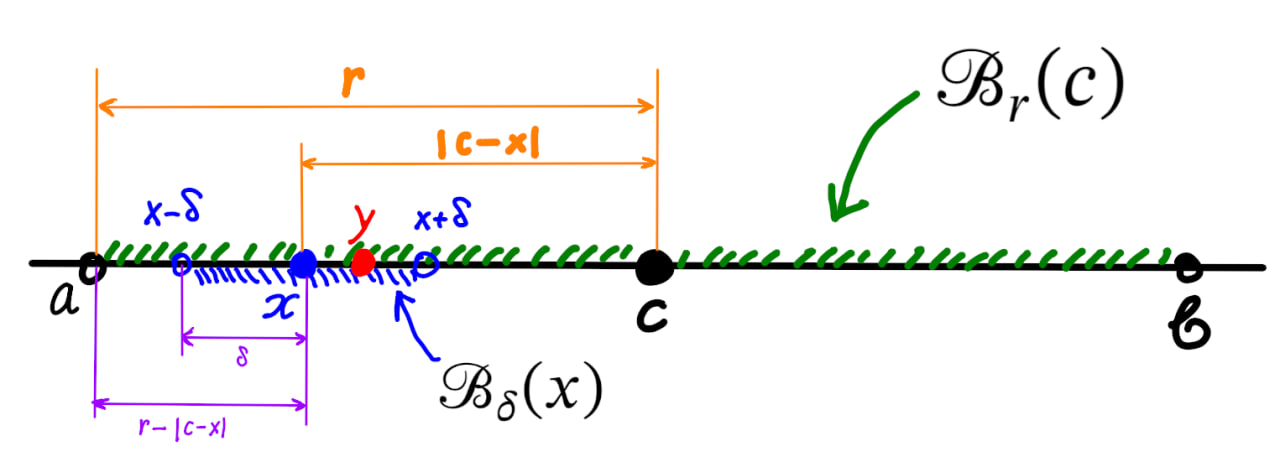
\includegraphics[scale=0.5]{images/open_is_open.jpg}
    \caption{На зелёном интервале с центром в точке $c$ мы рассматриваем произвольную синюю точку $x$ и окружаем её синей окрестностью так, чтобы она целиком была в зелёном интервале.}
    \label{fig:enter-label}
\end{figure}

Далее, используя неравенство треугольника\footnote{$|a+b|\le |a| + |b|.$}, получаем
\begin{eqnarray*}
    |c-y| &=& |c+x-x-y| \\
    &=& |(c-x) + (x-y)| \\
    &\le& |c-x| + |x-y| \\
    &<& |c-x| + \delta \\
    &<& |c-x| + r- |c-x| \\
    &=& r,
\end{eqnarray*}
\textit{т.е.} $|c-y| < r$, а значит, $y \in \mathscr{B}_r(c)$, но это и показывает, что $\mathscr{B}_\delta(x) \subseteq (a,b)$ для любой точки $x \in (a,b)$, \textit{т.е.} интервал $(a,b)$ -- открыт. Это завершает доказательство.
\end{proof}

\begin{lemma}\label{empty_is_open}
    Пустое множество открыто.
\end{lemma}

\begin{proof}
Будем рассуждать от противного. Пусть $\varnothing$ не является открытым. Тогда это значит, что найдётся хотя бы одна точка $x \in \varnothing$, что для любого $\delta >0$, $\mathscr{B}_\delta(x) \not\subseteq \varnothing$. Но в таком случае это значит, что $\varnothing$ не является пустым множеством, что даёт противоречие. Это доказывает лемму.
\end{proof}

\begin{mydanger}{\bf !}
    То рассуждение, которое было проведено, в англоязычной среде называют \textit{a vacuous proof}. 
\end{mydanger}


\begin{lemma}\label{union_and_cap_of_open}
    Объединение любого семейства открытых множеств открыто, и пересечение конечного числа открытых множеств открыто. 
\end{lemma}
\begin{proof}\
 
(1) Пусть $\mathscr{U} = \cup_{\alpha \in A}\mathscr{U}_\alpha$ и пусть $x \in \mathscr{U}$, тогда для какого-то $\alpha \in A$, $x \in \mathscr{U}_a$. Так как $\mathscr{U}_\alpha$ открыто, то найдётся такой $\varepsilon >0$, что $\mathscr{B}_\varepsilon(x) \subseteq \mathscr{U}_\alpha \subseteq \cup_{\alpha \in A}\mathscr{U}_\alpha$, что и доказывает открытость множества $\mathscr{U}.$

(2) Достаточно доказать, что пересечение двух открытых множеств $\mathscr{U}_1, \mathscr{U}_2$ открыто, а затем провести индукцию.

Если $x \in \mathscr{U}_1 \cap \mathscr{U}_2$, то найдутся такие $\varepsilon_1, \varepsilon_2 >0$, что $B_{\varepsilon_1}(x) \subseteq \mathscr{U}_1$, $B_{\varepsilon_2}(x) \subseteq \mathscr{U}_2$. Тогда, если $\varepsilon: = \min(\varepsilon_1,\varepsilon_2)$, то $B_\varepsilon(x) \subseteq \mathscr{U}_1 \cap \mathscr{U}_2$, что и доказывает открытость пересечения.
\end{proof}

\begin{mydanger}{\bf !}
    Пересечение бесконечного числа открытых множеств, вообще говоря, \textbf{не будет} открытым.
\end{mydanger}
~
\begin{example}
    Рассмотрим бесконечное семейство $\{\mathscr{U}_n\}_{n \in \mathbb{N}}$ открытых интервалов 
    \[
     \mathscr{U}_n:= \left( -\frac{1}{n}, \frac{1}{n}\right)
    \]
нетрудно видеть, что $\cap_{n=1}^\infty \mathscr{U}_n = \{0\}$, а в силу Леммы \ref{point_is_not_open}, множество $\{0\}$ не открыто.  
\end{example}


\begin{corollary}\label{R_is_open}
  Вся прямая $\mathbb{R}$ и лучи $(-\infty, a), (a, +\infty)$, $a\in \mathbb{R}$ -- открытые множества.
\end{corollary}
\begin{proof}
    Действительно, имеем
    \begin{eqnarray*}
        \mathbb{R} &=& \bigcup_{n=1}^\infty (-n,n),\\
        (-\infty, a) &=& \bigcup_{\alpha <a} (\alpha, a),\\
        (a, + \infty) &=& \bigcup_{\beta >a} (a,\beta),
    \end{eqnarray*}
    и так как каждое из множеств, участвующее в объединениях, открыто, то по лемме \ref{union_and_cap_of_open} мы получаем, что вся прямая $\mathbb{R}$ и лучи $(-\infty, a), (a, +\infty)$, $a\in \mathbb{R}$ открытые множества.
\end{proof}


\begin{definition}\label{neigh_of_point}
    \textit{Окрестностью точки} $x\in \mathbb{R}$ называется \textbf{любое} открытое множество, содержащее эту точку.
\end{definition}

Таким образом, окрестность радиуса $\varepsilon$ -- это частный случай окрестности.  

\begin{proposition}\label{open_via_open}
 Множество $\mathscr{U} \subseteq \mathbb{R}$ открыто тогда и только тогда, когда для любой точки $x$ существует такое открытое $\mathscr{V}$, что $x\in \mathscr{V} \subseteq \mathscr{U}.$
\end{proposition}

\begin{proof}~

(1) Пусть $\mathscr{U}$ -- открыто, тогда, согласно определению \ref{open_in_R}, для любой точки $x\in \mathscr{U}$ существует такая $\varepsilon$-окрестность $\mathscr{B}_\varepsilon(x)$, что $x \in \mathscr{B}_\varepsilon(x) \subseteq \mathscr{U}$, \textit{т.е.} полагая $\mathscr{V}: = \mathscr{B}_\varepsilon(x)$, что и доказывает необходимость.

(2) Пусть $\mathscr{U}$ обладает тем свойством, что для любой точки $x$ существует такое открытое $\mathscr{V}_x$, что $x\in \mathscr{V}_x \subseteq \mathscr{U}.$ Рассмотрим множество
\begin{equation}
  \widetilde{\mathscr{U}}:=\bigcup_{x\in \mathscr{U}}\mathscr{V}_x, \label{open=union_of_opens}    
\end{equation}
и покажем, что $\widetilde{\mathscr{U}} = \mathscr{U}$. Пусть $y\in \widetilde{\mathscr{U}}$, тогда существует хотя бы один $\mathscr{V}_x$, что $y \in \mathscr{V}_x$, но так как $\mathscr{V}_x \subseteq \mathscr{U}$, то $y \in \mathscr{U}$, поэтому $\widetilde{\mathscr{U}} \subseteq \mathscr{U}.$ Пусть теперь $x \in \mathscr{U}$, но тогда, согласно условию, существует такой $\mathscr{V}_x$, что $x \in \mathscr{U}_x \subseteq \mathscr{U}$, но тогда $x \in \widetilde{\mathscr{U}}$, потому что $\widetilde{\mathscr{U}} = \cup_{x \in \mathscr{U}}\mathscr{V}_x$, \textit{т.е.} $\mathscr{U} \subseteq \widetilde{\mathscr{U}}$, а значит, $\mathscr{U} = \widetilde{\mathscr{U}}.$

Так как, согласно условию, каждый $\mathscr{V}_x$ -- открытое множество, то согласно Лемме \ref{union_and_cap_of_open}, $\mathscr{U}$ -- открытое множество, что и требовалось доказать.
\end{proof}


\subsection{Внутренние и внешние точки множества}

\begin{definition}\label{interior_point}
    Точка $x$ называется \textit{внутренней точкой} множества $A \subseteq \mathbb{R}$, если существует такая окрестность $\mathscr{U}(x)$ (см. Определение \ref{neigh_of_point}) точки $x$, что $\mathscr{U}(x) \subseteq A.$ Множество всех внутренних точек множества $A$ называется \textit{внутренностью} множества $A$ и обозначается $\mathrm{Int}(A).$
\end{definition}

\begin{mydanger}{\bf !}
    Если $A \ne \varnothing$, то может быть, что $\mathrm{Int}(A) = \varnothing$. Например, если $A =\{a\}$.
\end{mydanger}


\begin{proposition}\label{int(A)_is_open}
    Для любого множества $A \subseteq \mathbb{R}$ множество $\mathrm{Int}(A)$ открыто.
\end{proposition}
\begin{proof}
Пусть $x \in \mathrm{Int}(A)$, тогда существует такая окрестность $\mathscr{U}(x)$, что $x\in \mathscr{U}(x) \subseteq A$, но согласно определению \ref{neigh_of_point}, $\mathscr{U}(x)$ -- открыто. Далее, для любой точки $y\in \mathscr{U}(x)$, мы получаем, что это же открытое множество $\mathscr{U}(x)$ есть её окрестность. Тогда для любой точки $y\in \mathscr{U}(x)$ положим $\mathscr{U}(y): = \mathscr{U}(x)$. Таким образом, все точки множества $\mathscr{U}(x)$ -- внутренние, но это значит, что $\mathscr{U}(x) \subseteq \mathrm{Int}(A)$. Теперь, воспользовавшись предложением \ref{open_via_open}, мы завершаем доказательство.
\end{proof}



\begin{proposition}\label{(U_is_open)=(U=Int(U))}
    Множество $\mathscr{U} \subseteq \mathbb{R}$ открыто тогда и только тогда, когда $\mathscr{U} = \mathrm{Int}(\mathscr{U}).$
\end{proposition}

\begin{proof}
    Действительно, согласно предложению \ref{int(A)_is_open}, множество $\mathrm{Int}(\mathscr{U})$ -- открыто. Далее, если $\mathscr{U}$ -- открыто, то в силу определения \ref{open_in_R}, каждая его точка -- внутренняя, что и означает $\mathscr{U} = \mathrm{Int}(\mathscr{U})$. Если же $\mathscr{U} = \mathrm{Int}(\mathscr{U})$, то каждая точка множества $\mathscr{U}$ является внутренней, но тогда, согласно определению \ref{interior_point}, это означает, что существует $\varepsilon$-окрестность этой точки которая целиком будет лежать в $\mathscr{U}$, \textit{т.е.} согласно определению \ref{open_in_R} означает открытость $\mathscr{U}$.
\end{proof}

\begin{example}\label{(a,b)c(open}
    Согласно определению, имеем
    \begin{eqnarray*}
        \mathrm{Int}([a,b]) &=& (a,b),\\
        \mathrm{Int}([a,b)) &=& (a,b),\\
        \mathrm{Int}((a,b]) &=& (a,b),\\
        \mathrm{Int}((a,b)) &=& (a,b),
    \end{eqnarray*}
потому что ни $a$, ни $b$ не могут быть внутренними точками этих множеств; любая их $\varepsilon$-окрестность не может содержаться в этих множествах.

Таким образом, согласно предложению $\ref{(U_is_open)=(U=Int(U))}$, множества
\[
 [a,b], \qquad [a,b), \qquad (a,b]
\]
не являются открытыми, а множество $(a,b)$ -- открыто.
\end{example}

\begin{example}\label{(a,8)c(open)}
    Рассмотрим теперь множества $(a, +\infty)$, $[a,\infty)$, $(-\infty, b)$,  $(-\infty,b]$. Так как для точек $a,b$ любая их $\varepsilon$-окрестность не может содержаться в этих множествах, то получаем
    \begin{eqnarray*}
        \mathrm{Int}((a, +\infty)) &=& (a, +\infty), \\
        \mathrm{Int}([a, +\infty)) &=& (a, +\infty), \\
        \mathrm{Int}((-\infty, b)) &=& (-\infty, b), \\
        \mathrm{Int}((-\infty, b]) &=& (-\infty, b),
    \end{eqnarray*}
тогда, согласно предложению \ref{(U_is_open)=(U=Int(U))}, множества
\[
 [a, +\infty), \qquad (-\infty, b]
\]
не являются открытыми, а множества  $(a, +\infty)$, $(-\infty, b)$ -- открыты.
\end{example}


\begin{definition}
    Внутренняя точка множества $\mathbb{R}\setminus A$ называется \textit{внешней точкой} множества $A$, а внутренность множества $\mathbb{R}\setminus A$ называется \textit{множеством внешних точек} множества $A$.
\end{definition}



\subsection{Замкнутые множества}

\begin{definition}\label{def_of_closed}
    \textit{Замкнутое множество} в $\mathbb{R}$ есть дополнение открытого множества. 
\end{definition}

\begin{lemma}
Пустое множество $\varnothing$ и вся прямая $\mathbb{R}$ -- замкнутые множества.
\end{lemma}

\begin{proof}
    Действительно, согласно лемме \ref{empty_is_open}, множество $\varnothing$ -- открыто в $\mathbb{R}$, а так как $\mathbb{R} = \mathbb{R}\setminus \varnothing$, то значит, $\mathbb{R}$ -- замкнуто. Далее, согласно следствию \ref{R_is_open}, множество $\mathbb{R}$ -- открыто, а так как $\varnothing = \mathbb{R} \setminus \mathbb{R}$, то значит, множество $\varnothing$ -- замкнуто.
\end{proof}

\begin{mydanger}{\bf!}
Таким образом, множества $\mathbb{R}$, $\varnothing$ одновременно и открыты, и замкнуты; и вообще, не следует считать, что замкнутость -- это отрицание открытости.
\end{mydanger}

\begin{example}\label{[a,b]is_closed}
Рассмотрим множества $[a,b]$, $[a,+\infty)$ и $(-\infty, b]$.

Имеем
\begin{eqnarray*}
    [a,b] &=& \mathbb{R}\setminus ((-\infty, a) \cup (b, +\infty)),\\
    {[a,+\infty)} &=& \mathbb{R} \setminus (-\infty, a),\\
    {(-\infty, a]} &=& \mathbb{R} \setminus (a, +\infty),
\end{eqnarray*}
а так как согласно примерам \ref{(a,b)c(open}, \ref{(a,8)c(open)}, множества $(-\infty, a),$ $(b, +\infty)$ открыты, то множества $[a,b]$, $[a,+\infty)$ и $(-\infty, a]$ -- замкнуты.
\end{example}

\begin{lemma}
    Пересечение любого семейства замкнутых множеств замкнуто, а объединение конечного числа замкнутых замкнуто.
\end{lemma}

\begin{proof}
Пусть $\{F_\alpha\}_{\alpha \in A}$ -- какое-то семейство замкнутых множеств, тогда, согласно определению \ref{def_of_closed}, имеется семейство открытых множеств $\{\mathscr{U}_\alpha\}_{\alpha \in A}$, что $F_\alpha = \mathbb{R}\setminus \mathscr{U}_\alpha$ для любого $\alpha \in A.$

Согласно (\ref{dM1}), (\ref{dM1}) получаем
\begin{eqnarray*}
 \bigcup_{i=1}^n F_i &=& \bigcup_{i=1}^n \mathbb{R} \setminus \mathscr{U}_i =  \mathbb{R} \setminus \bigcap_{i=1}^n\mathscr{U}_i, \\
 \bigcap_{\alpha \in A} F_\alpha &=& \bigcap_{\alpha \in A} \mathbb{R} \setminus \mathscr{U}_\alpha = \mathbb{R} \setminus \bigcup_{\alpha \in A} \mathscr{U}_\alpha,   
\end{eqnarray*}
но согласно \ref{union_and_cap_of_open}, множества $\cap_{i=1}^n\mathscr{U}_i$, $\cup_{\alpha \in A} \mathscr{U}_\alpha$ -- открыты, что и завершает доказательство.
\end{proof}

\begin{mydanger}{\bf !}
    Объединение бесконечного числа замкнутых, вообще говоря, не замкнуто. Более того, такое объединение может быть открытым множеством. Например, $\cup_{n=1}^\infty \left[\frac{1}{n},1-\frac{1}{n} \right] = (0,1).$
\end{mydanger}

\begin{lemma}
    Множество $\{a\}$ является замкнутым множеством в $\mathbb{R}$.
\end{lemma}

\begin{proof}
    Действительно, имеем
    \[
    \{a\} = \mathbb{R}\setminus \left( (-\infty, a) \cup (a, +\infty) \right),
    \]
согласно следствию \ref{R_is_open}, множества $(-\infty, a),$ $(a, +\infty)$ -- открыты, а по предложению \ref{union_and_cap_of_open}, множество $(-\infty, a) \cup (a, +\infty)$ -- открыто, что и доказывает лемму.
\end{proof}

\begin{mydanger}{\bf !}
Таким образом, любое множество $A$ в $\mathbb{R}$ можно представить как объедение замкнутых множеств, так как $A = \cup_{a \in A}\{a\}.$
\end{mydanger}

\begin{definition}\label{limit_point}
  \textit{Точка прикосновения} множества $A$ -- это такая точка $x \in \mathbb{R}$, каждая окрестность которой имеет с $A$ непустое пересечение. Множество всех точек прикосновения называется \textit{замыканием} множества $A$ и обозначается символом $\overline{A}.$
\end{definition}

\begin{mydanger}{\bf !}
    Таким образом, любая точка $a\in A$ есть точка прикосновения, а обратное, конечно же, неверно.
\end{mydanger}

\begin{remark}
Сказать, что \textit{$x$ не является} точкой прикосновения множества $A$, значит сказать, что $x$ является внутренней точкой множества $\mathbb{R}\setminus A.$ 
\end{remark}

\begin{proposition}\label{closure(A)=R-(R-A)}
Для любого множества $A \subseteq \mathbb{R}$, $\overline{A} = \mathbb{R}\setminus \mathrm{Int}(\mathbb{R}\setminus A).$    
\end{proposition}

\begin{proof}
Мы воспользуемся следующим фактом: $X = Y$ тогда и только тогда, когда $E\setminus X = E \setminus Y$, где $X,Y \subseteq E$.

Поэтому нам достаточно показать, что $\mathbb{R} \setminus \overline{A} = \mathrm{Int}( \mathbb{R}\setminus A).$

Если $x \in \mathbb{R} \setminus \overline{A}$, то $x \notin \overline{A}$, а это значит, что существует такая окрестность $\mathscr{U}(x)$, что $\mathscr{U}(x) \cap A = \varnothing$, \textit{т.е.} $\mathscr{U}(x) \subseteq \mathbb{R}\setminus A$, а тогда это значит, что $x \in \mathrm{Int}(\mathbb{R} \setminus A)$, поэтому $\mathbb{R} \setminus \overline{ A} \subseteq \mathrm{Int}(\mathbb{R} \setminus A).$

Если $x \in \mathrm{Int}(\mathbb{R} \setminus A)$, то найдётся такая её окрестность $\mathscr{U}(x)$, что $\mathscr{U}(x) \subseteq \mathbb{R}\setminus A$, \textit{т.е. } $\mathscr{U}(x) \cap A = \varnothing $, а это значит, что $x$ не может быть точкой прикосновения, \textit{т.е.} $x \in \mathbb{R}\setminus \overline{A}$, поэтому $\mathbb{R} \setminus \overline{ A} \supseteq \mathrm{Int}(\mathbb{R} \setminus A)$, что и доказывает утверждение.
\end{proof}

\begin{corollary}
 Для любого $A\subseteq \mathbb{R}$, множество $\overline{A}$ -- замкнуто. \end{corollary}
\begin{proof}
    Согласно предложению \ref{closure(A)=R-(R-A)}, $\overline{A} = \mathbb{R}\setminus \mathrm{Int}(\mathbb{R}\setminus A)$, а согласно предложению \ref{int(A)_is_open}, множество $ \mathrm{Int}(\mathbb{R}\setminus A)$ открыто, поэтому $\overline{A}$ -- замкнуто.
\end{proof}
    
\begin{example}~
 Рассмотрим множества $(a,b), (a,b], [a,b), [a,b]$, точки $a,b$ являются точками прикосновения для обоих этих множеств, так как любая $\varepsilon$-окрестность (а значит, и любая вообще) этих точек имеет непустое пересечение, например,
 \[
  (a-\varepsilon, a+\varepsilon)\cap (a,b] = \begin{cases}
      (a,a+\varepsilon], & a+\varepsilon \le b \\
      (a,b], & a+\varepsilon > b, 
  \end{cases}
 \]
 поэтому $\overline{(a,b)} = \overline{(a,b]} = \overline{[a,b)} = \overline{[a,b]} = [a,b].$
\end{example}

\begin{definition}
    Операция $A \mapsto \overline{A}$ называется замыканием множества $A\subseteq \mathbb{R}.$
\end{definition}


\begin{lemma}\label{closure}
    Множество $F$ замкнуто, если и только если все его точки -- это точки прикосновения, \textit{т.е.} $F = \overline{F}.$ 
\end{lemma}
\begin{proof}~
 (1) Пусть $F$ -- замкнуто, тогда найдётся какое-то открытое $\mathscr{U} \subseteq \mathbb{R}$ такое, что $F  = \mathbb{R} \setminus \mathscr{U}$. Пусть $x \notin F$, тогда $x \in \mathscr{U}$, и тогда найдётся окрестность $\mathscr{U}(x)$ такая, что $\mathscr{U}(x) \subseteq \mathscr{U}$, потому что $\mathscr{U}$ -- открыто, \textit{т.е.} $\mathscr{U}(x) \cap F = \varnothing.$ Таким образом, получили, что если $F$ -- замкнуто, то никакая точка $x \notin F$ не может быть точкой прикосновения для $F$, \textit{т.е.} $F = \overline{F}.$ 

(2) Пусть $F = \overline{F}$, тогда если $x \notin F$, то $x$ не может быть точкой прикосновения для $F$, а это значит, что можно найти окрестность $\mathscr{U}(x)$ такую, что $\mathscr{U}(x) \cap F = \varnothing$, иначе $x$ было бы точкой прикосновения. Итак, для любого $x \notin F$, мы имеем окрестность $\mathscr{U}(x)$ такую, что $\mathscr{U}(x) \cap F = \varnothing$. Рассмотрим теперь объединения всех таких окрестностей,
\[
 \mathscr{U}:= \bigcup_{x \in \mathbb{R}\setminus F} \mathscr{U}(x),
\]
так как каждое $\mathscr{U}(x)$ открыто, то согласно лемме \ref{union_and_cap_of_open}, $\mathscr{U}$ -- открыто. 

Покажем, что $F = \mathbb{R} \setminus \mathscr{U}$, согласно (\ref{dM1})
\[
 \mathbb{R} \setminus \mathscr{U} = \mathbb{R} \setminus \bigcup_{x \in \mathbb{R}\setminus F} \mathscr{U}(x) = \bigcap_{x \in \mathbb{R} \setminus F} \mathbb{R} \setminus \mathscr{U}(x).
\]

Пусть $y \in F$, тогда $y \notin \mathscr{U}$, а тогда $y \in \mathbb{R}\setminus \mathscr{U}$, поэтому $F \subseteq \mathbb{R} \setminus \mathscr{U}$. Если $y \in \mathbb{R}\setminus \mathscr{U}$, то $y \in \cap_{x \in \mathbb{R} \setminus F} \mathbb{R} \setminus \mathscr{U}(x)$, \textit{т.е.} для любого $x \notin F$, $y \in \mathbb{R}\setminus \mathscr{U}(x)$, \textit{т.е.} $y \notin \mathscr{U}(x)$, но это значит, что $y \ne x$ для любого $x \notin F$, а тогда $y \in F$. Таким образом, $F \supseteq \mathbb{R} \setminus \mathscr{U}$, поэтому $F = \mathbb{R}\setminus \mathscr{U}.$ Это завершает доказательство леммы.
\end{proof}

\begin{mydanger}{\bf !}
    Множества $(a,b]$, $[a,b)$ и не открыты, и не замкнуты в $\mathbb{R}$, а множества $\varnothing,$ $\mathbb{R}$ и открыты, и замкнуты одновременно.
\end{mydanger}



\section{Лекция \#11. Компактность на прямой}

Прежде всего, мы разберём топологию подмножеств на вещественной прямой. 

\subsection{Открытость и замкнутость в подмножествах}

\begin{definition}\label{e-neigh_in_A}
    Пусть $A \subseteq \mathbb{R}$ -- непустое подмножество в $\mathbb{R}$, \textit{$\varepsilon$-окрестностью точки $a \in A$ в множестве $A$} называется множество вида $(a-\varepsilon, a+\varepsilon) \cap A$. Чтобы подчеркнуть, что рассматривается $\varepsilon$-окрестность в $A$, мы будем писать $\mathscr{B}_\varepsilon(a)|_A$. Таким образом, согласно определению,
    \[
     \mathscr{B}_\varepsilon(a)|_A: = \mathscr{B}_\varepsilon(a) \cap A.
     \]
 
Далее, множество $\mathscr{U} \subseteq A$ называется \textit{открытым в $A$}, если для любой точки $x \in \mathscr{U}$ найдётся такая $\varepsilon$-окрестность $\mathscr{B}_\varepsilon(x)|_A$, что $\mathscr{B}_\varepsilon(x)|_A \subseteq \mathscr{U}$.
 \end{definition}

\begin{mydanger}{\bf{!}}
    Обратим внимание, что если $A = \mathbb{R}_{\ge 0} \subseteq \mathbb{R}$, то, например, $[0,1)$ -- открытый шар в $A = \mathbb{R}_{\ge 0}$, так как $[0,1) = (-1,1) \cap \mathbb{R}_{\ge 0}$. Hо! В $\mathbb{R}$, $[0,1)$ и не открыт, и не замкнут!
\end{mydanger}

\begin{theorem}\label{open_in_K}
    Для того, чтобы множество $\mathscr{U} \subseteq A$ было открыто в $A$, необходимо и достаточно, чтобы существовало такое открытое в $\mathbb{R}$ множество $\widetilde{\mathscr{U}} \subseteq \mathbb{R}$, что $\mathscr{U} = \widetilde{\mathscr{U}}\cap A.$
\end{theorem}

\begin{proof}~

(1) Пусть $\mathscr{U}$ открыто в $A$, это значит, что для любой точки $x \in \mathscr{U}$ можно найти $\varepsilon$-окрестность $\mathscr{B}_\varepsilon(x)|_A$ такую, что $\mathscr{B}_\varepsilon(x)|_A \subseteq \mathscr{U}$, \textit{т.е.,} $\mathscr{B}_\varepsilon(x) \cap A \subseteq \mathscr{U}$.

Так как $\mathscr{U} = \cup_{x \in \mathscr{U}} \mathscr{B}_\varepsilon(x) \cap A$, то получаем следующее:

\[
 \mathscr{U} = \bigcup_{x \in \mathscr{U}} \mathscr{B}_\varepsilon(x) \cap A = A \cap \left( \bigcup_{x \in \mathscr{U}} \mathscr{B}_\varepsilon(x) \right) =  A \cap \widetilde{\mathscr{U}},
\]
где $\widetilde{\mathscr{U}}: = \cup_{x\in \mathscr{U}} \mathscr{B}_\varepsilon(x) \subseteq \mathbb{R}$. Согласно леммам \ref{interval_is_open}, \ref{union_and_cap_of_open}, множество $\widetilde{\mathscr{U}}$ -- открыто в $\mathbb{R}$, что и доказывает необходимость.


(2) Пусть $\widetilde{\mathscr{U}}$ -- открытое множество в $\mathbb{R}$, и пусть $x \in \widetilde{\mathscr{U}} \cap A$. Так как $\widetilde{\mathscr{U}}$ -- открыто в $\mathbb{R}$, то найдётся $\varepsilon$-окрестность $\mathscr{B}_\varepsilon(x) \subseteq \mathbb{R}$ такая, что $\mathscr{B}_\varepsilon(x) \subseteq \widetilde{\mathscr{U}}$. Тогда $A \cap \mathscr{B}_\varepsilon(x) \subseteq A \cup \widetilde{\mathscr{U}}$. Но согласно определению \ref{e-neigh_in_A}, $\mathscr{B}_\varepsilon(x)\cap A = : \mathscr{B}_\varepsilon(x)|_A$. Тогда включение $A \cap \mathscr{B}_\varepsilon(x) \subseteq A \cup \widetilde{\mathscr{U}}$ и означает, что $\widetilde{\mathscr{U}} \cap A$ открыто в $A$, ибо $x$ -- произвольная точка в $\widetilde{\mathscr{U}} \cap A.$
\end{proof}

\begin{definition}\label{closed_in_A}
    Пусть $A \subseteq \mathbb{R}$ -- непустое множество, множество $F \subseteq A$ называется \textit{замкнутым в $A$}, если существует такое открытое множество $\mathscr{U}$ в $A$, что $F = A \setminus \mathscr{U}$. 
\end{definition}

\begin{remark}
    Иногда также говорят об относительной открытости или относительной замкнутости какого-то множества относительно выделенного подмножества.
\end{remark}

\begin{proposition}\label{closed_in_A_if}
    Множество $F$ замкнуто в $A$ тогда и только тогда, когда существует такое замкнутое $\widetilde{F}$ в $\mathbb{R}$ множество, что $F  = A \cap \widetilde{F}.$
\end{proposition}

\begin{proof}
    Нам понадобится равенство 
\begin{equation}\label{good_for_us}
     B \cap (\mathbb{R} \setminus C) = B \setminus (B \cap C),
\end{equation}
которое верно для любых подмножеств $B,C \subseteq \mathbb{R}$.
Действительно, если $x \in B \cap (\mathbb{R} \setminus C)$, то $x \in B$ и $x \in \mathbb{R} \setminus C$, \textit{т.е.} $x \notin C$, а это значит, что $x \in B \setminus (B \cap C)$. Наоборот, если $x \in B \setminus (B \cap C)$, то $x \in B$, но $x \notin B \cap C$, \textit{т.е.} $x \notin C$, а это значи, что $x \in \mathbb{R} \setminus C$.

(1) Пусть $F$ -- замкнуто в $A$, тогда (см. Определение \ref{closed_in_A}), $A\setminus F$ -- открыто в $A$, а тогда, согласно теореме \ref{open_in_K}, существует такое открытое в $\mathbb{R}$ множество $\mathscr{U}$, что $A \setminus F = A \cap \mathscr{U}$. Пусть $\widetilde{F}: = \mathbb{R} \setminus\mathscr{U}$, тогда, согласно определению \ref{def_of_closed}, $\widetilde{F}$ -- замкнуто в $\mathbb{R}$, а согласно (\ref{good_for_us}), имеем
\[
 A \cap \widetilde{F} = A \cap (\mathbb{R}\setminus \mathscr{U}) = A \setminus (A \cap \mathscr{U}) = A\setminus(A \setminus F) = F, 
\]
что и требовалось доказать.

(2) Пусть теперь $\widetilde{F}$ -- замкнутое множество в $\mathbb{R}$, покажем, что $\widetilde{F} \cap A$ -- замкнуто в $A.$ Согласно определению \ref{def_of_closed}, найдётся такое открытое в $\mathbb{R}$ множество $\mathscr{U}$, что $\widetilde{F} = \mathbb{R}\setminus \mathscr{U}$, тогда, воспользовавшись равенством (\ref{good_for_us}), имеем
\[
  A \cap \widetilde{F} = A \cap (\mathbb{R}\setminus \mathscr{U}) = A \setminus (A \cap \mathscr{U}),
\]
но согласно теореме \ref{open_in_K}, множество $A \cap \mathscr{U}$ -- открыто в $A$, а тогда, согласно определению \ref{closed_in_A}, множество $A \setminus (A \cap \mathscr{U})$ -- замкнуто в $A$. Тем самым предложение полностью доказано.
\end{proof}


\subsection{Понятие компактности}

\begin{definition}~

Пусть $X$ -- произвольное непустое множество. Множество $(\mathscr{U}_\lambda)_{\lambda \in \Lambda}$ подмножеств множества $X$ называется его \textit{покрытием}, если $X = \bigcup_{\lambda \in \Lambda} \mathscr{U}_\lambda$.    

Если $X \subseteq Y$, то множество $(\mathscr{U}_\lambda)_{\lambda \in \Lambda}$ подмножеств множества $Y$ называется \textit{покрытием} множества $X\subseteq Y$, если $X \subseteq \bigcup_{\lambda \in \Lambda} \mathscr{U}_\lambda$.

Если $(\mathscr{U}_\lambda)_{\lambda \in \Lambda}$ -- покрытие для $X$, то подпокрытием называют какие-то части этого покрытия, \textit{т.е.} если существует такое $\Lambda' \subseteq \Lambda$, что $X = \bigcup_{\lambda \in \Lambda '}\mathscr{U}_{\lambda}$.
\end{definition}


\begin{example}
    Пусть $X = \mathbb{R}$, и $\mathscr{U}_\alpha: = (-\alpha, \alpha)$, где $\alpha$ -- любое ненулевое положительное вещественное число, тогда ясно что $\mathbb{R}  = \cup_{\alpha \in \mathbb{R}} (-\alpha, \alpha)$. Таким образом, мы получили покрытие $\{(-\alpha ,\alpha)\}_{\alpha \in \mathbb{R}_+}$. Если теперь мы ограничимся рассмотрением только рациональных чисел, \textit{т.е.} рассмотрением интервалов $(-r, r)$, где $r \in \mathbb{Q}_+$, то мы получаем подпокрытие $\{(-r, r)\}_{r\in \mathbb{Q}_+}$ для $\mathbb{R}$, ведь $\mathbb{R} = \cup_{r\in \mathbb{Q}_+}(-r,r)$. В этом случае $\Lambda = \mathbb{R}_+$, $\Lambda'= \mathbb{Q}_+$. Можно рассмотреть только целые положительные числа, и тогда получаем ещё одно подпокрытие $\{(-n,n)\}_{n \in \mathbb{N}}$ для $\mathbb{R}$.
\end{example}


\begin{example}
    Пусть $X = [0,1)$, $Y = \mathbb{R}$, ясно, что $X \subseteq Y$. Тогда, например, множества
   \[
   \{(-1,2), (0,5)\},\qquad  \{(-n,n)\}_{n \in \mathbb{N}}, \qquad \left\{\left[0,1-\frac{2}{n}\right)\right\}_{n \in \mathbb{N}},  
   \] 
являются покрытиями для $X$ множествами из $Y$, так как
\[
 [0,1) \subseteq (-1,2) \cup (0,5), \qquad [0,1) \subseteq \bigcup_{n \in \mathbb{N}} (-n,n), \qquad [0,1) \subseteq \bigcup_{n \in \mathbb{N}}\left[0,1-\frac{2}{n}\right),
\]
а так как 
\[
 [0,1) = \bigcup_{n \in \mathbb{N}}\left[0,1-\frac{2}{n}\right),
\]
то последнее множество -- это есть просто покрытие для $X$, так как все $\left[0,1-\frac{2}{n}\right)$ находятся в $X$.
\end{example}


\begin{definition}
Непустое множество $K \subseteq \mathbb{R}$ называется \textit{компактным}, если в любом его открытом покрытии всегда можно найти подпокрытие, состоящее из конечного числа множеств.
\end{definition}

\begin{comments}
   Другими словами, это означает следующее: если множество $K$ компактно, то \textbf{какое бы бесконечное} покрытие мы не придумали для него, \textbf{ВСЕГДА} из этого покрытия можно выделить конечный набор множеств, которые покроют весь $K$.
\end{comments}

\begin{mydanger}{\bf !}
На самом деле свойство быть компактным является ``внутренним'' свойством этого множества, \textit{т.е.} неважно покрываем мы его открытыми множествами во всей прямой или же только открытыми в нём.
\end{mydanger}

\begin{theorem}
    Пусть $K\subseteq \mathbb{R}$ -- непустое множество, тогда следующие условия равносильны;
    \begin{enumerate}
        \item[(1)] для любого открытого покрытия для $K$ можно всегда найти конечное подпокрытие для $K$,
        \item[(2)] для любого открытого в $K$ покрытия для $K$ можно всегда найти конечное подпокрытие для $K$.
    \end{enumerate}
\end{theorem}

\begin{proof}~

$(1) \Longrightarrow (2).$ Пусть $K$ -- компактно, это значит, что для любого покрытия $\{\widetilde{\mathscr{U}}_\alpha\}_{\alpha \in A}$ множества $K$ открытыми множествами в $\mathbb{R}$ можно всегда найти конечное подпокрытие, скажем, $K \subseteq \cup_{i=1}^n \widetilde{\mathscr{U}}_i$, но тогда 
\[
 K = K \cap \bigcup_{i=1}^n \widetilde{\mathscr{U}}_i= \bigcup_{i=1}^n \mathscr{U}_i
\]
но, согласно определению \ref{e-neigh_in_A}, каждое $\mathscr{U}_\alpha : = \widetilde{\mathscr{U}}_\alpha \cap K$ -- открыто в $K$, \textit{т.е.} из (1) получаем (2).

$(1) \Longleftarrow (2).$ Пусть $\{ \mathscr{U}_\alpha \}_{\alpha \in A}$ -- покрытие $K$, \textit{т.е.} $K = \cup_{\alpha \in A} \mathscr{U}_\alpha$, где все $\mathscr{U}_\alpha \subseteq K$ открыты в $K$, но тогда (см. Теорему \ref{open_in_K}) для каждого $\alpha \in A$ существует открытое множество $\widetilde{\mathscr{U}}_\alpha$ в $\mathbb{R}$ такое, что $\mathscr{U}_\alpha= \widetilde{\mathscr{U}}_\alpha \cap K$. Тогда $K \subseteq \cup_{\alpha \in A} \widetilde{\mathscr{U}}_\alpha.$ Так как по условию (2), можно найти конечное число множеств, скажем, $\mathscr{U}_1, \ldots, \mathscr{U}_n$, таких, что $K = \cup_{i=1}^n\mathscr{U}_i$, то тогда $K \subseteq \cup_{i=1}^n \widetilde{\mathscr{U}}_i$, что и показывает (1).
\end{proof}


\begin{theorem}\label{[a,b]is_compact}
    Любой отрезок $[a,b] \subsetneq \mathbb{R}$ конечной длины $a<b$, является компактным множеством.
\end{theorem}

\begin{proof}
Доказывать будем от противного. Допустим, что существует такое покрытие $\{\mathscr{U}_\alpha\}_{\alpha \in A}$ открытыми множествами из $\mathbb{R}$ для отрезка $I = [a,b]$, что из него нельзя выбрать конечное подпокрытие. 

Итак, пусть $I \subseteq \bigcup_{\alpha \in A} \mathscr{U}_\alpha$ и из этого покрытия нельзя выбрать конечное подпокрытие, которое бы покрыло $I$. Разобьём $I$ пополам \textit{т.е} представим его так:
    \[
     [a, b] = \left[ a, \frac{a+b}{2} \right] \cup \left[\frac{a+b}{2}, b \right].
    \]


По условию $I$ нельзя покрыть конечным числом множеств из $\{ \mathscr{U}_\alpha\}_{\alpha \in A}$, тогда хотя бы один из полученных отрезков, обозначим его через $I_1$ тоже нельзя покрыть конечным числом множеств из покрытия $\{ \mathscr{U}_\alpha\}_{\alpha \in A}$. Иначе бы оба полученных отрезка покрывались бы конечным числом множества из покрытия, а тогда и $I$ покрывался бы конечным числом множеств из этого покрытия, что и показывала бы компактность $I$. 

Разобьём теперь отрезок $I_1$ аналогичным образом на два равных отрезка. Так как $I_1$ нельзя покрыть конечным числом множеств из покрытия $\{ \mathscr{U}_\alpha\}_{\alpha \in A}$, то найдётся хотя бы один, скажем, $I_2$, из только что полученных, который тоже нельзя покрыть конечным числом множеств. Будем повторять эту процедуру каждый раз, пусть $I_k = [a_k,b_k]$, $k\ge 1$. В результате мы получаем бесконечную цепь вложенных друг в друга отрезков 
\[
 I \supsetneq I_1 \supsetneq I_2 \supsetneq \ldots,
\]
каждый из которых нельзя покрыть конечным числом элементов множества $\{\mathscr{U}_\alpha\}_{\alpha \in A}$. Более того, их длины строго уменьшаются (каждый из отрезков по длине в два раза меньше, чем предыдущий). Тогда по Лемме о вложенных отрезках (Лемма \ref{cap_of_intervals}), существует такая точка $c \in I$, что $c \in \bigcap_{k \ge 1} I_k $,
которая есть предел для последовательности их концов;
\[
 \lim_{k\to \infty }a_k  = c = \lim_{n \to \infty}b_n.
\]

Тогда для любого $\varepsilon >0$ найдётся такой номер $N$, что при $k \ge N$ все $a_k, b_k \in (c - \varepsilon, c + \varepsilon)$, а по построению это значит, что и все $I_k \subseteq (c-\varepsilon, c+\varepsilon)$, $k \ge N.$

С другой стороны, так как имеется покрытие $\{\mathscr{U}_\alpha\}_{\alpha \in A}$ этого отрезка $I$, то найдётся хотя бы одно открытое множество $\mathscr{U}_\alpha$ такое, что $c \in \mathscr{U}_\alpha.$, а так как оно открытое, то для точки $c$ можно найти $\varepsilon$-окрестность $(c-\varepsilon, c+ \varepsilon) \subseteq \mathscr{U}_\alpha.$ 

Таким образом, мы получаем, что для всех $k \ge N$ есть включения
\[
 I_k \subseteq (c-\varepsilon, c+ \varepsilon) \subseteq \mathscr{U}_\alpha,
\]
но это значит, что все отрезки $I_k$ покрываются всего одним открытым множеством $\mathscr{U}_\alpha$, что противоречит построению отрезков $I_k$, \textit{т.е.} такое построение невозможно, что и означает компактность отрезка $I.$
\end{proof}

Теперь у нас всё готово, чтобы описать компактные множества в $\mathbb{R}$.

\begin{theorem}[\textbf{Свойства компакта}]\label{properties_of_compact_in_R}
Любое компактное множество $K$ в $\mathbb{R}$ обладает следующими свойствами;
  \begin{enumerate}
      \item $K$ -- ограниченное множество.
      \item $K$ -- замкнутое множество
      \item Любое замкнутое в $K$ подмножество множества $K$ компактно.
  \end{enumerate} 
\end{theorem}

\begin{proof}~

(1)  Рассмотрим произвольную точку $x\in K$ и рассмотрим такое открытое покрытие $\{(x-n,x+n)\}_{n=1}^\infty$ для $K$. Так как $K$ -- компактно, то из этого покрытия можно выбрать конечное подпокрытие, скажем, $\{ (x-r,x+r) \}_{r=t}^N$, такое, что $K \subseteq \cup_{t=1}^N  (x-t, x+t)$. Так как $(x-p,x+p) \subseteq (x-q,x+q)$ при $p<q$, то $\cup_{t=1}^N  (x-t, x+t) = (x_N, x+N)$, \textit{т.е.} $K \subseteq (x-N, x+N)$, что и означает ограниченность $K.$

(2) Пусть $y \in \overline{K}$, но $y \notin K$. Для каждого $x\in K$ рассмотрим числа $\delta_x, \varepsilon_x >0$, чтобы $\delta_x + \varepsilon_x < |x-y|$, тогда $(x-\delta_x, x+\delta_x) \cap (y-\varepsilon_x, y+\varepsilon_x) = \varnothing.$ Ясно, что $K \subseteq \cup_{x \in K} (x-\delta_x, x+\delta_x)$ и так как $K$ -- компактно, то можно найти конечное множество точек $\{x_1,\ldots, x_n\}$ такое, что $K \subseteq \cup_{i=1}^n (x_i-\delta_i, x_i+\delta_i)$, где $\delta_i := \delta_{x_i}$, $1\le i \le n.$ Для всех таких $x_i$ мы выбираем $\varepsilon_i>0$ так, чтобы $(y-\varepsilon_i, y+\varepsilon_i) \cap (x_i-\delta_i, x_i+\delta_i = \varnothing$. Но тогда, полагая $\varepsilon: = \min \{\varepsilon_1, \ldots, \varepsilon_n\}$, получаем, что
\[
  (y-\varepsilon, y+\varepsilon) \cap K \subseteq (y-\varepsilon, y+\varepsilon) \cap \bigcup_{i=1}^n (x_i - \delta_i, x_i+ \delta_i) = \varnothing,
\]
\textit{т.е.} мы нашли $\varepsilon$-окрестность $(y-\varepsilon, y+\varepsilon)$ точки $y$, которая не пересекается с $K$. Но это означает (см. Определение \ref{limit_point}, Лемма \ref{closure}), что $y \notin \overline{K}$.  Поэтому если $y\in \overline{K}$, то $y \in K$, \ie $\overline{K} = K.$



(3) Пусть $F \subseteq K$ -- замкнутое подмножество в $K$, и пусть $\{\mathscr{U}_\alpha\}_{\alpha \in A}$ -- покрытие $F$ открытыми множествами в $K$, \textit{т.е.} $F \subseteq \cup_{\alpha \in A} \mathscr{U}_\alpha$.

Тогда имеем
\[
  K = F \cup (K \setminus F) \subseteq \bigcup_{\alpha \in A} \mathscr{U}_\alpha \cup (K \setminus F),
\]
но ясно, что $K = \bigcup_{\alpha \in A} \mathscr{U}_\alpha \cup (K \setminus F)$, потому что если есть $x \in \bigcup_{\alpha \in A} \mathscr{U}_\alpha \cup (K \setminus F)$, но $x \notin 
K$, то это значит, что найдётся хотя бы один $\mathscr{U}_\alpha$, что $x \in \mathscr{U}_\alpha$, но все $\mathscr{U}_\alpha \subseteq K$ -- открытые подмножества, поэтому $K = \bigcup_{\alpha \in A} \mathscr{U}_\alpha \cup (K \setminus F).$

Таким образом, мы получили покрытие для $K$, но так как $K$ -- компактно, то можно найти такие, скажем, $\mathscr{U}_1, \ldots, \mathscr{U}_n$, что 
\[
 K = \mathscr{U}_1 \cup \cdots \cup \mathscr{U}_n \cup (K \setminus F),
\]
но тогда 
\[
 F \subseteq \mathscr{U}_1 \cup \cdots \cup \mathscr{U}_n,
\]
что означает компактность $F.$
\end{proof}

\begin{theorem}[{\bf Критерий компактности в $\mathbb{R}$}]\label{criterai_of_compacness_in_R}
Множество $K \subseteq \mathbb{R}$ компактно тогда и только тогда, когда оно замкнуто и ограничено.    
\end{theorem}
\begin{proof}~

(1) Согласно Теореме \ref{properties_of_compact_in_R} (1), мы получаем необходимость.

(2) Если $K \subseteq \mathbb{R}$ ограничено и замкнуто, то это значит, что оно содержится в некотором отрезке $I$, который в силу Теоремы \ref{[a,b]is_compact} является компактным в $\mathbb{R}$. Далее, отрезок $I$ -- замкнут (см. Пример \ref{[a,b]is_closed}), а так как $K = I \cap K$, то согласно предложению \ref{closed_in_A_if}, $K$ -- замкнут в $I$. Наконец, из теоремы \ref{properties_of_compact_in_R} (3) вытекает утверждение. 
\end{proof}



%\chapter{Непрерывные функции от одной переменной}

\section{Лекция \#12. Понятие непрерывного отображения на прямой}


\subsection{Отображения}
Пусть $X,Y$ -- два множества, $R(x,y)$ -- отношение между $x \in X$, $y \in Y$. \textit{График} $\Gamma(R)$ отношения $R$ определяется следующим образом
\[
 X \times Y \supseteq \Gamma(R) : = \{(x,y) \, :\, (x,y) \in R\}.
\]

Пусть $X,Y$ -- два множества, $R(x,y)$ -- отношение между $x \in X$, $y \in Y$. Говорят, что $R$ \textit{функционально по $y$}, если для \textbf{каждого} $x\in X$ существует \textbf{один и только один} такой элемент $y\in Y$, что $R(x,y)$ истинно.

График $F$ такого отношения называется \textit{функциональным графиком} в $X \times Y$. Его можно также охарактеризовать следующим образом:  для каждого $x \in X$ существует один и только один такой элемент $y \in Y$, что $(x,y) \in R$; этот элемент называется \textit{значением} $F$ в $x$ и обозначается символом $F(x)$.

\begin{definition}
 Функциональный график в $X \times Y$ называется также \textit{отображением $X$ в $Y$} или \textit{функцией, определённой в $X$ и принимающей значения в $Y.$}    
\end{definition}

Мы также будем записывать такое отображение в виде $F:X \to Y$, понимая под этим, что каждому $x \in X$ ставится в соответствие ровно один $y  = F(x)\in Y$.

\begin{mydangerr}{\bf !}
    Таким образом, мы считаем, что $F$ определено на всём $X.$ 
\end{mydangerr}
~

Мы переформулируем определение отображения в более удобном для нас виде.

\begin{definition}
    Отображением множества $X$ в множество $Y$ называется тройка $(X,Y,F)$, составленная из $X,Y$, и правила $F$, ставящего в соответствие \textbf{каждому} элементу множества $X$ некоторый элемент множества $Y$.
\end{definition}

Множество $F(X) \subseteq Y$, определённое как $\{F(x), \, x \in F\}$, называется образом отображения $F$ и иногда будет обозначаться как $\mathrm{Im}(F).$ Далее, множество $F^{-1}(Y) \subseteq X$, определённое как
\[
 F^{-1}(Y):= \{x \in X\, :\, F(x) \in Y\},
\]
называется \textit{прообразом} отображения $F.$

Нам понадобятся следующие свойства прообразов:

\begin{proposition}\label{good_for_preimage}
    Если $F: X \to Y$ -- отображение, то справедливы следующие включения
    \begin{enumerate}
        \item Для любого $A \subseteq X$, $A \subseteq F^{-1}(F(A))$,
        \item для любого $B \subseteq Y$, $F(F^{-1}(B)) \subseteq B.$
    \end{enumerate}
\end{proposition}

\begin{mydanger}{\bf !}
 Тем не менее, следуя фольклорной традиции, мы будем называть функцией отображение, которое принимает числовые значения, \textit{т.е.} когда образ отображения -- это некоторое подмножество в $\mathbb{R}.$
\end{mydanger}

Приведём некоторые важные для нас свойства отображений.

\begin{proposition}\label{good_for_maps}
    Пусть $F:X \to Y$ -- отображение между двумя непустыми множествами и пусть $(A_\lambda)_{\lambda \in \Lambda}$, $(B_\mu)_{\mu \in M}$ -- семейство подмножеств в $X$ и $Y$, соответственно. Тогда верны равенства
    \begin{align}
        & \mbox{если $A \subseteq A'$, то $F(A) \subseteq F(A')$},\label{A<B->F(A)<F(B)}\\ 
        & F\left( \bigcup_{\lambda \in \Lambda} A_\lambda \right) = \bigcup_{\lambda \in \Lambda} F(A_\lambda), \label{F(U)=UF} \\
        & F^{-1} \left( \bigcup_{\mu \in M} B_\mu \right) = \bigcup_{\mu \in M} F^{-1}(B_\mu) \\
        & F^{-1} \left( \bigcap_{\mu \in M} B_\mu \right) = \bigcap_{\mu \in M} F^{-1}(B_\mu)
    \end{align}
        
\end{proposition}


\subsection{Непрерывные отображения}

Приведём цитату\footnote{см. Ж. Дьедонне ``Основы современного анализа'', стр. 57, \S11}

\textit{``Если принять, что математическое понятие окрестности соответствует интуитивной идее ``близости'', то определение непрерывности можно выразить ещё наглядней, сказав, что точка $f(x)$, где $f$ -- непрерывное отображение, сколь угодно близка к точке $f(x_0)$, как только точка $x$ достаточно близка к $x_0$.''}


\begin{definition}\label{def_of_cont_on_sets_on_R}
 Пусть $X,Y \subseteq \mathbb{R}$ -- два подмножества. Функция $f: X  \to Y$ называется \textit{непрерывной в точке $x_0 \in X$}, если для каждой окрестности $\mathscr{W}(f(x_0)) \subseteq Y$ точки $f(x_0) \in Y$ существует такая окрестность $\mathscr{U}(x_0)\subseteq X$ точки $x_0$, что $f(\mathscr{U}(x_0)) \subseteq \mathscr{W}(f(x_0))$.
 
 Отображение $f$ называется \textit{непрерывным в $E$} (или просто непрерывным), если оно непрерывно в каждой точке пространства $E.$
\end{definition}

\begin{mydangerr}{\bf !}
Нужно обратить внимание, что окрестность $\mathscr{U}(x_0)$ подразумевается \textbf{открытым множеством в множестве $X$}, а окрестность $\mathscr{W}(f(x_0))$ -- \textbf{открытое множество в множестве $Y$.}
\end{mydangerr}

\begin{lemma}\label{contious_on_R}
 Функция $f:\mathbb{R} \to \mathbb{R}$ непрерывна в точке $x_0$ тогда и только тогда, когда для любой $\varepsilon$-окрестности $\mathscr{B}_\varepsilon(f(x_0))$ точки $f(x_0)$ найдётся такая $\delta$-окрестность $\mathscr{B}_\delta(x_0)$ точки $x_0$, что 
 \[
 f\bigl(\mathscr{B}_\delta(x_0) \bigr) \subseteq \mathscr{B}_\varepsilon(f(x_0)).
 \]
\end{lemma}

\begin{comments}
Другими словами, \textbf{ДЛЯ ЛЮБОГО} интервала вида $(f(x_0)-\varepsilon, f(x_0) + \varepsilon)$ \textbf{ВСЕГДА} можно подобрать такое $\delta>0$, что функция отображает \textbf{ЦЕЛИКОМ ВЕСЬ} интервал $(x_0- \delta, x_0 + \delta)$ во внутрь интервала  $(f(x_0)-\varepsilon, f(x_0) + \varepsilon)$.
\end{comments}

\begin{figure}[h!]
    \centering
    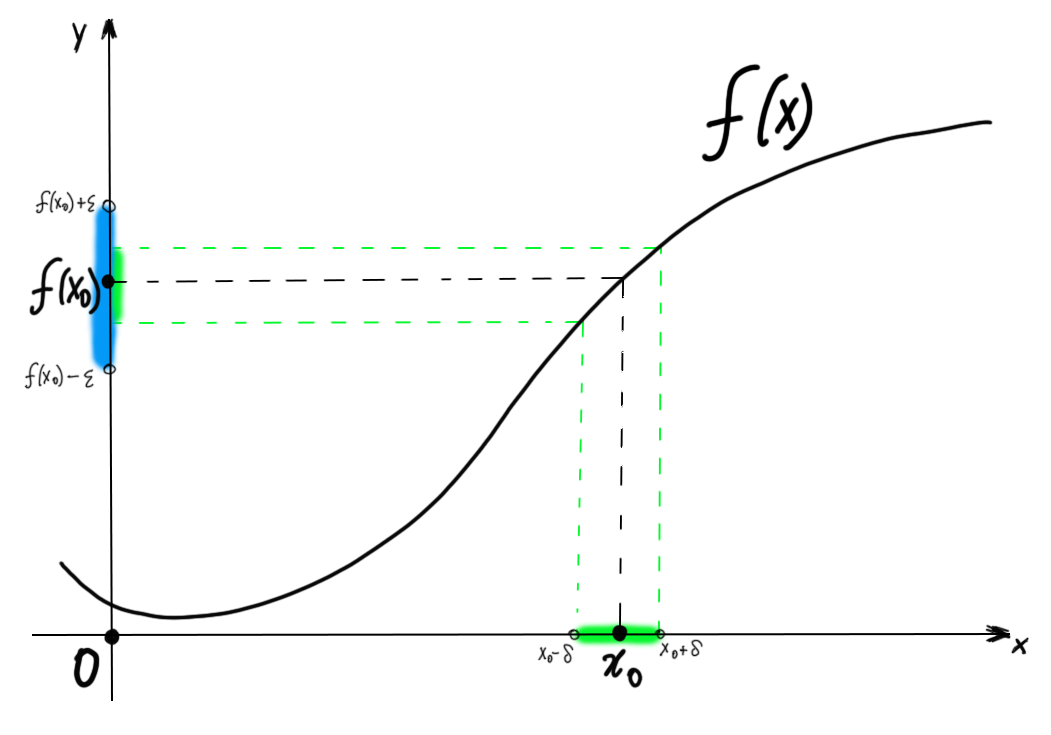
\includegraphics[width=0.7\linewidth]{images/continous.png}
    \caption{Пример графика непрерывной функции; для любой \textcolor{cyan}{$\varepsilon$-окрестности} точки $f(x_0)$ найдётся \textcolor{green}{$\delta$-окрестность} точки $x_0$, такая, что функция $f$ полностью отобразит эту \textcolor{green}{$\delta$-окрестность} в \textcolor{cyan}{$\varepsilon$-окрестность}.} 
    \label{fig:enter-label}
\end{figure}

\begin{proof}[Доказательство Леммы \ref{contious_on_R}]~

(1) Пусть $f:\mathbb{R} \to \mathbb{R}$ -- непрерывная функция, тогда она непрерывна в любой точке. Тогда для любой точки $x_0$ выполняются условия определения \ref{def_of_cont_on_sets_on_R}, а так как согласно Лемме \ref{interval_is_open} множества $\mathscr{B}_\delta(x_0), \mathscr{B}_\varepsilon(f(x_0))$ открыты, то мы получаем включение $f\bigl(\mathscr{B}_\delta(x_0) \bigr) \subseteq \mathscr{B}_\varepsilon(f(x_0)).$

(2) Пусть теперь в точке $x_0 \in \mathbb{R}$ и для любой $\varepsilon$-окрестности точки $f(x_0)$ всегда можно найти такую $\delta$-окрестность точки $x_0$, что $ f\bigl(\mathscr{B}_{\delta}(x_0) \bigr) \subseteq \mathscr{B}_{\varepsilon}(f(x_0))$. 

Рассмотрим теперь произвольную окрестность $\mathscr{W}(f(x_0))$ точки $f(x_0)$. Так как $\mathscr{W}(f(x_0))$ -- открытое в $\mathbb{R}$ множество, то согласно  определению \ref{open_in_R} существует такое $\varepsilon$-окрестность $\mathscr{B}_\varepsilon(f(x_0))$ точки $f(x_0)$, что $\mathscr{B}_\varepsilon(f(x_0)) \subseteq \mathscr{W}(f(x_0))$. Согласно предположению мы теперь можем найти $\delta$-окрестность точки $x_0$, что $ f\bigl(\mathscr{B}_{\delta}(x_0) \bigr) \subseteq \mathscr{B}_{\varepsilon}(f(x_0))$. Таким образом, мы получаем цепочку включений
\[
 f\bigl(\mathscr{B}_{\delta}(x_0) \bigr) \subseteq \mathscr{B}_{\varepsilon}(f(x_0)) \subseteq \mathscr{W}(f(x_0)),
\]
\textit{т.е.,} $f\bigl(\mathscr{B}_{\delta}(x_0) \bigr) \subseteq \mathscr{W}(f(x_0))$. Так как  (см. лемму \ref{interval_is_open}, $\mathscr{B}_{\delta}(x_0)$ -- открыто, то мы получаем, что для любого открытого множества $\mathscr{W}(f(x_0))$ мы нашли такое открытое $\mathscr{B}_{\delta}(x_0)$, что $f\bigl(\mathscr{B}_{\delta}(x_0) \bigr) \subseteq \mathscr{W}(f(x_0))$, а это и означает непрерывность (см. определение \ref{def_of_cont_on_sets_on_R}). Это завершает доказательство.
\end{proof}

\begin{corollary}\label{reform_of_cont}
  Для того, чтобы функция $f:\mathbb{R} \to \mathbb{R}$ была непрерывной в точке $x_0$, необходимо и достаточно, чтобы для всякого $\varepsilon>0$ существовал такой $\delta >0$, что из $|x-x_0|<\delta$ следует $|f(x)-f(x_0)|<\varepsilon$.    
\end{corollary}

\begin{proof}
    Действительно, для этого мы положим, что $\mathscr{W}(f(x_0)) = (f(x_0)-\varepsilon, f(x_0) + \varepsilon)$ и $\mathscr{U}(x_0) = (x_0-\delta,x_0 + \delta)$ в формулировке леммы \ref{contious_on_R}.
\end{proof}

\begin{figure}[h!]
    \centering
    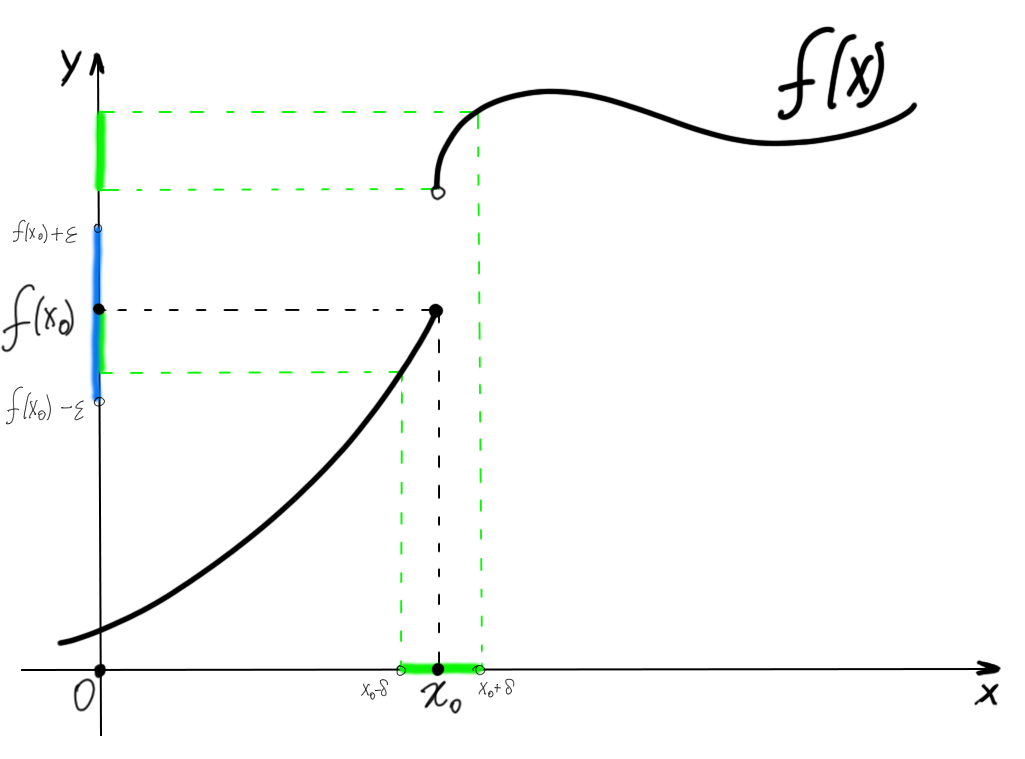
\includegraphics[width=0.7\linewidth]{images/non_continous.png}
    \caption{Пример графика функции которая не является непрерывной в точке $x_0$; мы нашли такую \textcolor{cyan}{$\varepsilon$-окрестность} точки $f(x_0)$, что никакая \textcolor{green}{$\delta$-окрестность} точки $x$ целиком не отображается в эту \textcolor{cyan}{$\varepsilon$-окрестность}.}
    \label{fig:enter-label}
\end{figure}

\begin{remark}\label{not_continous}
Тогда если $f:\mathbb{R} \to \mathbb{R}$ не является непрерывной функцией  в точке $x_0$, то можно найти такую $\varepsilon$-окрестность $\mathscr{B}_\varepsilon(f(x_0))$ точки $f(x_0)$, что не существует $\delta$-окрестности $\mathscr{B}_\delta(x_0)$ точки $x_0$, что $f(\mathscr{B}_\delta(x_0)) \not \subseteq \mathscr{B}_\varepsilon(f(x_0))$. 
\end{remark}



\begin{example}\label{x^2_is_continous}
    Пусть $f(x) = x^2$. Покажем, что эта функция непрерывна. Возьмём произвольную точку $x_0 \in \mathbb{R}$ и покажем, что $f$ непрерывна в этой точке. Согласно следствию \ref{reform_of_cont}, нам нужно для любого $\varepsilon>0$ найти такое $\delta >0$, что из неравенства $|x- x_0|< \delta$ будет следовать неравенство $|x^2 - x_0^2|<\varepsilon.$

    Имеем
    \begin{eqnarray*}
        |f(x)- f(x_0)| &=& |x^2 - x_0^2| \\
        &=& |(x-x_0)(x+x_0)| \\
        &=& |x-x_0| \cdot |x+x_0| \\
        &=& |x-x_0|\cdot \left| (x-x_0) + 2x_0 \right| \\
        &\le& |x-x_0| \cdot \left( |x-x_0| + 2 |x_0| \right).
    \end{eqnarray*}

Поэтому если $|x-x_0|<\delta$ и если мы потребуем, чтобы $\delta (\delta + 2|x_0|)<\varepsilon$, то из неравенства $|x-x_0|<\delta$ будет следовать неравенство $|f(x)- f(x_0)| < \varepsilon$, что и доказывает непрерывность этой функции. 
\end{example}

\begin{example}\label{x^2sin(1x)}
Покажем, что функция $f:\mathbb{R} \to \mathbb{R}$
    \[
    f(x) = \begin{cases}
         x^2 \sin \frac{1}{x}, & x \ne 0, \\
         0, & x =0
     \end{cases}
    \]
непрерывнa в точке $0$.

Это значит, что для любого $\varepsilon >0$ мы должны найти такую $\delta >0$, что из неравенства $|x|<\delta$ будет следовать $|{f}(x) - {f}(0)| = |f(x)| <\varepsilon.$

Имеем 
    \[
    \left|{f}(x) -{f}(0)\right| = \left|x^2 \sin \frac{1}{x} - 0 \right| = \left|x^2 \sin \frac{1}{x}\right| \le |x^2| = x^2,
    \]
поэтому если $x^2 <\varepsilon$, \ie $-\sqrt{ \varepsilon} <x < \sqrt{\varepsilon}$, то и $|{f}(x) - {f}(0)| <\varepsilon$. Значит, для любого $0 < \delta < \sqrt{\varepsilon}$ из неравенства $|x|<\delta$ вытекает неравенство $|{f}(x) - {f}(0)|$, что и доказывает непрерывность в точке $0.$
\end{example}

\subsection{Критерий непрерывности}


\begin{theorem}\label{preimage_of_open}
Пусть $X,Y \subseteq \mathbb{R}$ -- непустые подмножества на прямой. Функция $f:X \to Y$ непрерывна тогда и только тогда, когда прообраз любого открытого множества в $Y$ является открытым множеством в $X.$
\end{theorem}
\begin{proof}~

(1) Пусть $f:X \to Y$ -- непрерывная функция. Возьмём произвольное открытое множество $\mathscr{W} \subseteq Y$ и покажем, что множество $f^{-1}(\mathscr{W})$ открыто в $X$.

Пусть $x \in f^{-1}(\mathscr{W})$, тогда существует такой $y \in \mathscr{W}$, что $f(x) = y$. Далее, так как $\mathscr{W}$ является открытым множеством в $Y$, при этом $y\in \mathscr{W}$, $f(x) = y$, и $f$ -- непрерывно в $x$, то согласно определению \ref{def_of_cont_on_sets_on_R}, найдётся такое открытое в $X$ множество $\mathscr{U} \subseteq X$, что $x \in \mathscr{U}$ и $f(\mathscr{U}) \subseteq \mathscr{W}.$ Тогда согласно предложению \ref{good_for_maps}, получаем включение
\[
 f^{-1}(f(\mathscr{U})) \subseteq f^{-1}(\mathscr{W}),
\]
наконец, согласно предложению \ref{good_for_preimage}, имеем
\[
 \mathscr{U} \subseteq f^{-1}(f(\mathscr{U})) \subseteq f^{-1}(\mathscr{W}).
\]

Итак, мы получили следующее. Для любой точки $x \in f^{-1}(\mathscr{W})$ мы нашли такое открытое в $X$ множество $\mathscr{U}$, что

\[
 x \in \mathscr{U} \subseteq f^{-1}(f(\mathscr{U})) \subseteq f^{-1}(\mathscr{W}).
\]
но тогда согласно предложению \ref{open_via_open} множество $f^{-1}(\mathscr{W})$ -- открыто в $X.$


(2) Пусть прообраз любого открытого множества в $Y$ есть открытое множество в $X$. Пусть $f(x) = y$ и пусть $y \in \mathscr{W}$, где $\mathscr{W}$ -- открытое множество в $Y$. Тогда $x \in f^{-1}(\mathscr{W})$, а так как мы предположили, что множество $f^{-1}(\mathscr{W})$ -- открыто в $X$, то согласно предложению \ref{open_via_open}, найдётся такое открытое множество $\mathscr{U}$ в $X$, что
\[
 x \in \mathscr{U} \subseteq f^{-1}(\mathscr{W}).
\]

Так как $\mathscr{U} \subseteq f^{-1}(\mathscr{W})$, то согласно предложению \ref{good_for_maps}, имеем $f(\mathscr{U}) \subseteq f(f^{-1}(\mathscr{W}))$. Наконец, согласно предложению \ref{good_for_preimage}, $f(f^{-1}(\mathscr{W})) \subseteq \mathscr{W}$.

Итак, мы получили, что для любой точки $y\in Y$ и любого открытого множества $\mathscr{W}$ в $Y$ мы нашли такое открытое множество $\mathscr{U}$ в $X$, что 
\[
f(\mathscr{U}) \subseteq f(f^{-1}(\mathscr{W})) \subseteq \mathscr{W},
\]
\textit{т.е.} $f(\mathscr{U}) \subseteq \mathscr{W}$, но согласно определению \ref{def_of_cont_on_sets_on_R}, это и означает непрерывность в точке $x$, а так как $x$ -- произвольная точка, то это означает непрерывность на всём $X$.
\end{proof}

\begin{mydangerr}{\bf!}
    Следует заметить, что образ открытого множества при непрерывном отображении, вообще говоря, \textbf{не будет} открытым множеством.
\end{mydangerr}


\begin{example}
    Вернёмся к примеру \ref{x^2_is_continous}, $f:\mathbb{R} \to \mathbb{R}$, $f(x) = x^2$. Мы показали, что $f$ -- непрерывная функция. Если мы рассмотрим теперь открытый интервал $(-1,1)$, то его образом при $f$ будет множество $[0,1)$, которое не открыто в $\mathbb{R}$ (см. Пример \ref{(a,b)c(open}).
\end{example}



\begin{theorem}\label{comp_of_continous_on_R}
 Пусть $X,Y,Z \subseteq \mathbb{R}$ -- непустые подмножества  и пусть $f:X \to Y$, $g:Y \to Z$ -- функции.
\[
 \xymatrix{
 X \ar@{->}[r]^f \ar@{->}[rd]_{g\circ f} & Y \ar@{->}[d]^g \\
 & Z 
 }
\]
Если $f$ непрерывная в точке $x_0$ и $g$ непрерывная в точке $f(x_0)$, то функция $h = g \circ f$ непрерывная в точке $x_0.$ Если $f$ непрерывна на всём $X$ и $g$ непрерывная на всём $Y$, то $h$ непрерывная на всём $X.$
\end{theorem}
 \begin{proof}
Пусть $\mathscr{W}$ -- окрестность точки $h(x_0) =  g(f(x_0))$. Тогда из предположения о непрерывности (см. Определение \ref{def_of_cont_on_sets_on_R}) найдётся окрестность $\mathscr{V}$ точки $f(x_0)$, такая что
\[
 g(\mathscr{V}) \subseteq \mathscr{W}.
\]

С другой стороны, так как $f$ -- непрерывна в точке $x_0$, тогда (см. Определение \ref{def_of_cont_on_sets_on_R}) для этой же окрестности $\mathscr{V}$ существует окрестность $\mathscr{U}$ точки $x_0$, такая что
\[
 f(\mathscr{U}) \subseteq \mathscr{V}.
\]

Воспользовавшись теперь (\ref{A<B->F(A)<F(B)}), мы получаем 
\[
 g(f(\mathscr{U})) \subseteq g(\mathscr{V)} \subseteq \mathscr{W},
\]
но это и означает (см. Определение \ref{def_of_cont_on_sets_on_R}) что функция $h = g \circ f$ -- непрерывна в точке $x_0$.

Второе утверждение, очевидно, следует из первого. 
 \end{proof}


\begin{corollary}\label{restriction_on_R}
    Если $f:X \to Y$ непрерывное в точке $x_0$ функция, и $A \subseteq X$, $A \ni x_0$, то сужение $f|_A:=f \circ \mathrm{in}_A$ также непрерывно в $x_0,$ где $\mathrm{in}_A:A \hookrightarrow X$ -- вложение.
\end{corollary}
\begin{proof}
    На самом деле, $f$ непрерывно в $x_0$ по условию, а $\mathrm{in}_A$ непрерывно в любой точке $a \in A$ (потому что это тождественная функция), тогда из предыдущей теоремы и следует утверждение.
\end{proof}




\section{Лекция \#13. Пределы}

\subsection{Основное определение}

\begin{definition}\label{the_main_def_of_limit_on_R}
Пусть $X, Y \subseteq \mathbb{R}$ -- непустые подмножества, $x_0 \notin X$, но $x_0 \in \overline{X}$. Пусть далее $f: X \to Y$. Мы будем говорить, что $f(x)$ \textit{имеет предел $y_0 \in Y$ при $x \in X$, стремящемся к $x_0$ (или $y_0$ есть предел функции $f$ в точке $x_0 \in \overline{X}$ по множеству $X$}), если функция $\overline{f}:X \cup \{x_0\} \to Y$, определённая условиями
    \[
     \overline{f}(x) = \begin{cases}
         f(x), & x \in X, \\
         y_0, & x = x_0,
     \end{cases}
    \]
    непрерывна в точке $x_0$.
\end{definition}

В этом случае, мы пишем
\[
 y_0 := \lim_{x\to x_0, x \in X} f(x).
\]

\begin{mydanger}{\bf{!}}
    Если $x_0 \in X$, то мы пользуемся той же терминологией и теми же обозначениями как и в случае, когда функция $f$ непрерывна в точке $x_0$, причём $y_0:=f(x_0).$
\end{mydanger}

\begin{example}
Пусть $X = \mathbb{R}\setminus\{0\}$, $Y = \mathbb{R}$, а функция $f:X\to Y$ задана следующим образом:
\[
 f(x): = x^2 \sin \frac{1}{x}.
\]

\begin{figure}[h!]
    \centering
    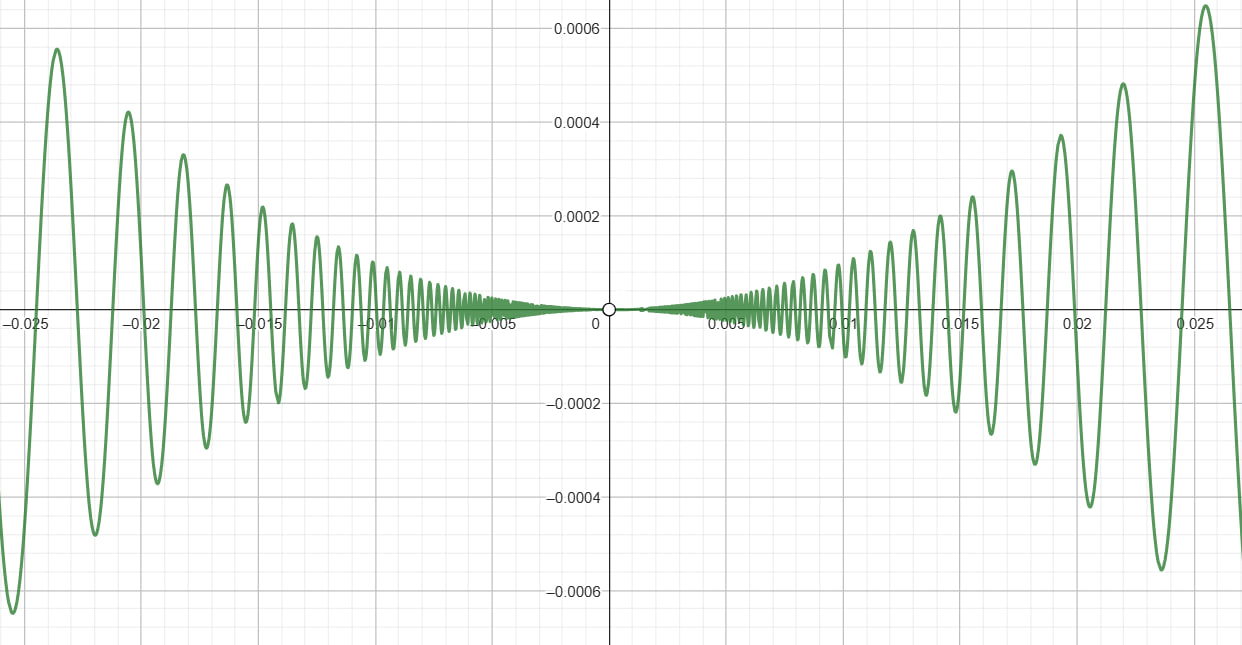
\includegraphics[width=1\linewidth]{images/x2sin.jpg}
    \caption{График функции $f(x) = x^2 \sin \frac{1}{x}$. Видно, что если мы положим $f(0):=0$, то мы получим непрерывную функцию на всей прямой $\mathbb{R}$.}
\end{figure}


Ясно, что любая окрестность точки $x_0=0$ пересекается с множеством $X$, поэтому точка $x_0 = 0$ -- точка прикосновения для множества $X$, \textit{т.е.} $0 \in \overline{X}$.

Продолжим теперь нашу функцию на множестве $X\cup \{0\}$ следующим образом:
    \[
    \overline{f}(x) = \begin{cases}
         x^2 \sin \frac{1}{x}, & x \ne 0, \\
         0, & x =0
     \end{cases}
    \]
и покажем, что она непрерывнa в точке $x_0 =0$.

Это значит, что для любого $\varepsilon >0$ мы должны найти такую $\delta >0$, что из неравенства $|x|<\delta$ будет следовать $|\overline{f}(x) -\overline{f}(0)| = |\overline{f}(x)| <\varepsilon.$

Имеем 
    \[
    \left|\overline{f}(x) -\overline{f}(0)\right| = \left|x^2 \sin \frac{1}{x} - 0 \right| = \left|x^2 \sin \frac{1}{x}\right| \le |x^2| = x^2,
    \]
поэтому если $x^2 <\varepsilon$, \ie $-\sqrt{ \varepsilon} <x < \sqrt{\varepsilon}$, то и $|\overline{f}(x) - \overline{f}(0)| <\varepsilon$. Значит, для любого $0 < \delta < \sqrt{\varepsilon}$ из неравенства $|x|<\delta$ вытекает неравенство $|\overline{f}(x) - \overline{f}(0)|$, что и доказывает непрерывность в точке $0.$ 

Поэтому имеем
\[
\lim_{x \to 0, x \in X}f(x) = 0  
\]
\begin{flushright}
    $\square$
\end{flushright}
\end{example}


Вспомнив определение непрерывности (см. Определение \ref{def_of_cont_on_sets_on_R}) и точки прикосновения (см. Определение \ref{limit_point}), определение предела можно переформулировать следующими двумя эквивалентными способами:

\begin{definition}\label{lim_via_neighberhoods}
Когда говорят, что функция $f: X \to Y$ имеет предел $y_0$ при $x \in X$, стремящимся к $x_0$, и при этом пишут
\[
 \lim_{x \to x_0, x \in X}f(x) = y_0
\]
то это означает, что для каждого открытого в $Y$ множества $\mathscr{W}$, $y_0 \in \mathscr{W}$ найдётся такое открытое в $\mathbb{R}$ множество $\mathscr{U}$, что $x_0 \in \mathscr{U}$ и $f(\mathscr{U}\cap X) \subseteq \mathscr{W}$. 
\end{definition}

\begin{mydanger}{\bf{!}}
    Так как $x_0 \in \overline{X}$, то множество $X \cap \mathscr{U}$ никогда не пусто.
\end{mydanger}

\begin{definition}\label{def_for_cont_via_d-e_on_R}
Сказать, что функция $f: X \to Y$ имеет предел $y_0$ при $x \in X$, стремящимся к $x_0$, и при этом написать
\[
 \lim_{x \to x_0, x \in X}f(x) = y_0,
\]
это то же самое, что сказать, что для каждого $\varepsilon>0$ можно найти такое $\delta >0$, что из $x \in X$ и $|x-x_0|<\delta$ следует $|f(x) - f(x_0)|<\varepsilon.$
\end{definition}

\begin{proposition}
 Функция может иметь лишь один предел по множеству $X$ в данной точке $x_0 \in \overline{X}.$
\end{proposition}
\begin{proof}
    Пусть  $\lim_{x \to x_0, x \in X}f(x) = y_0$ и $\lim_{x \to x_0, x \in X}f(x) = y_0'$, при этом $y_0 \ne y_0'$. Тогда согласно Определению \ref{def_for_cont_via_d-e_on_R}, мы для любого $\varepsilon>0$ можем найти такие $\delta, \delta' >0$, что из неравенств $|x-x_0|< \delta$, $|x-x_0|<\delta'$ будут следовать неравенства $|f(x) - y_0|, |f(x)-y_0'|<\varepsilon.$

Имеем
\begin{eqnarray*}
    |y_0 - y_0'| &=& |y_0 - f(x) + f(x) - y_0'| \\
    &=& |(y_0-f(x)) + (f(x) - y_0')| \\
    &\le & |f(x) - y_0| + |f(x) - y_0'| \\
    &<& 2 \varepsilon,
\end{eqnarray*}
\textit{т.е.} расстояние между фиксированными точками $y_0,y_0' \in Y$ может быть любым, что невозможно, если $y_0 \ne y_0'.$
\end{proof}





\subsection{Критерий непрерывности в терминах предела}

Из определения предела вытекает:

\begin{theorem}[{Критерий непрерывности}]\label{criteria_of_continous}
Функция $f: X \to Y$ непрерывна в точке $x_0 \in X$, являющейся точкой прикосновения множества $X\setminus\{x_0\}$, тогда и только тогда, когда
\[
f(x_0) = \lim_{x \to x_0, x\in X \setminus \{x_0\}}f(x)
\]
\end{theorem}
\begin{proof}
    Это лишь пересказ определения предела (см. Определение \ref{the_main_def_of_limit_on_R}).
\end{proof}

\begin{theorem}\label{limit_for_any_subset}
    Пусть $y_0 = \lim_{x \to x_0, x \in X} f(x)$. Тогда для каждого подмножества $A \subseteq X$, для которого $x_0 \in \overline{A}$, $y_0 = \lim_{x \to x_0, x \in B}f(x)$.
\end{theorem}

\begin{proof}
    Это сразу следует из определения предела (см. Определение \ref{the_main_def_of_limit_on_R}) и следствия \ref{restriction_on_R}.
\end{proof}





\begin{theorem}\label{lim_of_composition_on_R}
Пусть $X,Y,Z \subseteq \mathbb{R}$ -- непустые множества, пусть имеем функции 
\[
 \xymatrix{
 X \ar@{->}[r]^f \ar@{->}[rd]_{g\circ f} & Y \ar@{->}[d]^g \\
 & Z
 }
\]
Тогда, если
\[
 \lim_{x\to x_0, x\in X}f(x) = y_0,
\]
и функция $g$ -- непрерывна в точке $y_0$, то
\[
 g(y_0) = \lim_{x \to x_0, x \in X} (g \circ f)(x).
\]     
\end{theorem}
\begin{proof}
    Это сразу следует из определения предела (см. Определение \ref{the_main_def_of_limit_on_R}) и теоремы \ref{comp_of_continous_on_R}.
\end{proof}

\begin{mydanger}{\bf{!}}
    В случае, когда $X = \mathbb{R}$, мы будем вместо $\lim_{x \to x_0, x \in \mathbb{R}}f(x)$ писать $\lim_{x \to x_0}f(x).$
\end{mydanger}


\subsection{Окрестность бесконечности}\label{neighborhood_of_infinity}

Мы сейчас довольно-таки ``окольным путём'' приблизимся к понятию гомеоморфизма между топологическими пространствами. Делаем мы это лишь для того, чтобы не перегрузить читателя большим количеством новых терминов, которые потом не будут так часто использоваться.

\begin{construction}\label{con_of_induced_topology}
 Пусть дано некоторое непустое подмножество $X\subseteq \mathbb{R}$ и произвольное множество $S$. Допустим, что у нас есть биекция $\varphi:X \to S$, тогда мы можем снабдить это абстрактное множество $S$ топологией, наследованной из множества $X$, а именно будем считать $\mathscr{V} \subseteq S$ открытым тогда и только тогда, когда $\varphi^{-1}(\mathscr{V}) \subseteq X$ -- открыто в $X.$
\end{construction}

\begin{mydangerr}{\bf !}
    Если рассматривать абстрактные топологические пространства, то в таком случае непрерывное отображение между ними определяют как такое отображение, прообраз каждого подмножества которого открыт. Фактически, то что мы определили, это специально построили такую топологию на $S$, чтобы $\varphi$ было непрерывным.
\end{mydangerr}


\begin{definition}
 Обозначим через $\overline{\mathbb{R}}$ множество, являющееся объединением $\mathbb{R}$ и двух новых элементов, обозначаемых символами $+\infty$ и $-\infty$ (=\textit{бесконечные точки}), \textit{т.е}
\[
 \overline{\mathbb{R}}: = \mathbb{R}\cup \{-\infty\} \cup \{+\infty\}.
\]
\end{definition}

\begin{mydanger}{\bf !}
Об этих символах следует думать как о бесконечно удалённых точках. Самый более или менее подходящий пример — это понятие горизонта, которого никогда не достигнуть.
\end{mydanger}

\begin{figure}
    \centering
    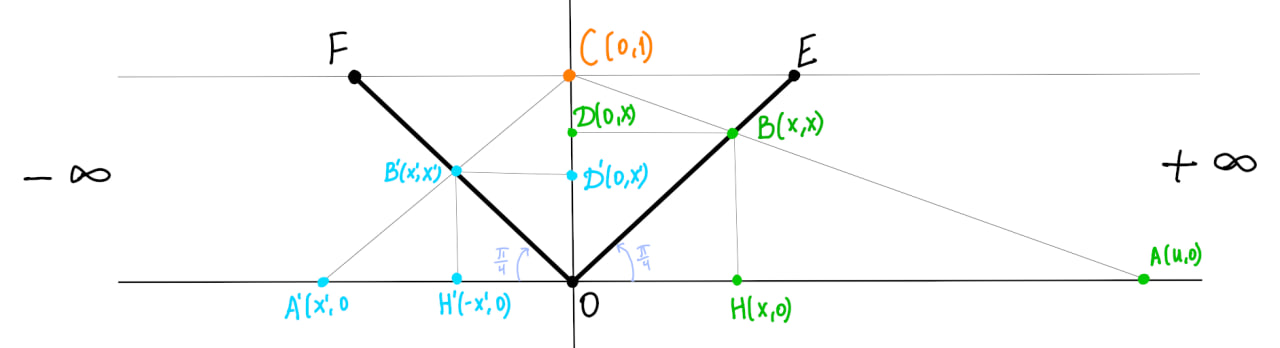
\includegraphics[width=1\linewidth]{images/infty.jpg}
    \caption{Схема отображения $\varphi: [-1,1] \to \overline{R}$; сам отрезок $[-1,1]$ тут представлен ломаной $FOE$. Тонкие линии на рисунке показывают, куда отображаются точки отрезка; $E \mapsto +\infty$, $B \mapsto A$, $B' \mapsto A'$, $F \mapsto -\infty$. Ясно, что это биекция.}
    \label{infnty_picture}
\end{figure}

Наша цель — это ввести топологию на множестве $\overline{\mathbb{R}}$. Мы будем делать это исходя из того, что мы знаем топологию на отрезке. Для этого нам понадобится биекция $\varphi: [-1,1] \to \overline{\mathbb{R}}$ и Конструкция \ref{con_of_induced_topology}.

Напомним (см. Теорема \ref{open_in_K}), что открытые множества в $[-1,1]$ это множества вида $\mathscr{U} \cap [-1,1]$, тогда, например, окрестностью точки $1$ будет множество $(\alpha, 1]$, где $-1 \le \alpha<1$.

\begin{construction}\label{construction_of_bijection}
Определим отображение $\varphi: [-1,1] \to \overline{\mathbb{R}}$, следующим образом
\[
 \varphi(x): = \begin{cases}
     \frac{x}{1-|x|}, & -1<x<1,\\
     + \infty, &x = 1, \\
     -\infty, & x=-1
 \end{cases}
\]
схема которого изображена на Рис.\ref{infnty_picture}. Обратное отображение $\varphi^{-1}: \overline{\mathbb{R}} \to [-1,1]$ выглядит следующим образом
\[
\varphi^{-1}(x): = \begin{cases}
    \frac{x}{1+ |x|}, & x \in \mathbb{R},\\
    1, & x = + \infty,\\
    -1, & x = - \infty.
\end{cases}
\]
\end{construction}

\begin{lemma}\label{x<y->f(x)<f(x)}
    Если $x,y\in \mathbb{R}$, то $x\le y$ тогда и только тогда, когда $\varphi^{-1}(x) \le \varphi^{-1}(y)$.
\end{lemma}
\begin{proof}
Рассмотрим все возможные случаи.

(1) Пусть $x,y \ge 0$, тогда $|x| =x$ и $|y| = y$.

Имеем
\begin{eqnarray*}
    x \le y &\Longleftrightarrow& x+ xy \le y + xy \\
    & \Longleftrightarrow& x (1 + y) \le y(1 + x)\\
    &\Longleftrightarrow& x(1+ |y|) \le y (1+ |x|)\\
    &\Longleftrightarrow& \frac{x}{1+|x|} \le \frac{y}{1+|y|}\\
    &\Longleftrightarrow& \varphi^{-1}(x) \le \varphi^{-1}(y).
\end{eqnarray*}

(2) Пусть $x <0$, $y \le 0$, тогда $|x|  =- x$ и $|y| = y$, а также $xy < 0$.

Имеем

\begin{eqnarray*}
    x \le y &\Longleftrightarrow& x + xy \le  y+xy \le y -xy \\
    &\Longleftrightarrow& x+xy \le y - xy\\
    &\Longleftrightarrow& x(1+y) \le y(1-x) \\
    &\Longleftrightarrow& \frac{x}{1-x} \le \frac{y}{1+y}\\
    &\Longleftrightarrow& \varphi^{-1}(x) \le \varphi^{-1}(y).
\end{eqnarray*}

(3) Пусть $x,y < 0$ и $x\le y$, тогда $|x| = -x$, $|y| = -y$, $xy >0$.

Имеем

\begin{eqnarray*}
    x \le y &\Longleftrightarrow& x-xy \le y - xy \\
    &\Longleftrightarrow & x(1-y) \le y(1-x) \\
    &\Longleftrightarrow& \frac{x}{1-x} \le \frac{y}{1-y}\\
    &\Longleftrightarrow& \frac{x}{1+|x|} \le \frac{y}{1+ |y|} \\
     &\Longleftrightarrow& \varphi^{-1}(x) \le \varphi^{-1}(y).
\end{eqnarray*}

Это завершает доказательство.
\end{proof}

\begin{construction}
 На $\overline{\mathbb{R}}$ введём отношение порядка, по определению считая неравенство $x \le y$ эквивалентным неравенству $\varphi^{-1}(x) \le \varphi^{-1}(y)$. Легко проверить, что, когда $x,y \in \mathbb{R}$, это отношение порядка есть обычное отношение порядка на $\mathbb{R}$ и что, кроме того, для любого $x\in \mathbb{R}$ мы имеем $- \infty < x < \infty.$    
\end{construction}

\begin{mydanger}{\bf !}
    Действительные числа называются также \textit{конечными} элементами $\overline{\mathbb{R}}.$ 
\end{mydanger}~

Таким образом, согласно конструкции \ref{con_of_induced_topology} и теореме \ref{open_in_K}, получаем следующее

\begin{definition}
 Открытые множества в $\overline{R}$ — это открытые множества $\mathbb{R}$, а также множества вида $\varphi(\mathscr{U}\cap [-1,1])$, таким образом, окрестностями точек $-\infty,+\infty$ могут служить, например, множества $[-\infty, a)$, $(b,+\infty]$, соответственно, где $a,b \in \mathbb{R}$.  
\end{definition}


\begin{lemma}\label{niegh_of_infty_on_R}
  Точки $-\infty, + \infty$ -- точки прикосновения для $\mathbb{R} \subseteq \overline{\mathbb{R}}.$
 \end{lemma}
 \begin{proof}
Мы докажем это утверждение для $+\infty$, так как для $-\infty$ оно доказывается аналогично.

Итак, пусть $\mathscr{W}$ -- окрестность точки $+\infty$, тогда, согласно конструкциям \ref{con_of_induced_topology}, \ref{construction_of_bijection}, существует открытое в $[-1,1]$ множество $\mathscr{U}(1)$, содержащее точку $1$, такое, что $\mathscr{W} = \varphi^{-1}(\mathscr{U}(1))$.  

Но, согласно определению \ref{e-neigh_in_A}, множество $\mathscr{U}(1)$ содержит в себе множество вида $(a,1]$, где $-1\le a <1$. Далее, согласно свойству (\ref{A<B->F(A)<F(B)}), получаем, 
\[
 (a,1] \subseteq \mathscr{U}(1) \Longrightarrow \varphi((a,1]) \subseteq \varphi(\mathscr{U}(1)) = \mathscr{W},
\]
наконец, согласно конструкции \ref{construction_of_bijection} и лемме \ref{x<y->f(x)<f(x)}, получаем
\[
 \varphi((a,1]) = \left.\left( \frac{a}{1-|a|}, +\infty\right.\right],
\]
\textit{т.е.} $\left.\left( a', +\infty\right.\right] \subseteq \mathscr{W}$, где $a' = \frac{a}{1-|a|}$. Итак, любая окрестность точки $+\infty$ содержит в себе множество вида $(a',\infty]$, где $a' \in \mathbb{R}$. Но так как $(a',\infty] \cap \mathbb{R} \ne \varnothing$, то это и означает, что $+\infty$ -- точка прикосновения. 
 \end{proof}

\subsection{Символ $\lim\limits_{x \to \infty}$ и предел последовательности}

Пусть теперь $X,Y \subseteq \overline{\mathbb{R}}$ -- непустые подмножества и пусть $f: X \to Y$ -- функция. 

\begin{remark}\label{about_infty}
Так как (см. Лемму \ref{niegh_of_infty_on_R}) любая окрестность точки $+\infty$ (\textit{соотв.} точки $-\infty$) содержит в себе множество $(a,+\infty]$ (\textit{соотв.} множество $[-\infty, a)$), то получаем
\begin{enumerate}
    \item[] во-первых, если $+\infty$ (\textit{соотв.} $-\infty$) -- точка прикосновения для $X$, то это значит что для любого $x \in X$ существует, такой $x' \in X$, что $x<x'$ (\textit{соотв.} $x'<x$),
    \item[] во-вторых, если $f$ -- непрерывна в точке $-\infty$, то это значит, что для любого открытого в $Y$ множества $\mathscr{W}(y_0)$, содержащее точку $y_0 = f(-\infty)$ найдётся такое число $a \in X$, что для всех $x'\in X$, с условием $x'< a$ верно то, что $f(x') \in \mathscr{W}(y_0)$,
    \item[] аналогично, если $f$ -- непрерывна в точке $+\infty$, то это значит, что для любого открытого в $Y$ множества $\mathscr{W}(y_0)$, содержащее точку $y_0 = f(+\infty)$ найдётся такое число $a \in X$, что для всех $x'\in X$, с условием $x'>a$ верно то, что $f(x') \in \mathscr{W}(y_0)$.
\end{enumerate}    
\end{remark}


Рассмотрим теперь множество натуральных чисел $\mathbb{N} \subseteq \mathbb{R}$, тогда, согласно теореме \ref{open_in_K}, любое открытое в $\mathbb{N}$ множество это множество вида $\mathscr{U} \cap \mathbb{N}$.

Это значит, что все натуральные числа в любом открытом множестве $\mathscr{U} \subseteq \mathbb{R}$ и есть открытое множество в $\mathbb{N}$, \textit{т.е.,} любой набор точек из $\mathbb{N}$ образует открытое множество в $\mathbb{N}$. В частности одноточечное множество $\{n\}$ -- открыто в $\mathbb{N}.$

\begin{mydangerr}{\bf !}
    Аналогично рассуждая (используя предложение \ref{closed_in_A_if}), получаем что любой набор точек из $\mathbb{N}$ -- замкнут. Таким образом, в $\mathbb{N}$ любое подмножество как замкнуто так и открыто одновременно и более того, любая точка тоже обладает этим свойством. 
\end{mydangerr}

\begin{theorem}\label{lim_of_seqence=contionous}
 Пусть дана последовательность $(x_n)$ каких-то элементов множества $X \subseteq \mathbb{R}$ и пусть $\lim_{n\to \infty}x_n =a$ в смысле определения \ref{limit_of_seqeunce}, тогда функция $\m{x}: \mathbb{N} \to X$ определённая условием
    \[
     \m{x}(n): =\begin{cases}
         x_n, & n \ge 1\\
         a, & n = +\infty
     \end{cases}
    \]
    непрерывна в точке $+\infty$, а значит $\lim_{n \to +\infty\, n \in \mathbb{N}}\m{x}(n) = a$ в смысле определения \ref{the_main_def_of_limit_on_R}. И более того, верно и обратное утверждение.
\end{theorem}
\begin{proof}
    Это сразу следуют из определения \ref{limit_of_seqeunce}, определения \ref{the_main_def_of_limit_on_R} и замечания \ref{about_infty}.
\end{proof}





\section{Лекция \#14. Определение предела в терминах предал последовательностей и $o$-символика}

\subsection{Предел функции в терминах предела последовательностей}

Мы сейчас выведем ещё одно очень полезное свойство предела функции, которое принято называть \textit{определением предела функции по Гейне\footnote{Генрих Эдуард Гейне (нем. Heinrich Eduard Heine; 15 марта 1821, Берлин, Германия — 21 октября 1881, Галле, Германия) — немецкий математик, профессор. Ученик Дирихле.}}.

\begin{lemma}\label{choice_of_seqeunce_on_R}
Пусть $A\subseteq \mathbb{R}$ -- непустое множество, тогда для любой точки $a \in \overline{A}$ существует такая последовательность $(a_n)$ точек из $A$, что $a = \lim_{n \to \infty} a_n$.
\end{lemma}

\begin{proof}
 Так как $a$ -- точка прикосновения, то для любой её $\varepsilon$-окрестности $(a-\varepsilon, a+\varepsilon)$ имеем $A \cap (a-\varepsilon, a+\varepsilon) \ne \varnothing$. Другими словами любая её $\varepsilon$-окрестность $(a-\varepsilon, a+\varepsilon)$ содержит хотя бы одну точку из $A$. В частности,  для любого $n\ge 1$, пологая $\varepsilon: = \frac{1}{n}$, получаем 
 \[
  \left(a - \frac{1}{n}, a+ \frac{1}{n} \right) \cap A \ne \varnothing.
 \]

Тогда для каждого $n\ge 1$ мы можем выбрать\footnote{так как у нас счётный набор множество, то это можно сделать не прибегая к помощи аксиомы выбора.} $a_n \in   \left(a - \frac{1}{n}, a+ \frac{1}{n} \right) \cap A$.

Покажем, что $\lim_{n \to \infty} a_n = a$. Действительно, пусть $n<m$, и мы имеем тогда 
\[
 a_n \in   \left(a - \frac{1}{n}, a+ \frac{1}{n} \right) \cap A \mbox{ и } a_m \in   \left(a - \frac{1}{m}, a+ \frac{1}{m} \right) \cap A.
\]

Получаем
\begin{eqnarray*}
    |a_n -a_m| &=& |a_n - a + a - a_m| \\
    &=& |(a_n -a) + (a - a_m)| \\
    &\le & |a_n - a| + |a- a_m| \\
    &<& \frac{1}{n} + \frac{1}{m} < \frac{2}{n}.
\end{eqnarray*}

Это означает, что все $a_n, a_{n+1}, \ldots \in \left(a-\frac{2}{n}, a+ \frac{2}{n}\right)$, \textit{т.е.,} последовательность $(a_n)$ -- фундаментальная (см. Определение \ref{foundamental_sequence}), а тогда согласно критерию Коши (см. Теорема \ref{Coshy}), $\lim_{n \to \infty} a_n = a.$ Это завершает доказательство.
\end{proof}

Следующий результат некоторые авторы принимают за определение предела функции, и говорят, что это определение функции по Гейне.

\begin{theorem}\label{lim=>for_any_sequence}
 Пусть $X,Y \subseteq \mathbb{R}$ -- непустые множества, $f: X \to Y$ -- функция, и $x_0 \in \overline{X}.$ Для того, чтобы $f$ имело предел $y_0 \in Y$ в точке $x_0$ по $X$, необходимо и достаточно, чтобы для каждой последовательности $(x_n)$ точек из $X$, сходящейся к $x_0$, последовательность $(f(x_n))$ сходилась к $y_0.$
\end{theorem}

\begin{proof}~

(1) Пусть $\lim_{x \to x_0, x \in X}f(x) = y_0$, тогда согласно определению предела \ref{the_main_def_of_limit}, функция $\overline{f}: X \cup \{x_0\} \to \mathbb{R}$,
\[
 \overline{f}(x) = \begin{cases}
     f(x), & x \ne x_0 \\
     y_0, & x = x_0
 \end{cases}
\]
является непрерывной в точке $x_0$.

Далее, так как $x_0 \in \overline{X}$, то согласно лемме \ref{choice_of_seqeunce_on_R}, мы можем выбрать такую последовательность $(x_n)$ точек из $X$, такая что $\lim_{n \to \infty }x_n = x_0$. Далее, согласно теореме \ref{lim_of_seqence=contionous}, функция $\m{x}: \mathbb{N} \to X$ определённая условиями
\[
 \m{x}(n): = \begin{cases}
     x_n, & n \ge 1,\\
     x_0, & n = +\infty
 \end{cases}
\]
-- непрерывна в точке $+\infty$, а значит и $\lim_{n \to +\infty,\, n \in \mathbb{N}}\m{x} = x_0$.

Итак, мы получаем коммутативную диаграмму
\[
 \xymatrix{
 \mathbb{N} \ar@{->}[r]^{\m{x}} \ar@{->}[rd]_{f \circ \m{x}} & X \ar@{->}[d]^f\\
 & Y
 }
\]
из которой видно, что функция $f\circ \m{x}$ это последовательность $(f(x_n))$, так как
\[
 (f\circ \m{x})(n):= f(\m{x}(n)) = f(x_n), \qquad n \ge 1.
\]

Более того по Теореме \ref{lim_of_composition_on_R}, эта последовательность $(f(x_n))$ имеет предел $y_0 = \overline{f}(x_0)$, что и доказывает необходимость.

(2) Будем доказывать от противного. Пусть для любой последовательности $(x_n)$ точек из $X$, $\lim_{n \to \infty} x_n = x_0$ имеем $\lim_{n \to \infty}f(x_n) = y_0$, но $y_0 \ne \lim_{x \to x_0, x\in X}f(x)$ в смысле определения \ref{the_main_def_of_limit_on_R}.

Тогда поучаем, что
\begin{enumerate}
    \item[] с одной стороны, $\lim_{n \to \infty} x_n = x_0$ влечёт (см. Определение \ref{lim_of_composition}), что, начиная с какого-то номера $N$, $|x_n - x_0| < \varepsilon$ для всех $n > N$,
    \item[] а с другой стороны $\lim_{x \to x_0, x\in X}f(x) \ne y_0$ означает, что $f(x)$ не является непрерывный в точке $x_0$.
\end{enumerate}

Из последнего тогда получаем, что существует такое $\varepsilon >0$, что для любого номера $n$ найдётся такая точка $x_n \in X$, удовлетворяющая двум условиям:
\[
  |x_n - x_0| < \frac{1}{n}, \mbox{ и } |f(x_n) - y_0| \ge \varepsilon
\]

Но тогда последовательность $(f(x_n))$ не сходится к $y_0 = f(x_0)$, что противоречит условию.
\end{proof}

Используя теперь эту теорему мы легко доказываем следующий результат


\begin{theorem}\label{lim(f+g)}
Пусть даны три функции $f,g,h: X \to Y$, где $X,Y \subseteq \mathbb{R}$ -- непустые множества. И пусть
\[
 \lim_{x\to x_0, x \in X} f(x) = f(x_0),\quad  \lim_{x\to x_0, x \in X} g(x) = g(x_0),
\]
тогда верны следующие свойства, если они имеют смысл
\begin{enumerate}
     \item $\lim\limits_{x \to x_0, x \in X}(\alpha \cdot f(x)) = \alpha \cdot f(x_0),$
    \item $\lim\limits_{x\to x_0, x \in X} (f(x)+  g(x)) =  f(x_0) +  g(x),$
    \item $\lim\limits_{x\to x_0, x \in X} (f(x)\cdot g(x)) = f(x_0)\cdot g(x_0),$
    \item $\lim\limits_{x\to x_0, x \in X} \frac{1}{f(x)} = \frac{1}{f(x_0)},$
    \item Если $f(x) \le h(x) \le g(x)$ для всех $x\in X$, и $ \lim\limits_{x\to x_0, x \in X} f(x) =  \lim\limits_{x\to x_0, x \in X} g(x) = y_0$, то и $ \lim\limits_{x\to x_0, x \in X} h(x) = y_0$.
    \item Если $f(x) \le g(x)$ для всех $x \in X$, то $ \lim\limits_{x\to x_0, x \in X} f(x) \le  \lim\limits_{x\to x_0, x \in X} g(x).$
\end{enumerate}
\end{theorem}
\begin{proof}
    Действительно, используя теорему \ref{lim=>for_any_sequence} мы сводим эти утверждения к последовательностям, который уже доказаны.
\end{proof}


\subsection{Асимптотические соотношения между функциями}

Пусть $X,Y \subseteq \mathbb{R}$, $f,g:X \to Y$ -- две функции и $x_0  \in \overline{X}$.

\begin{definition}
Говорят, $f$ -- \textit{бесконечно малая по сравнению с } $g$ при $x \to x_0$, если
\[
 f(x) = h(x)g(x),\qquad \lim_{x\to x_0, x \in X}h(x) = 0
\]
и тогда пишут 
\[
f = o(g), \mbox{при $x \to x_0$.}
\]
\end{definition}

\begin{mydangerr}{\bf!}
В частности, $f = o(1)$ при $x \to x_0$ означает, что $\lim_{x\to x_0, x \in X}f(x) = 0$, тогда говорят, что $f$ -- \textit{бесконечно малая функция при $x \to x_0$}.    
\end{mydangerr}

\begin{remark}
Асимптотические соотношения часто позволяют оценивать или приближать функцию $f(x)$ с помощью $g(x)$ в некоторой окрестности точки $x_0$.

Когда пишут 
\[ 
 f(x) = \varphi(x) + o(g),  \qquad x \to x_0   
\]
то это значит, что $f(x) - g(x) = o(g)$ при $x \to 0$, \textit{т.е.,}
\[
 \lim_{x \to x_0, x \in X} \frac{f(x) - \varphi(x)}{g(x)} =0.
\]
\end{remark}

\begin{example}
 Пусть $N,n \in \mathbb{N}$ и $N>n$, тогда
 \[
  x^N = o(x^n), \qquad x \to 0,
 \]
 так как
 \[
  \lim_{x \to 0} \frac{x^N}{x^n}  = \lim_{x \to 0}x^{N-n} = 0.
 \]

 Далее,
 \[
  x^n = o(x^N), \qquad x \to +\infty,
 \]
 так как 
 \[
   \lim_{x \to 0} \frac{x^n}{x^N}  = \left(  \lim_{x \to 0}\frac{1}{x} \right)^{N-n} = 0.
 \]
\end{example}


\begin{definition}\label{O-big}
    Говорят, что функция $f$ \textit{ограничена по сравнению с функцией $g$ в окрестности точки $x_0$}, и при это пишут
    \[
     f = O(g), \qquad x \to x_0,
    \]
    если для любой окрестность $\mathscr{U}$ точки $x_0$ сущетвует такое число $C >0$, что для любого $x \in \mathscr{U}$ верно неравенство 
    \[
     |f(x)| \le C \cdot |g(x)|.
    \]
\end{definition}

\begin{example}
    Рассмотрим функцию $f(x) = x^3 - 12x^2 +1$, тогда в окрестсноти точки $x_0= 1$, $f = O(x^3)$. Действительно, так как $x_0 = 1$, то при $x>1$
\end{example}


\begin{hremark}
 Обозначение ``O-большое'' введено немецким математиком Паулем Бахманом во втором томе его книги «Analytische Zahlentheorie» (Аналитическая теория чисел), вышедшем в 1894 году. Обозначение ``o-малое'' впервые использовано другим немецким математиком, Эдмундом Ландау в 1909 году; с работами последнего связана и популяризация обоих обозначений, в связи с чем их также называют символами Ландау. Обозначение пошло от немецкого слова Ordnung (порядок).   
\end{hremark}







%\chapter{Дифференцирование функций от одной переменной}

\section{Лекция \#16. Понятие дифференциала и дифференцируемости}

Мы теперь приступим к изучению функций которые локально действуют как растяжения или сжатия. Более формально это означает, что такие функции асимптотически приближаются линейными функциями.

\subsection{Понятие дифференциала}


\begin{definition}
Пусть $X,Y \subseteq \mathbb{R}$, функция $\varphi:X \to Y$ называется линейной если существует такое число $\alpha \in \mathbb{R}$, что
  \[
  \varphi(x) = \alpha \cdot x.
  \]
  для всех $x \in X.$
\end{definition}

\begin{mydanger}{\bf !}
  Интуитивно-геометрически это означает, что множество $X$ растягивается в $k$ раз, если $|k| >1$, или сжиматься в $k$ раз если $|k|<1$, и наконец отобразиться в точку $\{0\}$ если $k = 0.$
\end{mydanger}

К счастью, не все функции линейны, но некоторые очень похожи на них. Рассмотрим примеры.

\begin{example}
Рассмотрим функцию $f:\mathbb{R} \to \mathbb{R}$, $f(x) = x^2$ и некоторую точку $x_0\in \mathbb{R}$.

Имеем
 \begin{eqnarray*}
   f(x_0+h) &=& (x_0+h)^2 \\
    &=& x_0^2 + 2x_0h + h^2\\
    &=& f(x_0) + 2x_0\cdot h + h^2.
 \end{eqnarray*}

Это же равенство можно записать ещё так:
\[
 (x_0+h)^2 \approx x_0^2 + 2x_0\cdot h,
\]
при этом, чем меньше будет $h$, тем точнее будет результат. Например, если $h=0.1$, то получаем $1.1^2 =1.21$, а по нашей формуле $1.1^2 = (1+0.1)^2 \approx 1^2+ 2\cdot 1 \cdot 0.1 = 1.2$. С другой стороны, если $h=0.5$, то $1.5^2 = 2.25$, а по нашей формуле $1.5^2 = (1+0.5)^2 \approx 1^2 + 2\cdot 1 \cdot 0.5 = 1 + 1 = 2.$

Так как $h^2 = o(h)$, при $h\to 0$, то мы можем записать 
\[
 (x_0+h)^2 = x_0^2 + 2x_0\cdot h + o(h), \qquad h \to 0.
\]
\end{example}

Теперь мы готовы дать более формальное и строгое определение.

\begin{definition}\label{diff_of_function_on_R}
Пусть $\mathscr{U} \subseteq \mathbb{R}$ -- открытое подмножество. Говорят, что функция $f: \mathscr{U} \to \mathbb{R}$ \textit{дифференцируемо} в точке $x_0 \in \mathscr{U}$, если существует такое число $k_{x_0} \in \mathbb{R}$ (зависящее от точки $x_0$), что
\[
 f(x_0 + h)  = f(x_0) + k_{x_0}\cdot h + o(h), \qquad h\to 0.
\]

Если отображение дифференцируемо в каждой точке $\mathscr{U}$, то говорят, что она дифференцируема на $\mathscr{U}$.

Линейное отображение $\mathrm{d}f: \mathscr{U} \to \mathbb{R}$, $x_0 \mapsto k_{x_0}$ называется \textit{дифференциалом отображения} в точке $x_0 \in \mathscr{U}$. 
\end{definition}

\begin{example}
    Вернёмся ещё раз к функции $f:\mathbb{R} \to \mathbb{R}$, $x \mapsto x^2$. Так как
    \[
     (x_0 + h)^2 = x_0^2 + 2x_0\cdot h + h^2, 
    \]
\textit{т.е.,} $f(x_0 + h) = f(x_0) + 2x_0 \cdot h + o(h)$, при $h\to 0$, поэтому её дифференциал определяется так $(\mathrm{d}f)(x) = 2x$ для любого $x \in \mathbb{R}.$

Это значит, что локально, функция $f$ в конкретной точке $x_0$ делает растяжение с коэффициентом $2x_0$, \textit{т.е.,} $f$ ``очень похожа'' на линейную функцию, и эта линейная функция и называется дифференциалом $\mathrm{d}f$. В этом случае, она определяется так $\mathrm{d}f(x) = 2x$.
\end{example}

Прежде чем двигаться дальше, мы должны убедиться, что линейные отображения тоже дифференцируемы.

\begin{lemma}
 Любая линейная функция $\varphi: \mathscr{U} \to \mathbb{R}$ всюду дифференцируема на $\mathscr{U}$.
\end{lemma}
\begin{proof}
Действительно, так как $\varphi$ -- линейная функция, то существует такое число $k \in \mathbb{R}$, что $\varphi(x) = k\cdot x$. Тогда для любых $x,h \in \mathbb{R}$, имеем
\begin{eqnarray*}
 \varphi(x+h) &=& k\cdot (x+h) \\
 &=& k\cdot x + k \cdot h\\
 &=& \varphi(x) + \varphi(h).
\end{eqnarray*}

Таким образом, полагая теперь, что $(\mathrm{d}\varphi) (x)= k \cdot x$, и так как нулевая функция $0$, очевидно, лежит в $o(h)$, мы и получаем требуемое.
\end{proof}


Запись $f(x_0+h) = f(x_0)+k\cdot h + o(h),$ при $h \to 0$ означает также, что
\[
 k = \lim_{h \to 0} \frac{f(x_0 +h) - f(x_0)}{h}
\]
таким образом, дифференцируемость функции равносильна существованию этого предела.

\begin{definition}\label{derivative_of_function}
    \textit{Производная} функции $f(x)$ в точке $x_0$ -- это предел 
    \[
 \lim_{h\to 0} \frac{f(x_0 + h) - f(x_0)}{h},
    \]
    который принято обозначать одним из следующих образом: $f'(x_0)$, $\frac{d f}{dx}(x_0)$, а если -- $x$ это параметр времени, который обозначается обычно через $t$, то производную также обозначают как $\dot{f}(t_0)$.
\end{definition}

\begin{mydanger}{\bf{!}}
    Дифференциал -- это линейная часть приращения функции, а производная -- это предел отношения приращения функции к приращению аргумента при приращении аргумента, стремящемся к нулю. \textbf{Поэтому это не одно и тоже!!!}
\end{mydanger}


\begin{theorem}\label{diff=contionous_on_R}
    Если функция $f(x)$ дифференцируема в точке $x_0$, то она непрерывна в этой точке.
\end{theorem}

Нам нужно показать, что $\lim_{x \to x_0}f(x) = f(x_0)$, так как значение $f(x_0)$ по определению определено. Пусть $x:=x_0 +h$, тогда если $h \to 0$, то $x \to x_0$ и тогда из определения производной в точке $x_0$ следует, что существует предел
\[
 f'(x_0) = \lim_{x\to x_0} \frac{f(x) - f(x_0)}{x-x_0}.
\]

Имеем
\[
 f(x) - f(x_0) = \frac{f(x) - f(x_0)}{x-x_0}(x-x_0),
\]
тогда
\begin{eqnarray*}
     \lim_{x \to x_0} (f(x) - f(x_0))  &=& \lim_{x \to x_0}\frac{f(x) - f(x_0)}{x-x_0}(x-x_0) \\
     &=& f'(x_0) \lim_{x \to x_0}(x-x_0) \\
     &=& 0,
\end{eqnarray*}
\ie $\lim_{x \to x_0} f(x) = f(x_0)$, что и означает её непрерывность.\\

\begin{mydanger}{\bf{!}}
    В обратную сторону это неверно! То есть если функция непрерывна, то это вовсе не означает, что она дифференцируема.
\end{mydanger}

\subsection{Типичные не дифференцируемые функции}

Позже мы покажем, что если функция дифференцируема в точке, то к ней можно провести касательную в этой точке. Физически дифференцируемость функции от одной переменной означает, что скорость процесса (который описывается заданной функцией) меняется непрерывно от точки к точке, \ie не может быть мгновенного скачка скорости в какой-то точке.

\begin{example}\label{|x|is_not_diff}
    Рассмотрим функцию $f(x) = |x|$, покажем, что она не дифференцируема точке $x_0 =0$.

\begin{figure}
    \centering
    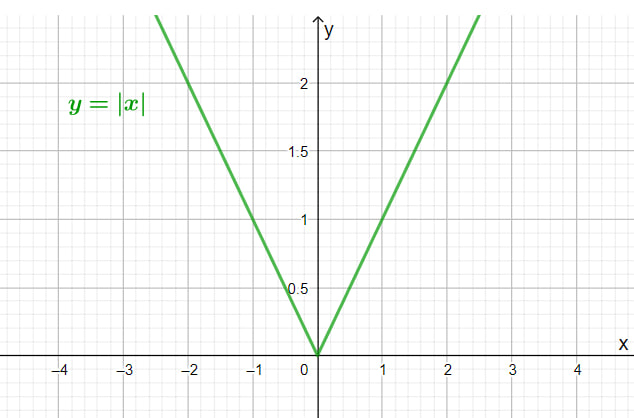
\includegraphics{images/abs(x).jpg}
    \caption{График функции $f(x) = |x|.$}
    \label{fig:enter-label}
\end{figure}
    
    Рассмотрим предел
    \begin{eqnarray*}
        \lim_{x \to 0}\frac{f(x) - f(0)}{x - 0} &=& \lim_{x \to 0} \frac{|x| - 0}{x-0} \\
        &=&\lim_{x \to 0} \frac{|x|}{x}\\
        &=& \lim_{x \to 0}\mathrm{sign}(x),
    \end{eqnarray*}
    где $\mathrm{sign}(x) : = \begin{cases}
        1, & x > 0, \\
        0, & x =0, \\
        -1 , & x <0,
    \end{cases}$
    но эта функция не непрерывна в точке $x_0$, а значит, и нет предела $\lim_{x \to 0}\frac{f(x) - f(0)}{x - 0}$, что и означает, что эта функция недифференцируема в точке $x_0 = 0.$

\end{example}

\begin{figure}[h!]
    \centering
    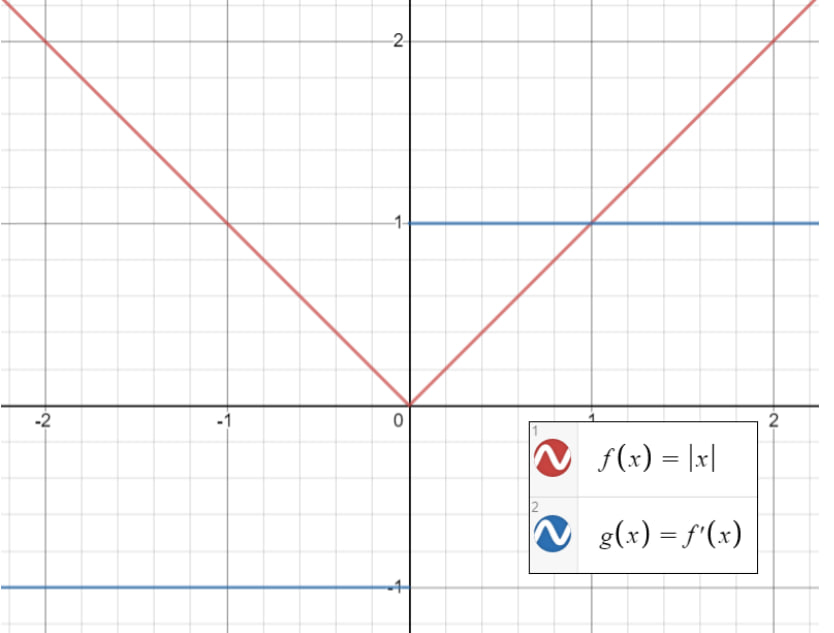
\includegraphics[scale = 0.7]{images/abs(x)+sign(x).jpg}
     \caption{Красным показан график функции $f(x) = |x|$, а синим -- график функции $g(x) = \mathrm{sign}(x)$, мы видим, что $g(x)$ делает резкий скачок в точке $0$, что и означает, что функция $f(x)$ недифференцируема.}
\end{figure}


\begin{example}
Одним из самых ярких контрпримеров является функция Вейерштрасса -- всюду непрерывная, но нигде не дифференцируемая функция. 
Аналитически она записывается следующим образом:

\[
f(x) = \sum_{n=0}^{\infty} {a^n \cos(b^n \pi x)},
\]
где $0 < a < 1, \; b$ -- положительное нечётное целое и
\[
ab > 1 + \frac{3 \pi}{2}
\]


\begin{figure}[h!]
    \centering
    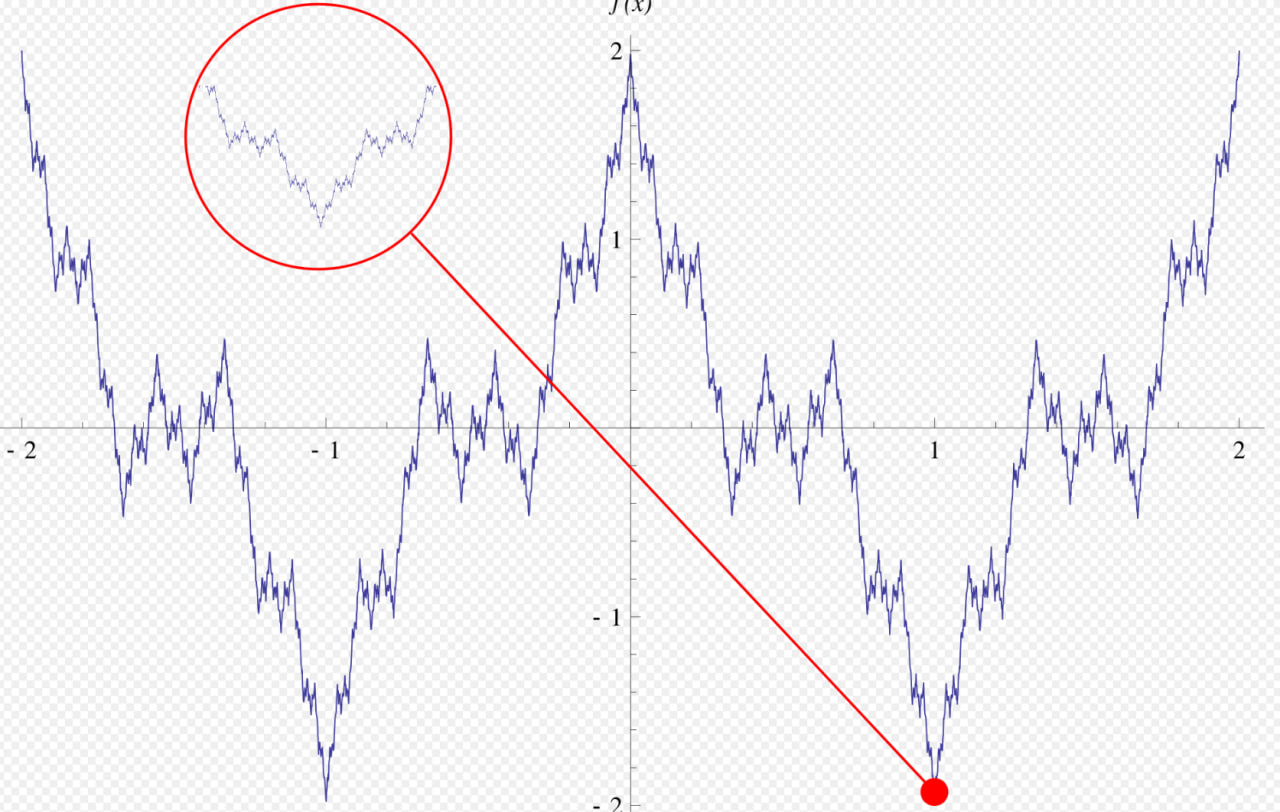
\includegraphics[width=1\linewidth]{images/WeierstrassFunction.jpeg}
    \caption{Простыми словами, функция Вейерштрасса резко меняет своё направление в каждой точке, поэтому не может быть дифференцируемой, но она также всюду непрерывна как предел равномерно сходящихся всюду непрерывных частичных сумм.    }
\end{figure}
\end{example}

\subsection{Свойства производной}

\begin{theorem}\label{ariph_for_der}
    Если функции $f(x), g(x)$ дифференцируемы в точке $x_0$, то:
    \begin{enumerate}
        \item $(f+g)'(x_0) = f'(x_0) + g'(x_0)$;
        \item $(fg)'(x_0) = f'(x_0) g(x_0) + f(x_0) g'(x_0);$
        \item $\left( \dfrac{f}{g} \right)'(x_0) = \dfrac{f'(x_0)g(x_0) - f(x_0) g'(x_0)}{(g(x_0))^2}$
    \end{enumerate}
\end{theorem}
\begin{proof}~

(1) Это сразу следует из того, что предел суммы -- это сумма пределов.

(2) Имеем
\begin{eqnarray*}
    (fg)'(x_0) &:=& \lim_{x \to \to x_0} \frac{f(x)g(x) - f(x_0)g(x_0)}{x-x_0} \\
    &=& \lim_{x \to x_0} \frac{ f(x)g(x)  - f(x_0) g(x) + f(x_0) g(x) - f(x_0)g(x_0)  }{x-x_0} \\
    &=& \lim_{x \to  x_0} \frac{ (f(x) - f(x_0))g(x)  + f(x_0) ( g(x) - g(x_0) )  }{x-x_0},
\end{eqnarray*}

По условию $f,g$ -- дифференцируемы в точке $x_0$, тогда согласно теореме \ref{diff_of_function_on_R}, $f,g$ -- непрерывны в точке $x_0$, а тогда согласно теореме \ref{criteria_of_continous} $\lim_{x\to x_0} f(x) = f(x_0)$ и $\lim_{x\to x_0}g(x) = g(x_0)$. 

Используя теперь арифметику предела (см. Теорему \ref{lim(f+g)}), получаем
\begin{eqnarray*}
    (fg)'(x_0) &=& \lim_{x \to  x_0} \frac{ (f(x) - f(x_0))g(x)  + f(x_0) ( g(x) - g(x_0) )  }{x-x_0} \\
    &=& \lim_{x \to x_0} \frac{f(x) - f(x_0)}{x-x_0} \cdot \lim_{x \to x_0} g(x) + f(x_0) \cdot \lim_{x \to x_0} \frac{g(x) - g(x_0)}{x-x_0} \\
    &=& f'(x_0)\cdot g(x_0) + f(x_0)\cdot g'(x_0).
\end{eqnarray*}

(3) Имеем
\begin{eqnarray*}
    \left( \dfrac{f}{g} \right)'(x_0) &=& \lim_{x\to x_0} \dfrac{ \dfrac{f(x)}{g(x)} - \dfrac{f(x_0)}{g(x_0)} }{x-x_0} \\
    &=& \lim_{x\to x_0} \left( \frac{f(x) g(x_0) - f(x_0) g(x)}{x-x_0}\cdot \frac{1}{g(x) g(x_0)} \right)\\
    &=& \lim_{x \to x_0}\left( \dfrac{f(x) g(x_0) - f(x_0)g(x_0) + f(x_0)g(x_0) - f(x_0)g(x)}{x-x_0} \cdot \frac{1}{g(x) g(x_0)} \right).
\end{eqnarray*}

Опять по условию $f,g$ -- дифференцируемы в точке $x_0$, тогда согласно теореме \ref{diff_of_function_on_R}, $f,g$ -- непрерывны в точке $x_0$, а тогда согласно теореме \ref{criteria_of_continous} $\lim_{x\to x_0} f(x) = f(x_0)$ и $\lim_{x\to x_0}g(x) = g(x_0)$. 

Используя теперь арифметику предела (см. Теорему \ref{lim(f+g)}), получаем
\begin{eqnarray*}
   \left( \dfrac{f}{g} \right)'(x_0) &=& \lim_{x \to x_0}\left( \dfrac{f(x) g(x_0) - f(x_0)g(x_0) + f(x_0)g(x_0) - f(x_0)g(x)}{x-x_0} \cdot \frac{1}{g(x) g(x_0)} \right) \\
   &=& \lim_{x \to x_0}\left( \dfrac{f(x) g(x_0) - f(x_0)g(x_0) + f(x_0)g(x_0) - f(x_0)g(x)}{x-x_0}\right) \cdot\left( \lim_{x\to x_0} \frac{1}{g(x) g(x_0)} \right) \\
   &=& \frac{1}{(g(x_0))^2}\cdot \cdot \left( \lim_{x \to x_0} \frac{f(x) - f(x_0)}{x-x_0}\cdot g(x_0)  - f(x_0) \cdot \lim_{x\to x_0} \frac{g(x) - g(x_0)}{x-x_0}  \right) \\
   &=& \frac{f'(x_0)g(x_0) - f(x_0)g'(x_0)}{(g(x_0))^2}.
\end{eqnarray*}



\end{proof}






\begin{theorem}\label{d(fg)}
Пусть $f: \mathscr{U} \to \mathbb{R}$ дифференцируема в $x_0 \in \mathscr{U}$, $g: \mathscr{W} \to \mathbb{R}$ дифференцируема в $y_0= f(x_0)$. Тогда $g \circ f :\mathscr{U} \to \mathbb{R}$ дифференцируемa в $x_0$ и 
    \[
   \mathrm{d} ( g\circ f)_{x_0} = (\mathrm{d}g)_{y_0} \cdot (\mathrm{d}f)_{x_0}.
    \]
\end{theorem}


\begin{proof}

 Так как $f$ дифференцируема, мы имеем
 \[
 f(x_0 + h) - f(x_0) = (\mathrm{d}f)_{x_0}(h) + \alpha(h) \cdot h,
 \] 
 и
 \[
  g(f(x_0) + v)) - g(f(x_0)) = (\mathrm{d}g)_{y_0}(v) + \beta(v)\cdot v
 \]
где $\lim_{h \to 0} \alpha (h) = 0$, $\lim_{v \to 0} \beta (v) = 0$.

Тогда, согласно определению предела (см. Определение \ref{the_main_def_of_limit_on_R}), мы можем положить $\alpha(0), \beta(0) := 0$.

Пусть $v: =f(x_0 + h) - f(x_0)$. Так как, согласно условию $f$ -- дифференцируема в точке $x_0$, тогда (см. Теорема \ref{diff_of_function_on_R}) она непрерывна в точке $x_0$, а тогда (см. Теорему \ref{criteria_of_continous}), если $h\to 0$, то $v \to 0$. 

Имеем

\begin{eqnarray*}
    g(f(x_0 +h)) -g(f(x_0)) &=& (\mathrm{d}g)_{y_0} \cdot \bigl(f(x_0+h) - f(x_0)\bigr)  \\
    &+& \beta\Bigl( f(x_0+h) - f(x_0) \Bigr) \cdot (f(x_0+h) - f(x_0)) \\
    &=& (\mathrm{d}g)_{y_0} \Bigl( (\mathrm{d}f)_{x_0}(h) + \alpha(h) \cdot h\Bigr) \\
    &+& \beta\Bigl(  (\mathrm{d}f)_{x_0}(h) + \alpha(h) \cdot h \Bigr) \cdot \Bigl(  (\mathrm{d}f)_{x_0}(h) + \alpha(h) \cdot h \Bigr)
\end{eqnarray*}
из-за линейности $(\mathrm{d}g)_{y_0}$ получаем
\begin{eqnarray*}
    g(f(x_0 +h )) -g(f(x_0)) &=&\Bigl((\mathrm{d}g)_{y_0 } \cdot (\mathrm{d}f)_{x_0}\Bigr) (h) + (\mathrm{d}g)_{ y_0} \cdot \alpha( h) \cdot h \\
    &+& \beta\Bigl( (\mathrm{d}f)_{x_0}\cdot h + \alpha(h) \cdot h \Bigr) \cdot \Bigl(  (\mathrm{d}f)_{x_0}\cdot h + \alpha(h) \cdot h \Bigr).     
\end{eqnarray*}

Запишем теперь это равенство так

\begin{eqnarray*}
    g(f(x_0 +h )) -g(f(x_0)) &=&\Bigl((\mathrm{d}g)_{y_0 } \cdot (\mathrm{d}f)_{x_0}\Bigr) (h) + (\mathrm{d}g)_{ y_0} \cdot \alpha( h) \cdot h \\
    &+& \beta\Bigl( \bigl( (\mathrm{d}f)_{x_0}+ \alpha(h) \bigr) \cdot h \Bigr) \cdot \Bigl(  (\mathrm{d}f)_{x_0} + \alpha(h) \Bigr)\cdot h.     
\end{eqnarray*}

Положим
\[
 \gamma(h): = (\mathrm{d}g)_{ y_0} \cdot \alpha( h)  + \beta\Bigl( \bigl( (\mathrm{d}f)_{x_0}+ \alpha(h) \bigr) \cdot h \Bigr) \cdot \Bigl(  (\mathrm{d}f)_{x_0} + \alpha(h) \Bigr),
\]
тогда
\[
  g(f(x_0 +h )) -g(f(x_0)) = \Bigl((\mathrm{d}g)_{y_0 } \cdot (\mathrm{d}f)_{x_0}\Bigr) (h) + \gamma(h)\cdot h.
\]

В силу непрерывности $\alpha(h), \beta(h)$ в точке $h=0$ и существования в точке $x_0$ дифференциалов $(\mathrm{d}f)_{x_0}:=f'(x_0)$, $(\mathrm{d}g)_{y_0}:=g'(y_0)$, мы, используя теорему о композиции (см. Теорема \ref{comp_of_continous_on_R}), тогда получаем
\begin{eqnarray*}
 \lim_{h \to 0} \gamma(h) &=& \lim_{h\to 0} \Bigl( (\mathrm{d}g)_{ y_0} \cdot \alpha( h)  + \beta\Bigl( \bigl( (\mathrm{d}f)_{x_0}+ \alpha(h) \bigr) \cdot h \Bigr) \cdot \Bigl(  (\mathrm{d}f)_{x_0} + \alpha(h) \Bigr) \Bigr) \\
 &=& (\mathrm{d}g)_{ y_0} \cdot \lim_{h\to 0} \alpha( h)  + \beta\Bigl( \bigl( (\mathrm{d}f)_{x_0}+  \lim_{h\to 0}\alpha(h) \bigr) \cdot \lim_{h\to 0} h \Bigr) \cdot \Bigl(  (\mathrm{d}f)_{x_0} + \lim_{h\to 0}\alpha(h) \Bigr) \\
 &=& 0 + \beta(0)\cdot (f'(x_0))\\
 &=& 0.
\end{eqnarray*}

Тогда мы показали, что
\[
 g(f(x_0 +h )) -g(f(x_0)) =\Bigl((\mathrm{d}g)_{y_0 } \cdot (\mathrm{d}f)_{x_0}\Bigr) (h) + o(h), \qquad h \to 0 
\]
или
\[
 g(f(x_0 +h ))  = g(f(x_0))+\Bigl((\mathrm{d}g)_{y_0 } \cdot (\mathrm{d}f)_{x_0}\Bigr) (h) + o(h), \qquad h \to 0
\]
откуда
\[
\mathrm{d}(g\circ f)_{x_0} = (\mathrm{d}g)_{y_0 } \cdot (\mathrm{d}f)_{x_0},
\]
что и доказывает утверждение.
\end{proof}



\subsection{Геометрический смысл дифференциала функции}



\begin{theorem}
    Пусть функция $f(x)$ дифференцируема в точке $x_1$, а прямая $\ell$, проходящая через точки $(x_1,y_1)$, $(x_2,y_2)$, где $y_1 = f(x_1)$, $y_2 = f(x_2)$, задаётся уравнением $y = k(x_2) (x - x_1 ) + y_1$. Тогда
    \[
     \lim_{x_2 \to x_1} k(x_2) = f'(x_1).
    \]
\end{theorem}
  
\begin{figure}[h!]
    \centering
    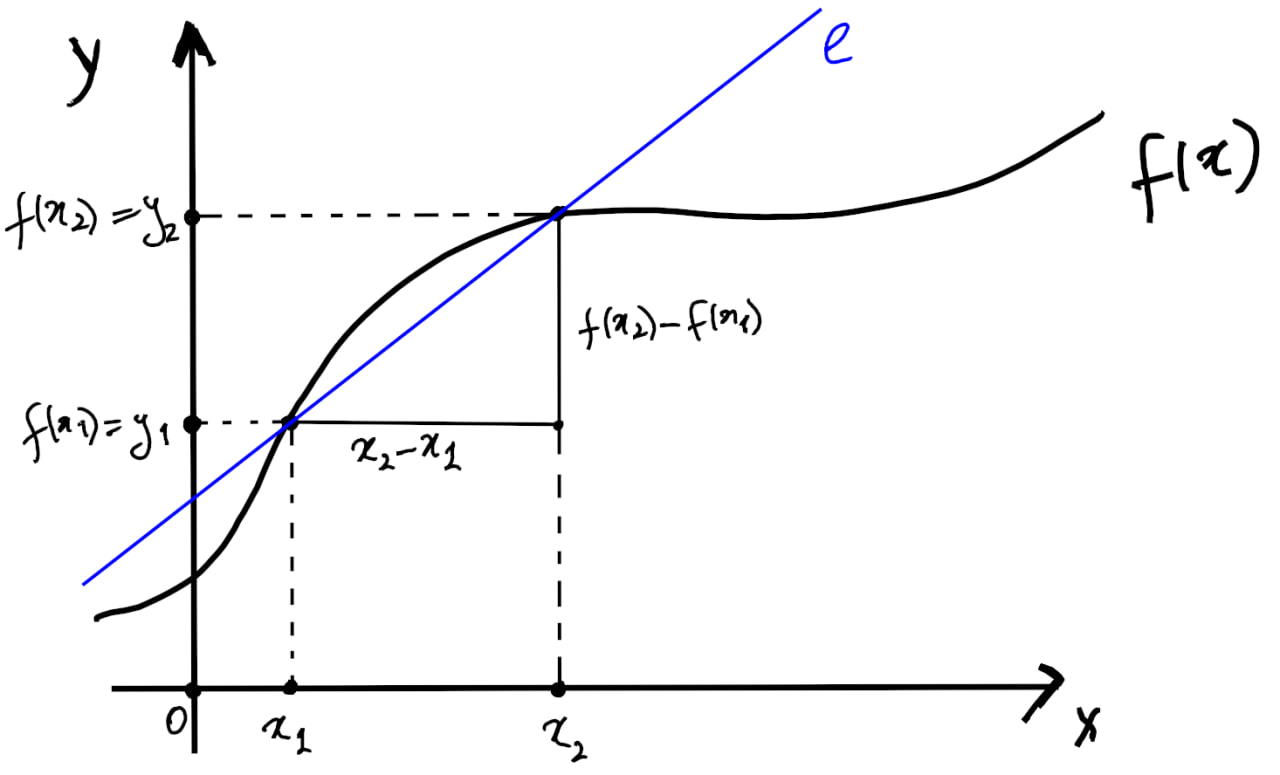
\includegraphics[scale = 0.4]{images/line_and_f'.jpg}
    \caption{Прямая $\ell$, проходящая через точки $(x_1,y_1)$, $(x_2,y_2)$, где $y_1 = f(x_1)$, $y_2 = f(x_2)$}
    \label{fig:enter-label}
\end{figure}

\begin{proof}
    Рассматриваемая прямая задаётся уравнением 
\[
 y = \frac{f(x_2) - f(x_1)}{x_2 - x_1}(x-x_1) +y_1,
\]
поэтому
\[
 k(x_2)  = \frac{f(x_2) - f(x_1)}{x_2 - x_1}.
\]

Тогда из определения производной следует, что
\[
 \lim_{x_2 \to x_1}k(x_2) = f'(x_1).
\]
\end{proof}

\begin{definition}
    Прямую $y = f'(x_0)(x-x_0) + f(x_0)$ называют \textit{касательной} к графику $y = f(x)$ в точке $(x_0, f(x_0)).$
\end{definition}

\begin{figure}[h!]
    \centering
    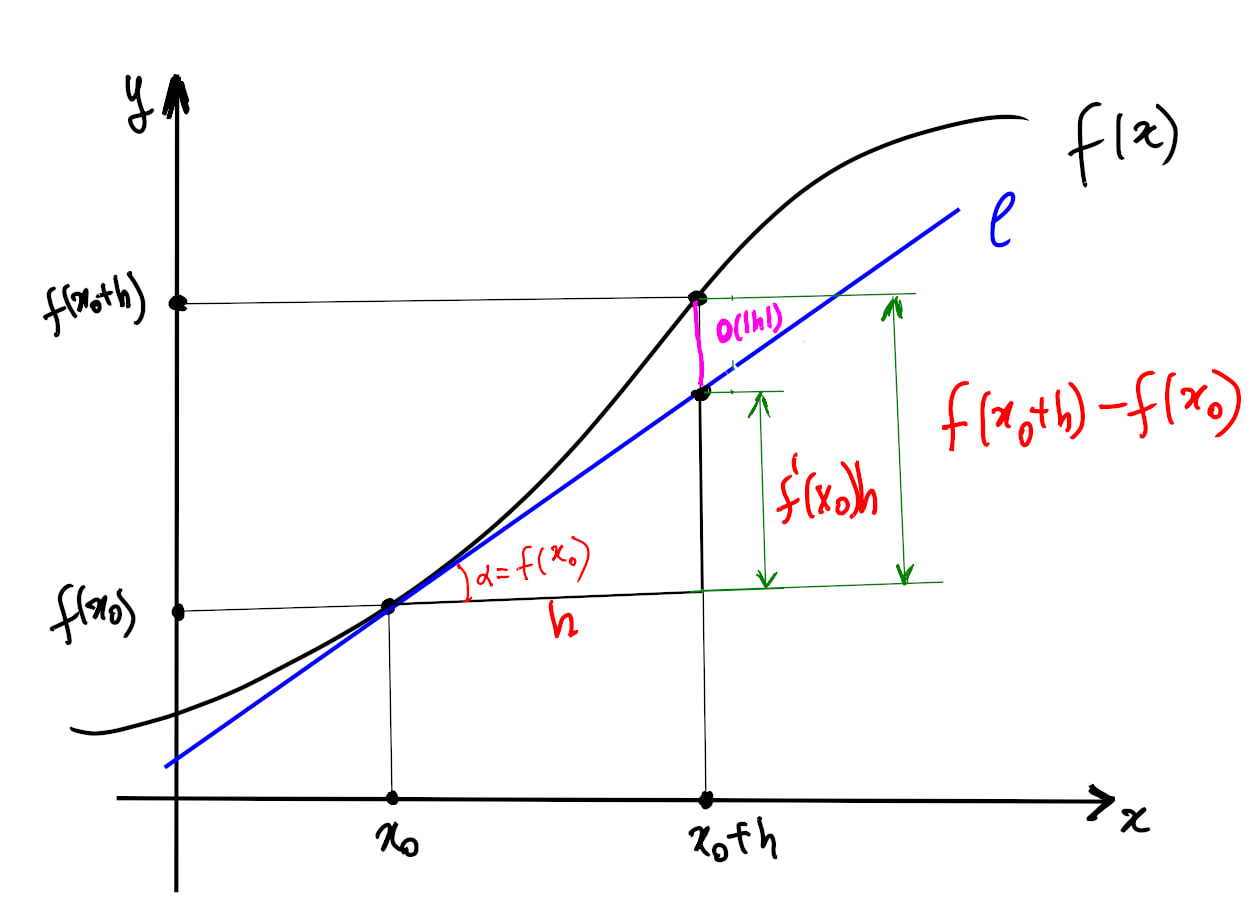
\includegraphics[scale= 0.4]{images/tan_and_f.jpg}
    \caption{Таким образом, если функция $f(x)$ дифференцируема в точке $x_0$, то её можно приблизить линейной функцией $f'(x_0)(x-x_0) +f(x_0)$, при этом $o(h)$ показывает, насколько далеко это приближение.}
    \label{fig:enter-label}
\end{figure}





\section{Лекция \#17. Функции на компактном множестве}

Как мы знаем (см. Теорема \ref{criterai_of_compacness_in_R}), любое компактное множество на $\mathbb{R}$ содержится в отрезке, то все наши рассуждения будут вестись над отрезком конечной длины.

\subsection{Непрерывность на компактном множестве}

\begin{theorem}[о промежуточном значении]\label{intermediat_theorem}
 Если функция $f(x)$ непрерывна на отрезке $[a,b]$ и принимает на его концах значения разных знаков, то $f(x_0) = 0$ для некоторой точки $x_0 \in [a,b]$.    
\end{theorem}
\begin{proof}
    Пусть $f(a)>0$, $f(b)<0$.  Построим последовательности $(a_n)$, $(b_n)$ следующим образом; $a_1:=a$, $b_1:=b$,
\begin{align*}
    &a_{n+1}:= \begin{cases}
        \frac{a_n +b_n}{2}, & \mbox{если $f(\frac{a_n +b_n}{2})>0$},\\
        a_n, & \mbox{если $f(\frac{a_n +b_n}{2})<0$},
    \end{cases}  & b_{n+1}:= \begin{cases}
        \frac{a_n +b_n}{2}, & \mbox{если $f(\frac{a_n +b_n}{2})<0$},\\
        b_n, & \mbox{если $f(\frac{a_n +b_n}{2})>0$},
        \end{cases}
\end{align*}
при $n\ge 1$.

Покажем, что $a_{n+1}\le b_{n+1}$. По условию $a_1: = a < b =:b_1$. Пусть $a_n \le b_n$. Рассмотрим тогда $a_{n+1}$, $b_{n+1}$. Тогда, если $a_{n+1} = \frac{a_{n}+b_n}{2}$. то $b_{n+1} = b_n$, и тогда 
\[
 a_{n+1} = \frac{a_n+b_n}{2} < \frac{b_n + b_n}{2} = b_n = b_{n+1}.
\]
Если же $a_{n+1} = a_n$, то $b_{n+1} = \frac{a_n + b_n}{2}$, и мы получаем
\[
 b_{n+1} = \frac{a_n + b_n}{2} > \frac{a_n + a_n}{2} = a_n = a_{n+1}.
\]

Итак, мы показали, что $a_n \le b_n$. Далее покажем, что $a_{n+1} \ge a_n$. Действительно, либо $a_2= a_1$, либо $a_2 = \frac{a_1 + b_1}{2} = \frac{a+b}{2} > \frac{a+a}{2} = a = a_1$. Пусть $a_{n} \ge a_{n-1}$, тогда если $a_{n+1} = \frac{a_n + b_n}{2}$, то $b_{n+1} = b_n$, то
\[
 a_{n+1} = \frac{a_n + b_n}{2} \ge \frac{a_n + a_n}{2} = a_n,
\]
иначе $a_{n+1} = a_n$.

Аналогично показывается, что $b_{n+1} \le b_{n}$.

В итоге, мы получили две ограниченные\footnote{потому что они находятся в отрезке!} монотонные последовательности $(a_n)$, $(b_n)$. Тогда по теореме Вейерштрасса \ref{Weierstrass} у них есть предел.

С другой стороны, имеем
\[
 b_{n+1} - a_{n+1} = \begin{cases}
      \frac{a_n+b_n}{2} - a_n = \frac{b_n - a_n}{2}, & \mbox{если $b_{n+1} = \frac{a_n + b_n}{2}$ и тогда $a_{n+1} = a_n$}, \\
      b_n - \frac{a_n + b_n}{2} = \frac{b_n - a_n}{2}, & \mbox{если $b_{n+1} = b_n$ и тогда $a_{n+1} = \frac{a_n + b_n}{2}$}
 \end{cases}, 
\]
\ie
\[
 b_{n+1} - a_{n+1} = \frac{b_n - a_n}{2} =  \frac{b - a}{2^{n}}.
\]
\end{proof}

Тогда получаем
\[
 \lim_{n \to \infty} (b_n - a_n) = \lim_{n \to \infty} \frac{b-a}{2^{n-1}} =0,
\]
\ie $\lim_{n \to \infty} a_n = \lim_{n \to \infty} b_n =x_0.$

Так как функция непрерывна, и $x_0$ есть точка прикосновения отрезка $[a,b]$, то по теореме  \ref{lim=>for_any_sequence}, $f(x_0) = \lim_{n \to \infty} f(a_n) = \lim_{n \to \infty} f(b_n)$. С другой стороны, по построению последовательности все $f(a_n) \ge 0$, $f(b_n)\le 0$, тогда по теореме \ref{lim(f+g)},
\[
 \lim_{n \to \infty} f(a_n)\ge 0, \qquad  \lim_{n \to \infty} f(b_n)\le 0,
\]
 но тогда $f(x_0) =  \lim_{n \to \infty} f(a_n) =  \lim_{n \to \infty} f(b_n) = 0$, что и требовалось. 


\begin{mydangerr}{\bf!}
 Эту теорему формулируют также следующим образом.
\end{mydangerr}

\begin{corollary}\label{mean_value_theorem}
    Пусть функция $f:[a,b] \to \mathbb{R}$ -- непрерывная функция, пусть $f(a) \ne f(b)$, и без ограничения общности предположим, что $f(a) < f(b)$, тогда для любого $\xi\in [f(a), f(b)]$ существует такой $x_0 \in [a,b]$, что $f(x_0) = \xi.$
\end{corollary}

\begin{proof}
    Действительно, для лююбого фиксированного числа $f(a) \le \xi \le f(b)$, функция $g_\xi(x) := f(x) - \xi$ является непрерывной на $[a,b]$ ибо она есть сумма непрерывных функций. Далее, $g(a) = f(a) - \xi <0$ и $g(b) = f(b) - \xi >0$, тогда согласно предыдущей теореме, найдётся такой $x_0 \in [a,b]$, что $f(x_0) = \xi$, что и требовалось доказать.
\end{proof}

\begin{definition}
    Значение функции, которое является наибольшим или наименьшим, называется \textit{экстремальным}. Точку, в которой функция принимает экстремальное значение, называют \textit{точкой экстремума}. Если же рассматривается какая-то окрестность точки $x_0$ и оказывается, что $x_0$ точка экстремума, то говорят, что $x_0$ есть точка \textit{локального экстремума.} 
\end{definition}


\begin{theorem}\label{continous_on_interval_on_R}
    Функция $f(x)$, непрерывная на отрезке $[a,b]$, ограничена на этом отрезке.
\end{theorem}
\begin{proof}
    Докажем, что она ограничена сверху (ограниченность снизу доказывается аналогично). Пусть для любого $n\in \mathbb{N}$ на отрезке $[a,b]$ есть такая точка $x_n$, что $f(x_n) >n$. Мы получаем ограниченную последовательность $(x_n)$, тогда по теореме \ref{from_bounded_sequence} можно выбрать сходящуюся подпоследовательность $(x_{n_k})$. Пусть тогда $\lim_{n\to \infty}x_{n_k} = x_0$. Согласно лемме \ref{a<b}, $a\le x_0 \le b$. 

    Далее, так как $f(x)$ непрерывна на всём отрезке, то $f(x_0) = \lim_{x\to x_0}f(x)$, но тогда, согласно теореме \ref{lim=>for_any_sequence}, $f(x_0)  = \lim_{n\to \infty} f(x_{n_k})$, но мы предположили, что $f(x_{n_k}) > n_k$, тогда $\lim_{n\to \infty} f(x_{n_k}) = \infty$, что даёт противоречие.
\end{proof}

\begin{theorem}(Вейерштрасс)\label{W2_on_R}
    Функция $f(x)$, непрерывная на отрезке $[a,b]$, достигает максимума и минимума в некоторых точках этого отрезка.
\end{theorem}
\begin{proof}

Рассмотрим множество $\Bigl\{f(x),\, x \in [a,b] \Bigr\}$. Очевидно, что оно не пусто. Согласно теореме \ref{continous_on_interval_on_R}, оно ограничено. Тогда, согласно принципу полноты Вейерштрасса (теорема \ref{W=complete}), это множество имеет $\sup$ и $\inf$.

Покажем\footnote{для $\inf$ доказательство аналогичное}, что на отрезке $[a,b]$ есть такая точка $x_0$, для которой $f(x_0) = M$, где
\[
M: = \sup_{a \le x \le b}\{f(x)\}.
\]

Итак, множество $\Bigl\{f(x),\, x\in  [a,b] \Bigr\}$ ограничено и не пусто и имеет $\sup, \inf$. Тогда из определения \ref{sup,inf} следует, что найдутся такие $f(x_n)$, что 
$$M - \frac{1}{n} \le f(x_n) \le M$$
для какой-то последовательности $(x_n)$ точек из $[a,b]$. Согласно теореме \ref{from_bounded_sequence}, можно выбрать сходящуюся подпоследовательность $(x_{n_k})$. Пусть пределом этой подпоследовательности будет $x_0$. Тогда согласно теореме \ref{a<b}, $a\le x_0 \le b$, так $(x_n) \subseteq [a,b].$

Тогда согласно теореме \ref{lim=>for_any_sequence}, $f(x_0)  = \lim_{n \to \infty} f(x_{n_k})$, но так как $M - \frac{1}{n} \le f(x_n) \le M$, то по лемме о зажатой последовательности (теорема \ref{sqeezy}), $f(x_0) = M$, что и требовалось доказать. 
\end{proof}

\begin{theorem}\label{image_of_compact}
    Пусть $f:K\to \mathbb{R}$ -- непрерывная функция, $K \subseteq \mathbb{R}$, тогда если $K$ -- компактно, то $f(K)$ -- компактно.
\end{theorem}

\begin{proof}
    Пусть $\{\mathscr{U}'_\alpha\}_{\alpha \in A}$ -- покрытие $f(K)$ открытыми в $\mathbb{R}$ множествами, тогда семейство $\{f^{-1}(\mathscr{U}'_\alpha)\}_{\alpha \in A}$ -- покрытие $K$, и так как $f$ -- непрерывно, то по Теореме \ref{preimage_of_open}, это покрытие открытыми множествами в $K.$ Так как $K$ -- компактно, то можно найти конечное подпокрытие, скажем, $\{f^{-1}(\mathscr{U}'_i)\}_{i=1}^n$, но тогда $\{\mathscr{U}_i\}_{i=1}^n$ -- покрытие для $f(K)$, что и показывает компактность $f(K).$
\end{proof}



\subsection{Теоремы о среднем}


\begin{theorem}[Ферма]\label{Ferma}
    Пусть функция $f(x)$ определена на отрезке $[a,b]$, $(a,b) \ni x_0$ -- точка экстремума, и $f'(x_0)$ существует. Тогда $f'(x_0) = 0$.
\end{theorem}

\begin{proof}
    Пусть $f(x_0) \le f(x)$ для всех $x \in [a,b]$, другой случай рассматривается аналогично. Рассмотрим пределы
    \[
    A:= \lim_{x \in \mathbb{R}_{>x_0}, x\to x_0} \frac{f(x) - f(x_0)}{x-x_0}, \qquad B:=\lim_{x \in \mathbb{R}_{x<x_0}, x\to x_0} \frac{f(x) - f(x_0)}{x-x_0}.
    \]

Так как $f'(x_0) := \lim_{x\in \mathbb{R}, x \to x_0}$ существует, значит, по Теореме \ref{limit_for_any_subset} эти два предела должны совпадать. Но так как  $f(x_0) \le f(x)$, то по теореме \ref{lim(f+g)}, $A\ge 0$, $B\le 0$, но тогда $f'(x_0) =0$, что и требовалось. 
\end{proof}


\begin{theorem}(Ролль) \label{Roll}
    Пусть функция $f(x)$ дифференцируема на отрезке $[a,b]$, причём $f(a) = f(b)$. Тогда существует такая точка $x_0 \in (a,b)$, что $f'(x_0) = 0.$
\end{theorem}

\begin{proof}
    Согласно теореме Вейештрасса \ref{W2_on_R}, $f(x)$ достигает максимума $M$ и минимума $m$ на этом отрезке.

    (1) Пусть $M = m$, тогда $f(x) = \mathrm{const}$, так как $m \le f(x) \le M$ для всех $x \in [a,b]$. Тогда в качестве $x_0$ можно взять любую точку из $(a,b)$.

    (2) Пусть $f(x) \ne \mathrm{const}$, тогда найдётся точка $x_0 \in (a,b)$ такая, что $f(x_0) \ne f(a) =f(b)$. Положим $f(x) > f(a)$. Далее, согласно теореме Вейерштрасса \ref{W2_on_R}, найдётся точка $x_1 \in [a,b]$, в которой $f(x_1)$ максимальна. Тогда $x_1 \ne a,b$ и по теореме Ферма (теорема \ref{Ferma}) мы получаем требуемое. 
\end{proof}


С геометрической точки зрения теорема утверждает, что если ординаты обоих концов гладкой кривой равны, то на кривой найдется точка, в которой касательная к кривой параллельна оси абсцисс.

Механический смысл теоремы в том, что если некоторое тело вернулось в исходную точку, двигаясь по незамкнутой линии, то оно обязано было хотя бы раз остановиться до нулевой скорости.

\begin{theorem}[Лагранж]\label{Langrange}
    Пусть функция $f(x)$ дифференцируема на отрезке $[a,b]$. Тогда существует такая точка $x_0 \in (a,b)$, что 
    \[
     f'(x_0) = \frac{f(b) - f(a)}{b-a}
    \]
\end{theorem}

\begin{proof}
    Рассмотрим функцию
    \[
     \varphi(x)  = f(x) - \frac{f(b) - f(a)}{b-a}(x-a).
    \]
Эта функция дифференцируема на отрезке $[a,b]$ и $\varphi(a) = \varphi(b) =  f(a)$, тогда по теореме Ролля (теорема \ref{Roll}) существует $x_0 \in (a,b)$ такая, что $\varphi'(x_0) = 0$, \ie
\[
 \varphi'(x_0) = f'(x_0) - \frac{f(b) - f(a)}{b-a} = 0,
\]
что и требовалось доказать.
\end{proof}

\begin{mydanger}{\bf{!}}
    Эту теорему часто записывают в виде $f(b) - f(a)=  f'(x_0)(b-a)$ и называют \textit{формулой конечных приращений} или \textit{теоремой о среднем значении}.
\end{mydanger}

\begin{mydanger}{\bf{!!}}
    Иногда бывает удобно рассмотреть функцию $f$ на отрезке $[a, a+h]$. Тогда теорема Лагранжа утверждает, что существует такое $\theta \in (0,1)$, что $f(a+h) - f(a) = f'(a+\theta h)\cdot h.$
\end{mydanger}

\begin{corollary}[Критерий монотонности]\label{monoton_criteria}
    Дифференцируемая функция $f:[a,b] \to \mathbb{R}$ не убывает тогда и только тогда, когда $f'(x) \ge 0$ для любого $x \in [a,b].$
\end{corollary}
\begin{proof}~

(1) Пусть $f$ -- не убывает, то для любого $h \ge 0$, $f(x_0 + h ) \ge f(x_0)$. Далее, так как по условию предел
\[
 f'(x_0) : = \lim_{h \to 0} \frac{f(x_0 + h) - f(x_0)}{h} 
\]
существует, то согласно Теореме \ref{limit_for_any_subset},
\[
 f'(x_0) = \lim_{h \to 0+} \frac{f(x_0 + h) - f(x_0)}{h}
\]
и тогда $f'(x_0) \ge 0$.

(2) Пусть теперь $f'(x)\ge 0$ для любого $x \in [a,b]$ и пусть $y\in [a,b]$, $x <y$. Тогда по теореме Лагранжа (см. Теорема \ref{Langrange}), существует такая точка $\theta \in (x,y)$, что 
\[
 f(y) - f(x) = f'(\theta) (y-x),
\]
так как $f'(\theta) \ge 0$, то $f(y) \ge f(x)$, то и доказывает не убывание функции.    
\end{proof}



\begin{theorem}[Коши]\label{Coushy_for_functions}
    Пусть функции $f(x)$, $g(x)$ дифференцируемы на отрезке $[a,b]$, причём $g'(x) \ne 0$ на $(a,b)$. Тогда существует такая $c \in (a,b)$, что 
    \[
     \frac{f(b) -f(a)}{g(b) - g(a)} = \frac{f'(c)}{g'(c)}.
    \]
\end{theorem}

\begin{proof}
    Пусть
    \[
     F(x): = \bigl(f(b)-f(a) \bigr) (g(x)-g(a)) - ( f(x)- f(a)) \bigl(g(b) - g(a)\bigr).
    \]

    Ясно, что
    \[
     F'(x) = \bigl(f(b)-f(a) \bigr) g'(x) - f'(x)\bigl(g(b) - g(a)\bigr)
    \]
и $F(a) = F(b) =0$. Тогда по теореме Ролля \ref{Roll} существует $c\in (a,b)$ такая, что $F'(c) = 0.$

Если $g(b) = g(a)$, то по теореме Ролля нашлась бы точка $x_0 \in (a,b)$ такая, что $g'(x_0) = 0$, но по условию $g' \ne 0$ на всём $(a,b)$, тогда $g(b) \ne g(a)$. Поэтому из $F'(c)=0$ и следует требуемое.

\end{proof}


\section{Лекция \#18. Правило Лопиталя}


\begin{theorem}[Лопиталь]\label{Lop}
    Пусть $f,g$ -- дифференцируемы на $(a,b)$ и $g' \ne 0$ на $(a,b)$ и выполнено одно из двух условий
    \begin{enumerate}
        \item $\lim\limits_{x \to x_0-} f(x) = \lim\limits_{x \to x_0 -}g(x) = 0$, 
        \item $\lim\limits_{x \to x_0-}g(x) = \infty.$
    \end{enumerate}

Тогда если $\lim\limits_{x \to x_0-} \dfrac{f'(x)}{g'(x)} = A$, то $\lim\limits_{x \to x_0-} \dfrac{f(x)}{g(x)} = A.$
\end{theorem}

\begin{mydanger}{\bf !}
    Требование про то чтобы $\lim_{x\to x_0-}f(x) = \infty$ во втором условии вообще говоря излишне.
\end{mydanger}

\begin{proof}
(1) Пусть $f(x_0) = g(x_0) = 0$, тогда наши функции $f,g$ непрерывны в $x_0$. Тогда по теореме Коши \ref{Coushy_for_functions},
\begin{equation}\label{for_Lop}
 \frac{f(x)}{g(x)} = \frac{f(x) - f(x_0)}{g(x) - g(x_0)} = \frac{f'(y)}{g'(y)},    
\end{equation}
где $y \in (x, x_0)$. Так как $\lim_{x \to x_0} \frac{f'(x)}{g'(x)} = A$, то для любого $\varepsilon >0$, можно найти такое $\delta>0$, что для любого $x_0-\delta < z < x_0$, получаем
\[
\left| \frac{f'(z)}{g'(z)} -A\right| < \varepsilon.
\]

Пусть теперь $x \in (x_0 - \delta, \delta)$, то воспользовавшись (\ref{for_Lop}),
\[
 \left| \frac{f(x)}{g(x)} - A \right| = \left| \frac{f'(z)}{g'(z)} -A \right| < \varepsilon,
\]
что и доказывает требуемое.

(2) Так как функции дифференцируемы на $(a,b)$ и $g' \ne 0$ на $(a,b)$, то по теореме Коши \ref{Coushy_for_functions}, 
\[
\frac{f(b) -f(a)}{g(b) - g(a)} = \frac{f'(c)}{g'(c)},
\]
перепишем его в виде
\[
 (f(b) - f(a)) g'(c) = f'(c) (g(b) - g(a)),
\]
поделим на $g(b)$, получаем
\[
 \left(\frac{f(b)}{g(b)} - \frac{f(a)}{g(b)} \right) g'(c) = f'(c) \left(1 - \frac{g(a)}{g(b)} \right)
\]
теперь поделим всё на $g'(c)$
\[
 \frac{f(b)}{g(b)} - \frac{f(a)}{g(b)}  = \frac{f'(c)}{g'(c)}\left(1 - \frac{g(a)}{g(b)} \right)
\]
получаем
\[
 \frac{f(b)}{g(b)}  = \frac{f'(c)}{g'(c)}\left(1 - \frac{g(a)}{g(b)} \right) + \frac{f(a)}{g(b)}.
\]

Имеем $(x_0 - \theta, x_0 + \theta) \cap \mathbb{R}_{< x_0} = (x_0 -\theta, x_0).$ Поэтому получаем, что если $\lim\limits_{x \to x_0-} \dfrac{f'(x)}{g'(x)} = A$, то для любого $\varepsilon>0$ найдётся такой $y$, что для любого $z \in (y, x_0)$ имеем 
\[
 \left| \frac{f'(z)}{g'(z)} - A \right| < \varepsilon.
\]

С другой стороны, это неравенство также означает что в какой-то окрестности $x_0$ функция $\frac{f'(z)}{g'(z)}$ ограничена, \textit{т.е.,} можно записать $\left| \dfrac{f'(z)}{g'(z)} \right|<C$, например, можно положить, что $C:=|A|+1.$

Фиксируем $y$, так как $\lim_{x \to x_0-}g(x) = \infty$, то $\lim_{x \to x_0-}\frac{1}{g(x)} = 0$, то для уже выбранного выше $\varepsilon>0$ можно найти такое $\delta>0$, что для любого $x \in (x_0 - \delta, x_0)$, получаем
\[
 \left| \frac{g(y)}{g(x)} \right| < \varepsilon, \qquad \left| \frac{f(y)}{g(x)}  \right| < \varepsilon.
\]

Имеем
\begin{eqnarray*}
    \left| \frac{f(x)}{g(x)} -A\right| &=& \left| \frac{f'(c)}{g'(c)}- A - \frac{f'(c)}{g'(c)} \cdot \frac{g(y)}{g(x)}  + \frac{f(y)}{g(x)}\right| \\
    &\le & \left|\frac{f'(c)}{g'(c)}- A \right| + \left| \frac{f'(c)}{g'(c)} \cdot \frac{g(y)}{g(x)}\right| + \left|  \frac{f(y)}{g(x)}\right| \\
    &<& \varepsilon + C\cdot \varepsilon + \varepsilon \\
    &=& (C+2)\varepsilon,
\end{eqnarray*}
что и доказывает требуемое.
\end{proof}

\section{Лекция \#19. Высшие производные}

\subsection{Основные определения}

Рассмотрим дифференцируемую функцию $f:\mathscr{U} \to \mathbb{R}$ на каком-то открытом множестве $\mathscr{U} \subseteq \mathbb{R}$, \textit{т.е.,} для каждой точки $p\in \mathscr{U}$ мы имеем функцию
\[
 f': \mathscr{U} \to \mathbb{R}, \qquad \mathscr{U} \ni p \mapsto f'(p).
\]


\begin{definition}
Если функция $f':\mathscr{U} \to \mathbb{R}$ -- дифференцируема в точке $x_0$, то значение её производной в этой точке называют \textit{второй производной} и при этом пишут    
\[
 f''(x_0):=(f')'(x_0),
\]
дифференциал функции $f'$ называют \textit{вторым дифференциалом} и пишут
\[
 \mathrm{d}^2f:= \mathrm{d}(\mathrm{d}f').
\]
\end{definition}

По индукции мы теперь можем ввести понятие третьей производной, четвёртой \textit{и.т.д.,} и тоже касается дифференциалов. 

\begin{mydanger}{\bf !}
    Третью производную принято обозначать так $f'''$, а вот далее, уже пишут так $f^{(4)}$, $f^{(5)}$, \textit{и.т.д.}
\end{mydanger}

\begin{example}
    Рассмотрим функцию 
    \[
     f(x) = \begin{cases}
         \dfrac{1}{2}x^2, & x \ge 0\\
         -\dfrac{1}{2}x^2, & x \le 0
         \end{cases}
    \]

\begin{figure}[h!]
    \centering
    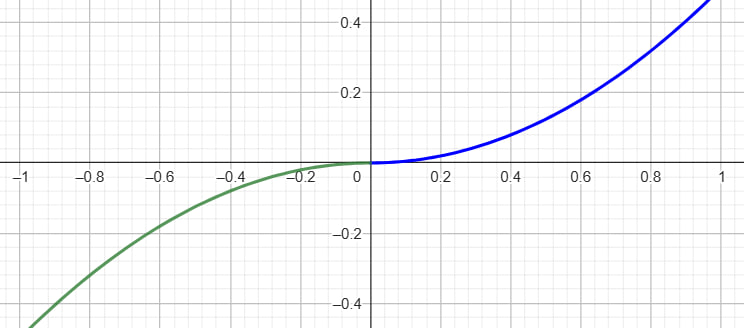
\includegraphics[width=0.7\linewidth]{images/x^2.jpg}
    \caption{График функции $f(x)$, эта функции непрерывна и дифференцируема в точке $x_0=0$, но вторая производная в этой точке у этой функции не существует.}
    \label{fig:enter-label}
\end{figure}

Имеем
\[
 f'(x) = \begin{cases}
     x, & x \ge 0,\\
     -x, & x \le 0
 \end{cases} = |x|,
\]
а как мы уже знаем, (см. Пример \ref{|x|is_not_diff}, эта функция уже не дифференцируема в точке $x=0.$

\begin{figure}
    \centering
    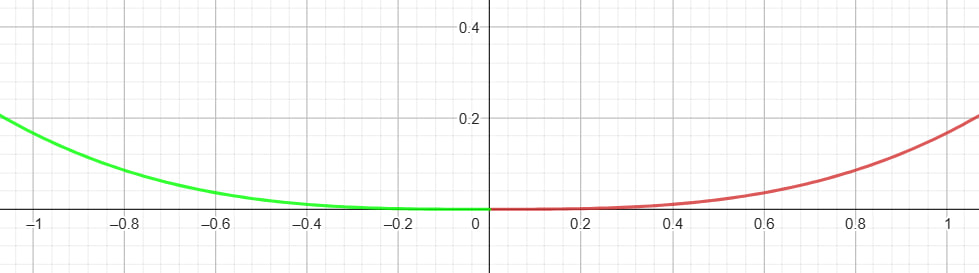
\includegraphics[width=0.7\linewidth]{images/x^3.jpg}
    \caption{Функция $g(x)$ дважды, но трижды дифференцируема в точке $x_0=0$.}
    \label{fig:enter-label}
\end{figure}

Аналогично можно показать, что функция
\[
 g(x) = \begin{cases}
     \dfrac{1}{6} x^3, & x \ge 0,\\
     -\dfrac{1}{6} x^3, & x \le 0,
 \end{cases}
\]
дважды, но не трижды дифференцируема в точке $x_0=0$.
\end{example}


\begin{remark}
    С другой стороны, ясно, что если функция имеет $n$-ую производную, то значит, она имеет $n-1$-ую производную, а значит и $n-2$-ую \textit{и.т.д.}
\end{remark}

Множество всех $n$-раз дифференцируемых функций на множестве $X \subseteq \mathbb{R}$ принято обозначать так $C^n(X)$, при этом, полагают, что $C^0(X)$ -- множество всех непрерывных функций на $C$.

Согласно Теореме \ref{ariph_for_der}, эти множества есть векторные пространства над $\mathbb{R}$, при этом $C^{m}(X)$ -- подпространство в $C^n(X)$, при $m \ge n$. Таким образом, имеем цепочку подпространств 
\[
 C^0(X) \supseteq C^1(X) \supseteq C^2(X) \supseteq \ldots,
\]

\begin{definition}
Если функция дифференцируема сколь угодно много раз на множестве $X\subseteq \mathbb{R}$, то такую функцию называют \textit{гладкой на $X$.} Пространство гладких функций на $X$ обозначают так $C^\infty(X).$ 
\end{definition}

Примерами гладких функций на $\mathbb{R}$ являются любые полиномы, а также функции $\sin(x)$, $\cos(x)$, $\mathrm{exp}(x)$.



\subsection{Полином Тейлора от одной переменной}

Рассмотрим полином $P(x) \in \mathbb{R}[x]$. Говорят, что полином $P(x)$ \textit{разложен в точке $a$ по степеням $(x-a)$}, если существуют такие $c_0, c_1, \ldots, c_n$, где $n = \mathrm{deg}(P(x))$, что $P(x) = c_0 + c_1(x-a) + c_2(x-a)^2 + \cdots + c_n(x-a)^n$. 

Нетрудно видеть, что эти коэффициенты можно найти следующим образом
\[
 c_0 = P(a), \quad c_1 = P'(a), \quad c_2 = \frac{1}{2}P''(a), \quad c_3 = \frac{1}{6}P'''(a), \ldots,  c_n = \frac{1}{n!}P^{(n)}(a).
\]

Таким образом, получаем
\[
 P(x) = P(a) + P'(a)(x-a) + \frac{1}{2} P''(a)(x-a)^2 + \cdots + \frac{1}{n!}P^{(n)}(a)(x-a)^n.
\]


\begin{definition}
    Пусть $f(x)$ есть $n$-раз дифференцируема в точке $a\in \mathbb{R}$. Полином вида 
    \[
     T_f(x): = \sum_{k=0}^n \frac{f^{(k)}(a)}{k!}(x-a)^k
    \]
    называется \textit{полиномом Тейлора для функции $f$}.
\end{definition}


\begin{theorem}
    Если $f$ есть $n$-раз дифференцируемая функция в точке $a$, то
    \[
     f(x) = T_f(x) + o((x-a)^n), \qquad x \to a.
    \]
\end{theorem}

\begin{proof}
    Пусть $r(x): = f(x) - T_f(x)$, очевидно, что $r(a) = r'(a) = \cdots = r^{(n)}(a) = 0$. По правилу Лопиталя \ref{Lop}
    \begin{eqnarray*}
        \lim_{x \to a} \frac{r(x)}{(x-a)^n} &=& \lim_{x \to a} \frac{r'(x)}{n(x-a)^{n-1}} \\
        &=& \lim_{x \to a} \frac{r''(x)}{n(n-1)(x-a)^{n-2}} = \cdots \\
        &=& \lim_{x \to a} \frac{r^{(n-1)}(x)}{n!(x-a)}
    \end{eqnarray*}
Дальше правило Лопиталя применять вообще говорят нельзя, так как по условию известно, что существует лишь $f^{(n)}(a)$, а в окрестности она может не существовать. 

Воспользуемся теперь определением, получаем
\[
 r^{(n)}(a) = \lim_{x \to a} \frac{r^{(n-1)}(x) - r^{(n-1)}(a)}{(x-a)} = \lim_{x \to a} \frac{r^{(n-1)}(x)}{(x-a)},
\]
потому что $r^{(n-1)}(a) = 0$, но тогда
\[
 \lim_{x \to a} \frac{r^{(n-1)}(x)}{n!(x-a)} = \frac{1}{n!}\lim_{x \to a} \frac{r^{(n-1)}(x)}{x-a} = \frac{1}{n!} r^{(n)}(a)= 0,
\]
что и доказывает требуемое.
\end{proof}

\begin{theorem}[Общий вид остаточного монома]\label{gen_monom}
    Пусть $f$ есть $n$ раз дифференцируема в каждой точке отрезка $[a,x]$, функция $f^{(n)}$ непрерывна на $[a,x]$ и дифференцируема на интервале $(a,x)$. Пусть $g(x)$ непрерывна на $[a,x]$ и дифференцируема на $(a,x)$, причём $g\ne 0$ на $(a,x)$. Тогда существует такое $c\in (a,x)$, что
    \[
     f(x) = \sum_{k=0}^n \frac{f^{(k)}(a)}{k!}(x-a)^k + r_n(x,a),
    \]
    где 
    \[
     r_n(x,a) = \frac{1}{n!}\frac{f^{(n+1)}(c)}{g'(c)}\bigl(g(x) - g(a)\bigr)(x-c)^n.
    \]
\end{theorem}
\begin{proof}
Пусть
\begin{eqnarray*}
  \psi(t) &:=& f(x) - \sum_{k=0}^n \frac{f^{(k)}(t)}{k!}(x-t)^k \\
  &=& f(x) - \left(f(t) + f'(t)(x-t) + \cdots + \frac{1}{n!}f^{(n)}(t)(x-t)^n \right) 
\end{eqnarray*}
где $a \le t \le x$.

Тогда
\[
 \psi(x) = 0, \qquad \psi(a) = f(x) - \sum_{k=0}^n \frac{f^{(k)}(a)}{k!}(x-a)^k,
\]
\textit{т.е.,} $r_n(x,a) = \psi(a)$.

Согласно условиям, $\psi(t)$ дифференцируема на $[a,x]$, тогда по теореме Коши \ref{Coushy_for_functions}, существует такое $c \in (a,x)$, что
\[
 \frac{\psi(x)-\psi(a)}{g(x) - g(a)} = \frac{\psi'(c)}{g'(c)},
\]
тогда
\[
 \psi(a) = - \frac{\psi'(c)}{g'(c)}(g(x) - g(c))
\]
поэтому
\[
 r_n(x,a)= - \frac{\psi'(c)}{g'(c)}(g(x) - g(c)).
\]

Имеем
\begin{eqnarray*}
    \psi'(t) &= & - \left( f(t) + f'(t)(x-t) + \frac{1}{2!}f''(t)(x-t)^2 + \frac{1}{3!}f'''(t)(x-t)^3 + \cdots \frac{1}{n!}f^{(n)}(t) (x-t)^n \right)' \\
    &=& -f'(t) \\
    && - f''(t)(x-t) + f'(t) \\
    && - \frac{1}{2!}f'''(t)(x-t)^2 + f''(t)(x-t) \\
    &&  - \frac{1}{3}f^{(4)}(x-t)^3 + \frac{1}{3!}f'''(t)(x-t)^3 \\
    && \cdots - \frac{f^{(n+1)}(t)}{n!}(x-t)^n \\
    &=& - \frac{f^{(n+1)}(t)}{n!}(x-t)^n.
\end{eqnarray*}

Таким образом,
\[
 r_n(x,a) =\frac{1}{n!}\frac{f^{(n+1)}(c)}{g'(c)}\bigl(g(x) - g(a)\bigr)(x-c)^n,
\]
что и требовалось доказать.    
\end{proof}


\begin{corollary}[Остаточный моном в форме Коши]
    \[
     \begin{boxed}{
         r_n(x,a) = \frac{f^{(n+1)}(c)}{n!}(x-a)(x-c)^n, \quad a < c <x.}
     \end{boxed}
    \]
\end{corollary}
\begin{proof}
    Нужно положить $g(x) = x-t$ в теореме \ref{gen_monom}.
\end{proof}

\begin{corollary}[Остаточный моном в форме Лагранжа.]\label{monom_in_Langrange}
    \[
     \boxed{
      r_n(x,a) = \frac{f^{(n+1)}(c)}{(n+1)!}(x-a)^{n+1}, \qquad a < c <x.
     }
    \]
\end{corollary}
\begin{proof}
    Нужно положить $g(x) = (x-t)^{n+1}.$
\end{proof}


\subsection{Выпуклость и вогнутость}

\begin{definition}
 Функция $f:[a,b] \to \mathbb{R}$, называется \textit{выпуклой на отрезке} $[a,b]$, если для любых $x_1,x_2 \in [a,b]$ выполняется неравенство
 \[
  f \left( \frac{x_1+x_2}{2} \right) \le \frac{f(x_1) + f(x_2)}{2}.
 \]

 Функция $f(x)$ называется \textit{вогнутой на отрезке} $[a,b]$, если функция $-f(x)$ ---выпукла на $[a,b].$
\end{definition}

\begin{lemma}\label{convex_for_n}
 Если $f:[a,b] \to \mathbb{R}$ -- выпукла, то для любых $x_1,\ldots, x_n \in [a,b]$,
 \[
  f \left( \frac{x_1+ \cdots + x_n}{n} \right) \le \frac{f(x_1) + \cdots + f(x_n)}{n}.
 \]
\end{lemma}
\begin{proof}
 Это сразу следует из определения выпуклости и применения метода индукции. 
\end{proof}

\begin{proposition}\label{convex_proposition}
    Пусть $f:[a,b] \to \mathbb{R}$ -- выпукла на $[a,b]$, $p,q \ge 0$, $p+q=1$.
    \begin{enumerate}
        \item Если $p,q\in \mathbb{Q}$, то $f(px_1 + qx_2) \le p f(x_1) + q f(x_2)$.
        \item Если $f$ -- непрерывна на $[a,b]$, то 
        \[
         f(px_1 + qx_2) \le p f(x_1) + q f(x_2),
        \]
 для любых $p,q \ge 0$, с условием $p+q=1$.
    \end{enumerate}
\end{proposition}

\begin{proof}~

(1)  Пусть $p,q \in \mathbb{Q}$, тогда, в виду условия $p+q=1$, имеются такие $m \in \mathbb{Z}_+$, $n \in \mathbb{N}$, что $p = \frac{m}{n}$, $q = \frac{n-m}{n}$.

По лемме \ref{convex_for_n}, получаем
\begin{eqnarray*}
 f(px_1 + qx_2) &=& f\left( \frac{m}{n}x_1 + \frac{n-m}{n} x_2 \right) = f\left( \frac{mx_1 + (n-m)x_2}{n} \right) \\
 &=&   f\Bigl( \frac{\overbrace{x_1 + \cdots +x_1}^m + \overbrace{x_2 + \cdots +x_2}^{n-m}}{n}\Bigr)  \\
 &\le& \frac{mf(x_1) + (n-m)f(x_2)}{n} \\
 &=& \frac{m}{n} f(x_1) + \frac{n-m}{n} f(x_2) \\
 &=& pf(x_1) + q f(x_2),
\end{eqnarray*}
что и требовалось доказать.

(2) Пусть теперь $f$ -- непрерывна на отрезке $[a,b]$, и пусть $p,q \in \mathbb{R}$, $p,q \ge 0$, $p+q =1$. Так как $\overline{\mathbb{Q}} = \mathbb{R}$ (см. отдел \ref{barQ=R}), то можно найти такие последовательности $(p_n)$, $(q_n)$ положительных рациональных чисел $p_n, q_n \in \mathbb{Q}$, что $\lim_{n\to \infty} p_n = p$, $\lim_{n\to \infty}q_n =q$.\footnote{Можно и проще, так как моделью $\mathbb
R$ являются бесконечные десятичные дроби, то если, скажем, 
$$p = \alpha_0. \alpha_1\alpha_2\alpha_3\cdots$$
бесконечная дробь, то последовательность рациональных чисел 
\[
 \alpha_0, \quad \alpha_0.\alpha_1, \quad  \alpha_0.\alpha_1\alpha_2, \quad \alpha_0.\alpha_1\alpha_2\alpha_3, \quad \ldots
\]
сходится к $p.$
} Более того, согласно теореме \ref{a+b,ca,ab}, $p_n + q_n = 1$ для всех $n \in \mathbb{N}.$

Тогда, согласно Теореме \ref{a+b,ca,ab}, $\lim_{n\to \infty} (p_n x_1 + q_n x_2 ) = pz_1 + q x_2$, и теперь, используя Теорему \ref{lim=>for_any_sequence} (=определение по Гейне), получаем
\begin{equation}\label{convex_theorem_1}
  \lim_{n\to \infty} f(p_n x_1 + q_n x_2) = f(px_1 + qx_2).    
\end{equation}

С другой стороны, согласно теореме \ref{a+b,ca,ab}, получаем
\begin{equation}\label{convex_theorem_2}
  \lim_{n\to \infty} \left( p_n f(x_1) + b_n f(x_2)\right) = p f(x_1) + q f(x_2).    
\end{equation}


Далее, так как $f$ -- выпукла на $[a,b]$, то, согласно доказанному пункту (1), для рациональных чисел $p_n,q_n$, для которых верно $p_n, q_n \ge 0$, $p_n + q_n =1$, имеем
\[
 f(p_nx_1 + q_n x_2) \le p_n f(x_1) + q_n f(x_2),
\]
тогда согласно теореме \ref{lim(f+g)},
\[
\lim_{n\to \infty} f(p_nx_1 + q_n x_2) \le \lim_{n\to \infty} \left( p_n f(x_1) + q_n f(x_2) \right),
\]
учитывая теперь (\ref{convex_theorem_1}), (\ref{convex_theorem_2}), получаем
\[
 f(px_1 + q x_2) \le p f(x_1) + q f(x_2).
\]

Это завершает доказательство.
\end{proof}

\begin{corollary}\label{cor_for_convex}
    Если $f:[a,b] \to \mathbb{R}$ -- непрерывная и выпукла, то для любого $x \in (a,b)$,
    \[
     \frac{f(x) - f(a)}{x-a} \le \frac{f(b) - f(x)}{b-x}.
    \]
\end{corollary}
\begin{proof}
Пусть $p:= \frac{b-x}{b-a}$ и $q: = \frac{x-a}{b-a}$. Видно, что $p,q \ge 0$, и $p+q=1$, тогда согласно предложению \ref{convex_proposition}, для любых $p,q \ge 0$, $p+q=1$, $f(px_1 + qx_2) \le pf(x_1) + qf(x_2)$.

Так как $x = \frac{b-x}{b-a} \cdot a + \frac{x-a}{b-a}\cdot b$, то получаем
\[
 f(x) = f\left(  \frac{b-x}{b-a} \cdot a + \frac{x-a}{b-a}\cdot b\right) \le \frac{b-x}{b-a} f(a) + \frac{x-a}{b-a}f(b).
\]

Таким образом, получаем

\[
 (b-a)f(x) \le (b-x) f(a) + (x-a) f(b).
\]

Далее, так как $b-a = (b-x) - (a-x)$, то можно записать
\[
 (b-a) f(x) = \left( (b-x) - (a-x) \right) f(x) = (b-x)f(x) - (a-x)f(x),
\]
тогда используя неравенство выше, получаем
\[
 (b-x)f(x) - (a-x)f(x) \le (b-x) f(a) + (x-a) f(b),
\]
а это можно переписать так
\[
 (b-x) (f(x) - f(a)) \le (x-a) (f(b) - f(x)),
\]
или что равносильно неравенству 
 \[
     \frac{f(x) - f(a)}{x-a} \le \frac{f(b) - f(x)}{b-x},
    \]
что и требовалось доказать.
\end{proof}

\begin{theorem}
    Пусть $f: [a,b] \to \mathbb{R}$ -- дифференцируемая функция на отрезке $[a,b]$. Тогда $f$ -- выпукла тогда и только тогда, когда $f'$ не убывает на $[a,b]$.
\end{theorem}
\begin{proof}~

(1) Пусть $f$ -- выпукла,  и пусть $a \le x_1 < x < x_2 \le b$, тогда согласно следствию \ref{cor_for_convex}, 
\[
 \frac{f(x) - f(x_1)}{x-x_1} \le \frac{f(x_2) -  f(x)}{x_2- x}.
\]

Тогда, согласно теореме \ref{lim(f+g)} (=предел от неравенств) и определению производной (см. Определение \ref{derivative_of_function}), имеем
\[
 \lim_{x \to x_1} \frac{f(x) - f(x_1)}{x-x_1} =:f'(x_1) \le \lim_{x \to x_1} \frac{f(x_2) -  f(x)}{x_2- x} = \frac{f(x_2) -  f(x_1)}{x_2- x_1}
\]
а также 
\[
 \lim_{x \to x_2}  \frac{f(x) - f(x_1)}{x-x_1} =  \frac{f(x_2) - f(x_1)}{x_2-x_1} \le \lim_{x\to x_2} \frac{f(x_2) -  f(x)}{x_2- x} =: f'(x_2).
\]

Итак, мы получили, что 
\[
 f'(x_1) \le \frac{f(x_2) -  f(x_1)}{x_2- x_1} \le f'(x_2), 
\]
\textit{т.е.,} имеем $f'(x_1) \le f'(x_2)$ для любых $a \le x_1  < x_2 \le b$, а это и доказывает не убывание функции $f'.$

(2) Пусть теперь функция $f'$ не убывает на $[a,b]$, тогда согласно теореме Лагранжа (см. Теорема \ref{Langrange}), для любых $a \le x_1 < x < x_2 \le b$ существуют такие $\theta_1 \in (x_1, x)$, $\theta_2 \in (x,x_2)$, что
\[
 f'(\theta_1) = \frac{f(x) - f(x_1)}{x-x_1}, \qquad f'(\theta_2) = \frac{f(x_2) - f(x)}{x_2-x}.
\]

Так как мы предположили, что $f'$ не убывает на отрезке $[a,b]$ и так как $\theta_1 < \theta_2$, то $f'(\theta_1) \le f'(\theta_2)$, но тогда
\[
 \frac{f(x) - f(x_1)}{x-x_1} \le \frac{f(x_2) - f(x)}{x_2-x},
\]
но согласно следствию \ref{cor_for_convex} это и означает выпуклость функции $f$ на отрезке $[a,b].$ Это завершает доказательство.
\end{proof}

\begin{corollary}
    Если функция $f:[a,b] \to \mathbb{R}$ дважды дифференцируема на $[a,b]$, то $f$ выпукла на $[a,b]$ тогда и только тогда, когда $f''(x) \ge 0$ для любого $x \in [a,b].$
\end{corollary}
\begin{proof}
    Это сразу следует из предыдущей теоремы и критерием возрастания (см. Следствие \ref{monoton_criteria}).
\end{proof}

\begin{definition}
    Точка $x_0 \in [a,b]$ в которой $f''(x_0) =0$ называют \textit{точкой перегиба.}
\end{definition}

%\chapter{Интегрирование линейных дифференциальных форм}

В этой главе мы познакомимся с понятием интеграла. Мы будем развивать теорию интегрирования для функций от одной переменной. Прежде всего, мы напомним важные факты из дифференциального исчисления функции от одной переменной.

\section{Линейные дифференциальные формы}

Нам понадобится напоминание понятия дифференциала и некоторое важное для дальнейшего соглашение.

Пусть имеется функция $f:\mathbb{R} \to \mathbb{R}$, мы говорим, что она дифференцируема в точке $x_0$, если существует такое линейное отображение $(\mathrm{d}f)_{x_0}: \mathbb{R} \to \mathbb{R}$, что имеет место равенство
\[
 f(x_0 + h) = f(x_0) + (\mathrm{d}f)_{x_0}(h) + o(|h|), \qquad h \to 0.
\]

\begin{figure}[h!]
    \centering
    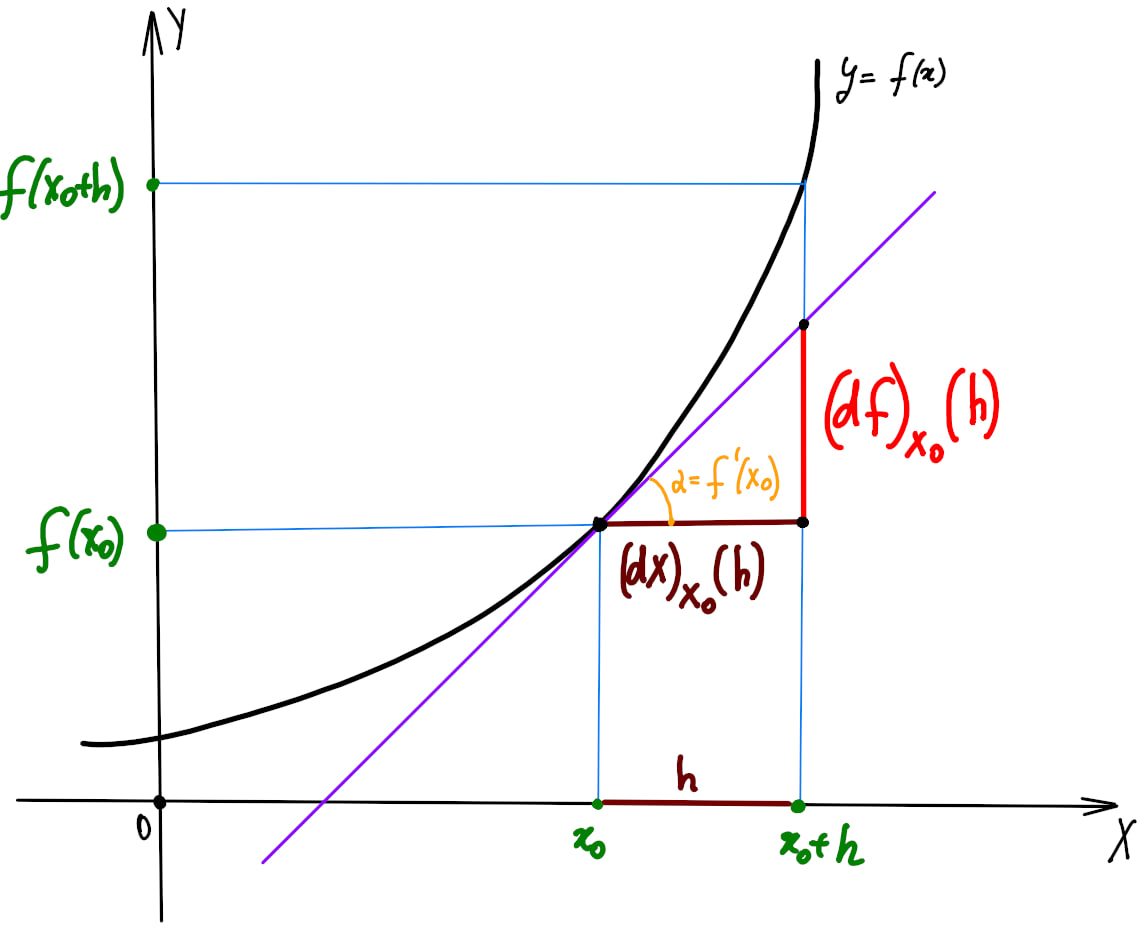
\includegraphics[scale=0.5]{images/df=f'dx.jpg}
    \caption{Caption}
    \label{fig:enter-label}
\end{figure}

При этом, как мы уже знаем, это линейное отображение $(\mathrm{d}f)_{x_0}$ называется дифференциалом функции $f$, вычисленным в точке $x_0$. Более того, имеем равенство
\[
 (\mathrm{d}f)_{x_0}(h): = f'(x_0)\cdot h, 
\]
где мы от $h \in \mathbb{R}$ уже, вообще говоря, ничего не требуем, но если $h\to 0$, то и $(\mathrm{d}f)_{x_0}(h) \to 0.$

Рассмотрим теперь функцию $y(x) = x$, тогда 
\[
 (\mathrm{d}x)_{x_0}(h) = (x'(x_0))\cdot h
\]
и так как $x' = 1$, мы получаем $(\mathrm{d}x)_{x_0}(h) = h$, тогда мы можем записать
\[
 (\mathrm{d}f)_{x_0}(h) = f'(x_0) \cdot h = f'(x_0) \cdot  (\mathrm{d}x)_{x_0}(h).
\]

Тогда мы можем сократить эту формулу следующим образом
\begin{equation}\label{df=f'dx}
  \boxed{
  \mathrm{d}f = f'\cdot \mathrm{d}x.
 }    
\end{equation}


\begin{mydanger}{\bf{!}}
    Нужно понимать, что полученная формула это \textbf{всего лишь соглашение!!!} Ведь эта формула должна пониматься как это написано выше, \textit{т.е.} $(\mathrm{d}f)_{x_0}(h) = f'(x_0) \cdot  (\mathrm{d}x)_{x_0}(h).$    
\end{mydanger}

\begin{remark}
Рассмотрим теперь $\mathbb{R}^n$ cо стандартным базисом $\mathbb{e} = (\m{e}_1,\ldots, \m{e}_n)$, тогда любой вектор $\m{h} = (h_1,\ldots, h_n)^\top  \in \mathbb{R}^n$ записывается в виде $\m{h} = h_1\m{e}_1 + \cdots + h_n \m{e}_n.$ 

Рассмотрим координатные функции 
\[
 x_1,\ldots, x_n:\mathbb{R}^n \to \mathbb{R}, \qquad x_i(\m{h}): = h_i, \quad 1 \le i \le n.
\]

Тогда их дифференциалы $(\mathrm{d}x_1, \ldots, \mathrm{d}x_n)$ -- это в точности базис двойственного пространства $(\mathbb{R}^n)^*$, так как
\[
 (\mathrm{d}x_i)(\m{e}_j) = \delta_{i,j}: = \begin{cases}
     1, & i = j, \\
     0, & i \ne j.
 \end{cases}
\]

Тогда, если $f:\mathbb{R}^n \to \mathbb{R}$ -- дифференцируемая функция в точке $\m{a}$, то её дифференциал (=градиент) можно записать так:
\begin{equation}\label{differential_via_dx}
  \boxed{
 \nabla_\m{a} f = \left.\frac{\partial f}{\partial x_1}\right|_\m{a} \cdot \mathrm{d}x_1 + \cdots +  \left.\frac{\partial f}{\partial x_n}\right|_\m{a} \cdot \mathrm{d}x_n.
    }    
\end{equation}

Действительно, имеем
\begin{eqnarray*}
    (\nabla_\m{a} f) (\m{h}) &=& \left.\frac{\partial f}{\partial x_1}\right|_\m{a} \cdot \mathrm{d}x_1(\m{h}) + \cdots +  \left.\frac{\partial f}{\partial x_n}\right|_\m{a} \cdot \mathrm{d}x_n (\m{h}) \\
    &=& \left.\frac{\partial f}{\partial x_1}\right|_\m{a} \cdot h_1 + \cdots +  \left.\frac{\partial f}{\partial x_n}\right|_\m{a} \cdot h_n ,
   \end{eqnarray*}
   что и есть определение дифференциала фукнции.
\end{remark}

\begin{mydanger}{\bf{!}}
    Это как раз и показывает, что градиент функции есть элемент двойственного пространства, \textit{т.е.} градиент -- это ковектор (=функционал), а не вектор!
\end{mydanger}

\begin{definition}
    Выражение вида 
    \[
     f_1 \mathrm{d}x_1 + \cdots + f_n \mathrm{d}x_n,
    \]
    где $f_1,\ldots, f_n:\mathbb{R}^n \to \mathbb{R}$ -- функции, называется \textit{линейной дифференциальной формой} или \textit{$1$-формой}, и обычно они обозначаются через $\omega$, а пространство всех линейных дифференциальных форм на $\mathbb{R}^n$ обозначается как $\Omega^1(\mathbb{R}^n).$
\end{definition}

\begin{example}
    Дифференциал функции всюду дифференцируемой функции как раз и есть пример дифференциальной формы. Например, пусть $f(x_1,x_2) = x_1^3 - 2x_1x_2 + 3x_2^2$, ясно, что это всюду дифференцируемая функция на $\mathbb{R}^2$. Находим
 \begin{eqnarray*}
   \frac{\partial f}{\partial x_1} &=& 3x_1^2 - 2x_2, \\
   \frac{\partial f}{\partial x_2} &=&  - 2x_1 + 6x_2,
 \end{eqnarray*}

Поэтому, учитывая (\ref{differential_via_dx}), получаем
\[
 \nabla f = (3x_1^2-2x_2)\mathrm{d}x_1 + (-2x_1 + 6x_2) \mathrm{d}x_2.
\]
    
\end{example}




\section{Понятие неопределённого интеграла}

Предыдущий пример доставляет нам множество линейных дифферециальных форм. Возникает естественный вопрос:~

\textit{Пусть нам дана произвольная линейная дифференциальная форма $\omega \in \Omega^1(\mathbb{R}^n)$, существует ли функция $f:\mathbb{R}^n \to \mathbb{R}$ такая, что $\nabla f = \omega$?}

\textbf{Ответом на этот вопрос и занимается теория интегрирования.}

Мы же ограничимся случаем, когда $f$ есть функция от одной переменной, \textit{т.е.} мы будем развивать теорию интегрирования для $\Omega^1(\mathbb{R}).$

Для дальнейшего нам понадобится следующее: 
\begin{definition}
    Промежутком в $\mathbb{R}$ мы называем любое множество, являющееся либо отрезком, либо интервалом, либо полуоткрытым интервалом.
\end{definition}

Понятие неопределённого интеграла возникает при решении следующей задачи:
\textit{пусть мы знаем некоторую функцию $f(x)$, существует ли такая функция $F(x)$, что $F'(x) =f(x)?$}

\begin{definition}\label{int1}
    Функция $F(x)$ в данном промежутке называется \textit{интегралом} (=\textit{первообразной}) для функции $f(x)$, если во всём этом промежутке $f(x)$ является производной для функции $F(x)$ или, что тоже, $f(x)\mathrm{d}x$ есть линейная дифференциальная форма, равная дифференциалу функции $F(x)$
    \[
     F'(x) = f(x) \quad \mbox{или} \quad  \mathrm{d}F = f(x) \mathrm{d}x.
    \]
\end{definition}

\begin{theorem}\label{int1=int2+C}
    Если в некотором промежутке $I \subseteq \mathbb{R}$ функция $F(x)$ есть интеграл для функции $f(x)$, то и функция $F(x) + C$, где $C$ -- любая постоянная (=число), также будет интегралом для $f(x)$. Более того, любые два интеграла $F(x)$, $G(x)$ для одной и той же функции $f(x)$ отличаются на некоторое число $C$, \textit{т.е.} $G(x) =F(x) + C.$
\end{theorem}

\begin{proof}~

(1) Если $F(x)$ -- интеграл для фукнции $f(x)$, то $F'(x) = f(x)$, а тогда
\[
 (F(x) + C)' = F'(x) + (C)' = f(x) + 0 = f(x),
\]
что и означает, что $F(x) +C$ тоже интеграл для $f(x).$

(2) Пусть $F(x), G(x)$ -- два интеграла для фукнции $f(x)$ на промежутке $I$. Пусть $\Phi(x): = F(x) - G(x)$, тогда для любого $x_0 \in I$ имеем $\Phi'(x_0) = 0$. Возьмём (Аксиома Выбора позволяет) другую точку $x \in I$, тогда в зависимости от знака $x_0 - x$ либо $[x_0, x] \subseteq I$, либо $[x,x_0] \in I$. В любом случае, мы имеем выполнение требований теоремы Лагранжа (см. Теорему \ref{Langrange}) для функции $\Phi(x)$. Таким образом, найдётся точка $c \in (x_0, x)$ (\textit{соотв.}, $c \in (x, x_0)$) такая, что
\[
 \Phi(x) - \Phi(x_0) = \Phi'(c)(x-x_0), 
\]
ясно, что $c \in I$, но тогда $\Phi'(c) = 0$, и мы получаем $\Phi(x) = \Phi(x_0) = C$ для любых двух $x,x_0 \in I$. Это завершает доказательство.    
\end{proof}

В силу этого мы вводим следующее определение, которое является очень важным для дальнейшего.

\begin{definition}\label{int2}
    Выражение $F(x) + C$, где $C$ -- произвольная постоянная, представляет собой \textbf{общий вид} функции, которая имеет производную $f(x)$, или её дифференциал есть $1$-форма $f(x) \mathrm{d}x.$

    Это выражение называется \textit{неопределённым интегралом} функции $f(x)$ и обозначается символом
    \[
     \int f(x) \mathrm{d}x,
    \]
    $f(x)$ называется \textit{подынтегральной функцией.}
\end{definition}

\begin{example}
    Пусть $f(x) = x^2$, тогда, как нетрудно догадаться,
    \[
     \int x^2 \mathrm{d}x = \frac{x^3}{3} + C.
     \]
Это легко проверить -- просто дифференцируя правое выражение, мы получим $x^2.$
\end{example}

    
\begin{mydanger}{\bf{!}}
    Ещё раз подчеркнём, что под знаком интеграла $\int$ пишут \textbf{дифференциальную $1$-форму}, а не производную! В предыдущем примере мы писали $\int x^2 \mathrm{d}x$, а не $\int x^2$! Такой способ записи, как будет позже показано, создался исторически; к тому же он представляет целый ряд преимуществ, и его сохранение вполне целесообразно. 
\end{mydanger}

\textbf{Таким образом, интегрируют не функцию $f(x)$, а  дифференциальную 
форму $f(x)\mathrm{d}x$!}

Покажем, что операции $\mathrm{d}$, $\int$ обратны друг к другу.

\begin{lemma}
    \[
     \mathrm{d} \int f(x)\mathrm{d}x = f(x) \mathrm{d}x, \qquad \left( \int f(x) \mathrm{d}x \right)' = f(x).
    \]
\end{lemma}

\begin{proof}
    Пусть $\int f(x) \mathrm{d}x = F(x)+C$, тогда, согласно определению \ref{int1}, $F'(x) = f(x)$, и тогда
    \[
    \left(\int f(x) \mathrm{d}x \right)' =  (F(x) + C)' = F'(x)  = f(x), 
    \]
откуда, согласно (\ref{differential_via_dx}),
\[
 \mathrm{d} \int f(x)\mathrm{d}x = f(x) \mathrm{d}x.
\]
\end{proof}

\begin{lemma}\label{intdF=F}
    Пусть $F(x)$ есть интеграл функции $f(x)$, тогда
    \[
     \int F'(x) \mathrm{d}x = F(x) +C, \qquad \int \mathrm{d}F(x) = F(x) + C.
    \]
\end{lemma}
\begin{proof}
    Если $F(x)$ -- интеграл функции $f(x)$, то согласно определению \ref{int1}, $F'(x) = f(x)$, и тогда
    \[
      \int F'(x) \mathrm{d}x = \int f(x) \mathrm{d}x
    \]
    и по Теореме \ref{int1=int2+C}, получаем
    \[
      \int F'(x) \mathrm{d}x = \int f(x) \mathrm{d}x =  F(x) +C.
    \]
Наконец, так как согласно (\ref{differential_via_dx}), $\mathrm{d}F(x)  = F'(x) \mathrm{d}x$, то используя предыдущие выкладки, мы завершаем доказательство.
\end{proof}

\begin{mydanger}{\bf{!}}
    Не следует пренебрегать такими ``простыми'' наблюдениями! Возможность решать некоторые дифференциальные уравнения появляется благодаря этим двум простым замечаниям! 
\end{mydanger}

\begin{example}
    Так как $(\sin (x))' = \cos(x)$, то мы можем написать
    \[
     \int \cos(x) \mathrm{d}x = \sin(x) +C,
    \]
а так как $(\cos (x))' = -\sin(x)$, то 
\[
 \mathrm{d} \cos(x) =  (\cos (x))'\mathrm{d}x = - \sin(x) \mathrm{d}x.
\]
\textit{т.е.,} мы получаем
\[
 \sin(x) \mathrm{d}x = - \mathrm{d} \cos(x),
 \]
а учитывая, что дифференциал линеен, то мы тогда можем записать последнее равенство так:
\[
 \sin(x) \mathrm{d}x = - \mathrm{d} \cos(x) = \mathrm{d}(-\cos(x)).
 \]
 
Тогда, согласно Лемме \ref{intdF=F},
\[
 \int \sin(x) \mathrm{d}x = \int  \mathrm{d}(-\cos(x)) = -\cos(x) + C.
\]
\end{example}

\begin{proposition}\label{linearity_of_int}
      \[
     \int \Bigl(\alpha f(x) + \beta g(x) \Bigr) \mathrm{d}x = \alpha \int f(x) \mathrm{d}x +\beta \int g(x) \mathrm{d}x,
    \]
    где $\alpha, \beta \in \mathbb{R}.$
\end{proposition}
\begin{proof}
  Пусть $F(x)$, $G(x)$ -- интегралы для фукнции $f(x)$ и $g(x)$, соответственно.
  
(1) Прежде всего, докажем, что 
  \[
   \int \alpha f(x) \mathrm{d}x = \alpha \int f(x) \mathrm{d}x.
  \]

 Если $\alpha = 0$, то мы получаем тождество, поэтому пусть $\alpha \ne 0.$ В силу линейности дифференциала, теоремы \ref{int1=int2+C} и леммы \ref{int2}, получаем
 \begin{eqnarray*}
     \int \alpha f(x) \mathrm{d}x &=& \int \alpha \mathrm{d}F(x) \\
     &=& \int \mathrm{d}(\alpha F(x)) \\
     &=& \alpha F(x) + C \\
     &=& \alpha \left( F(x) + \frac{C}{\alpha} \right).
 \end{eqnarray*}

 Так как $C$ -- произвольное число, то число $\frac{C}{\alpha}$ можно также рассматривать как произвольное, и тогда согласно определению \ref{int2}, выражение в последней скобке -- это $\int f(x) \mathrm{d}x$.

 Получаем
\begin{eqnarray*}
     \int \alpha f(x) \mathrm{d}x &=&\alpha \left( F(x) + \frac{C}{\alpha} \right) \\
     & =& \alpha \int f(x) \mathrm{d}x.
\end{eqnarray*}

(2) Пусть $\alpha, \beta\ne 0$, так как в противном случае, мы либо получаем тождество $0 \equiv 0$, либо что уже было доказано выше.

Используя те же свойства и только что полученное, получаем
\begin{eqnarray*}
    \int \Bigl(\alpha f(x) + \beta g(x) \Bigr) \mathrm{d}x &=& \int\Bigl( \alpha f(x) \mathrm{d}x + \beta g(x) \mathrm{d}x \Bigr) \\
    &=& \int \Bigl( \alpha \mathrm{d}F(x) + \beta \mathrm{d}G(x) \Bigr) \\
    &=& \int \Bigl( \mathrm{d}(\alpha F(x)) + \mathrm{d}(\beta G(x))  \Bigr) \\
    &=& \int \mathrm{d}(\alpha F(x) + \beta G(x)) \\
    &=& \alpha F(x) + \beta G(x) + C.
\end{eqnarray*}

Имеем $C = \frac{C}{2} + \frac{C}{2}$ и так как $C$ -- произвольное число, то и числа $\frac{C}{2\alpha}$, $\frac{C}{2\beta}$ тоже можно считать произвольными. Тогда согласно определению \ref{int2}, линейности дифференциала и леммы \ref{int2}, получаем
\begin{eqnarray*}
    \int \Bigl(\alpha f(x) + \beta g(x) \Bigr) \mathrm{d}x &=& \alpha F(x) + \beta G(x) + C \\
    &=& \alpha \left( F(x) + \frac{C}{2\alpha} \right) + \left(G(x) + \frac{C}{2\beta} \right) \\
    &=&\alpha \int \mathrm{d}F(x) + \beta \int \mathrm{d}G(x) \\
    &=& \alpha \int f(x) \mathrm{d}x + \beta \int g(x) \mathrm{d}x.
\end{eqnarray*}
\end{proof}

\section{Способы интегрирования}

Здесь мы рассмотрим некоторые способы для интегрирования дифференциальных форм от одной переменной. Мы также приведём примеры форм, интегралы от которых невозможно выразить через элементарные функции.

Отметим также, что мы будем говорить об интегралах \textbf{лишь для непрерывных функций}. Если функция задана конкретно и имеет точки разрыва, то рассматривать её будем лишь в промежутках её непрерывности. Поэтому мы освобождаемся от необходимости всякий раз оговаривать существование интегралов: 

\begin{mydanger}{\bf{!}}
    Рассматриваемые нами интегралы все существуют!
\end{mydanger}

\subsection{Замена переменных}

Рассмотрим дифференциальную форму $\omega  = f(x) \mathrm{d}x \in \Omega^1(\mathbb{R})$, и пусть $x$ есть некоторая функция от нового переменного $t$, \textit{т.е.} $x = \varphi(t)$.

\begin{theorem}\label{replace_in_int}
    Если $x = \varphi(t)$ -- дифференцируемая функция на некотором промежутке $I \subseteq \mathbb{R}$, то
    \[
     \int f(x) \mathrm{d}x = \int f(\varphi(t)) \varphi'(t) \mathrm{d}t.
    \]
\end{theorem}
\begin{proof}
 Если $\varphi:\mathbb{R} \to \mathbb{R}$ -- дифференцируемая функция, то мы получаем
\[
 \mathrm{d} x = \mathrm{d} \varphi(t) = \varphi'(t)\mathrm{d}t,
\]
и тогда получаем
\[
 \int f(x) \mathrm{d}x = \int f(\varphi(t)) \varphi'(t) \mathrm{d}t,
\]
что и требовалось доказать.
\end{proof}

\begin{example}
    Покажем, что 
    \[
     \int x^\alpha \mathrm{d}x = \frac{x^{\alpha+1}}{\alpha+1} + C, \qquad \alpha \in \mathbb{R}, \alpha \ne -1.
    \]

Пусть $y(x) = x^{\alpha+1}$, тогда, рассматривая эту функцию в промежутке, в котором она дифференцируема, согласно лемме \ref{intdF=F} имеем
\[
 \int \mathrm{d}y = y+ C' \Longleftrightarrow \int \mathrm{d} x^{\alpha +1} = x^{\alpha +1} + C'.
\]

Далее, $y'(x) = (\alpha +1) x^\alpha$, тогда согласно теореме \ref{replace_in_int}, получаем
\[
 \int \mathrm{d}y = \int (\alpha +1) x^{\alpha} \mathrm{d}x =  x^{\alpha +1} + C'.
\]

Наконец, согласно предложению \ref{linearity_of_int}, получаем
\[
 \int (\alpha +1) x^{\alpha} \mathrm{d}x =  x^{\alpha +1} + C' \Longleftrightarrow (\alpha +1) \int x^\alpha \mathrm{d}x = x^{\alpha +1} + C',
\]
и полагая $C: = \frac{C'}{\alpha +1}$, мы получаем требуемое.
\end{example}


\subsection{Интегрирование по частям}

Докажем следующую формулу, которая называется \textit{правилом интегрирования по частям}.

\begin{theorem}[Интегрирование по частям]
    Пусть $u = u(x)$, $v= v(x)$ -- две функции от $x$, имеющие непрерывные производные $u'= u'(x)$, $v' = v'(x)$. Тогда имеет место формула
    \[
     \int u \mathrm{d}v = uv - \int v \mathrm{d}u.
    \]
\end{theorem}
\begin{proof}

Согласно (\ref{df=f'dx}), а также правилу Лейбница (Теорема \ref{ariph_for_der} 2), имеем 
    \begin{eqnarray*}
        \mathrm{d}(uv) &=& (uv)' \mathrm{d}x \\
        &=& u'v \mathrm{d}x + uv'\mathrm{d}x \\
        &=& v \bigl( u'\mathrm{d}x\bigr) + u \bigl( v'\mathrm{d}x \bigr) \\
        &=& v \mathrm{d}u + u \mathrm{d}v.
    \end{eqnarray*}
Таким образом, $u\mathrm{d}v = \mathrm{d}(uv) - v \mathrm{d}u$. Тогда, используя линейность интеграла (Предложение \ref{linearity_of_int}) и Лемму \ref{intdF=F}, получаем
\begin{eqnarray*}
    \int u \mathrm{d}v &=& \int \Bigl(  \mathrm{d}(uv) - v \mathrm{d}u \Bigr) \\
     &=& \int \mathrm{d}(uv) - \int v \mathrm{d}u \\
     &=& uv - \int v \mathrm{d}u,
\end{eqnarray*}
что и требовалось доказать.    
\end{proof}

\begin{mydanger}{\bf !}
    Следует заметить, что более формально мы должны были бы записать
    \[
    \int \mathrm{d}(uv) - \int v \mathrm{d}u = uv + C - \int v \mathrm{d}u,
    \]
    но выражение $C - \int v \mathrm{d}u$ есть неопределённый интеграл для формы $v\mathrm{d}u$, поэтому его можно записать просто как $\int v \mathrm{d}u.$
\end{mydanger}


\begin{example}
    Рассмотрим типичные примеры на использование этого правила.

    \begin{enumerate}
        \item Рассмотрим форму $\log(x) \mathrm{d}x$, положим $u = \log(x)$ и $v = x$, тогда получаем
\[ 
 \int \log(x) \mathrm{d}x =  \log(x)\cdot x - \int x \mathrm{d}(\log (x)),
 \]
так как $\mathrm{d}(\log(x)) = (\log(x))'\mathrm{d}x = \frac{1}{x}\mathrm{d}x$, то получаем
\begin{eqnarray*}
 \int \log(x) \mathrm{d}x &=& \log(x) \cdot x - \int \frac{x}{x}\mathrm{d}x \\
 &=& x \log(x) - \int \mathrm{d}x \\
 &=& x\log(x) - x + C.   
\end{eqnarray*}
\item Рассмотрим форму $\arctan(x) \mathrm{d}x$, полагая $u = \arctan(x)$, $v = x$, получаем
\[
 \int \arctan(x) \mathrm{d}x = \arctan(x) \cdot x  - \int x \mathrm{d}(\arctan(x)),
\]
так как 
\[
 \mathrm{d}(\arctan(x)) = (\arctan(x))'\mathrm{d}x = \frac{\mathrm{d}x}{1+ x^2},
\]
то получаем
\begin{eqnarray*}
    \int \arctan(x) \mathrm{d}x &=& x \arctan(x) - \int \frac{x\mathrm{d}x}{1+x^2} \\
    &=& x \arctan(x) - \frac{1}{2} \int \frac{\mathrm{d}(x^2)}{1+x^2} \\
    &=& x \arctan(x) - \frac{1}{2} \int \frac{\mathrm{d}(x^2+1)}{1+x^2}\\
    &=& x \arctan(x) - \frac{1}{2} \log(1+x^2) + C.
\end{eqnarray*}
 \item Рассмотрим форму $\omega = x^2 \sin(x) \mathrm{d}x$. Если мы теперь просто положим, что $u = x^2 \sin(x)$, а $v = x$, то, во-первых, мы находим
 \[
  \mathrm{d}u = u'\mathrm{d}x = (x^2 \sin(x))'\mathrm{d}x = 2x \sin(x) \mathrm{d}x + x^2 \cos(x) \mathrm{d}x,
 \]
и тогда мы получаем
\begin{eqnarray*}
  \int x^2 \sin(x) \mathrm{d}x &=& x^3 \sin(x) - \int x \bigl( 2x \sin(x) +x^2 \cos(x)  \bigr)\mathrm{d}x    \\
  &=& x^3 \sin(x) - 2 \int x^2 \sin(x) \mathrm{d}x - \int x^3 \cos(x)  \mathrm{d}x
\end{eqnarray*}
откуда
\[
 \int x^2 \sin(x) \mathrm{d}x = \frac{x^3}{3}\sin(x) -  \int x^3 \cos(x)  \mathrm{d}x.
\]

Таким образом, задача свелась к нахождению интеграла от формы $x^3 \cos(x)\mathrm{d}x$ и если опять положить, что $u= x^3 \cos(x)$, $v = x$, то, как нетрудно проверить, задача уже сведётся к интегрированию формы $x^4 \sin(x)\mathrm{d}x.$

Таким образом, интегрировать первоначальную форму $x^2 \sin(x) \mathrm{d}x$ нужно другим способом. Для этого достаточно вспомнить, что $\mathrm{d}(-\cos(x)) = \sin(x) \mathrm{d}x$. Таким образом, форму можно преобразовать следующим образом
\[
 \omega = x^2 \sin(x) \mathrm{d}x = x \mathrm{d}(-\cos (x)),
\]
тогда, если положить, что $u = x$, а $v = - \cos(x)$, то получаем
 \begin{eqnarray*}
     \int \omega &=& \int u \mathrm{d}(v) = uv - \int v \mathrm{d}u \\
     &=& x (- \cos(x)) - \int (-\cos(x))\mathrm{d}x \\
     &=& - x \cos(x) + \int \cos(x) \mathrm{d}x \\
     &=& - x \cos(x) + \sin(x) +C.
 \end{eqnarray*}
    \end{enumerate}
\end{example}


\section{Интегрирование рациональных функций}

До сих пор мы использовали либо какие-то простые наблюдения, либо какие-то трюки, чтобы интегрировать форму. Разумеется, наукой это назвать нельзя. Здесь мы систематически разработаем технику интегрирования для очень важного класса форм.

\subsection{Элементарные свойства полиномов}

Напомним, что полиномом $P(x)$ от переменной $x$ над $\mathbb{R}$ называется выражение вида 
$$
\alpha_nx^n + \alpha_{n-1}x^{n-1} + \cdots + \alpha_1x + \alpha_0,
$$
где все $\alpha_i \in \mathbb{R}$ и можно положить, что $\alpha_n \ne 0$ и в таком случае говорят, что полином $P(x)$ имеет степень $n$ и пишут $\mathrm{deg}(P(x))= n.$

Множество всех полиномов от переменной $x$ над $\mathbb{R}$ обозначают так: $\mathbb{R}[x].$

\begin{theorem}[Делимость полиномов]\label{div_of_polynmials}
 Для любых полиномов $A(x), B(x) \in \mathbb{R}[x]$ всегда существуют однозначно определённые полиномы $Q(x), R(x) \in \mathbb{R}[x]$ такие, что
 \[
  A(x) = B(x) Q(x) + R(x),
 \]
 и $\mathrm{deg}(R(x)) < \mathrm{deg}(B(x)).$
\end{theorem}
\begin{proof}
    Пусть
    \begin{eqnarray*}
        A(x) &=& \alpha_nx^n + \alpha_{n-1}x^{n-1} + \cdots + \alpha_1x + \alpha_0, \\
        B(x) &=& \beta_kx^k + \beta_{k-1}x^{k-1} + \cdots + \beta_1x + \beta_0,
    \end{eqnarray*}
где $n = \mathrm{deg}(A(x))$, $k = \mathrm{deg}(B(x))$, так что $\alpha_n, \beta_k \ne 0$.

Применим индукцию по $n$.

(1) Если $n =0$ (\textit{т.е.} $A(x) = \alpha_0$) и $0=\mathrm{deg}(A(x)) < \mathrm{deg}(B(x))$, то положим $Q(x):=0$ и $R(x) : = A(x)$, \textit{т.е.} имеем
\[
 \alpha_0 = 0 \cdot B(x) + \alpha_0.
\]

(2) Если $\mathrm{deg}(A(x)) = \mathrm{deg}(B(x)) = 0$, \textit{т.е.} $A(x) = \alpha_0, B(x) = \beta_0$, то положим $R(x) :=0$ и $R(x): = \frac{\alpha_0}{\beta_0}$, \textit{т.е.}
\[
 \alpha_0 = \frac{\alpha_0}{\beta_0} \beta_0 +0.
\]

(3) Пусть теперь $n>0$. Если $\mathrm{deg}(A(x)) < \mathrm{deg}(B(x))$, то положим $Q(x) : = 0$, а $R(x):=A(x).$

Итак, пусть теперь теорема доказана в случае $n>0$ и $\mathrm{deg}(A(x)) \ge \mathrm{deg}(B(x))$. Тогда можем записать
\begin{eqnarray*}
    A(x) &=& \alpha_nx^n + \alpha_{n-1}x^{n-1} + \cdots + \alpha_1x + \alpha_0 \\
    &=& \frac{\alpha_n}{\beta_k} x^{n-k} (\beta_k x^k) + \alpha_{n-1}x^{n-1} + \cdots + \alpha_1x + \alpha_0 \\
    &=& \frac{\alpha_n}{\beta_k} x^{n-k} \Bigl( B(x) - \beta_{k-1}x^{k-1} - \cdots - \beta_0  \Bigr) + \alpha_{n-1}x^{n-1} + \cdots + \alpha_1x + \alpha_0 \\
    &=&  \frac{\alpha_n}{\beta_k}x^{n-k} B(x) + \widetilde{A}(x),
\end{eqnarray*}
где $\mathrm{deg}(\widetilde{A}(x)) = n-1.$ Но тогда по предположению индукции мы можем найти такие $\widetilde{Q}(x)$ и ${R}(x)$, что
\[
 \widetilde{A}(x) = \widetilde{Q}(x)B(x) + {R}(x),
\]
и $\mathrm{deg}((x))< \mathrm{deg}(B(x))$. Тогда получаем
\begin{eqnarray*}
    A(x) &=& \frac{\alpha_n}{\beta_k}x^{n-k} B(x) + \widetilde{A}(x) \\
    &=& \frac{\alpha_n}{\beta_k}x^{n-k} B(x) + \widetilde{Q}(x)B(x) + {R}(x)\\
    &=& Q(x) B(x) + R(x),
\end{eqnarray*}
где $Q(x): = \frac{\alpha_n}{\beta_k}x^{n-k} + \widetilde{Q}(x)$, чем доказательство существования $Q(x)$ и $R(x)$ закончено.

(4) Докажем теперь единственность. Предположим, что
\[
 A(x)  = Q_1(x) B(x) + R_1(x) =  Q_2(x) B(x) + R_2(x),
\]
где $\mathrm{deg}(R_1(x)), \mathrm{deg}(R_2(x)) < \mathrm{deg}(B(x))$. Тогда получаем
\[
\Bigl(Q_1(x) - Q_2(x)\Bigr) B(x) = R_2(x) - R_1(x),
\]
следовательно,
\[
 \mathrm{deg}\left((Q_1(x) - Q_2(x)\Bigr) B(x) \right) = \mathrm{deg}(R_2(x) -R_1(x)),
\]
но
\[
 \mathrm{deg}\left((Q_1(x) - Q_2(x)\Bigr) B(x) \right) = \mathrm{deg}(Q_1(x) - Q_2(x)) + \mathrm{deg}(B(x)),
\]
и так как $\mathrm{deg}(R_2(x) - R_1(x)) < \mathrm{deg}(B(x))$, то последнее равенство возможно лишь в случае, когда $Q_1(x) = Q_2(x)$, \textit{т.е.} $Q_1(x) = Q_2(x)$, и следовательно, $R_1(x) = R_2(x)$, что и требовалось доказать.
\end{proof}

Мы считаем известными (или мы просто их принимаем) следующие два факта из алгебры:

\begin{theorem}[{Основная теорема алгебры}]
    Всякое уравнение
    \[
     \alpha_n x^n + \alpha_{n-1}x^{n-1} + \cdots + \alpha_1 x + \alpha_0 =0,
    \]
    где все $\alpha_i \in \mathbb{C}$, $n\ge 1$, $\alpha_n \ne 0$ имеет по крайней мере один комплексный корень.
\end{theorem}

\begin{theorem}[{Теорема Безу}]
    Если $a$ -- корень уравнения 
        \[
     \alpha_n x^n + \alpha_{n-1}x^{n-1} + \cdots + \alpha_1 x + \alpha_0 =0,
    \]
    то полином $P(x) = \alpha_n x^n + \alpha_{n-1}x^{n-1} + \cdots + \alpha_1 x + \alpha_0 =0$ делится без остатка на полином $x-a.$
\end{theorem}


Тогда мы получаем очень важное для нас следствие:

\begin{theorem}\label{any_polynomail_is_1+2}
    Любой полином $P(x)$, $\mathrm{deg}(P(x)) \ge 1$ с действительными коэффициентами может быть представлен в виде
    \[
     P(x) = (x - a_1)^{k_1} \cdots (x-a_p)^{k_p} (x^2 + b_1x + c_2)^{m_1}\cdots (x^2 + b_qx + c_q)^{m_q}, 
    \]
    где $k_1 + \cdots + k_p + 2m_1 + \cdots + 2m_q = \mathrm{deg}(P(x))$ и все $k_i, m_j \in \mathbb{Z}_{\ge 0}.$
\end{theorem}

\begin{proof}
Согласно теореме Безу, нужно просто доказать, что любой полином $P(x) \in \mathbb{R}[x]$ делится либо на линейный полином вида $(x-a)$, либо на квадратный $(x^2 + bx + c)$. Но по теореме Безу, если $P(x)$ имеет корень $a$, то $P(x)$ делится на $(x-a)$, потому все числа $a_1,\ldots, a_p$ -- это просто все корни уравнения $P(x) = 0$.
    
Далее, рассмотрим теперь $P(x)$ как полином в множестве $\mathbb{C}[x]$, это возможно, потому что $\mathbb{R} \subset \mathbb{C}$. Тогда по основной теореме алгебры существует комплексное число $\zeta = \alpha + \beta \sqrt{-1}$, что $P(z) =0$. Тогда по теореме Безу $P(x)$ делится на $(x- \alpha - \beta \sqrt{-1})$.
    
Пусть $P(x) = \alpha_nx^n + \cdots + \alpha_1 x + \alpha_0$, тогда если $P(\zeta) =0$, где $\zeta \in \mathbb{C}$, то получаем
\begin{eqnarray*}
    P(\overline{\zeta}) &=&  \alpha_n {\overline{\zeta}}^n + \cdots + \alpha_1 \overline{\zeta} + \alpha_0 \\
    &=& \overline{\alpha_n \zeta^n} + \cdots + \overline{\alpha_1 \zeta} + \overline{\alpha_0} \\
    &=& \overline{\alpha_nx^n + \cdots + \alpha_1 x + \alpha_0} \\
    &=& \overline{P(\zeta)} = 0.
\end{eqnarray*}

Это означает, что $\overline{\zeta}$ тоже является корнем уравнения $P(x) = 0$, тогда по теореме Безу $P(x)$ делится на $x - \overline{\zeta} = x - (\alpha -\beta \sqrt{-1})$.

Таким образом, полином $P(x)$ делится на произведение $(x - \zeta)(x - \overline{\zeta})$.

Находим
\[
 (x - \zeta)(x - \overline{\zeta}) = (x - \alpha - \beta \sqrt{-1})(x - \alpha + \beta \sqrt{-1}) = x^2 - 2 \alpha x + \alpha^2 + \beta^2,
\]
\textit{т.е.} полином $P(x)$ делится на полином второй степени. Это завершает доказательство. 
\end{proof}


\subsection{Рациональная функция и её разложение}

Мы умеем интегрировать формы вида $P(x) \mathrm{d}x$, где $P(x)$ -- полином, сейчас мы хотим развить теорию интегрирования форм вида $\frac{P(x)}{Q(x)}\mathrm{d}x$, где $Q(x)$ тоже полином и всегда подразумевается, что $Q(x) \ne 0$. 

Выражения вида $\frac{P(x)}{Q(x)}$ называются \textit{дробями}, и как и в случае числовых дробей, целесообразно рассматривать так называемые несократимые дроби. Формализацией этого желания является следующее определение. 

\begin{definition}
    Рациональная функция от одной переменной -- это класс эквивалентности дробей вида $\dfrac{P(x)}{Q(x)}$, где $P(x), Q(x)$ -- полиномы, $Q(x) \ne 0$, и мы считаем, что две такие дроби эквивалентны
    \[
     \frac{P(x)}{Q(x)} \sim \frac{A(x)}{B(x)},
    \]
    если и только если $P(x) B(x) = A(x) Q(x).$
\end{definition}

Множество всех рациональных функций образует поле \footnote{Доказательство этого факта очевидно и при этом банальное, нужно лишь проверить выполнение аксиом i.1 -- i.9 определения поля (см. Определение \ref{field}).}, которое так и называется \textit{полем рациональных функций} и обозначается так: $\mathbb{R}(x).$

\begin{remark}\textit{
  Более того, можно пойти дальше и рассматривать поля рациональных функций от нескольких переменных, \textit{т.е.} выражений вида $\frac{P(x,y)}{Q(x,y)}$, где $P(x,y)$, $Q(x,y)$ -- полиномы от двух переменных. Оказывается, что если мы ограничим множество рассматриваемых полиномов, например, чтобы знаменатель не делился на какой-то конкретный полином $F(x,y)$, то мы получаем поле рациональных функций на кривой, заданной уравнением $F(x,y)=0$. Это поле является очень важной характеристикой кривой. Более того, как мы увидим далее, именно изоморфизм полей у кривых позволяет сводить сложные интегралы к более простым. Поэтому неудивительно, что в теории интегрирования столько алгебры. }   
\end{remark}

Так как имеется процесс деления полиномов друг на друга, то введём следующее понятие:

\begin{definition}
    Дробь $\frac{P(x)}{Q(x)}$ называется \textit{правильной}, если $\mathrm{deg}(P(x)) < \mathrm{deg}(Q(x))$.
\end{definition}

\begin{mydanger}{\bf !}
    Если дробь неправильная, то, поделив числитель на знаменатель (теорема \ref{div_of_polynmials}), мы получим полином плюс правильная дробь. Это аналогично выделению целой части в неправильной числовой дроби.
\end{mydanger}


Используя теперь теорему \ref{any_polynomail_is_1+2}, мы можем разложить знаменатель на более простые множители. Оказывается, это влечёт разложение и самой дроби. Введём следующее понятие.

\begin{definition}
    \textit{Простыми} дробями в поле $\mathbb{R}(x)$ называются выражения вида
    \begin{enumerate}
        \item $\dfrac{A}{(x-\alpha)^k}$, где $A,\alpha \in \mathbb{R}$, и $k\ge 1$,
        \item $\dfrac{Ax + B}{(x^2 + ax + b)^n}$, где $A,B, a,b \in \mathbb{R}$, $n\ge 1$ и предполагается, что $x^2 + ax +b$ не имеет вещественных корней.
    \end{enumerate}
    \end{definition}


\begin{theorem}\label{decomp_of_fraction}
    Каждая правильная дробь может быть представлена в виде суммы конечного числа простых дробей.
\end{theorem}
\begin{proof}
Рассмотрим дробь $\frac{P(x)}{Q(x)}$, согласно теореме \ref{any_polynomail_is_1+2}, мы можем записать знаменатель в виде 
 \[
 Q(x) = (x - a_1)^{k_1} \cdots (x-a_p)^{k_p} (x^2 + b_1x + c_2)^{m_1}\cdots (x^2 + b_qx + c_q)^{m_q}, 
    \]
    где $k_1 + \cdots + k_p + 2m_1 + \cdots + 2m_q = \mathrm{deg}(P(x))$ и все $k_i, m_j \in \mathbb{Z}_{\ge 0}$, и более того, согласно теореме Безу, все $a_i$ -- это всё корни уравнения $Q(x) =0.$

(1) Пусть хотя бы один $k_i$ больше нуля, обозначим его просто через $k$, тогда можно записать $Q(x) = (x-a)^k \widetilde{Q}(x)$, где $a$ -- это соответствующее число из чисел $a_i$. Тогда $a$ не является корнем уравнения $\widetilde{Q}(x) =0.$

Допустим теперь, что существует такое число $A$ и такой полином $\widetilde{P}(x)$, что 
\[
 \frac{P(x)}{Q(x)} = \frac{A}{(x-a)^k} + \frac{\widetilde{P}(x)}{(x-a)^{k-1}\widetilde{Q}(x)}.
\]

Для доказательства этого равенства достаточно подобрать эти неизвестные $A, \widetilde{P}(x)$ так, чтобы выполнялось равенство
\[
 P(x) - A \widetilde{Q}(x) = (x-a)\widetilde{P}(x).
\]

Так как $A$ это число, то оно не должно зависеть от $x$, поэтому положим в этом равенстве $x = a$, и тогда мы получаем, что
\[
 P(a) - A \widetilde{Q}(a) = 0
\]
откуда $A = \frac{P(a)}{\widetilde{Q}(a)}$. Это выражение корректно, так как $a$ был выбран так, чтобы $a$ -- корень уравнения $Q(x) =0$, но не корень уравнения $\widetilde{Q}(x) = 0.$

Далее, полином $\widetilde{P}(x)$ можно теперь определить следующим образом:
\[
 \widetilde{P}(x): = \frac{P(x) - A \widetilde{Q}(x)}{x-a}.
\]

(2) Пусть теперь $Q(x)$ содержит хотя бы один сомножитель вида $(x^2 + bx + c)^m$, тогда запишем $Q(x)= (x^2 + bx + c)^m \widehat{Q}(x)$, где уже $\widehat{Q}(x)$ не делится на $x^2 + bx + c$. Тогда подберём числа $B,C$ и полином $\widehat{P}(x)$ так, чтобы
\[
 \frac{P(x)}{Q(x)} = \frac{Bx + C}{(x^2 + bx + c)^m} + \frac{\widehat{P}(x)}{(x^2 + bx + c)^{m-1} \widehat{Q}(x)}.
\]

Это то же самое, что подобрать эти же неизвестные, чтобы выполнялось равенство
\[
 P(x) - (Bx +C)\widehat{Q}(x) = (x^2 + bx + c) \widehat{P}(x).
\]

Поступим следующим образом. Разделим полиномы $P(x)$, $\widehat{Q}(x)$ на $x^2 + bx + c$ с остатком;
\begin{eqnarray*}
    P(x) &=& F(x)(x^2 + bx + c) + \alpha x + \beta, \\
    \widehat{Q}(x) &=& H(x)(x^2 + bx + c) + \gamma x + \delta.
\end{eqnarray*}

Тогда, подставляя в предыдущее равенство, получаем
\[
 F(x)(x^2 + bx + c) + \alpha x + \beta - (Bx +C) \bigl( H(x)(x^2 + bx + c) + \gamma x + \delta\bigr) = (x^2 + bx + c) \widehat{P}(x).
\]

Потребуем теперь, чтобы полином
\[
 R(x) = \alpha x + \beta  - (Bx + C) (\gamma x +\delta ) =0
\]
делился на $x^2 + bx + c$ без остатка.

\begin{mydanger}{\bf !}
 Если можно будет найти такие числа, то значит, мы добьёмся того, что существуют такие $B,C$, что полином $P(x) - (Bx + C)\widehat{Q}(x)$ делится на $x^2 + bx + c$ без остатка. В таком случае, полином $\widehat{P}(x)$ находится как частное от деления полинома $P(x) - (Bx + C)\widehat{Q}(x)$ на $x^2 + bx + c$.  
\end{mydanger}

Итак, имеем
\begin{eqnarray*}
    R(x) &=& \alpha x + \beta  - (Bx + C) (\gamma x +\delta )  \\
    &=& - \gamma B x^2 + (\alpha - \delta B - \gamma C)x + (\beta - \delta C).
\end{eqnarray*}

Разделив теперь $R(x)$ на $x^2 + bx +c $ на $x^2 + bx +c$, мы получим в остатке следующее выражение:

\[
 \Bigl( (b \gamma - \delta)B - \gamma C  + \alpha \Bigr)x + c \gamma B - \delta C + \beta.
\]

Тогда мы получаем систему (относительно неизвестных $B,C$) линейных уравнений
\[
 \begin{cases}
     (b \gamma - \delta)B - \gamma C =- \alpha \\
      c \gamma B - \delta C =- \beta.
 \end{cases}
\]

Определитель этой системы имеет вид
\[
\Delta = \begin{vmatrix}
     b \gamma - \delta & \gamma \\
     c\gamma & -\delta
 \end{vmatrix} = \delta^2 - b\gamma \delta + c \gamma^2
\]

Пусть $\gamma \ne 0$, тогда
\[
 \Delta = \gamma^2 \left( \left( -\frac{\delta}{\gamma} \right)^2 + b \left(-\frac{\delta}{\gamma}\right) + c \right),
\]
но это есть значение полинома $x^2 + bx +c$ в точке $x = -\frac{\delta}{\gamma}$ и, следовательно $\Delta \ne 0$, ибо мы предположили, что $x^2 + bx +c$ не имеет корней. Таким образом, система имеет решение, и числа с необходимым требованием существуют. 

Если же $\gamma =0$, то $\Delta = \delta^2$, но так как $\widehat{Q}(x) = H(x)(x^2 + bx + c) + \gamma x + \delta$, то $\delta \ne 0$ ибо $\widehat{Q}(x)$ на $x^2 + bx +c$ не делится.

Итак, в любом случае, решение системы существует, а значит, можно подобрать так $B,C$, чтобы полином $P(x) - (Bx + C)\widehat{Q}(x)$ делится на $x^2 + bx + c$ без остатка. В таком случае полином
\[
 \widehat{P}(x): = \frac{P(x) - (Bx + C)\widehat{Q}(x}{x^2 + bx + c}.
\]

Таким образом, доказательство теоремы сводится к повторному применению случаев (1) и (2), которые обеспечивают возможность последовательного выделения простых дробей из данной правильной дроби, вплоть до её исчерпывания. Это доказывает теорему.
\end{proof}





\begin{lemma}\label{int_of_(x-a)^{-k}}
    \[
     \int \frac{A}{(x-\alpha)^k} \mathrm{d}x = \begin{cases}
         A \log|x-\alpha| + C, & k =1,\\
         - \frac{A}{k-1}\cdot \frac{1}{(x-\alpha)^{k-1}} + C, & k >1.
     \end{cases}
    \]
\end{lemma}
\begin{proof}
    С помощью замены $y =x-\alpha$ интегрирование формы $\omega = \frac{A}{(x-\alpha)^k}$ сводится к интегрированию формы $\frac{A}{y^k}$, что и даёт нужный результат, так как $\mathrm{d}y = \mathrm{d}(x-\alpha) = \mathrm{d}x.$
\end{proof}

Чтобы научится интегрировать форму $\dfrac{Ax + B}{(x^2 + ax + b)^n} \mathrm{d}x$, нам нужно сначала научится интегрировать форму $\dfrac{\mathrm{d}x}{(x^2 + \alpha^2)^n}.$

\begin{lemma}\label{int_of_x^2+a^2}
    Для каждого $n\ge 1$ рассмотрим форму
    \[
     \omega_n: = \frac{\mathrm{d}x}{(x^2 + \alpha^2)^n},
    \]
    тогда
    \[
     \int \omega_{n+1} = \frac{1}{2n\alpha^2}\cdot \frac{x}{(x^2 + \alpha^2)^n} + \frac{2n-1}{2n\alpha^2} \cdot\int \omega_n, \qquad \int \omega_1 = \frac{1}{\alpha} \cdot \arctan\left( \frac{x}{\alpha}\right) + C.
    \]
\end{lemma}
\begin{proof}~

(1) Так как $(\arctan(y))' = \frac{1}{y^2 + 1}$, то
\begin{eqnarray*}
    \int \omega_1 &=& \int \frac{\mathrm{d}x}{x^2 + \alpha^2}  = \bigintss \frac{\mathrm{d}x}{\alpha^2\cdot\left (\left( \frac{x^2}{\alpha^2} \right) + 1\right)}\\
    &=& \frac{1}{\alpha^2} \bigints \frac{\alpha \cdot\mathrm{d}\left(\frac{x}{\alpha}\right)}{\left( \frac{x^2}{\alpha^2} \right) + 1} = \frac{1}{\alpha} \bigints \frac{ \mathrm{d}\left(\frac{x}{\alpha}\right)}{\left( \frac{x}{\alpha} \right)^2 + 1} = \frac{1}{\alpha} \cdot \arctan\left( \frac{x}{\alpha}\right) + C.
\end{eqnarray*}

(2) Пусть теперь $n \ge 1$, будем интегрировать $\omega_n$ по частям, \textit{т.е.} воспользуемся правилом
\[
 \int u \mathrm{d}v = uv - \int v \mathrm{d}u.
\]

Положили $u = \frac{1}{(x^2 + \alpha^2)^n}$, $v = x$, находим
\[
 \mathrm{d}u = \left( \frac{1}{(x^2 + \alpha^2)^n} \right)'\mathrm{d}x = - \frac{2nx}{(x^2 + \alpha^2)^{n+1}}\mathrm{d}x, \qquad \mathrm{d}v = \mathrm{d}x.
\]

Тогда
\begin{eqnarray*}
    \int \omega_n &=& \int \frac{\mathrm{d}x}{(x^2 + \alpha^2)^n} = \frac{x}{(x^2 + \alpha^2)^n} + 2n \cdot \int \frac{x^2}{(x^2 + \alpha^2)^{n+1}}\mathrm{d}x \\
    &=& \frac{x}{(x^2 + \alpha^2)^n} + 2n \cdot \int \frac{(x^2+\alpha^2) - \alpha^2}{(x^2 + \alpha^2)^{n+1}}\mathrm{d}x \\
    &=& \frac{x}{(x^2 + \alpha^2)^n} + 2n \cdot \left( \int \frac{(x^2+\alpha^2)}{(x^2 + \alpha^2)^{n+1}}\mathrm{d}x - \alpha^2 \int  \frac{\mathrm{d}x}{(x^2 + \alpha^2)^{n+1}}\right) \\
    &=& \frac{x}{(x^2 + \alpha^2)^n} + 2n \cdot \left( \int \frac{\mathrm{d}x}{(x^2 + \alpha^2)^{n}} - \alpha^2 \int  \frac{\mathrm{d}x}{(x^2 + \alpha^2)^{n+1}}\right) \\
    &=&\frac{x}{(x^2 + \alpha^2)^n} + 2n\cdot \int \omega_n  - 2n\alpha^2 \int \omega_{n+1},
\end{eqnarray*}
\textit{т.е.} мы получили рекуррентное соотношение 
\[
 \int \omega_n = \frac{x}{(x^2 + \alpha^2)^n} + 2n\cdot \int \omega_n  - 2n\alpha^2 \int \omega_{n+1},
\]
из которого и следует требуемое.    
\end{proof}


\begin{lemma}\label{int_of_prime} Интеграл от формы $\frac{Ax + B}{(x^2 + ax + b)^n}\mathrm{d}x$ выражается через рациональные функции и функции $\log$, $\arctan$.
\end{lemma}
\begin{proof}
Выделим в выражении $x^2 + ax + b$ полный квадрат
\[
 x^2 + ax + b = \left(x+ \frac{a}{2} \right)^2 + \left(b - \frac{a^2}{4} \right),
\]
так как по условию $x^2 + ax + b =0$ не имеет корней, то $a^2 - 4b <0$, тогда положим 
\[
 c^2: = b- \frac{a^2}{4}, \qquad c = + \sqrt{b- \frac{a^2}{4}}
\]
тогда сделаем замену 
\[
y:= x+ \frac{a}{2},
\]
находим
\begin{eqnarray*}
    \mathrm{d}y &=& \left( x+ \frac{a}{2}\right)' \mathrm{d}x = \mathrm{d}x,\\
    x^2 + ax + b &=& \left(x+ \frac{a}{2} \right)^2 + \left(b - \frac{a^2}{4} \right) = y^2 + c^2, \\
    Ax + B &= & Ay + \left(B - \frac{Aa}{2} \right).
\end{eqnarray*}

Рассмотрим два случая.

(1) $n = 1$, тогда получаем
\begin{eqnarray*}
    \int \frac{Ax + B}{x^2 + ax + b}\mathrm{d}x = \bigintss \frac{Ax + \left( B - \frac{Aa}{2} \right)}{y^2 + c^2}\mathrm{d}y &=& \frac{A}{2} \int \frac{2y\mathrm{d}y}{y^2 + c^2} + \left( B - \frac{Aa}{2} \right) \int \frac{\mathrm{d}y}{y^2 + c^2} \\
    &=& \frac{A}{2} \log(y^2 + c^2) + \frac{1}{c} \cdot \left( B - \frac{Aa}{2} \right)\arctan\left(\frac{y}{c}\right) + C,
\end{eqnarray*}
или, возвращаясь к $x$ и подставляя вместо $c$ его значение:
  \[
   \bigintsss \frac{Ax + B}{x^2 + ax + b}\mathrm{d}x =  \frac{A}{2}\log(x^2 + ax + b) + \frac{2B-Aa}{\sqrt{4b-a^2}}\arctan\left( \frac{2x+a}{\sqrt{4b-a^2}} \right) + C.
  \]

(2) Пусть $n >1$, делая ту же замену, получаем
\[
    \int \frac{Ax + B}{(x^2 + ax + b)^n}\mathrm{d}x = \bigintss \frac{Ax + \left( B - \frac{Aa}{2} \right)}{(y^2 + c^2)^n}\mathrm{d}y = \frac{A}{2} \int \frac{2y\mathrm{d}y}{(y^2 + c^2)^n} + \left( B - \frac{Aa}{2} \right) \int \frac{\mathrm{d}y}{(y^2 + c^2)^n}.
\]

Видим, что второй интеграл это интеграл от формы $\omega$ который найден в лемме \ref{int_of_x^2+a^2}, первый же интеграл легко берётся с помощью замены $t:=y^2 + c^2 $, тогда $\mathrm{d}t = (y^2 + c^2)'\mathrm{d}y = 2y\mathrm{d}y$, следовательно $y\mathrm{d}y = \frac{1}{2}\mathrm{d}t$, и мы получаем
\[
 \int \frac{2y\mathrm{d}y}{(y^2 + c^2)^n} = \int \frac{\mathrm{d}t}{t^n} = - \frac{1}{n-1}\cdot \frac{1}{t^{n-1}} +C.
\]
Тем самым лемма доказана.
\end{proof}

\begin{theorem}\label{int_of_rational}
    Интеграл от формы вида $\frac{P(x)}{Q(x)}$ выражается через рациональные функции и функции $\log, \arctan.$ 
\end{theorem}

\begin{proof}
    Действительно, если дробь не правильная, то поделив $P(x) = B(x) Q(x) + R(x)$ на $Q(x)$ мы получаем
    \[
     \int \frac{P(x)}{Q(x)}\mathrm{d}x = \int B(x)\mathrm{d}x + \int \frac{R(x)}{Q(x)}\mathrm{d}x.
    \]

Первый интеграл находится легко, так как это интеграл от полинома, а во втором интеграле присутствует уже правильная дробь. Но согласно теореме \ref{decomp_of_fraction} каждая правильная дробь представляется в виде суммы простых, тогда из лемм \ref{int_of_(x-a)^{-k}}, \ref{int_of_prime} вытекает утверждение теоремы.    
\end{proof}

\subsection{Интегрирование форм, содержащих радикалы}

В этом разделе мы рассмотрим формы вида 
\[
 R\left(x, \left(\frac{ax+b}{a'x+b'} \right)^{r_1}, \ldots, \left(\frac{a'x+b'}{cx+d} \right)^{r_n} \right)\mathrm{d}x,
\]
где $R(x_1,y_1,\ldots, y_n)$ -- рациональная функция от переменных $x_1,y_1,\ldots, y_n,$ $m,n \in \mathbb{Z}$, а $r_i, p \in \mathbb{Q}.$ 

\begin{example}
 Пусть, например $R(x,y) \in \mathbb{R}(x,y)$ -- рациональная функция от двух переменных $x,y$, имеющая вид
\[
 R(x,y) = \frac{y+2}{(x+1)^2 -y},
\]
тогда если мы рассмотрим форму
\[
 \omega = \frac{\sqrt{x+1}  +2}{(x+1)^2 - \sqrt{x+1}}\mathrm{d}x,
\]
то видно, что $\omega = R(x, \sqrt{x+1})\mathrm{d}x.$
\end{example}

\begin{mydanger}{\bf !}
    Но некоторые формы не всегда имеют такой очевидный вид как в предыдущем примере.
\end{mydanger}

\begin{example}
    Рассмотрим форму
    \[
     \omega = \frac{\mathrm{d}x}{\sqrt[3]{(x-1)(x+1)^2}}.
    \]
    В таком виде её уже нельзя представить как $R(x,y)\mathrm{d}x$, однако сделаем следующие преобразования
    \begin{eqnarray*}
     \omega  &=&  \frac{\mathrm{d}x}{\sqrt[3]{(x-1)(x+1)^2}} \\
     &=&  \frac{\mathrm{d}x}{\sqrt[3]{(x-1)\frac{(x+1)^3}{(x+1)} }} \\
     &=&  \frac{\mathrm{d}x}{(x+1) {\sqrt[3]{\frac{x-1}{x+1}}}} \\
     &=& \sqrt[3]{\frac{x+1}{x-1}}\cdot \frac{1}{x+1}\mathrm{d}x, \\
    \end{eqnarray*}
и тогда уже можно написать, что $\omega = R(x,y)\mathrm{d}x$, где $R(x,y) = \frac{y}{x+1}$.
\end{example}

\begin{theorem}
Пусть $R(x,y_1,\ldots, y_n)$ -- рациональная функция. Для любых рациональных чисел $r_1, \ldots, r_n \in \mathbb{Q}$ и любых $a,b,a',b' \in \mathbb{R}$, $a',b'\ne 0$ интеграл
 \[
  \bigintss R\left(x, \left(\frac{ax+b}{a'x+b'} \right)^{r_1}, \ldots, \left(\frac{ax+b}{a'x+b'} \right)^{r_n} \right)\mathrm{d}x
 \]
 выражается через рациональные функции и функции $\log, \arctan.$
\end{theorem}
\begin{proof}
Ясно, что без ограничения общности можно считать, что все $r_i$ положительные. Пусть $r_1 = \frac{p_1}{q_1}, \ldots, r_n = \frac{p_n}{q_n}$, и пусть $q:=q_1,\ldots, q_n$, тогда
\[
 q_i = \frac{q }{q_1 \cdots \widehat{q_i}\cdots q_n},
\]
где $\widehat{q_i}$ означает, что в выражении $q_1\cdots q_n$ число $q_i$ пропущено.

Сделаем тогда замену 
    \[
     u: = \left(\frac{ax + b}{a'x + b'} \right)^{\frac{1}{q}},
    \]
    тогда получаем для каждого $1\le i \le n$
    \[
    \left( \frac{ax+b}{a'x + b'} \right)^{\frac{p_i}{q_i}} =  \left( \frac{ax+b}{a'x + b'} \right)^{\frac{p_i\cdot q_1 \cdots \widehat{q_i}\cdots q_n}{q}} = u^{p_i\cdot q_1 \cdots \widehat{q_i}\cdots q_n} = u^{k_i},
    \]
где $k_i : = p_i\cdot q_1 \cdots \widehat{q_i}\cdots q_n \in \mathbb{N}$. Таким образом, получаем
\[
 R\left(x, \left(\frac{ax+b}{a'x+b'} \right)^{r_1}, \ldots, \left(\frac{ax+b}{a'x+b'} \right)^{r_n} \right) = R(x,u^{k_1},\ldots, u^{k_n}),
\]
\textit{т.е.} мы избавились от иррациональности (=радикалов) в самой функции. Посмотрим тогда, что произойдёт с формой. Для этого нужно выразить $\mathrm{d}x$ через $\mathrm{d}u.$

Так как $u^q = \frac{ax + b}{a'x+b'}$, то $x = \frac{b'u^q - b}{a - a'u^q}$, а тогда 
\[
 \mathrm{d}x = \left(\frac{b'u^q - b}{a - a'u^q} \right)'_u\mathrm{d}u,
\]
но ведь производная этой дроби тоже рациональная функция от $u$. Таким образом, интегрирование изначальной формы свелось к интегрированию формы вида $\widetilde{R}(u)\cdot\left(\frac{b'u^q - b}{a - a'u^q} \right)'\mathrm{d}u$, где 
\[
 \widetilde{R}(u): = R\left( \frac{b'u^q- b}{a- a'u^q}, u^{k_1}, \ldots, u^{k_n} \right)
\]
рациональная функция от одной переменной $u.$ Но тогда, воспользовавшись теоремой \ref{int_of_rational}, мы завершаем доказательство.
\end{proof}


\begin{example}
    Найдём 
    \[
     \bigintsss \frac{\sqrt{x}}{\sqrt[4]{x^3} +4} \mathrm{d}x.
    \]
Мы можем положить, что $x = u^4$, так как $4$ -- наименьшее общее кратное для $2,4$. Тогда находим $\mathrm{d}x = (u^4)'\mathrm{d}x = 4u^3 \mathrm{d}u$, подставляем
\begin{eqnarray*}
    \bigintsss \frac{\sqrt{x}}{\sqrt[4]{x^3} +4} \mathrm{d}x &=& \bigintsss \frac{x^{\frac{1}{2}}}{x^{\frac{3}{4}}+4} \mathrm{d}x \\
    &=& 4 \bigintsss \frac{u^2 \cdot u^3 \mathrm{d}u}{u^3+4} = 4 \bigintsss \frac{u^5\mathrm{d}u}{u^3+4} \\
    &=& 4 \bigintsss \left(u^3 - \frac{4u^2}{u^3+4} \right)\mathrm{d}u \\
    &=& 4\bigintsss u^3 \mathrm{d}u - 16 \bigintsss\frac{u^2 \mathrm{d}u}{u^3 +4} = 4\bigintsss u^3 \mathrm{d}u - \frac{16}{3} \bigintsss\frac{\mathrm{d}(u^3)}{u^3 +4} \\
    &=& u^4 - \frac{16}{3} \log |u^3 + 4| +C,
\end{eqnarray*}
и тогда
 \[
     \bigintsss \frac{\sqrt{x}}{\sqrt[4]{x^3} +4} \mathrm{d}x = \sqrt[4]{x^3} - \frac{16}{3} \log \left| \sqrt[4]{x^3} + 4 \right| + C.
    \]
\end{example}






%\chapter{Интегрирование на компактном промежутке}

\section{Интеграл Римана}


В этой главе мы будем интегрировать на отрезке (=компактный промежуток). Конструкция интеграла которая будет описана тут восходит ещё к Древней Греции, но строгое обоснование было проделано в работах Римана. Как потом оказалось, существует, для многих целей, более удобная конструкция, которая называется интегралом Лебега. Мы не будем подробно обсуждать тут интеграл Лебега, а лишь покажем его преимущества перед конструкцией интеграла Римана. 

\subsection{Разбиения, верхний и нижний интегралы Римана}


\begin{definition}
    Пусть $I =[a,b]$ -- заданный отрезок конечной длины. \textit{Разбиением $\mathsf{P}(I)$ отрезка называется} называется конечное множество точек $x_0,x_2,\ldots, x_n$, где
    \[
     a = x_0 \le x_1 \le x_2 \le \cdots \le x_{n-1} \le x_n =b
    \]
    
\end{definition}

\begin{mydangerr}{\bf !}
 Всюду в этой главе, если не оговорено противное, мы будем рассматривать ограниченные функции которые принимают положительные значения.    
\end{mydangerr}

\begin{definition}\label{Rieman_sums_and_int}
    Пусть $I$ -- отрезок конечной длины и $f:I \to \mathbb{R}$ -- ограниченная функция. Каждому разбиению $\mathsf{P} = \{x_0,x_1,\ldots, x_n\}$ отрезка $I$ определим \textit{верхнюю и нижнюю суммы Римана} следующим образом
    \begin{eqnarray*}
        \overline{\mathcal{R}}(f, \mathsf{P}) &:=& \sum_{k=1}^n \sup_{x \in [x_{i-1}, x_i]} f(x) \cdot \Delta x_i, \\
        \underline{\mathcal{R}}(f, \mathsf{P}) &:=& \sum_{k=1}^n \inf_{x \in [x_{i-1}, x_i]} f(x) \cdot \Delta x_i,
    \end{eqnarray*}
соответственно, где $\Delta x_i: = x_i -x_{i-1}$.

Наконец, числа

\begin{eqnarray*}
 \overline{\int_I} f &:=& \inf_\mathsf{P} \left\{\overline{\mathcal{R}} (f, \mathsf{P}) \right\} \\
 \underline{\int_I} f &:=& \sup_\mathsf{P} \left\{\underline{\mathcal{R}} (f, \mathsf{P}) \right\}
\end{eqnarray*}
где $\inf, \sup$ берутся по всем разбиениям отрезка $I$, называются \textit{верхним и нижним интегралом Римана}, соответственно. 

Если для функции $f$ верхний и нижний интегралы Римана совпадают, то говорят,\textit{что функция интегрируема по Римана на отрезке $I$} и в таком случае, общее значение этих величин обозначают так
\[
 \int_I f.
\]
\end{definition}

\begin{mydanger}{\bf !}
    Мы специально не пишем $\int_I f\mathrm{d}x$ давая тем самым понять, что это пока не связано с интегрированием дифференциальных форм.
\end{mydanger}

\begin{remark}\label{good_remark_for_Rieman}
    Поскольку функция предполагается ограниченной, то существуют два числа $m, M$, такие, что
    \[
     m \le f(x) \le M, \qquad x \in I.
    \]

    Тогда при любом разбиении $\mathsf{P}$, имеем
    \[
     m \cdot |I| \le \underline{\mathcal{R}}(f,\mathsf{P}) \le \overline{\mathcal{R}}(\mathsf{P},f) \le M \cdot |I|.
    \]

    Это влечёт то, что числа $\underline{\mathcal{R}}(f,\mathsf{P})$, $\overline{\mathcal{R}}(f,\mathsf{P})$ образуют ограниченное множество и тогда, согласно принципу полноты Вейерштрасса (см. Теорема \ref{W=complete}), верхний и нижний интегралы для ограниченной функции всегда существуют.
\end{remark}

\begin{mydanger}{\bf !}
    Вопрос о совпадении нижнего и верхнего интеграла Римана уже более тонкий и требует развитие определённой техники, которая и будет здесь разработана.
\end{mydanger}

\begin{definition}
    Говорят, что разбиение $\mathsf{P}'$ \textit{тоньше разбиения} $\mathsf{P}$ одного и того же отрезка $I$, если $\mathsf{P} \subseteq \mathsf{P}'$. Другими словами, это значит, что каждая точка разбиения $\mathsf{P}'$ служит также точкой разбиения $\mathsf{P}$. В случае, когда заданы два разбиения $\mathsf{P}_1, \mathsf{P}_2$, то говорят, что $\mathsf{P}$ есть их общее \textit{утоньшение} (= \textit{измельчение}), если $\mathsf{P } = \mathsf{P}_1 \cup \mathsf{P}_2.$
\end{definition}


\begin{proposition}\label{R<R'}
    Если $ \mathsf{P} \subseteq \mathsf{P}'$, то $\underline{\mathcal{R}}(f,\mathsf{P}) \le \underline{\mathcal{R}}(f,\mathsf{P}')$ и $\overline{\mathcal{R}}(f,\mathsf{P}') \le \overline{\mathcal{R}}(f,\mathsf{P})$, для любой ограниченной положительной функции $f: I \to \mathbb{R}.$
\end{proposition}

\begin{proof}
Допустим, что $\mathsf{P}'$ содержит ровно на одну точку больше, чем $\mathsf{P}$. Обозначим эту точку через $x'$ и пусть это точка расположена так $x_{i-1} < x' < x_i$, где точки $x_{i-1}, x_i$ -- две последовательные точки разбиения $\mathsf{P}.$

 Тогда, имеем
 \[
  \underline{\mathcal{R}}(f,\mathsf{P}') - \underline{\mathcal{R}}(f,\mathsf{P}) = \inf_{x_{i-1} \le x \le x'} f(x) \cdot (x'-x_{i-1}) + \inf_{x' \le x \le x_i} f(x) \cdot (x_i -x') - \inf_{x_{i-1} \le x \le x_i}f(x) \cdot (x_i - x_{i-1}),
 \]
 далее, так как $x_i- x_{i-1} = (x_i-x') + (x' - x_{i-1})$, то можно записать
 \begin{eqnarray*}
     \underline{\mathcal{R}}(f,\mathsf{P}') - \underline{\mathcal{R}}(f,\mathsf{P}) &=& \inf_{x_{i-1} \le x \le x'} f(x) \cdot (x'-x_{i-1}) + \inf_{x' \le x \le x_i} f(x) \cdot (x_i -x')\\
     &&- \inf_{x_{i-1} \le x \le x_i}f(x) \cdot (x_i - x') - \inf_{x_{i-1} \le x \le x_i}f(x) \cdot (x' - x_{i-1}),
 \end{eqnarray*}
 тогда, приводя подобные, получаем
 \[
    \underline{\mathcal{R}}(f,\mathsf{P}') - \underline{\mathcal{R}}(f,\mathsf{P}) = \left( \inf_{x_{i-1} \le x \le x'} f(x) - \inf_{x_{i-1} \le x \le x_i} f(x) \right)\cdot (x'-x_{i-1}) + \left( \inf_{x' \le x \le x_i} f(x) - \inf_{x_{i-1} \le x \le x_i} f(x) \right)\cdot (x_i-x').
 \]

 Аналогично рассуждая, получаем
  \[
    \overline{\mathcal{R}}(f,\mathsf{P}') - \overline{\mathcal{R}}(f,\mathsf{P}) = \left( \sup_{x_{i-1} \le x \le x'} f(x) - \sup_{x_{i-1} \le x \le x_i} f(x) \right)\cdot (x'-x_{i-1}) + \left( \sup_{x' \le x \le x_i} f(x) - \sup_{x_{i-1} \le x \le x_i} f(x) \right)\cdot (x_i-x').
 \]

Далее, так как $\inf_{\alpha \le x \le \beta} f(x) = \inf f([\alpha, \beta])$ и $\sup_{\alpha \le x \le \beta} f(x) = \sup f([\alpha, \beta])$, и если $[\alpha, \beta] \subseteq [a,b]$, то (см. Лемму \ref{A<B=sup(A)<sup(B)})
\[
 \inf_{\alpha \le x \le \beta} f(x)  \ge \inf_{a \le x \le b} f(x), \qquad  \sup_{\alpha \le x \le \beta} f(x)  \ge \sup_{a \le x \le b} f(x).
\]

Ввиду того, что $[x_{i-1},x'], [x',x_i] \subseteq [x_{i-1},x_i]$, то $\underline{\mathcal{R}}(f,\mathsf{P}') - \underline{\mathcal{R}}(f,\mathsf{P}) \ge 0$, и $\overline{\mathcal{R}}(f,\mathsf{P}') - \overline{\mathcal{R}}(f,\mathsf{P}) \le 0$.

Если $\mathsf{P}'$ содержит на $k$ точек больше, чем $\mathsf{P}$, то мы повторим только что проведённое рассуждение $k$ раз\footnote{так как разбиение состоит из конечного числа точек, то это рассуждение корректно.} и получим требуемое неравенство. Второе неравенство доказывается аналогично. Это завершает доказательство.
\end{proof}

\subsection{Критерий интегрируемости}


\begin{theorem}\label{Lint<=Uint}
 \[
  \underline{\int_I}f \le \overline{\int_I}f.
 \]
\end{theorem}
\begin{proof}
 Рассмотрим два произвольных разбиения $\mathsf{P}_1, \mathsf{P}_2$ отрезка $I$, и пусть далее $\mathsf{P}: = \mathsf{P}_1 \cup \mathsf{P}_2$. Так как $\mathsf{P}_1, \mathsf{P}_2 \subseteq \mathsf{P}$, то по предложению \ref{R<R'},
 \[
  \underline{\mathcal{R}}(\mathsf{P}_1,f) \le \underline{\mathcal{R}}(\mathsf{P},f) \le \overline{\mathcal{R}}(\mathsf{P},f) \le \overline{\mathcal{R}}(\mathsf{P}_2,f).
 \]
Тогда
\[
 \underline{\mathcal{R}}(\mathsf{P}_1,f) \le  \overline{\mathcal{R}}(\mathsf{P}_2,f).
\]

Считая $\mathsf{P}_2$ фиксированным и вычисляя верхнюю грань по всем $\mathsf{P}_1$, получаем тогда
\[
 \underline{\int_I}f \le \overline{\mathcal{R}}(\mathsf{P}_2,f)
\]

Вычисляя нижнюю грань по всем $\mathsf{P}_2$ получаем утверждение теоремы.

\end{proof}

\begin{theorem}[Критерий интегрируемости по Риманау]\label{criteria_for_Rieman}
    Функция $f:I \to \mathbb{R}$ интегрируема по Риману, тогда и только тогда, когда для любого $\varepsilon>0$ найдётся такое разбиение $\mathsf{P}$, что
    \[
     \overline{\mathcal{R}}(f,\mathsf{P}) - \underline{\mathcal{R}}(f,\mathsf{P})<\varepsilon.
    \]
\end{theorem}

\begin{proof}~

(1) При любом разбиении $\mathsf{P}$, согласно предыдущей теореме имеем
 \[
  \underline{\mathcal{R}}(\mathsf{P},f) \le \underline{\int_I}f \le \overline{\int_I}f \le \overline{\mathcal{R}}(\mathsf{P},f),
 \]
 тогда, если для разбиения $\mathsf{P}$ имеет место неравенство
 \[
     \overline{\mathcal{R}}(f,\mathsf{P}) - \underline{\mathcal{R}}(f,\mathsf{P})<\varepsilon,
    \]
то мы получаем неравенство
\[
 0 \le \overline{\int_I}f - \underline{\int_I}f < \varepsilon,
\]
которое верно для любого $\varepsilon>0$. Но это и означает, что эти числа равны, иначе ведь они будут отличаться друг от друга на разность между ними, \textit{т.е.,} уже не для всех $\varepsilon>0$ это будет верно.

Таким образом $\underline{\int_I}f = \overline{\int_I}f$, что и означает интегрируемость функции $f.$

(2) Пусть теперь $f$ интегрируема и пусть задано число $\varepsilon>0$, тогда в силу определения $\sup$ и $\inf$, существуют разбиения $\mathsf{P}_1,\mathsf{P}_2$, такие что
\begin{align*}
    & \overline{\mathcal{R}}(\mathsf{P}_2,f) - \int_I f < \frac{\varepsilon}{2},\\
    & \int_I f - \underline{\mathcal{R}}(\mathsf{P}_1,f) < \frac{\varepsilon}{2}.
\end{align*}

Тогда для разбиения $\mathsf{P} : = \mathsf{P}_1 \cup \mathsf{P}_2$, учитывая теорему \ref{R<R'}, получаем
\begin{eqnarray*}
    \overline{\mathcal{R}}(\mathsf{P},f) &\le &   \overline{\mathcal{R}}(\mathsf{P}_2,f) \\
    &<& \int_I f + \frac{\varepsilon}{2} < \underline{\mathcal{R}}(\mathsf{P}_1,f) + \frac{\varepsilon}{2} + \frac{\varepsilon}{2} \\
    &=& \underline{\mathcal{R}}(\mathsf{P}_1,f) + \varepsilon \le \underline{\mathcal{R}}(\mathsf{P},f) +\varepsilon.
\end{eqnarray*}

Итак, для интегрируемой функции $f$ и для заданного числа $\varepsilon>0$ мы нашли такое разбиение $\mathsf{P}$, что
\[
 \overline{\mathcal{R}}(f,\mathsf{P}) - \underline{\mathcal{R}}(f,\mathsf{P})<\varepsilon.
\]

Это завершает доказательство теоремы.
\end{proof}

\subsection{Аппроксимация интеграла Римана суммами}


\begin{definition}
    Для любого разбиения $\mathsf{P}$ положим
    \[
     \|\mathsf{P}\|:=\max \{ \Delta x_1,\ldots, \Delta x_n \}
    \]
    и назовём это число \textit{нормой разбиения $\mathsf{P}$.}
\end{definition}


\begin{theorem}\label{continous=integrable}
    Если функция $f:I \to \mathbb{R}$ непрерывна, то она интегрируема по Римана и более того, для каждого $\varepsilon>0$ можно найти такое $\delta>0$, что
    \[
     \left| \sum_{i=1}^n f(\xi_i) \Delta x_i - \int_I f \right| < \varepsilon
    \]
    для любого разбиения $\mathsf{P} = \{x_0,x_1,\ldots, x_n\}$ отрезка $I$, удовлетворяющего условию $\| \mathsf{P} \| < \delta$, и при произвольном выборе точек $\xi_1 \in [a,x_1],\, \xi_2 \in [x_1,x_2], \ldots, \xi_n \in [x_{n-1},b].$
\end{theorem}
\begin{proof}~

(1)  Так как функция $f:I \to \mathbb{R}$ непрерывна в каждой точке отрезке, то это значит, что для любого $\eta>0$ можно найти точку $x \in I$ и такое число\footnote{этим мы хотим сказать, что это число зависит от точки $x$ \textit{т.е.,} в разных точках, будет своё число $\delta$.} $\delta(x) >0$, что неравенство $|x - x'|< \delta(x)$ влечёт $|f(x) - f(x')|<\frac{1}{2}\eta.$

Покажем, что на самом деле, для любого $\eta>0$ можно выбрать для всех точек отрезка одно число $\delta>0$, такое что из неравенства $|x-x'| < \delta$ будет следовать неравенство $|f(x) - f(x')| < \eta.$ 

Для этого рассмотрим открытые в $I$ множества (=$\delta(x)$-окрестности)
\[
 I(x): = \left(x-\frac{1}{2}\delta(x), x + \frac{1}{2}\delta(x) \right) \cap I,
\]
тогда $I = \cup_{x\in I}I(x)$, \textit{т.е.,} $\{I(x)\}_{x\in I}$ -- открытое покрытие отрезка $I$, а так как $I$ -- компактен, то из этого покрытия можно найти конечное подпокрытие, скажем 
\[
 I = I(x_1) \cup \cdots \cup I(x_n),
\]
пусть теперь
\[
 \delta:=\frac{1}{2}\min \left\{ \delta(x_1),\ldots, \delta(x_n)  \right\}.
\]

Покажем теперь, что если $|x-x'| < \delta$, то $|f(x)- f(x')| < \eta$. Так как $x' \in I$, то согласно нашему конечному покрытию найдётся такое число $1 \le j \le n$, что $x ' \in I(x_j)$, но это значит, что $|x'-x_j| < \frac{1}{2}\delta(x_j)$.

Далее, используя неравенство треугольника, получаем
\begin{eqnarray*}
    |x-x_j| &\le& |x-x'| + |x'-x_j| \\
       &<& \delta + \frac{1}{2}\delta(x_j) \\
       &\le & \frac{1}{2}\delta(x_j) + \frac{1}{2}\delta(x_j)  =\delta(x_j).
\end{eqnarray*}

Наконец, в силу непрерывности $f$ имеем, что для любого $\eta>0$ из неравенств $|x-x_j| < \delta(x_j)$, $|x_j - x'| < \delta(x_j)$ следуют неравенства $|f(x)-f(x_j)|, |f(x_j) - f(x')|<\frac{1}{2}\eta$. Но тогда получаем
\[
 |f(x) - f(x')| \le |f(x)- f(x_j)| + |f(x_j) - f(x')| < \frac{1}{2} \eta + \frac{1}{2} \eta = \eta.
\]

Итак, мы показали, что для любого $\eta>0$ можно найти такое $\delta>0$ что из неравенства $|x-x'|<\delta$ следует неравенство $|f(x) - f(x')| < \eta.$


(2) Далее, для заданного числа $\varepsilon>0$ возьмём такое число $\eta>0$, чтобы $|I|\cdot \eta < \varepsilon.$ 

Возьмём теперь произвольное разбиение $\mathsf{P} = \{x_0,x_1,\ldots, x_n\}$ с условием $\|\mathsf{P}\| < \delta$ и возьмём произвольно числа $\xi_1 \in [a,x_1],\, \xi_2 \in [x_1,x_2], \ldots, \xi_n \in [x_{n-1},b].$

Так как $\| \mathsf{P}\| < \delta$, то это также означает, что $|x_i - \xi_i|, |\xi_i-x_{i+1}|, |x_{i+1} - x_i| < \delta$, для всех $i=1,2,\ldots, n$. Но тогда, как мы уже показали в пункте (1), из этих неравенств следуют неравенства 
\[
 |f(x_i) - f(\xi_i)|, |f(\xi_i) - f(x_{i+1})|, |f(x_{i+1}) - f(x_i)| < \eta, \qquad i =1,2, \ldots, n
\]

Далее, так как каждый $[x_i,x_{i+1}]$ компактен, а $f$ непрерывна на каждом из них (потому что $f$ непрерывна на всём $I$, см. Следствие \ref{restriction_on_R}), то в силу теоремы Вейерштрасса \ref{W2_on_R}, существуют точки $y_i,y_i' \in [x_i,x_{i+1}]$, такие что
\[
f(y_i) =  \sup_{x \in [x_i, x_{i+1}]}f(x),\quad f(y_i') = \inf_{x \in [x_i,x_{i+1}]}f(x).
\]

Тогда, получаем, что для каждого $i=1,2,\ldots, n$
\[
 \sup_{x \in [x_i, x_{i+1}]}f(x) - \inf_{x \in [x_i,x_{i+1}]}f(x) \le \eta.
\]

Но тогда получаем
\begin{eqnarray*}
 \overline{\mathcal{R}}(\mathsf{P},f) - \underline{\mathcal{R}}(\mathsf{P},f) &=& \sum_{i=1}^n  \sup_{x \in [x_i, x_{i+1}]}f(x) \cdot \Delta x_i - \sum_{i=1}^n  \inf_{x \in [x_i, x_{i+1}]}f(x) \cdot \Delta x_i \\
 &=& \sum_{i=1}^n \left( \sup_{x \in [x_i, x_{i+1}]}f(x) - \inf_{x \in [x_i, x_{i+1}]}f(x) \right)\cdot \Delta x_i \\
 &\le& \eta \sum_{i=1}^n \Delta x_i = \eta \cdot |I| < \varepsilon.
\end{eqnarray*}

Используя теперь теорему \ref{criteria_for_Rieman} мы завершаем доказательство.
\end{proof}

Доказанная теорема приводит к другому определению интеграла Римана, как аппроксимация суммами, при этом мы уже не будем выбирать максимальное и минимальное значения функции на элементе разбиения. В случае непрерывной функции, как показывает предыдущий результат, выбирать теперь можно любую точку в отрезке $\xi_i \in [x_i, x_{i+1}]$ и рассматривать соответствующие суммы.

Оказывается такой же подход корректен и в более общем случае, \textit{т.е.,} когда функция необязательно непрерывная. Сейчас мы и покажем, что интеграл Римана можно рассмотреть как аппроксимацию суммами. Более точно это выглядит следующим образом.

\begin{definition}\label{def_of_Rieman_via_lim}
    Пусть $\mathsf{P}$ -- какое-нибудь разбиение отрезка $I$. Выберем точки $\xi_1,\ldots, \xi_n$ так, чтобы $\xi_i \in [x_{i-1},x_i]$ для всех $i =1,2,\ldots, n$, будем такой выбор называть \textit{допустимым.} Рассмотрим сумму
    \[
     \mathcal{S}(\mathsf{P}, f):= \sum_{i=1}^n f(\xi_i)\cdot \Delta x_i.
    \]

Тогда, если существует число $\mathcal{S}$, такое что, для любого $\varepsilon>0$ можно найти такое $\delta >0$, и такое разбиение $\mathsf{P}$, у которого $\| \mathsf{P}\| <\delta$, что верно неравенство
\[
 \left| \mathcal{S}(\mathsf{P}, f) - \mathcal{S} \right|<\varepsilon,
\]
то пишут
\[
 \lim_{\|\mathsf{P}\| \to 0} \mathcal{S}(\mathsf{P},f) :=\mathcal{S},
\]
при этом сумму $\mathcal{S}(\mathsf{P},f)$ называют \textit{интегральной суммой}.
\end{definition}

\begin{mydangerr}{\bf !}
    Нужно отметить, что последнюю формулу действительно можно понимать как предел, это то, что называют предел по базе. Но мы не будем на этом останавливаться, пока что для нас это всего лишь символ. Тем не менее, как мы увидим далее, в некоторых случаях это формула превратиться в предел последовательности.
\end{mydangerr}

\begin{remark}
    Обозначение $\mathcal{S}(\mathsf{P}, f)$ на самом деле неполное, так как эта сумма зависит ещё и от выбора точек $\xi_1,\ldots, \xi_n$. Но, это не приводит ни к какому недоразумению, так как мы требуем чтобы неравенство $\left| \mathcal{S}(\mathsf{P}, f) - \mathcal{S} \right|<\varepsilon$ выполнялось \textbf{при всяком} $\mathsf{P}$ \textbf{и при всяком допустимом выборе точек} $\xi_i$, если только $\| \mathsf{P}\| < \delta.$
\end{remark}

\begin{theorem}\label{int_Rimean_as_limit}
 Функция $f:I \to \mathbb{R}$ интегрируема на отрезке $I$ тогда и только тогда, когда предел $\lim\limits_{\|\mathsf{P}\| \to 0} \mathcal{S}(\mathsf{P},f)$ существует в смысле определения \ref{def_of_Rieman_via_lim}, и более того
    \[
     \int_I f = \lim_{\|\mathsf{P}\| \to 0} \mathcal{S}(\mathsf{P},f).
    \]
\end{theorem}
\begin{proof}~

(1)  Пусть $\lim\limits_{\|\mathsf{P}\| \to 0} \mathcal{S}(\mathsf{P},f) = \mathcal{S}$, тогда для заданного $\varepsilon>0$ существует $\delta>0$, такое, что найдётся разбиение $\mathsf{P}$ при $\|\mathsf{P}\| <\delta$ имеем
    \[
     \mathcal{S} - \frac{\varepsilon}{2} < \mathcal{S}(\mathsf{P},f) < \mathcal{S} + \frac{\varepsilon}{2}.
    \]

Так как 
\[
 \overline{\mathcal{R}}(\mathsf{P},f) = \sup_{\xi_1,\ldots, \xi_n} \{ \mathcal{S}(\mathsf{P},f) \}, \qquad  \underline{\mathcal{R}}(\mathsf{P},f) = \inf_{\xi_1,\ldots, \xi_n} \{ \mathcal{S}(\mathsf{P},f) \}, 
\]
где рассматриваются все возможные допустимые выборы точек $\xi_1,\ldots, \xi_n$. Так как все элементы $\mathcal{S}(\mathsf{P},f)$ множества 
\[
 \Bigl\{ \mathcal{S}(\mathsf{P},f)\, :\, \xi_1 \in [x_0,x_1], \ldots, \xi_n\in [x_{n-1},x_n]  \Bigr\}
\]
удовлетворяют неравенству
\[
 \mathcal{S} - \frac{\varepsilon}{2} < \mathcal{S}(\mathsf{P},f) < \mathcal{S} + \frac{\varepsilon}{2},
\]
то, принимая во внимание замечание \ref{good_remark_for_Rieman}, получаем
\[
 \mathcal{S} - \frac{\varepsilon}{2} \le \underline{\mathcal{R}}(\mathsf{P},f) \le \overline{\mathcal{R}}(\mathsf{P},f) \le \mathcal{S} + \frac{\varepsilon}{2},
\]
\textit{т.е.,} для любого $\varepsilon >0$
\[
  \overline{\mathcal{R}}(\mathsf{P},f) - \underline{\mathcal{R}}(\mathsf{P},f) < \varepsilon,
\]
тогда по критерию интегрируемости (теорема \ref{criteria_for_Rieman}), получаем, что $f$ -- интегрируема.

(2) Пусть $f\in \mathscr{R}(I)$, тогда $\overline{\int_I}f = \underline{\int_I}f$. Так как 
\[
 \overline{\int_I}f: = \inf_\mathsf{P} \left\{ \overline{\mathcal{R}}(\mathsf{P},f) \ \right\},
\]
то для любого $\varepsilon_1 >0$ найдётся такое разбиение $\mathsf{P}_1$, что
\[
 \int_I f + \varepsilon_1 > \overline{\mathcal{R}}(\mathsf{P}_1,f).
\]

Аналогично, используя теперь равенство $\int_I f = \underline{\int_I}f$ и определение нижнего интеграла, мы для любого $\varepsilon_2>0$ найдём такое разбиение $\mathsf{P}_2$, что 
\[
 \underline{\mathcal{R}}(\mathsf{P}_2,f) > \int_I f -\varepsilon_2.
\]


Пусть $\mathsf{P}: = \mathsf{P}_1 \cup \mathsf{P}_2$, тогда $\mathsf{P}_1,\mathsf{P}_2 \subseteq \mathsf{P}$. Тогда, используя предложению \ref{R<R'}, получаем
\[
\int_I f - \varepsilon_2 < \underline{\mathcal{R}}(\mathsf{P}_2,f) \le \underline{\mathcal{R}}(\mathsf{P},f) \le \overline{\mathcal{R}}(\mathsf{P},f) \le \overline{\mathcal{R}}(\mathsf{P}_1,f) < \int_I f + \varepsilon_1,
\]

Пусть теперь $\varepsilon: = \max\{\varepsilon_1, \varepsilon_2\}$, тогда имеем
\[
 \int_I f - \varepsilon < \underline{\mathcal{R}}(\mathsf{P},f) \le \overline{\mathcal{R}}(\mathsf{P},f) < \int_I f + \varepsilon.
\]

Тогда для любой интегральной суммы $\mathcal{S}(\mathsf{P},f )$ получаем
\[
 \int_I f -\varepsilon < \mathcal{S}(\mathsf{P},f ) < \int_I f + \varepsilon,
\]
так как $\underline{\mathcal{R}}(\mathsf{P},f) \le \mathcal{S}(\mathsf{P},f ) \le \overline{\mathcal{R}}(\mathsf{P},f)$.

Далее, пусть $\|\mathsf{P}\| < \delta$, тогда наш результат говорит, что мы для любого $\varepsilon>0$ нашли такое $\delta>0$ и такое разбиение $\| \mathsf{P}\| < \delta$, что
\[
 \left| \mathcal{S}(\mathsf{P}, f) - \int_I f \right|< \varepsilon,
\]
что и доказывает утверждение.
\end{proof}

\subsection{Основная теорема интегрального исчисления}

\begin{theorem}[Основная теорема интегрального исчисления]\label{the_general_theorem_of_int}
    Если $f \in \mathscr{R}([a,b])$ и существует такая дифференцируемая функция $F$ на отрезке $[a,b]$, такая, что $F'(x) =f(x)$ при всех $x \in [a,b]$, то
    \[
     \int_{[a,b]}f = F(b)  -F(a).
    \]
\end{theorem}


\begin{proof}
    Пусть $\mathsf{P} = \{a,x_1,\ldots, x_{n-1}, b\}$ произвольное разбиение отрезка $[a,b]$. Так как $F$ -- дифференцируема в каждом точке отрезка, то она дифференцируема на каждом отрезке $[x_i,x_{i+1}]$. Тогда, согласно теореме Лагранжа \ref{Langrange}, существует такое $\xi_i \in [x_i, x_{i+1}]$, что
    \[
     F(x_{i+1}) - F(x_i) = F'(\xi_i)\cdot (x_{i+1} - x_i), \qquad i =0,1,\ldots, n-1.
    \]

    Так как $F'(\xi_i) =f(\xi_i)$, то получаем
    \begin{eqnarray*}
        F(b) - F(a) &=& (F(b) - F(x_{n-1})) + (F(x_{n-1}) - F(x_{n-2})) + \cdots + (F(x_2) - F(x_1)) + (F(x_1) - F(a))\\ 
        &=& \sum_{i=0}^{n-1} \left( F(x_{i+1}) - F(x_i)\right) \\
        &=&\sum_{i=0}^{n-1} f(\xi_i) \cdot (x_{i+1} - x_i),
    \end{eqnarray*}
последнее выражение есть интегральная сумма, и если $\|\mathsf{P}\| \to 0$, то согласно теореме \ref{int_Rimean_as_limit}, эта сумма стремится к $\int_{[a,b]}f$, что и доказывает утверждение.
\end{proof}

\section{Основные свойства интеграла}

Нам понадобятся некоторые факты для $\inf, \sup$.

\begin{definition}
 Пусть $A,B \subseteq \mathbb{R}$, \textit{суммой Минковского этих множеств} называется множество
 \[
  A+B:=\{a+b\, :\, a\in A, b\in B\}
 \]
\end{definition}

\begin{lemma}\label{inf(A+B)}
    Для любых ограниченных множеств $A,B\subseteq \mathbb{R}$,
    \begin{align*}
        & \inf(A+B) = \inf(A) + \inf(B),\\
        & \sup(A+B) = \sup(A) + \sup(B).
    \end{align*}
\end{lemma}

\begin{proof}
Мы докажем только первое равенство, так как второе доказывается аналогично.

Так как, $a\ge \inf(A)$ и $b \ge \inf(B)$ для любых $a \in A, b\in B$, то $a+b \ge \inf(A) + \inf(B)$, но тогда и $\inf(A+B) \ge \inf(A) + \inf(B).$

Далее, согласно определению $\inf$ (см. Определение \ref{sup,inf} и леммы которые ниже него), для любого $\varepsilon>0$, найдутся такие $a\in A$, $b\in B$, что $a-\frac{\varepsilon}{2} \le \inf(A)$ и $b - \frac{\varepsilon}{2} \le \inf(B)$, а тогда $a+b \le \inf(A) + \inf(B) + \varepsilon$.

Таким образом, для любого $\varepsilon>0$ имеем неравенство $\inf(A+B) \le \inf(A) + \inf(B) + \varepsilon$, но это означает, что $\inf(A+B) \le \inf(A) + \inf(B)$. Принимая во внимание противоположное неравенство, мы завершаем доказательство.
\end{proof}

\begin{lemma}\label{sup(aA)}
    Для любого $\alpha \in \mathbb{R}$ и любого ограниченного множества $A \subseteq \mathbb{R}$,
    \[
     \sup(\alpha \cdot A) = \begin{cases}
         \alpha \cdot \sup(A), & \alpha \ge 0,\\
         \alpha \cdot \inf(A), & \alpha \le 0,
     \end{cases} \qquad  \inf(\alpha \cdot A) = \begin{cases}
         \alpha \cdot \inf(A), & \alpha \ge 0,\\
         \alpha \cdot \sup(A), & \alpha \le 0,
     \end{cases} 
    \]
\end{lemma}


\begin{corollary}
Для любого ограниченного множества $A \subseteq \mathbb{R}$,
    \[
     \sup(A) - \inf(A) \ge 0.
    \]
    
\end{corollary}

\subsection{Линейность интеграла}

Пусть $I$ -- отрезок конечной длины, обозначим через $\mathscr{R}(I)$ множество всех функций которые интегрируемы по Риману на этом отрезке. Мы по прежнему продолжаем считать что все функции ограничены на отрезке.

\begin{theorem}\label{int(f+g)=int(f)+int(g)}
    Если $f_1,f_2 \in \mathscr{R}(I)$, то $f_1 +f_2 \in \mathscr{R}(I)$ и более того
    \[
     \int_I(f_1 + f_2) = \int_I f_1 + \int_I f_2.
    \]
\end{theorem}
\begin{proof}~

(1) Покажем, что сумма интегрируемых функций является интегрируемой. Так как $f_1,f_2 \in \mathscr{R}(I)$, то согласно критерию интегрируемости (см. Теореме \ref{criteria_for_Rieman}), для любого $\varepsilon>0$ можно найти такие разбиения $\mathsf{P}_1, \mathsf{P}_2$ отрезка $I$, что
\begin{align}
    & \overline{\mathcal{R}}(\mathsf{P}_1,f_1) - \underline{\mathcal{R}}(\mathsf{P}_1,f_1) < \frac{\varepsilon}{2}, \label{R1-R1'<}\\
    & \overline{\mathcal{R}}(\mathsf{P}_2,f_2) - \underline{\mathcal{R}}(\mathsf{P}_2,f_2) < \frac{\varepsilon}{2}. \label{R2-R2'<}
\end{align}

Пусть $\mathsf{P}: = \mathsf{P}_1 \cup \mathsf{P}_2$, тогда $\mathsf{P}_1,\mathsf{P}_2 \subseteq \mathsf{P}$. По предложению \ref{R<R'},
\[
 \underline{\mathcal{R}}(\mathsf{P}_1,f_1) \le \underline{\mathcal{R}}(\mathsf{P},f_1) \le \overline{\mathcal{R}}(\mathsf{P},f) \le \overline{\mathcal{R}}(\mathsf{P}_1,f_1),
\]
но тогда и $\overline{\mathcal{R}}(\mathsf{P},f_1) - \underline{\mathcal{R}}(\mathsf{P},f_1) < \frac{\varepsilon}{2}$. Аналогично рассуждая, имеем $\overline{\mathcal{R}}(\mathsf{P},f_2) - \underline{\mathcal{R}}(\mathsf{P},f_2) < \frac{\varepsilon}{2}$.


Далее, согласно определению сумм Римана (см. Определение \ref{Rieman_sums_and_int}) и лемме \ref{inf(A+B)}, 
\begin{eqnarray*}
    \overline{\mathcal{R}}(f_1+f_2, \mathsf{P}) &:=& \sum_{k=1}^n \sup_{x \in [x_{i-1}, x_i]} (f_1(x) + f_2(x)) \cdot \Delta x_i \\
    &=& \sum_{k=1}^n \sup_{x \in [x_{i-1}, x_i]} f_1(x)  \cdot \Delta x_i + \sum_{k=1}^n \sup_{x \in [x_{i-1}, x_i]} f_2(x)  \cdot \Delta x_i \\
    &=& \overline{\mathcal{R}}(f_1, \mathsf{P}) + \overline{\mathcal{R}}(f_2, \mathsf{P}),
\end{eqnarray*}
аналогично получаем
\[
  \underline{\mathcal{R}}(f_1+f_2, \mathsf{P}) =  \underline{\mathcal{R}}(f_1, \mathsf{P}) +\underline{\mathcal{R}}(f_2, \mathsf{P}).
\]

Наконец, учитывая неравенства (\ref{R1-R1'<}), (\ref{R2-R2'<}), получаем, что для любого $\varepsilon>0$ мы предъявили такое разбиение $\mathsf{P}$, что
\[
 \overline{\mathcal{R}}(f_1+f_2, \mathsf{P}) - \underline{\mathcal{R}}(f_1+f_2, \mathsf{P}) = \left( \overline{\mathcal{R}}(f_1, \mathsf{P}) - \underline{\mathcal{R}}(f_1, \mathsf{P}) \right) - \left( \overline{\mathcal{R}}(f_2, \mathsf{P}) - \underline{\mathcal{R}}(f_2, \mathsf{P}) \right) < \varepsilon,
\]
а тогда по критерию интегрируемости (см. Теорема \ref{criteria_for_Rieman}), получаем, что $f_1+f_2 \in \mathscr{R}(I).$

(2) Докажем теперь второе утверждение. Согласно определению верхних и нижних интегралов, а также определению $\inf, \sup$, для любого $\varepsilon>$ существуют такие разбиения $\mathsf{P}_1, \mathsf{P}_2$ отрезка $I$, что
\[
 \overline{\int_I}f_1 + \frac{\varepsilon}{2} > \overline{\mathcal{R}}(\mathsf{P}_1,f_1), \qquad  \overline{\int_I}f_2 + \frac{\varepsilon}{2} > \overline{\mathcal{R}}(\mathsf{P}_2,f_2),
\]
положив $\mathsf{P}: = \mathsf{P}_1 \cup \mathsf{P}_2$ и воспользовавшись предложением \ref{R<R'}, получаем
\[
 \overline{\int_I}f_1 + \frac{\varepsilon}{2} > \overline{\mathcal{R}}(\mathsf{P},f_1), \qquad  \overline{\int_I}f_2 + \frac{\varepsilon}{2} > \overline{\mathcal{R}}(\mathsf{P},f_2).
\]

Имеем
\begin{eqnarray*}
    \overline{\int_I}(f_1 +f_2) &\le& \overline{\mathcal{R}}(f_1 + f_2, \mathsf{P}) \\
    &=& \overline{\mathcal{R}}(f_1, \mathsf{P}) + \overline{\mathcal{R}}(f_2, \mathsf{P}) \\
    &<& \overline{\int_I}f_1 + \overline{\int_I}f_2 + \varepsilon.
\end{eqnarray*}



Работая теперь с нижними суммами и вспоминая определение $\sup$, получаем
\[
 \underline{\int_I}(f_1+f_2) > \underline{\int_I}f_1 + \underline{\int_I}f_2 - \varepsilon.
\]

Так как мы уже показали, что функция $f_1+f_2 \in \mathscr{R}(I)$, то $\underline{\int}_I(f_1+f+2) = \overline{\int_I}(f_1+f+2)$. Далее, по условию $f_1,f_2 \in \mathscr{R}(I)$, то $\underline{\int_I}f_1 = \overline{\int_I}f_1 = \int_I f_1$, $\underline{\int_I}f_2 = \overline{\int_I}f_2 = \int_I f_2$.

Поэтому для любого $\varepsilon>0$ имеем
\[
{\int_I}f_1 + {\int_I}f_2 - \varepsilon < \int_I(f_1+f_2) < {\int_I}f_1 + {\int_I}f_2 + \varepsilon 
\]
откуда
\[
 \int_I(f_1+f_2) = \int_I f_1 + \int_I f_2.
\]
\end{proof}


\begin{theorem}\label{int(af)=a*int(f)}
Если $f\in \mathscr{R}(I)$, то для любого числа $\alpha \in \mathbb{R}$, функция $\alpha\cdot f \in \mathscr{R}(I)$ и более того
\[
 \int_I\alpha\cdot f = \alpha \cdot \int_I f.
\]
\end{theorem}

\begin{proof} Нам нужно рассмотреть три случая в зависимости от числа $\alpha.$

(1) Если $\alpha =0$, то $\alpha f =0$ и $\int_I 0 = 0$, поэтому утверждение теоремы справедливо.

(2) Пусть $\alpha >0$. Так как функция $f$ интегрируема на $I$, то $\underline{\int_I}f = \overline{\int_I}f = \int_I f$. Далее, согласно определению \ref{Rieman_sums_and_int}
 \begin{eqnarray*}
 \overline{\int_I} f &:=& \inf_\mathsf{P} \left\{\overline{\mathcal{R}} (f, \mathsf{P}) \right\} \\
 \underline{\int_I} f &:=& \sup_\mathsf{P} \left\{\underline{\mathcal{R}} (f, \mathsf{P}) \right\},
\end{eqnarray*}
а также определениям $\inf,\sup$ (см. Определение \ref{sup,inf}), для любого $\varepsilon>0$ можно найти такое разбиение $\mathsf{P}$ отрезка $I$, что\footnote{на самом деле для такого $\varepsilon>0$ у нас имеются два разбиения $\mathsf{P_1}$, $\mathsf{P}_2$, такие что \[
  \overline{\int_I}f + \frac{\varepsilon}{\alpha} = \int_I f + \frac{\varepsilon}{\alpha} > \overline{\mathcal{R}}(\mathsf{P}_1,f), \qquad \underline{\mathcal{R}}(\mathsf{P}_2,f) > \int_I f - \frac{\varepsilon}{\alpha} = \underline{\int_I}f - \frac{\varepsilon}{\alpha},
\]
но взяв $\mathsf{P}:=\mathsf{P}_1 \cup \mathsf{P}_2$ и воспользовавшись предложением \ref{R<R'} мы получим то что нужно.
}
\[
  \overline{\int_I}f + \frac{\varepsilon}{\alpha} = \int_I f + \frac{\varepsilon}{\alpha} > \overline{\mathcal{R}}(\mathsf{P},f), \qquad \underline{\mathcal{R}}(\mathsf{P},f) > \int_I f - \frac{\varepsilon}{\alpha} = \underline{\int_I}f - \frac{\varepsilon}{\alpha}.
\]

Так как $\alpha>0$, то $\sup(\alpha \cdot A) = \alpha \cdot \sup(A)$ для любого ограниченного множества $A\subseteq \mathbb{R}$, тогда получаем
\[
 \overline{\int_I}\alpha f \le \overline{\mathcal{R}}(\mathsf{P},\alpha f) = \alpha \cdot \overline{\mathcal{R}}(\mathsf{P},f) < \alpha \cdot \int_I f + \varepsilon,
\]
и
\[
 \underline{\int_I}\alpha f \ge \underline{\mathcal{R}}(\mathsf{P},\alpha f) = \alpha \cdot \underline{\mathcal{R}}(\mathsf{P},f) > \alpha \cdot \int_I f - \varepsilon.
\]

Таким образом, для любого $\varepsilon>0$ имеем
\[
 \alpha \cdot \int_I f - \varepsilon < \int_I \alpha \cdot f < \alpha \cdot \int_I f + \varepsilon,
\]
откуда и следует, что 
\[
 \int_I \alpha \cdot f = \alpha \cdot \int_I f.
\]

(3) Пусть $\alpha <0$, тогда, согласно лемме \ref{sup(aA)}, $\sup(\alpha A) = \alpha \cdot \inf(A)$ и $\inf(\alpha \cdot A) = \alpha \cdot \sup(A)$, поэтому
\[
 \overline{\mathcal{R}}(\mathsf{P}, \alpha f) = \alpha \cdot \underline{\mathcal{R}}(\mathsf{P}, f), \qquad \underline{\mathcal{R}}(\mathsf{P},  f) = \alpha \cdot \overline{\mathcal{R}}(\mathsf{P}, f),
\]
для любого разбиения $\mathsf{P}$ отрезка $I.$

Используя те же рассуждения, что и в пункте (2), получаем, что для любого $\varepsilon>0$ можно найти такое разбиение $\mathsf{P}$ отрезка $I$, что 
\[
  \overline{\int_I}f + \frac{\varepsilon}{|\alpha|} = \int_I f + \frac{\varepsilon}{|\alpha|} > \overline{\mathcal{R}}(\mathsf{P},f), \qquad \underline{\mathcal{R}}(\mathsf{P},f) > \int_I f - \frac{\varepsilon}{|\alpha|} = \underline{\int_I}f - \frac{\varepsilon}{|\alpha|}.
\]

Тогда, получаем
\[
 \overline{\int_I}\alpha f \le \overline{\mathcal{R}}(\mathsf{P},\alpha f) = \alpha\cdot \underline{\mathcal{R}}(\mathsf{P},f) < \alpha \cdot \left( \underline{\int_I}f - \frac{\varepsilon}{|\alpha|} \right) = \alpha \cdot \int_I f + \varepsilon,
\]
потому что $\alpha<0$, поэтому знак неравенства разворачивается, $\frac{\alpha}{|\alpha|} = -1$ и $\int_I f = \underline{\int_I}f$ так как $f$ -- интегрируема на $I$ по условию.

Аналогично, получаем
\[
 \underline{\int_I} \alpha f> \alpha \cdot \int_I f - \varepsilon,
\]
\textit{т.е.,} для любого $\varepsilon>0$ получаем
\[
 \alpha \cdot \int_I f - \varepsilon < \int_I \alpha f < \alpha \cdot \int_I f + \varepsilon,
\]
откуда и следует, что $\int_I \alpha f = \alpha \cdot \int_I f.$ Это завершает доказательство.
\end{proof}

\begin{corollary}[Монотонность интеграла]\label{int>0}
 Если $f,g \in \mathscr{R}(I)$ и $f(x) \ge g(x)$ для всех $x \in I$, то
    \[
     \int_I f \le \int_I g,
    \]
    в частности, если $f(x) \ge 0$ для всех $x \in I$, то
    \[
     \int_I f \ge 0.
    \]
\end{corollary}
\begin{proof}
 Пусть $f(x) \ge 0$ для всех $x \in I = [a,b]$, так как $f\in \mathscr{R}(I)$, то $\int_I f = \overline{\int_I}f = \underline{\int_I}f$, тогда для любого разбиения $\mathsf{P} = \{a,x_1,\ldots, x_{n-1},b\}$ отрезка $I$, имеем
 \[
  \int_I f = \underline{\int_I} f \ge \underline{\mathcal{R}}(\mathsf{P},f) = \sum_{i=1}^{n-1} \inf_{x \in [x_i,x_{i+1}]} f(x) \cdot (x_{i+1}-x_i) \ge  0
 \]
 так как все $\inf f(x) \ge 0$.

 Далее, если $f(x) \ge g(x)$, то $h(x):=f(x) - g(x)$, и тогда по только что доказанному 
 \[
  \int_I(f(x) -g(x)) \ge 0,
 \]
 теперь используя линейность интеграла, мы завершаем доказательство.
\end{proof}



\subsection{Аддитивность интеграла}

\begin{lemma}\label{restriction_of_int}
    Пусть функция $f:I \to \mathbb{R}$ -- интегрируема на $I$, тогда она интегрируема и на любом отрезке $J \subseteq I$. 
\end{lemma}

\begin{proof}
Пусть $I = [a,b]$, $J = [c,d]$, тогда $a \le c < d \le b$, пусть
\end{proof}

\begin{lemma}\label{int_of_extension_by_0}
    Пусть дана интегрируемая функция $f: I \to \mathbb{R}$, пусть $\widetilde{I}$ -- отрезок, такой что $I \subseteq \widetilde{I}$. Распространим нулём эту функцию $f$ на $\widetilde{I}$ \textit{т.е.,} положим
    \[
     \widetilde{f}(x): = \begin{cases}
         f(x), & x \in I,\\
         0, & x \notin I.
     \end{cases}
    \]

Тогда, если $f$ -- интегрируема на $I$, то $\widetilde{f}$ интегрируема на $\widetilde{I}$ и более того
\[
 \int_{\widetilde{I}}\widetilde{f} = \int_I f.
\]
\end{lemma}

\begin{proof}
Так как предполагается, что $f$ -- ограничена, то значит и функция $\widetilde{f}$ тоже ограничена, поэтому верхние и нижние интегралы существуют (см. Замечание \ref{good_remark_for_Rieman}).

Воспользовавшись определением интеграла (см. Определение \ref{Rieman_sums_and_int}) и определениями $\inf, \sup$. получаем, что для любого $\varepsilon>0$ можно найти такое разбиение $\mathsf{P}$, что
    \[
     \overline{\int_{\widetilde{I}}} \widetilde{f} \le \overline{\mathcal{R}}(\mathsf{P},\widetilde{f}) = \overline{\mathcal{R}}(\mathsf{P}\cap J, f) < \int_I f + \varepsilon.
    \]
и\footnote{Опять же, найдутся для конкретного $\varepsilon>0$, вообще говоря, два разных разбиения, но взяв их объедение, мы получим нужное разбиение (см. предыдущую сноску).}
    \[
     \underline{\int_{\widetilde{I}}} \widetilde{f} \ge \underline{\mathcal{R}}(\mathsf{P},\widetilde{f}) = \underline{\mathcal{R}}(\mathsf{P}\cap J, f) > \int_I f - \varepsilon,
    \]
откуда
\[
 \int_I f - \varepsilon < \underline{\int_{\widetilde{I}}}\widetilde{f} \le \overline{\int_{\widetilde{I}}}\widetilde{f} < \int_I f + \varepsilon,
\]
так как это верно для любого $\varepsilon>0$, то 
\[
 \underline{\int_{\widetilde{I}}}\widetilde{f} = \overline{\int_{\widetilde{I}}}\widetilde{f} = \int_I f,
\]
что и требовалось доказать.
\end{proof}

\begin{theorem}[Аддитивность интеграла]\label{additive_of_int}
    Если $f \in\mathscr{R}(I)$ и если $I = A \cup B$, при этом $A\cap B$ состоит из одной точки, то
    \[
     \int_I f = \int_A f|_A + \int_B f|_B.
    \]
\end{theorem}

\begin{proof}
 Пусть $I$, для произвольного разбиения $\mathsf{P}$ отрезка $I$, множества $\mathsf{P}\cap A$, $\mathsf{P}\cap B$ -- разбиения отрезков $A$, $B$ соответственно. Тогда, для произвольной интегральной суммы имеем
 \[
  \mathcal{S}(\mathsf{P},f) = \mathcal{S}(\mathsf{P}\cap A, f|_A) + \mathcal{S}(\mathsf{P}\cap B, f|_B)
 \]

 Действительно, если $A \cap B = \{c\}$, то интегральная сумма $\mathcal{S}(\mathsf{P},f)$ имеет вид
 \[
  f(\xi_1)\cdot (x_1- a) + \cdots + f(\xi_k)\cdot (c-x_{k-1}) + f(\xi_{k+1})\cdot (x_{k+1}-c) + \cdots + f(\xi_n)\cdot(b-x_n),
 \]
 где мы положили $I = [a,b]$, $A = [a,c]$, $B=[c,b]$, $\mathsf{P} = \{a, x_1,\ldots, x_k=c, \ldots, x_{n-1},b\}$ и $\xi_1,\ldots, \xi_n$ выбраны допустимым образом (см. Определение \ref{def_of_Rieman_via_lim}). Но в таком случае, первые $k$ слагаемых и образуют интегральную сумму $\mathcal{S}(\mathsf{P}\cap A, f|_A)$, а оставшиеся интегральную сумму $\mathcal{S}(\mathsf{P}\cap B, f|_B)$.

Согласно лемме \ref{restriction_of_int}, функции $f|_A, f|_B$ интегрируемы на $A,B$ соответственно. Теперь воспользуемся определением интеграла, леммой \ref{inf(A+B)} и тем фактом, что любое разбиение отрезков $A,B$ можно получить так $\mathsf{P}\cap A$, $\mathsf{P}\cap B$, где $\mathsf{P}$ -- разбиение отрезка $I.$

 Имеем
 \[
  \int_I f = \inf_\mathsf{P}\{ \overline{\mathcal{R}}(\mathsf{P},f) \} = \inf_\mathsf{P}\{ \overline{\mathcal{R}}(\mathsf{P}\cap A,f|_A) \} + \inf_\mathsf{P}\{ \overline{\mathcal{R}}(\mathsf{P}\cap B,f|_B) \} = \int_A f|_A + \int_B f|_B. 
 \]
\end{proof}


\subsection{Фундаментальная теорема анализа}




\begin{lemma}\label{|int|<M}
    Если $f\in \mathscr{R}(I)$ и если $|f(x)| \le M$, то
    \[
     \bigl| \int_I f  \bigr| \le M\cdot |I|.
    \]
\end{lemma}
\begin{proof}
Так как $f \in \mathscr{R}(I)$, то $\int_I f = \underline{\int_I f} = \overline{\int_I}f$, то для любого разбиения $\mathsf{P} = \{a,x_1,\ldots, x_{n-1},b\}$, имеем
 \begin{eqnarray*}
 \left|\int_If \right|&=&\left|\overline{\int_I}f \right| \le \left|\overline{\mathcal{R}}(\mathsf{P},f) \right|  = \left| \sum_{i=0}^{n-1} \sup_{x\in [x_i,x_{i+1}]}f(x) \cdot(x_{i+1} - x_i)  \right|        \\
 &\le & \sum_{i=0}^{n-1} \left|\sup_{x\in [x_i,x_{i+1}]}f(x) \right| \cdot \left|(x_{i+1} - x_i)\right| \le \sum_{i=0}^{n-1} M \cdot(x_{i+1} - x_i) = M\cdot |I|,  
 \end{eqnarray*}
 что и требовалось доказать.    
\end{proof}


\begin{lemma}\label{int(a)}
    Если $f(x) = \alpha $ для любого $x \in I$ то $f\in \mathscr{R}(I)$, и
    \[
     \int_I f = \alpha \cdot |I|.
    \]
\end{lemma}

\begin{proof}
    Действительно, для любого разбиения, $\mathsf{P}$ отрезка $I$, имеем
    \[
     \overline{\mathcal{R}}(\mathsf{P},f) = \underline{\mathcal{R}}(\mathsf{P},f) = \alpha \cdot |I|,
    \]
    откуда и следует утверждение леммы.
\end{proof}



\begin{theorem}[Первая фундаментальная теорема анализа]\label{the_first_fundamental_theorem}
 Пусть $f\in \mathscr{R}(I)$, и пусть $I = [a,b]$, положим
    \[
     F(x): = \int_{[a,x]}f, \qquad  a < x \le b, 
    \]
    $F(a):=0$. Тогда $F$ непрерывна на отрезке $I=[a,b]$; более того, если функция $f$ -- непрерывна в точке $x_0 \in I$, то функция $F$ дифференцируема в точке $x_0$ и 
    \[
     F'(x_0) = f(x_0).
    \]
\end{theorem}

\begin{proof}
 Так как функция $f$ ограничена, то положим $|f(x)|\le M$ где $x \in [a,b]$. Тогда согласно лемме \ref{|int|<M} и аддитивности интеграла (теорема \ref{additive_of_int}), для любых $a \le x < y \le b$, имеем
\begin{eqnarray*}
    \left| F(y) - F(x) \right| &=& \left| \int_{[a,y]} f - \int_{[a,x]} f  \right| = \left| \int_{[a,x]}I + \int_{[x,y]}f - \int_{[a,x]}f \right| \\
    &=& \left| \int_{[x,y]} f\right| \le M \cdot |y-x|.
\end{eqnarray*}

 Таким образом, мы получили, что для любого $\varepsilon>0$ из неравенства $|y-x|<\frac{\varepsilon}{M}$ будет следовать неравенство $|F(y) - F(x)| < \varepsilon$, \textit{т.е.,} функция $F(x)$ -- непрерывна на отрезке $I$ (см. Следствие \ref{reform_of_cont}).

 Допустим теперь, что функция $f$ непрерывна в точке $x_0$, тогда для любого $\varepsilon>0$ можно найти такое $\delta >0$, что если $|x-x_0|< \delta$, то $|f(x) - f(x_0)|<\varepsilon$, где $a\le x \le b$.

 Допустим теперь, что $x_0 +h \in I$. Используя аддитивность интеграла, леммы \ref{|int|<M}, \ref{int(a)}, а также линейность интеграла, получаем
 \begin{eqnarray*}
     \left| \frac{F(x_0 + h) - F(x_0)}{h} - f(x_0)  \right| &=& \left| \frac{1}{h} \left( \int_{[a,x_0+h]} f(x) - \int_{[a,x_0]}f(x) \right)  - f(x_0) \right| \\
     &=& \left| \frac{1}{h} \left( \int_{[a,x_0]}f(x) + \int_{[x_0, x_0+h]}f(x) - \int_{[a,x_0]}f(x)  \right) - f(x_0) \right|\\
     &=& \left| \frac{1}{h} \left( \int_{[x_0,x_0+h]} f(x)- h\cdot f(x_0) \right) \right| \\
     &=& \left| \frac{1}{h} \left( \int_{[x_0,x_0+h]} f(x)- \int_{[x_0,x_0+h]} f(x_0) \right) \right| \\
     &=& \left| \frac{1}{h} \int_{[x_0,x_0+h]} \Bigl(f(x)- f(x_0) \Bigr)  \right| \\
     &\le & \frac{1}{h}\cdot \varepsilon\cdot h = \varepsilon. 
 \end{eqnarray*}

 Но это значит, что (см. Определение \ref{def_for_cont_via_d-e_on_R} предела функции), что
 \[
  \lim_{h\to 0} \frac{F(x_0+h)-F(x_0)}{h} = f(x_0),
 \]
 а тогда, учитывая определение производной в точке (см. Определение \ref{derivative_of_function}), $F'(x_0) = f(x_0)$, что и требовалось доказать.
\end{proof}

\subsection{Интегрирование по частям и замена в интеграле Римана}

\begin{theorem}[Замена переменных]
Пусть функция $\varphi:[\alpha, \beta] \to \mathbb{R}$ имеет непрерывную производную на этом отрезке, пусть $\varphi(\alpha) = a$, $\varphi(\beta) = b$. Далее, пусть $f: \varphi([\alpha, \beta]) \to \mathbb{R}$ -- непрерывна на множестве $\varphi([\alpha,\beta])$. Тогда имеет место формула замены переменной в интеграле Римана
\[
 \int_{[a,b]} f = \int_{[\alpha, \beta]} (f\circ \varphi) \cdot \varphi'.
\]
\end{theorem}
\begin{mydanger}{\bf !}
 Эту формулу обычно пишут более громоздко
\[
 \int_{[a,b]} f(x) = \int_{[\alpha, \beta]} \bigl( f(\varphi(t))\bigr)\cdot \varphi'(t), \qquad x = \varphi(t),
\]
но это лишь загромождает рассуждения.
\end{mydanger}
\begin{proof}
Согласно условиям, $\varphi$ -- всюду дифференцируема на отрезке $[\alpha, \beta]$ и более того её производная $\varphi'$ всюду непрерывна на этом же отрезке. Далее, по условию $f$ непрерывна на множестве $\varphi([\alpha, \beta])$, мы имеем диаграмму
\[
 \xymatrix{
 [\alpha, \beta] \ar@{->}[r]^\varphi \ar@{->}[rd]_{f\circ \varphi} & {\varphi([\alpha, \beta])}\ar@{->}[d]^f \\
 & \mathbb{R}
 }
\]

Так как горизонтальная и вертикальная стрелки непрерывны, то и их композиция (=наклонная стрелка) тоже непрерывна согласно теореме \ref{comp_of_continous_on_R}. По условию, функция $\varphi'$ тоже непрерывна на $[\alpha, \beta]$, тогда и функция $(f \circ \varphi)\cdot \varphi'$ -- непрерывна на этот же отрезке, так как произведение непрерывных функций есть функция непрерывная (см. Определение \ref{the_main_def_of_limit_on_R} и теорему \ref{lim(f+g)}). Тогда, согласно теореме об интегрируемости непрерывной функции (см. Теорема \ref{continous=integrable}), обе функции $f$ и $(f \circ \varphi)\cdot \varphi'$ -- интегрируемы.

Тогда, если мы рассмотрим функции
\[
 F(x): = \int_{[a,x]}f, \qquad \Phi(\tau):=\int_{[\alpha, \tau]} (f\circ \varphi)\cdot \varphi',
\]
где $a<x \le b$, $\alpha < \tau \le \beta$, то согласно первой фундаментальной теореме анализа (см. Теорема \ref{the_first_fundamental_theorem}), эти функции дифференцируемы на отрезках $[a,b]$ и $[\alpha,\beta]$, соответственно.

Пусть $x = \varphi(\tau)$ и вычислим производную сложной функции $F(\varphi(\tau))$ (см. Теорема \ref{d(fg)}),
\[
 \Bigl(F(\varphi(\tau))\Bigr)'_\tau = (F(x))'_x\cdot (\varphi(\tau))'_\tau = f(x)\cdot \varphi'(\tau) = \Bigl(f(\varphi(\tau)) \Bigr)\cdot \varphi'(\tau) = \left(\Bigl( f\circ \varphi \Bigr)\cdot \varphi'\right)(\tau),
\]
и $\Phi'(\tau) = \left(\bigl( f\circ \varphi \bigr)\cdot \varphi'\right)(\tau)$. Итак, обе функции $F(\varphi(\tau))$, $\Phi(\tau)$ имеют на отрезке $[\alpha, \beta]$ одинаковые производные, а это значит (см. Определение \ref{int1}), что они являются интегралами для одной и той же функции. Тогда они отличаются друг от друга (см. Теорема \ref{int1=int2+C}) на константу, \textit{т.е.,} $F(\varphi(\tau)) = \Phi(\tau) + C$. 

Чтобы найти эту константу, положим $\tau: = \alpha$, тогда $\varphi(\alpha) = a$ и (см. Теорему \ref{the_first_fundamental_theorem}), $F(a):=0$, $\Phi(\alpha):=0$, поэтому $C=0$, поэтому $F(\varphi(\tau)) = \Phi(\tau)$ для всех $\tau \in [\alpha,\beta]$, что и доказывает теорему.
\end{proof}


\begin{theorem}[Интегрирование по частям]
Пусть $f,g:[a,b] \to \mathbb{R}$ -- дифференцируемые функции на этом отрезке и пусть $f',g'$ -- интегрируемы на этом же отрезке, тогда имеет место формула
\[
 \int_{[a,b]} f\cdot g' = f(b)\cdot g(b) - f(a)\cdot g(a) - \int_{[a,b]}f'\cdot g.
\]
\end{theorem}

\begin{proof}
 Так как функции $f,g$ -- дифференцируемы на отрезке $[a,b]$, то они непрерывны на нём (см. Теорема \ref{diff=contionous_on_R}), а так как произведение непрерывных функций есть функция непрерывная (см. Определение \ref{the_main_def_of_limit_on_R} и теорему \ref{lim(f+g)}), то функции $(f\cdot g)',f'g, fg'$ интегрируемы на этом отрезке (см. Теорема \ref{continous=integrable}).

 Далее, согласно формулам производной для произведения (см. Теорема \ref{ariph_for_der}), 
 \[
  (f\cdot g)' = f'\cdot g + f\cdot g',
 \]
 это значит, что функция $(f\cdot g)'$ тоже дифференцируема, а значит и непрерывна и тогда интегрируема (по тем же причинам, что и выше).

 Используя теперь линейность интеграла (см. Теорема \ref{int(f+g)=int(f)+int(g)}), получаем
 \[
  \int_{[a,b]} (f\cdot g)' = \int_{[a,b]} \Bigl( f'\cdot g + f\cdot g' \Bigr) = \int_{[a,b]}  f'\cdot g + \int_{[a,b]} f\cdot g'.
 \]

 С другой стороны, согласно первой фундаментальной теореме (см. Теореме \ref{the_first_fundamental_theorem}),
 \begin{eqnarray*}
 \int_{[a,b]} (f \cdot g)' &=& (f\cdot g)(b) - (f \cdot g)(a)\\
 &=& f(b)\cdot g(b) - f(a) \cdot g(a),    
 \end{eqnarray*}
откуда и следует утверждение теоремы.
\end{proof}


\section{Дальнейшие свойства интеграла Римана}

\begin{theorem}[Первая теорема о среднем]\label{avareg_theorem}
    Пусть $f:[a,b] \to \mathbb{R}$ -- ограниченная и непрерывная функция, тогда существует такое число $\xi \in [a,b]$, что
    \[
     \int_{I} f = f(\xi) \cdot |I|.
    \]
\end{theorem}

\begin{proof}
Согласно замечанию \ref{good_remark_for_Rieman}, имеем
\[
 m \cdot |I| \le \underline{\mathcal{R}}(f,\mathsf{P}) \le \overline{\mathcal{R}}(\mathsf{P},f) \le M \cdot |I|,
 \]
где $m:= \inf_{x\in I}f(x)$, $M: = \sup_{x\in I}f(x)$. Так как $f$ -- непрерывна, то по теореме Вейерштрасса (см. Теорема \ref{W2_on_R}), существуют такие точки $x_1, x_2 \in I$, что $f(x_1) = m$, $f(x_2) = M$. 

Далее, согласно определению интеграла, 
\[
 m \cdot |I| \le \int_I f \le M \cdot |I|
\]
или что то же самое, что и
\[
 f(x_1) =m \le \frac{1}{|I|}\cdot \int_I f \le M = f(x_2).
\]

Итак, получаем, что 
\[
 \frac{1}{|I|}\cdot \int_I f = A \in [m,M].
\]

Без ограничения общности, будем считать, что $x_1<x_2$ и рассмотрим функцию $\varphi:[x_1,x_2] \to \mathbb{R}$, $\varphi(x): = f(x) - A$. Так как $f$ -- непрерывна на $I$, $[x_1,x_2] \subseteq I$, то (см. Следствие \ref{restriction_on_R}) $\varphi$ -- непрерывна на $[x_1,x_2]$.

Так как $\varphi(x_1) = m-A <0$ и $\varphi(x_2) = M-A>0$, то согласно теореме о промежуточном значении (см. Теорема \ref{intermediat_theorem}), существует такая точка $\xi\in [x_1,x_2]$, что $\varphi(\xi)=0$, \textit{т.е.,} 
\[
 f(\xi) = A :=  \frac{1}{|I|}\cdot \int_I f,
\]
что и требовалось доказать.
\end{proof}



Нам понадобится следующая лемма\footnote{Изящное доказтельство этой леммы и последщего следствия было позаимтвовано \href{https://math.stackexchange.com/questions/451146/if-f-is-integrable-then-f-is-also-integrable?noredirect=1&lq=1}{отюда}, где основные и ключевые рассуждения были предоставлены пользователем с ником \href{https://math.stackexchange.com/users/72031/paramanand-singh}{Paramanand Singh}.}

\begin{lemma}
    Пусть $f:I \to \mathbb{R}$ -- ограниченная функция на отрезке $I$, тогда 
    \[
     \sup_{x\in I} |f(x)| - \inf_{x \in I} |f(x)| \le \sup_{x \in I} f(x) - \inf_{x \in I} f(x).
    \]
\end{lemma}

\begin{proof}~

(1) Прежде всего, покажем что
\[
 \Bigl| |a| - |b| \Bigr| \le |a-b|
\]
для любых $a,b\in \mathbb{R}$.

Действительно, имеем
\begin{eqnarray*}
    |a| &=& |(a-b) + b|\\
    &\le & |a-b| + |b|,
\end{eqnarray*}
откуда $|a-b| \ge |a| - |b|.$

Далее,
\begin{eqnarray*}
    |b| &=& |(b-a) + a| \\
    &\le& |b-a| + |a|
\end{eqnarray*}
откуда $|b-a| \ge |b| - |a|$ и так как $|a-b| = |b-a|$, то мы получаем требуемое неравенство.

(2) Для краткости примем следующие обозначения
\[
 M(f):=\sup_{x \in I} f(x), \qquad m(f): = \sup_{x\in I}f(x)
\]
тогда
\[
M(|f|):=\sup_{x \in I} |f(x)|, \qquad m(|f|): = \sup_{x\in I}|f(x)|. 
\]

Пусть $x,y \in I$, тогда $f(x), f(y) \in [m(f), M(f)]$, поэтому $|f(x) - f(y)| \le M(f) - m(f)$, \textit{т.е.,} число $M(f) - m(f)$ -- верхняя грань множества $\{ |f(x) - f(y)|,\, x,y \in I  \}$.

Покажем, что имеет место слудующее равенство
\[
  M(f) - m(f) = \sup \{ | f(x) - f(y)|,\, x,y \in I \}.
\]

Пусть $\varepsilon>0$, тогда, согласно определению $\sup, \inf$, можно найти такие точки $x,y \in I$, что
\begin{align*}
    & M(f) - \frac{\varepsilon}{2} < f(x) \le M(f) \\
    & m(f) \le f(y) < m(f) + \frac{\varepsilon}{2},
\end{align*}
тогда $-m(f) - \frac{\varepsilon}{2} < -f(y) \le - m(f)$ и мы получаем
\[
 M(f) - m(f) - \varepsilon < f(x) - f(y) \le M(f) - m(f).
\]

Итак, мы для любого $\varepsilon>0$ нашли такие точки $x,y\in I$, что верно неравенство выше, но это означает, что 
\[
 M(f) - m(f) = \sup \{  f(x) - f(y),\, x,y \in I \}.
\]

Теперь, если мы поменяем местами точки $x,y$ в рассуждениях выше, то мы получим, что
\[
 M(f) - m(f) = \sup \{  f(y) - f(x),\, x,y \in I \}.
\]
это и означает, что
\[
  M(f) - m(f) = \sup \{ | f(x) - f(y)|,\, x,y \in I \}.
\]

(3) Согласно неравенству полученному в пунтке (1), для любых $x,y \in I$ имеем
\[
 \Bigl| |f(x)| - f(y)  \Bigr| \le |f(x) - f(y)|
\]
но тогда
\[
 \sup \left\{ \Bigl| |f(x)| - f(y)  \Bigr|\, x,y\in I  \right\} \le \sup \left\{ |f(x) - f(y)|\, x,y\in I \right\}.
\]

С другой стороны, согласно пункту (2),
\[
 M(|f|) - m(|f|) = \sup \left\{ \Bigl| |f(x)| - f(y)  \Bigr|\, x,y\in I  \right\}, \qquad M(f) - m(f) = \sup \left\{ |f(x) - f(y)|\, x,y\in I \right\},
\]
что и доказывает утверждение леммы.
\end{proof}

\begin{corollary}\label{int|f|}
    Если функция $f:I \to \mathbb{R}$ -- интегрируема по Риману, то и функция $|f|$ тоже интегрируема по Риману на $I$ и при это
    \[
     \left| \int_I f \right| \le \int_I |f|.
    \]
\end{corollary}

\begin{proof}~

(1) Покажем, что функция $|f|$ -- интегрируема по Риману на $I$. По условию, функция $f$ -- интергрируема на отрезке $I$, тогда, согласно критерию интегрируемости (см. Теорема \ref{criteria_for_Rieman}), для любого $\varepsilon>0$ существует разбиние $\mathsf{P} = \{a=x_0 < x_1 < \ldots < x_n = b\}$ отрезка $I = [a,b]$, такое что
\[
 \overline{\mathcal{R}}(\mathsf{P},f) - \underline{\mathcal{R}}(\mathsf{P}, f) < \varepsilon.
\]

Для краткости, положим 
\[
 M_i(f): = \sup_{x\in [x_i,x_{i+1}]} f(x), \qquad m(f): = \inf_{x\in [x_i, x_{i+1}]}f(x), \qquad 0 \le i \le n-1.
\]

Тогда имеем
\begin{eqnarray*}
    \overline{\mathcal{R}}(\mathsf{P},|f|) - \underline{\mathcal{R}}(\mathsf{P}, |f|) &=& \sum_{i=0}^{n-1} M_i(|f|)\cdot \Delta x_i - \sum_{i=0}^{n-1} m_i(|f|) \cdot \Delta x_i \\
    &=& \sum_{i=0}^{n-1} \Bigl(M_i(|f|) - m_i(|f|)\Bigr)\cdot \Delta x_i.
\end{eqnarray*}

 Согласно предыдущей лемме, $M_i(|f|) - m_i(|f|) \le M_i(f) - m_i(f)$ для любого $0 \le i \le n-1$, поэтому  
\begin{eqnarray*}
   \overline{\mathcal{R}}(\mathsf{P},|f|) - \underline{\mathcal{R}}(\mathsf{P}, |f|) &=& \sum_{i=0}^{n-1} \Bigl(M_i(|f|) - m_i(|f|)\Bigr)\cdot \Delta x_i \\
   &\le & \sum_{i=0}^{n-1} \Bigl(M_i(f) - m_i(f)\Bigr)\cdot \Delta x_i\\
   &=&\sum_{i=0}^{n-1} \Bigl(M_i(f) - m_i(f)\Bigr)\cdot \Delta x_i \\
   &=& \overline{\mathcal{R}}(\mathsf{P},f) - \underline{\mathcal{R}}(\mathsf{P}, f)\\
   &<& \varepsilon.
\end{eqnarray*}

Итак, мы для любого $\varepsilon>0$ нашли разбиение $\mathsf{P}$ отрезка $I$, такое, что
\[
 \overline{\mathcal{R}}(\mathsf{P},|f|) - \underline{\mathcal{R}}(\mathsf{P}, |f|) < \varepsilon,
\]
и тогда, согласно критерию интегрируемости (см. Теорема \ref{criteria_for_Rieman}), функция $|f|$ -- интегрируема на отрезке $I.$

(2) Покажем теперь, что 
\[
     \left| \int_I f \right| \le \int_I |f|.
    \]

Действительно, имеем
\[
 -|f(x)| \le f(x) \le |f(x)|, \qquad x \in I,
\]
тогда, в силу предыдущего результата об интегрируемости функции $|f|$, а также благодоря линейности и монотонности интеграла (= Теорема \ref{int(af)=a*int(f)}, Следствие \ref{int>0}), получаем
\[
 -\int_I |f|  = \int_I (-|f|) \le \int_I f \le \int_I |f|,
\]
\textit{т.е.,} 
\[
 -\int_I |f|  \le \int_I f \le \int_I |f|,
\]
откуда и следует 
\[
     \left| \int_I f \right| \le \int_I |f|.
\]
\end{proof}

\begin{remark}
    Неравенство которое мы получили есть, своего рода, обобщением неравенства треугольника в следующем смысле. Пусть функция $f:I \to \mathbb{R}$ -- ступенчатая, то есть если $I = I_1 \sqcup \ldots \sqcup I_n$ и $f(x) = \alpha_i$ если и только если $x \in I_i$, то полученное неравенство превращается в следующее
    \[
     \left| a_1 + \cdots + a_n \right| \le |a_1| + \cdots |a_n|,
    \]
    где $a_i = \alpha_i \cdot |I_i|$, $1\le i \le n.$
\end{remark}




















%\chapter{Интегрирование на некомпактном промежутке}

\section{Несобственный интеграл}


В этой главе $I$ может иметь как конечную, так и бесконечную длину, \textit{т.е,} мы считаем, что $I \subseteq \overline{\mathbb{R}}:=\mathbb{R}\cup \{\pm \infty\}$, мы также рассматриваем случай когда $I$ имеет конечную длину, но, вообще говоря, не является компактным.


\subsection{Основные понятия}



\begin{definition}\label{inproper_int}
    Пусть $I \subseteq \overline{\mathbb{R}}$ -- не компактный интервал\footnote{Проще говоря, мы рассматриваем случай, когда $I$ это один из промежутков вида $(a,b)$, $[a,b)$, $(a,b]$.} расширенной прямой $\overline{\mathbb{R}}$, у которого\footnote{Так как мы рассматриваем расширенную прямую, то теперь любое множество $I \subseteq \overline{\mathbb{R}}$ ограниченно, хотя бы элементами $\pm \infty$.} $\inf (I) = a$, $\sup (I)=  b$, где $a \ne - \infty$, допустим что для любого $a\le \beta <b$ существует интеграл Римана $\int_a^\beta f$ от функции $f:[a,b) \to \mathbb{R}$. Тогда если существует предел $\lim_{\beta \to b-}\int_a^\beta f$, то этот предел называют \textit{несобственным интегралом от $f$} на $[a,b]$ и записывают в виде
    \[
     \int_a^b f := \lim_{\beta \to b -} \int_a^\beta f.
    \]
    Аналогично, в случае, когда $b \ne +\infty$ и для каждого $a<\alpha \le b$ существует интеграл Римана $\int_\alpha^b f$ функции $f:(a,b] \to \mathbb{R}$, тогда если существует предел $\lim_{\alpha \to a+} \int_\alpha^b f$, то этот предел называют \textit{несобственным интегралом от $f$} на $[a,b]$ и записывают в виде
    \[
     \int_a^b f := \lim_{\alpha \to a+} \int_\alpha^b f.
    \]

    Наконец, в случае произвольных $a,b \in \overline{\mathbb{R}}$, если оба предела $\lim_{\alpha \to a}\int_\alpha^c f$, $\lim_{\beta \to b}\int_c^\beta f$ существуют, где $a < c <b$, то их сумму называют \textit{несобственным интегралом от $f$} на $[a,b]$ и записывают в виде
    \[
     \int_a^b f := \lim_{\alpha \to a+} \int_\alpha^cf + \lim_{\beta \to b-} \int_c^\beta f.
    \]
\end{definition}

\begin{mydanger}{\bf !}
    В таком случае также принято говорить, что интеграл $\int_a^b f$ \textit{сходится.} В противном случае, говорят, что он \textit{расходится} или \textit{не существует как несобственный интеграл.}
\end{mydanger}

\begin{mydangerr}{\bf !}
    В силу аддитивности интеграла Римана (=Теорема \ref{additive_of_int}), последний абзац в определении корректен, ибо $\int_\alpha^c f + \int_c^\beta f = \int_\alpha^\beta f$, поэтому, можно также написать $\int_a^b f := \lim_{\alpha \to a+} \lim_{\beta \to b-} \int_\alpha^\beta f.$
\end{mydangerr}

Для дальнейшего нам понадобится следящее очень удобное понятие.

\begin{definition}
    Интеграл $\int_a^b f$ будем называть \textit{интегралом с особенностью в точке $b$ (соотв. в точке $a$)}, если $b \ne + \infty$ (\textit{соотв.} $a \ne - \infty$) и $f$ интегрируема на $[a,x]$ при любом $a\le x <b$ (\textit{соотв.} $f$ интегрируема на $[y,b]$ при любом $a < y \le b$) и неограниченна в окрестности точки $b$ (\textit{соотв.} в окрестности $a$). Если же $b = + \infty$ (\textit{соотв.} $a = - \infty$), то про $f$ предполагается лишь то, что она интегрируема на $[a,b']$ при любом $b' < b$, $b' \in \mathbb{R}$ (\textit{соотв.} $f$ интегрируема на $[a',b]$ при любом $a < a'$, $a' \in \mathbb{R}$).
\end{definition}

\begin{mydangerr}{\bf !}
    Мы будем рассматривать интегралы $\int_a^bf$ с особенностью в точке $b$, конечной или бесконечной. Все выводы по аналогии переносятся на случай с особенностью в точке $a.$ 
\end{mydangerr}

Другими словами, в этом и дальнейших пунктах при рассмотрении свойств интегралов будем остававливаться более подробно лишь на интегралах от функций, ппределённых на конечных или бесконечных промежутках вида $[a,b)$ и интегрируемых по Риману всех отрезках $[a,\beta]$, где $a \le \beta < b \le +\infty.$ Любые другие предположения будут спецально оговариваться.




\subsection{Критерий Коши}

\begin{theorem}[Критерий Коши сходимости интеграла]\label{Coushy_for_int}
    Пусть интеграл $\int_a^b f$ имеет особенность в $b$, тогда он существует тогда и только тогда, когда для любого $\varepsilon >0$ существует такое $\eta \in [a,b)$, что для любых $a \le \eta < x' <x'' <b$ вытекает $\left| \int_{x'}^{x''} f \right| < \varepsilon.$
\end{theorem}
Фактически это пересказ существования предела $\lim_{x \in b, x \in [a,b)} \int_a^x f$ (см. Определение \ref{lim_via_neighberhoods}).

\begin{proof}
Действительно, рассмотрим функцию $F(x): = \int_a^x f$, где $a\le x <b$, тогда предел $\lim_{x \to b-}F(x)$ существует тогда и только тогда, когда для любого $\varepsilon>0$ существует такое $\delta>0$, что $F((b-\delta,b)) \subseteq (F(b-)-\varepsilon, F(b-)+\varepsilon)$, где $b - \delta > a.$ Но это значит, что для всех $x', x'' \in (b-\delta,b)$ будет верно неравенство $|F(x'') - F(x')| < \varepsilon$. 

Но в силу аддитивности интеграла
\[
 |F(x'') - F(x')| = \left| \int_a^{x'}f - \int_a^{x''}f   \right| = \left| \int_a^{x'}f - \int_a^{x'} f - \int_{x'}^{x''}f \right| = \left| \int_{x'}^{x''}f \right| < \varepsilon.
\]

Осталось положить, что $b-\delta < \eta < b$ и мы завершаем доказательство теоремы.
\end{proof}


\begin{lemma}\label{good_lemma_for_nonproper_int}
    Если интеграл $\int_a^b f$ существует, то для любого $a \le \alpha <b$, существует интеграл $\int_\alpha^b f.$
\end{lemma}

\begin{proof}
    Действительно, в силу аддитивности интеграла (см. Теорема \ref{additive_of_int}), имеем
    \[
     \int_a^\beta f = \int_a^\alpha f + \int_\alpha^\beta f,
    \]
    тогда
\[
\lim_{\beta \to b-}  \int_a^\beta f = \lim_{\beta \to b-} \left( \int_a^\alpha f + \int_\alpha^\beta f \right) = \int_a^\alpha f + \lim_{\beta \to b-}  \int_\alpha^\beta f ,
\]
откуда и следует утверждение леммы.
\end{proof}


\subsection{Линейность и абсолютная сходимость}

\begin{theorem}
    \[
     \int_a^b (\alpha \cdot f + \beta \cdot g) = \alpha \cdot \int_a^b f + \beta \cdot \int_a^b g
    \]
\end{theorem}
\begin{mydangerr}{\bf !}
    Это равенство надо понимать в том смысле, что если существуют интегралы в правой части, то существует также интеграл в левой части равенства.
\end{mydangerr}

\begin{proof}
    Действительно, так как несобственный интеграл определяется как предел от интеграла Римана, то согласно линейности интеграла Римана (см. Теоремы \ref{int(f+g)=int(f)+int(g)}, \ref{int(af)=a*int(f)}) и арифметике предела (см. Теорема \ref{lim(f+g)}), мы получаем требуемое.
\end{proof}


\begin{definition}
    Говорят, что интеграл $\int_a^bf$, имеющий особенность в точке $b$, \textit{сходится абсолютно}, если сходится интеграл $\int_a^b |f|.$
\end{definition}


\begin{proposition}
    Если интеграл сходится абсолютно, то он сходится.
\end{proposition}

\begin{proof}
    Пусть сходится интеграл $\int_a^b |f|$, тогда, используя критерий Коши (=Теорема \ref{Coushy_for_int}), для любого $\varepsilon>0$ на интервале $(a,b)$ существует такая точка $\eta$, что если $\eta < x' < x'' < b$, то $\int_{x'}^{x''} |f| < \varepsilon$. Далее, так как $\int_{x'}^{x''} |f|$ это интеграл Римана, то, согласно интегрируемости $|f|$ (см. Следствие \ref{int|f|}), 
    \[
     \left| \int_{x'}^{x''} f \right| \le \int_{x'}^{x''} |f| < \varepsilon,
    \]
    \textit{т.е.,} для интеграла $\int_a^b f$ выполняется условие Коши (=Теорема \ref{Coushy_for_int}), поэтому интеграл $\int_a^b f$ сходится.
\end{proof}

\begin{theorem}[Формула Ньютона--Лейбница для несобственного интеграла]
    Пусть интеграл $\int_a^b f$ имеет особенность хотя бы одной из точек $a,b$, тогда, если существует непрерывная функция на отрезке $[a,b]$, такая, что $F'(x) = f(x)$ при всех $x \in [a,b)$, то
    \[
     \int_a^b f = \lim_{\beta \to b-}F(\beta)- \lim_{\alpha \to a+} F(\alpha).
    \]
\end{theorem}
\begin{proof}
    Действительно, согласно определению несобственного интеграла (=Определение \ref{inproper_int}) и теореме Ньютона--Лейбница (=Теорема \ref{the_general_theorem_of_int}), имеем
    \begin{eqnarray*}
        \int_a^b f &:=& \lim_{\alpha \to a+} \int_\alpha^cf + \lim_{\beta \to b-} \int_c^\beta f \\
        &=& F(c) - \lim_{\alpha \to a+} F(\alpha) + \lim_{\beta \to b-}F(\beta) - F(c) \\
        &=& \lim_{\beta \to b-}F(\beta)- \lim_{\alpha \to a+} F(\alpha),
    \end{eqnarray*}
    что и требовалось доказать.    
\end{proof}


\section{Интегрирование неотрицательных функций}

В этой секции, мы будем предполагать, что функция $f$ является неотрицательной. Всё что будет сказано далее переносится на случай когда функция $f$ является неположительной, для этого достаточно изменить все знаки в рассуждениях.

\begin{definition}
 Функция $f:I \to \mathbb{R}$ называется \textit{неубывающей} (соотв. \textit{невозрастающей)}, если при $x<y$, следует $f(x) \le f(y)$ (соотв. $f(x) \ge f(y)$), для всех $x,y \in I.$ Функцию которая является либо невозрастающей или неубывающей называют \textit{монотонной}. 
\end{definition}


\begin{claim}\label{int=monotonic}
 Пусть $f \ge 0$ на, вообще говоря, некомпактном промежутке $I = [a,b] \subseteq \overline{\mathbb{R}}$, тогда функция $F(x):=\int_a^x f$ -- является монотонной, при условии, что интеграл существует.    
\end{claim}

\begin{proof}
 Действительно, пусть $x<y$, тогда, в силу аддитивности интеграла (см. Теорема \ref{additive_of_int}), 
 \[
  F(y) = \int_a^y f = \int_a^x f + \int_x^y f = F(x) + \int_x^y f , 
 \]
 но, так как $f \ge 0$, то в силу монотонности интеграла (см. Следствие \ref{int>0}), $\int_x^y f \ge 0$, откуда $F(y) \ge F(x)$, что и доказывает утверждение.
\end{proof}


\subsection{Некоторые свойства монотонных функций}

Мы ограничимся рассмотрением неубывающих функций, потому что, если $f(x)$ -- неубывающая, то функция $-f(x)$ будет тогда невозрастающей.


\begin{theorem}\label{about_monotonic}
 Пусть функция $f:(a,b) \to \mathbb{R}$ неубывающая, тогда, для любого $\xi \in (a,b)$
 \[
  \lim_{x \to \xi+}f(x) = \inf_{x \in (\xi, b)} f(x), \qquad \lim_{x\to \xi - }f(x) = \sup_{x \in (a,\xi)} f(x).
 \]
\end{theorem}
\begin{mydangerr}{\bf !}
    Так как у нас всё происходит в расширенной прямой, то, конечно же, мы допускаем возможность $a = - \infty$ и $b = + \infty.$
\end{mydangerr}

\begin{proof}
 Мы докажем лишь второе равенство, так как первое доказывается совершенно аналогично.

 В силу того, что функция $f$ не убывающая, то при любом $a < x < \xi$, $f(x) \le f(\xi)$, поэтому множество $\{f(x),\, a < x < \xi\}$ -- ограниченно сверху, а тогда, согласно принципу полноты Вейерштрасса (см. Теореме \ref{W=complete}) у этого множества существует 
    \[
    M= \sup \{f(x),\, a < x < \xi\}
    \]
Тогда $M \le f(\xi)$, покажем теперь, что $M = f(\xi-): = \lim_{x\to \xi - }f(x).$ Из определения $\sup$ следует, что для любого $\varepsilon>0$ можно найти такое $x_0\in (a ,\xi)$, что 
\[
 M-\varepsilon < f(x_0) \le M,
\]
мы можем положить, что $x_0 = \xi - \delta$, для некоторого $\delta>0$, и тогда мы можем сказать, что для любого $\varepsilon>0$ существует такое $\delta >0$, что что если $a <\xi-\delta <\xi$, то
\[
 M-\varepsilon < f(\xi  - \delta) \le M.
\]

В силу не убывания функции $f$, для любого $\xi - \delta <x <\xi$ имеем
\[
 f(\xi - \delta ) \le f(x) \le M,
\]
тогда, учитывая предыдущее неравенство,  для любого $\xi - \delta <x <\xi$ получаем
\[
 M - \varepsilon < f(x) < M,
\]
это можно переписать так
\[
 |f(x) - M| < \varepsilon.
\]

Итак, мы для любого $\varepsilon>0$ нашли $\delta >0$, такое, что всякий раз когда $\xi-\delta < x < \xi$, получаем $|f(x) - M| < \varepsilon$, что и означает $\lim_{x \to \xi-}f(x) = M$.
\end{proof}

\begin{corollary}\label{cor_about_monotonic}
Если неубыващая функция $f:(a,b) \to \mathbb{R}$ ограничена сверху, то существует предел $\lim_{x\to b-}f(x)$ и $\lim_{x \to b-}f(x) = \sup_{x\in (a,b)}f(x)$, а если $f$ ограничена снизу, то существует предел $\lim_{x\to a+}f(x)$ и $\lim_{x\to a+}f(x) = \inf_{x\in (a,b)} f(x).$
\end{corollary}

\begin{proof}
    Действительно, если $f$ ограничена сверху, то это значит, что множество $\{f(x),\, x\in (a,b)\}$ ограничено сверху, а тогда, согласно принципу полноты Вейерштрасса (=Теорема \ref{W=complete}), существует $M=\sup \{f(x),\, x\in (a,b)\}$. Осталось повторить доказательство предыдущей теоремы, где нужно положить, что $\xi:= b$ и мы получам утверждение. Аналогично доказывается в случае, когда $f$ ограничена снизу.
\end{proof}

\begin{mydanger}{\bf !}
    Следует отметить, то, что в доказательстве теоремы мы использовали то, что множество значений ограничено числом $f(\xi)$, в доказательстве следствия, по условию множество значений ограничено.
\end{mydanger}


\subsection{Признаки сравнения}

\begin{theorem}[Критерий интегрируемости неотрицательной функции]\label{criteria_for_non-negative_on_non-compact}
    Пусть функция $f:[a,b) \to \mathbb{R}$ является неотрицательной на этом промежутке, тогда интеграл $\int_a^b f$ существует тогда и только тогда, когда существует такое число $C>0$, что для всех $ \beta \in [a ,b)$ интегралы $\int_a^\beta f$ существуют и $\int_a^\beta f \le C$.
    
    При выполнении этого условия
    \[
     \int_a^b f = \sup_{\beta \in [a,b)} \int_a^\beta f.
    \]
\end{theorem}

\begin{proof}
    Согласно Утверждению \ref{int=monotonic}, при любом $x\in [a,b)$, функция $F(x) : = \int_a^x f$ является монотонной на промежутке $[a,b)$. По условию функция $F(x)$ ограничена сверху, а тогда, согласно следствию \ref{cor_about_monotonic}, существует предел $\lim_{x \to b-}F(x)$, что и означает существование интегерала $\int_a^b f.$ Далее, согласно теореме \ref{about_monotonic}, $\lim_{x \to b-}F(x) = \sup_{x\in [a,b)} F(x)$, что и доказывает предложение.
\end{proof}

Напомним (см. Определение \ref{O-big})), запись 
$$f=O(g),\qquad x \to x_0$$
означает, что $x_0$ -- точка прикосновения множества $X\subseteq \mathbb{R}$ (см. Определине \ref{limit_point}), $f,g: X \to \mathbb{R}$, для любой окрестности $\mathscr{U}$ точки $x_0$ существует такое число $C>0$, что для всех $x \in \mathscr{U}$ верно неравенство $|f(x)| \le C \cdot |g(x)|$.

\begin{mydanger}{\bf !}
В частности, если $f(x) \le g(x)$ при всех $x \in [a,b)$, и $f,g:[a,b) \to \mathbb{R}$ -- неотрицательны, то $f = O(g)$ при $x \to b.$    
\end{mydanger}




\begin{theorem}[Признак сравнения]
    Пусть $f,g:[a,b) \to \mathbb{R}$ неотрицательные функции и
    \[
     f(x) = O(g(x)), \qquad x \to b.
    \]
Пусть теперь для любого $a\le \beta <b$, они интегрируемы на отрезках $[a,\beta]$, тогда
    \begin{enumerate}
        \item если интеграл $\int_a^b g$ сходится, то сходится и интеграл $\int_a^b f$;
        \item если интеграл $\int_a^b f$ расходится, то расходится и интеграл $\int_a^b g.$
    \end{enumerate}
\end{theorem}

\begin{proof}~\\
(1) Согласно условию, для любого $\delta>0$, существует такое число $C>0$, что для всех $x \in (b- \delta, b)$, $|f(x)| \le C \cdot |g(x)|$, а так как функции не отрицательны, то $f(x) \le C \cdot g(x).$

Далее, так как интеграл $\int_a^b g$ существует, то согласно Лемме \ref{good_lemma_for_nonproper_int}, существуют интегралы $\int_{b-\delta}^\beta g$, а тогда по критерию интегрируемости неотрицательной функции (см. Теорема \ref{criteria_for_non-negative_on_non-compact}), существует такое число $M>0$, что $\int_{b-\delta}^\beta g \le M.$

Так как, по условию, интегралы $\int_a^\beta f$ существуют, то согласно лемме \ref{restriction_of_int}, сущесвтуют интегрылы $\int_{b-\delta}^\beta f$. В силу монотонности и линейности интеграла (см. Теорема \ref{int(f+g)=int(f)+int(g)} и Следствие \ref{int>0}, ), 
\[
 \int_{b-\delta}^\beta f \le C \cdot \int_{b-\delta}^\beta g \le C\cdot M,
\]
таким образом, согласно критерию интегрируемости (=Теорема \ref{criteria_for_non-negative_on_non-compact}), существует интеграл $\int_{b-\delta}^b f$. Наконец, в силу аддитвиности интеграла (см. Теорему \ref{additive_of_int}), 
\[
 \int_a^\beta f = \int_a^{b-\delta} f + \int_{b-\delta}^\beta f,
\]
откуда $\int_{b-\delta}f^\beta f = \int_a^\beta f - \int_a^{b-\delta}f$, и тогда, так как существует предел $\lim_{\beta \to b-} \int_{b-\delta}^\beta f$, то существует и предел $\lim_{\beta \to b-}\int_{b-\delta}^\beta f$, что завершает доказательство пункта 1.

(2) Если интеграл $\int_a^b g$ сходится, то по только что доказанному утверждению должен сходится интеграл $\int_a^b f$, таким образом, если расходится интеграл $\int_a^b f$, то интеграл $\int_a^b g$ тоже расходится.
\end{proof}


\begin{corollary}
    Пусть $f,g:[a,b) \to \mathbb{R}$ положительны, и пусть существует (не обязательно конечный) предел
    \[
     \lim_{x\to b-}\frac{f(x)}{g(x)} = q, 
    \]
    тогда:
    \begin{itemize}
        \item[(1)] если интеграл $\int_a^b g$ сходится и $0\le q < +\infty$, то интеграл $\int_a^b f$ также сходится;
        \item[(2)] если интеграл $\int_a^b g$ расходится и $0< q \le +\infty$, то интеграл $\int_a^b f$ также расходится.
    \end{itemize}
\end{corollary}
\begin{mydangerr}{\bf !}
    В частности, если $f = o(g)$ при $x \to b-$, или $0<q<+\infty$, то характер сходимости у интегралов $\int_a^b f$, $\int_a^b g$ одинковый.
\end{mydangerr}
\begin{proof}~\\
(1) Пусть $0 \le q < +\infty$, тогда в виду того, что $\lim_{x\to b-}\frac{f(x)}{g(x)} = q$, то для любого $\varepsilon>0$ существует такое $\delta >0$, что для всех $x \in (b-\delta, b)$, следует неравенство 
\[
 \left| \frac{f(x)}{g(x)} - q \right|<\varepsilon.
\]

Откуда, $f(x) \le (k+\varepsilon)\cdot g(x)$, что и означает $f = O(g)$ при $x \to b-$, и тогда по теорему выше получаем утверждние следствия.

(2) Пусть $0<q \le +\infty$, тогда обратное соотношение $\frac{f(x)}{g(x)}$, согласно арифметике пределов, имеет конечный предел. Это значит, что по доказанному выше, интеграл $\int_a^b f$ должен расходится, ибо в противном случае будет сходится интеграл $\int_a^b g$ что противоречт предположению. Это завершает доказательство.    
\end{proof}


\section{Признаки Дирихле и Абеля}

\subsection{Признак Дирихле}

\begin{theorem}[Признак Дирихле]
    Пусть:
    \begin{itemize}
         \item[(1)] функция $f:[a,b) \to \mathbb{R}$ непрерывна и имеет ограниченную первоообразную $F$ на $[a,b)$;
        \item[(2)] функци $g:[a,b) \to \mathbb{R}$ непрерывно дифференцируема и монотонна;
        \item[(3)] $\lim_{x \to b-} g(x) = 0$.
    \end{itemize}
    Тогда интеграл $\int_a^b fg$ сходится.
\end{theorem}

\begin{proof}

Будем считать, что функция $g$ убывает, иначе заменим её на $-g$, и в силу линейности интеграла, сведём задачу к нашему случаю.

Согласно условиям, функция $fg$ является непрерывной на каждом $[a,\beta)$, $a \le \beta <b$, поэтому она интегрируема. 

Интегрируем по частям
\[
 \int_a^\beta f(x)g(x) \mathrm{d}x = \int_a^b g(x) \mathrm{d}F(x) = \Bigl. g(x) F(x) \Bigr|_a^\beta - \int_a^\beta F(x) g'(x) \mathrm{d}x.
\]

Найдём предел $\lim_{\beta \to b-}g(x) F(x)$. По условию $F(x)$ ограничена на $[a,b)$, поэтому положим $M: = \sup_{a \le x >b}\{|F(x)|\}$. Следовательно $g(\beta)F(\beta) \le M g(\beta)$, но тогда при $\beta \to b-$, получаем
\[
 \lim_{\beta \to b-} g(\beta) F(\beta) = 0, 
\]
поэтому
\[
\Bigl. g(x) F(x) \Bigr|_a^\beta  = - g(a)F(a),
\]
тогда
\[
 \int_a^\beta f(x)g(x) \mathrm{d}x  =- g(a) F(a) - \int_a^\beta F(x) g'(x) \mathrm{d}x.
\]

Рассмотрим интеграл $\int_a^b |F(x)g(x)| \mathrm{d}x$. Так как $g$ убывает, то $g'\le 0$, поэтому

\begin{eqnarray*}
 \int_a^\beta| F(x) g'(x) |\mathrm{d}x &\le &  M \int_a^\beta |g'(x)| \mathrm{d}x = - M \int_a^\beta |g'(x)| \mathrm{d}x\\
 &=& M(g(a)-g(\beta)).
\end{eqnarray*}

Так как $\lim_{x \to b-} g(x) = 0$, и функция $g(x)$ убывает, то $g(x) \ge 0$. Действительно, если существует такой $x_0$, что $g(x_0) <0$, то в силу убывания функции, для любого $x>x_0$, $g(x) <g(x_0) <0$, но тогда $\lim_{x \to \infty, x\ge x_0} g(x) <0$, что противоречит равенству $\lim_{x \to b-} g(x) = 0$ (см. Теорему \ref{limit_for_any_subset}). Итак, получаем, что $g(x)\ge 0$.

Тогда, в частности, $g(\beta) \ge 0$, и тогда
\[
 \int_a^\beta| F(x) g'(x) |\mathrm{d}x \le M g(a).
\]

Наконец, согласно критерию интегририуемости неотрицательной функций (=теорема \ref{criteria_for_non-negative_on_non-compact}), интеграл сходится, то есть интеграл $\int_a^\beta F(x) g'(x) \mathrm{d}x$ сходится абсолютно, а тогда, он сходится.
\end{proof}


\subsection{Признак Абеля}


\begin{theorem}[Признак Абеля]
    Пусть даны две функции $f,g:[a,b) \to \mathbb{R}$, при этом
    \begin{itemize}
        \item[(1)] функция $f$ непрерывна и сходится интеграл $\int_a^b f$,
        \item[(2)] функция $g$ непрерывно дифференцируема, ограничена и монотона,
    \end{itemize}
    тогда интеграл $\int_a^b fg$ сходится.
\end{theorem}

\begin{mydanger}{\bf!}
    Признак Абеля вытекает из признака Дирихле.
\end{mydanger}

\begin{proof}
    Так как функция $f$ имеет первообразную на $[a,b)$, $F(x) = \int_a^b f$, тогда, согласно первой фундаментальной теореме (см. Теорема \ref{the_first_fundamental_theorem}), $F(x)$ непрерывна, а так как существует предел $\lim_{x \to b-}F(x)=:\int_a^b f$, то, согласно определению предела (см. Определение \ref{the_main_def_of_limit_on_R})), функция $F(x)$ непрерывна на отрезке $[a,b]$,
    \[
     F(x) : = \begin{cases}
         \int_a^xf, & x\in [a,b)\\
         \int_a^b f, & x = b.
     \end{cases}
     \]

     Так как $[a,b]$ компактен\footnote{Обратите внинмание, что у нас по прежнему $[a,b] \subseteq \overline{\mathbb{R}}$, \textit{т.е.,} $b$ может принимать значение $b = + \infty$, но так как на $\overline{\mathbb{R}}$ вводится топология из отрезка $[-1,1]$ (см. секцию "Окрестность бесконечности" \ref{neighborhood_of_infinity}), то все рассуждения про компактность для отрезков из $\mathbb{R}$ становяться такими же как и для отрезков в $\overline{\mathbb{R}}$.} то, функция $F(x)$ -- ограничена на нём (см. Теорему \ref{continous_on_interval_on_R}).

     Далее, так как $g$ монотонна и ограничена, то согласно следствию \ref{cor_about_monotonic}, существует предел $\lim_{x \to b-} g=: B$. В таком случае, функция $\widetilde{g}: = g - B$ непрервыно дифференцируема и монотонна на $[a,b)$ и $\lim_{x \to b-}\widetilde{g}=0 $, поэтому, согласно признаку Дирихле, интеграл $\int_a^b f\widetilde{g}$ сходится, а так
     \[
      \int_a^b fg = \int_a^b f\widetilde{g} + B\int_a^bf, 
     \]
     то интеграл $\int_a^b fg$ сходится. Это завершает доказательство.
\end{proof}

%\chapter{Интеграл Лебега; основные понятия}


\section{Мера Лебега на прямой}

\begin{definition}
   \textit{Мера Лебега} $\mu$ промежутка $I \subseteq \overline{\mathbb{R}}$, это число
    \[
     \mu(I): = b-a,
    \]
    где $I$ принимает одно из следующих значений $(a,b), [a,b), (a,b], [a,b]$. В частности, для одноточечного множества $\{a\}$ мы полагаем $\mu(\{a\}):=0$, так так $\{a\} = [a,a]$.
\end{definition}

\begin{mydangerr}{\bf!}
    Ввиду того что определение дано в случае подмножеств расширенной прямой, то мы допускаем бесконечные значения меры $\mu$.
\end{mydangerr}

\begin{definition}
    Говорят, что множество $S \subseteq \overline{\mathbb{R}}$ имеет меру ноль, если для любого $\varepsilon>0$ существуют такое не более чем счётное множество интервалов $\{I_k\}_{k=1}^\infty$ что $S \subseteq \cup_{i=1}^\infty I_k$ и $\sum_{k=1}^\infty \mu(I_k) \le \varepsilon.$
\end{definition}

\begin{lemma}
    Любое счётное множество на прямой имеет меру ноль.
\end{lemma}
\begin{proof}
 Пусть множество $S$ счётно, тогда его элементы можно представить в виде последовательности
 \[
  S= \{s_1,s_2,\ldots,\}
 \]

Для фиксированного $\varepsilon>0$ и для любого $n\ge 1$ положим
    \[
     I_n:=\left( s_n-\frac{\varepsilon}{2^{n+1}}, s_n + \frac{\varepsilon}{2^{n+1}}\right).
    \]

 Так как каждый $s_n\in \mathbb{N}$ это цент интервала $I_n$, то $S \subseteq \cup_{n=1}^\infty I_n$, при этом имеем
    \begin{eqnarray*}
        \sum_{k=1}^\infty &=& \sum_{k=1}^\infty \left( s_n + \frac{\varepsilon}{2^{n+1}} - s_n +\frac{\varepsilon}{2^{n+1}} \right) \\
        &=& \varepsilon \sum_{k=1}^\infty \frac{1}{2^n} = \varepsilon \frac{1/2}{1-1/2} = \varepsilon.        
    \end{eqnarray*}
Таким образом, мы для любого $\varepsilon>0$ предъявили такое покрытие $\{I_k\}_{k=1}^\infty$ множества $S$, что $\sum_{k=1}^\infty \mu(I_k) \le \varepsilon$, что и показывает, что множество $S$ имеет меру ноль.
\end{proof}


\begin{definition}
 Пусть даны две функции $f,g: X \to \mathbb{R}$, \textit{множество несовпадений} этих функций, назовём множество
 \[
  N(f,g): = \{x\in X\, :\, f(x) \ne g(x)\} \subseteq X.
 \]

 Говорят, что функции \textit{почти всюду равны} на $X$, если множество $N(f,g)$ имеет меру ноль. В случае, когда $X = \mathbb{R}$, то вместо фразы ``почти всюду равны на $\mathbb{R}$'' говорят просто ``почти всюду равны''.
\end{definition}



\section{Ступенчатые функции}


\begin{definition}
    Пусть $I$ -- промежуток, под \textit{разбиением промежутка $I$ на промежутки} понимается \textbf{конечное} множество $\mathscr{P}(I)$ промежутков содержащихся в $I$, при этом любой $x \in I$ принадлежит одному и только одному промежутку из $\mathscr{P}(I).$
\end{definition}

\begin{mydanger}{\bf !}
    Основное отличите этого определиния от определения разбиения данного для определения интегарала Римана, заключается в том, что нам уже нужны не только точки, но также и промежутки. 
\end{mydanger}

\begin{example}
  Пусть $I = [1,8]$, тогда следующее множество
  \[
   \mathscr{P}(I) : = \{ \varnothing, \{1\}, (1,3), [3,5), \{5\}, (5,8]  \}
  \]
есть разбиение промежутка $I = [1,8]$, потому что любой $x \in I$ лежит в одном и только в одном из перечисленных подмножеств множества $\mathscr{P}$. А если же мы положим, что
\[
 \mathscr{P}'(I): = \{ \varnothing, \{1\}, [1,3), (2,7), [3,5), \{5\}, (5,8] \}
\]
то мы уже получаем не разбиение, поскольку, например, точка $2.5 \in [1,3)$ и $2.5 \in (2,7)$.

Множество $\mathscr{P}''(I) := \{[1,4), (4,8]\}$ тоже не является разбиением промежутка $I = [1,8]$ так как $4$ не принадлежит ни одному из подмножеств множества $\mathscr{P}''(I)$. Наконец, множество $\mathscr{P}'''(I) := \{(0,5], (5,8]\}$ также не является разбиением промежутка $I = [1,8]$, потому что $(0,5]$ не содержится в $I.$
\end{example}

\begin{mydanger}{\bf !}
    Заметим, что пустое множество может не входить в разбиение промежутка. 
\end{mydanger}





Сейчас мы опишем класс функций, которые ``очень просты'' для интегрирования\footnote{Отметим, что эти функции также ещё называются \textit{кусочно-постоянными}, в англоязычной литературе они так и называются, \textit{piecewise constant functions.}}, а потом с помощью их мы уже определим интеграл в общем виде.  

\begin{definition}
  Пусть $A \subseteq \mathbb{R}$, и пусть дана функция $f: A \to \mathbb{R}$. Говорят, что $f$ \textit{постоянная функция}, если существует такое $\alpha \in \mathbb{R}$, что $f(x) = \alpha$ для всех $x \in A$. Если $B \subseteq A$, то говорят, что $f$ \textit{постоянная на $B$}, если существует такое $\beta \in \mathbb{R}$, что $f(y) = \beta$ для всех $y \in B.$
\end{definition}


\begin{mydanger}{\bf !}
 Из этого определения следует, что если функция $f$ постоянна на \textbf{непустом} множестве $A$, то она не может принимать два или более разных значения. Однако из определения пустого множества следует, что постоянная функция на пустом множестве может принимать \textbf{любое значение!}
\end{mydanger}

\begin{definition}
    Пусть дан промежуток $I \subsetneq \mathbb{R}$, и пусть дана функция $f: I \to \mathbb{R}$, и пусть $\mathscr{P}(I)$ -- какое-то разбиение промежутка $I$. Говорят, что \textit{функция $f$ есть ступенчатая функция на $I$ относительно $\mathscr{P}(I)$}, если для каждого $J \in \mathscr{P}(I)$, $f$ является постоянной на $J$. 
\end{definition}

\begin{example}\label{int_[1,6]=10}
    Пусть $I = [1,6]$ и определим функцию $f: [1,6]: \to \mathbb{R}$ следующим образом
    \[
     f(x) = \begin{cases}
         \,7, & 1 \le x < 3 \\
         \,4, & x = 3 \\
         \,5, & 3 < x <6 \\
         \,2, & x = 6.
     \end{cases}
    \]
Тогда, если мы рассмотрим разбиение
\[
 \mathscr{P}(I) := \Bigl\{[1,3), \{3\}, (3,6), \{6\} \Bigr\}
\]
промежутка $I$, то получаем, что $f$ -- ступенчатая функция относительно этого разбиения. Рассмотрим теперь другое разбиение этого же промежутка
\[
 \mathscr{P}'(I) : = \Bigl\{\varnothing, [1,2), \{2\}, (2,3), \{3\}, (3,5), [5,6),\{6\} \Bigr\}.
\]
Тогда несложно видеть, что $f$ будет тоже ступенчатой относительно этого разбиения. 
\end{example}

Этот пример показывает, что понятие ступенчатой функции можно определить без привлечения разбиения промежутка.

\begin{definition}\label{fiber}
Пусть $I$ -- промежуток, и пусть $\mathscr{P}(I)$, $\mathscr{P}'(I)$ -- два его разбиения. Говорят, что разбиение $\mathscr{P}'(I)$ \textit{тоньше}, чем $\mathscr{P}(I)$, если для каждого $J' \in \mathscr{P}'(I)$ найдётся такой $J \in \mathscr{P}(I)$, что $J' \subseteq J$.
\end{definition}

\begin{example}
 Вернёмся к предыдущему примеру с промежутком $I = [1,6]$ и разбиениями   
 \begin{eqnarray*}
     \mathscr{P}(I) &:=& \Bigl\{[1,3), \{3\}, (3,6), \{6\} \Bigr\},\\
     \mathscr{P}'(I) &: =& \Bigl\{\varnothing, [1,2), \{2\}, (2,3), \{3\}, (3,5), [5,6),\{6\} \Bigr\}.
 \end{eqnarray*}

Тогда видно, что $\mathscr{P}'(I)$ тоньше, чем $\mathscr{P}(I)$.
\end{example}


\begin{definition}
    Пусть дан промежуток $I \subsetneq \mathbb{R}$ и пусть дана функция $f: I \to \mathbb{R}$. Говорят, что функция $f$ \textit{ступенчатая на $I$}, если существует такое разбиение $\mathscr{P}(I)$, что $f$ -- постоянная на $I$ относительно $\mathscr{P}(I).$
\end{definition}


\begin{lemma}\label{fiber_for_functions}
  Пусть $I \subsetneq \mathbb{R}$ -- промежуток и пусть $f:I \to \mathbb{R}$ -- ступенчатая функция относительно разбиения $\mathscr{P}(I)$, тогда если имеем разбиение $\mathscr{P}'(I)$, которое тоньше, чем $\mathscr{P}(I)$, то $f$ -- ступенчатая относительно $\mathscr{P}'(I).$ 
\end{lemma}

\begin{proof}
    Действительно, пусть $A' \in \mathscr{P}'(I)$ -- произвольный элемент разбиения, тогда найдётся такой $A \in \mathscr{P}(I)$, что $A' \subseteq A$. Тогда если $f(x) = \alpha$ для всех $x \in A$, то и $f(x') = \alpha$ для всех $A'.$
\end{proof}

\begin{mydanger}{\bf !}
    Таким образом, мы будем рассматривать просто ступенчатые функции на промежутке, не определяя какое-то конкретное разбиение.
\end{mydanger}


В связи с этим уместно ввести следующее важное для дальнейшего определение.

\begin{definition}
    \textit{Характеристической функцией} некоторого множества $A \subseteq X$ называется функция $\chi_A: X\to \{0,1\}$ определённая следующим образом
    \[
     \chi_A(x): = \begin{cases}
         1 & x \in A, \\
         0 & x \notin A.
     \end{cases}
    \]
\end{definition}

\begin{remark}
 Таким образом, если $f: I \to \mathbb{R}$ -- ступенчатая функция на промежутке $I$ и пусть $\mathscr{P}(I)$ -- соответствующее разбиение промежутка $I$, тогда мы можем записать
 \[
  f =\sum_{A \in \mathscr{P}(I)} f(A) \cdot \chi_A.
 \]
\end{remark}

\begin{mydanger}{\bf !}
    Из определения следует, что $\chi_{\varnothing} = 0$, так как не существует такого $x$ чтобы $x \in \varnothing.$
\end{mydanger}



\begin{example}

Вернёмся к примеру \ref{int_[1,6]=10}, имеем $I = [1,6]$ и функцию $f: [1,6]: \to \mathbb{R}$;
    \[
     f(x) = \begin{cases}
         \,7, & 1 \le x < 3 \\
         \,4, & x = 3 \\
         \,5, & 3 < x <6 \\
         \,2, & x = 6.
     \end{cases}
    \]
Как мы уже видели, $f$ -- ступенчатая относительно разбиений
\begin{align*}
    &  \mathscr{P}(I) := \Bigl\{[1,3), \{3\}, (3,6), \{6\} \Bigr\},\\
    &  \mathscr{P}'(I) : = \Bigl\{\varnothing, [1,2), \{2\}, (2,3), \{3\}, (3,5), [5,6),\{6\} \Bigr\}.
\end{align*}

Тогда получаем, что
\[
 f = 7 \cdot \chi_{[1,3)} + 4 \cdot \chi_{\{3\}} + 5 \cdot \chi_{(3,6)} + 2 \cdot \chi_{\{6\}},  
\]
а также
\[
f = \alpha \cdot \chi_{\varnothing} + 7 \cdot \chi_{[1,2)} + 7 \cdot \chi_{\{2\}} + 7 \cdot \chi_{(2,3)} + 4 \cdot \chi_{\{3\}} + 5 \cdot \chi_{(3,5)} + 5 \cdot \chi_{[5,6)} + 2 \cdot \chi_{\{6\}},
\]
где $\alpha \in \mathbb{R}$ -- произвольное число, но так как $\chi_\varnothing = 0$, то всё корректно.
\end{example}

\section{Интеграл Лебега от ступенчатой функции}

Итак, у нас всё готово, чтобы ввести следующее важное определение.

\begin{definition}\label{int_of_p.c_on_I}
    Пусть $I \subseteq \overline{\mathbb{R}}$ -- промежуток, $\mathscr{P}(I)$ -- разбиение промежутка $I$ и пусть $f:I \to \mathbb{R}$ -- ступенчатая функция относительно этого разбиения, \textit{т.е.} $f = \sum_{A \in \mathscr{P}(I)}f(A) \cdot \chi_A$. Определим \textit{интеграл на промежутке $I$} ступенчатой функции $f:I \to \mathbb{R}$ относительно разбиения $\mathscr{P}(I)$ следующим образом
    \[
     \int_{\mathscr{P}(I)}f: =  \sum_{A \in \mathscr{P}(I)} f(A)\cdot \mu(A)
    \]
\end{definition}

\begin{mydanger}{\bf !}
     Во-первых, что стоит слева от равно нужно понимать как символ и не более того! Во-вторых, это определение может показаться некорректным если $\mathscr{P}(I)$ содержит пустое множество, но так как $|\varnothing| = 0$, то мы на самом деле получаем корректное определение.     
\end{mydanger}

\begin{remark}\label{int_via_chi}
    Если $f = \chi_I$, и взяв разбиение $\mathscr{P}(I) = \{I\}$ то мы получаем следующее
    \[
     \int_{\mathscr{P}(I)}\chi_I = \mu(I).
    \]
И тогда мы можем записать, что если $f = \sum_{A \in \mathscr{P}(I)}f(A) \cdot \chi_A$, то
\[
\boxed{
 \int_{\mathscr{P}(I)}f = \sum_{A \in \mathscr{P}(I)} f(A) \cdot \int_{\mathscr{P}(I)}\chi_A
 }
\]
\end{remark}


\begin{example}\label{int_[1,4]=10}
    Пусть $f: [1,4] \to \mathbb{R}$ определена следующим образом
    \[
     f(x)  = \begin{cases}
          \, 2 & 1 \le x <3 \\
          \, 4 & x = 3 \\
          \, 6 & 3< x \le 4
     \end{cases}
    \]
    и пусть $\mathscr{P}(I) = \{ [1,3), \{3\}, (3,4] \}$, тогда
 \begin{eqnarray*}
  \int_{\mathscr{P}(I)} f  &=& \alpha_{[1,3)}\cdot | [1,3) | + \alpha_{\{3\}}\cdot |\{3\}| + \alpha_{(3,4]} \cdot | (3,4] | \\
  &=& 2 \cdot 2 + 4 \cdot 0 + 6 \cdot 1 \\
  &=& 10.
 \end{eqnarray*}

 С другой стороны, рассмотрим такое разбиение $\mathscr{P}'(I) = \{ \varnothing, [1,2), [2,3), \{3\}, (3,4] \}$, нетрудно видеть, что оно тоньше разбиения $\mathscr{P}(I)$. Находим
 \begin{eqnarray*}
     \int_{\mathscr{P}'(I)}f &=&\alpha_\varnothing \cdot |\varnothing| + \alpha_{[1,2)} \cdot | [1,2) | + \alpha_{[2,3)} \cdot |[2,3)| + \alpha_{\{3\}}\cdot |\{3\}| + \alpha_{(3,4]} \cdot | (3,4] | \\
     &=& \alpha_\varnothing \cdot 0 + 2 \cdot 1 + 2 \cdot 1 + 4 \cdot 0 + 6 \cdot 1 \\
     &=& 10.
 \end{eqnarray*}
 
\end{example}

Итак, мы увидели, что, взяв разбиение тоньше, значение интеграла не изменилось, очевидно, что это верно и в общем случае.

\begin{lemma}
  Пусть $I \subsetneq \mathbb{R}$ -- промежуток и пусть $f:I \to \mathbb{R}$ -- ступенчатая функция относительно разбиения $\mathscr{P}(I)$, тогда если имеем разбиение $\mathscr{P}'(I)$, которое тоньше, чем $\mathscr{P}(I)$, то
  \[
   \int_{\mathscr{P}(I)}f = \int_{\mathscr{P}'(I)}f.
  \]
\end{lemma}

\begin{proof}
    Пусть $\mathscr{P}(I) = \{ A_1,\ldots, A_n \}$ и пусть 
    \[
     \mathscr{P}'(I) : = \Bigl\{A_{11}', \ldots, A'_{1\ell_1},\ldots, A'_{n1},\ldots, A'_{n\ell_n} \Bigr\},
    \]
    где $A_i$ содержит только $A'_{i1},\ldots, A'_{i\ell_i}$, $1\le i \le n$. Из определения \ref{fiber} тогда следует, что $A_i = A'_{i1} \cup \cdots \cup A'_{i\ell_i}$ и $|A_i| = |A'_{i1}| + \cdots + |A'_{i\ell_i}|$.
    
    Наконец, используя лемму \ref{fiber_for_functions}, получаем, что
    \[
     f(A'_{i1}) = \cdots = f(A'_{i\ell_i}) = f(A_i), \qquad 1 \le i \le \ell.
    \]

    Таким образом, имеем
    \begin{eqnarray*}
        \int_{\mathscr{P}'(I)}f &=& \Bigl(f(A_{11}') \cdot \left| A'_{11} \right| + \cdots + f(A_{1\ell_1})\cdot \left|A'_{i\ell_1}\right|\Bigr) + \cdots + \Bigl(f(A_{11}') \left|A_{11}'\right| + \cdots + f(A_{1\ell_1})\cdot \left|A'_{i\ell_1}\right| \Bigr) \\
        &=& f(A_1) \cdot \left( \left| A'_{11}  \right| + \cdots + \left| A'_{1\ell_1} \right| \right) + \cdots + f(A_n) \cdot \left( \left| A'_{n1}  \right| + \cdots + \left| A'_{n\ell_n} \right| \right) \\
        &=& f(A_1) |A_1| + \cdots + f(A_n)\cdot |A_n| \\
        &=& \int_{\mathscr{P}(I)}f.
    \end{eqnarray*}
\end{proof}


Таким образом, мы можем ввести следующее определение, которое будем использовать в дальнейшем.

\begin{definition}\label{int_of_p.c}
    Пусть $I \subseteq \overline{\mathbb{R}}$ -- промежуток, $f:I \to \mathbb{R}$ -- ступенчатая функция на нём. Определим \textit{интеграл на промежутке $I$} ступенчатой функции $f:I \to \mathbb{R}$ следующим образом
    \[
     \int_If: =  \int_{\mathscr{P}(I)}f,
    \]
    где $\mathscr{P}(I)$ такое разбиение промежутка $I$, что $f$ является ступенчатой относительно $\mathscr{P}(I).$
\end{definition}


\begin{example}
Вернёмся к примеру \ref{int_[1,4]=10}. Пусть $f: [1,4] \to \mathbb{R}$ определена следующим образом
    \[
     f(x)  = \begin{cases}
          \, 2 & 1 \le x <3 \\
          \, 4 & x = 3 \\
          \, 6 & 3< x \le 4
     \end{cases}
    \]
    и пусть $\mathscr{P}(I) = \{ [1,3), \{3\}, (3,4] \}$, тогда
 \begin{eqnarray*}
  \int_{\mathscr{P}(I)} f  &=& \alpha_{[1,3)}\cdot | [1,3) | + \alpha_{\{3\}}\cdot |\{3\}| + \alpha_{(3,4]} \cdot | (3,4] | \\
  &=& 2 \cdot 2 + 4 \cdot 0 + 6 \cdot 1 \\
  &=& 10.
   \end{eqnarray*}

Тогда
\[
 \int_{[1,4]}f   =10.
\]
\end{example}

\section{Поточечная и равномерная сходимость}

Наш интерес к ступнчатым функциям связан с тем, что любую функую можно приблизить последовательностью ступенчатых. Чтобы дать более строгое утверждение, нам нужно определение

\begin{definition}
    Говорят, что полседовательность функций $(f_n)$ поточечно сходится к функции $f$, где $f, f_n : X \to \mathbb{R}$, $n\ge 1$, если для каждого $x \in X$, последовательность $(f_n(x))$ сходится к $f(x)$.
\end{definition}

Тогда возникает вопрос, допустим теперь, что все функции $f_n, f$ интегрируемы на $X$, будет ли тогда из равенств $\lim_{n\to \infty} f_n(x) = f(x)$, вытекать равенство $\lim_{n\to \infty} \int f_n \to \int f$?

Но следующий пример показывает, что это не так.

\begin{example}
    Пусть $X = [0,1]$, и пусть $\mathbb{Q} \cap [0,1] = \{r_1,r_2,\ldots,\}$, рассмотрим последовательность функций 
    \[
     d_n(x): = \begin{cases}
         1, & x \in \{r_1,\ldots, r_n\},\\
         0, & x \notin\{r_1,\ldots, r_n\},
     \end{cases}
    \]
    тогда $\int_X d_n = 0$, при каждом $n \ge 1$ и более того $\lim_{n\to \infty} d_n =d$, где
    \[
     d(x) = \begin{cases}
         1, & x \in \mathbb{Q}\cap [0,1] \\
         0, & x \notin \mathbb{Q} \cap [0,1]
     \end{cases}
    \]
    это так называемая \textit{функция Дирихле}, нетрудно видеть что $\overline{\int}_X d = 1$, $\underline{\int}_I d  =0$, \textit{т.е.,} функция $d$ не интегрируема.
\end{example}

Итак из сходимости функций не следует, вообще говоря, сходимость интегралов, тем не менее при определённых условиях последовательность интегририруемых функций всё же сходится к интегрируемой функции и более того последовательность интегралов сходится к интегралу.

\begin{definition}
    Говрят, что последовательность функций $(f_n)$, $f_n:X \to \mathbb{R}$ \textit{сходится равномерно} на $X$ к функции $f:X \to \mathbb{R}$, если для любого $\varepsilon>0$ существует такое $N \ge 1$, что при всех $n \ge N$ имеем
    \[
     |f_n(x) -f(x)| <\varepsilon
    \]
    для всех $x \in X.$
\end{definition}

\begin{remark}
    Ясно, что каждая равномерно сходящаяся последовательность сходится и поточечно. Разница между этими двмя понятиями заключается в следующем. Если оследовательность $(f_n)$ сходится поточечно на $X$, то существует функция $f$, такая, что для любого $\varepsilon>0$ и \textbf{для каждого} $x \in X$ существует число $N\ge 1$, которое зависит как от $\varepsilon$ так и от $x$, такое что $|f_n(x) -f(x)| <\varepsilon$ при всех $n \ge N$. А в случае, когда $(f_n)$ сходится равномерно к $f$, то можно при каждом $\varepsilon>0$ найти \textbf{одно число} $N\ge 1$, которое будет годится \textbf{для всех} $x \in X$.
\end{remark}

\begin{theorem}
    Если последовательность функций $(f_n)$, интегрируемых на отрезке $[a,b]$, равномерно сходится на этом отрезке к функции $f$, то функция $f$ интегрируема и более того
    \[
     \lim_{n\to \infty}\int_a^b f_n = \int_a^b f. 
    \]

    Более того, последовательность функций $F_n$ равномерно сходится к функции $F$, где
    \[
     F_n(x) : = \int_a^x f_n, \qquad F(x) : = \int_a^x f.
    \]
\end{theorem}


\begin{proof}~ Доказательство разобьём на несколько шагов.

(1) Покажем ограниченность функции $f$. 

Так как каждая функция $f_n$ интегрируема на $[a,b]$, она ограничена. Поскольку $f_n$ равномерно сходится к $f$, для $\varepsilon = 1$ найдется номер $N$ такой, что для всех $n \geq N$ и всех $x \in [a,b]$ выполняется $|f_n(x) - f(x)| < 1$. В частности, для $n = N$ имеем $|f_N(x) - f(x)| < 1$. Функция $f_N$ ограничена, поэтому существует константа $C_N > 0$ такая, что $|f_N(x)| \leq C_N$ для всех $x \in [a,b]$. Тогда 
\[
|f(x)| \leq |f(x) - f_N(x)| + |f_N(x)| < 1 + C_N
\]
для всех $x \in [a,b]$. Следовательно, $f$ ограничена.

(2) Покажем интегрируемость функции $f$

Зафиксируем $\varepsilon > 0$. Поскольку $f_n$ равномерно сходится к $f$, найдется номер $N$ такой, что для всех $n \geq N$ и всех $x \in [a,b]$ выполняется 
\[
|f_n(x) - f(x)| < \frac{\varepsilon}{3(b-a)}.
\]
Зафиксируем $n = N$. Так как $f_N$ интегрируема, то, согласно критерию интегрируемости (см. Теорема \ref{criteria_for_Rieman}), существует разбиение $\mathsf{P}'$ отрезка $[a,b]$, для которого 
\[
\overline{\mathcal{R}}(\mathsf{P}',f_N) - \underline{\mathcal{R}}(\mathsf{P}',f_N) < \frac{\varepsilon}{3}.
\]

Рассмотрим разбиение $\mathsf{P}'$. Для любого отрезка $[x_{i-1}, x_i]$ разбиения $\mathsf{P}'$ и любых точек $x', x''$ из этого отрезка имеем
\begin{align*}
|f(x') - f(x'')| &\leq |f(x') - f_N(x')| + |f_N(x') - f_N(x'')| + |f_N(x'') - f(x'')| \\
&< \frac{\varepsilon}{3(b-a)} + |f_N(x') - f_N(x'')| + \frac{\varepsilon}{3(b-a)}.
\end{align*}
Следовательно, 
\[
\sup_{[x_{i-1},x_i]} f - \inf_{[x_{i-1},x_i]} f \leq \frac{2\varepsilon}{3(b-a)} + \left( \sup_{[x_{i-1},x_i]} f_N - \inf_{[x_{i-1},x_i]} f_N \right).
\]

Умножая на длину отрезка $\Delta x_i:=x_i - x_{i-1}$ и суммируя по всем отрезкам разбиения, получаем
\begin{align*}
\overline{\mathcal{R}}(\mathsf{P}',f) - \underline{\mathcal{R}}(\mathsf{P}',f) 
&\leq \sum_i \frac{2\varepsilon}{3(b-a)} \Delta x_i + \sum_i \left( \sup f_N - \inf f_N \right) \Delta x_i \\
&= \frac{2\varepsilon}{3} + \left( \overline{\mathcal{R}}(\mathsf{P}',f_N) - \underline{\mathcal{R}}(\mathsf{P}',f_N) \right) \\
&< \frac{2\varepsilon}{3} + \frac{\varepsilon}{3} = \varepsilon.
\end{align*}
Таким образом, $f$ интегрируема по Риману на $[a,b]$.

(3) Найдем теперь предел интегралов.

Для произвольного $\varepsilon > 0$ выберем номер $N$ такой, что для всех $n \geq N$ и всех $x \in [a,b]$ выполняется
\[
|f_n(x) - f(x)| < \frac{\varepsilon}{b-a}.
\]
Тогда для всех $n \geq N$ получаем
\[
\left| \int_a^b f_n - \int_a^b f \right| \leq \int_a^b |f_n - f|  dx < \int_a^b \frac{\varepsilon}{b-a}  dx = \varepsilon.
\]
Следовательно, 
\[
\lim_{n\to \infty} \int_a^b f_n = \int_a^b f.
\]

(4) Нам осталось доказать равномерную сходимость $F_n$ к $F$. 
Для произвольного $\varepsilon > 0$ выберем номер $N$ такой, что для всех $n \geq N$ и всех $t \in [a,b]$ выполняется
\[
|f_n(t) - f(t)| < \frac{\varepsilon}{b-a}.
\]
Тогда для всех $n \geq N$, всех $x \in [a,b]$ и всех $t \in [a,x]$ имеем $|f_n(t) - f(t)| < \frac{\varepsilon}{b-a}$. Следовательно,
\[
|F_n(x) - F(x)| = \left| \int_a^x (f_n - f) \right| \leq \int_a^x |f_n - f|  dt < \int_a^x \frac{\varepsilon}{b-a}  dt = \frac{\varepsilon}{b-a} (x - a) \leq \varepsilon.
\]
Таким образом, $F_n$ равномерно сходится к $F$ на $[a,b]$. Это завершает доказательство.

\end{proof}


\section{Интеграл Лебега}

Мы объясним что такое интеграл Лебега от функции используя подход Даниелля -- Риса. Этот подход заключается в следующем. Если мы хотим интегрировать функцию $f$, то мы должны найти последовательсность ступенчатых функций $\{\phi_n\}$, которые поточечно сходятся к функии $f$ и для которых последовательность $(\int_I \phi_n )$ сходится, тогда предел последовательности этих интегралов и есть интеграл Лебега функции $f.$

Будем считать, что $f\ge 0$


\begin{definition}
    Пусть $(\phi_n(x))$ последовательность неубывающих ступенчатых функций которые поточечно сходятся к фукнкции $f:X \to \mathbb{R}$ при каждом $x \in X$. Тогда интеграл Лебега от этой функции это предел
    \[
     \int_X f \mathrm{d}x: = \lim_{n \to \infty} \int_X\phi_n(x) \mathrm{d}\mu.
    \]
\end{definition}

Это определение эквивлентно следующему определению.

\begin{definition}
    Пусть $\mathcal{S}^+$ -- множество всех ступечатых функций $\phi(x)$ таких что $\phi(x) \le f(x)$ для всех $x \in X$, тогда интеграл Лебега от функции $f$ определяется так 
    \[
     \int_Xf\mathrm{d}\mu : = \sup \left\{ \int_X \phi_n(x) \mathrm{d}\mu,\,\, \phi \in \mathcal{S}^+ \right\}.
    \]
\end{definition}


\begin{lemma}
    Пусть $f,g$ интегрируемы по Лебегу на $X$, тогда
    \begin{itemize}
        \item[(1)] если $f =g$ почти всюду на $X$, то $\int_Xf \mathrm{d}\mu = \int_X g\mathrm{d}\mu$,
        \item [(2)] если $f \le g$ почти всюду на $X$, то $\int_Xf \mathrm{d}\mu \le \int_X g\mathrm{d}\mu$.
    \end{itemize}
\end{lemma}

\begin{proof}
Любую ступенчаю функцию $\phi:X \to [0,+\infty]$ определённую следующим образом
    \[
     \phi(x) : = \sum_{i=1}^n c_i \cdot \chi_{A_i}(x),
    \]
    можно записать так
    \[
     \phi(x) = \sum_{\alpha \in \phi(X)} \alpha\cdot \chi_{\{ x \in X\, :\, \phi(x) = \alpha \}}.
    \]

    Тогда
    \[
     \int_X \phi \mathrm{d}\mu = \sum_{\alpha \in \phi(X)} \alpha\cdot \mu(\{ x \in X\, :\, \phi(x) = \alpha \}).
    \]

    Тогда если $X = X'\sqcup X''$, где $\mu(X'') = 0$, то пусть 
    \[
     \widetilde{\phi}(x): = \begin{cases}
         \phi(x), & x \in X'\\
         0, & x \in X'',
     \end{cases}
    \]
    \textit{т.е.,} имеем равенство $\phi = \widetilde{\phi}$ почти всюду на $X$. 
    
(1) Так как $\mu(X) = \mu(X') + \mu(X'')$, то получаем
\begin{eqnarray*}
 \int_X \widetilde{\phi} \mathrm{d}\mu &:=& \sum_{\alpha \in \widetilde{\phi}(X)} \alpha\cdot \mu(\{ x \in X\, :\, \widetilde{\phi}(x) = \alpha \}) \\
 &=& \sum_{\alpha \in \phi(X)} \alpha\cdot \mu(\{ x \in X'\, :\, \phi(x) = \alpha \}) + 0\cdot \mu(X'')\\
 &=&\sum_{\alpha \in \phi(X)} \alpha\cdot \mu(\{ x \in X\, :\, \phi(x) = \alpha \})\\
 &=:& \int_X \phi \mathrm{d}\mu.
\end{eqnarray*}
    
Это означает, что если ступенчатые функции почти всюду совпадают, то совпадают их интегралы Лебега. Но тогда и интегралы $\int_X f \mathrm{d}\mu$, $\int_X g \mathrm{d}\mu$ совпадают ибо они определяются через интегралы ступенчатых функций.

(2) Пусть $X = X_1 \sqcup X_2$, где $X_1: = \{x\in X\, :\, f(x) \le g(x)\}$, тогда, по условию $\mu(X_2) = 0.$ В силу определения интеграла Лебега 
\begin{eqnarray*}
    \int_X f \mathrm{d}\mu &:=& \sup \left\{ \int_X \phi \mathrm{d}\mu \, :\, \phi \in \mathcal{S}^+,\, \phi \le f \right\} \\
    &=& \sup \left\{ \int_X \widetilde{\phi} \mathrm{d}\mu \, :\, \widetilde{\phi} \in \mathcal{S}^+,\, \widetilde{\phi} \le f \right\}.
\end{eqnarray*}

Так как $f\le g$ при любом $x \in X_1$, то $\widetilde{\phi}(x) \le f \le g$, \textit{т.е.,} $\widetilde{\phi}(x) \le g(x)$.

Тогда
\[
\left\{ \int_X \widetilde{\phi} \mathrm{d}\mu \, :\, \widetilde{\phi} \in \mathcal{S}^+,\, \widetilde{\phi} \le f \right\} \subseteq \left\{ \int_X \widetilde{\phi} \mathrm{d}\mu \, :\, \widetilde{\phi} \in \mathcal{S}^+,\, \widetilde{\phi} \le g \right\},
\]
поэтому 
\[
 \int_Xf \mathrm{d}\mu : = \sup \left\{ \int_X \widetilde{\phi} \mathrm{d}\mu \, :\, \widetilde{\phi} \in \mathcal{S}^+,\, \widetilde{\phi} \le f \right\} \le \sup \left\{ \int_X \widetilde{\phi} \mathrm{d}\mu \, :\, \widetilde{\phi} \in \mathcal{S}^+,\, \widetilde{\phi} \le g \right\}=: \int_X g \mathrm{d}\mu,
\]
что завершает доказательство.    
\end{proof}


\begin{theorem}
    Функция $f:I \to \mathbb{R}$ интегрируема по Риману тогда и только тогда, когда она почти всюду непрерывна на нём, и более того интеграл Римана от этой функции совпадает с интегралом Лебега.
\end{theorem}

%\chapter{Топология в $\mathbb{R}^n$}

\section{Пространство $\mathbb{R}^n$}

\begin{definition}
    
Множество, обозначаемое через $\mathbb{R}^n$, определятся следующим образом
\[
 \mathbb{R}^n: = \underbrace{\mathbb{R} \times \cdots \times  \mathbb{R}}_n.
\]

При этом, для любых $\alpha,\beta \in \mathbb{R}$, и $\mathbf{x}=(x_1,\ldots, x_n), \mathbf{y} = (y_1,\ldots, y_n) \in \mathbb{R}^n$;
\[
 \alpha \mathbf{x} + \beta \mathbf{y}: = (\alpha x_1 + \beta y_1, \ldots, \alpha x_n + \beta y_n). 
\]
\end{definition}


Таким образом, $\mathbb{R}^n$ -- это линейное пространство или векторное пространство над полем $\mathbb{R}$. Из курса линейной алгебры хорошо известно, что любое конечномерное пространство размерности $n$ изоморфно векторному пространству $\mathbb{R}^n$. Этот изоморфизм, фактически, задаётся введением координат.

Когда мы будем говорить об $\mathbb{R}^n$ как о векторном пространстве, то каждый набор будем записывать как вектор, \ie в виде $\mathbf{x} = \begin{pmatrix} x_1 \\ \vdots \\ x_n \end{pmatrix} = (x_1,\ldots, x_n)^\top.$ Нулевой вектор пространства $\mathbb{R}^n$ мы будем обозначать так $\m{0}_n$, таким образом $\m{0}_n = (0,\ldots, 0)^\top.$

Возьмём $\mathbf{x} = (x_1,\ldots, x_n)^\top \in \mathbb{R}^n$, тогда ясно, что 
\[
\begin{pmatrix}
    x_1 \\ \vdots \\x_n 
\end{pmatrix} = x_1 \begin{pmatrix}
    1 \\ \vdots \\ 0
\end{pmatrix} + \cdots + x_n \begin{pmatrix}
    0 \\ \vdots \\1
\end{pmatrix}
\]

Множество $\mathbb{e} = \{\mathbf{e}_1, \ldots, \mathbf{e}_n\}$, где $\mathbf{e}_1 = (1,0, \ldots, 0)^\top, \ldots, \mathbf{e}_n = (0,0,\ldots, 1)^\top$, называется \textit{базисом} пространства $\mathbb{R}^n.$

\subsection{Отображения в $\mathbb{R}^n$}

\begin{definition}
 \textit{Линейное отображение} $f:\mathbb{R}^n \to \mathbb{R}^m$ -- это такое отображение, что $f(\alpha \m{x} +\beta \m{y} ) = \alpha f(\m{x}) +\beta f(\m{y})$, где $\m{x,y} \in \mathbb{R}^n$, $\alpha, \beta \in \mathbb{R}.$     
\end{definition}

\begin{mydangerr}{\bf !}
    В частности это значит, что $f(\m{0_n}) = \m{0_m}.$
\end{mydangerr}

В таком случае, линейное отображение $f:\mathbb{R}^n \to \mathbb{R}^m$ достаточно задать на базисных векторах;

\[
 \begin{pmatrix}
     1 \\ \vdots \\ 0
 \end{pmatrix} \mapsto \begin{pmatrix}
     a_{11} \\ \vdots \\ a_{m1}
 \end{pmatrix}, \ldots, \begin{pmatrix}
     0 \\ \vdots \\ 1
 \end{pmatrix} \mapsto \begin{pmatrix}
     a_{1n} \\ \vdots \\ a_{mn}
 \end{pmatrix}.
\]

Возьмём теперь произвольный вектор $\m{x} \in \m{V}$, и пусть $\mathbb{e} =  \{\m{e}_1,\ldots, \m{e}_n\}$ -- базис в $\m{V}$, тогда его можно расписать следующим образом
\[
 \m{x} = x_1 \m{e}_1 + \cdots + x_n \m{e}_n.
\]

Поэтому, если $f$ -- линейное отображение, то
\begin{eqnarray*}
    f(\m{x}) &=& f(x_1 \m{e}_1 + \cdots + x_n \m{e}_n) \\
    &=& x_1 f(\m{e}_1) + \cdots + x_n f(\m{e}_n) \\
    &=& x_1 \begin{pmatrix}
     a_{11} \\ \vdots \\ a_{m1}
 \end{pmatrix} + \cdots + x_n \begin{pmatrix}
     a_{1n} \\ \vdots \\ a_{mn}
 \end{pmatrix},
\end{eqnarray*}
поэтому естественно записать в матричном виде это отображение следующим образом
\[
 f: \begin{pmatrix}
     x_1 \\ 
     \vdots \\
     x_n
 \end{pmatrix} \mapsto \begin{pmatrix}
     a_{11} x_1 + \cdots + a_{1n}x_n \\
     \vdots \\
     a_{m1}x_1 + \cdots + a_{mn}x_n.
 \end{pmatrix}
\]
и мы можем тогда положить
\[
 A\cdot \m{x} = \begin{pmatrix}
    a_{11} & \ldots & a_{1n} \\
    \vdots & \ddots & \vdots \\
    a_{m1} & \ldots & a_{mn}
\end{pmatrix} \cdot \begin{pmatrix}
     x_1 \\ 
     \vdots \\
     x_n
 \end{pmatrix} : = \begin{pmatrix}
     a_{11} x_1 + \cdots + a_{1n}x_n \\
     \vdots \\
     a_{m1}x_1 + \cdots + a_{mn}x_n.
 \end{pmatrix}
 \]

\begin{figure}[h!]
    \centering
    \includegraphics[scale = 0.5]{images/linear_map.jpg}
    \caption{Линейное отображение $f:\mathbb{R}^2 \to \mathbb{R}^2$, которое задаётся матрицей $A = \begin{pmatrix}
        a & c \\
        b & d
    \end{pmatrix}$. Её первый столбец это координаты образа первого базисного вектора $\m{e}_1 = (1,0)^\top$ (на рисунке слева это направленный отрезок $OA$), а её второй столбец это координаты образа второго базисного вектора $\m{e}_2 = (0,1)^\top$ (на рисунке слева это направленный отрезок $OC$).}
    \label{linear_map}
\end{figure}

Таким образом имеет место следующий результат

 \begin{theorem}\label{linear_map=matix}
Пусть $f: \mathbb{R}^n \to \mathbb{R}^m$ -- линейное отображение. Тогда существует единственная матрица $A \in \mathrm{Mat}_{m\times n}(\mathbb{R})$, такая что 
    \[
     f(\m{v}) = A\cdot \m{v}, \qquad \mbox{для всех $\m{v} \in \m{V}$}.
    \]

Более того, эта матрица имеет вид $A = \begin{pmatrix}
    f(\m{e}_1) & \ldots & f(\m{e}_n)
\end{pmatrix}$, где $\{\m{e}_1,\ldots, \m{e}_n\}$ -- какой-то базис в $\mathbb{R}^n$.
\end{theorem}


\begin{mydangerr}{\bf !}
Мы получили, что любое линейное отображение $f: \mathbb{R}^n \to \mathbb{R}^m$ кодируется матрицей, при этом её первый столбец это образ первого базисного вектора, второй столбец это образ второго базисного и.т.д.
\end{mydangerr}



\subsection{Композиция отображений и его матричное представление}


Теперь мы приступим к общему случаю, но сначала введём полезные для дальнейшего обозначения и соглашения

Пусть дана матрица $A\in \mathrm{Mat}_{n\times m}(\mathbb{R})$, 
\[
A = \begin{pmatrix}
    a_{11} & a_{12} & \ldots & a_{1n} \\
    a_{21} & a_{22} & \ldots & a_{2n} \\
    \vdots & \vdots & \ddots & \vdots \\
    a_{m1} & a_{m2} & \ldots & a_{mn} \\
\end{pmatrix}
\]
обозначим через $\m{r}_i(A):= \begin{pmatrix}
    a_{i1} & a_{i2} & \ldots & a_{in}
\end{pmatrix}$ -- её $i$-ую строку, а через $\m{c}_j(A) : = \begin{pmatrix}
    a_{1j}\\a_{2j}\\\vdots \\a_{mj}
\end{pmatrix}$ -- её $j$-ый столбец.

Тогда саму матрицу $A$ можно записать следующим образом
\[
A = \begin{pmatrix}
    a_{11} & a_{12} & \ldots & a_{1n} \\
    a_{21} & a_{22} & \ldots & a_{2n} \\
    \vdots & \vdots & \ddots & \vdots \\
    a_{m1} & a_{m2} & \ldots & a_{mn} \\
\end{pmatrix} = \begin{pmatrix}
    \m{r}_1(A) \\
    \m{r}_2(A) \\
    \vdots \\
    \m{r}_m(A)
\end{pmatrix} = \begin{pmatrix}
    \m{c}_1(A) & \m{c}_2(A) & \ldots & \m{c}_n(A)
\end{pmatrix}.
\]

Итак, пусть у нас есть три конечномерных векторных пространства $\mathbb{R}^n, \mathbb{R}^k, \mathbb{R}^m$ и два линейных отображения $g: \mathbb{R}^n \to \mathbb{R}^k$, $f:\mathbb{R}^k \to \mathbb{R}^m$. Это проще записать следующим образом
\[
 \xymatrix{
 \mathbb{R}^n \ar@{->}[r]^{g} \ar@{->}[rd]_{f\circ g} & \mathbb{R}^k \ar@{->}[d]^f \\
 & \mathbb{R}^m
 }
\]

Возьмём произвольный вектор $\m{x} \in \mathbb{R}^n$, пусть $\m{x} = x_1 \m{e}_1 + \cdots + x_n \m{e}_n$, тогда, получаем
\begin{eqnarray*}
    g(\m{x}) &=& g(x_1 \m{e}_1 + \cdots + x_n \m{e}_n) \\
    &=& x_1 g(\m{e}_1) + \cdots + x_n g(\m{e}_n) \\
    &=& x_1 \begin{pmatrix}
     b_{11} \\ \vdots \\ b_{m1}
 \end{pmatrix} + \cdots + x_n \begin{pmatrix}
     b_{1n} \\ \vdots \\ b_{mn}
 \end{pmatrix} \\
 &=& x_1 \m{c}_1(B) + \cdots + x_n \m{c}_n(B).
\end{eqnarray*}

Далее, имеем
\begin{eqnarray*}
    f(g(\m{x})) &=& f(x_1 \m{c}_1(B) + \cdots + x_n \m{c}_n(B)) \\
    &=& x_1 f(\m{c}_1(B)) + \cdots + x_n f(\m{c}_n(B)) \\
    &=& x_1 A\m{c}_1(B) + \cdots + x_n A\m{c}_n(B)
\end{eqnarray*}

Таким образом, мы получаем, что композиция отображений $f\circ g$ задаётся матрицей $M$, которая находится следующим образом
\[
 M: = \begin{pmatrix}
     A\m{c}_1(B) & \ldots & A\m{c}_n(B)
 \end{pmatrix}
\]

\begin{definition}
  Такую матрицу называют произвдением матриц $A$ и $B$ и обозначают её так $AB$.
\end{definition}

Но понятно, что одними только линейными всё не ограничивается. Ведь вовсе не обязательно, что образ прямой будет всегда прямая при любом её отображении.

Однако же, это не означает, что линейную алгебру не надо изучать. Как раз наоборот, в сущности, анализ изучает любые подобное отображения с помощью линейной алгебры; локально они устроены как раз таки линейно (см. Рис.\ref{deff+linear}).

\begin{figure}[h!]
    \centering
    \includegraphics[scale = 0.7]{images/deff+linear.jpg}
    \caption{Пример нелинейного отображения. Однако в близи выделенной точки, это трудное отображение очень похоже на линейное.}
    \label{deff+linear}
\end{figure}


\begin{mydangerr}{\bf !}
 Поэтому мы будем изучать такие отображения которые похожи на линейные. Для того чтобы нам более чётко сформулировать нашу цель нам нужно ввести некоторые важные понятия.    
\end{mydangerr}



\section{Нормированные пространства и топология}

Напомним, что когда говорим о векторных пространствах, мы всегда имеем в виду векторные пространства (конечной или бесконечной размерности) над полем действительных чисел или над полем комплексных чисел. 

\begin{definition}
    \textit{Норма} в векторном пространстве $\m{V}$ есть отображение\footnote{обычно записываемое в виде $\m{v} \mapsto \| \m{v}\|$, причём, если потребуется, знак $ \| \cdot \|$ сопровождается индексами.} $\|\cdot\|: \m{V} \to \mathbb{R}_{\ge 0}$, обладающее следующими свойствами:
    \begin{enumerate}
        \item если $\| \m{v}\| = 0$, то $\m{V} = \m{0_V}$ -- нулевой вектор.
        \item $\|\lambda \m{v} \| = |\lambda| \cdot \| \m{v}\|$ для любого $\m{v} \in \m{V}$, $\lambda \in \mathbb{R}$.
        \item $\| \m{v+u} \| \le \|\m{v}\| + \|\m{u}\|$ для любых $\m{v,u \in V}$ (\textit{неравенство треугольника}).
    \end{enumerate}
В таком случае, если на пространстве $\m{V}$ задана норма $\|\cdot\|$, то пару $(\m{V}, \|\cdot\|)$ называют \textit{нормированным пространством.}
\end{definition}


%Из определения сразу вытекает следующее:
%%\begin{proposition}
  %   Если $x \mapsto ||x||$ -- норма в векторном пространстве $E$, то $d(x,y):=||x-y||$ -- метрика в $E$, обладающая тем свойством, что $d(x+z, y+z) = d(x,y)$, $d(\lambda x, \lambda y) = |\lambda| d(x,y)$ для любого $\lambda \in \mathbb{R}.$
%\end{proposition}


\begin{definition}
    Пусть $(\m{V}, \|?\|)$ нормированное пространство, для фиксированного вектора $\m{a} \in \m{V}$ и числа $r >0$.
    \begin{enumerate}
    \item Множество
    \[
     \mathsf{B}(\m{a}, r): = \{ \m{v}\in \m{V}\, :\, \| \m{a -v} \| < r \}
    \]
    называется \textit{открытым шаром с центром в точке $\m{a}$ и радиусом $r$.} 
    \item Множество
    \[
     \overline{\mathsf{B}}(\m{a}, r): = \{ \m{v}\in \m{V}\, :\, \| \m{a -v} \| \le r \}
    \]
    называется \textit{замкнутым шаром с центром в точке $\m{a}$ и радиусом $r$.}
    \item Множество
    \[
     \mathsf{S}(\m{a}, r): = \{ \m{v}\in \m{V}\, :\, \| \m{a -v} \| = r \}
    \]
    называется \textit{сферой с центром в точке $\m{a}$ и радиусом $r$.} 
    \end{enumerate}
        
\end{definition}


По анологии с тем как была введена топология на прямой, мы подобным образом топологию в $\mathbb{R}^n$ и вообще в любом нормированном пространстве.

\begin{definition}
    Пусть $(\m{V}, \|?\|)$ -- нормированное пространство, множество $\mathscr{U} \subseteq \m{V}$ называется \textit{открытым} если для любой точки $\m{a} \in \mathscr{U}$ существует такое число $\varepsilon>0$, что $\mathsf{B}(\m{a}, \varepsilon) \subseteq \mathscr{U}$.  Множество $F \subseteq \m{V}$ называется \textit{замкнутым} если существует такое открытое $\mathscr{U} \subseteq \m{V}$, что $F = \m{V}\setminus \mathscr{U}.$
\end{definition}

\begin{lemma}\label{open_ball=open}
Любой открытый шар в нормированном пространстве $(\m{V}, \|\cdot\|)$ является открытым множеством.
\end{lemma}
\begin{proof}
 Пусть $\mathsf{B}(\m{a},r)$ -- открытый шар, пусть $\m{v} \in \mathsf{B}(\m{a},r)$, $\m{v} \ne \m{a}$. Тогда по определению $\|\m{v-a}\| < r$. Рассмотрим теперь открытый шар $\mathsf{B}(\m{v},\delta)$, где $0 < \delta < r- \|\m{v}- \m{a}\|.$ Покажем, что $\mathsf{B}(\m{v},\delta ) \subseteq \mathsf{B}(\m{a}, r)$, это и докажет лемму.

Пусть $\m{w} \in \mathsf{B}(\m{a},\delta)$ при этом потребуем чтобы $\| \m{v} - \m{w} \|<\delta < r - \|\m{a} - \m{v}\| $, тогда по неравенству треугольника
    \[
      \|\m{a-w}\| \le \|\m{a-v}\| + \|\m{v-w}\| < \|\m{a-v}\| + r - \|\m{a-v}\| = r, 
    \]
    \ie $\m{w} \in \mathsf{B}(\m{a},r)$, что и доказывает включение $\mathsf{B}(\m{v},\delta ) \subseteq \mathsf{B}(\m{a}, r)$, так как вектор $\m{v}$ был выбран произвольно. 
\end{proof}

\begin{lemma}\label{union_and_cap_of_open}
    Объединение любого семейства открытых множеств открыто и пересечение конечного числа открытых множеств открыто. 
\end{lemma}
\begin{proof}\
 
(1) Пусть $\mathscr{U} = \cup_{\alpha \in A}\mathscr{U}_\alpha$ и пусть $x \in \mathscr{U}$, тогда для какого-то $\alpha \in A$, $x \in \mathscr{U}_a$. Так как $\mathscr{U}_\alpha$ -- открыто, то найдётся такой $r >0$, что $B(x, r ) \subseteq \mathscr{U}_\alpha \subseteq \cup_{\alpha \in A}\mathscr{U}_\alpha$, что и доказывает открытость $\mathscr{U}.$

(2) Достаточно доказать, что множество двух открытых множеств $\mathscr{U}_1, \mathscr{U}_2$ открыто, а затем провести индукцию. Если $x \in \mathscr{U}_1 \cap \mathscr{U}_2$, то найдутся такие $r_1, r_2 >0$, что $B(x, r_1) \subseteq \mathscr{U}_1$, $B(x, r_2) \subseteq \mathscr{U}_2$. Очевидно, что $B(x, r) \subseteq \mathscr{U}_1 \cap \mathscr{U}_2$, где $r:= \min(r_1, r_2)$, что и доказывает открытость пересечения.
\end{proof}

\begin{definition}
    Пусть $A$ -- непустое множество в нормированном пространстве $\m{V}$. \textit{Открытой окрестностью} множества $A$ называется любое открытое множество $\mathscr{U}(A)$, содержащее $A$. В случае, когда $A = \{x\}$, мы говорим об окрестности $\mathscr{U}(x)$ точки $x$ (а не множества $\{x\}).$
\end{definition}

\begin{mydanger}{\bf{!}}
 Очевидно, что $\mathscr{U}(x)$ можно отождествить с подходящим открытым шаром $\mathsf{B}(x,r)$, поэтому иногда мы не будем делать разницу между открытым шаром с центром в точке $x$ и открытым множеством, содержащим эту же точку $x.$    
\end{mydanger}

\section{Замкнутые множества, точки прикосновения}

\begin{definition}
    \textit{Замкнутое множество} в нормированном пространстве $\m{V}$ есть дополнение открытого множества. 
\end{definition}

Пустое множество замкнуто, замкнуто и всё пространство $\mathbb{R}^n$.


\begin{definition}\label{limit_point_in_metric}
  Пусть $\m{V}$ -- нормированное пространство, и пусть $A \subseteq \m{V}$. \textit{Точка прикосновения} множества $A$ -- такая точка $x \in \m{V}$, каждая окрестность которой имеет с $A$ непустое пересечение. Множество всех точек прикосновения называется \textit{замыканием} множества $A$ и обозначается символом $\overline{A}.$
\end{definition}


\begin{lemma}\label{closure_in_metric}
    Множество $F$ в нормированном пространстве замкнуто, если и только если все его точки это точки прикосновения, \textit{т.е.,} $F = \overline{F}.$ 
\end{lemma}
\begin{proof}
(1) Пусть $F$ -- замкнуто, тогда найдётся какое-то открытое $\mathscr{U} \subseteq \m{V}$, такое, что $F  = \m{V} \setminus \mathscr{U}$. Пусть $x \notin F$, тогда $x \in \mathscr{U}$, и тогда найдётся окрестность $\mathscr{W}(x)$ такая, что $\mathscr{W}(x) \subseteq \mathscr{U}$, потому что $\mathscr{U}$ -- открыто, \textit{т.е.,} $\mathscr{W}(x) \cap F = \varnothing.$ Таким образом, получили, что если $F$ -- замкнуто, то никакая точка $x \notin F$ не может быть точкой прикосновения для $F$, \textit{т.е.,} $F = \overline{F}.$ 

(2) Пусть $F = \overline{F}$, тогда для любой точки $x \notin F$, можно всегда найти окрестность $\mathscr{W}(x)$ такую, что $\mathscr{W}(x) \cap F = \varnothing$. Пусть $\mathscr{U}:= \cup_{x \m{V} \setminus F} \mathscr{W}(x)$, тогда, $\mathscr{U}$ -- открыто в $\m{V}$ и $F = \m{V} \setminus \mathscr{U}.$

\end{proof}








\section{Подпространства нормированного пространства}

Пусть $F \subseteq \mathbf{V}$ -- непустое подмножество нормированного пространства $\mathbf{V}$, тогда $F \times F \subseteq \mathbf{V} \times \mathbf{V}$ -- непустое подмножество, тогда мы имеем следующую коммутативную диаграмму

\[
  \begin{tikzcd}
    F \times F \arrow[hook]{d}[left]{\mathrm{in}} \arrow{dr}{\|\cdot\|_{F \times F}} &  \\
    \mathbf{V} \times \mathbf{V} \arrow{r}[below]{\|\cdot\|} & \mathbb{R}
  \end{tikzcd}
\]
\ie, \textit{сужая} норму $\|\cdot\|$ на $F$, мы получаем нормированное пространство $(F,\|\cdot\|_{F})$, которое мы будем для простоты обозначать $(F, \|\cdot\|_F)$.

\begin{definition}
    Нормированное пространство, определённое таким образом, называется \textit{подпространством} $F$ нормированного пространства $\mathbf{V}$.
\end{definition}

\begin{figure}[h!]
    \centering
    \includegraphics[scale = 0.4]{images/open_in_F.jpg}
    \caption{Пусть $\mathbf{V} = \mathbb{R} \times \mathbb{R}$ -- обыкновенная плоскость с евклидовой нормой $\|\m{x}\| = \sqrt{x_1^2 + x_2^2}$, и пусть $F = \mathbb{R}$, которую мы можем понимать как множество вида $\{(x,0), x\in \mathbb{R}\}$. На рисунке $F$ отождествлена с осью $Ox$. Тогда, сужая норму на $F$, мы получаем $\|x\|_F = |x|$. Более того, ясно, что любой интервал $(a,b)$ можно получить, пересекая открытый шар с $F.$}
    \label{fig:enter-label}
\end{figure}


\begin{proposition}\label{open_in_subset}
    Для того чтобы множество $S \subseteq F$ было открыто в подпространстве $F$, необходимо и достаточно, чтобы существовало такое множество $\mathscr{U}$, открытое в $\mathbf{V}$, что $S = \mathscr{U} \cap F.$
\end{proposition}

\begin{proof}
    Прежде всего, поймём, что есть открытый шар в $F$. Пусть $a \in F$, и рассмотрим открытый шар $B(a,r) \subseteq \mathbf{V}$, тогда получаем
    \begin{eqnarray*}
        F \cap B(a,r) &:=& \{x \in \mathbf{V} \cap F\, :\, \|x-a\|<r\} \\
        &=&\{x\in F\, :\, \|x-a\|<r\} \\
        &=& \{x \in F\, :\, \|x-a\|_F<r\},
    \end{eqnarray*}
    \ie $F \cap B(a,r)$ -- это \textbf{открытый шар в $F$ с центром в точке $a$ радиуса $r.$}

\begin{mydanger}{\bf{!}}
    Обратим внимание, что если $F = \mathbb{R}_{\ge 0} \subseteq \mathbb{R} = \mathbf{V}$, $\|x\| = |x|$, то, например, $[0,1)$ -- открытый шар в $F = \mathbb{R}_{\ge 0}$, так как $[0,1) = (-1,1) \cap \mathbb{R}_{\ge 0}$. Hо! В $\mathbb{R}$, $[0,1)$ и не открыт и не замкнут!
\end{mydanger}

(1) Пусть $\mathscr{U}$ -- открытое множество в $\mathbf{V}$, и пусть $x \in \mathscr{U} \cap F$. Так как $\mathscr{U}$ -- открытое в $\mathbf{V}$, то найдётся шар $B(x,r) \subseteq \mathbf{V}$ такой, что $B(x,r) \subseteq \mathscr{U}$. Тогда $F \cap B(x,r) \subseteq F \cup \mathscr{U}$. Но мы уже поняли, что $B(x,r) \cap F$ -- открытый шар в $F$, но тогда включение $F \cap B(x,r) \subseteq F \cup \mathscr{U}$ и означает, что $\mathscr{U} \cap F$ открыто в $F$, ибо $x$ -- произвольная точка в $\mathscr{U} \cap F.$

(2) Пусть $S$ открыто в $F$, это значит, что для любой точки $x \in S$ можно найти открытый шар $B(x, r(x)) \subseteq \mathbf{V}$ такой, что $F \cap B(x,r(x)) \subseteq S$ (т.к., $F \cap B(x,r(x))$ -- это открытый шар в $F$).

Тогда 
\[
 S = \bigcup_{x \in S} F \cap B(x, r(x)) = F \cap \mathscr{U},
\]
где $\mathscr{U} = \cup_{x\in S} B(x, r(x)) \subseteq \mathbf{V}$, тогда $\mathscr{U}$ открыто в $\mathbf{V}$ как объединение открытых шаров.
\end{proof}





\section{Сходимость в $\mathbb{R}^n$}

Для доказательства обобщённой теоремы Больцано--Вейерштрасса нам понадобится следующее ключевое неравенство:

\begin{lemma}\label{m<d<M}
Для любых $x_1,\ldots, x_n \in \mathbb{R}$ 
\[
\max_{1 \le k \le n} |x_k| \le \sqrt{\sum_{k=1}^n x_k^2} \le \sqrt{n} \max_{1\le k \le n} |x_k|.
\]
\end{lemma}
\begin{proof}
Пусть $M = \max_{1\le k \le n} |x_k|$. Тогда:
1. $\max |x_k| = |x_j|$ для некоторого $j$, и $x_j^2 \le \sum_{k=1}^n x_k^2$, следовательно
   \[ |x_j| \le \sqrt{\sum_{k=1}^n x_k^2} \quad \Rightarrow \quad \max_k |x_k| \le \sqrt{\sum_{k=1}^n x_k^2}. \]

2. Так как $x_k^2 \le M^2$ для всех $k$, то
   \[ \sum_{k=1}^n x_k^2 \le n M^2 \quad \Rightarrow \quad \sqrt{\sum_{k=1}^n x_k^2} \le \sqrt{n} M = \sqrt{n} \max_k |x_k|. \]
\end{proof}

Для любого вектора $\mathbf{v} = (v_1,\ldots, v_n)^\top \in \mathbb{R}^n$ определим \textit{евклидову норму}:
\[
 \| \mathbf{v} \| := \sqrt{ v_1^2 + \cdots + v_n^2 },
\]
которая задаёт стандартную метрику в $\mathbb{R}^n$.

Рассмотрим последовательность векторов $\{\mathbf{x}_m\}$ в $\mathbb{R}^n$. Каждый элемент представим как:
\[
\mathbf{x}_m = (x_{1m}, x_{2m}, \ldots, x_{nm})^\top \quad \text{для} \quad m \geq 1.
\]
Таким образом, последовательность можно представить в виде матрицы:
\[
\begin{pmatrix}
x_{11} & x_{12} & \cdots & x_{1m} & \cdots \\
x_{21} & x_{22} & \cdots & x_{2m} & \cdots \\
\vdots & \vdots & \ddots & \vdots & \ddots \\
x_{n1} & x_{n2} & \cdots & x_{nm} & \cdots
\end{pmatrix}
\]

\begin{lemma}
Последовательность $\{\mathbf{x}_m\}$ сходится к $\mathbf{a} = (a_1, \ldots, a_n)^\top$ в $\mathbb{R}^n$ тогда и только тогда, когда она сходится покоординатно:
\[
\lim_{m \to \infty} \mathbf{x}_m = \mathbf{a} \iff \lim_{m \to \infty} x_{km} = a_k \quad \text{для всех} \quad 1 \leq k \leq n.
\]
\end{lemma}

\begin{proof}
($\Rightarrow$) Пусть $\lim_{m \to \infty} \mathbf{x}_m = \mathbf{a}$. По лемме \ref{m<d<M} для каждого $k$:
\[
|x_{km} - a_k| \leq \|\mathbf{x}_m - \mathbf{a}\|.
\]
Поэтому для любого $\varepsilon > 0$ найдётся $M$ такое, что при $m > M$:
\[
\|\mathbf{x}_m - \mathbf{a}\| < \varepsilon \quad \Rightarrow \quad |x_{km} - a_k| < \varepsilon \quad \forall k.
\]
Следовательно, $\lim_{m \to \infty} x_{km} = a_k$ для всех $k$.

($\Leftarrow$) Пусть $\lim_{m \to \infty} x_{km} = a_k$ для всех $k$. Для любого $\varepsilon > 0$ найдём числа $M_k$ такие, что
\[
m > M_k \quad \Rightarrow \quad |x_{km} - a_k| < \frac{\varepsilon}{\sqrt{n}}.
\]
Возьмём $M = \max_{1 \leq k \leq n} M_k$. Тогда при $m > M$:
\[
\|\mathbf{x}_m - \mathbf{a}\|^2 = \sum_{k=1}^n |x_{km} - a_k|^2 < n \cdot \left(\frac{\varepsilon}{\sqrt{n}}\right)^2 = \varepsilon^2,
\]
следовательно $\|\mathbf{x}_m - \mathbf{a}\| < \varepsilon$.
\end{proof}

\begin{theorem}[\textbf{Обобщённая теорема Больцано--Вейерштрасса}]\label{genB-W}
Всякая ограниченная последовательность в $\mathbb{R}^n$ содержит сходящуюся подпоследовательность.
\end{theorem}
\begin{proof}
Пусть $\{\mathbf{x}_m\} \subseteq B(\mathbf{a}, r)$. По лемме \ref{m<d<M} каждая координатная последовательность $\{x_{km}\}$ ограничена:
\[
|x_{km} - a_k| \leq \|\mathbf{x}_m - \mathbf{a}\| < r \quad \forall k, \forall m.
\]


Так как $\m{a} =(a_1,\ldots, a_n)^\top$ --- фиксированная точка, то числовая последовательность $\{x_{km}\}$ ограничена при каждом $m$ и каждом $1\le k \le n$. Тогда по теореме Больцано--Вейерштрасса (Теорема \ref{B-W}) в последовательности $(x_{1m})$ можно найти сходящуюся подпоследовательность $(x_{1m_{t1}}) \subseteq (x_{1m})$, где $t_1$ пробегает какое-то множество индексов $T_1$. Рассмотрим теперь подпоследовательность $(x_{2m_{t_1}})$ последовательности $(x_{2m})$, которая также ограничена, значит, в ней можно найти сходящуюся подпоследовательность $(x_{2m_{t_2}})$, где $t_2$ пробегает какое-то множество индексов $T_2 \subseteq T_1$. Продолжая таким образом, мы в итоге получим набор подпоследовательностей
\[
 \{(x_{1m_{t_1}}), (x_{2m_{t_2}}), \ldots, (x_{nm_{t_n}})\},
\]
где каждый $t_k$ пробегает множество индексов $T_k$, при этом $T_n \subseteq T_{n-1} \subseteq \cdots \subseteq T_2 \subseteq T_1.$

Тогда положим 
\[
  \m{x}' = \begin{pmatrix}
      (x_{1m_{t_n}}) \\
      (x_{2m_{t_n}}) \\
      \vdots \\
      (x_{nm_{t_n}})
  \end{pmatrix},
\]
что и будет сходящейся подпоследовательностью.    
\end{proof}











\section{Эквивалентность норм}


\begin{definition}
Пусть на векторном пространстве $\m{V}$ заданы две нормы $\|\cdot\|_1, \|\cdot\|_2$. Говорят, что эти нормы \textit{эквивалентны}, если существуют такие числа $\alpha, \beta >0$, что
    \[
     \alpha \|\m{v}\|_1 \le \|\m{v}\|_2 \le \beta \|\m{v}\|_1
    \]
    для любого $\m{v\in V}.$
\end{definition}

\begin{mydangerr}{\bf !}
Очевидно, что эквивалентность норм есть отношение эквивалентности. Более того, если нормы эквивалентны, то из сходимости по первой будет следовать сходимость по второй и наоборот. Таким образом, для нужд анализа эквивалентные нормы это одно и то же.
\end{mydangerr}


\begin{remark}
    Более подробно. С точки зрения топологических свойств пространства (сходимость, непрерывность, компактность, замкнутость множеств) и качественных утверждений анализа (существование предела, непрерывность, замкнутость подпространства) эквивалентные нормы неразличимы. Если теорема анализа (например, о непрерывности) формулируется и доказывается только в терминах топологии (сходимости последовательностей), то она будет верна в одной норме тогда и только тогда, когда верна в любой эквивалентной норме.
\end{remark}

\begin{lemma}\label{x-y<|x-y|} В любом нормированном пространстве $(\m{V}, \|\cdot\|)$ имеет место неравенство
  \[
     \bigl| \| \m{v} \| - \|\m{u} \|  \bigr| \le \|\m{v-u} \|
    \]
для любых $\m{v,u \in V.}$
\end{lemma}

\begin{proof} Имеем 
$$\|\m{v}-\m{u}\| = \| (-1)(\m{u}-\m{v})\| = |-1| \cdot \|\m{u}-\m{v}\| = \|\m{u}-\m{v}\|.$$

Далее, так как
    \[
     \|\m{v}\| = \|(\m{v}-\m{u})+\m{u}) \| \le \|\m{v}-\m{u}\| + \|\m{u}\| 
     \]
то $$\|\m{v}\| - \|\m{u}\| \le \|\m{v}-\m{u}\|.$$

С другой стороны, 
    \[
     \|\m{u}\| = \|(\m{u}-\m{v}) +\m{v}\| \le \|\m{u}-\m{v}\| + \|\m{v}\|
    \]
откуда
\[
 \|\m{v}\| - \|\m{u}\| \ge - \|\m{v}-\m{u}\|.
\]

Тогда получаем
    \[
    - \|\m{v}-\m{u}\| \le \|\m{v}\| - \|\m{u}\| \le \|\m{v}-\m{u}\|,
    \]
откуда и следует утверждение леммы.
 \end{proof}


\begin{proposition}\label{xn->x=||xn||->||x||}
    Если $(E, \| \cdot \|)$ -- нормированное пространство, и $\lim_{n \to \infty} x_n = a$, где все $x_n \in E$, то $\lim_{n \to \infty} \| x_n \| = \|a \|$.
\end{proposition}
\begin{proof}
    Так как $\lim_{n \to \infty} x_n = a$, то для любого $\varepsilon >0$ найдётся такой $N$, что $||x_n - a|| < \varepsilon$ для всех $n >N$. Тогда по лемме \ref{x-y<|x-y|},
    \[
     \Bigl| ||x_n|| - ||a|| \Bigr| \le ||x_n - a|| < \varepsilon
    \]
    для всех $n>N$, что и доказывает предложение.
\end{proof}


\begin{theorem}\label{all_norma_are_=}
    В векторном пространстве $\mathbb{R}^n$ все нормы эквивалентны.
\end{theorem}
\begin{proof}
Так как эквивалентность норм есть отношение эквивалентности, то достаточно показать, что любая норма $||?||_1$ эквивалентна евклидовой норме $||?||.$

(1) Пусть $\m{x} \in \mathbb{R}^n$, тогда $\m{x} = x_1 \m{e}_1 + \cdots + x_n \m{e}_n$, тогда
\[
 ||x||_1 = || x_1 \m{e}_1 + \cdots + x_n \m{e}_n || \le |x_1| \cdot ||\m{e}_1||_1 + \cdots + |x_n| \cdot ||\m{e}_n||_1,
\]
так как $|x_i| \le \sqrt{x_1^2 + \cdots + x_n^2}$ для каждого $1\le i \le n$, то мы получили
\[
 ||\m{x}||_1 \le (||\m{e}_1||_1 + \cdots + ||\m{e}_n||_1) || \m{x} ||.
\]

(2) Будем рассуждать от противного. Пусть не существует такого числа $c$, что $||\m{x}|| \le c ||\m{x}||_1$. Это значит, что для любого натурального $N \in \mathbb{N}$ найдётся $x_N \ne 0$ такой, что $||x_N|| > N ||x_N||_1$. С другой стороны, для любого $\lambda \in \mathbb{R}\setminus \{0\}$, $||\lambda x_N|| > N || \lambda x_N||_1$.

Пусть $\m{y}_N: = \frac{\m{x}_N}{||\m{x}_N||}$, тогда $||\m{y}_N|| > N ||y_N||_1$, и так как $||y_N|| = 1$, получаем, что $||y_N||_1 < \frac{1}{N}$. Это значит, что $\lim_{N \to \infty} ||y_N||_1 = 0.$

Далее, мы получаем последовательность $(\m{y}_N)$, для которой $||y_{N}|| =1$, то есть все $y_N$ лежат в шаре $B(0,r) \subseteq (\mathbb{R}^n, ||?||)$, $r>1$, \ie она ограничена по норме $||?||.$ Тогда по обобщённой теореме Больцано--Вейерштрасса (Теорема \ref{genB-W}) найдётся сходящаяся подпоследовательность $(\m{y}_{N_k})$, $\lim_{N_k \to \infty} \m{y}_{N_k} = \m{a}$.

Мы уже показали, что $||y_{N_k} - \m{a}||_1 \le c || y_{N_k} - \m{a}||$, но это значит, что тогда последовательность $(y_{N_k})$ также сходится к $\m{a}$ и по норме $||?||_1.$ С другой стороны, мы уже показали, что $\lim_{N \to \infty} ||y_N||_1 = 0$, тогда по Предложению \ref{xn->x=||xn||->||x||}, $||\m{a}||_1 = 0$, \ie $\m{a} = 0$. Но $\lim_{k \to \infty} ||\m{y}_{N_k}|| = ||a||$, тогда $||\m{a}|| = 1$, потому что все $||y_{N_k}|| = 1$, а значит, $\m{a} \ne 0$, что даёт противоречие.
\end{proof}


\section{Полнота $\mathbb{R}^n$}


Аналогично случаю $\mathbb{R}$ будем называть последовательность $(\m{x}_n)$ в нормированном пространстве $(\m{V}, \| \cdot \|)$ \textit{фундаментальной}, если для любого $\varepsilon>0$ существует такой номер $N$, что для всех $n,m \ge N$ верно неравенство $\| \m{x}_n - \m{x}_m\| < \varepsilon$.

\begin{definition}
    Говорят, что нормированное пространство $(\m{V}, \| \cdot \|)$ является \textit{полным}, если всякая фундаментальная последовательность имеет предел принадлежащий этому пространству $\m{V}.$
\end{definition}

\begin{theorem}
Пространство $\mathbb{R}^n$ полно относительно любой нормы.
\end{theorem}

\begin{proof}
Пусть $\{\mathbf{x}_k\}$ — фундаментальная последовательность в $\mathbb{R}^n$ с нормой $\|\cdot\|$. Требуется доказать, что она сходится к некоторому элементу $\mathbb{R}^n$.

\medskip
\textbf{Шаг 1: Эквивалентность норм.} 
Выберем максимум-норму $\|\cdot\|_\infty$:
\[
\|\mathbf{x}\|_\infty = \max_{1 \leq i \leq n} |x_i|.
\]
Так как все нормы в $\mathbb{R}^n$ эквивалентны, существуют константы $C_1, C_2 > 0$:
\[
C_1 \|\mathbf{x}\|_\infty \leq \|\mathbf{x}\| \leq C_2 \|\mathbf{x}\|_\infty \quad \forall \mathbf{x} \in \mathbb{R}^n.
\]

\medskip
\textbf{Шаг 2: Фундаментальность покоординатно.} 
Для каждого $i = 1,\dots,n$ рассмотрим $i$-ю координатную последовательность $\{x_k^{(i)}\}$. Из фундаментальности $\{\mathbf{x}_k\}$:
\[
\forall \varepsilon > 0  \ \exists N \in \mathbb{N}: \ \forall m,l > N \ \|\mathbf{x}_m - \mathbf{x}_l\| < \varepsilon.
\]
Тогда:
\[
|x_m^{(i)} - x_l^{(i)}| \leq \|\mathbf{x}_m - \mathbf{x}_l\|_\infty \leq \frac{1}{C_1} \|\mathbf{x}_m - \mathbf{x}_l\| < \frac{\varepsilon}{C_1}.
\]
Следовательно, $\{x_k^{(i)}\}$ фундаментальна в $\mathbb{R}$.

\medskip
\textbf{Шаг 3: Сходимость координат.} 
Так как $\mathbb{R}$ полно, для каждого $i$ существует предел:
\[
\lim_{k \to \infty} x_k^{(i)} = a_i \in \mathbb{R}.
\]
Обозначим $\mathbf{a} = (a_1, \dots, a_n)$.

\medskip
\textbf{Шаг 4: Сходимость в $\mathbb{R}^n$.} 
Докажем, что $\mathbf{x}_k \to \mathbf{a}$ в норме $\|\cdot\|$. Фиксируем $\varepsilon > 0$. Для каждого $i$ найдём $N_i$ такое, что:
\[
\forall k > N_i \ |x_k^{(i)} - a_i| < \frac{\varepsilon}{C_2 n}.
\]
Пусть $N = \max\limits_{1 \leq i \leq n} N_i$. Тогда при $k > N$:
\[
\|\mathbf{x}_k - \mathbf{a}\|_\infty = \max_{1 \leq i \leq n} |x_k^{(i)} - a_i| < \frac{\varepsilon}{C_2 n}.
\]
Следовательно:
\[
\|\mathbf{x}_k - \mathbf{a}\| \leq C_2 \|\mathbf{x}_k - \mathbf{a}\|_\infty < C_2 \cdot \frac{\varepsilon}{C_2 n} \cdot n = \varepsilon.
\]
Таким образом, $\mathbf{x}_k \to \mathbf{a}$ в норме $\|\cdot\|$.

\medskip
\textbf{Заключение:} Любая фундаментальная последовательность в $\mathbb{R}^n$ сходится, следовательно, $\mathbb{R}^n$ полно.
\end{proof}

\begin{theorem}[Следствие]
Любое замкнутое подмножество $D \subset \mathbb{R}^n$ полно.
\end{theorem}
\begin{proof}
Если $\{\mathbf{x}_k\}$ фундаментальна в $D$, то она сходится к некоторому $\mathbf{a} \in \mathbb{R}^n$. Так как $D$ замкнуто, то $\mathbf{a} \in D$.
\end{proof}



\section{Норма оператора}

\begin{definition}[Операторная норма]
Для линейного отображения \(A: \mathbb{R}^n \to \mathbb{R}^m\) операторная норма определяется как:
\[
\|A\| = \sup_{\mathbf{x} \neq \mathbf{0}} \frac{\|A\mathbf{x}\|_{\mathbb{R}^m}}{\|\mathbf{x}\|_{\mathbb{R}^n}} = \sup_{\|\mathbf{x}\| = 1} \|A\mathbf{x}\|
\]
где \(\|\cdot\|\) - евклидовы нормы в соответствующих пространствах.
\end{definition}

[Геометрическая интерпретация]
Норма \(\|A\|\) показывает \textbf{максимальный коэффициент растяжения} векторов:
\begin{itemize}
\item \(\forall \mathbf{x}: \|A\mathbf{x}\| \leqslant \|A\| \cdot \|\mathbf{x}\|\)
\item \(\exists \mathbf{x}_0 \text{ с } \|\mathbf{x}_0\|=1: \|A\mathbf{x}_0\| = \|A\|\)
\end{itemize}

[Вычисление для матриц]
Если \(A\) представлена матрицей \(m \times n\), то:
\[
\|A\| = \sigma_{\max}(A) = \sqrt{\lambda_{\max}(A^\top A)}
\]
где:
\begin{itemize}
\item \(\sigma_{\max}\) - наибольшее сингулярное число
\item \(\lambda_{\max}\) - наибольшее собственное число \(A^\top A\)
\end{itemize}

[Ключевые свойства]
\begin{enumerate}
\item \textbf{Субмультипликативность:} 
  \(\|A\mathbf{x}\| \leqslant \|A\| \cdot \|\mathbf{x}\|\)
  
\item \textbf{Композиция:} 
  \(\|A B\| \leqslant \|A\| \cdot \|B\|\)
  
\item \textbf{Непрерывность:} 
  Если элементы \(A\) непрерывны, то \(\|A\|\) непрерывна
  
\item \textbf{Эквивалентность норм:} 
  \(\exists c,C > 0: c\|A\|_1 \leqslant \|A\|_2 \leqslant C\|A\|_1\)
\end{enumerate}


\begin{example}[Тождественный оператор]
В \(\mathbb{R}^n\):
\[
\|I\| = \sup_{\|\mathbf{x}\|=1} \|\mathbf{x}\| = 1
\]
\end{example}

\begin{example}[Диагональная матрица]
Для \(D = \operatorname{diag}(d_1,\dots,d_n)\):
\[
\|D\| = \max_{1 \leq i \leq n} |d_i|
\]
\end{example}

\begin{example}[Поворот в \(\mathbb{R}^2\)]
Для поворота на угол \(\theta\):
\[
A = \begin{pmatrix} \cos\theta & -\sin\theta \\ \sin\theta & \cos\theta \end{pmatrix}, \quad 
\|A\| = \sup_{\|\mathbf{x}\|=1} \|A\mathbf{x}\| = 1
\]
\end{example}

[Применение в теореме о среднем]
В оценке:
\[
\|\mathrm{d}F_{\mathbf{c}}(\mathbf{b}-\mathbf{a})\| \leqslant \|\mathrm{d}F_{\mathbf{c}}\| \cdot \|\mathbf{b}-\mathbf{a}\|
\]
используется субмультипликативное свойство. Для евклидовой нормы:
\[
\|A\|^2 \leqslant \sum_{i,j} |a_{ij}|^2 \quad \text{(норма Фробениуса)}
\]
но операторная норма дает более точную оценку.


\subsection*{Дополнительные свойства}
\begin{itemize}
\item \(\|A^\top\| = \|A\|\)
\item \(\|A^\top A\| = \|A\|^2\)
\item Для ортогональных матриц \(Q\): \(\|Q\| = 1\)
\item \(\|A\| = \|A^\top\|\) только для квадратных матриц
\end{itemize}



%\chapter{Непрерывные функции от нескольких переменных}


\section{Непрерывные отображения}

\begin{definition}
Пусть $X \subseteq \mathbb{R}^n$, отображение $F:X \to \mathbb{R}^m$ называется \textit{непрерывным в точке} $\m{x}_0 \in X$, если для для каждой окрестности $\mathscr{U}'$ точки $F(\m{x}_0) \in \mathbb{R}^m$ существует такая окрестность $\mathscr{U}(\m{x}_0)$ в $X$, что $F(\mathscr{U}(\m{x}_0)) \subseteq \mathscr{U}'(F(\m{x}_0))$. Отображение $F$ называется \textit{непрерывным в $\mathbb{R}^n$} (или просто непрерывным), если оно непрерывно в каждой точке пространства $\mathbb{R}^n.$
\end{definition}

Это же определение можно переформулировать и таким образом:

\begin{definition}
    Отображение $F:X \to \mathbb{R}^m$ непрерывно в точке $\m{x}_0$, если для любого шара $B(F(\m{x}_0), r) \subseteq \mathbb{R}^m$ всегда можно найти такой открытый в $X$ шар $B(\m{x}_0, \delta) \subseteq X$, что $F(B(\m{x}_0, \delta)) \subseteq B(F(\m{x}_0), r)$.
\end{definition}

Можно ещё вот так сказать:

\begin{definition}\label{reform_of_cont}
    Для того, чтобы отображение $F:X \to \mathbb{R}^m$ было непрерывно в точке $\m{x}_0 \in X$, необходимо и достаточно, чтобы для всякого $\varepsilon>0$ существовал такой $\delta >0$, что из $\|\m{x} - \m{x}_0\|<\delta$ следует $\| F(\m{x}) - F(\m{x}_0) \|<\varepsilon$.
\end{definition}

\begin{figure}[h!]
    \centering
    \includegraphics[scale=0.5]{images/continous3.jpg}
    \caption{График отображения $f: \mathbb{R}^2 \to \mathbb{R}$ есть некоторая поверхность в $\mathbb{R}^3$. Нужно понимать, что мы горизонтальную плоскость отображаем в вертикальную прямую. Здесь показано, почему в точке $\m{a}\in \mathbb{R}^2$ это отображение непрерывно, $f(\m{a}) = A$. Какой бы оранжевый шар $\textcolor{orange}{B(A, \varepsilon)} \subseteq \mathbb{R}$ мы не взяли, можно найти синий шар $\textcolor{blue}{B(\m{a},r)} \in \mathbb{R}^2$ такой, что его образ $f( \textcolor{blue}{B(\m{a}, r)} )$ в вертикальной прямой (синяя полоска в оранжевом отрезке) будет целиком содержаться в этом оранжевом шаре.}
    \label{fig:enter-label}
\end{figure}


\begin{remark}\label{not_continous}
    Тогда если $f(x)$ не является непрерывным в точке $x_0$, то какой бы шар $B(x_0, \delta) \subseteq E$ мы не выбрали, всегда можно найти такой шар $B(f(x_0),r)$, что $f(x) \notin B(f(x_0),r)$ для каких-то $x \in B(x_0, \delta).$
\end{remark}



\begin{theorem}\label{preimage_of_open}
 Отображение $F:X \to \mathbb{R}^m$ непрерывно тогда и только тогда, когда прообраз любого открытого в $\mathbb{R}^m$ открыт в $X.$
\end{theorem}
\begin{proof}~

(1) Пусть $f:E \to E'$ непрерывно. Возьмём открытое $\mathscr{U}' \subseteq E'$ и покажем, что $\mathscr{U}:=f^{-1}(\mathscr{U'})$ открыто в $E$. Пусть $x \in \mathscr{U}$, тогда $f(x) = x' \in \mathscr{U}'$, так как $\mathscr{U}'$ -- открыто в $E'$, то найдётся шар $B'(x',r') \subseteq \mathscr{U}'$. Так как шар $B'(x',r')$ есть открытая окрестность точки $x'$ и по предположению $f$ непрерывна и в точке $x \in E$, значит, найдётся такой шар $B(x,r) \subseteq E$ такой, что $f(B(x,r)) \subseteq B'(x',r')$. 

Таким образом, мы имеем $f(B(x,r)) \subseteq B'(x',r') \subseteq \mathscr{U}' .$ С другой стороны, если $A'\subseteq B' \subseteq E'$, то ясно, что $f^{-1}(A') \subseteq f^{-1}(B')$. Действительно, по определению прообраза
    \[
     f^{-1}(A'):= \{x \in X\, |\, f(x) \in A' \subseteq B'\} \Longrightarrow f^{-1}(A') \subseteq f^{-1}(B').
    \]

 Итак, мы получили, что $f(B(x,r)) \subseteq B'(x',r') \subseteq \mathscr{U}'$, тогда
 \[
  f(B(x,r)) \subseteq \mathscr{U}' \Longleftrightarrow f^{-1}(f(B(x,r))) \subseteq f^{-1}(\mathscr{U}')  \Longleftrightarrow B(x,r) \subseteq \mathscr{U},
 \]
 \ie для любого $x \in \mathscr{U}$ мы нашли шар $B(x,r)$, который целиком находится в $\mathscr{U}$, а это и означает, что $\mathscr{U}$ открыто.

(2) Пусть прообраз любого открытого есть открытое множество в $E.$ Пусть $\mathscr{U}'$ -- открытое в $E'$. Аксиома выбора позволяет нам выбрать точку $x' \in \mathscr{U}'$. Тогда для произвольно выбранной точки $x'$ существует такой открытый шар $B'(x',r')$, что $B'(x',r') \subseteq \mathscr{U}'.$

Пусть $f(x) = x'$, \ie $x \in f^{-1}(B'(x',r'))$. По предположению $f^{-1}(B'(x',r'))$ открыто в $E$. Это значит, что для любой выбранной точки $y \in f^{-1}(B'(x',r'))$ можно найти такой открытый шар $B(y,r)$, что $B(y,r) \subseteq f^{-1}(B'(x',r'))$. В частности, $B(x,r) \subseteq f^{-1}(B'(x',r'))$ 

Вспоминая, что если $A \subseteq B$, то и $f(A) \subseteq f(B)$. Тогда получаем 
\[
  B(x,r) \subseteq f^{-1}(B'(x',r')) \Longrightarrow f(B(x,r)) \subseteq f(f^{-1}(B'(x',r'))) \subseteq B'(x',r'),
\]
\ie для любого открытого шара $B'(x',r')$, где $x' = f(x)$, мы нашли такой открытый шар $B(x,r)$, что $f(B(x,r)) \subseteq B'(x',r')$, но это и означает непрерывность.
\end{proof}

\begin{corollary}
    Отображение $f:E \to E'$ -- непрерывно в точке $x$, тогда и только тогда, когда прообраз любого открытого шара $B(f(x),r) \subseteq E'$ -- открытое множество в $E$
\end{corollary}
\begin{proof}
    Это сразу следует из предыдущей теоремы и леммы \ref{union_and_cap_of_open}.
\end{proof}

\begin{theorem}\label{comp_of_continous}
    Пусть $E,E,E''$ -- метрические пространства и пусть $f:E \to E'$, $g:E' \to E''$ -- отображения. Если $f$ непрерывно в точке $x_0$ и $g$ непрерывно в $f(x_0)$, то $h = g \circ f$ непрерывно в точке $x_0.$ Если $f$ непрерывно в $E$ и $g$ непрерывно в $E'$, то $h$ непрерывно в $E.$
\end{theorem}
 \begin{proof}
     Второе утверждение, очевидно, следует из первого. Пусть $\mathscr{U}''$ -- окрестность точки $h(x_0) =  g(f(x_0))$. Тогда из предположения о непрерывности и Теоремы \ref{preimage_of_open} следует, что $\mathscr{U}':=g^{-1}(\mathscr{U}'')$ -- открытое множество в $E'$, содержащее точку $f(x_0)$. Далее, так как $f$ непрерывно, то по теореме \ref{cap_of_intervals}, прообраз $\mathscr{U}:=f^{-1}(\mathscr{U}')$ -- открытое множество, содержащее точку $x_0$. Таким образом, $h^{-1}(\mathscr{U}'') = \mathscr{U}$ открытое, тогда по теореме \ref{preimage_of_open}, $h$ непрерывно в точке $x_0$, что и завершает доказательство. 
 \end{proof}


\begin{corollary}\label{restriction}
    Если $f$ -- отображение метрического пространства $E$ в метрическое пространство $E'$, непрерывное в точке $x_0$, и $A \subseteq E$, $A \ni x_0$, то сужение $f|_A:=f \circ \mathrm{in}_A$ также непрерывно в $x_0,$ где $\mathrm{in}_A:A \hookrightarrow E$ -- вложение.
\end{corollary}
\begin{proof}
    На самом деле, $f$ непрерывно в $x_0$ по условию, а $\mathrm{in}_A$ непрерывно в любой точке $a \in A$, тогда из предыдущей теоремы и следует утверждение.
\end{proof}

 \begin{remark}\label{+infty}
    Пусть $E = \overline{\mathbb{R}}$ -- расширенная прямая, рассмотрим выражение $$\lim_{x \to +\infty, x \in \mathbb{{R}}}f(x) = a',$$ где $f:\mathbb{R} \to E' $ -- некоторое отображение. Мы знаем, что $B(+\infty, \delta) = (\frac{1-\delta}{\delta}, \infty]$. Тогда непрерывность в точке $+\infty$ означает, что для любого $r >0$ найдётся такая $\delta>0$, что $f((\frac{1-\delta}{\delta}, \infty]) \subseteq B(a',r)$. Другими словами, для любого шара $B(a',r)$ найдётся такое число $\alpha \in \mathbb{R}$, что $f(\beta) \in B(a',r)$ для всех $\beta > \alpha.$
\end{remark}





\begin{lemma}\label{preimage_of_closed}
    Отображение $f:E \to E'$ между метрическими пространствами непрерывно тогда и только тогда, когда прообраз любого замкнутого множества в $E'$ есть замкнутое множество в $E.$
\end{lemma}

\begin{proof}
    Пусть $F'$ -- замкнутое подмножество в $E'$, тогда $\mathscr{U}': = E'\setminus F'$ -- открыто в $E'$ и $E' = F' \cup \mathscr{U}'$, $F' \cap \mathscr{U}' = \varnothing$. Далее, ясно что $f^{-1}(F') \cap f^{-1}(\mathscr{U}') = \varnothing$ и $E = f^{-1}(F') \cap f^{-1}(\mathscr{U}')$. Тогда согласно Теореме \ref{preimage_of_open}, $f$ -- непрерывно если и только если $f^{-1}(\mathscr{U}')$ -- открыто в $E$, но тогда $f^{-1}(F') = E \setminus \mathscr{U}'$ замкнуто тогда и только тогда, когда $f^{-1}(\mathscr{U}')$ -- открыто. Это завершает доказательство.
\end{proof}



\section{Пределы}

Пусть $(\m{V}, \|\cdot\|_1)$ -- нормированное пространство, пусть $\mathcal{S} \subseteq \m{V}$ -- некоторое его подмножество, пусть $\m{v}_0$ -- точка прикосновения для $\mathcal{S}$, \ie $\m{v}_0 \in \overline{\mathcal{S}}$, и пусть $F:\mathcal{S} \to \m{W}$ некоторое отображение в нормированное пространство $(\m{W}, \|\cdot\|_2).$

\begin{definition}\label{the_main_def_of_limit}
Пусть $\m{v}_0 \notin \mathcal{S}$. Мы будем говорить, что $F(x)$ \textit{имеет предел $\m{w}_0 \in \m{W}$ при $\m{v} \in \mathcal{S}$, стремящемся к $\m{v}_0$ (или $\m{w}_0$ есть предел отображения $F$ в точке $\m{v}_0\in \overline{\mathcal{S}}$ по множеству $\mathcal{S}$}), если отображение $\overline{F}:\mathcal{S} \cup \{\m{v}_0\} \to W$, определённое условиями
    \[
     \overline{F}(\m{v}) := \begin{cases}
         F(\m{v}), & \m{v} \in \mathcal{S}, \\
         \m{w}_0, & \m{v} = \m{v}_0,
     \end{cases}
    \]
    непрерывно в точке $\m{v}_0$.
\end{definition}

В этом случае, мы пишем
\[
 \m{w}_0 := \lim_{\m{v}\to \m{v}_0, \m{v} \in \mathcal{S}} F(x).
\]

\begin{mydanger}{\bf{!}}
Если $\m{v}_0 \in \mathcal{S}$, то мы пользуемся той же терминологией и теми же обозначениями как и в случае, когда отображение $F$ непрерывно в точке $\m{v}_0$, причём $\m{w}_0:=F(\m{v}_0).$
\end{mydanger}

Вспомнив определение непрерывности и открытого множества в подмножестве, и точки прикосновения, определение предела можно переформулировать следующими двумя эквивалентными способами:

\begin{definition}
 $\lim_{\m{v}\to \m{v}_0, \m{v} \in \mathcal{S}} F(x) = \m{w}_0$ эквивалентно тому, что для любого шара $B(\m{w}_0,r) \subseteq \m{W}$ найдётся такой шар $B(\m{v}_0,\delta)$, что $F(B(\m{v}_0,\delta)\cap \mathcal{S}) \subseteq B(\m{w}_0,r)$.
\end{definition}
\begin{mydanger}{\bf{!}}
    Так как $\m{v}_0$ -- точка прикосновения, то множество $B(\m{v}_0,\delta) \cap \mathcal{S}$ никогда не пусто для любого $\delta >0$, а также октрыто в $\mathcal{S}.$
\end{mydanger}

\begin{definition}\label{def_for_cont_via_d-e}
$\lim_{\m{v}\to \m{v}_0, \m{v} \in \mathcal{S}} F(x) = \m{w}_0$ эквивалентно тому, что для каждого $\varepsilon>0$ можно найти такое $\delta >0$, что из $\m{v} \in \mathcal{S}$ и $\|\m{v} - \m{v}_0\|_1 <\delta$ следует $\|F(\m{v}) - \m{w}_0\|_2<\varepsilon.$
\end{definition}

\begin{proposition}
    Отображение может иметь лишь один предел по множеству $A$ в данной точке $a \in \overline{A}.$
\end{proposition}
\begin{proof}
    Пусть  $\lim_{x \to a, x \in A}f(x) = a'$ и  $\lim_{x \to a, x \in A}f(x) = b'$, при этом $a' \ne b'$. Тогда, согласно Определению \ref{def_for_cont_via_d-e}, 
 \begin{enumerate}
     \item  $\lim_{x \to a, x \in A}f(x) = a'$ означает, что для любого $\varepsilon >0$ можно найти такое $\delta_1 >0$, что из $x \in A$ и $\|x-a\|_1<\delta_1$ следует $\|a'-f(x)\|_2<\varepsilon$
     \item $\lim_{x \to a, x \in A}f(x) = b'$ означает, что для того же $\varepsilon >0$ можно найти такое $\delta_2 >0$, что из $x \in A$ и $\|x-a\|_1<\delta_2$ следует $\|b'-f(x)\|_2<\varepsilon$.
 \end{enumerate}
Тогда по неравенству треугольника
\[
 \|a'-b'\|_2 \le \|a'- f(x)\|_2 + \|f(x)-b'\|_2 < 2\varepsilon,
\]
\ie расстояние между фиксированными точками $a',b' \in \m{W}$ может быть любым, что невозможно если $a' \ne b'.$
\end{proof}

Из определения предела вытекает:
\begin{theorem}[{Критерий непрерывности}]\label{criteria_of_continous_on_Rn}
Пусть $F$  -- отображение нормированных пространств $F: \m{V} \to \m{W}$. Для того чтобы $F$ было непрерывно в точке $\m{v}_0 \in \m{V}$, являющейся точкой прикосновения множества $\m{V}\setminus\{\m{v}_0\}$, необходимо и достаточно, чтобы $$F(\m{v}_0) = \lim_{\m{v} \to \m{v}_0, x\in \m{V} \setminus \{\m{v}_0\}}F(\m{v}).$$
\end{theorem}
\begin{proof}
    Это лишь пересказ определения.
\end{proof}

\begin{theorem}\label{limit_for_any_subset}
    Пусть $a' = \lim_{x \to a, x \in A} f(x)$. Тогда для каждого подмножества $B \subseteq A$, для которого $a \in \overline{B}$, $a' = \lim_{x \to a, x \in B}f(x)$.
\end{theorem}

\begin{proof}
    Это сразу следует из определения предела и следствия \ref{restriction}.
\end{proof}

\begin{theorem}\label{lim_of_composition}
    Пусть $E,E',E''$ -- нормированные пространства, $A \subseteq E$, и $f:A \to E'$, $g:E' \to E''$ -- отображения. Если $\lim_{x \to a, x \in A}f(x) = a'$ и $g$ непрерывно в точке $a'$, то $g(a') = \lim_{x \to a, x \in A}g(f(x))$. 
\end{theorem}
\begin{proof}
    Это сразу следует из определения предела и теоремы \ref{comp_of_continous}.
\end{proof}

\begin{mydanger}{\bf{!}}
    В случае, когда $A = E$, мы будем вместо $\lim_{x \to a, x \in A}f(x)$  писать $\lim_{x \to a}f(x).$
\end{mydanger}

\begin{lemma}\label{choice_of_seqeunce_n}
    Для любой точки $a \in \overline{A}$ в нормированном пространстве $E$ существует такая последовательность $\{x_n\}$ точек из $A$, что $a = \lim_{n \to \infty} x_n$
\end{lemma}

\begin{proof}
    Так как $a$ -- точка замыкания, то любой шар $B(a, r)$ содержит хотя бы одну точку из $A$, \ie $B(a, r) \cap A \ne \varnothing$. В частности, для любого $n\ge 1$, $B(a, \frac{1}{n}) \cap A \ne \varnothing$. Тогда по Аксиоме Выбора, для каждого $n\ge 1$ мы можем выбрать $x_n \in B(a, \frac{1}{n})$. Покажем, что $\lim_{n \to \infty} x_n = a$. Действительно, пусть $n<m$, и мы имеем тогда $x_n \in B(a, \frac{1}{n})$, $x_m \in B(a, \frac{1}{m})$. 

    Тогда имеем
    \[
     \|x_n - x_m\| \le \|a-x_n\| + \|a-x_m\| <\frac{1}{n} + \frac{1}{m} < \frac{2}{n}.
    \]

Это означает, что все $x_n, x_{n+1}, \ldots \in B(a, \frac{2}{n})$, что и доказывает требуемое.
\end{proof}

\begin{corollary}\label{Weirstrass_mega}
    Подмножество $F$ в нормированном пространстве $E$ замкнуто, тогда и только тогда, когда из любой последовательности $(x_n)$ в $F$, можно выбрать сходящуюся подпоследовательность $(x_{n_k})$, такую, что $\lim_{n\to \infty} x_{n_k} \in F$. 
\end{corollary}

\begin{proof}
    По Предложению \ref{closure}, $F$ замкнуто, если и только если $F = \overline{F}$. Тогда используя лемму \ref{choice_of_seqeunce_n}, мы завершаем доказательство. 
\end{proof}



\section{Произведение нормированных пространств и арифметика предела.}

\begin{definition}
 Пусть $(\m{V}_1,\|\cdot \|_1)$, $(\m{V}_2,\|\cdot\|_2)$ -- два нормированных пространства. Для любой пары $\m{v} = (\m{v}_1,\m{v}_2)$, где $\m{v}_1 \in \m{V}_1$, $\m{v}_2\in \m{V}_2$, положим 
 \[
  \| \m{v}\|:= \max \{ \|\m{v}_1 \|_1, \| \m{v}_2 \|_2 \}.
 \]
\end{definition}

Непосредственно проверяется, что это норма. Тем самым, мы получаем нормированное пространство $(\m{V}, \|\cdot \|)$, где $\m{V} = \m{V}_1 \times \m{V}_2$

\begin{mydanger}{\bf !}
    Открытые шары в пространствах $(\m{V}, \| \cdot \|)$, $(\m{V}_1, \| \cdot \|_1)$ и $(\m{V}_2, \| \cdot \|_2)$ будут соответственно обозначаться символами $B,B_1,B_2.$
\end{mydanger}

\begin{lemma}
 Для любой точки $\m{v} = (\m{v}_1,\m{v}_2) \in \m{V}$ и любого $r >0$ имеем $ B(\m{v},r )  = B_1(\m{v}_1,r_1) \times B_2(\m{v}_2, r_2)$.
\end{lemma}
\begin{proof}
    Это сразу следует из определения нормы $\|\cdot\|.$
\end{proof}

\begin{proposition}\label{continous_of_times}
    Пусть $\m{W},\m{V}_1,\m{V}_2$ -- метрические пространства, и пусть $F_1:\m{W} \to \m{V}_1$, $F_2:\m{W} \to \m{V}_2$ -- отображения. Тогда отображение $F:\m{W} \to \m{V}_1 \times \m{V}_2$, $\m{w} \mapsto (F_1(\m{w}), F_2(\m{w}))$ будет непрерывным в точке $\m{w}_0 \in \m{W}$, если и только если оба отображения $F_1,F_2$ непрерывны в точке $\m{w}_0.$
\end{proposition}

\begin{proof}

Изобразим отображения с помощью диаграммы

\[
 \xymatrix{
 \m{W} \ar@{->}[r]^{F_1} \ar@{->}[d]_{F_2} \ar@{->}[rd]^F & \m{V}_1 \\
 \m{V}_2 & \m{V}_1 \times \m{V}_2
 }
\]

Пусть $F_1(\m{w}_0) = \m{v}_0^{(1)}$, $F_2(\m{w}_0) = \m{v}_0^{(2)}$, и $\m{v}_0: = (\m{v}_0^{(1)}, \m{v}_0^{(2)})$, покажем, что 
 \[
  F^{-1} (B(\m{v}_0, \varepsilon)) = F_1^{-1}\left(B_1( \m{v}_0^{(1)} , \varepsilon)\right) \cap F_2^{-1}\left( B_2(\m{v}_0^{(2)}, \varepsilon \right).
  \]
Действительно, имеем
\begin{eqnarray*}
  \m{w} \in F^{-1} (B(\m{v}_0, \varepsilon)) &\Longleftrightarrow&  F(\m{w}) \in B(\m{v}_0,\varepsilon) \\
   &\Longleftrightarrow& \left(F_1(\m{w}), F_2(\m{w}) \right) \in B_1(\m{v}_0^{(1)}, \varepsilon) \times B_2(\m{v}_0^{(2)}, \varepsilon) \\
   &\Longleftrightarrow & \Bigl\{ \m{w} \in \m{W}\,:\, F_1(\m{w}) \in B_1(\m{v}_0^{(1)}, \varepsilon) \Bigr\} \cap  \Bigl\{ \m{w}\in \m{W} \, :\, F_2(\m{w}) \in B_2(\m{v}_0^{(2)}, \varepsilon) \Bigr\} \\
   &\Longleftrightarrow& \m{w} \in F_1^{-1}(B_1(\m{v}_0^{(1)}, \varepsilon)) \cap F_2^{-1}(B_2(\m{v}_0^{(2)}, \varepsilon)).
\end{eqnarray*}

Тогда, используя лемму \ref{union_and_cap_of_open}, получаем, что прообраз любого открытого при $f$ открыт, что и доказывает предложение.
\end{proof}

\begin{theorem}
    Пусть $\alpha: \mathbb{R} \times \mathbb{R} \to \mathbb{R}$ -- любая бинарная непрерывная операция на $\mathbb{R}$ относительно метрики $d(x,y) = |x-y|$. Пусть $f,g:E \to \mathbb{R}$ -- отображение из метрического пространства $E$, при этом, для какого-то $A \subseteq E$, $a\in \overline{A}$, $\lim_{x\to a, x \in A}f(x) = a'$, $\lim_{x\to a, x \in A}g(x) = a''$. Тогда $\lim_{x\to a, x \in A}\alpha(f,g) = \alpha(a',a'').$
\end{theorem}

\begin{proof}
    Это сразу следует из определения предела, теоремы \ref{comp_of_continous} и предложения \ref{continous_of_times}.
\end{proof}


\begin{corollary}
    Арифметика предела для функций верна, если функции определены подходящим образом.
\end{corollary}

Напомним, что функция $f:\mathbb{R}^2 \to \mathbb{R}$, где рассматривается обычная метрика на $\mathbb{R}^2$, $\mathbb{R}$, непрерывна в точке $(a,b)$, если для любого $\varepsilon >0$ можно найти такое $\delta >0$, что неравенство 
\[
 \sqrt{(x-a)^2 + (y-b)^2} < \delta
\]
влечёт неравенство $|f(x,y) - f(a,b)|< \varepsilon$. 

(1) Покажем, что $\mathsf{S}:\mathbb{R} \times \mathbb{R} \to \mathbb{R}$, $(x,y) \mapsto x+y$  непрерывно. Если $|x-a|, |y-b| <\delta$, то $ \sqrt{(x-a)^2 + (y-b)^2} < \sqrt{2}\delta < 2 \delta$, и 
\[
 |x+y - (a+b)| = |(x-a) + (y-b)| \le |x-a| + |y-b| < 2 \delta.
\]

Поэтому если $\sqrt{(x-a)^2 + (y-b)^2}<\varepsilon$, то и $|(x+y) - (a+b)|< \varepsilon$, что и означает непрерывность отображения $\mathsf{S}$ в любой точке $(a,b).$

(2) Покажем, что отображение $\mathsf{P}: \mathbb{R} \times \mathbb{R} \to \mathbb{R}$, $(x,y) \mapsto xy$ непрерывно. 

Пусть $|x-a|, |y-b| < \delta$, тогда  $\sqrt{(x-a)^2 + (y-b)^2} < \sqrt{2}\delta < 2 \delta$.

Далее, имеем
\[
 xy -ab =a (y-b) + b(x-a) + (x-a)(y-b),
\]
тогда
\begin{eqnarray*}
   |xy -ab| \le |a| |y-b| + |b||x-a| + |x-a||y-b|  & \le &   |a| \delta + |b| \delta + \delta^2\\
   &=& \delta (|a| + |b| + \delta).
\end{eqnarray*}

Если потребовать, что $\delta <1$, то мы получаем $|xy-ab| < \delta (|a| + |b|+1).$ Таким образом, если задано произвольное $\varepsilon >0$ такое, что $|xy -ab| < \varepsilon$, то возьмём такое $\delta$, что $0 < \delta <1$ и $\delta(1 + |a| + |b|)<\varepsilon$, наконец, пусть $\delta' = 2{\delta}$. Тем самым, мы получаем, что из неравенства $\sqrt{(x-a)^2 + (y-b)^2} < \sqrt{2}\delta < 2 \delta = \delta'$ следует неравенство $|xy - ab| < \varepsilon$, что и показывает непрерывность отображения $\mathsf{P}.$

(3) Покажем, что отображение $h_\lambda: \mathbb{R} \to \mathbb{R}$, $x \mapsto \lambda x$, где $\lambda$ -- фиксированное число, непрерывно. 

Действительно, во-первых, если $\lambda  =0$, то получаем постоянное отображение которое, очевидно, непрерывно. Во-вторых, если $\lambda \ne 0$, то для $\varepsilon >0$ пусть $\delta = \frac{\varepsilon}{|\lambda|}$. Тогда если $|x-a|<\delta < \frac{\varepsilon}{\lambda}$, то $|\lambda||x-a| < \varepsilon$, \ie $|\lambda x - \lambda a| < \varepsilon$, что и доказывает требуемое.

(4) Покажем, что отображение $f:\mathbb{R}/\{0\} \to \mathbb{R}$, $x \mapsto \frac{1}{x}$ непрерывно. То есть нужно показать, что если для заданного $\varepsilon>0$ всегда можно найти такое $\delta>0$, что $|x-a|<\delta$, то $|\frac{1}{x} = \frac{1}{a}|<\varepsilon.$

Пусть $|x-a|<\delta$, тогда, $|a| - |x| \le |a-x| = |x-a| < \delta$, значит $|x|>|a| -\delta$. Далее, для заданного $\varepsilon>0$ мы положим 
\[
0<\delta < \min \left( \frac{|a|}{2}, \varepsilon\frac{|a|^2}{2} \right),
\]
тогда если $|x-a|< \delta$, то $|x|>\frac{|a|}{2}$. Действительно, если $\frac{|a|}{2}< \varepsilon\frac{|a|^2}{2}$, то $|x| > |a| - \delta > \frac{|a|}{2}$. Если же $\frac{|a|}{2}> \varepsilon\frac{|a|^2}{2}$, то $\varepsilon < \frac{1}{|a|}$ и тогда $|x|  > |a| - \delta > |a| -\varepsilon \frac{|a|^2}{2} > |a| -  \frac{1}{|a|}\frac{|a|^2}{2} = |a| - \frac{|a|}{2} = \frac{|a|}{2}.$

Имеем

\[
 \left| \frac{1}{x} - \frac{1}{a} \right| = \frac{|a-x|}{|ax|} \le \frac{2 |a-x|}{|a|^2} < \varepsilon,
\]
что и доказывает непрерывность $f$.




%\chapter{Дифференцирование в $\mathbb{R}^n$}


\section{Дифференцируемость}

Напомним, что векторное пространство $\mathbb{R}^n$ это просто набор $\{(x_1,\ldots, x_n)^\top\}$ столбцов, которые можно покомпонентно складывать и умножать на число. Выделяется особый набор таких столбцов $\mathbb{e} = \{\mathbf{e}_1, \ldots, \mathbf{e}_n\}$, где $\mathbf{e}_1 = (1,0, \ldots, 0)^\top, \ldots, \mathbf{e}_n = (0,0,\ldots, 1)^\top$. Множество таких столбцов называется \textit{стандартным базисом} для $\mathbb{R}^n$. Имеют место очевидные равенства, возьмём $\mathbf{x} = (x_1,\ldots, x_n)^\top \in \mathbb{R}^n$, тогда ясно, что 
\[
\begin{pmatrix}
    x_1 \\ \vdots \\x_n 
\end{pmatrix} = x_1 \begin{pmatrix}
    1 \\ \vdots \\ 0
\end{pmatrix} + \cdots + x_n \begin{pmatrix}
    0 \\ \vdots \\1
\end{pmatrix}
\]

\textit{Линейное отображение} $\mathscr{L}:\mathbb{R}^n \to \mathbb{R}^m$ -- это такое отображение, что $\mathscr{L}(\alpha \m{x} +\beta \m{y} ) = \alpha \mathscr{L}(\m{x}) +\beta \mathscr{L}(\m{y})$, где $\m{x,y} \in \mathbb{R}^n$, $\alpha, \beta \in \mathbb{R}.$ 

Любое линейное отображение $\mathscr{L}:\mathbb{R}^n \to \mathbb{R}^m$ удобно задавать матрицей $L$. Так как оно линейно, то достаточно знать образы базисных векторов. Действительно, пусть
\[
 \mathscr{L}: \begin{pmatrix}
     1 \\ 0 \\ \vdots \\ 0
 \end{pmatrix} \mapsto \begin{pmatrix}
     a_{11} \\ a_{21} \\ \vdots\\ a_{m1}
 \end{pmatrix}, \qquad
  \mathscr{L}: \begin{pmatrix}
     0 \\ 1 \\ \vdots \\ 0
 \end{pmatrix} \mapsto \begin{pmatrix}
     a_{12} \\ a_{22} \\ \vdots\\ a_{m2}
 \end{pmatrix}, \quad \ldots, \quad \mathscr{L}: \begin{pmatrix}
     0 \\ 0 \\ \vdots \\ 1
 \end{pmatrix} \mapsto \begin{pmatrix}
     a_{1n} \\ a_{2n} \\ \vdots\\ a_{mn}
 \end{pmatrix}
\]
тогда матрица принимает вид
\[
 L = \begin{pmatrix}
     a_{11} & a_{12} & \ldots & a_{1n} \\
     a_{21} & a_{22} & \ldots & a_{2n} \\
     \vdots & \vdots & \ddots & \vdots \\
     a_{m1} & a_{m2} & \ldots& a_{mn}
 \end{pmatrix}
\]

\begin{figure}[h!]
    \centering
    \includegraphics[scale = 0.5]{images/linear_map.jpg}
    \caption{Линейное отображение $f:\mathbb{R}^2 \to \mathbb{R}^2$, которое задаётся матрицей $A = \begin{pmatrix}
        a & c \\
        b & d
    \end{pmatrix}.$}
    \label{linear_map}
\end{figure}

Разумеется, не все отображения линейны. Однако некоторые из них \textit{локально} очень похожи на линейные. Чтобы формализовать эту идею, вводят понятие дифференцируемости.


\begin{definition}\label{diff_of_map(function)}
    Пусть $\mathbb{R}^n$, $\mathbb{R}^m$ -- векторные пространства с евклидовой нормой $\|\cdot \|$, $\mathscr{U} \subseteq \mathbb{R}^n$ -- открытое подмножество. Говорят, что отображение $F: \mathscr{U} \to \mathbb{R}^m$ \textit{дифференцируемо} в точке $\m{v} \in \mathbb{R}^n$, если существует зависящее от точки $\m{v}$ такое линейное отображение $\mathrm{d}F_{\mathbb{v}}:\mathbb{R}^n \to \mathbb{R}^m$, что
    \[
     F(\m{v} + \m{h})  = F(\m{v}) + \mathrm{d}F_\m{v}(\m{h}) + o(\|\m{h}\|),
    \]
где $o(\|\m{h}\|)$ -- вектор, норма которого при $\m{h} \to \m{0}$ бесконечно мала по сравнению с нормой $\|\m{h}\|$.

Другими словами, 
\[
     F(\m{v} + \m{h})  = F(\m{v}) + \mathrm{d}F_\m{v}(\m{h}) + \omega(\m{h}),
    \]
    где 
    \[
     \lim_{\m{h} \to \m{0}} \frac{\| \omega(\m{h})\|}{\| \m{h} \|} = 0.
    \]
Если отображение дифференцируемо в каждой точке $\mathscr{U}$, то говорят, что оно дифференцируемо на $\mathscr{U}$.

Линейное отображение $\mathrm{d}F_\m{v}$ называется \textit{дифференциалом отображения} в точке $\mathbb{v}$. 
\end{definition}

Прежде всего, мы должны убедиться, что линейные отображения тоже дифференцируемы.

\begin{lemma}
    Любое линейное отображение $\mathscr{L}: \mathbb{R}^n \to \mathbb{R}^m$ дифференцируемо
\end{lemma}
\begin{proof}
    Действительно, так как $\mathscr{L}$ -- линейное, то для любых $\m{x,h} \in \mathbb{R}^n$,
    \[
     \mathscr{L}(\m{x}+\m{h}) = \mathscr{L}(\m{x}) + \mathscr{L}(\m{h}),
    \]
    полагая теперь, что $\mathrm{d}\mathscr{L}_\mathbf{x}:=\mathscr{L}$, и так как нулевая функция $0$, очевидно, лежит в $o(||\m{h}||)$, мы и получаем требуемое.
\end{proof}

В дальнейшем нам понадобится следующая 
\begin{lemma}\label{||h||->0}
    Если $||\m{h}|| \to 0$, то все $h_i \to 0$, где $\m{h} = (h_1, \ldots, h_n) \in \mathbb{R}^n$.
\end{lemma}
\begin{proof}
    Так как $|| \m{h} || = \sqrt{h_1^2 + \cdots + h^2_n}$, то согласно неравенству (\ref{m<d<M}),
   \[
    \max_{1\le k \le n} |h_k| \le || \m{h} || \le \sqrt{n} \max_{1\le k \le n} |h_k|
   \] 
   поэтому если $||\m{h} || \to 0$, то $|h_k| \to 0$, что и доказывает требуемое.
\end{proof}


\begin{theorem}\label{diff=>contin}
    Если отображение $F: \mathbb{R}^n \to \mathbb{R}^m$ -- дифференцируемо в точке $\m{x}_0$, то оно непрерывно в этой точке.
\end{theorem}
\begin{proof}
Возьмём произвольный ненулевой вектор $\m{h} \in \mathbb{R}^n$ и рассмотрим выражение $F(\m{x}_0 + \m{h}) - F(\m{x}_0)$, так как $F$ -- дифференцируемо в $\m{x}_0$, то

\[
 \lim_{\m{h} \to \m{0}} \frac{F(\m{x}_0 + \m{h}) -  F(\m{x_0})}{|| \m{h} ||} = (\mathrm{d}F)_{\m{x}_0}(\m{h}) \in \mathbb{R}^m,
\]
тогда
\begin{eqnarray*}
    \lim_{\m{h} \to \m{0}}(   F(\m{x}_0 + \m{h}) - F(\m{x}_0)  ) &=& \lim_{\m{h} \to \m{0}} \frac{F(\m{x}_0 + \m{h}) -  F(\m{x_0})}{|| \m{h} ||} || \m{h}|| \\
    &=& (\mathrm{d}F)_{\m{x}_0}(\m{h}) \lim_{\m{h} \to \m{0}} || \m{h} || \\
    &=& 0,
\end{eqnarray*}
но тогда $\lim_{\m{v} \to \m{x}_0}F(\m{v}) = F(\m{x}_0)$ но это и означает непрерывность $F.$ \footnote{мы тут положили что $\m{v}: = \m{x}_0 +\m{h}$, а также что матрица }

\end{proof}


\section{Частные производные и матрица Якоби}

Рассмотрим теперь функцию $f:\mathbb{R}^n \to \mathbb{R}$, дифференцируемую на каком-то открытом $\mathscr{U} \subseteq \mathbb{R}^n$ или в фиксированной точке $\m{x}$. Тогда её дифференциал $(\mathrm{d}f)_\m{x}$ в точке $\m{x}$ задаётся матрицей размера $n\times 1$, $(\mathrm{d}f)_\m{x} = \begin{pmatrix}
    a_1 & \ldots & a_n
\end{pmatrix}$, где все $a_i$ есть функции от $\m{x}$. Наша цель -- найти эти $a_i$. Пусть $\m{h} = (h_1, \ldots, h_n)^\top \in \mathbb{R}^n$, тогда получаем
\begin{eqnarray*}
    f(\m{x} + \m{h}) - f(\m{x}) &=& (\mathrm{d}f)_\m{x}(\m{h}) + o(||\m{h}||) \\
    &=& \begin{pmatrix}
        a_1 & \ldots & a_n
    \end{pmatrix} \begin{pmatrix}
        h_1 \\ \vdots \\ h_n  \end{pmatrix} + o(||\m{h}||) \\
        &=& a_1h_1 + \cdots + a_nh_n + o(||\m{h}||).
\end{eqnarray*}

Видно, что $a_i$ не зависит от координат вектора $\m{h}$ кроме $h_i$ \ie чтобы найти $a_i$, нам достаточно рассмотреть вектор $\m{h}_i = h_i \m{e}_i$, где $\m{e}_i$ -- базисный вектор. В таком случае, $||\m{h}_i|| = |h_i|$ и тогда для каждого $1 \le i \le n$ мы получаем
\[
 f(\m{x} + h_i \m{e}_i) - f(\m{x}) = a_ih_i + o(|h_i|),
\]
таким образом, 
\[
 a_i = \lim_{h_i \to 0} \frac{f(\m{x} + h_i \m{e}_i) - f(\m{x})}{h_i},
\]
такое выражение называется \textit{частной производной функции по переменной $x_i$} и обозначается либо как $\frac{\partial f}{\partial x_i}$, либо как $f'_{x_i}$, \ie 
\begin{equation}\label{partial_i}
  \boxed{
 \frac{\partial f}{\partial x_i}: = \lim_{h_i \to 0} \frac{f(\m{x} + h_i \m{e}_i) - f(\m{x})}{h_i}}    
\end{equation}
если же мы хотим знать её значение в точке $\m{x}_0$, то получаем
\begin{equation}\label{partial_i(o)}
    \boxed{
      \frac{\partial f}{\partial x_i}(\m{x}_0): = \lim_{h_i \to 0} \frac{f(\m{x}_0 + h_i \m{e}_i) - f(\m{x}_0)}{h_i}.
    }
\end{equation}

Таким образом, в случае функции $f:\mathbb{R}^n \to \mathbb{R}$ дифференциал в точке $\m{x}_0$ находится по формуле
\[
 (\mathrm{d}f)_{\m{x}_0}: = \begin{pmatrix}
     \frac{\partial f}{\partial x_1}(\m{x}_0) & \ldots & \frac{\partial f}{\partial x_n}(\m{x}_0)
 \end{pmatrix}.
\]

Тогда для любого вектора $\m{h} = (h_1,\ldots, h_n)^\top$,
\[
 (\mathrm{d}f)_{\m{x}_0}(\m{h}) =  \begin{pmatrix}
     \frac{\partial f}{\partial x_1}(\m{x}_0) & \ldots & \frac{\partial f}{\partial x_n}(\m{x}_0)
 \end{pmatrix} \begin{pmatrix}
     h_1 \\ \vdots \\ h_n
 \end{pmatrix} = ((\mathrm{d}f)_{\m{x}_0}, \m{h}),
\]
где последняя скобка означает скалярное произведение.

\begin{definition}
    Дифференциал $(\mathrm{d}f)_{\m{x}_0}$ функции $f: \mathbb{R}^n \to \mathbb{R}$ в точке $\m{x}_0$ называется \textit{градиентом} функции. Принято обозначение $\nabla_{\m{x}_0}f$ для градиента.
\end{definition}

\begin{mydanger}{\bf{!}}
 Мы видим, что дифференциал функции $f:\mathbb{R}^n \to \mathbb{R}$ похож на вектор, но вовсе не есть вектор, так как он определён на векторах и принимает от них числовые значения. Другими словами, это элемент двойственного векторного пространства $V^*: = \mathrm{Hom}(V, \mathbb{R})$ к векторному пространству $V$. Элементы из $V^*$ называются \textit{функционалами} или \textit{ковекторами}.    
\end{mydanger}


Рассмотрим теперь отображение $F: \mathbb{R}^n \to \mathbb{R}^m$, которое задаётся следующим образом:
\[
 F: \begin{pmatrix}
      x_1 \\ \vdots \\ x_n
 \end{pmatrix} \mapsto 
 \begin{pmatrix}
     f_1(x_1, \ldots, x_n) \\ \vdots \\ f_m(x_1, \ldots, x_n),
 \end{pmatrix}
\]
где $f_i:\mathbb{R}^n \to \mathbb{R}$. Потребуем, чтобы $F$ была дифференцируема в каком-то открытом $\mathscr{U} \subseteq \mathbb{R}^n$ или в фиксированной точке $\m{x}_0$. 

Тогда 
\[
 F(\m{x} + \m{h}) - F(\m{h}) = (\mathrm{d}_\m{x}F)(\m{h}) + o(||\m{h}||).
\]

Пусть $\m{h} = h_i \m{e}_i$, тогда $(\mathrm{d}_\m{x}F)(\m{e}_i)$ есть $i$-ый столбец матрицы $(\mathrm{d}_\m{x}F)(\m{h})$, и мы получаем равенство
\[
 \begin{pmatrix}
     f_1(x_1, \ldots, x_i + h_i, \ldots, x_n) -f_1(x_1, \ldots, x_i, \ldots, x_n) \\
     \vdots \\
     f_m(x_1, \ldots, x_i + h_i, \ldots, x_n) -f_m(x_1, \ldots, x_i, \ldots, x_n)
 \end{pmatrix} = h_i(\mathrm{d}_\m{x}F)(\m{e}_i) + o(|h_i|), \qquad 1 \le i \le n
\]
тогда
\[
 (\m{d}F)_\m{x}(\m{e}_i) = \begin{pmatrix}
     \frac{\partial f_1}{\partial x_i} \\ \vdots \\ \frac{\partial f_m}{\partial x_i}
 \end{pmatrix}
\]
и в итоге
\[
 (\m{d}F)_\m{x} = \begin{pmatrix}
     \frac{\partial f_1}{\partial x_1} & \ldots & \frac{\partial f_1}{\partial x_n} \\
     \vdots & \ddots & \vdots \\
     \frac{\partial f_m}{\partial x_1} & \ldots & \frac{\partial f_m}{\partial x_n}
 \end{pmatrix}, \qquad 
 (\m{d}F)_{\m{x}_0} = \begin{pmatrix}
     \frac{\partial f_1}{\partial x_1}({\m{x}_0}) & \ldots & \frac{\partial f_1}{\partial x_n} ({\m{x}_0}) \\
     \vdots & \ddots & \vdots \\
     \frac{\partial f_m}{\partial x_1} ({\m{x}_0}) & \ldots & \frac{\partial f_m}{\partial x_n} ({\m{x}_0})
     \end{pmatrix}
    \]

Такая матрица называется \textit{матрицей Якоби} отображения $F.$


\section{Касательная плоскость и её базис}

Итак, мы уже поняли, что если $f:\mathbb{R} \to \mathbb{R}$ -- дифференцируемая функция в точке $x_0$, то значение её производной в точке $x_0$ можно понимать как наклон касательной к графику этой функции в точке $(x_0, f(x_0))$. Пусть теперь $f:\mathbb{R}^n \to \mathbb{R}$ -- функция от $n>1$ переменных, и пусть она дифференцируема в точке $\m{x}_0$. Тогда возникает вопрос, о чём говорят значения её частных производных в точке $\m{x}_0$?

Для наглядности мы ограничимся случаем, когда $n=2$, случай, когда $n >2$, совершенно аналогичен.

Итак, пусть у нас есть функция $f:\mathbb{R}^2 \to \mathbb{R}$, которая дифференцируема в точке $(x_0,y_0)$. Рассечём её график плоскостью, параллельной плоскости $yz$, через точку $(x_0,y_0,0)$. Тогда мы получаем кривую, которая представляется какой-то функцией от $y$. Тогда, согласно определению частой производной, мы видим, что наклон к графику этой функции и есть значение $\frac{\partial f}{\partial y}(x_0,y_0)$.

\begin{figure}[h!]
    \centering
    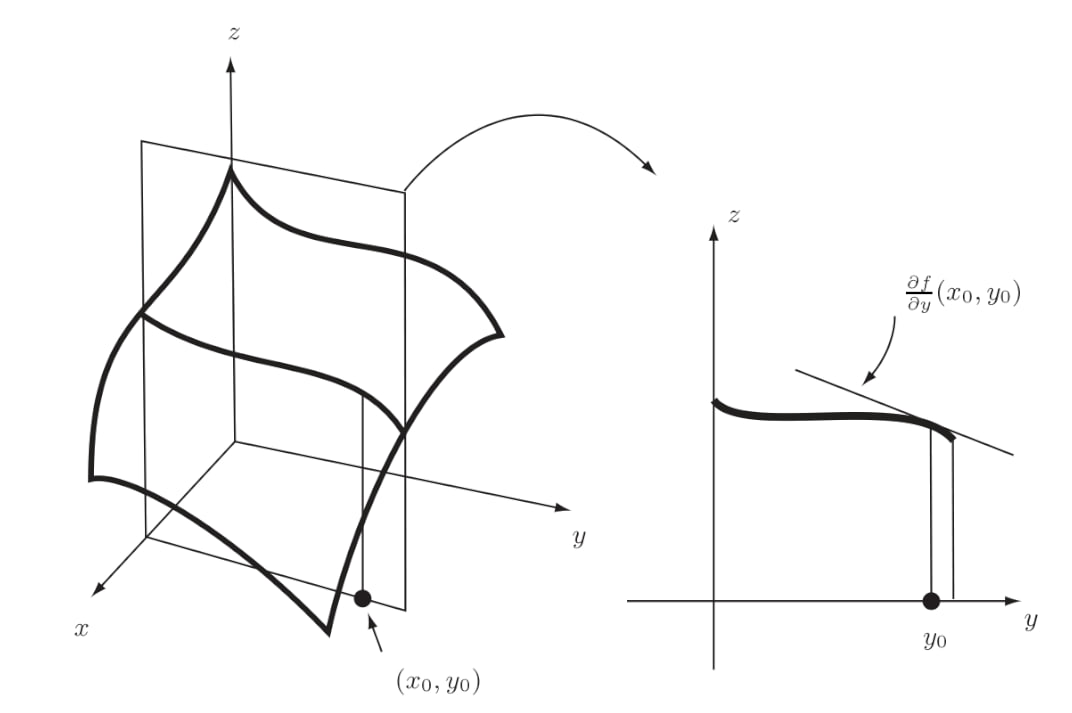
\includegraphics[scale = 0.6]{images/partial_deri.jpg}
    \caption{Мы рассекли график $z =f(x,y)$ плоскостью, параллельной плоскости $yz$, через точку $(x_0,y_0,0)$. Тогда мы получаем кривую, которая представляется какой-то функцией от $y$, и её наклон и есть $\frac{\partial f}{\partial y}(x_0,y_0)$.}
    \label{fig:enter-label}
\end{figure}

\subsection{Построение касательной плоскости}

С другой стороны, мы можем пойти дальше и рассечь этот же график, но уже не параллельной ни плоскости $yz$, ни плоскости $xz$. Как тогда вычислить наклон?

Чтобы ответить на этот вопрос, мы рассмотрим множество всех прямых, которые касаются графика в точке $(x_0, y_0, f(x_0,y_0))$. Такое множество мы называем \textit{касательной плоскостью} к графику $z = f(x,y).$

Уравнение плоскости, которая проходит через точку $(0,0,0)$, имеет вид $z = Ax + By$. Тогда сдвинув эту плоскость к точке $(x_0, y_0, f(x_0,y_0))$, мы получим тогда такое уравнение плоскости: $z - f(x_0,y_0) = A(x-x_0) + B(y-y_0)$. Осталось найти коэффициенты $A,B$, чтобы эта плоскость стала касательной. Пересечём эту плоскость с плоскостью $y=y_0$, в результате мы получаем прямую $z(x, y_0) - f(x_0,y_0) = A(x-x_0)$, тогда потребовав, чтобы эта прямая была касательной, мы получаем, что $A = \frac{\partial f}{\partial x}(x_0,y_0)$. Аналогично находим $B = \frac{\partial f}{\partial y}(x_0,y_0)$.

Итак, мы получаем следующее определение
\begin{definition}
 Пусть задана поверхность $M$ уравнением $z  = f(x,y)$, рассмотрим точку $P=(x_0,y_0,z_0)$ на поверхности $M$. Пусть существуют частные производные $\frac{\partial f}{\partial x}(x_0,y_0)$, $\frac{\partial f}{\partial y}(x_0,y_0)$. Тогда множество точек удовлетворяющих уравнению 
 \[
z - f(x_0,y_0) = \left.\frac{\partial f}{\partial x}\right|_{(x_0,y_0)} (x-x_0) + \left.\frac{\partial f}{\partial y}\right|_{(x_0,y_0)} (y-y_0)
\]
называется \textit{касательной плоскостью} к поверхности $M$ в точке $P$, и обозначается так $T_PM$.
\end{definition}



\subsection{Базис касательной плоскости}
Нам удобно принять слудующие обозначения. Пусть $P = (x_0,y_0,z_0)$ принадлежит поверхности $M : =\{(x,y,z)\, : \, z  = f(x,y) \} $, тогда $z_0 = f(x_0,y_0)$. Пусть $p: = (x_0,y_0)$, тогда $P = (p, f(p))$.

Следующая теорема описывает касательную плоскость в теримнах базиса.

\begin{theorem}
 Касательная плоскость $T_PM$ к поверхности $M: = \{(x,y,z)\, : \, z  = f(x,y) \}$ в точке $P= (x_0,y_0,z_0)$, как векторное пространство может быть представлено в виде
 \[
 T_PM \cong \mathrm{Span}_\mathbb{R}(\m{v}_x, \m{v}_y),
 \]
 где
 \[
  \m{v}_x : = \bigl( 1,0, f'_x(p) \bigr)^\top, \qquad  \m{v}_y : = \bigl( 0,1, f'_y(p) \bigr)^\top
\]
и более того эти векторы образуют базис $T_PM.$
\end{theorem}
\begin{proof}
 
Сохраним прежние обозначения и рассмотрим теперь произвольную точку $P_1(x_1,y_1,z_1)$, возникаем вектор $\m{h}: = (x_1 - x_0, y_1-y_0, z_1-z_0)^\top$. Мы хотим понять, когда этот вектор будет лежать в касательной плоскости $T_PM.$ Для краткости, мы примем обозначения $h_1: = x_1 - x_0,$, $h_2: = y_1- y_0$, $h_3: = z_1 - z_0$, таким образом $\m{h} = (h_1,h_2,h_3)^\top$.

Далее, согласно определению касатальной плоскости, $\m{h} \in T_pM$ тогда и только тогда, когда 
 \[
z_1 - f(x_0,y_0) = f_x'(p) (x_1-x_0) + f'_y(p) (y_1-y_0)
\]
или в новых обозначениях
\[
 h_3 = f_x'(p) \cdot h_1 + f'_y(p) \cdot h_2.
\]

Таким образом, имеем
\[
 \m{h} = \begin{pmatrix}
     h_1 \\ h_2 \\h_3
 \end{pmatrix} = \begin{pmatrix}
     h_1 \\ h_2 \\ f_x'(p) \cdot h_1 + f'_y(p) \cdot h_2
 \end{pmatrix} = \begin{pmatrix}
     h_1 \\ 0 \\ f_x'(p) \cdot h_1
 \end{pmatrix} + \begin{pmatrix}
     0 \\ h_2 \\ f'_y(p) \cdot h_2
 \end{pmatrix} = h_1 \begin{pmatrix}
     1 \\ 0 \\ f'_x(p)
 \end{pmatrix} + h_2 \begin{pmatrix}
     0 \\ 1 \\ f'_y(p)
 \end{pmatrix}
\]
что и означает,
 \[
 T_PM \cong \mathrm{Span}_\mathbb{R}(\m{v}_x, \m{v}_y),
 \]
 где
 \[
  \m{v}_x : = \bigl( 1,0, f'_x(p) \bigr)^\top, \qquad  \m{v}_y : = \bigl( 0,1, f'_y(p) \bigr)^\top.
\]

Допустим что имеются такие числа $\alpha, \beta$, что $\alpha \cdot\m{v}_x+ \beta \cdot \m{v}_y = \m{0}$.

Имеем
\[
 \alpha \cdot\m{v}_x+ \beta \cdot \m{v}_y =  \alpha \begin{pmatrix}
     1 \\ 0 \\ f'_x(p)
 \end{pmatrix} + \beta \begin{pmatrix}
     0 \\ 1 \\ f'_y(p) \end{pmatrix} = \begin{pmatrix}
        \alpha \\ \beta \\ \alpha \cdot f_x'(p) + \beta \cdot f'_y(p)
     \end{pmatrix} = \begin{pmatrix}
         0\\0\\0
     \end{pmatrix}
\]
откуда $\alpha = \beta = 0$, \textit{т.е.,} векторы $\m{v}_x$, $\m{v}_y$ линейно неависимы. Это завершаешт доказательство.
\end{proof}


\section{Производная по направлению}
Вернёмся ещё раз к предыдущему рисунку. Введём обозначения. Пусть $P$ -- вертикальная плоскость, проходящая через точку $(x_0,y_0)$. Пусть $\ell$ -- прямая, по которой $P$ пересекает плоскость $xy$. Касательную прямую к кривой, которую высекает плоскость $P$, мы обозначим через $L$. Касательная плоскость в точке $(x_0,y_0, f(x_0,y_0))$ пусть будет $T$. Далее, рассмотрим вектор $\m{v}$, который лежит на $\ell$, выходит из точки $(x_0,y_0)$ и кончается в $(x_0+a, y_0 +b)$, \ie имеет координаты $(a,b)$.

\begin{figure}[h!]
    \centering
    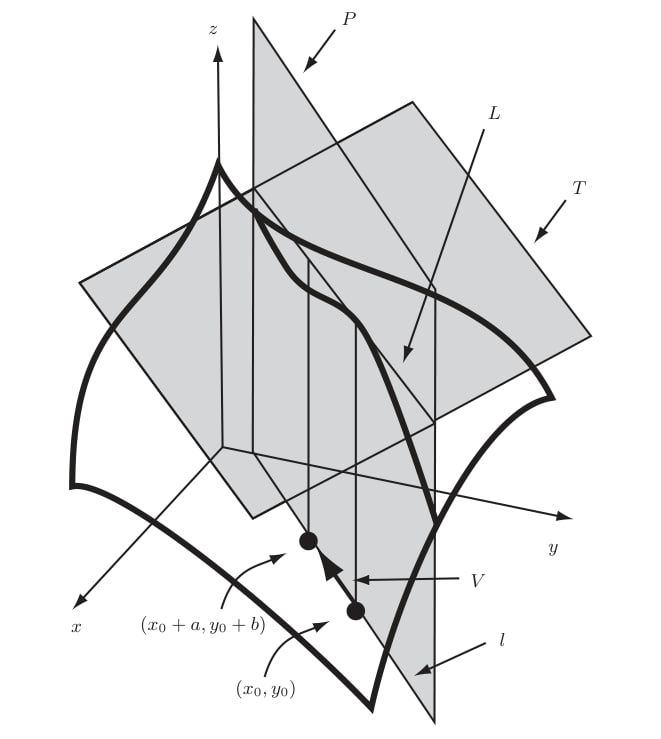
\includegraphics[scale =0.7]{images/direction_der2.jpg}
    \caption{Caption}
    \label{fig:enter-label}
\end{figure}



Имеем
\begin{eqnarray*}
    T(x_0 + a, y_0 + b) - T(x_0,y_0) &=& \left.\frac{\partial f}{\partial x}\right|_{(x_0,y_0)} (x_0 +a-x_0) + \left.\frac{\partial f}{\partial y}\right|_{(x_0,y_0)} (y_0 +b-y_0) \\
    &=& a\left.\frac{\partial f}{\partial x}\right|_{(x_0,y_0)} + b\left.\frac{\partial f}{\partial y}\right|_{(x_0,y_0)} \\
    &=& \langle \m{v} , \nabla f (x_0, y_0) \rangle
\end{eqnarray*}




Тогда, чтобы вычислить наклон, нужно потребовать, чтобы один из катетов в прямоугольном треугольнике был равен $1$, таким образом, если $a^2 + b^2 = 1$, то искомый наклон и есть число $\langle \m{v} , \nabla f (x_0, y_0) \rangle.$

Итак мы получаем следующее
\begin{definition}
    Пусть дана точка $\m{p} \in \mathbb{R}^n$, вектор $\m{v}\in \mathbb{R}^n$ и пусть $f:\mathbb{R}^n \to \mathbb{R}$ -- функция. Тогда \textit{производная по направлению $\m{v}$ вычисленная в точке $\m{p}$} есть выражение вида
    \[
     (\nabla_\m{v}f)(\m{p}): = \frac{1}{\| \m{v}\|} (\mathrm{d}f)_\m{p} \m{v},
    \]
\end{definition}
где справа стоит умножение матриц. А именно, так как
\[
 (\mathrm{d}f)_\m{p} = \begin{pmatrix}
     f'_{x_1}(\m{p}) & \ldots & f'_{x_n}(\m{p})
 \end{pmatrix} \in \mathrm{Mat}_{1\times n}(\mathbb{R}),
\]
то получаем
\[
 \boxed{
 (\nabla_\m{v}f)(\m{p}) =\frac{1}{\|\m{v}\|} \left(  f'_{x_1}(\m{p})v_1 + \cdots + f'_{x_n}(\m{p}) v_n\right).
 }
\]

\section{Необходимые и достаточные условия дифференцируемости}

\subsection{Необходимые условия}

Что касается необходимых условия дифференцируемости, то мы их уже знаем. Но для удобства мы сделаем из этого следующую теорему:



\begin{theorem}
    Если функция $f:\mathbb{R}^n \to \mathbb{R}$ дифференцируема на каком-то открытом $\mathscr{U} \subseteq \mathbb{R}^n$ или в фиксированной точке $\m{x}$, то она имеет в этой точке частные производные по всем переменным.
\end{theorem}

\begin{proof}
   Пусть $f:\mathbb{R}^n \to \mathbb{R}$, дифференцируемая на каком-то открытом $\mathscr{U} \subseteq \mathbb{R}^n$ или в фиксированной точке $\m{x}$. Тогда её дифференциал $(\mathrm{d}f)_\m{x}$ в точке $\m{x}$ задаётся матрицей размера $n\times 1$, $(\mathrm{d}f)_\m{x} = \begin{pmatrix}
    a_1 & \ldots & a_n
\end{pmatrix}$, где все $a_i$ есть функции от $\m{x}$. Наша цель -- найти эти $a_i$. Пусть $\m{h} = (h_1, \ldots, h_n)^\top \in \mathscr{U} \subseteq \mathbb{R}^n$, тогда получаем
\begin{eqnarray*}
    f(\m{x} + \m{h}) - f(\m{x}) &=& (\mathrm{d}f)_\m{x}(\m{h}) + o(||\m{h}||) \\
    &=& \begin{pmatrix}
        a_1 & \ldots & a_n
    \end{pmatrix} \begin{pmatrix}
        h_1 \\ \vdots \\ h_n  \end{pmatrix} + o(||\m{h}||) \\
        &=& a_1h_1 + \cdots + a_nh_n + o(||\m{h}||).
\end{eqnarray*}

Видно, что $a_i$ не зависит от координат вектора $\m{h}$ кроме $h_i$ \ie чтобы найти $a_i$, нам достаточно рассмотреть вектор $\m{h}_i = h_i \m{e}_i$, где $\m{e}_i$ -- базисный вектор. В таком случае, $||\m{h}_i|| = |h_i|$, и тогда для каждого $1 \le i \le n$ мы получаем
\[
 f(\m{x} + h_i \m{e}_i) - f(\m{x}) = a_ih_i + o(|h_i|),
\]
таким образом, 
\[
 a_i = \lim_{h_i \to 0} \frac{f(\m{x} + h_i \m{e}_i) - f(\m{x})}{h_i},
\]
такое выражение называется \textit{частной производной функции по переменной $x_i$} и обозначается либо как $\frac{\partial f}{\partial x_i}$, либо как $f'_{x_i}$, \ie 
\[
 \frac{\partial f}{\partial x_i}: = \lim_{h_i \to 0} \frac{f(\m{x} + h_i \m{e}_i) - f(\m{x})}{h_i},
\]
если же мы хотим знать её значение в точке $\m{x}_0$, то получаем
\[
 \frac{\partial f}{\partial x_i}(\m{x}_0): = \lim_{h_i \to 0} \frac{f(\m{x}_0 + h_i \m{e}_i) - f(\m{x}_0)}{h_i}.
\]
\end{proof}


Таким образом, в случае функции $f:\mathbb{R}^n \to \mathbb{R}$, дифференциал в точке $\m{x}_0$ находится по формуле
\[
 (\mathrm{d}f)_{\m{x}_0}: = \begin{pmatrix}
     \frac{\partial f}{\partial x_1}(\m{x}_0) & \ldots & \frac{\partial f}{\partial x_n}(\m{x}_0)
 \end{pmatrix}.
\]

\subsection{Достаточные условия дифференцируемости}

\begin{theorem}
Если все частные производные \( \frac{\partial f}{\partial x_i} \) существуют в окрестности \( \mathbf{a} \) и непрерывны в \( \mathbf{a} \), то \( f \) дифференцируема в \( \mathbf{a} \).    
\end{theorem}


\begin{proof} Для простоты мы начнём со случая двух переменных.

Итак, пусть функция \( f: \mathbb{R}^2 \to \mathbb{R} \) имеет непрерывные частные производные \( \frac{\partial f}{\partial x} \) и \( \frac{\partial f}{\partial y} \) в окрестности $\mathscr{U}$ точки \( \mathbf{a} = (x_0, y_0) \). Покажем что \( f \) дифференцируема в точке \( \mathbf{a} \).

\begin{figure}[h!]
    \centering
     \begin{tikzpicture}[>=Stealth, scale=1.2]
    % Координатные оси
    \draw[->] (-1,0) -- (6,0) node[below] {$x$};
    \draw[->] (0,-1) -- (0,5) node[left] {$y$};
    
    % Область U (светло-серый круг)
    \fill[lightgray!30] (3.5,2.5) circle (2cm);
    \node at (3,4) {$\mathscr{U}$};
    
    % Координатные линии и подписи для точки a+h
    \draw[dashed] (5,0) -- (5,3) -- (0,3);
    \filldraw (5,3) circle (1.5pt) node[above right] {$\mathbf{a} + \mathbf{h}$};
    
    % Вектор h и отрезки
    \draw[blue, thick] (3,2) -- node[midway, below] {$I_1$} (5,2);
    \draw[red, thick] (5,2) -- node[midway, right]  {$I_2$} (5,3);
    
    % Подпись вектора h
    %\node at (4.5,1.5) {$\mathbf{h} = (h_1, h_2)$};
    
    % Деления на осях
    \foreach \x in {1,...,5}
        \draw (\x,0.1) -- (\x,-0.1) node[below] {};
    \foreach \y in {1,...,4}
        \draw (0.1,\y) -- (-0.1,\y) node[left] {};
        
    %подписи координат
    \draw(3,0) node [below]{$x_0$};
    \draw(5,0) node [below]{$x_0+h_1$};
    \draw(0,2) node [left]{$y_0$};
    \draw(0,3) node [left]{$y_0+h_2$};

     % Координатные линии и подписи для точки a
    \draw[dashed] (3,0) -- (3,2) -- (0,2);
    \filldraw (3,2) circle (1.5pt) node[below left] {$\mathbf{a}$};    
\end{tikzpicture}
    \caption{В окрестности $\mathscr{U}$ точки $\m{a}$ мы имеем два отрезка, ограничения на которых мы получаем функции от одной координаты.}
    \label{fig:enter-label}
\end{figure}

Возьмём вектор \( \mathbf{h} = (h_1, h_2) \) такой, что $\m{a+h} \in \mathscr{U}$, тогда получаем два отрезка
\[
 I_1: = [ (x_0,y_0), (x_0 + h_1, y_0) ], \qquad I_2: = [ (x_0+h_1,y_0), (x_0+h_1, y_0+h_2) ],
\]
которые лежат в $\mathscr{U}$. Согласно условию, и определению частных производных, функции\footnote{это уже функции от одной переменной} $f_1: = f|_{I_1}$, $f_2: = f|_{I_2}$ дифференцируемы на отрезках $I_1, I_2$.

Тогда, согласно теореме Лагранжа \ref{Langrange}, существуют числа \( \theta_1, \theta_2 \in (0,1) \) такие, что
\begin{eqnarray*}
    f_1(x_0 + h_1, y_0) - f_1(x_0, y_0) &=& f'_1(x_0+\theta_1h_1, y_0)h_1,\\
    f_2(x_0 +h_1, y_0+h_2) - f_2(x_0+h_1, y_0) &=& f'_2(x_0 + h_1, y_0+\theta_2h_2)h_2.
\end{eqnarray*}

Согласно определению частных производных, это можно записать так

\begin{eqnarray*}
    f_1(x_0 + h_1, y_0) - f_1(x_0, y_0) &=& f'_x(x_0+\theta_1h_1, y_0)h_1,\\
    f_2(x_0 +h_1, y_0+h_2) - f_2(x_0+h_1, y_0) &=& f'_y(x_0 + h_1, y_0+\theta_2h_2)h_2.
\end{eqnarray*}

Тогда имеем

\begin{eqnarray*}
     f(\mathbf{a} + \mathbf{h}) - f(\mathbf{a}) &=& f(x_0 + h_1, y_0 + h_2) - f(x_0, y_0) \\
     &=& \Bigl( f(x_0 + h_1, y_0 + h_2) - f(x_0 + h_1, y_0) \Bigr)  + \Bigl(f(x_0 + h_1, y_0) - f(x_0, y_0)\Bigr)\\
     &=&f'_y(x_0 + h_1, y_0+\theta_2h_2)h_2 + f'_x(x_0+\theta_1h_1, y_0)h_1. 
\end{eqnarray*}

В более удобном виде это можно записать так
\[
 f(\mathbf{a} + \mathbf{h}) - f(\mathbf{a}) = f'_x(\m{a} + \theta_1 h_1 \m{e}_1)h_1 + f_y'(\m{a} + h_1\m{e}_1 + \theta_2 h_2 \m{e}_2)h_2.
\]

Имеем
\begin{eqnarray*}
    f(\mathbf{a} + \mathbf{h}) - f(\mathbf{a}) &=& f'_x(\m{a} + \theta_1 h_1 \m{e}_1)h_1 + f_y'(\m{a} + h_1\m{e}_1 + \theta_2 h_2 \m{e}_2)h_2 \\
    && + \Bigl( f'_x(\m{a})h_1 + f_y'(\m{a})h_2 \Bigr) - \Bigl(f'_x(\m{a})h_1 + f_y'(\m{a})h_2 \Bigr)
\end{eqnarray*}

Запишем это выражение следующим образом

\[
    f(\mathbf{a} + \mathbf{h}) - f(\mathbf{a}) = \underbrace{f'_x(\mathbf{a})h_1 + f'_y(\mathbf{a})h_2}_{\mathrm{d}f_\m{a}(\mathbf{h})} + R(\mathbf{h})
    \]
где
  \[
  R(\mathbf{h}) := \Bigl(f_x'(\m{a}+ \theta_1 h_1) - f_x'(\mathbf{a})\Bigr)h_1 + \Bigl(f_y'(\m{a} + h_1\m{e}_1 + \theta_2 h_2 \m{e}_2) - f'_y(\mathbf{a})\Bigr)h_2.
 \]

Покажем, что $R(\m{h}) = o(\|\m{h}\|)$, при $\m{h} \to \m{0}$. Действительно, так как $|h_i| \le \max \{ |h_1|,\ldots, |h|_n \}$, тогда, согласно неравенству Леммы \ref{m<d<M},
\[
\max_{1 \le k \le n} |h_k| \le \sqrt{\sum_{k=1}^n h_k^2} \le \sqrt{n} \max_{1\le k \le n} |h_k|,
\]
получаем $\frac{h_i}{\|\m{h}\|} \le 1$. Тогда имеем

\begin{eqnarray*}
  \left| \frac{R(\mathbf{h})}{\|\mathbf{h}\|} \right| &=& \frac{1}{\|\m{h}\|} \left| \Bigl(f_x'(\m{a}+ \theta_1 h_1) - f_x'(\mathbf{a})\Bigr)h_1 + \Bigl(f_y'(\m{a} + h_1\m{e}_1 + \theta_2 h_2 \m{e}_2) - f'_y(\mathbf{a})\Bigr)h_2 \right| \\
  &\leq& \frac{|h_1|}{\|\mathbf{h}\|}  \cdot \left|f_x'(\m{a}+ \theta_1 h_1) - f_x'(\mathbf{a}) \right|  + \frac{|h_2|}{\|\mathbf{h}\|}  \cdot \left|f_y'(\m{a} + h_1\m{e}_1 + \theta_2 h_2 \m{e}_2) - f'_y(\mathbf{a}) \right|  \\
  &\le & \left| \Bigl(f_x'(\m{a}+ \theta_1 h_1) - f_x'(\mathbf{a})\Bigr) \right|  +  \left|f_y'(\m{a} + h_1\m{e}_1 + \theta_2 h_2 \m{e}_2) - f'_y(\mathbf{a}) \right|
\end{eqnarray*}

Так как при $\m{h} \to \m{0}$, имеем $h_1,h_2 \to 0$, то в силу непрерывности частных производных имеем
\[
 \lim_{h_1,h_2 \to 0} \left|  f_x'(\m{a}+ \theta_1 h_1) - f_x'(\mathbf{a}) \right| =0,  \qquad \lim_{h_1,h_2 \to 0} \left|f_y'(\m{a} + h_1\m{e}_1 + \theta_2 h_2 \m{e}_2) - f'_y(\mathbf{a}) \right| = 0
\]
\textit{т.е.,} $R(\m{h}) = o(\|\m{h}\|)$, при $\m{h} \to \m{0}$. Это завершает доказательство в случае двух переменных.

В общем случае, мы тогда можем аналогично рассмотреть отрезки 


\[
    f(\mathbf{a} + \mathbf{h}) - f(\mathbf{a}) = \sum_{i=1}^n \left[ f(\mathbf{a} + \mathbf{h}^{(i)}) - f(\mathbf{a} + \mathbf{h}^{(i-1)}) \right],
    \]
    где \( \mathbf{h}^{(i)} = (h_1, \dots, h_i, 0, \dots, 0) \).

    \item Применяем теорему Лагранжа:
    \[
    f(\mathbf{a} + \mathbf{h}^{(i)}) - f(\mathbf{a} + \mathbf{h}^{(i-1)}) = h_i \frac{\partial f}{\partial x_i}(\mathbf{a} + \mathbf{c}_i),
    \]
    где \( \mathbf{c}_i: = \m{h}^{(i-1)} + \theta_ih_i \m{e}_i \) — точка на соответствующем отрезке.

    \item Линейная часть и остаток:
    \[
    f(\mathbf{a} + \mathbf{h}) - f(\mathbf{a}) = \nabla f(\mathbf{a}) \cdot \mathbf{h} + \underbrace{\sum_{i=1}^n h_i \left( \frac{\partial f}{\partial x_i}(\mathbf{a} + \mathbf{c}_i) - \frac{\partial f}{\partial x_i}(\mathbf{a}) \right)}_{R(\mathbf{h})}.
    \]

    \item Оценка остатка:
    \[
    |R(\mathbf{h})| \leq \sum_{i=1}^n |h_i| \cdot \epsilon \leq \epsilon \|\mathbf{h}\|_1 = o(\|\mathbf{h}\|).
    \]
\end{proof}

\section{Дифференциал композиции}


\subsection{Непрерывность линейных отображений}

Напомним, что линейное отображение $L: \mathbb{R}^n \to \mathbb{R}^m$ -- это такое отображение, что
\[
 L(\alpha \m{v} + \beta \m{u}) = \alpha L(\m{v}) + \beta L(\m{u}),
\]
для любых $\m{v}, \m{u} \in \mathbb{R}^n$, $\alpha,\beta \in \mathbb{R}$.

Заметим, что 
\[
 L(\m{0}_n) = \m{0}_m,
\]
где $\m{0}_k$ -- нулевой вектор векторного пространства $\mathbb{R}^k$.


\begin{definition}
    Говорят, что линейное отображение $L: \mathbb{R}^n \to \mathbb{R}^m$ ограничено, если существует такое $K \ge 0$, что для любого $\m{v} \in \mathbb{R}^n$, $|| L(\m{v}) || \le K ||\m{v}||.$
\end{definition}

\begin{proposition}\label{contous_of_linear}
    Пусть $L: \mathbb{R}^n \to \mathbb{R}^m$ -- линейное отображение. Тогда следующие утверждения равносильны:
    \begin{enumerate}
        \item $L$ -- непрерывно.
        \item $L$ -- непрерывно в нуле.
        \item Существует такое $C > 0$, что $|| L(\m{v})| \le C ||\m{v}||$ для любого $\m{v} \in \mathbb{R}^n$
    \end{enumerate}
\end{proposition}
\begin{proof}
(1) $\Longrightarrow$ (2). Это просто следует из того, что если $L$ непрерывно, то оно непрерывно во всех точках $\mathbb{R}$, в частности и в нуле тоже.

(2) $\Longrightarrow$ (3). Если $L$ непрерывно в нуле, то это значит, что для любого $\varepsilon >0$ можно всегда найти такое $\delta>0$, что из $||\m{h}|| <\delta$ будет следовать $||L(\m{h})|| <\varepsilon$. Пусть $\varepsilon = 1$, тогда мы всегда найдём такой $\delta>0$, что если $|| \m{h} || < \delta$, то $|| L(\m{h})|| < 1$. Зафиксируем такое $\delta.$

Возьмём теперь произвольный ненулевой вектор\footnote{Аксиома Выбора позволяет.} $\m{v}$, тогда имеем
\begin{eqnarray*}
 || L(\m{v}) || &=& \left\| \frac{2}{\delta} || \m{v} || L\left(  \frac{\delta \m{v}}{2 || \m{v} ||}\right) \right\| \\
 &=&  \frac{2}{\delta} || \m{v}|| \cdot \left\| L\left(  \frac{\delta \m{v}}{2 || \m{v} ||}\right) \right\| < \frac{2}{\delta} || \m{v}||
\end{eqnarray*}
потому что 
\[
 \left\|\frac{\delta \m{v}}{2 || \m{v} ||} \right\| = \frac{\delta}{2} < \delta,
\]
и так как $\delta$ фиксировано, мы получаем требуемое.

(3) $\Longrightarrow$ (1). Имеем
\[
 || L(\m{v}) - L(\m{u}) || = || L(\m{v} - \m{u}) || \le K || \m{u} - \m{v} ||,
\]
тогда если $||\m{u} - \m{v}|| < \delta$, то $|| L(\m{v}) - L(\m{u}) ||< K \delta$,
поэтому для любого $\varepsilon >0$, если мы положим, что $0<\delta < \frac{\varepsilon}{K}$, то мы и получаем непрерывность $L$.
\end{proof}




\begin{lemma}\label{linear_is_contious}
    Любое линейное отображение $L: \mathbb{R}^n \to \mathbb{R}^m$ непрерывно. 
\end{lemma}
\begin{proof}
Пусть $L$ задаётся матрицей $(a_{i,j})_{1\le i \le n, 1 \le j \le m}$, тогда

\[
 L(\m{v}) = \begin{pmatrix}
     a_{11} & \ldots & a_{1n} \\
     \vdots & \ddots & \vdots \\
     a_{m1} & \ldots & a_{mn}
 \end{pmatrix}   \begin{pmatrix}
     v_1 \\ \vdots \\ v_n
 \end{pmatrix} = \begin{pmatrix}
     a_{11}v_1 + \cdots + a_{1n}v_n \\
     \vdots \\
     a_{m1}v_1 + \cdots + a_{mn}v_n 
 \end{pmatrix} = (u_1, \ldots, u_m)^\top =:\m{u} \in \mathbb{R}^m,
\] 
тогда
\begin{eqnarray*}
    ||L(\m{v})|| &=& ||\m{u}|| \\
    &=& \sqrt{(a_{11}v_1 + \cdots + a_{1n}v_n)^2 + \cdots + (a_{m1}v_1 + \cdots + a_{mn}v_n)^2} \\
    &\le & \sqrt{ m } \max_{1 \le k \le m} \left| a_{k1}v_1 + \cdots + a_{kn}v_n  \right| \\
    &\le & \sqrt{ m } \max_{1 \le k \le m} \left( |a_{k1}| \cdot |v_1| + \cdots + |a_{kn}| \cdot |v_n| \right) \\
    &\le & \sqrt{ m } \max_{1 \le k \le m} \left(|a_{k1}| \cdot || \m{v}|| + \cdots + |a_{kn}| \cdot || \m{v}||  \right) \\
    &=& \sqrt{ m } \max_{1 \le k \le m}\left(|a_{k1}|  + \cdots + |a_{kn}|   \right) \cdot || \m{v}|| \\
    &=& K || \m{v}||,
\end{eqnarray*}
где $K: = \sqrt{ m } \max_{1 \le k \le m}\left(|a_{k1}|  + \cdots + |a_{kn}|   \right)$, тогда по Предложению \ref{contous_of_linear} оно непрерывно. 
\end{proof}


\subsection{Дифференциал композиции}


\begin{theorem}\label{d(FG)}
    Пусть $F: \mathbb{R}^n \to \mathbb{R}^k$ дифференцируема в $\m{a} \in \mathbb{R}^n$, $G: \mathbb{R}^k \to \mathbb{R}^m$ дифференцируемо в $\m{b}= F(\m{a})$. Тогда $H: = G \circ F :\mathbb{R}^n \to \mathbb{R}^m$ дифференцируемо в $\m{a}$ и 
    \[
     (\mathrm{d}H)_\m{a} = (\mathrm{d}G)_{\m{b}} \cdot (\mathrm{d}F)_\m{a},
    \]
    где подразумевается обычное умножение матриц.
\end{theorem}


\begin{proof}

 Так как отображения дифференцируемо, мы имеем
 \[
  F(\m{a} + \m{h}) - F(\m{a}) = (\mathrm{d}F)_\m{a}(\m{h}) + \alpha(\m{h}) \cdot || \m{h}||,
 \] 
 и
 \[
  G(F(\m{a}) + \m{v})) - G(F(\m{a})) = (\mathrm{d}G)_{F(\m{a})}(\m{v}) + \beta(\m{v}) ||\m{v}||
 \]
где $\lim_{\m{h} \to \m{0}_n} \alpha (\m{h}) = \m{0}_k$, $\lim_{\m{v} \to \m{0}_k} \beta (\m{v}) = \m{0}_m$.

Мы можем положить $\beta(\m{0}_k) = \m{0}_m$ или доопределить её таким образом, видно, что на равенства это не повлияет. Тем самым, $\beta$ может считаться непрерывной в $\m{0}_k$.

Пусть $\m{v}: = F(\m{a} + \m{h}) - F(\m{a})$, тогда $G(F(\m{a}) + \m{v})) - G(F(\m{a}) = G(F(\m{a}+\m{h})) -G(F(\m{a}))$. 

Имеем

\begin{eqnarray*}
    G(F(\m{a}+\m{h})) -G(F(\m{a})) &=& (\mathrm{d}G)_{F(\m{a})}\bigl(F(\m{a}+ \m{h}) - F(\m{a})\bigr)  \\
    &+& \beta\Bigl( F(\m{a} +\m{h}) - F(\m{a}) \Bigr) \cdot || F(\m{a} + \m{h}) - F(\m{a})|| \\
    &=& (\mathrm{d}G)_{F(\m{a})} \Bigl( (\mathrm{d}F)_\m{a}(\m{h}) + \alpha(\m{h}) \cdot || \m{h}||\Bigr) \\
    &+& \beta \Bigl(F(\m{a} + \m{h}) - F(\m{a})\Bigr) \cdot \Bigl\| (\mathrm{d}F)_\m{a}(\m{h}) + \alpha(\m{h}) \cdot || \m{h}|| \Bigr\|
\end{eqnarray*}
из-за линейности $(\mathrm{d}G)_{F(\m{a})}$ получаем
\begin{eqnarray*}
    G(F(\m{a}+\m{h})) -G(F(\m{a})) &=&\Bigl((\mathrm{d}G)_{F(\m{a})} \circ (\mathrm{d}F)_\m{a}\Bigr) (\m{h}) + (\mathrm{d}G)_{F(\m{a})}((\alpha(\m{h})) \cdot || \m{h}|| \\
    &+& \beta \Bigl(F(\m{a} + \m{h}) - F(\m{a}) \Bigr) \cdot \Bigl\| (\mathrm{d}F)_\m{a}(\m{h}) + \alpha(\m{h}) \cdot || \m{h}|| \Bigr\|     
\end{eqnarray*}
вынесем теперь $|| \m{h}||$, получаем
\begin{eqnarray*}
    G(F(\m{a}+\m{h})) -G(F(\m{a})) &=&\Bigl((\mathrm{d}G)_{F(\m{a})} \circ (\mathrm{d}F)_\m{a}\Bigr) (\m{h})\\
    &+&\left( (\mathrm{d}G)_{F(\m{a})}\bigl((\alpha(\m{h})\bigr) + \beta \Bigl(F(\m{a} + \m{h}) - F(\m{a}) \Bigr) \cdot \left\| \frac{(\mathrm{d}F)_\m{a}(\m{h})}{|| \m{h} ||} + \alpha(\m{h})  \right\| \right) || \m{h} ||.     
\end{eqnarray*}

Так как $(\mathrm{d}F)_\m{a}: \mathbb{R}^n \to \mathbb{R}^k$ линейно, то по Лемме \ref{linear_is_contious} и Предложению \ref{contous_of_linear} оно ограничено, то есть $|| (\mathrm{d}F)_\m{a})(\m{h}) || \le K ||\m{h}||$. Далее, так как $(\mathrm{d}G)_{F(\m{a})}: \mathbb{R}^k \to \mathbb{R}^m$ линейно, то по Лемме \ref{linear_is_contious} оно непрерывно, и так как мы положили, что $\beta$ непрерывна в $\m{0}_k$, тогда 
\begin{eqnarray*}
 \lim_{\m{h} \to \m{0}_n}(\mathrm{d}G)_{F(\m{a})}\bigl((\alpha(\m{h})\bigr) &=& (\mathrm{d}G)_{F(\m{a})}\bigl( \lim_{\m{h} \to \m{0}_n} (\alpha(\m{h})\bigr) = \m{0}_m,\\
 \lim_{\m{h} \to \m{0}_n} \beta \Bigl(F(\m{a} + \m{h}) - F(\m{a}) \Bigr) &=& \beta (\m{0}_k) = \beta(\m{0}_m). 
\end{eqnarray*}

Далее, 
\[
  \left\| \frac{(\mathrm{d}F)_\m{a}(\m{h})}{|| \m{h} ||} + \alpha(\m{h})  \right\| \le \left\| \frac{(\mathrm{d}F)_\m{a}(\m{h})}{|| \m{h} ||} \right\| + \| \alpha(\m{h}) \| \le K + \| \alpha(\m{h}) \|,
\]
так как $\lim_{\m{h} \to \m{0}_n}\alpha(\m{h}) = \m{0}_k$, то согласно Предложению \ref{xn->x=||xn||->||x||}, Теореме \ref{f<g=>lim}:
\[
 0 \le \lim_{\m{h} \to \m{0}_n}\left\| \frac{(\mathrm{d}F)_\m{a}(\m{h})}{|| \m{h} ||} + \alpha(\m{h})  \right\| =C \le K.
\]

Итак, пусть
\[
 \omega (\m{h}): = \lim_{\m{h} \to \m{0}_n}\left( (\mathrm{d}G)_{F(\m{a})}\bigl((\alpha(\m{h})\bigr) + \beta \Bigl(F(\m{a} + \m{h}) - F(\m{a}) \Bigr) \cdot \left\| \frac{(\mathrm{d}F)_\m{a}(\m{h})}{|| \m{h} ||} + \alpha(\m{h})  \right\| \right),
\]
тогда мы показали, что
\[
 \lim_{\m{h} \to \m{0}_n} \omega (\m{h}) = \m{0}_m. 
\]

Окончательно мы получили, что
\[
 G(F(\m{a}+\m{h})) -G(F(\m{a})) =\Bigl((\mathrm{d}G)_{F(\m{a})} \circ (\mathrm{d}F)_\m{a}\Bigr) (\m{h}) +   \omega (\m{h}) || \m{h} ||,
\]
что и доказывает утверждение.
\end{proof}

%\chapter{Высшие дифференциалы в $\mathbb{R}^n$}


\section{Дифференциалы высокого порядка}

Пусть дана функция $f: \mathbb{R}^n \to \mathbb{R}$ такая, что в открытом $\mathscr{U}$ у неё существуют все её частные производные $f_{x_i}' = \frac{\partial f}{\partial x_i}$. Пусть далее $\mathscr{V} \subseteq \mathscr{U}$ открыто, и пусть всюду в $\mathscr{V}$ её частные производные дифференцируемы, тогда мы получаем:
\begin{definition}
    Частные производные высокого порядка определяются как частные производные от частных производных, \ie
    \begin{eqnarray*}
        \frac{\partial^2 f}{\partial x_i \partial x_j} &:=& \frac{\partial }{\partial x_i}\left( \frac{\partial f}{\partial x_j} \right) = (f_{x_j}')'_{x_i} =: f''_{x_ix_j}. 
    \end{eqnarray*}
\end{definition}

\begin{mydanger}{\bf{!}}
    Выражение (если оно имеет смысл) $\frac{\partial f}{\partial x_i \partial x_j}$ называется \textit{смешанной производной}.
\end{mydanger}

\begin{lemma}\label{f''_xy}
    Для функции $f:\mathbb{R}^2 \to \mathbb{R}$ её смешанные производные $f''_{xy}(\m{a})$, $f''_{yx}(\m{a})$ в точке $\m{a} = (x_0,y_0)$ это пределы
\begin{eqnarray*}
    f''_{xy}(\m{a}) &=& \lim_{h\to 0} \lim_{k\to 0} \frac{f(x_0 + h, y_0 + k) - f(x_0 + h, y_0) - f(x_0,y_0 +k) + f(x_0,y_0)}{hk} \\
    f''_{yx}(\m{a}) &=& \lim_{k\to 0} \lim_{h\to 0} \frac{f(x_0 + h, y_0 + k) - f(x_0 + h, y_0) - f(x_0,y_0 +k) + f(x_0,y_0)}{hk}
\end{eqnarray*}
\end{lemma}

\begin{mydangerr}{\bf !}
    Обратите внимание на порядок вычисления пределов! Вовсе не обязательно что они должны совпадать.
\end{mydangerr}

\begin{proof}
Докажем только первую формулу, так как вторая формула доказывается совершенно аналогично. 

Итак, пусть $\m{a} = (x_0,y_0)$, тогда, по определению (\ref{partial_i(o)}), 
\begin{eqnarray*}
       \left. \frac{\partial^2 f}{\partial x \partial y}\right|_\m{a} &=& \left. \frac{\partial}{\partial x}\left( \frac{\partial f}{\partial y} \right) \right|_\m{a} := \lim_{h \to 0} \left( \frac{\frac{\partial f}{\partial y}(x_0+h, y_0) - \frac{\partial f}{\partial y}(x_0,y_0)  }{h}  \right).
\end{eqnarray*}

Теперь используя ещё раз определение производной, получаем
Пусть  
    \begin{eqnarray*}
       \left. \frac{\partial^2 f}{\partial x \partial y}\right|_\m{a}
       &=& \lim_{h \to 0}\left( \frac{ \lim\limits_{k\to 0} \dfrac{f(x_0+t, y_0 +k) -f(x_0+h,y_0)}{k}  - \lim\limits_{k\to 0} \dfrac{f(x_0,y_0+k) -f(x_0,y_0)}{k} } {h}  \right) \\
       &=& \lim_{h\to 0} \lim_{k \to 0} \dfrac{f(x_0+h, y_0 +k) -f(x_0+h,y_0) - f(x_0,y_0+k) +f(x_0,y_0)}{hk},
    \end{eqnarray*}
    что и требовалось доказать.
\end{proof}


\subsection{Теорема Шварца}


\begin{theorem}[\bf Шварц]
    Пусть $f:\mathbb{R}^2 \to \mathbb{R}$ имеет в окрестности $\mathscr{U}$ точки $\m{a} \in \mathbb{R}^2$ смешанные производные. Если эти производные непрерывны в этой точке, то они равны в этой точке, \textit{т.е.,}
    \[f''_{xy}(\m{a}) = f''_{yx}(\m{a}).
    \]
\end{theorem}

\begin{proof}
    Пусть $\m{a} = (x_0,y_0)$, рассмотрим приращение функции по переменным \( h \) и \( k \):  
   \[
   \Delta f := f(x_0+h, y_0+k) - f(x_0+h, y_0) - f(x_0, y_0+k) + f(x_0, y_0).
   \]

(1) Запишем \(\Delta f\) как разность приращений по \(y\):  
\[
\Delta f = \Bigl(f(x_0+h, y_0+k) - f(x_0+h, y_0)\Bigr) - \Bigl(f(x_0, y_0+k) - f(x_0, y_0)\Bigr).
\]  

К каждой скобке можно применить теорему Лагранжа \ref{Langrange}:
\begin{eqnarray*}
f(x_0+h, y_0+k) - f(x_0+h, y_0) &=& k \cdot f'_y(x_0+h, y_0 + \theta_1 k), \quad \theta_1 \in (0, 1)    \\
f(x_0, y_0+k) - f(x_0, y_0) &=& k \cdot f'_y(x_0, y_0 + \theta_2 k), \quad \theta_2 \in (0, 1).
\end{eqnarray*}

Тогда:  
\[
\Delta f = k \Bigl(f'_y(x_0+h, y_0 + \theta_1 k) - f'_y(x_0, y_0 + \theta_2 k)\Bigr).
\]

(2) Далее, имеем:
\begin{eqnarray*}
    \frac{\Delta f}{k} &=& f'_y(x_0+h, y_0 + \theta_1 k) - f'_y(x_0, y_0 + \theta_2 k) \\
    &=&f'_y(x_0+h, y_0 + \theta_1 k) - f'_y(x_0, y_0 + \theta_1 k) + f'_y(x_0, y_0 + \theta_1 k) - f'_y(x_0, y_0 + \theta_2 k) \\
    &=& \Bigl(f'_y(x_0+h, y_0 + \theta_1 k) - f'_y(x_0, y_0 + \theta_1 k)\Bigr) + \Bigl( f'_y(x_0, y_0 + \theta_1 k) - f'_y(x_0, y_0 + \theta_2 k) \Bigr).
\end{eqnarray*}


\begin{itemize}
\item[--] Применяем к первой скобке теорему Лагранжа \ref{Langrange}:  
\[
f'_y(x_0+h, y_0 + \theta_1 k) - f'_y(x_0, y_0 + \theta_1 k) = h \cdot f''_{yx}(x_0 + \theta_3 h, y_0 + \theta_1 k), \quad \theta_3 \in (0, 1).
\]
\item[--] Теперь применяем теорему Лагранжа \ref{Langrange} ко второй скобке:  
\[
f'_y(x_0, y_0 + \theta_1 k) - f'_y(x_0, y_0 + \theta_2 k) = (\theta_1 - \theta_2)k \cdot f''_{yy}(x_0, y_0 + \theta_4 k), \quad \theta_4 \in (0, 1).
\]
\end{itemize}

Подставим в выражение для \(\Delta f\):  
\[
\frac{\Delta f}{k} =h \cdot f''_{yx}(x_0 + \theta_3 h, y_0 + \theta_1 k) + (\theta_1 - \theta_2)k \cdot f''_{yy}(x_0, y_0 + \theta_4 k),
\]
или

\[
 \frac{\Delta f}{kh} =  f''_{yx}(x_0 + \theta_3 h, y_0 + \theta_1 k) + (\theta_1 - \theta_2)\frac{k}{h} \cdot f''_{yy}(x_0, y_0 + \theta_4 k)
\]


(3) Согласно условию, смешанные производные существуют и непрерывны, тогда используя лемму \ref{f''_xy}, предел $f''_{yx} = \lim_{k \to 0} \lim_{h \to 0} \frac{\Delta f}{hk}$ существует. Но тогда он существует для любого подмножества в окрестности точки $(0,0)$, поэтому мы можем, например, положить, $k = h^2$. В таком случае второе слагаемое стремится к нулю из-за непрерывности \(f''_{yy}\), а первое слагаемое стремится к \(f''_{yx}(x_0, y_0)\).

(4) Аналогично рассуждаем для другого порядка производных. Запишем \(\Delta f\) через приращения по \(x\):  
\[
\Delta(h, k) = \Bigl(f(x_0+h, y_0+k) - f(x_0, y_0+k)\Bigr) - \Bigl(f(x_0+h, y_0) - f(x_0, y_0)\Bigr).
\]  

Аналогично применяя теорему Лагранжа, получим:  
\[
\frac{\Delta f}{hk} = f''_{xy}(x_0 + \theta_5 h, y_0 + \theta_7 k) + (\theta_5 - \theta_6)\frac{h}{k} \cdot f''_{xx}(x_0 + \theta_8 h, y_0).
\]  
Устремим \(h, k \to 0\) так, что \(\frac{h}{k} \to 0\) (например, \(h = k^2\)). Второе слагаемое стремится к нулю, а первое —- к \(f''_{xy}(x_0, y_0)\).

Так как пределы \(\frac{\Delta f}{hk}\) при разных порядках вычисления по $h,k$ совпадают, то:  
\[
f''_{xy}(x_0, y_0) = f''_{yx}(x_0, y_0).
\]
Что и требовалось доказать.
\end{proof}

\subsection{Теорема Юнга}


**Теорема Юнга о равенстве смешанных производных** утверждает, что если функция \( f(x, y) \) имеет в окрестности точки \( (a, b) \) смешанные производные второго порядка \( f''_{xy} \) и \( f''_{yx} \), и эти производные непрерывны в точке \( (a, b) \), то они равны:  
\[
f''_{xy}(a, b) = f''_{yx}(a, b).
\]

**Доказательство:**

1. **Введение вспомогательной величины:**  
   Рассмотрим приращение функции для малых \( h \) и \( k \):  
   \[
   \Delta(h, k) = f(a + h, b + k) - f(a + h, b) - f(a, b + k) + f(a, b).
   \]  
   Поделим его на \( hk \):  
   \[
   \frac{\Delta(h, k)}{hk} = \frac{f(a + h, b + k) - f(a + h, b) - f(a, b + k) + f(a, b)}{hk}.
   \]

2. **Применение теоремы о среднем значении (сначала по \( x \), затем по \( y \)):**  
   - Определим функцию \( g(x) = f(x, b + k) - f(x, b) \). Тогда:  
     \[
     \Delta(h, k) = g(a + h) - g(a).
     \]  
     По теореме о среднем значении для \( g(x) \), существует \( \theta \in (0, 1) \), такое что:  
     \[
     g(a + h) - g(a) = h \cdot g'(a + \theta h) = h \left[ f'_x(a + \theta h, b + k) - f'_x(a + \theta h, b) \right].
     \]  
   - Теперь применим теорему о среднем значении к разности по \( y \). Существует \( \phi \in (0, 1) \), такое что:  
     \[
     f'_x(a + \theta h, b + k) - f'_x(a + \theta h, b) = k \cdot f''_{xy}(a + \theta h, b + \phi k).
     \]  
   - Таким образом:  
     \[
     \frac{\Delta(h, k)}{hk} = f''_{xy}(a + \theta h, b + \phi k).
     \]  
     При \( h, k \to 0 \) непрерывность \( f''_{xy} \) даёт:  
     \[
     \lim_{h, k \to 0} \frac{\Delta(h, k)}{hk} = f''_{xy}(a, b).
     \]

3. **Применение теоремы о среднем значении (сначала по \( y \), затем по \( x \)):**  
   - Определим функцию \( h(y) = f(a + h, y) - f(a, y) \). Тогда:  
     \[
     \Delta(h, k) = h(b + k) - h(b).
     \]  
     По теореме о среднем значении для \( h(y) \), существует \( \psi \in (0, 1) \), такое что:  
     \[
     h(b + k) - h(b) = k \cdot h'(b + \psi k) = k \left[ f'_y(a + h, b + \psi k) - f'_y(a, b + \psi k) \right].
     \]  
   - Применим теорему о среднем значении к разности по \( x \). Существует \( \xi \in (0, 1) \), такое что:  
     \[
     f'_y(a + h, b + \psi k) - f'_y(a, b + \psi k) = h \cdot f''_{yx}(a + \xi h, b + \psi k).
     \]  
   - Таким образом:  
     \[
     \frac{\Delta(h, k)}{hk} = f''_{yx}(a + \xi h, b + \psi k).
     \]  
     При \( h, k \to 0 \) непрерывность \( f''_{yx} \) даёт:  
     \[
     \lim_{h, k \to 0} \frac{\Delta(h, k)}{hk} = f''_{yx}(a, b).
     \]

4. **Заключение:**  
   Поскольку оба предела равны одному и тому же выражению \( \frac{\Delta(h, k)}{hk} \), получаем:  
   \[
   f''_{xy}(a, b) = f''_{yx}(a, b).
   \]  

**Условия теоремы существенны:** Непрерывность смешанных производных гарантирует, что пределы совпадают. Без неё равенство может нарушаться.




\begin{theorem}[Юнг]\label{Yong}
    Пусть у функции $f:\mathbb{R}^2 \to \mathbb{R}$ в окрестности в точке $\m{a} = (a_1,a_2)^\top$ существуют частные производные $f'_{x}$ и $f'_{y}$. Если эти частные производные дифференцируемы в точке $\m{a}$, то
    \[
     f''_{xy}(a_1,a_2) = f''_{yx}(a_1,a_2).
    \]
\end{theorem}

%Нужно сказать про отличие от предыдущей.






\section{Высшие дифференциалы}

\subsection{Общие замечания}

Рассмотрим отображение $F: \mathbb{R}^n \to \mathbb{R}^m$, которе мы будем, для простоты предполагать дифференцируемым всюду. Тогда для каждой точки $\m{p} \in \mathbb{R}^n$ у нас есть линейное отображение (=дифференциал) $(\mathrm{d}F)_{\m{p}}: \mathbb{R}^n\to \mathbb{R}^m$. 

Таким образом, мы получаем отображение
\[
 \mathrm{d}F: \mathbb{R}^n\to \mathrm{Hom}_\mathbb{R}(\mathbb{R}^n, \mathbb{R}^m) \qquad \m{p} \mapsto (\mathrm{d}F)_{\m{p}}.
\]

Так как линейные отображения из $\mathbb{R}^n$ в $\mathbb{R}^m$ -- это просто матрицы размера $m\times n$, а пространство матриц $\mathrm{Mat}_{m\times n}(\mathbb{R})$ есть векторное пространство, которое изоморфно $\mathbb{R}^{mn}$, то отображение $\mathrm{d}F$ это отображение между конечномерными векторными пространствами.

В силу эквивалентности норм на векторных пространствах (см. Лемму \ref{all_norma_are_=}), на пространстве $\mathrm{Hom}(\mathbb{R}^n, \mathbb{R}^m)$ можно рассмотреть евклидову норму. Всё это позволяет теперь поставить вопрос о дифференцируемости отображения $\mathrm{d}F$.

\begin{definition}
Если отображение
\[
 \mathrm{d}F: \mathbb{R}^n\to \mathrm{Hom}_\mathbb{R}(\mathbb{R}^n, \mathbb{R}^m) \qquad \m{p} \mapsto (\mathrm{d}F)_{\m{p}}
\]
дифференцируемо в точке $\m{a} \in \mathbb{R}$, то его дифференциал $(\mathrm{d}(\mathrm{d}F))_\m{a}$ называют \textit{вторым дифференциалом отображения $F$} вычисленный в точке $\m{a}$, при этом пишут $(\mathrm{d}^2F)_\m{a}.$ 

Таким образом, мы получаем отображения (если они существуют)
\[
 F:=\mathrm{d}^0F,\quad  \mathrm{d}F,\quad \mathrm{d}^2(F): = \mathrm{d}(\mathrm{d}F), \ldots, 
\]
среди которых $\mathrm{d}^k(F)$ при $k>1$ называются \textit{высшими дифференциалами.}
\end{definition}

Напомним что для векторных пространств $\m{V},\m{W}$ над полем $\Bbbk$, отображение $B:\m{V}\times \m{V} \to \m{W}$ называется \textit{билинейным}, если оно линейно по каждому аргументу:
\begin{itemize}
    \item[(1)] $B(\m{v+v'},\m{w}) = B(\m{v},\m{w}) + B(\m{v}',\m{w})$, для любых $\m{v}, \m{v}' \in \m{V}$, $\m{w \in W}$,
    \item[(2)] $B(\m{v},\m{w+w'}) = B(\m{v},\m{w}) + B(\m{v},\m{w}')$, для любых $\m{v\in V},$ $\m{w}, \m{w}' \in \m{W}$,
    \item[(3)] $B(\alpha \m{v}, \m{w}) = B(\m{v}, \alpha \m{w}) = \alpha B(\m{v},\m{w})$, для любых $\m{v} \in \m{V}$, $\m{w} \in \m{W}$, $\alpha \in \Bbbk.$
\end{itemize}

\begin{mydanger}{\bf !}
    В случае когда $\m{W}$ является одномерным векторным пространством, \textit{т.е.,} $\m{W} = \Bbbk$, то мы получаем определение билинейной формы.
\end{mydanger}


\begin{proposition}\label{bil=hom}
    Для любых векторных пространств $\m{V},\m{W}$ имеет место биекция
    \[
       \mathrm{Hom}(\m{V}, \mathrm{Hom}(\m{V}, \m{W})) \longleftrightarrow   \mathrm{Bil}(\m{V}\times \m{V}, \m{W}),
    \]
    где $\mathrm{Bil}(\m{V}\times \m{V}, \m{W})$ множество всех билинейных отображений $B:\m{V}\times \m{V} \to \m{W}$.
\end{proposition}

\begin{proof}~

(1) Пусть $\mathscr{L}\in \mathrm{Hom}(\m{V}, \mathrm{Hom}(\m{V}, \m{W}))$, это значит, что $\mathscr{L}$ -- линейное отображение между векторными пространствами $\m{V}$ и $\mathrm{Hom}(\m{V},\m{W})$, \textit{т.е.,} для любого $\m{v \in V}$, $\mathscr{L}(\m{v}) \in \mathrm{Hom}(\m{V},\m{W})$. Другими словами, при каждом $\m{v \in V}$ мы имеем линейное отображение
    $$\mathscr{L}(\m{v}): \m{V} \to \m{W}, \qquad \m{V} \ni  \m{v}' \mapsto (\mathscr{L}(\m{v}))(\m{v}') \in \m{W}.$$

Так что, фактически, у нас имеется отображение $B_\mathscr{L}:\m{V\times V} \to \m{W}$, которое действует так
\[
 B_\mathscr{L}(\m{v}, \m{v'}): = (\mathscr{L}(\m{v}))(\m{v}').
\]

Так как $\mathscr{L}$ -- линейное отображение между векторными пространствами $\m{V}$ и $\mathrm{Hom}(\m{V},\m{W})$, а при каждом $\m{v\in V}$, $\mathscr{L}(\m{v})$ -- линейное отображение между $\m{V}$ и $\m{W}$, то, выходит, что $B_\mathscr{L}$ -- билинейное отображение.

Итак, мы построили отображение
 \[
 \mathrm{Hom}(\m{V}, \mathrm{Hom}(\m{V}, \m{W})) \to   \mathrm{Bil}(\m{V}\times \m{V}, \m{W}), \qquad \mathscr{L} \mapsto B_\mathscr{L}.
\]

Проверим билинейность $B_{\mathscr{L}}$.

  \begin{itemize}
     \item \textit{Линейность по первому аргументу} (при фиксированном $\mathbf{v}'$).
     
        Для любых $\mathbf{v}_1, \mathbf{v}_2 \in \mathbf{V}$, $\lambda \in \Bbbk$ имеем:
        \[
            \begin{split}
                B_{\mathscr{L}}(\lambda\mathbf{v}_1 + \mathbf{v}_2, \mathbf{v}')
                &= (\mathscr{L}(\lambda\mathbf{v}_1 + \mathbf{v}_2))(\mathbf{v}') \\
                &= (\lambda\mathscr{L}(\mathbf{v}_1) + \mathscr{L}(\mathbf{v}_2))(\mathbf{v}') \\
                &= \lambda(\mathscr{L}(\mathbf{v}_1))(\mathbf{v}') + (\mathscr{L}(\mathbf{v}_2))(\mathbf{v}') \\
                &= \lambda B_{\mathscr{L}}(\mathbf{v}_1, \mathbf{v}') + B_{\mathscr{L}}(\mathbf{v}_2, \mathbf{v}').
            \end{split}
        \]
        
        \item \textit{Линейность по второму аргументу} (при фиксированном $\mathbf{v}$).
        
        Для любых $\mathbf{v}_1', \mathbf{v}_2' \in \mathbf{V}$, $\mu \in \Bbbk$ имеем:
        \[
            \begin{split}
                B_{\mathscr{L}}(\mathbf{v}, \mu\mathbf{v}_1' + \mathbf{v}_2')
                &= (\mathscr{L}(\mathbf{v}))(\mu\mathbf{v}_1' + \mathbf{v}_2') \\
                &= \mu(\mathscr{L}(\mathbf{v}))(\mathbf{v}_1') + (\mathscr{L}(\mathbf{v}))(\mathbf{v}_2') \\
                &= \mu B_{\mathscr{L}}(\mathbf{v}, \mathbf{v}_1') + B_{\mathscr{L}}(\mathbf{v}, \mathbf{v}_2').
            \end{split}
        \]
    \end{itemize}
    Следовательно, $B_{\mathscr{L}} \in \mathrm{Bil}(\mathbf{V}\times \mathbf{V}, \mathbf{W})$.

(2) Построим теперь обратное отображение. Пусть $B \in \mathrm{Bil}(\mathbf{V}\times \mathbf{V}, \mathbf{W})$. Для каждого $\mathbf{v} \in \mathbf{V}$ определим отображение:
    \[
        \mathscr{L}_B(\mathbf{v}): \mathbf{V} \to \mathbf{W}, \quad \mathbf{v}' \mapsto B(\mathbf{v}, \mathbf{v}').
    \]
    \begin{itemize}
        \item $\mathscr{L}_B(\mathbf{v})$ линейно (по определению $B$), поэтому $\mathscr{L}_B(\mathbf{v}) \in \mathrm{Hom}(\mathbf{V}, \mathbf{W})$.
        \item Проверим линейность $\mathscr{L}_B: \mathbf{V} \to \mathrm{Hom}(\mathbf{V}, \mathbf{W})$.
        
        Для любых $\mathbf{v}_1, \mathbf{v}_2 \in \mathbf{V}$, $\lambda \in \Bbbk$ и любого $\mathbf{v}' \in \mathbf{V}$ имеем:
        \[
            \begin{split}
                \Bigl(\mathscr{L}_B(\lambda\mathbf{v}_1 + \mathbf{v}_2)\Bigr)(\mathbf{v}')
                &= B(\lambda\mathbf{v}_1 + \mathbf{v}_2, \mathbf{v}') \\
                &= \lambda B(\mathbf{v}_1, \mathbf{v}') + B(\mathbf{v}_2, \mathbf{v}') \\
                &= \lambda \mathscr{L}_B(\mathbf{v}_1)(\mathbf{v}') + \mathscr{L}_B(\mathbf{v}_2)(\mathbf{v}') \\
                &= \Bigl(\lambda \mathscr{L}_B(\mathbf{v}_1) + \mathscr{L}_B(\mathbf{v}_2)\Bigr)(\mathbf{v}').
            \end{split}
        \]
    \end{itemize}
    Следовательно, $\mathscr{L}_B \in \mathrm{Hom}(\mathbf{V}, \mathrm{Hom}(\mathbf{V}, \mathbf{W}))$.
    
    
(3) Итак мы построили два отображения
\begin{align*}
    & B_{(\cdot)}: \mathrm{Hom}(\mathbf{V}, \mathrm{Hom}(\mathbf{V}, \mathbf{W})) \to \mathrm{Bil}(\mathbf{V}\times \mathbf{V}, \mathbf{W}), \qquad \mathscr{L} \mapsto B_\mathscr{L},\\
    & \mathscr{L}_{(\cdot)}: \mathrm{Bil}(\mathbf{V}\times \mathbf{V}, \mathbf{W}) \to \mathrm{Hom}(\mathbf{V}, \mathrm{Hom}(\mathbf{V}, \mathbf{W})), \qquad B \mapsto \mathscr{L}_B.
\end{align*}
    
Покажем их взаимную обратность, \textit{т.е.,} покажем что следующие диаграммы коммутативны


\[
\xymatrix{
\mathscr{L} \ar@{|->}[r]^{B_{(\cdot)}} \ar@{=}[rd] & B_\mathscr{L} \ar@{|->}[d]^{\mathscr{L}_{(\cdot)}} \\
& \mathscr{L}_{B_{\mathscr{L}}}
} \qquad \xymatrix{
B \ar@{|->}[r]^{\mathscr{L}_{(\cdot)}} \ar@{=}[rd] & \mathscr{L}_B \ar@{|->}[d]^{B_{(\cdot)}} \\
& B_{L_{B}}
} 
\]

Действительно, имеем
\begin{eqnarray*}
    \left( \mathscr{L}_{B_\mathscr{L}} (\m{v}) \right)(\m{v}') &:=& B_\mathscr{L}(\m{v},\m{v}'): = \Bigl( \mathscr{L}(\m{v})\Bigr)(\m{v}), \\
    \left(B_{\mathscr{L}_B} \right)(\m{v},\m{v}') &:=& \left( \mathscr{L}_B (\m{v}) \right)(\m{v}') : = B(\m{v}, \m{v}),   
\end{eqnarray*}
\textit{т.е.,} $\mathscr{L}_{B_\mathscr{L}} = \mathscr{L}$ и $B_{\mathscr{L}_B} = B$ что и завершает доказательство.
\end{proof}

Вернёмся к дифференциалам.


\begin{proposition}
    Если для отображения $F:\mathbb{R}^n \to \mathbb{R}^m$ отображение $\mathrm{d}F$ всюду дифференцируемо, 
    то для каждой точки $\mathbf{a} \in \mathbb{R}^n$ второй дифференциал $(\mathrm{d}^2F)_{\mathbf{a}}$ 
    является билинейным отображением $(\mathrm{d}^2F)_{\mathbf{a}}: \mathbb{R}^n \times \mathbb{R}^n \to \mathbb{R}^m$.
\end{proposition}

\begin{proof}
    По условию, отображение
    \[
        \mathrm{d}F: \mathbb{R}^n \to \mathrm{Hom}_{\mathbb{R}}(\mathbb{R}^n, \mathbb{R}^m), \quad \mathbf{p} \mapsto (\mathrm{d}F)_{\mathbf{p}}
    \]
    дифференцируемо в любой точке. Фиксируем произвольную точку $\mathbf{a} \in \mathbb{R}^n$. 
    По определению дифференцируемости, существует линейное отображение:
    \[
        (\mathrm{d}^2F)_{\mathbf{a}}: \mathbb{R}^n \to \mathrm{Hom}_{\mathbb{R}}(\mathbb{R}^n, \mathbb{R}^m), 
        \quad \mathbf{h} \mapsto (\mathrm{d}(\mathrm{d}F))_{\mathbf{a}}(\mathbf{h}).
    \]
    Таким образом, $(\mathrm{d}^2F)_{\mathbf{a}} \in \mathrm{Hom}_{\mathbb{R}}\left(\mathbb{R}^n, \mathrm{Hom}_{\mathbb{R}}(\mathbb{R}^n, \mathbb{R}^m)\right)$.
    
    Согласно предыдущему предложению \ref{bil=hom}, существует биекция:
    \[
        \mathrm{Hom}_{\mathbb{R}}\left(\mathbb{R}^n, \mathrm{Hom}_{\mathbb{R}}(\mathbb{R}^n, \mathbb{R}^m)\right) 
        \longleftrightarrow \mathrm{Bil}(\mathbb{R}^n \times \mathbb{R}^n, \mathbb{R}^m).
    \]
    Эта биекция отождествляет линейное отображение $(\mathrm{d}^2F)_{\mathbf{a}}$ с билинейным отображением 
    $B_{\mathbf{a}}: \mathbb{R}^n \times \mathbb{R}^n \to \mathbb{R}^m$, действующим по правилу:
    \[
        B_{\mathbf{a}}(\mathbf{v}, \mathbf{w}) = \Bigl( (\mathrm{d}^2F)_{\mathbf{a}}(\mathbf{v}) \Bigr)(\mathbf{w}).
    \]
    Следовательно, $(\mathrm{d}^2F)_{\mathbf{a}}$ может быть отождествлено с билинейным отображением.
\end{proof}

\begin{remark}
    Предыдущие два предложения естественно обобщаются на случай высших дифференциалов. 
    Если отображение $F:\mathbb{R}^n \to \mathbb{R}^m$ является $k$ раз дифференцируемо в точке $\mathbf{a} \in \mathbb{R}^n$, 
    то $k$-й дифференциал $(\mathrm{d}^kF)_{\mathbf{a}}$ представляет собой $k$-линейное отображение:
    \[
    (\mathrm{d}^kF)_{\mathbf{a}}: \underbrace{\mathbb{R}^n \times \cdots \times \mathbb{R}^n}_{k} \to \mathbb{R}^m.
    \]
    Это следует из индуктивного применения конструкции: каждый следующий дифференциал 
    $\mathrm{d}^{m}F$ ($m \leq k$) интерпретируется как линейное отображение в пространство $m$-линейных отображений.
\end{remark}



%сказать про случай когда не всём R^n, а на открытом.



\subsection{Случай функций}

Рассмотрим теперь случай функции $f:\mathbb{R}^n \to \mathbb{R}$, в таком случае, её второй дифференциал, согласно предыдущим рассуждениям, это билинейная форма 
\[
 \mathrm{d}^2f:\mathbb{R}^n \times \mathbb{R}^n \to \mathbb{R}.
\]

Как мы знаем из курса линейной алгебры, любая билинейная форма на конечномерных векторных пространствах задаётся своей матрицей, которая зависит от выбранного базиса.  Наша цель это вычислить эту матрицу.


\begin{theorem}
Пусть функция $f:\mathbb{R}^n \to \mathbb{R}$ всюду дифференцируема на $\mathbb{R}$, а отображение $\mathrm{d}f: \mathbb{R}^n \to \mathrm{Hom}(\mathbb{R}^n, \mathbb{R})$ дифференцируемо в окрестности точки $\m{a} \in \mathbb{R}^n$. Тогда матрица билинейной формы $(\mathrm{d}^2f)_\m{a}$ в стандартном базисе $\mathbb{R}^n$ имеет вид 
 \[
     \m{H}_\m{a}(f): = \begin{pmatrix}
         f''_{x_1x_1}(\m{a}) & \ldots & f''_{x_1  x_n}(\m{a}) \\
         \vdots & \ddots & \vdots \\
         f''_{x_n x_1}(\m{a}) &  \ldots & f''_{ x_n x_n}(\m{a}).
     \end{pmatrix}
    \]
Эта матрица называется \textbf{матрицей Гессе.}
\end{theorem}


\begin{proof}
    Пусть $\mathbb{e}: = (\m{e}_1,\ldots, \m{e}_n)$ -- стандартный базис в $\mathbb{R}^n$, тогда, в пространстве функционалов $\mathrm{Hom}(\mathbb{R}^n, \mathbb{R})= : (\mathbb{R}^n)^*$, мы можем рассмотреть двойственный ему базис $\mathbb{e}^*: = (\m{e}_1^*,\ldots, \m{e}_n^*)$ определённый следующим образом
    \[
     \m{e}_i^*(\m{e}_j) = \delta_{i,j}: = \begin{cases}
         1, & i=j \\
         0, & i \ne j.
     \end{cases}
    \]

В таком случае, дифференциал $(\mathrm{d}f)_\m{p} = \begin{pmatrix}
    f_{x_1}'(\m{p}) & \ldots & f_{x_n}'(\m{p})
\end{pmatrix}$ можно записать так
\[
 (\mathrm{d}f)_\m{p} = f_{x_1}'(\m{p})\m{e}_1^* + \cdots + f_{x_n}'(\m{p})\m{e}_n^*.
\]

Так как соответствия $\m{e}_i \longleftrightarrow \m{e}_i^*$, $i=1,\ldots, n$ порождают изоморфизм $\mathbb{R}^n \cong (\mathbb{R}^n)^*$, то дифференциал $(\mathrm{d}f)_\m{p} \in (\mathbb{R}^n)^*$ мы можем отождествить с вектором 
$$\mathbf{grad}_\m{p}f : =f_{x_1}(\m{p})'\m{e}_1 + \cdots + f_{x_n}'(\m{p})\m{e}_n,\qquad \mathbf{grad}_\m{p}f = (f_{x_1}'(\m{p}),\ldots, f_{x_n}'(\m{p}))^\top.$$


В таком случае, мы получаем отображение $\mathrm{d}f: \mathbb{R}^n \to \mathbb{R}^n$, так как мы отождествили $(\mathbb{R}^n)^*$ с $\mathbb{R}^n$ посредством изоморфизма описанного выше. При этом это отображение описывается тогда следующим образом
\[
 \mathrm{d}f: \mathbb{R}^n \to \mathbb{R}^n, \qquad \mathbb{R}^n \ni \m{p} \mapsto \begin{pmatrix}
     f_{x_1}'(\m{p}) \\ \vdots \\ f_{x_n}'(\m{p}).
 \end{pmatrix}
\]

Тогда, дифференциал этого отображения $(\mathrm{d} \mathrm{d}f)_\m{a}$, в точке $\m{a}$ это матрица Якоби отображения $\mathrm{d}f$
\[
 (\mathrm{d} \mathrm{d}f)_\m{a} = \begin{pmatrix}
     \frac{\partial  f_{x_1}'}{\partial x_1}({\m{a}}) & \ldots & \frac{\partial  f_{x_1}'}{\partial x_n} ({\m{a}}) \\
     \vdots & \ddots & \vdots \\
     \frac{\partial  f_{x_n}'}{\partial x_1} ({\m{a}}) & \ldots & \frac{\partial  f_{x_n}'}{\partial x_n} ({\m{a}})
     \end{pmatrix}
\]
после взятия частных производных мы и получаем требуемое. Это завершает доказательство.


    
\end{proof}

\subsection{Явная формула для высших дифференциалов и формальный символизм}

Итак, пусть у нас есть $n$-раз дифференцируемая функция $f:\mathbb{R}^n \to \mathbb{R}$ в окрестности $\mathscr{U}$ точки $\m{a}$. Мы знаем, что
\[
 (\mathrm{d}f)_\m{a}(\m{h}) = \begin{pmatrix}
     f'_{x_1}(\m{a}) & \ldots & f'_{x_n}(\m{a})
 \end{pmatrix} \begin{pmatrix}
      h_1 \\ \vdots \\ h_n
 \end{pmatrix} = f_{x_1}'(\m{a})h_1 + \cdots + f_{x_n}'(\m{a})h_n.
\]

Найдём $(\mathrm{d}^n(f))_\m{a}(\m{h}): = \mathrm{d}(\mathrm{d}^{n-1}f)_\m{a}(\m{h})$. Для этого нам понадобиться следующий формализм.

Пусть $C^\infty(\mathbb{R}^n)$ есть множество гладких (=бесконечно дифференцируемых) дифференцируемых функций $f:\mathbb{R}^n \to \mathbb{R}$. Рассмотрим следующие отображения:
\[
 \frac{\partial}{\partial x_i}: C^\infty(\mathbb{R}^n) \to C^\infty(\mathbb{R}^n), \qquad f\mapsto f'_{x_i}, \quad 1 \le i \le n.
\]

Тогда у нас возникают их композиции 
\[
 \frac{\partial^k}{\partial x_{i_k} \cdots \partial x_{i_1}}:=\dfrac{\partial}{\partial x_{i_k}} \circ \cdots \circ \dfrac{\partial}{\partial x_{i_1}}:  C^\infty(\mathbb{R}^n) \to C^\infty(\mathbb{R}^n), \qquad f \mapsto \frac{\partial^k f}{\partial x_{i_k} \cdots \partial x_{i_1}}.
\]




\begin{theorem}\label{differential_formula}
    Если функция $f:\mathbb{R}^n \to \mathbb{R}$ в окрестности точки $\m{a}$ $m$ раз дифференцируема, то для каждого $1 \le k \le m$
    \[
     \boxed{
 (\mathrm{d}^kf)_\m{a}(\m{h})=     \left.\left(\frac{\partial}{\partial x_1} h_1 + \cdots + \frac{\partial }{\partial x_n}h_n \right)^k\right|_{\m{a}} \cdot f
    }\]
\end{theorem}
\begin{proof}
    Доказательство будет идти по индукции. Если $m=1$, то мы получаем просто определение дифференциала. Пусть формула верна при $1 \le k<m$, имеем
    \[
     (\mathrm{d}^kf)(\m{h}) = \sum_{p_1 + \ldots + p_n = k} \dfrac{k!}{p_1! \cdots p_n!} \frac{\partial^k f}{\partial x_1^{p_1} \cdots \partial x_n^{p_n}} h_1^{p_1}\cdots h_n^{p_n}
    \]

Дифференцируем теперь это равенство, получаем
\begin{eqnarray*}
    (\mathrm{d}^{k+1}f)(\m{h}) &=& (\mathrm{d}(\mathrm{d}^kf))(\m{h}) \\
     &=& \sum_{p_1 + \ldots + p_n = k} \dfrac{k!}{p_1! \cdots p_n!} \mathrm{d}\left( \frac{\partial^k f}{\partial x_1^{p_1} \cdots \partial x_n^{p_n}} h_1^{p_1}\cdots h_n^{p_n}\right) \m{h}\\
     &=& \sum_{p_1 + \ldots + p_n = k} \dfrac{k!}{p_1! \cdots p_n!} \left(\mathrm{d}\left( \frac{\partial^k f}{\partial x_1^{p_1} \cdots \partial x_n^{p_n}} \right)(\m{h}) \right)\cdot h_1^{p_1}\cdots h_n^{p_n} 
\end{eqnarray*}
    Теперь применяя формулу дифференциала, мы получим
\[
  (\mathrm{d}^{k+1}f)(\m{h}) = \sum_{p_1 + \ldots + p_n = k} \dfrac{k!}{p_1! \cdots p_n!} \left( \frac{\partial^{k+1}f}{\partial x_1^{p_1+1} \cdots \partial x_n^{p_n}}h_1 + \cdots +  \frac{\partial^{k+1}f}{\partial x_1^{p_1} \cdots \partial x_n^{p_n+1}}h_n \right)\cdot h_1^{p_1}\cdots h_n^{p_n}. 
\]

Фиксируем набор $(p_1,\ldots, p_n)$ и рассмотрим соответствующую сумму
\[
 S(p_1,\ldots, p_n): = \frac{\partial^{k+1}f}{\partial x_1^{p_1+1} \partial x_2^{p_2} \cdots \partial x_n^{p_n}}h_1^{p+1}h_2^{p_2}\cdots h_n^{p_n} + \cdots +  \frac{\partial^{k+1}f}{\partial x_1^{p_1} \cdots \partial x_n^{p_n+1}}h_1^{p_1}h_2^{p_2} \cdots h_n^{p_n+1}.
\]
тогда первое слагаемое этой суммы также присутствует в следующих суммах
\[
\begin{matrix}
    S(p_1+1, p_2-1,p_3,\ldots, p_n), \\
    S(p_1+1, p_2,p_3-1,\ldots, p_n), \\
    \vdots \\
    S(p_1+1, p_2,p_3,\ldots, p_n-1).
\end{matrix}
\]

Тогда коэффициент при $\frac{\partial^{k+1}f}{\partial x_1^{p+1}\partial x_2^{p_2} \cdots \partial x_n^{p_n}} h_1^{p_1+1}h_2^{p_2}\cdots h_n^{p_n}$ есть следующее выражение
\[
 K = \frac{k!}{p_1! p_2! \cdots p_n!} + \frac{k!}{(p_1+1)!(p_2-1)! \cdots p_n!} + \cdots + \frac{k!}{(p_1+1)!p_2! \cdots (p_n-1)!}
\]
имеем
\begin{eqnarray*}
  K &=&   \frac{k!}{p_1! p_2! \cdots p_n!} + \frac{k!}{(p_1+1)!(p_2-1)! \cdots p_n!} + \cdots + \frac{k!}{(p_1+1)!p_2! \cdots (p_n-1)!} \\
  &=& \frac{k!}{p_1! (p_2-1)! \cdots (p_n-1)!}\left( \frac{1}{p_2p_3 \cdots p_n} + \frac{1}{(p_1+1)p_2\cdots p_n} + \cdots + \frac{1}{(p_1+1)p_2 \cdots p_{n-1}}\right) \\
  &=& \frac{k!}{p_1! (p_2-1)! \cdots (p_n-1)!} \cdot \frac{p_1+1 +p_2+ \cdots+ p_n}{(p_1+1)p_2\cdots p_n} \\
  &=& \frac{k!(k+1)}{(p_1+1)! p_2! \cdots p_n!} \\
  &=& \frac{(k+1)!}{(p_1+1)! p_2! \cdots p_n!}.
\end{eqnarray*}

Таким образом, рассуждая аналогично для остальных мономов, мы можем тогда записать
\[
 (\mathrm{d}^{k+1}f)(\m{h}) = \sum_{p_1 + \ldots + p_n = k+1} \dfrac{(k+1)!}{p_1! \cdots p_n!} \frac{\partial^{k+1} f}{\partial x_1^{p_1} \cdots \partial x_n^{p_n}} h_1^{p_1}\cdots h_n^{p_n},
\]
что и доказывает утверждение.

\end{proof}


\section{Полином Тейлора от нескольких переменных}

Прежде всего рассмотрим следующую задачу. Пусть нам дана функция $\psi:\mathbb{R}^n \to \mathbb{R}$. Допустим что она дифференцируема в окрестности $\mathscr{U}$ точки $\m{a} = (a_1,\ldots, a_n)$, и пусть при $0\le t \le 1$, точка $\m{a}+t\m{h} = (a_1 + th_1, \ldots, a_n+th_n)$ также принадлежит этой же окрестности. Тогда, при фиксированных $\m{a}, \m{h}$ мы уже получаем функцию $\psi(\m{a}+t\m{h})$ от одной переменной. Как найти её производную?

\begin{lemma}
    Пусть $f:\mathbb{R}^n \to \mathbb{R}$ дифференцируема в окрестности точки $\mathscr{U}$ точки $\m{a}$, и пусть при $0\le t \le 1$, точка $\m{a}+t\m{h}\in \mathscr{U}$. Тогда, при фиксированных $\m{a}, \m{h}$, функция $\psi_{\m{a},\m{h}}(t):= f(\m{a}+t\m{h}):\mathbb{R} \to \mathbb{R}$ дифференцируема при $0 \le t \le 1$ и
    \[
     \psi_{\m{a},\m{h}}'(t) = \left.\frac{\partial f}{ \partial x_1}\right|_{\m{a} + t \m{h}} \cdot h_1 + \cdots + \left.\frac{\partial f}{ \partial x_n}\right|_{\m{a} + t \m{h}} \cdot h_n
    \]
\end{lemma}

\begin{proof}
Прежде всего мы видим, что наша функция $\psi_{\m{a},\m{h}}(t)$ есть композиция двух стрелок
\[
 \xymatrix{
 \mathbb{R} \ar@{->}[rr]^{t \mapsto \m{a}+ t\m{h}} \ar@{.>}[rd]_{t \mapsto \psi_{\m{a},\m{h}}(t)} && \mathbb{R}^n \ar@{->}[ld]^{\m{x} \mapsto \psi(\m{x})} \\
 & \mathbb{R} &
 }
\]

Далее, для функции от одной переменной, значение её производной это есть значение дифференциала вычисленного в этой же точке. Тогда по теореме о композиции \ref{d(FG)},
\[
 \psi'_{\m{a},\m{h}}(t) = (\mathrm{d}\psi)_t = (\mathrm{d}f)_{\m{a}+t\m{h}} \cdot (\mathrm{d}\gamma)_t,
\]
где 
\[
 \gamma(t): = \m{a}+t\m{h} = \begin{pmatrix}
     a_1 + th_1 \\ \vdots \\ a_n + t h_n
 \end{pmatrix}
\]
Тогда её матрица Якоби (=дифференциал) имеет вид
\[
 \mathrm{d}\gamma = \begin{pmatrix}
     \dot\gamma_1(t) \\ \vdots \\ \dot \gamma_n(t)
 \end{pmatrix} = \begin{pmatrix}
     h_1 \\ \vdots\\ h_n
 \end{pmatrix} = \m{h},
\]
здесь $\gamma_1(t) = a_1 + th_1,\ldots, \gamma_n(t) = a_n+th_n.$
Тогда, получаем
\begin{eqnarray*}
    \psi'_{\m{a},\m{h}}(t) & =& (\mathrm{d}\psi)_t = (\mathrm{d}f)_{\m{a}+t\m{h}} \cdot (\mathrm{d}\gamma)_t \\
    &=& (\mathrm{d}f)_{\m{a}+t\m{h}} \m{h} \\
    &=& \left.\frac{\partial f}{ \partial x_1}\right|_{\m{a} + t \m{h}} \cdot h_1 + \cdots + \left.\frac{\partial f}{ \partial x_n}\right|_{\m{a} + t \m{h}} \cdot h_n,
\end{eqnarray*}
что и требовалось доказать.
\end{proof}

\begin{corollary}\label{nice_nice}
    Если функция $f$ является $m$-раз дифференцируемое в точке $\m{a}$, то функция $\psi_{\m{a}, \m{h}}(t)$ является тоже $m$-раз дифференцируемой при $0\le t \le 1$, и более того 
    \[
     \psi_{\m{a},\m{h}}^{k}(t) = (\mathrm{d}^k_{\m{a}+t\m{h}}f)(\m{h}).
    \]
\end{corollary}

\begin{theorem}\label{Taylor_in_many}
    Пусть $f:\mathbb{R}^n \to \mathbb{R}$ есть $m+1$ раз дифференцируемая функция в окрестности точки $\m{a} \in \mathbb{R}^n$, то для всех $\m{h}$ из окрестности точки $\m{0}_n$ верно 
    \[
     f(\m{a} + \m{h}) = f(\m{a}) + (\mathrm{d}f)_\m{a} \m{h} + \frac{1}{2!} (\mathrm{d}^2f)_\m{a}\m{h} + \cdots + \frac{1}{m!} (\m{d}^mf)_\m{a}\m{h} + \frac{1}{(m+1)!} (\m{d}^{m+1}f)_{\m{a}+ \theta \m{h}}\m{h},
    \]
    где $0 < \theta < 1$ и она зависит от $\m{a}, \m{h}$ и $m$.
\end{theorem}
\begin{proof}
    Пусть $\varphi_{\m{a},\m{h}}(t): = f(\m{a}+t \m{h})$, $t \in [0,1]$, тогда согласно Следствию \ref{nice_nice}, она $m+1$ раз дифференцируема и более того 
    \[
     \varphi^{k}(t) = (\mathrm{d}^k_{\m{a}+t\m{h}}f)(\m{h}).
    \]

Тогда её полином Тейлора с остаточным мономом в форме Лагранже (Следствие \ref{monom_in_Langrange} имеет вид
\[
 \varphi(t) = \varphi(0) + \frac{\varphi'(0)}{1!}t + \frac{\varphi''(0)}{2!}t^2 + \cdots + \frac{\varphi^{(m)}(0)}{m!}t^m + \frac{\varphi^{(m+1)}(\theta)}{(m+1)!}t^{m+1}
\]
где $0 < \theta < t.$

Тогда, используя равенство 
 \[
     \varphi_{\m{a},\m{h}}^{k}(t) = (\mathrm{d}^k_{\m{a}+t\m{h}}f)(\m{h}), \qquad 1 \le k \le m+1.
    \]
    получаем
\begin{align*}
    &\varphi(0) = f(\m{a}), \\
    &\varphi^{(k)}(0) = (\mathrm{d}^k_{\m{a}}f)(\m{h}), \qquad 1 \le k \le m,\\
    &\varphi^{(m+1)}(\theta) =(\mathrm{d}^k_{\m{a}+\theta \m{h}}f)(\m{h}).
\end{align*}

Тогда мы можем записать
\[
 \varphi(t) = f(\m{a}) + \sum_{k=1}^m \frac{(\mathrm{d}^k_{\m{a}}f)(\m{h})}{k!}t^k + \frac{( \mathrm{d}^k_{\m{a}+\theta \m{h}}f)(\m{h}) }{(m+1)!}t^{m+1},
\]
так как $\varphi(1) = f(\m{a}+\m{h})$, то подставляя $t=1$ в последней сумме мы получаем требуемое.
 \end{proof}




\section{Полином Тейлора в матричной записи }


Мы будем рассматривать функции $f:\mathbb{R}^n \to \mathbb{R}$. При этом, мы считаем, что $\mathbb{R}^n$ снабжено евклидовой нормой.

Напомним теорему \ref{Taylor_in_many}
\textit{Пусть $f:\mathbb{R}^n \to \mathbb{R}$ есть $m+1$ раз дифференцируемая функция в окрестности точки $\m{a} \in \mathbb{R}^n$, то для всех $\m{h}$ из окрестности точки $\m{0}_n$ верно 
    \[
     f(\m{a} + \m{h}) = f(\m{a}) + (\mathrm{d}f)_\m{a} \m{h} + \frac{1}{2!} (\mathrm{d}^2f)_\m{a}\m{h} + \cdots + \frac{1}{m!} (\m{d}^mf)_\m{a}\m{h} + \frac{1}{(m+1)!} (\m{d}^{m+1}f)_{\m{a}+ \theta \m{h}}\m{h},
    \]
    где $0 < \theta < 1$ и она зависит от $\m{a}, \m{h}$ и $m$.
}

Получаем следующее
\begin{corollary}\label{cor_for_Peano_in_many}
    Пусть $f:\mathbb{R}^n \to \mathbb{R}$ есть $m$ раз дифференцируема функция в окрестности точки $\m{a}$ и все её частные производные непрерывны в этой точке, тогда
    \[
     f(\m{a} + \m{h}) = f(\m{a}) + (\mathrm{d}f)_\m{a} \m{h} + \frac{1}{2!} (\mathrm{d}^2f)_\m{a}\m{h} + \cdots + \frac{1}{m!} (\m{d}^mf)_\m{a}\m{h} + o(\| \m{h} \|^m), \qquad \m{h} \to \m{0}_n.
    \]
\end{corollary}

\begin{proof}
    По теореме \ref{Taylor_in_many}, 
    \[
     f(\m{a} + \m{h}) = f(\m{a}) + (\mathrm{d}f)_\m{a} \m{h} + \frac{1}{2!} (\mathrm{d}^2f)_\m{a}\m{h} + \cdots + \frac{1}{(m-1)!} (\m{d}^{m-1}f)_\m{a}\m{h} + \frac{1}{m!} (\m{d}^{m}f)_{\m{a}+ \theta \m{h}}\m{h},
    \]
    рассмотрим последний моном (самый правый) этого полинома, имеем
    \[
    (\m{d}^{m}f)_{\m{a}+ \theta \m{h}}(\m{h})= (\m{d}^{m}f)_{\m{a}}(\m{h}) +  \Bigl( (\m{d}^{m}f)_{\m{a}+ \theta \m{h}}(\m{h}) - (\m{d}^{m}f)_{\m{a}} (\m{h}) \Bigr).
    \]

Согласно Теореме \ref{differential_formula}
    \[
     (\mathrm{d}^mf)_{\m{b}}(\m{h}) = \sum_{p_1 + \ldots + p_n = m} \dfrac{m!}{p_1! \cdots p_n!} \left.\frac{\partial^m f}{\partial x_1^{p_1} \cdots \partial x_n^{p_n}}\right|_{\m{b}} \cdot h_1^{p_1}\cdots h_n^{p_n},
     \]
тогда получаем
\begin{eqnarray*}
    (\m{d}^{m}f)_{\m{a}+ \theta \m{h}}(\m{h}) &=& (\m{d}^{m}f)_{\m{a}}(\m{h}) +  \Bigl( (\m{d}^{m}f)_{\m{a}+ \theta \m{h}}(\m{h}) - (\m{d}^{m}f)_{\m{a}} (\m{h}) \Bigr) \\
    &=& (\m{d}^{m}f)_{\m{a}}(\m{h}) + \sum_{p_1 + \ldots + p_n = m} \dfrac{m!}{p_1! \cdots p_n!}\left( \left.\frac{\partial^m f}{\partial x_1^{p_1} \cdots \partial x_n^{p_n}}\right|_{\m{a}+\theta \m{h}} - \left.\frac{\partial^m f}{\partial x_1^{p_1} \cdots \partial x_n^{p_n}}\right|_{\m{a}} \right)\cdot h_1^{p_1}\cdots h_n^{p_n} \\
    &=& (\m{d}^{m}f)_{\m{a}}(\m{h})\\
    &&+ \|h \|^m \sum_{p_1 + \ldots + p_n = m} \dfrac{m!}{p_1! \cdots p_n!}\left( \left.\frac{\partial^m f}{\partial x_1^{p_1} \cdots \partial x_n^{p_n}}\right|_{\m{a}+\theta \m{h}} - \left.\frac{\partial^m f}{\partial x_1^{p_1} \cdots \partial x_n^{p_n}}\right|_{\m{a}} \right) \frac{h_1^{p_1}}{\|h\|^{p_1}} \cdots \frac{h_n^{p_n}}{\|h\|^{p_n}}.
\end{eqnarray*}

Так как $\| h \|: = \sqrt{h_1^2 + \cdots + h_n^2}$, то 
\[
 \frac{h_1^{p_1}}{\| \m{h}\|^{p_1}}, \ldots, \frac{h_1^{p_1}}{\| \m{h}\|^{p_1}} \le 1 
\]
далее, так как все частные производные непрерывны в точке $\m{a}$, то по критерию непрерывности \ref{criteria_of_continous},
\[
 \lim_{\m{h} \to \m{0}_n} \left( \left.\frac{\partial^m f}{\partial x_1^{p_1} \cdots \partial x_n^{p_n}}\right|_{\m{a}+\theta \m{h}} - \left.\frac{\partial^m f}{\partial x_1^{p_1} \cdots \partial x_n^{p_n}}\right|_{\m{a}} \right) = 0, 
\]
при каждом разбиении $m = p_1 + \cdots + p_n$, таким образом, 
\[
 \lim_{\m{h} \to \m{0}_n} \sum_{p_1 + \ldots + p_n = m} \dfrac{m!}{p_1! \cdots p_n!}\left( \left.\frac{\partial^m f}{\partial x_1^{p_1} \cdots \partial x_n^{p_n}}\right|_{\m{a}+\theta \m{h}} - \left.\frac{\partial^m f}{\partial x_1^{p_1} \cdots \partial x_n^{p_n}}\right|_{\m{a}} \right) = 0,
\]
а это и означает, что 
\[
 (\m{d}^{m}f)_{\m{a}+ \theta \m{h}}(\m{h}) = (\m{d}^{m}f)_{\m{a}}(\m{h}) + \omega(\m{h}) \|h\|^m, \quad \m{h} \to \m{0}_n,
\]
где $\lim_{\m{h} \to \m{0}_n} \omega(\m{h}) = \m{0}_n$, \textit{т.е.,}
\[
 (\m{d}^{m}f)_{\m{a}+ \theta \m{h}}(\m{h}) = (\m{d}^{m}f)_{\m{a}}(\m{h}) + o(\|h\|^m), \quad \m{h} \to \m{0}_n,
\]
но тогда
\begin{eqnarray*}
    f(\m{a} + \m{h}) &=& f(\m{a}) + (\mathrm{d}f)_\m{a} \m{h} + \frac{1}{2!} (\mathrm{d}^2f)_\m{a}\m{h} + \cdots + \frac{1}{(m-1)!} (\m{d}^{m-1}f)_\m{a}\m{h} + \frac{1}{m!} (\m{d}^{m}f)_{\m{a}+ \theta \m{h}}\m{h} \\
    &=&f(\m{a}) + (\mathrm{d}f)_\m{a} \m{h} + \frac{1}{2!} (\mathrm{d}^2f)_\m{a}\m{h} + \cdots + \frac{1}{(m-1)!} (\m{d}^{m-1}f)_\m{a}\m{h} + \frac{1}{m!}\left( (\mathrm{d}^mf)_\m{a} (\m{h}) + o(\|\m{h}\|^m) \right) \\
    &=&f(\m{a}) + (\mathrm{d}f)_\m{a} \m{h} + \frac{1}{2!} (\mathrm{d}^2f)_\m{a}\m{h} + \cdots + \frac{1}{m!} (\m{d}^mf)_\m{a}\m{h} + o(\| \m{h} \|^m), \qquad \m{h} \to \m{0}_n
\end{eqnarray*}

что и требовалось доказать.
\end{proof}

Напомним, что если функция $f:\mathbb{R}^n \to \mathbb{R}$ дважды дифференцируема в точке $\m{a}$, тогда матрица
    \[
     \m{H}_\m{a}(f): = \begin{pmatrix}
         \dfrac{\partial^2 f}{\partial x_1^2}(\m{a}) & \dfrac{\partial^2 f}{\partial x_1 \partial x_2}(\m{a}) &\ldots & \dfrac{\partial^2 f}{\partial x_1 \partial x_n}(\m{a}) \\
         \dfrac{\partial^2 f}{\partial x_2 \partial x_1}(\m{a}) & \dfrac{\partial^2 f}{\partial x_2^2}(\m{a}) & \ldots & \dfrac{\partial^2 f}{\partial x_2 \partial x_n}(\m{a}) \\
         \vdots & \vdots & \ddots & \vdots \\
         \dfrac{\partial^2 f}{\partial x_n \partial x_1}(\m{a}) & \dfrac{\partial^2 f}{\partial x_n \partial x_2}(\m{a}) & \ldots &\dfrac{\partial^2 f}{ \partial x_n^2}(\m{a})
     \end{pmatrix}
    \]
    называется матрицей Гессе $f$ в точке $\m{a}$.

\begin{mydanger}{\bf{!}}
    Так как функция дважды дифференцируема в точке $\m{a}$, то по теореме Шварца матрица Гессе -- симметричная матрица.
\end{mydanger}

\begin{theorem}\label{Tayl_for_2}
    Если функция $f:\mathbb{R}^n \to \mathbb{R}$ -- дважды дифференцируема в точке $\m{a}$, то
    \[
     f(\m{a} + \m{h}) =f(\m{a}) + \nabla_\m{a}(f)(\m{h}) + \frac{1}{2} \m{h}^\top \m{H}_\m{a}(f) \m{h} + o(\|\m{h}\|^2), \qquad \m{h} \to \m{0}_n.
    \]
\end{theorem}
\begin{proof}
    Согласно Следствию \ref{cor_for_Peano_in_many}, 
    \[
     f(\m{a} + \m{h}) = f(\m{a}) + (\mathrm{d}f)_\m{a} \m{h} + \frac{1}{2} (\mathrm{d}^2f)_\m{a}\m{h} + o(\| \m{h} \|^2), \qquad \m{h} \to \m{0}_n,
    \]
    но $(\mathrm{d}f)_\m{a} \m{h} = \nabla_\m{a}(f)(\m{h})$. Далее, по Теореме \ref{differential_formula},
\begin{eqnarray*}
    (\mathrm{d}^kf)_\m{a}(\m{h})  &=& \left.\left(\frac{\partial}{\partial x_1} h_1 + \cdots + \frac{\partial }{\partial x_n}h_n \right)^2\right|_{\m{a}} \cdot f \\
    &=& \sum_{i=1}^n \left.\dfrac{\partial^2 f}{\partial x_i^2} \right|_\m{a} h_i^2 + 2 \sum_{1\le i < j \le n}  \left.\dfrac{\partial^2 f}{\partial x_i \partial x_j} \right|_{\m{a}} h_ih_j,
\end{eqnarray*}
где $\m{h} = (h_1, \ldots, h_n)^n$, но последнее выражение можно записать в матричном виде следующим образом:
\[
 (h_1, \ldots, h_n)^\top \begin{pmatrix}
         \dfrac{\partial^2 f}{\partial x_1^2}(\m{a}) & \dfrac{\partial^2 f}{\partial x_1 \partial x_2}(\m{a}) &\ldots & \dfrac{\partial^2 f}{\partial x_1 \partial x_n}(\m{a}) \\
         \dfrac{\partial^2 f}{\partial x_2 \partial x_1}(\m{a}) & \dfrac{\partial^2 f}{\partial x_2^2}(\m{a}) & \ldots & \dfrac{\partial^2 f}{\partial x_2 \partial x_n}(\m{a}) \\
         \vdots & \vdots & \ddots & \vdots \\
         \dfrac{\partial^2 f}{\partial x_n \partial x_1}(\m{a}) & \dfrac{\partial^2 f}{\partial x_n \partial x_2}(\m{a}) & \ldots &\dfrac{\partial^2 f}{ \partial x_n^2}(\m{a})
     \end{pmatrix} \begin{pmatrix}
         h_1 \\ \vdots \\ h_n
     \end{pmatrix}  =  \m{h}^\top \m{H}_\m{a}(f) \m{h} ,
\]
и так как матрица симметрична, это завершает доказательство.
\end{proof}





%\chapter{Теория экстремумов}

\section{Компактные пространства}

Мы приступаем 

\begin{definition}
 Пусть $X$ -- произвольное непустое множество. Множество $(\mathscr{U}_\lambda)_{\lambda \in \Lambda}$ подмножеств множества $X$ называется его \textit{покрытием}, если $X = \bigcup_{\lambda \in \Lambda} \mathscr{U}_\lambda$.    
\end{definition}

Имеется и другое, более широкое понимание этих терминов: множество $(\mathscr{U}_\lambda)_{\lambda \in \Lambda}$ подмножеств множества $Y$ называется \textit{покрытием} множества $X\subseteq Y$, если $X \subseteq \bigcup_{\lambda \in \Lambda} U_\lambda$.


\begin{definition}
    Метрическое пространство $E$ называется \textit{компактным}, если оно удовлетворяет \boxed{\textbf{аксиоме Бореля -- Лебега)}}: для каждого покрытия $(\mathscr{U}_\lambda)_{\lambda \in \Lambda}$ пространства $E$ открытыми множествами (=открытое покрытие) существует конечное подсемейство $(\mathscr{U}_\lambda)_{\lambda \in L}$ (где $L \subseteq \Lambda$, и $L$ -- конечное множество), являющееся покрытием пространства $E.$
\end{definition}

\begin{definition}
\textit{Компактом} (или компактным множеством) в метрическом пространстве $(E,d)$ называется такое множество $K$, для которого метрическое подпространство $(K,d|_K)$ пространства $(E,d)$ компактно.
\end{definition}





\begin{lemma}
    Подпространство $K$ в метрическом пространстве $(E,d)$ -- компакт тогда и только тогда, когда из любого его покрытия множествами, открытыми в $E$, можно выделить конечное подпокрытие этими же множествами.
\end{lemma}

\begin{proof}~

    (1) Пусть $(K,d|_K)$ -- компактное подпространство в $(E,d)$, и пусть $\{ \mathscr{U}_\alpha \}_{\alpha \in A}$ -- его покрытие, \ie $K = \cup_{\alpha \in A} \mathscr{U}_\alpha$, где все $\mathscr{U}_\alpha \subseteq K$ открыты в $K$, но тогда (Предложение \ref{open_in_subset}) для каждого $\alpha \in A$ существует открытое множество $\widetilde{\mathscr{U}}_\alpha$ в $E$ такое, что $\mathscr{U}_\alpha= \widetilde{\mathscr{U}}_\alpha \cap K$. Тогда $K \subseteq \cup_{\alpha \in A} \widetilde{\mathscr{U}}_\alpha.$ Так как $K$ -- компакт, то можно найти конечное число множеств, скажем, $\mathscr{U}_1, \ldots, \mathscr{U}_n$, таких, что $K = \cup_{i=1}^n\mathscr{U}_i$, но тогда $K \subseteq \cup_{i=1}^n \widetilde{\mathscr{U}}_i$.

(2) Пусть для любого покрытия $\{\widetilde{\mathscr{U}}_\alpha\}_{\alpha \in A}$ множества $K$ открытыми множествами из $E$ можно всегда найти конечное подпокрытие, скажем, $K \subseteq \cup_{i=1}^n \widetilde{\mathscr{U}}_i$, но тогда 
\[
 K = K \cap \bigcup_{i=1}^n \widetilde{\mathscr{U}}_i= \bigcup_{i=1}^n \mathscr{U}_i
\]
при этом (см. Предложение \ref{open_in_subset}) каждое $\mathscr{U}_\alpha : = \widetilde{\mathscr{U}}_\alpha \cap K$ -- открыто в $K$.
\end{proof}




\begin{lemma}\label{metric=hausdorff}
    Любое метрическое пространство удовлетворяет \textbf{аксиоме отделимости Хаусдорфа}; для любых двух различных точек найдутся их непересекающиеся окрестности.
\end{lemma}
\begin{proof}
    Пусть $(E,d)$ -- метрическое пространство, и пусть $x_1,x_2 \in E$ -- две его различные точки. Нужно показать, что найдутся два открытых множества $\mathscr{U}_1, \mathscr{U}_2 \subset E$ такие, что $x_1\in \mathscr{U}_1$, $x_2\in \mathscr{U}_2$ и $\mathscr{U}_1\cap \mathscr{U}_2 = \varnothing.$

   Пусть $y \in B(x_1,r_1) \cap B(x_2,r_2)$, тогда $d(x_1,y)<r_1$ и $d(x_2,y)<r_2$. По неравенству треугольника, получаем
    \[
     d(x_1,x_2) \le d(x_1,y) + d(x_2,y)< r_1 +r_2.
    \]

    Это означает, что $B(x_1,r_1) \cap B(x_2,r_2) \ne \varnothing$, если и только если $r_1+r_2 > d(x_1,x_2)$, а если $r_1+r_2 \le d(x_1,x_2)$, то $B(x_1,r_1) \cap B(x_2,r_2) = \varnothing$. Таким образом, для данных двух различных точек $x_1,x_2$ полагаем $\mathscr{U}_1: = B(x_1,r_1)$, $\mathscr{U}_2:=B(x_2,r_2)$ и требуем, чтобы $r_1+r_2 \le d(x_1,x_2)$. Это доказывает хаусдорфовость метрических пространств. 
\end{proof}

\begin{corollary}\label{point_is_closed}
    В любом метрическом пространстве $(E,d)$ точка -- замкнутое множество.
\end{corollary}

\begin{proof}
    Пусть $y \in \overline{\{x\}}$ тогда для любого $r>0$, $B(y,r) \cap \{x\} \ne \varnothing$, \ie для любого $r >0$ $x \in B(y,r)$, учитывая выполнения аксиомы отделимости в метрических пространствах получаем, что такое возможно, только если $x =y$, что и доказывает требуемое.
\end{proof}


\begin{theorem}[\textbf{Свойства компакта}]\label{properties_of_compact}
 В метрическом пространстве $(E,d)$ любой компакт обладает следующими свойствами:
  \begin{enumerate}
      \item Компакт -- ограниченное множество, \ie найдётся такой шар $B(a,r) \subseteq E$, что $K \subseteq B(a,r)$.
      \item Компакт -- замкнутое множество, \ie он содержит все свои точки прикосновения ($\overline{K} = K$).
      \item Замкнутое подмножество компакта самое является компактом.
  \end{enumerate} 
\end{theorem}

\begin{proof}
Пусть $(E,d)$ -- метрическое пространство, $K$ -- компакт в $E$.

(1)  Согласно Аксиоме Выбора, мы можем взять точку $x\in K$. Рассмотрим бесконечную последовательность шаров $(B(x,n))_{n=1}^\infty$ в $K$, очевидно, что это -- покрытие для $K$, и более того $E = \cup_{n \ge 1} B(x,n)$. Так как $K$ -- компакт, то из этого покрытия можно выбрать конечное подпокрытие, скажем, $\{B(x,r)\}_{r=t}^N$, такое, что $K \subseteq \cup_{t=1}^N B(x,r)$. Так как $B(x,p) \subseteq B(x,q)$ при $p<q$, то $\cup_{t=1}^N B(x,r) = B(x,N)$, что и показывает ограниченность $K.$

(2) Пусть $y \in \overline{K}$, но $y \notin K$. Тогда по Лемме \ref{metric=hausdorff}, для каждого $x\in K$ можно найти два таких шара $B(x, r_x)$, $B(y, \varepsilon_x)$, что $B(x, r_x) \cap B(y, \varepsilon_x) = \varnothing.$ Ясно, что $K \subseteq \cup_{x \in K} B(x,r_x)$. Так как $K$ -- компакт, то можно найти конечное множество точек $\{x_1,\ldots, x_n\}$ такое, что $K \subseteq \cup_{i=1}^n B(x_i, r_i)$, где $r_i = r_{x_i}$, $1\le i \le n.$ Для всех таких $x_i$, мы уже имеем шары $B(y, \varepsilon_i)$, $B(y,\varepsilon_i) \cap B(x_i, r_i) = \varnothing$, где $\varepsilon_i := \varepsilon_{x_i}$. Но, тогда полагая $\varepsilon: = \min \{\varepsilon_1, \ldots, \varepsilon_n\}$, получаем, что
\[
  B(y, \varepsilon) \cap K \subseteq B(y, \varepsilon) \cap \bigcup_{i=1}^n B(x_i,r_i) = \varnothing,
\]
\textit{т.е.,} мы нашли окрестность $B(y, \varepsilon)$ точки $y$, которая не пересекается с $K$. Но это означает см. Определение \ref{limit_point}, Лемма \ref{closure}), что $y \notin \overline{K}$.  Поэтому если $y\in \overline{K}$, то $y \in K$, \ie $\overline{K} = K.$



(3) Пусть $F \subseteq K$ -- замкнутое подмножество в $K$, и пусть $\{\mathscr{U}_\alpha\}_{\alpha \in A}$ -- покрытие $F$ открытыми множествами из $E$, \ie $F \subseteq \cup_{\alpha \in A} \mathscr{U}_\alpha$.

Тогда имеем
\[
  K \subseteq F \cup (E \setminus F) \subseteq \bigcup_{\alpha \in A} \mathscr{U}_\alpha \cup (E \setminus F),
\]
\ie мы получили покрытие для $K$, но так как $K$ -- компакт, то можно найти такие, скажем, $\mathscr{U}_1, \ldots, \mathscr{U}_n$, что 
\[
 K \subseteq \mathscr{U}_1 \cup \cdots \cup \mathscr{U}_n \cup (E \setminus F),
\]
но тогда 
\[
 F \subseteq \mathscr{U}_1 \cup \cdots \cup \mathscr{U}_n,
\]
что означает компактность $F.$
\end{proof}


\begin{theorem}\label{image_of_compact}
    Пусть $f:E\to E'$ -- непрерывное отображение между метрическими пространствами, тогда если $X$ -- компактно, то $f(X)$ -- компактно.
\end{theorem}

\begin{proof}
    Пусть $\{\mathscr{U}'_\alpha\}_{\alpha \in A}$ -- покрытие $f(E)$ открытыми в $E'$ множествами, тогда $\{f^{-1}(\mathscr{U}'_\alpha)\}_{\alpha \in A}$ -- покрытие $E$, и так как $f$ -- непрерывно, то по Теореме \ref{preimage_of_open}, это покрытие открытыми множествами в $E.$ Так как $X$ -- компактно, то можно найти конечное подпокрытие, скажем, $\{f^{-1}(\mathscr{U}'_i)\}_{i=1}^n$, но тогда $\{\mathscr{U}_i\}_{i=1}^n$ -- покрытие для $f(X)$, что и показывает компактность $f(X).$
\end{proof}


\subsection{Компактность в $\mathbb{R}^n$}

\textit{(Прямоугольным) параллелепипедом в $\mathbb{R}^n$} будем называть множество 
\[
  \mathcal{P}: = [a_1, b_1] \times \cdots \times [a_n, b_n].
\]


\begin{proposition}\label{cub_is_compact}
    Параллелепипед $\mathcal{P}$ -- компакт в $\mathbb{R}^n$, где рассматривается евклидова метрика.
\end{proposition}
\begin{proof}
Доказывать будем от противного. Допустим, что существует такое покрытие $\{\mathscr{U}_\alpha\}_{\alpha \in A}$ открытыми множествами из $\mathbb{R}^n$ для параллелепипеда $\mathcal{P}$, что из него нельзя выбрать конечное подпокрытие. 

Итак, пусть $\mathcal{P} \subseteq \bigcup_{\alpha \in A} \mathscr{U}_\alpha$ и из этого покрытия нельзя выбрать конечное подпокрытие которое бы покрыло $\mathcal{P}$. Разобьём каждый отрезок $[a_k, b_k]$ пополам \ie представим его так:
    \[
     [a_k, b_k] = \left[ a_k, \frac{a_k+b_k}{2} \right] \cup \left[\frac{a_k +b_k}{2}, b_k \right] \qquad 1 \le k \le n,
    \]
тогда $\mathcal{P}$ разобьётся на $2^n$ параллелепипедов. По условию, $\mathcal{P}$ нельзя покрыть конечным числом множеств из $\{ \mathscr{U}_\alpha\}_{\alpha \in A}$, тогда найдётся хотя бы один из полученных параллелепипедов, обозначим его через $\mathcal{P}_1$, который тоже нельзя покрыть конечным числом множеств из покрытия $\{ \mathscr{U}_\alpha\}_{\alpha \in A}$.

Разобьём теперь параллелепипед $\mathcal{P}_1$ аналогичным образом на $2^n$ параллелепипедов. Так как $\mathcal{P}_1$ нельзя покрыть конечным числом множеств из покрытия $\{ \mathscr{U}_\alpha\}_{\alpha \in A}$, то найдётся хотя бы один, скажем, $\mathcal{P}_2$, из только что полученных, который тоже нельзя покрыть конечным числом множеств. Будем повторять эту процедуру каждый раз. В результате мы получаем бесконечную цепь вложенных друг в друга параллелепипедов 
\[
 \mathcal{P} \supsetneq \mathcal{P}_1 \supsetneq \mathcal{P}_2 \supsetneq \ldots
\]
каждый из которых нельзя покрыть конечным числом элементов множества $\{\mathscr{U}_\alpha\}_{\alpha \in A}$, и где каждый из них описывается следующим образом
\[
 \mathcal{P}_i = \left[a_i^{(1)}, b_i^{(1)} \right] \times \cdots \times \left[a_i^{(n)}, b_i^{(n)} \right], \qquad i \ge 1,
\]
при этом, по построению, получаем $n$ систем вложенных друг в друга отрезков
\begin{align*}
    & \left[ a_1^{(1)}, b_1^{(1)} \right] \supseteq \left[ a_2^{(1)}, b_2^{(1)} \right] \supseteq \left[ a_3^{(1)}, b_3^{(1)} \right] \supseteq \ldots \\
   & \left[ a_1^{(2)}, b_1^{(2)} \right] \supseteq \left[ a_2^{(2)}, b_2^{(2)} \right] \supseteq \left[ a_3^{(2)}, b_3^{(2)} \right] \supseteq \ldots 
\end{align*}
у которых длины строго уменьшаются (каждый из отрезков по длине в два раза меньше, чем его соседний слева отрезок). Тогда по Лемме о вложенных отрезках (Лемма \ref{cap_of_intervals}), для каждой из этих $n$ систем есть своя общая точка, $c_i \in \bigcap_{k \ge 1} [ a_k^{(i)}, b_k^{(i)} ] $, которая есть предельная для последовательности их концов; 
\[
 \begin{matrix}
    a_1^{(1)} & a_2^{(1)} & a_3^{(1)}& \ldots  & \to & c_1 & \leftarrow & \ldots & b_3^{(1)} & b_2^{(1)}  \\
    a_1^{(2)} & a_2^{(2)} & a_3^{(2)}& \ldots  & \to & c_2 & \leftarrow & \ldots & b_3^{(1)} & b_2^{(1)}  \\
    \vdots & \vdots &\vdots & \ddots && \vdots && && \\
    a_1^{(n)} & a_2^{(n)} & a_3^{(n)}& \ldots  & \to & c_n & \leftarrow & \ldots & b_3^{(1)} & b_2^{(1)}  
\end{matrix}
\]
тогда для любого $\varepsilon >0$ и для каждого $1\le p \le n$, найдётся такой номер $M_p$, что при $m \ge M_p$ все $a_m^{(p)}, b_m^{(p)} \in (c_p - \varepsilon, c_p + \varepsilon)$. Пусть $M: = \max_{1 \le p \le n}\{M_p\}$, тогда при $m > M$ все $a_m^{(p)}, b_m^{(p)} \in (c_p - \varepsilon, c_p + \varepsilon)$ при любом $1\le p \le n.$

Рассмотрим теперь параллелепипед
\[
 \mathcal{P}_\varepsilon(\m{c}):= [c_1 - \varepsilon, c_1 + \varepsilon] \times \cdots \times [c_n - \varepsilon, c_n + \varepsilon]
\]
где $\m{c}: = (c_1,\ldots, c_n)$. Тогда для всех $m>M$ получаем, что все параллелепипеды $\mathcal{P}_m \subset \mathcal{P}_\varepsilon(\m{c})$.

С другой стороны, 
\[
  \m{c} = (c_1,\ldots, c_n) \in \bigcap_{i \ge 1} \mathcal{P}_i \subset \mathcal{P} \subseteq \bigcup_{\alpha \in A} \mathscr{U}_\alpha
\]
тогда найдётся хотя бы одно $\mathscr{U}_\alpha$, содержащее эту точку $\m{c}$, так как $\mathscr{U}_\alpha$ открыто, то найдётся шар $B(c, r)$ такой, что $B(\m{c}, r) \subseteq \mathscr{U}_\alpha$.

Пусть теперь $0 < \varepsilon < \dfrac{r}{\sqrt{n}}$, тогда получаем, что для каждого $m>M$
\[
 \mathcal{P}_m \subseteq \mathcal{P}_\varepsilon(\m{c}) \subseteq B(\m{c}, r) \subseteq \mathscr{U}_\alpha.
\]

Но это означает, что каждый из $\mathcal{P}_m$ при $m >M$ можно покрыть всего одним элементом $\mathscr{U}_\alpha$, что противоречит выбору таких параллелепипедов, \textit{т.е.,} первоначальный параллелепипед можно тогда покрыть конечным числом элементов множества $\{\mathscr{U}_\alpha\}$, что означает его компактность.    
\end{proof}


\begin{theorem}[{\bf Критерий компактности в $\mathbb{R}^n$}]\label{criterai_of_compacness}
Множество $K \subseteq \mathbb{R}^n$ компактно тогда и только тогда, когда оно замкнуто и ограничено.    
\end{theorem}
\begin{proof}~

(1) Согласно Теореме \ref{properties_of_compact} (1), мы получаем необходимость.

(2) Если $K \subseteq \mathbb{R}^n$ ограничено и замкнуто, то это значит, что оно содержится в некотором шаре, скажем, $B(\m{x}, r)$ который содержится целиком внутри параллелепипеда
    \[
     \mathcal{P} = [x_1- r,x_1+r] \times \cdots \times [x_n-r, x_n+r]
    \]
    где $\m{x} = (x_1, \ldots, x_n)$. Так как $K$ -- замкнуто, то из предложения \ref{cub_is_compact} и Теоремы \ref{properties_of_compact} (3) вытекает утверждение. 
\end{proof}

\begin{corollary}\label{sphere_is_compact}
    В пространстве $\mathbb{R}^n$ сфера $S^n: =\{(x_1,\ldots, x_n): x_1^2 + \cdots +x_n^2 =r^2\}$ -- компакт.
\end{corollary}
\begin{proof}
 Очевидно, что сфера $S^n$ ограничена, так как $S^n \subseteq B(\m{0}_n, r')$, где $r'>r$. Покажем замкнутость. Отображение
 \[
  f: \mathbb{R}^n \to \mathbb{R}, \qquad (x_1,\ldots, x_n) \mapsto x_1^2 + \cdots + x_n^2 - r^2
 \]
 для фиксированного $r>0$ очевидно непрерывно, тогда $S^n= f^{-1}(\{0\})$, но точка, согласно Следствию \ref{point_is_closed}, $0$ -- замкнутое множество в $\mathbb{R}$ в евклидовой метрике. Таким образом $S^n$ -- ограничено и замкнуто, а значит -- компакт.
\end{proof}



\begin{theorem}\label{general_Weistrass}
    На компактном множестве всякая непрерывная функция ограничена и достигает наибольшего и наименьшего значений.
\end{theorem}
Другими словами, если $f:K \to \mathbb{R}$ -- непрерывная функция, $K$ -- компактно, то найдутся такие $a,b \in K$, что $f(a) \le f(x) \le f(b)$ для любого $x \in K$.

\begin{proof}
    Согласно Теореме \ref{image_of_compact} $f(K)$ -- компактно в $\mathbb{R}$, тогда согласно Теореме \ref{criterai_of_compacness} оно ограничено. Тогда согласно принципу полноты Вейерштрасса (Теорема \ref{W=complete}) существуют $m:=\inf f(X)$, $M:= \sup f(K).$ Но по теореме \ref{criterai_of_compacness} $f(K)$ также и замкнуто, тогда по Лемме \ref{closure} $m,M \in f(K)$, откуда и следует существование таких точек $a,b\in K$, что $f(a) \le f(x) \le f(b)$ при всех $x\in K.$
\end{proof}




\section{Экстремум функции}

Теперь у нас всё готово, чтобы исследовать функции на экстремумы. Прежде всего, введём необходимые понятия.

\begin{definition}
    Точка $\m{a} \in \mathbb{R}^n$ называется \textit{точкой локального максимума (минимума)} функции $f:\mathbb{R}^n \to \mathbb{R}$, если она определена в некоторой её окрестности $\mathscr{U}(\m{a})$ и $f(\m{x}) \ge f(\m{a})$ (\textit{соотв.} $f(\m{x}) \le f(\m{a})$) для любой точки $\m{x} \in \mathscr{U}(\m{a}).$

Точки локального максимума и минимума называются точками \textit{экстремума.}
\end{definition}

\begin{mydanger}{\bf{!}}
    В случае $f:\mathbb{R} \to \mathbb{R}$ исследование функции на экстремум, как правило, ограничивается исследованием знака $f'(x)$ в окрестности точки экстремума. Однако в случае, когда $n\ge 2$, исследованием функции $f:\mathbb{R}^n \to \mathbb{R}$ на экстремум уже, как правило, не ограничивается исследованием $(\mathrm{d}f)_\m{a}.$ 
\end{mydanger}

\begin{example}
    Рассмотрим функцию $f(x,y) = (y-x^2)(y-2x^2)$
\end{example}

\begin{theorem}[Необходимое условие экстремума]\label{nessary_condition_for_extr}
    Если $\m{a} = (a_1,\ldots, a_n) \in \mathbb{R}^n$ -- точка экстремума функции $f:\mathbb{R}^n \to \mathbb{R}$, тогда, если все частные производные $f'_{x_i}$, $1\le i \le n$ существуют в какой-то окрестности $\mathscr{U}(\m{a})$ точки $\m{a}$, то $(\mathrm{d}f)_\m{a}(\m{h}) = 0$ для любого $\m{h} \in \mathscr{U}(\m{a}),$ или
    \[
     \left.\frac{\partial f}{\partial x_1}\right|_\m{a} = \ldots = \left.\frac{\partial f}{\partial x_n}\right|_\m{a} = 0.   
    \]
\end{theorem}
\begin{proof}
    Рассмотрим $k$ функций $\varphi_k(t): = f(a_1,\ldots, a_{k-1}, t, a_{k+1}, \ldots, a_n)$, $1 \le k \le n$, где от каждого $t$ мы требуем чтобы, соответствующая точка лежала в окрестности $\mathscr{U}(\m{a}).$ Пусть $\m{a}$ -- точка максимума, тогда, в частности $f(a_1, \ldots, t, \ldots) \le f(\m{a})$ для любого $t$, \textit{т.е.} $\varphi_k(t) \le f(\m{a})$ при каждом $1 \le k \le n$. Другими словами, $a_k$ -- точка максимума для $\varphi_k(t)$. Тогда по теореме Ферма \ref{Ferma} $\varphi'_k(a_k) = 0$, но $\varphi'_k(a_k) = f'_{x_k}(\m{a}) = 0$ для каждого $1 \le k \le n$, что и требовалось доказать.
\end{proof}



\begin{theorem}[Достаточное условие экстремума]
    Пусть функция $f:\mathbb{R}^n \to \mathbb{R}$ является дважды дифференцируемой в окрестности $\mathscr{U}(\m{a})$ точки $\m{a} \in \mathbb{R}^n$, все $f''_{x_ix_j}$ непрерывны в $\m{a}$ и $(\mathrm{d}f_\m{a})(\m{h}) = 0$ для любого $\m{h} \in \mathscr{U}(\m{a}).$ 
    \begin{enumerate}
        \item Если $(\m{d}^2f_\m{a})(\m{h}) >0 $ для любого $\m{h} \in \mathscr{U}(\m{a})$, то $\m{a}$ -- локальный минимум.
        \item Если $(\m{d}^2f_\m{a})(\m{h}) <0 $ для любого $\m{h} \in \mathscr{U}(\m{a})$, то $\m{a}$ -- локальный максимум.
        \item Если существуют такие $\m{u}, \m{v} \in \mathscr{U}(\m{a})$, что $(\m{d}^2f)_\m{a}(\m{u}) >0$, $(\m{d}^2f)_\m{a}(\m{v}) <0$, то $\m{a}$ не является точкой экстремума. 
    \end{enumerate}
\end{theorem}

\begin{proof}
    В окрестности $\mathscr{U}(a)$ точки $\m{a}$ имеем (Теорема \ref{Tayl_for_2}),
     \[
     f(\m{a} + \m{h}) =f(\m{a}) + \nabla_\m{a}(f)(\m{h}) + \frac{1}{2} \m{h}^\top \m{H}_\m{a}(f) \m{h} + o(\|\m{h}\|^2), \qquad \m{h} \to \m{0}_n.
    \]
    по условию $\nabla_\m{a}(f)(\m{h}) = 0$, запишем это в следующем виде
\begin{eqnarray*}
    f(\m{a} + \m{h}) &=& f(\m{a}) +  \frac{1}{2} \m{h}^\top \m{H}_\m{a}(f) \m{h} + \alpha(\m{h}) \| \m{h}\|^2 \\
   &=& f(\m{a}) + \|\m{h}\|^2 \left( \frac{1}{2}\frac{\m{h}^\top}{\|\m{h} \|} \m{H}_\m{a}(f) \frac{\m{h}}{\|\m{h} \|} + \alpha(\m{h}) \right) \\
   &=&f(\m{a}) + \|\m{h}\|^2\left( \frac{1}{2} (\mathrm{d}^2f)_\m{a}\left(\frac{\m{h}} {\|\m{h}\|}\right) + \alpha(\m{h}) \right).
\end{eqnarray*}

Так как $(\mathrm{d}^2)_\m{a}(\m{h}) = \frac{1}{2} \m{h}^\top \m{H}_\m{a}(f) \m{h}$ -- полином от переменных $h_1, \ldots, h_n$, то это непрерывная функция. С другой стороны, $\frac{\m{h}}{\| \m{h}\|}$ принадлежит единичной сфере $S^{n-1}: = \{\m{x} \in \mathbb{R}^n\, :\, \|\m{x}\| = 1\}$, тогда согласно теореме \ref{general_Weistrass} $(\mathrm{d}^2f)_\m{a}(\m{h})$ принимает максимальное и минимальное значение на сфере $S^{n-1}.$

(1) Пусть $(\m{d}^2f)_\m{a}(\m{h}) >0 $ для любого $\m{h} \in \mathscr{U}(\m{a})$, тогда, если $\m{v} \in S^{n-1}$, то и $(\m{d}^2f)_\m{a}(\m{v}) >0 $, и тогда её минимальное значение на сфере тоже положительное, поэтому положим
\[
 m: = \min_{\m{v} \in S^{n-1}} (\m{d}^2f)_\m{a}(\m{v}) > 0.
\]

Тогда
\[
 f(\m{a} + \m{h}) = f(\m{a}) + \| \m{h}\|^2 \left( \frac{1}{2} (\mathrm{d}^2f)_\m{a}\left(\frac{\m{h}} {\|\m{h}\|}\right) + \alpha(\m{h}) \right) \\
 \ge  f(\m{a}) + \| \m{h}\|^2 \left( \frac{m}{2} +\alpha(\m{h})\right),
\]
так как $\lim_{\m{h} \to \m{0}_n} \alpha(\m{h}) = 0 $, то существует такая окрестность $\mathscr{V}$ точки $\m{0}_n$, что $|\alpha(\m{h})|< \frac{m}{4}$, тогда для любого $\m{h} \in \mathscr{V}$ получаем
\[
  f(\m{a} + \m{h}) \ge f(\m{a}) + \frac{m}{4} \| \m{h}\|^2,
\]
что означает, что точка $\m{a}$ -- локальный минимум.

(2) Доказательство аналогичное.

(3) Пусть существуют такие $\m{u}, \m{v} \in \mathscr{U}(\m{a})$, что $(\m{d}^2f)_\m{a}(\m{u}) >0$, $(\m{d}^2f)_\m{a}(\m{v}) <0$. Тогда имеем
 \begin{eqnarray*}
     f(\m{a} + t \m{u}) &=& f(\m{a}) + \frac{1}{2} (\mathrm{d}^2_\m{a}f)(t\m{u}) + \alpha(t \m{u})\| t \m{u}\|^2 \\
     &=& f(\m{a}) + t^2 \left( \frac{1}{2} (\mathrm{d}^2_\m{a}f)(\m{u}) + \alpha(t \m{u})\| \m{u}\|^2 \right),
 \end{eqnarray*}
 аналогично, получаем
 \[
     f(\m{a} + t \m{v}) = f(\m{a}) + t^2 \left( \frac{1}{2} (\mathrm{d}^2_\m{a}f)(\m{v}) + \alpha(t \m{v})\| \m{v}\|^2 \right).
 \]

Тогда при достаточно близких $t$ к нулю, с одной стороны, $f(\m{a} + t \m{u}) < f(\m{a})$, а с другой, $f(\m{a} + t \m{v}) > f(\m{a})$, это завершает доказательство. 
\end{proof}

\section{Принцип сжимающих отображений}


\begin{definition}
    Пусть $(\m{V}, \| \cdot \|)$ -- нормированное пространство. Отображение $T: \m{V} \to \m{V}$ называет \textit{сжимающим отображением} или \textit{сжатием}, если существует такое число $0 \le \varkappa <1$, что для всех $\m{v,u \in V}$ выполняется условие
    \[
     \| T(\m{v}) - T(\m{u}) \| \le \varkappa \| \m{v} - \m{u}\|,
    \]
    при этом число $\varkappa$ называется \textit{коэффициентом сжатия.}
\end{definition}



\begin{mydanger}{\bf !}
   Условие $\varkappa \ge 0$, на самом деле излишне в силу не отрицательности нормы, поэтому часто просто требует чтобы $\varkappa <1.$
\end{mydanger}


\begin{lemma}
    Любое сжимающее отображение является непрерывным.
\end{lemma}

\begin{proof}
    Действительно, если $T$ -- сжимающее отображение с коэффициентом сжатия $\varkappa$, то для любого $\varepsilon>0$ положим $0 <\delta < \frac{\varepsilon}{\varkappa}$, тогда для всех $\m{u,v} \in \m{V}$, при условии $\|\m{u} - \m{v}\|< \delta < \frac{\varepsilon}{\varkappa}$, имеем
    \[
     \| T(\m{v}) - T(\m{u}) \| \le \varkappa \| \m{v} - \m{u}\| < \varepsilon \cdot \frac{\varepsilon}{\varkappa} = \varepsilon,
    \]
    что и доказывает непрерывность.
\end{proof}

\begin{theorem}[Бaнах]
    Всякое сжимающее отображение $T:\mathbb{R}^n \to \mathbb{R}^n$ имеет одну и только одну неподвижную точку.
\end{theorem}

\begin{mydangerr}{\bf!}
    Это и есть принцип сжимающих отображений, ещё это называют теоремой Банаха о неподвижной точке. Тут мы дали частный случай этой теоремы ограниваясь пространством $\mathbb{R}^n$.
\end{mydangerr}



\begin{remark}
    Суть принципа можно описать привлекаю картографию. Представьте, что у вас есть карта местности. Вы берёте эту карту, сжимаете её (например, уменьшаете в 2 раза) и кладёте обратно на ту же местность так, что вся уменьшенная карта целиком лежит внутри области, которую она изображает. Принцип утверждает, что на карте существует ровно одна точка, которая лежит в точности над той же самой точкой местности, которую она изображает. Эта точка называется неподвижной точкой.
\end{remark}

\begin{proof}[Доказательство теоремы Банаха]
Пусть $\m{v}_0 \in \mathbb{R}^n$ -- произвольный вектор. Положим
\[
 \m{v}_1: = T(\m{v}_0), \qquad \m{v}_2: = T(\m{v}_1), \qquad \m{v}_p: = T(\m{v}_{p-1}), \quad p \ge 1.
\]

Покажем что последовательность $(\m{v}_p)$ фундаментальна. Действительно, считая для определённости $q \ge p$, имеем
\begin{eqnarray*}
    \| \m{v}_p - \m{v}_q  \| &=& \| T^p(\m{v}_0) - T^q (\m{v}_0)  \| =\| T(T^{p-1}(\m{v}_0)) - T(T^{q-1}(\m{v}_0)) \| \\
    &\le & \varkappa \| T^{p-1} (\m{v}_0) - T^{q-1} (\m{v}_0) \| \\
    &\le & \varkappa^p \|  \m{v}_0 - T^{q-p}(\m{v}_0)  \| = \varkappa^p \| \m{v}_0 - \m{v}_{q-p} \| \\
    &=& \varkappa^p \| (\m{v}_0 - \m{v}_1) + (\m{v}_1 - \m{v}_2) + \cdots +(\m{v}_{q-p-1} - \m{v}_{q-p})   \| \\
    &\le & \varkappa^p \Bigl( \| \m{v}_0  - \m{v}_1 \| + \| \m{v}_1 - \m{v}_2\| + \cdots + \| \m{v}_{q-p-1} - \m{v}_{q-p} \| \Bigr).
\end{eqnarray*}

Далее, имеем $\| \m{v}_1 - \m{v}_2 \| = \| T(\m{v}_0) - T(\m{v}_1)  \| \le \varkappa \| \m{v}_0- \m{v}_1\|$ и вообще для любого $k \ge 1$,
\[
 \| \m{v}_{k} - \m{v}_{k+1} \| = \| T^k(\m{v}_0) - T^k(\m{v}_1) \| \le \varkappa^k \| \m{v}_0 - \m{v}_1\|.
\]

Поэтому, получаем
\begin{eqnarray*}
    \| \m{v}_p - \m{v}_q  \|
    &\le & \varkappa^p \Bigl( \| \m{v}_0  - \m{v}_1 \| + \| \m{v}_1 - \m{v}_2\| + \cdots + \| \m{v}_{q-p-1} - \m{v}_{m-p} \| \Bigr)\\
    &\le & \varkappa^p \| \m{v}_0 - \m{v}_1 \| \Bigl( 1+ \varkappa + \varkappa^2 + \cdots + \varkappa^{q-p-1} \Bigr) \le \varkappa^p \| \m{v}_0 - \m{v}_1 \| \frac{1}{1- \varkappa}.
\end{eqnarray*}

Так как $\varkappa<1$, то при $n\to \infty$ величина $\| \m{v}_p - \m{v}_q\|$ сколь угодна мала, \textit{т.е.,} последовательность $(\m{v}_p)$ является фундаментальной. Тогда в силу полноты $\mathbb{R}^n$, эта последовательность имеет предел
\[
 \m{v}^*: = \lim_{p\to \infty} \m{v}_p.
\]

Тогда, в силу непрерывности $T$ имеем
\[
 T(\m{v}^* = T(\lim_{p\to \infty} \m{v}_p) = \lim_{p\to \infty} T(\m{v}_p) = \lim_{p\to \infty} \m{v}_{p_+1} = \m{v}^*,
\]
\textit{т.е.,} $\m{v}^*$ является неподвижной точки для отображения $T.$

Покажем теперь её единственность. Если $T(\m{v}^*) = \m{v}^*$ и $T(\m{u}^*) = \m{u}^*$, то с одной стороны,
\[
 \| T(\m{v}^*) - T(\m{u}^*) \| \le  \varkappa \| \m{v}^* - \m{u}^* \|
\]
а, так как $T(\m{v}^*) = \m{v}^*$ и $T(\m{u}^*) = \m{u}^*$, то 
\[
 \| \m{v}^* - \m{u}^* \| \le \varkappa \| \m{v}^* - \m{u}^*\|.
\]

Но $\varkappa<1$, поэтому это неравенство возможно если и только если $ \| \m{v}^* - \m{u}^*\| = 0$, что и означает $ \m{v}^*= \m{u}^*.$
\end{proof}


\section{Теорема о среднем в $\mathbb{R}^n$}


\begin{theorem}
Пусть:
\begin{enumerate}
    \item $\mathscr{U} \subseteq \mathbb{R}^n$ "--- открытое множество,
    \item $F: \mathscr{U} \to \mathbb{R}^m$ "--- дифференцируемое отображение,
    \item Отрезок $[\mathbf{a}, \mathbf{b}] \subseteq U$, где
    \[
    [\mathbf{a}, \mathbf{b}] = \{ \mathbf{a} + t(\mathbf{b} - \mathbf{a}) \mid t \in [0, 1] \}.
    \]
\end{enumerate}
Тогда существует $M = \max\limits_{\mathbf{x} \in [\mathbf{a}, \mathbf{b}]} \| \mathrm{d}F_{\mathbf{x}} \|$ такое, что
\[
\| F(\mathbf{b}) - F(\mathbf{a}) \| \leqslant M \cdot \| \mathbf{b} - \mathbf{a} \|,
\]
где $\| \cdot \|$ "--- евклидова норма в $\mathbb{R}^m$ и $\mathbb{R}^n$, а $\| \mathrm{d}F_{\mathbf{x}} \|$ "--- операторная норма дифференциала.
\end{theorem}



\begin{proof}
1. \textbf{Вспомогательная функция:} \\
Определим $g: [0, 1] \to \mathbb{R}^m$:
\[
g(t) = F(\mathbf{a} + t(\mathbf{b} - \mathbf{a})).
\]
Тогда $g(0) = F(\mathbf{a})$, $g(1) = F(\mathbf{b})$, и
\[
\| F(\mathbf{b}) - F(\mathbf{a}) \| = \| g(1) - g(0) \|.
\]
Производная $g$:
\[
g'(t) = \mathrm{d}F_{\mathbf{a} + t(\mathbf{b} - \mathbf{a})}(\mathbf{b} - \mathbf{a}).
\]

2. \textbf{Случай равенства:} \\
Если $g(1) = g(0)$, неравенство выполняется тривиально. Далее считаем $g(1) \neq g(0)$.

3. \textbf{Единичный вектор:} \\
Положим $\mathbf{v} = g(1) - g(0)$ и
\[
\mathbf{h} = \frac{\mathbf{v}}{\| \mathbf{v} \|}, \quad \| \mathbf{h} \| = 1.
\]
Тогда
\[
\| \mathbf{v} \| = \scalar{\mathbf{v}}{\mathbf{h}} = \scalar{g(1) - g(0)}{\mathbf{h}}.
\]

4. \textbf{Скалярная функция:} \\
Рассмотрим $\phi(t) = \scalar{g(t)}{\mathbf{h}}$. Тогда
\[
\phi(1) - \phi(0) = \scalar{g(1) - g(0)}{\mathbf{h}} = \| \mathbf{v} \|.
\]
Производная:
\[
\phi'(t) = \scalar{g'(t)}{\mathbf{h}} = \scalar{\mathrm{d}F_{\mathbf{c}_t}(\mathbf{b} - \mathbf{a})}{\mathbf{h}},
\]
где $\mathbf{c}_t = \mathbf{a} + t(\mathbf{b} - \mathbf{a})$.

5. \textbf{Теорема Лагранжа:} \\
По теореме Лагранжа $\exists\, \tau \in (0,1)$:
\[
\phi(1) - \phi(0) = \phi'(\tau).
\]
Следовательно:
\[
\| \mathbf{v} \| = \scalar{\mathrm{d}F_{\mathbf{c}}(\mathbf{b} - \mathbf{a})}{\mathbf{h}}, \quad \mathbf{c} = \mathbf{a} + \tau(\mathbf{b} - \mathbf{a}) \in [\mathbf{a}, \mathbf{b}].
\]

6. \textbf{Оценка:} \\
По неравенству Коши-Шварца:
\[
\left| \scalar{\mathrm{d}F_{\mathbf{c}}(\mathbf{b} - \mathbf{a})}{\mathbf{h}} \right| \leqslant \| \mathrm{d}F_{\mathbf{c}}(\mathbf{b} - \mathbf{a}) \| \cdot \| \mathbf{h} \| = \| \mathrm{d}F_{\mathbf{c}}(\mathbf{b} - \mathbf{a}) \|.
\]
По свойству операторной нормы:
\[
\| \mathrm{d}F_{\mathbf{c}}(\mathbf{b} - \mathbf{a}) \| \leqslant \| \mathrm{d}F_{\mathbf{c}} \| \cdot \| \mathbf{b} - \mathbf{a} \|.
\]

7. \textbf{Максимум нормы:} \\
Функция $\mathbf{x} \mapsto \| \mathrm{d}F_{\mathbf{x}} \|$ непрерывна на компакте $[\mathbf{a}, \mathbf{b}]$, поэтому
\[
M = \max_{\mathbf{x} \in [\mathbf{a}, \mathbf{b}]} \| \mathrm{d}F_{\mathbf{x}} \| < \infty,
\]
и $\| \mathrm{d}F_{\mathbf{c}} \| \leqslant M$.

8. \textbf{Итог:} \\
\[
\| F(\mathbf{b}) - F(\mathbf{a}) \| = \| \mathbf{v} \| \leqslant M \cdot \| \mathbf{b} - \mathbf{a} \|.\qedhere
\]
\end{proof}






\section{Теорема о неявной и обратной функции}


\begin{theorem}[Об обратной функции]
Пусть $F: \mathscr{U} \subset \mathbb{R}^n \to \mathbb{R}^n$ --- отображение класса $C^1$ на открытом множестве $\mathscr{U}$, $\mathbf{a} \in \mathscr{U}$, и дифференциал $\mathrm{d}F_{\mathbf{a}}$ обратим. Тогда существуют окрестности $V \ni \mathbf{a}$ и $W \ni F(\mathbf{a})$ такие, что:
\begin{enumerate}
    \item $F: V \to W$ биективно,
    \item Обратное отображение $g = F^{-1}: W \to V$ класса $C^1$,
    \item $\mathrm{d}g_{\mathbf{y}} = [\mathrm{d}F_{g(\mathbf{y})}]^{-1}$ для всех $\mathbf{y} \in W$.
\end{enumerate}
\end{theorem}

\begin{proof}
\textbf{Шаг 1: Приведение к нормализованному виду}

Без потери общности считаем:
\begin{itemize}
    \item $\mathbf{a} = 0$ (сдвигом координат),
    \item $F(0) = 0$ (заменой $F \mapsto F - F(\mathbf{a})$),
    \item $\mathrm{d}F_{0} = I$ (единичная матрица, заменой $F \mapsto [\mathrm{d}F_{\mathbf{a}}]^{-1} F$).
\end{itemize}
Таким образом, $\|F(\mathbf{x}) - \mathbf{x}\| = o(\|\mathbf{x}\|)$ при $\mathbf{x} \to 0$.

\medskip
\textbf{Шаг 2: Выбор параметров}

Выберем $r > 0$ так, что:
\begin{itemize}
    \item Замкнутый шар $\overline{B}(0, 2r) \subset \mathscr{U}$,
    \item На $\overline{B}(0, 2r)$ выполняется:
    \[
    \|\mathrm{d}F_{\mathbf{x}} - I\| \leq \frac{1}{2} \quad \forall \mathbf{x} \in \overline{B}(0, 2r).
    \]
\end{itemize}
Возможно благодаря непрерывности $\mathbf{x} \mapsto \mathrm{d}F_{\mathbf{x}}$.

\medskip
\textbf{Шаг 3: Построение сжимающего отображения}

Для $\mathbf{y} \in \mathbb{R}^n$ определим:
\[
T_{\mathbf{y}}(\mathbf{x}) = \mathbf{x} - F(\mathbf{x}) + \mathbf{y}.
\]

\medskip
\textbf{Шаг 4: Проверка условий принципа сжимающих отображений}

\textbf{Лемма:} При $\|\mathbf{y}\| < \frac{r}{2}$ отображение $T_{\mathbf{y}}$ является сжимающим на $\overline{B}(0, r)$.

\begin{proof}[Доказательство леммы]
1. \textit{Сжимаемость:} Для $\mathbf{x}_1, \mathbf{x}_2 \in \overline{B}(0, r)$:
\[
T_{\mathbf{y}}(\mathbf{x}_1) - T_{\mathbf{y}}(\mathbf{x}_2) = (\mathbf{x}_1 - \mathbf{x}_2) - (F(\mathbf{x}_1) - F(\mathbf{x}_2)).
\]
По \textbf{теореме о среднем значении}:
\[
\|F(\mathbf{x}_1) - F(\mathbf{x}_2)\| \leq \sup_{\xi \in [\mathbf{x}_1,\mathbf{x}_2]} \|\mathrm{d}F_{\xi}\| \cdot \|\mathbf{x}_1 - \mathbf{x}_2\|.
\]
Так как $\|\mathrm{d}F_{\xi} - I\| \leq \frac{1}{2}$, то:
\[
\|T_{\mathbf{y}}(\mathbf{x}_1) - T_{\mathbf{y}}(\mathbf{x}_2)\| \leq \sup_{\xi} \|I - \mathrm{d}F_{\xi}\| \cdot \|\mathbf{x}_1 - \mathbf{x}_2\| \leq \frac{1}{2} \|\mathbf{x}_1 - \mathbf{x}_2\|.
\]

2. \textit{Инвариантность:} Для $\mathbf{x} \in \overline{B}(0, r)$:
\[
\|T_{\mathbf{y}}(\mathbf{x})\| \leq \|T_{\mathbf{y}}(\mathbf{x}) - T_{\mathbf{y}}(0)\| + \|T_{\mathbf{y}}(0)\| \leq \frac{1}{2}\|\mathbf{x}\| + \|\mathbf{y}\| < \frac{r}{2} + \frac{r}{2} = r.
\]
Следовательно, $T_{\mathbf{y}}(\overline{B}(0, r)) \subset \overline{B}(0, r)$.
\end{proof}

\medskip
\textbf{Шаг 5: Существование обратного отображения}

Для каждого $\mathbf{y} \in B(0, r/2)$ существует единственная неподвижная точка $\mathbf{x}_{\mathbf{y}} \in \overline{B}(0, r)$:
\[
T_{\mathbf{y}}(\mathbf{x}_{\mathbf{y}}) = \mathbf{x}_{\mathbf{y}} \implies F(\mathbf{x}_{\mathbf{y}}) = \mathbf{y}.
\]
Положим $g(\mathbf{y}) = \mathbf{x}_{\mathbf{y}}$. Тогда $F(g(\mathbf{y})) = \mathbf{y}$.

\medskip
\textbf{Шаг 6: Свойства обратного отображения}

1. \textit{Биективность:} 
\begin{itemize}
    \item $\forall \mathbf{y} \in W = B(0, r/2) \ \exists \mathbf{x} = g(\mathbf{y}) \in V = g(W)$
    \item Если $F(\mathbf{x}_1) = F(\mathbf{x}_2) = \mathbf{y}$, то $\mathbf{x}_1 = \mathbf{x}_2$ по единственности неподвижной точки.
\end{itemize}

2. \textit{Непрерывность $g$:} Следует из оценки $\|g(\mathbf{y})\| \leq 2\|\mathbf{y}\|$.

3. \textit{Дифференцируемость:} В точке $\mathbf{y}=0$:
\[
g(\mathbf{y}) = \mathbf{y} - r(g(\mathbf{y})), \quad \text{где} \quad \frac{\|r(\mathbf{x})\|}{\|\mathbf{x}\|} \to 0.
\]
Оценка:
\[
\frac{\|r(g(\mathbf{y}))\|}{\|\mathbf{y}\|} \leq 2 \cdot \frac{\|r(g(\mathbf{y}))\|}{\|g(\mathbf{y})\|} \to 0.
\]
Значит, $\mathrm{d}g_{0} = I$. Для произвольной $\mathbf{y}_1 \in W$ рассмотрим сдвиг:
\[
G(\mathbf{z}) = F(\mathbf{z} + g(\mathbf{y}_1)) - \mathbf{y}_1.
\]
Тогда $g(\mathbf{y}) = g(\mathbf{y}_1) + H(\mathbf{y} - \mathbf{y}_1)$, где $H$ обратно к $G$.

4. \textit{Формула для дифференциала:} 
\[
\mathrm{d}g_{\mathbf{y}} = [\mathrm{d}F_{g(\mathbf{y})}]^{-1}.
\]

5. \textit{Класс $C^1$:} Следует из непрерывности $g$, $\mathbf{x} \mapsto \mathrm{d}F_{\mathbf{x}}$ и $A \mapsto A^{-1}$.
\end{proof}

\begin{theorem}[О среднем значении]
Пусть $F: \mathscr{U} \subseteq \mathbb{R}^n \to \mathbb{R}^m$ дифференцируема на открытом выпуклом $\mathscr{U}$, и $\|\mathrm{d}F_{\xi}\|_{\mathrm{op}} \leq M$ для всех $\xi \in \mathscr{U}$. Тогда:
\[
\|F(\mathbf{x}_1) - F(\mathbf{x}_2)\| \leq M \|\mathbf{x}_1 - \mathbf{x}_2\| \quad \forall \mathbf{x}_1, \mathbf{x}_2 \in \mathscr{U}.
\]
\end{theorem}
\begin{proof}
Для $\mathbf{v} \in \mathbb{R}^m$ рассмотрим $\varphi(t) = \langle \mathbf{v}, F((1-t)\mathbf{x}_1 + t \mathbf{x}_2) \rangle$. По теореме Лагранжа:
\[
|\varphi(1) - \varphi(0)| = |\varphi'(\tau)| \leq \|\mathbf{v}\| \cdot \|\mathrm{d}F_{\xi_\tau}\| \cdot \|\mathbf{x}_1 - \mathbf{x}_2\|.
\]
Выбирая $\mathbf{v} = F(\mathbf{x}_1) - F(\mathbf{x}_2)$, получаем требуемое.
\end{proof}






\begin{theorem}[Теорема о неявной функции]\label{implicit_theorem}
    Пусть $\m{x} \in \mathbb{R}^n$, $\m{y} \in \mathbb{R}^q$, $\mathscr{W}$ -- окрестность точки $(\m{x}_0, \m{y}_0) \in \mathbb{R}^n \times \mathbb{R}^q$, отображение $\Phi: \mathscr{W} \to \mathbb{R}^q$ непрерывно дифференцируемо, $\Phi(\m{x}_0, \m{y}_0) = \m{0}_m$ и якобиан отображения  $\Phi_{\m{x}_0}: \mathbb{R}^q \to \mathbb{R}^q$, $\m{y}\mapsto \Phi(\m{x}_0, \m{y})$ в точке $\m{y}_0$ отличен от нуля. Тогда найдутся открытые окрестности $\mathscr{U} \subseteq \mathbb{R}^n$ и $\mathscr{V} \subseteq \mathbb{R}^q$ точек $\m{x}_0$ и $\m{y}_0$ соответсвенно и непрерывно дифференцируемое отображение $F: \mathscr{U} \to \mathscr{V}$, обладающее следующим свойством: для точки $(\m{x}, \m{y}) \in \mathscr{U} \times \mathscr{V}$ равенство $\Phi(\m{x}, \m{y}) = 0$ эквивалентно равенству $\m{y} = F(\m{x}).$

    Для точки $\m{x} \in \mathscr{U}$ дифференциал отображения $F$ при этом можно вычислить по формуле
    \[
     (\mathrm{d}F)_\m{x} = - \left( \mathrm{d}_2 \Phi \right)^{-1}_{(\m{x}, F(\m{x}))} \circ (\mathrm{d}_1 \Phi)_{(\m{x}, F(\m{x}))},
    \]
    где $\mathrm{d}_1$ -- дифференциал отображения $\Phi$ с фиксированными переменными $\m{y}$, а $\mathrm{d}_2$ -- дифференциал отображения $\Phi$ с фиксированными переменными $\m{x}$.
\end{theorem}

\begin{proof}
    Для заданного отображения $F(\m{x},\m{y})$ мы положим $\Phi(\m{x},\m{y}):=(\m{x}, F(\m{x},\m{y}))$. Тогда 
    \[
     (\mathrm{d}\Phi)_{(\m{x}_0, F(\m{x}_0, \m{y}_0))} = \begin{pmatrix}
         E & O \\
         O & (\mathrm{d}F)_{(\m{x}_0,\m{y}_0)}
     \end{pmatrix}
    \]
Тогда $\mathrm{det} (\mathrm{d}\Phi)_{(\m{x}_0, F(\m{x}_0, \m{y}_0))} \ne 0$ и по теореме об обратной функции \ref{inverse_function_theorem} имеется обратное к $\Phi$ отображение $\Psi$, \textit{т.е.} $\Psi(\Phi(\m{x},\m{y})) = (\m{x},\m{y})$, или, другими словами, $\Psi(\m{x}, F(\m{x},\m{y})) = (\m{x},\m{y})$. Тогда если $F(\m{x},\m{y})=0$, то вектор $f(\m{x})$ -- это вектор $\Psi(\m{x}, \m{0}_m)$ без первых $n$ координат.
\end{proof}

\section*{Вывод формулы для производной (одномерный случай)}

Рассмотрим частный случай $n=1$, $q=1$ ($\mathbf{x} = x \in \mathbb{R}$, $\mathbf{y} = y \in \mathbb{R}$). Уравнение $\Phi(x,y) = 0$ определяет $y$ как функцию $x$, т.е. $y = F(x)$.

\subsection*{Шаг 1. Выразим дифференциал}
По теореме:
\begin{equation}
(\mathrm{d}F)_{x} = - \left( \mathrm{d}_2 \Phi \right)^{-1}_{(x, F(x))} \circ (\mathrm{d}_1 \Phi)_{(x, F(x))}
\label{eq:diff}
\end{equation}

\subsection*{Шаг 2. Вычислим компоненты}
\begin{itemize}
\item Дифференциал по $x$: $\mathrm{d}_1 \Phi_{(x,y)} : \mathbb{R} \to \mathbb{R}$ действует как:
\[
(\mathrm{d}_1 \Phi)_{(x,y)}(h) = \frac{\partial \Phi}{\partial x}(x,y) \cdot h
\]

\item Дифференциал по $y$: $\mathrm{d}_2 \Phi_{(x,y)} : \mathbb{R} \to \mathbb{R}$ действует как:
\[
(\mathrm{d}_2 \Phi)_{(x,y)}(k) = \frac{\partial \Phi}{\partial y}(x,y) \cdot k
\]

\item Обратный оператор (т.к. $\frac{\partial \Phi}{\partial y} \neq 0$):
\[
\left( \mathrm{d}_2 \Phi \right)^{-1}_{(x,y)}(z) = \frac{1}{\frac{\partial \Phi}{\partial y}(x,y)} \cdot z
\]
\end{itemize}

\subsection*{Шаг 3. Подставим в формулу (\ref{eq:diff})}
Для любого $h \in \mathbb{R}$:
\begin{align*}
(\mathrm{d}F)_{x}(h) &= - \left( \mathrm{d}_2 \Phi \right)^{-1}_{(x,F(x))} \left( (\mathrm{d}_1 \Phi)_{(x,F(x))}(h) \right) \\
&= - \frac{1}{\frac{\partial \Phi}{\partial y}(x,F(x))} \cdot \left( \frac{\partial \Phi}{\partial x}(x,F(x)) \cdot h \right) \\
&= - \frac{\frac{\partial \Phi}{\partial x}(x,F(x))}{\frac{\partial \Phi}{\partial y}(x,F(x))} \cdot h
\end{align*}

\subsection*{Шаг 4. Отождествим с производной}
Поскольку $(\mathrm{d}F)_{x}(h) = F'(x) \cdot h$, получаем:
\[
F'(x) \cdot h = - \frac{\frac{\partial \Phi}{\partial x}(x,F(x))}{\frac{\partial \Phi}{\partial y}(x,F(x))} \cdot h
\]
что верно для всех $h \neq 0$, следовательно:
\[
F'(x) = - \frac{\frac{\partial \Phi}{\partial x}(x,F(x))}{\frac{\partial \Phi}{\partial y}(x,F(x))}
\]

\section*{Итоговая формула}
Производная неявной функции $y = F(x)$, заданной уравнением $\Phi(x,y) = 0$, вычисляется по формуле:
\begin{equation}
\boxed{
\frac{dy}{dx} = - \frac{\dfrac{\partial \Phi}{\partial x}(x,y)}{\dfrac{\partial \Phi}{\partial y}(x,y)}
}
\label{eq:final}
\end{equation}
где частные производные вычисляются в точке $(x, y)$.



\begin{definition}
        Пусть $\mathscr{U}\subseteq \mathbb{R}^n$, $\mathscr{V}\subseteq \mathbb{R}^m$  -- открытые множества. Отображение $F:\mathscr{U} \to \mathscr{V}$ называется отображением класса $C^p$, $p \ge 0$, при этом, пишут $F\in C^p(\mathscr{U},\mathscr{V})$, если оно $p$ раз дифференцируемо. В случае $p=0$, $F$ есть просто непрерывное отображение. Если же $p = \infty$, то $F$ называется \textit{гладким.}
\end{definition}


\begin{definition}
    Пусть $\mathscr{U}, \mathscr{V} \subseteq \mathbb{R}^n$ -- открытые множества. Отображение $F:\mathscr{U} \to \mathscr{V}$ класса $C^p$ называется \textit{диффеоморфизмом} класса $C^p$, если $F$ -- биективно и $F^{-1} \in C^p(\mathscr{V}, \mathscr{U}).$
\end{definition}

\begin{definition}
    Отображение $F\in C^p(\mathscr{U}, \mathscr{V})$, $\mathscr{U}, \mathscr{V} \subseteq \mathbb{R}^n$ называется \textit{этальным} в точке $\m{a} \in \mathscr{U}$ (или \textit{локальным диффеоморфизмом}) класса $C^p$, если на некоторой окрестности $\mathscr{U}'$ этой точки оно является диффеоморфизмом класса $C^p$ -- это окрестности на окрестность $F(\mathscr{U'})$ точки $F(\m{a}).$
 \end{definition}

Тогда в новых терминах \textbf{теорема об обратном отображении} утверждает, что
\textit{если в точке $\m{a} \in \mathscr{U}$ дифференциал $(\mathrm{d}F)_\m{a}$ отображения $F \in C^p(\mathscr{U}, \mathscr{V})$ обратим, то существуют такое открытое множество $\mathscr{U}' \subseteq \mathscr{U}$, содержащее точку $\m{a}$, что $F:\mathscr{U}' \to \mathscr{V}' \subseteq \mathscr{V}$ -- диффеоморфизм на некоторое открытое множество $\mathscr{V}' \subseteq \mathscr{V}$ содержащее точку $F(\m{a})$.}


\section{Теория условных экстремумов}


\maketitle

\section*{Утверждение}
Пусть $f: \mathbb{R}^n \to \mathbb{R}$ -- гладкая функция, $\mathcal{L}_c = \{ \mathbf{x} \in \mathbb{R}^n \mid f(\mathbf{x}) = c \}$ -- её линия уровня. 
Тогда в любой точке $\mathbf{x}_0 \in \mathcal{L}_c$ градиент $\grad f(\mathbf{x}_0)$ ортогонален касательному пространству к $\mathcal{L}_c$.

\section*{Доказательство}
\begin{enumerate}
    \item \textbf{Определим касательный вектор:} Пусть $\mathbf{v}$ -- произвольный касательный вектор к $\mathcal{L}_c$ в точке $\mathbf{x}_0$. 
    По определению, существует гладкая кривая $\boldsymbol{\gamma}: (-\varepsilon, \varepsilon) \to \mathbb{R}^n$, такая что:
    \[
    \boldsymbol{\gamma}(t) \in \mathcal{L}_c \quad \forall t \in (-\varepsilon, \varepsilon), \quad 
    \boldsymbol{\gamma}(0) = \mathbf{x}_0, \quad 
    \dot{\boldsymbol{\gamma}}(0) = \mathbf{v}
    \]
    где $\dot{\boldsymbol{\gamma}}$ -- производная по параметру $t$.

    \item \textbf{Условие на кривой:} Так как кривая лежит на линии уровня, выполняется тождество:
    \[
    f(\boldsymbol{\gamma}(t)) = c \quad \forall t \in (-\varepsilon, \varepsilon)
    \]

    \item \textbf{Дифференцируем тождество:} Продифференцируем обе части по $t$ в точке $t=0$:
    \[
    \frac{d}{dt} f(\boldsymbol{\gamma}(t)) \Big|_{t=0} = \frac{d}{dt} c \Big|_{t=0}
    \]

    \item \textbf{Левая часть (правило цепи):} 
    \[
    \frac{d}{dt} f(\boldsymbol{\gamma}(t)) \Big|_{t=0} = 
    \dotprod{\grad f(\boldsymbol{\gamma}(0))}{\dot{\boldsymbol{\gamma}}(0)} = 
    \dotprod{\grad f(\mathbf{x}_0)}{\mathbf{v}}
    \]

    \item \textbf{Правая часть (производная константы):}
    \[
    \frac{d}{dt} c \Big|_{t=0} = 0
    \]

    \item \textbf{Итоговое равенство:} Приравнивая результаты, получаем:
    \[
    \dotprod{\grad f(\mathbf{x}_0)}{\mathbf{v}} = 0
    \]
\end{enumerate}

\section*{Заключение}
Таким образом, для \emph{любого} касательного вектора $\mathbf{v}$ к линии уровня $\mathcal{L}_c$ в точке $\mathbf{x}_0$ выполняется:
\[
\boxed{\dotprod{\grad f(\mathbf{x}_0)}{\mathbf{v}} = 0}
\]
Это означает, что градиент $\grad f(\mathbf{x}_0)$ ортогонален всему касательному пространству к линии уровня в точке $\mathbf{x}_0$.



\begin{center}
\large\textbf{Постановка задачи}
\end{center}
Требуется найти условный экстремум функции $f: \R^n \to \R$ при ограничениях:
\[
g_1(\mathbf{x}) = 0, \quad g_2(\mathbf{x}) = 0, \quad \dots, \quad g_m(\mathbf{x}) = 0,
\]
где $\mathbf{x} = (x_1, \dots, x_n)^T \in \R^n$, $m < n$. Множество допустимых точек:
\[
\mathcal{M} = \{ \mathbf{x} \in \R^n \mid g_i(\mathbf{x}) = 0, \, i = 1,\dots,m \}.
\]

\begin{center}
\large\textbf{Функция Лагранжа}
\end{center}
Вводим функцию Лагранжа:
\[
\mathcal{L}(\mathbf{x}, \boldsymbol{\lambda}) = f(\mathbf{x}) - \sum_{i=1}^m \lambda_i g_i(\mathbf{x}),
\]
где $\boldsymbol{\lambda} = (\lambda_1, \dots, \lambda_m)^T$ -- множители Лагранжа.

\begin{center}
\large\textbf{Необходимые условия экстремума}
\end{center}
Точка условного экстремума $(\mathbf{x}^*, \boldsymbol{\lambda}^*)$ удовлетворяет:
\begin{enumerate}
    \item \textbf{Стационарность по $\mathbf{x}$}:
    \[
    \grad_{\mathbf{x}} \mathcal{L}(\mathbf{x}^*, \boldsymbol{\lambda}^*) = \mathbf{0}
    \]
    \[
    \grad f(\mathbf{x}^*) - \sum_{i=1}^m \lambda_i^* \grad g_i(\mathbf{x}^*) = \mathbf{0}
    \]
    
    \item \textbf{Выполнение ограничений}:
    \[
    g_i(\mathbf{x}^*) = 0, \quad i = 1, \dots, m
    \]
\end{enumerate}

\begin{center}
\large\textbf{Геометрическая интерпретация}
\end{center}
В точке условного экстремума $\mathbf{x}^*$:
\[
\boxed{\grad f(\mathbf{x}^*) = \sum_{i=1}^m \lambda_i^* \grad g_i(\mathbf{x}^*)}
\]
Это означает:
\begin{itemize}
    \item Градиент $\grad f$ ортогонален касательному пространству $T_{\mathbf{x}^*}\mathcal{M}$
    \item Вектор $\grad f$ лежит в линейной оболочке градиентов ограничений
    \item Существует линейная зависимость: $\grad f$ выражается через $\grad g_i$
\end{itemize}

\begin{center}
\large\textbf{Условие регулярности}
\end{center}
Решение существует при линейной независимости градиентов ограничений:
\[
\text{rank} \left[ \grad g_1(\mathbf{x}^*), \dots, \grad g_m(\mathbf{x}^*) \right] = m
\]
Если условие нарушено, метод может не дать правильного решения.

\begin{center}
\large\textbf{Пример}
\end{center}
Минимизировать $f(x,y) = x^2 + y^2$ при $g(x,y) = x + y - 2 = 0$.

Функция Лагранжа:
\[
\mathcal{L}(x,y,\lambda) = x^2 + y^2 - \lambda(x + y - 2)
\]

Условия стационарности:
\begin{align*}
\frac{\partial \mathcal{L}}{\partial x} &= 2x - \lambda = 0 \\
\frac{\partial \mathcal{L}}{\partial y} &= 2y - \lambda = 0 \\
\frac{\partial \mathcal{L}}{\partial \lambda} &= -(x + y - 2) = 0
\end{align*}

Решение: $x^* = 1$, $y^* = 1$, $\lambda^* = 2$. Проверка ортогональности:
\[
\grad f = (2, 2)^T, \quad \grad g = (1, 1)^T, \quad \dotprod{(2,2)}{(-1,1)} = -2 + 2 = 0
\]

\begin{center}
\large\textbf{Заключение}
\end{center}
Метод множителей Лагранжа сводит задачу условной оптимизации к решению системы уравнений. Ключевое соотношение:
\[
\grad f(\mathbf{x}^*) \in \text{span}\{ \grad g_1(\mathbf{x}^*), \dots, \grad g_m(\mathbf{x}^*) \}
\]
выражает геометрическое условие ортогональности градиента целевой функции касательному пространству ограничений.




\begin{center}
\large\textbf{Геометрическое условие условного экстремума}
\end{center}
В точке $\mathbf{x}^*$ условного экстремума функции $f$ при ограничениях $g_i(\mathbf{x}) = 0$ ($i = 1,\dots,m$) градиент $\grad f$ ортогонален касательному пространству $T_{\mathbf{x}^*}\mathcal{M}$ к многообразию ограничений:
\[
\grad f(\mathbf{x}^*) \perp T_{\mathbf{x}^*}\mathcal{M}
\]
Это эквивалентно условию:
\[
\grad f(\mathbf{x}^*) = \sum_{i=1}^m \lambda_i^* \grad g_i(\mathbf{x}^*)
\]
где $\lambda_i^*$ - множители Лагранжа.

\begin{center}
\large\textbf{Функция Лагранжа как кодирующий механизм}
\end{center}
Функция Лагранжа объединяет целевую функцию и ограничения:
\[
\mathcal{L}(\mathbf{x}, \boldsymbol{\lambda}) = f(\mathbf{x}) - \sum_{i=1}^m \lambda_i g_i(\mathbf{x})
\]
Её стационарные точки ($\grad \mathcal{L} = 0$) автоматически дают:

\begin{enumerate}[label=\Roman*.]
    \item \textbf{Условие ортогональности} (производная по $\mathbf{x}$):
    \[
    \grad_{\mathbf{x}} \mathcal{L} = \grad f(\mathbf{x}) - \sum_{i=1}^m \lambda_i \grad g_i(\mathbf{x}) = 0
    \]
    \[
    \Updownarrow
    \]
    \[
    \grad f(\mathbf{x}) = \sum_{i=1}^m \lambda_i \grad g_i(\mathbf{x})
    \]
    
    \item \textbf{Выполнение ограничений} (производная по $\lambda_i$):
    \[
    \frac{\partial \mathcal{L}}{\partial \lambda_i} = -g_i(\mathbf{x}) = 0 \quad \Rightarrow \quad g_i(\mathbf{x}) = 0
    \]
\end{enumerate}

\begin{center}
\large\textbf{Эквивалентность условий}
\end{center}
\begin{center}
\begin{tabular}{|c|c|}
\hline
\textbf{Условный экстремум} & \textbf{Функция Лагранжа} \\
\hline
$\mathbf{x}^* \in \mathcal{M}$ & $\dfrac{\partial \mathcal{L}}{\partial \lambda_i} = 0$ \\
\hline
$\grad f(\mathbf{x}^*) \perp T_{\mathbf{x}^*}\mathcal{M}$ & $\dfrac{\partial \mathcal{L}}{\partial \mathbf{x}} = 0$ \\
\hline
\end{tabular}
\end{center}

\begin{center}
\large\textbf{Почему это работает?}
\end{center}
\begin{itemize}
    \item Для любого касательного вектора $\mathbf{v} \in T_{\mathbf{x}^*}\mathcal{M}$:
    \[
    \dotprod{\grad f(\mathbf{x}^*)}{\mathbf{v}} = \dotprod{\sum_{i=1}^m \lambda_i^* \grad g_i(\mathbf{x}^*)}{\mathbf{v}} = \sum_{i=1}^m \lambda_i^* \underbrace{\dotprod{\grad g_i(\mathbf{x}^*)}{\mathbf{v}}}_{=0} = 0
    \]
    
    \item Условие $\grad_{\mathbf{x}} \mathcal{L} = 0$ гарантирует, что $\grad f$ компенсируется нормалями к ограничениям
    
    \item Знак "минус" в $\mathcal{L}$ обеспечивает баланс между целью и ограничениями:
    \[
    \mathcal{L} = f - \sum \lambda_i g_i
    \]
\end{itemize}

\begin{center}
\large\textbf{Физическая интерпретация}
\end{center}
Множители $\lambda_i$ работают как \textit{силы реакций связей}:
\begin{itemize}
    \item В механике: силы, удерживающие систему на многообразии ограничений
    \item В экономике: теневые цены ресурсов
\end{itemize}
Стационарность $\mathcal{L}$ означает равновесие между:
\begin{itemize}
    \item Силой "стремления" к экстремуму ($\grad f$)
    \item Силами "удержания" на ограничениях ($\sum \lambda_i \grad g_i$)
\end{itemize}

\begin{center}
\large\textbf{Ключевой вывод}
\end{center}
Исследование функции Лагранжа на экстремум эквивалентно решению системы:
\[
\boxed{
\begin{cases}
\grad f(\mathbf{x}) = \sum\limits_{i=1}^m \lambda_i \grad g_i(\mathbf{x}) \\
g_i(\mathbf{x}) = 0 \quad (i=1,\dots,m)
\end{cases}
}
\]
что в точности соответствует необходимым условиям условного экстремума.



\section*{Постановка задачи}
Рассмотрим задачу условной оптимизации:
\[
\min_{\x \in \R^n} f(\x) \quad \text{при условиях} \quad g_i(\x) = 0, \quad i=1,\dots,m
\]
где $f, g_i \in C^2(\R^n)$.

\section*{Функция Лагранжа и условия первого порядка}
Функция Лагранжа:
\[
\lagr(\x, \boldsymbol{\lambda}) = f(\x) - \sum_{i=1}^m \lambda_i g_i(\x)
\]

Необходимые условия первого порядка:
\begin{enumerate}
    \item $\grad_{\x} \lagr(\x^*, \boldsymbol{\lambda}^*) = 0$
    \item $g_i(\x^*) = 0$ для всех $i=1,\dots,m$
\end{enumerate}

\section*{Условия второго порядка}
Для определения типа стационарной точки ($\x^*, \boldsymbol{\lambda}^*)$ исследуем матрицу Гессе функции Лагранжа:

\[
\hess_{\lagr}(\x^*, \boldsymbol{\lambda}^*) = 
\begin{pmatrix}
\frac{\partial^2 \lagr}{\partial x_1^2} & \cdots & \frac{\partial^2 \lagr}{\partial x_1 \partial x_n} \\
\vdots & \ddots & \vdots \\
\frac{\partial^2 \lagr}{\partial x_n \partial x_1} & \cdots & \frac{\partial^2 \lagr}{\partial x_n^2}
\end{pmatrix}
\]

Рассмотрим квадратичную форму:
\[
Q(\mathbf{v}) = \mathbf{v}^T \hess_{\lagr}(\x^*, \boldsymbol{\lambda}^*) \mathbf{v}
\]

\subsection*{Ключевое условие}
Пусть $T_{\x^*}\mathcal{M}$ -- касательное пространство к многообразию ограничений в $\x^*$:
\[
T_{\x^*}\mathcal{M} = \left\{ \mathbf{v} \in \R^n : \grad g_i(\x^*)^T \mathbf{v} = 0,  i=1,\dots,m \right\}
\]

Тогда:
\begin{itemize}
    \item Если $Q(\mathbf{v}) > 0$ для всех $\mathbf{v} \in T_{\x^*}\mathcal{M}$, $\mathbf{v} \neq 0$, то $\x^*$ -- \textbf{строгий локальный минимум}
    
    \item Если $Q(\mathbf{v}) < 0$ для всех $\mathbf{v} \in T_{\x^*}\mathcal{M}$, $\mathbf{v} \neq 0$, то $\x^*$ -- \textbf{строгий локальный максимум}
    
    \item Если $Q(\mathbf{v})$ меняет знак на $T_{\x^*}\mathcal{M}$, то экстремума нет
\end{itemize}

\section*{Теорема (достаточные условия)}
Пусть $(\x^*, \boldsymbol{\lambda}^*)$ удовлетворяет условиям первого порядка. Тогда:
\begin{align*}
&\text{Если } \mathbf{v}^T \hess_{\lagr}(\x^*, \boldsymbol{\lambda}^*) \mathbf{v} > 0 \quad \forall \mathbf{v} \in T_{\x^*}\mathcal{M}, \mathbf{v} \neq 0 \\
&\text{то } \x^* \text{ -- строгий локальный минимум}
\end{align*}

Аналогично для максимума при отрицательной определенности.

\section*{Пример: анализ квадратичной формы}
Минимизировать $f(x,y) = x^2 + y^2$ при $g(x,y) = x + y - 2 = 0$.

\subsection*{Решение}
\begin{enumerate}
    \item Стационарная точка: $x^*=1, y^*=1, \lambda^*=2$
    
    \item Функция Лагранжа: $\lagr(x,y,\lambda) = x^2 + y^2 - \lambda(x + y - 2)$
    
    \item Матрица Гессе:
    \[
    \hess_{\lagr} = \begin{pmatrix}
    \frac{\partial^2 \lagr}{\partial x^2} & \frac{\partial^2 \lagr}{\partial x \partial y} \\
    \frac{\partial^2 \lagr}{\partial y \partial x} & \frac{\partial^2 \lagr}{\partial y^2}
    \end{pmatrix} = 
    \begin{pmatrix}
    2 & 0 \\
    0 & 2
    \end{pmatrix}
    \]
    
    \item Касательное пространство: $\grad g = (1,1)^T$, следовательно
    \[
    T_{\x^*}\mathcal{M} = \{ \mathbf{v} = (v_1, v_2)^T : v_1 + v_2 = 0 \}
    \]
    Базис: $\mathbf{v} = (1,-1)^T$
    
    \item Квадратичная форма:
    \[
    Q(\mathbf{v}) = (1, -1) \begin{pmatrix} 2 & 0 \\ 0 & 2 \end{pmatrix} \begin{pmatrix} 1 \\ -1 \end{pmatrix} = 
    (1, -1) \cdot (2, -2) = 2 - (-2) = 4 > 0
    \]
    
    \item Вывод: Так как $Q(\mathbf{v}) > 0$ для ненулевого касательного вектора, точка $(1,1)$ является строгим локальным минимумом.
\end{enumerate}

\section*{Важные замечания}
\begin{enumerate}
    \item Анализ проводится \textbf{только на касательном пространстве}
    
    \item Матрица Гессе вычисляется для функции Лагранжа \textbf{со всеми множителями}
    
    \item Для нестрогих экстремумов требуется анализ высших производных
    
    \item Условия второго порядка работают только при выполнении условий первого порядка
    
    \item Критерий можно переформулировать через \textbf{ограниченную матрицу Гессе}
\end{enumerate}

\begin{center}
\large\textbf{Альтернативная формулировка}
\end{center}
Рассмотрим матрицу:
\[
\mathbf{B} = \begin{pmatrix}
\hess_{\lagr} & \nabla \mathbf{g} \\
(\nabla \mathbf{g})^T & 0
\end{pmatrix}
\]
где $\nabla \mathbf{g} = (\grad g_1, \dots, \grad g_m)$. Тогда число отрицательных собственных значений матрицы $\mathbf{B}$ должно равняться числу ограничений для минимума.



%
\chapter{Интегрирование на промежутке}

Понятие определённого интеграла восходит ещё к Архимеду. Мы рассмотрим неформальное введение, где объясним суть проблемы.

\section{Неформальное введение}

Пусть дана функция $f: \mathbb{R} \to \mathbb{R}^1$, которая непрерывна на отрезке $[a,b]$. Будем писать $y  = f(x)$ и будем считать, что функция на этом отрезке принимает только положительные значения. Рассмотрим фигуру $ABCD$ (см. рис.\ref{int_a_b}), ограниченную кривой $y=f(x)$, двумя ординатами $x = a$, $x =b$ и отрезком оси $Ox.$ Подобные фигуры называются \textit{криволинейными трапециями}.

Рассмотрим теперь задачу о нахождении площади плоской криволинейной трапеции $ABCD$ (см. рис.\ref{int_a_b})

\begin{figure}[h!]
    \centering
    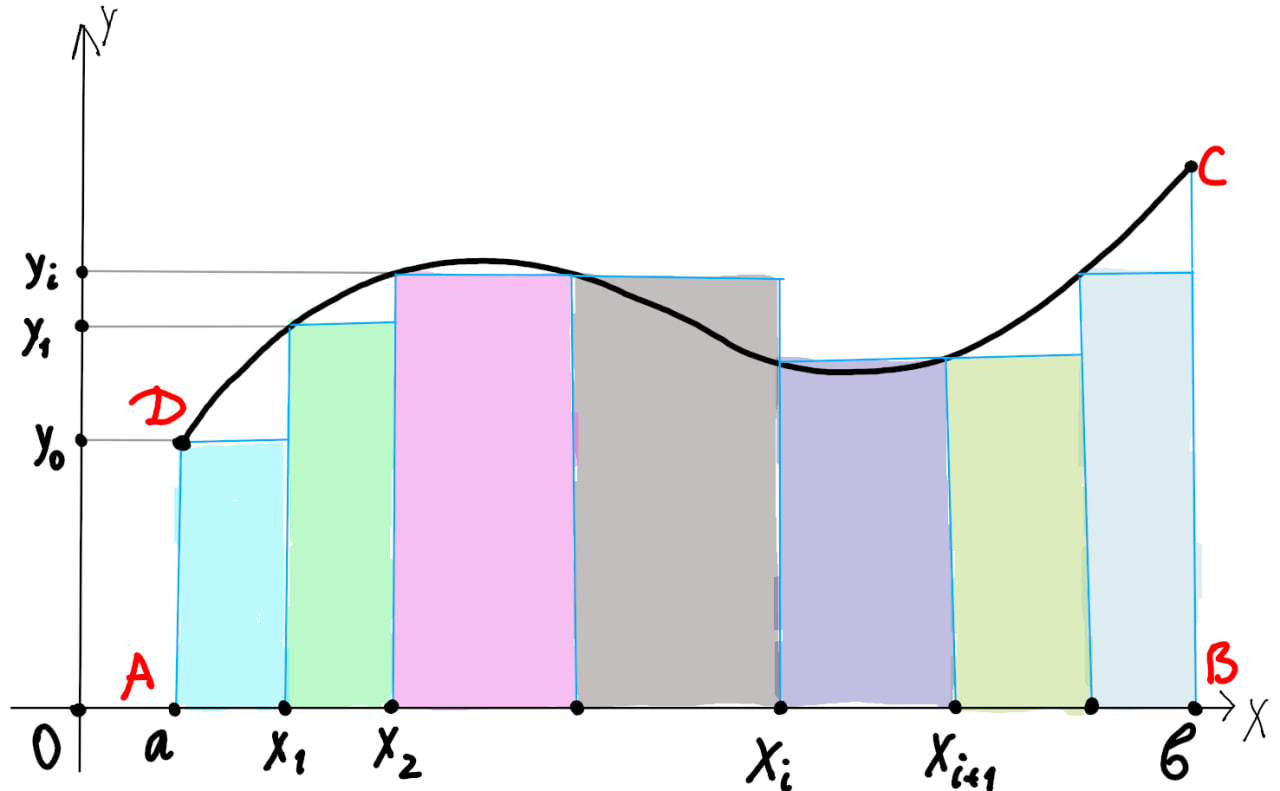
\includegraphics[scale=0.5]{int_a_b1.jpg}
    \caption{Площадь фигуры $ABCD$ примерно равна сумме площадей разноцветных прямоугольников, и чем их больше, тем точнее будет ответ.}
    \label{int_a_b}
\end{figure}

Разделим основание $AB$ нашей фигуры произвольным образом на части и проведём ординаты, соответствующие точкам деления; тогда криволинейная трапеция разобьётся на ряд полосок. 

Заменим теперь приближённо каждую полоску некоторым прямоугольником, основание которого то же, что и у полоски, а высота совпадает с одной из ординат полоски. Таким образом, криволинейная фигура заменится некоторой ступенчатой фигурой, составленной из отдельных прямоугольников. 

Обозначим абсциссы точек деления через
\[
 x_0 : = a < x_1 < x_2 < \cdots < x_i < x_{i+1} < \cdots < x_n =:b.
\]

Будем нумеровать прямоугольники числами $0,1,2,\ldots, n-1$ и пусть $S_i$ -- площадь $i$-го прямоугольника. Ясно, что $S_i = y_i \Delta x_i$, где $\Delta x_i: = x_{i+1} - x_i.$

Тогда приближённое значение площади криволинейной трапеции $S_{ABCD}$ равно
\[
 S_{ABCD} \approx \sum_{k = 0}^{n-1} y_k \Delta x_k.
\]

Тогда можно предположить, что при убывании всех $\Delta x_i$ к нулю мы будем получать более точное значение, \textit{т.е.} другими словами мы хотим сказать, что точное значение площади это следующий предел
\[
 S_{ABCD} = \lim_{\substack{\Delta x_1 \to 0 \\ \vdots \\ \Delta x_{n-1} \to 0}} \sum_{k = 0}^{n-1} y_k \Delta x_k.
\]

Для обозначения предела такой суммы вида и был Лейбницем введён символ интеграла, \textit{т.е.}
\[
 \int_a^b f(x) \mathrm{d}x : = \lim_{\substack{\Delta x_1 \to 0 \\ \vdots \\ \Delta x_{n-1} \to 0}} \sum_{k = 0}^{n-1} y_k \Delta x_k.
\]


\section{Интеграл ступенчатой функции.}

Предыдущее ``определение'' интеграла имеет очень много недостатков. Например, мы пользовались интуитивным пониманием площади криволинейной трапеции. 

Здесь мы дадим строгое определение интеграла.

\subsection{Разбиение промежутка} Напомним, что под промежутком мы понимаем подмножество прямой $\mathbb{R}$ одного из видов; $[a,b]$, $[(a,b]$, $[a,b)$, $(a,b)$, при этом мы считаем, что $|a|,|b| < \infty.$ Промежуток мы будем обозначать буквами $I$ или $J$, а под \textit{длиной промежутка} будем понимать выражение, $b-a$ и если $I$ один из рассмотренных промежутков, то будем писать $|I|: = b-a.$

\begin{mydanger}{\bf !}
    Нам также будет полезно рассматривать пустой промежуток $I$ или, если он содержит всего одну точку, то в таком случае полагаем $|I|:=0$.
\end{mydanger}

\begin{definition}
    Пусть $I$ -- промежуток, под \textit{разбиением} промежутка $I$ понимается \textbf{конечное} множество $\lambda(I)$ промежутков содержащихся в $I$, при этом любой $x \in I$ принадлежит одному и только одному промежутку из $\lambda.$
\end{definition}

\begin{example}
  Пусть $I = [1,8]$, тогда следующее множество
  \[
   \lambda(I) : = \{ \varnothing, \{1\}, (1,3), [3,5), \{5\}, (5,8]  \}
  \]
есть разбиение промежутка $I = [1,8]$, потому что любой $x \in I$ лежит в одном и только в одном из перечисленных подмножеств множества $\lambda(I)$. А если же мы положим, что
\[
 \lambda'(I): = \{ \varnothing, \{1\}, [1,3), (2,7), [3,5), \{5\}, (5,8] \}
\]
то мы уже получаем не разбиение, поскольку, например, точка $2.5 \in [1,3)$ и $2.5 \in (2,7)$.

Множество $\lambda''(I) := \{[1,4), (4,8]\}$ тоже не является разбиением промежутка $I = [1,8]$ так как $4$ не принадлежит ни одному из подмножеств множества $\lambda''(I)$. Наконец, множество $\lambda'''(I) := \{(0,5], (5,8]\}$ также не является разбиением промежутка $I = [1,8]$, потому что $(0,5]$ не содержится в $I.$
\end{example}

\begin{mydanger}{\bf !}
    Заметим, что пустое множество может не входить в разбиение промежутка. 
\end{mydanger}


\begin{theorem}[Конечная аддитивность длины]\label{additive_of_lenght}
    Пусть $I\subsetneq \mathbb{R}$ -- промежуток, а $\lambda(I)$ -- его разбиение, тогда
    \[
     |I| = \sum_{A \in \lambda(I)}|A|.
    \]
\end{theorem}
\begin{proof}
Доказывать будем по индукции, а именно по мощности разбиения. То есть для всех разбиений, в которых ровно $n$ элементов верна формула $|I| = \sum_{A \in \lambda(I)}|A|$.

(1) Если $n =0$ то значит, что $I = \varnothing$, так как любое его разбиение не должно иметь непустых элементов, но тогда формула очевидна.

(2) Если $n=1$, то это значит, что любое его разбиение имеет ровно один непустой элемент, а это значит, что $I = \{a\}$ -- одноточечное множество, но и в таком случае формула тоже очевидна.

(3) Пусть формула верна для любых разбиений, в которых ровно $n\ge 1$ элементов. И допустим теперь, что у промежутка $I$ имеются разбиения, у которых $n+1$ элементов. Именно для таких разбиений мы будем доказывать формулу. Случаи, когда $I = \varnothing$ или же когда $I = \{a\}$ очень просты для рассмотрения, так как тогда все разбиения либо содержат пустое множество, либо пустое и одноточечное.

Итак, пусть $I$ -- это одно из четырёх множеств $(a,b), (a,b], [a,b), [a,b]$.

Допустим, что $b \in I$ тогда $I$ -- это либо $(a,b]$, либо $[a,b]$. Рассмотрим произвольное разбиение $\lambda(I)$, в котором ровно $n+1$ элементов, тогда должен найтись ровно один элемент, скажем, $B$, который содержит $b$.

С другой же стороны, $B \subseteq I$, а тогда $B$ имеет либо вид $(c,b]$, либо $[c,b]$ или же $\{b\}$, где $a \le c \le b$. Для удобства можно считать, что в последнем случае $c =b$.

Рассмотрим теперь множество $I \setminus B$, которое имеет вид либо $[a,c]$, либо $(a,c)$, либо $(a,c]$, или $[a,c)$, когда $c >a$, или же $I \setminus B$ -- это точка или пустое множество. Другими словами, $I\setminus B$ -- это промежуток. 

Далее, так как $I = B \cup I \setminus B$ и $B \cap I \setminus B = \varnothing$, то множество $\lambda(I) \setminus B$ является разбиением промежутка $I\setminus B$. 

Таким образом, разбиение $\lambda(I)\setminus B$ содержит уже $n$ элементов. Но согласно предположению, для промежутка $I \setminus B$ верна формула
\[
 |I \setminus B| = \sum_{K \in \lambda(I) \setminus B} |K|
\]

Воспользовавшись теперь равенством,
\[
 |I| =|B| + |I \setminus B|
\]
мы получим

\[
 |I| = |B| + |I \setminus B| = |B| + \sum_{K \in \lambda(I) \setminus B} |K| = \sum_{A \in \lambda(I)} |A|.
\]

(4) Осталось рассмотреть случай, когда $b \notin I$, но тогда $I$ это либо $(a,b)$ либо $[a,b)$ и существует один из элементов множества $\lambda(I)$ который имеет вид либо $(c,b)$ или же $[c,b)$. Это означает, что вид множества $I \setminus B$ может принять одно из четырёх значений $[a,c]$, $(a,c)$, $(a,c]$, $[a,c)$ когда $c >a$ или же это точка или пустое множество. Остальная часть рассуждения продолжается как выше. 
\end{proof}


Эту теорему легко обобщить следующим образом.
\begin{lemma}\label{additive_of_a-lenght}
 Пусть $\alpha: I \to \mathbb{R}$ -- непрерывная функция, а $I$ -- ограниченный промежуток одного из вида $(a,b), [a,b], (a,b], [a,b)$, тогда положим
 \[
  \alpha(I): = \alpha(b) - \alpha(a).
 \]
Тогда для любого разбиения $\lambda(I)$ имеем
\[
 \alpha(I) = \sum_{A \in \lambda(I)}\alpha(A).
\]
\end{lemma}
\begin{proof}[Набросок доказательства]
    Рассуждения такие же как и в предыдущей лемме, но нужно использовать очевидное наблюдение, если $B  = [c,b] \subseteq I = [a,b]$, то $I\setminus B = [a,c)$ и тогда
    \begin{eqnarray*}
        \alpha(B) + \alpha(I \setminus B) &=& \alpha(b) - \alpha (c) + \alpha (c) + \alpha(a) \\
        &=& \alpha(b) -\alpha(a) \\
        &=& \alpha(I).
    \end{eqnarray*}
\end{proof}
 


\subsection{Ступенчатые функции}

Сейчас мы опишем класс функций, которые ``очень просты'' для интегрирования\footnote{Отметим, что эти функции также ещё называются \textit{кусочно-постоянными}, в англоязычной литературе они так и называются, \textit{piecewise constant functions.}}, а потом с помощью их мы уже определим интеграл в общем виде.  

\begin{definition}
  Пусть $A \subseteq \mathbb{R}$, и пусть дана функция $f: A \to \mathbb{R}$. Говорят, что $f$ \textit{постоянная функция}, если существует такое $\alpha \in \mathbb{R}$, что $f(x) = \alpha$ для всех $x \in A$. Если $B \subseteq A$, то говорят, что $f$ \textit{постоянная на $B$}, если существует такое $\beta \in \mathbb{R}$, что $f(y) = \beta$ для всех $y \in B.$
\end{definition}


\begin{mydanger}{\bf !}
 Из этого определения следует, что если функция $f$ постоянна на \textbf{непустом} множестве $A$, то она не может принимать два или более разных значения. Однако из определения пустого множества следует, что постоянная функция на пустом множестве может принимать \textbf{любое значение!}
\end{mydanger}

\begin{definition}
    Пусть дан промежуток $I \subsetneq \mathbb{R}$, и пусть дана функция $f: I \to \mathbb{R}$, и пусть $\lambda(I)$ -- какое-то разбиение промежутка $I$. Говорят, что \textit{функция $f$ есть ступенчатая функция на $I$ относительно $\lambda(I)$}, если для каждого $J \in \lambda(I)$, $f$ является постоянной на $J$. 
\end{definition}

\begin{example}\label{int_[1,6]=10}
    Пусть $I = [1,6]$ и определим функцию $f: [1,6]: \to \mathbb{R}$ следующим образом
    \[
     f(x) = \begin{cases}
         \,7, & 1 \le x < 3 \\
         \,4, & x = 3 \\
         \,5, & 3 < x <6 \\
         \,2, & x = 6.
     \end{cases}
    \]
Тогда, если мы рассмотрим разбиение
\[
 \lambda(I) := \Bigl\{[1,3), \{3\}, (3,6), \{6\} \Bigr\}
\]
промежутка $I$, то получаем, что $f$ -- ступенчатая функция относительно этого разбиения. Рассмотрим теперь другое разбиение этого же промежутка
\[
 \lambda'(I) : = \Bigl\{\varnothing, [1,2), \{2\}, (2,3), \{3\}, (3,5), [5,6),\{6\} \Bigr\}.
\]
Тогда несложно видеть, что $f$ будет тоже ступенчатой относительно этого разбиения. 
\end{example}

Этот пример показывает, что понятие ступенчатой функции можно определить без привлечения разбиения промежутка.

\begin{definition}\label{fiber}
Пусть $I$ -- промежуток, и пусть $\lambda(I)$, $\lambda'(I)$ -- два его разбиения. Говорят, что разбиение $\lambda'(I)$ \textit{тоньше}, чем $\lambda(I)$, если для каждого $J' \in \lambda'(I)$ найдётся такой $J \in \lambda(I)$, что $J' \subseteq J$.
\end{definition}

\begin{example}
 Вернёмся к предыдущему примеру с промежутком $I = [1,6]$ и разбиениями   
 \begin{eqnarray*}
     \lambda(I) &:=& \Bigl\{[1,3), \{3\}, (3,6), \{6\} \Bigr\},\\
     \lambda'(I) &: =& \Bigl\{\varnothing, [1,2), \{2\}, (2,3), \{3\}, (3,5), [5,6),\{6\} \Bigr\}.
 \end{eqnarray*}

Тогда видно, что $\lambda'(I)$ тоньше, чем $\lambda(I)$.
\end{example}


\begin{definition}
    Пусть дан промежуток $I \subsetneq \mathbb{R}$ и пусть дана функция $f: I \to \mathbb{R}$. Говорят, что функция $f$ \textit{ступенчатая на $I$}, если существует такое разбиение $\lambda(I)$, что $f$ -- постоянная на $I$ относительно $\lambda(I).$
\end{definition}


\begin{lemma}\label{fiber_for_functions}
  Пусть $I \subsetneq \mathbb{R}$ -- промежуток и пусть $f:I \to \mathbb{R}$ -- ступенчатая функция относительно разбиения $\lambda(I)$, тогда если имеем разбиение $\lambda'(I)$, которое тоньше, чем $\lambda(I)$, то $f$ -- ступенчатая относительно $\lambda'(I).$ 
\end{lemma}

\begin{proof}
    Действительно, пусть $A' \in \lambda'(I)$ -- произвольный элемент разбиения, тогда найдётся такой $A \in \lambda(I)$, что $A' \subseteq A$. Тогда если $f(x) = \alpha$ для всех $x \in A$, то и $f(x') = \alpha$ для всех $A'.$
\end{proof}

\begin{mydanger}{\bf !}
    Таким образом, мы будем рассматривать просто ступенчатые функции на промежутке, не определяя какое-то конкретное разбиение.
\end{mydanger}


В связи с этим уместно ввести следующее важное для дальнейшего определение.

\begin{definition}
    \textit{Характеристической функцией} некоторого множества $A \subseteq X$ называется функция $\chi_A: X\to \{0,1\}$ определённая следующим образом
    \[
     \chi_A(x): = \begin{cases}
         1 & x \in A, \\
         0 & x \notin A.
     \end{cases}
    \]
\end{definition}

\begin{remark}
 Таким образом, если $f: I \to \mathbb{R}$ -- ступенчатая функция на промежутке $I$ и пусть $\lambda(I)$ -- соответствующее разбиение промежутка $I$, тогда мы можем записать
 \[
  f =\sum_{A \in \lambda(I)} f(A) \cdot \chi_A.
 \]
\end{remark}

\begin{mydanger}{\bf !}
    Из определения следует, что $\chi_{\varnothing} = 0$, так как не существует такого $x$ чтобы $x \in \varnothing.$
\end{mydanger}


\begin{lemma}\label{chi_A+chi_B}
    Пусть $A$, $B$ два подмножества множества $X$, тогда 
    \begin{eqnarray*}
        \chi_{A \cup B} = \chi_A + \chi_B - \chi_{A\cap B},\\
        \chi_{A \cap B} = \chi_A \cdot \chi_B,\\
        \chi_{A^c} = 1 - \chi_A.
    \end{eqnarray*}
\end{lemma}

\begin{proof} (1) Пусть $x \in A\cap B$, то $x\in A$, $\chi_B$, \textit{т.е.} $\chi_A(x) = \chi_B(x) = 1$. Если $x \notin A \cup B$, то $x\notin A$, $x\notin B$ и тогда $\chi_A(x) = \chi_B(x) = 0$. В любом из этих случаев имеем $\chi_{A \cap B}(x) = \chi_A(x) \cdot \chi_B(x).$ 

(2) Пусть $x \in A^c$, тогда $x\notin A$, тогда \textit{т.е.} $\chi_{A^c}=1$, $\chi_A(x) = 0$. Если $x \notin A^c$, то $x \in A$, \textit{т.е.} $\chi_{A^c}=0$, $\chi_A(x) = 1$, что и доказывает формулу $\chi_{A^c} = 1 - \chi_A.$

(3) Наконец, так как $(A \cup B)^c = A^c \cap A^c$, то используя результаты выше, получаем
\begin{eqnarray*}
    \chi_{A \cup B} &=& 1 - \chi_{(A\cup B)^c} \\
    &=& 1 - \chi_{A^c \cap B^c} \\
    &=& 1- \chi_{A^c} \cdot \chi_{B^c} \\
    &=& 1 - (1- \chi_A)(1-\chi_B) \\
    &=& 1 - (1-\chi_B - \chi_A + \chi_{A}\cdot \chi_B) \\
    &=& 1 - 1 + \chi_A + \chi_B - \chi_{A \cap B} \\
    &=&\chi_A + \chi_B - \chi_{A \cap B}.
\end{eqnarray*}
\end{proof}


\begin{example}

Вернёмся к примеру \ref{int_[1,6]=10}, имеем $I = [1,6]$ и функцию $f: [1,6]: \to \mathbb{R}$;
    \[
     f(x) = \begin{cases}
         \,7, & 1 \le x < 3 \\
         \,4, & x = 3 \\
         \,5, & 3 < x <6 \\
         \,2, & x = 6.
     \end{cases}
    \]
Как мы уже видели, $f$ -- ступенчатая относительно разбиений
\begin{align*}
    &  \lambda(I) := \Bigl\{[1,3), \{3\}, (3,6), \{6\} \Bigr\},\\
    &  \lambda'(I) : = \Bigl\{\varnothing, [1,2), \{2\}, (2,3), \{3\}, (3,5), [5,6),\{6\} \Bigr\}.
\end{align*}

Тогда получаем, что
\[
 f = 7 \cdot \chi_{[1,3)} + 4 \cdot \chi_{\{3\}} + 5 \cdot \chi_{(3,6)} + 2 \cdot \chi_{\{6\}},  
\]
а также
\[
f = \alpha \cdot \chi_{\varnothing} + 7 \cdot \chi_{[1,2)} + 7 \cdot \chi_{\{2\}} + 7 \cdot \chi_{(2,3)} + 4 \cdot \chi_{\{3\}} + 5 \cdot \chi_{(3,5)} + 5 \cdot \chi_{[5,6)} + 2 \cdot \chi_{\{6\}},
\]
где $\alpha \in \mathbb{R}$ -- произвольное число, но так как $\chi_\varnothing = 0$, то всё корректно.
\end{example}

\begin{proposition}\label{beautefull}
    Пусть имеем две ступенчатые функции $f,g:I \to \mathbb{R}$ и пусть $\lambda_f(I) = \cup_{p=1}^n A_p$, $\lambda_g(I) = \cup_{q=1}^m B_q$ -- разбиения промежутка $I$ такие, что $f$, $g$ -- ступенчаты относительно $\lambda_f(I)$ и $\lambda_g(I)$ соответственно. Тогда $\lambda(I): = \cup_{p=1}^n \cup_{q=1}^m A_p \cap B_q$ -- разбиение промежутка $I$, и более того каждая из функций $f,g$ ступенчата относительно него и
    \begin{align*}
        & f =  \sum_{p=1}^n\sum_{q=1}^m f(A_p) \cdot \chi_{A_p}\cdot \chi_{B_q}\\
        & g=  \sum_{p=1}^n\sum_{q=1}^m g(B_q) \cdot \chi_{A_p} \cdot \chi_{B_q}.
    \end{align*}
\end{proposition}

\begin{proof} Покажем, что это разбиение. Так как $I = \cup_{p=1}^n A_p = \cup_{q= 1}B_q$, то
\[
 \cup_{p=1}^n \cup_{q=1}^m A_p \cap B_q  = \left( \cup_{p=1}^n A \right) \cap \left( \cup_{q=1}^m B_q \right) = I \cap I = I,
\]
в силу того, что $A_p \cap A_{p'} = \varnothing$ и $B_q \cap B_{q'} = \varnothing$, то $(A_p \cap B_q) \cap (A_{p'}\cap B_{q'}) = \varnothing$, $1\le p \le n$, $1\le q \le m$. Поэтому $\lambda(I)$ -- разбиение промежутка $I$.


Далее, так как $\lambda_f(I)$, $\lambda_g(I)$ разбиения, то для любых $1\le p \le n$, $1\le q \le m$, имеем
\[
 A_p = \cup_{q=1}^m (A_p \cap B_q), \qquad B_q = \cup_{p=1}^n (A_p \cap B_q).
\]

Наконец, так как $\chi_\varnothing = \varnothing$, и пользуясь леммой \ref{chi_A+chi_B}, получаем
\begin{eqnarray*}
    f &=& \sum_{p=1}^n f(A_p) \cdot \chi_{A_p} \\
    &=& \sum_{p=1}^n\sum_{q=1}^m f(A_p) \cdot \chi_{ \cup_{q=1}^m (A_p \cap B_q)} \\
    &=& \sum_{q=1}^m f(A_p) \cdot \left(\chi_{A_p \cap B_1} + \cdots + \chi_{A_p \cap B_m} \right) \\
    &=& \sum_{p=1}^n\sum_{q=1}^m f(A_p) \cdot \chi_{A_p \cap B_q}.
\end{eqnarray*}

Аналогично доказывается формула для функции $g.$
    
\end{proof}


\begin{corollary}\label{cor_for_sum}
 Пусть $I \subsetneq \mathbb{R}$ -- промежуток и пусть $f,g:I \to \mathbb{R}$ -- ступенчатые функции на нём. Тогда функции
    \[
     f\pm g, \quad \max\{f,g\}, \quad f\cdot g
    \]
    тоже ступенчатые на $I$. Если $g(x) \ne 0$ при $x \in I$, то $\frac{f}{g}$ тоже ступенчатая функция на $I.$    
\end{corollary}
    

\begin{proof}

Пусть $\lambda_f(I)  =  \cup_{p=1}^n A_p$, $\lambda_g(I) =  \cup_{q=1}^m B_q$ -- разбиения промежутка $I$ относительно которых $f$, $g$ -- ступенчаты, соответственно. Согласно предложению \ref{beautefull},
  \begin{align*}
        & f =  \sum_{p=1}^n\sum_{q=1}^m f(A_p) \cdot \chi_{A_p}\cdot \chi_{B_q}\\
        & g=  \sum_{p=1}^n\sum_{q=1}^m g(B_q) \cdot \chi_{A_p} \cdot \chi_{B_q}.
    \end{align*}

Тогда, получаем
\begin{eqnarray*}
    f \pm g &=& \sum_{p=1}^n\sum_{q=1}^m (f(A_p) \pm g(B)q) \cdot \chi_{A_p}\cdot \chi_{B_q} \\
     \max\{f ,g\} &=& \sum_{p=1}^n\sum_{q=1}^m \max\{f(A_p), g(B)q)\} \cdot \chi_{A_p}\cdot \chi_{B_q},\\
      f \cdot g &=& \sum_{p=1}^n\sum_{q=1}^m (f(A_p) \cdot g(B)q) \cdot \chi_{A_p}\cdot \chi_{B_q},\\
     \frac{f}{ g} &=& \sum_{p=1}^n\sum_{q=1}^m \left(\frac{f(A_p)}{ g(B_q)}\right) \cdot \chi_{A_p}\cdot \chi_{B_q},\qquad g \ne 0,
\end{eqnarray*}
что и требовалось доказать.
\end{proof}

\subsection{Интеграл от ступенчатой функции на промежутке}

Итак, у нас всё готово, чтобы ввести следующее важное определение.

\begin{definition}\label{int_of_p.c_on_I}
    Пусть $I \subsetneq \mathbb{R}$ -- промежуток, $\lambda(I)$ -- разбиение промежутка $I$ и пусть $f:I \to \mathbb{R}$ -- ступенчатая функция относительно этого разбиения, \textit{т.е.} $f = \sum_{A \in \lambda(I)}f(A) \cdot \chi_A$. Определим \textit{интеграл на промежутке $I$} ступенчатой функции $f:I \to \mathbb{R}$ относительно разбиения $\lambda(I)$ следующим образом
    \[
     \int_{\lambda(I)}f: =  \sum_{A \in \lambda(I)} f(A)\cdot |A|
    \]
\end{definition}

\begin{mydanger}{\bf !}
     Во-первых, что стоит слева от равно нужно понимать как символ и не более того! Во-вторых, это определение может показаться некорректным если $\lambda(I)$ содержит пустое множество, но так как $|\varnothing| = 0$, то мы на самом деле получаем корректное определение.     
\end{mydanger}

\begin{remark}\label{int_via_chi}
    Если $f = \chi_I$, и взяв разбиение $\lambda(I) = \{I\}$ то мы получаем следующее
    \[
     \int_{\lambda(I)}\chi_I = |I|.
    \]
И тогда мы можем записать, что если $f = \sum_{A \in \lambda(I)}f(A) \cdot \chi_A$, то
\[
\boxed{
 \int_{\lambda(I)}f = \sum_{A \in \lambda(I)} f(A) \cdot \int_{\lambda(I)}\chi_A
 }
\]
\end{remark}


\begin{example}\label{int_[1,4]=10}
    Пусть $f: [1,4] \to \mathbb{R}$ определена следующим образом
    \[
     f(x)  = \begin{cases}
          \, 2 & 1 \le x <3 \\
          \, 4 & x = 3 \\
          \, 6 & 3< x \le 4
     \end{cases}
    \]
    и пусть $\lambda(I) = \{ [1,3), \{3\}, (3,4] \}$, тогда
 \begin{eqnarray*}
  \int_{\lambda(I)} f  &=& \alpha_{[1,3)}\cdot | [1,3) | + \alpha_{\{3\}}\cdot |\{3\}| + \alpha_{(3,4]} \cdot | (3,4] | \\
  &=& 2 \cdot 2 + 4 \cdot 0 + 6 \cdot 1 \\
  &=& 10.
 \end{eqnarray*}

 С другой стороны, рассмотрим такое разбиение $\lambda'(I) = \{ \varnothing, [1,2), [2,3), \{3\}, (3,4] \}$, нетрудно видеть, что оно тоньше разбиения $\lambda(I)$. Находим
 \begin{eqnarray*}
     \int_{\lambda'(I)}f &=&\alpha_\varnothing \cdot |\varnothing| + \alpha_{[1,2)} \cdot | [1,2) | + \alpha_{[2,3)} \cdot |[2,3)| + \alpha_{\{3\}}\cdot |\{3\}| + \alpha_{(3,4]} \cdot | (3,4] | \\
     &=& \alpha_\varnothing \cdot 0 + 2 \cdot 1 + 2 \cdot 1 + 4 \cdot 0 + 6 \cdot 1 \\
     &=& 10.
 \end{eqnarray*}
 
\end{example}

Итак, мы увидели, что, взяв разбиение тоньше, значение интеграла не изменилось, очевидно, что это верно и в общем случае.

\begin{lemma}
  Пусть $I \subsetneq \mathbb{R}$ -- промежуток и пусть $f:I \to \mathbb{R}$ -- ступенчатая функция относительно разбиения $\lambda(I)$, тогда если имеем разбиение $\lambda'(I)$, которое тоньше, чем $\lambda(I)$, то
  \[
   \int_{\lambda(I)}f = \int_{\lambda'(I)}f.
  \]
\end{lemma}

\begin{proof}
    Пусть $\lambda(I) = \{ A_1,\ldots, A_n \}$ и пусть 
    \[
     \lambda'(I) : = \Bigl\{A_{11}', \ldots, A'_{1\ell_1},\ldots, A'_{n1},\ldots, A'_{n\ell_n} \Bigr\},
    \]
    где $A_i$ содержит только $A'_{i1},\ldots, A'_{i\ell_i}$, $1\le i \le n$. Из определения \ref{fiber} тогда следует, что $A_i = A'_{i1} \cup \cdots \cup A'_{i\ell_i}$ и $|A_i| = |A'_{i1}| + \cdots + |A'_{i\ell_i}|$.
    
    Наконец, используя лемму \ref{fiber_for_functions}, получаем, что
    \[
     f(A'_{i1}) = \cdots = f(A'_{i\ell_i}) = f(A_i), \qquad 1 \le i \le \ell.
    \]

    Таким образом, имеем
    \begin{eqnarray*}
        \int_{\lambda'(I)}f &=& \Bigl(f(A_{11}') \cdot \left| A'_{11} \right| + \cdots + f(A_{1\ell_1})\cdot \left|A'_{i\ell_1}\right|\Bigr) + \cdots + \Bigl(f(A_{11}') \left|A_{11}'\right| + \cdots + f(A_{1\ell_1})\cdot \left|A'_{i\ell_1}\right| \Bigr) \\
        &=& f(A_1) \cdot \left( \left| A'_{11}  \right| + \cdots + \left| A'_{1\ell_1} \right| \right) + \cdots + f(A_n) \cdot \left( \left| A'_{n1}  \right| + \cdots + \left| A'_{n\ell_n} \right| \right) \\
        &=& f(A_1) |A_1| + \cdots + f(A_n)\cdot |A_n| \\
        &=& \int_{\lambda(I)}f.
    \end{eqnarray*}
\end{proof}


Таким образом, мы можем ввести следующее определение, которое будем использовать в дальнейшем.

\begin{definition}\label{int_of_p.c}
    Пусть $I \subsetneq \mathbb{R}$ -- промежуток, $f:I \to \mathbb{R}$ -- ступенчатая функция на нём. Определим \textit{интеграл на промежутке $I$} ступенчатой функции $f:I \to \mathbb{R}$ следующим образом
    \[
     \int_If: =  \int_{\lambda(I)}f,
    \]
    где $\lambda(I)$ такое разбиение промежутка $I$, что $f$ является ступенчатой относительно $\lambda(I).$
\end{definition}


\begin{example}
Вернёмся к примеру \ref{int_[1,4]=10}. Пусть $f: [1,4] \to \mathbb{R}$ определена следующим образом
    \[
     f(x)  = \begin{cases}
          \, 2 & 1 \le x <3 \\
          \, 4 & x = 3 \\
          \, 6 & 3< x \le 4
     \end{cases}
    \]
    и пусть $\lambda(I) = \{ [1,3), \{3\}, (3,4] \}$, тогда
 \begin{eqnarray*}
  \int_{\lambda(I)} f  &=& \alpha_{[1,3)}\cdot | [1,3) | + \alpha_{\{3\}}\cdot |\{3\}| + \alpha_{(3,4]} \cdot | (3,4] | \\
  &=& 2 \cdot 2 + 4 \cdot 0 + 6 \cdot 1 \\
  &=& 10.
   \end{eqnarray*}

Тогда
\[
 \int_{[1,4]}f   =10.
\]
\end{example}

\begin{theorem}\label{imprtant_for_int}
    Пусть $I \subsetneq \mathbb{R}$ -- промежуток и $f,g:I \to \mathbb{R}$ -- две ступенчатые функции на нём.
    \begin{enumerate}
        \item \[
        \int_I( f \pm  g) =  \int_I f  \pm  \int_I g , \qquad \alpha, \beta \in \mathbb{R}.
        \]
        \item Если $f(x) \ge g(x)$ для всех $x \in I$, то
        \[
         \int_I f \ge \int_I g.
        \]

        \item Если $f(x) = \alpha$ для всех $x \in I$, то
        \[
         \int_I f = \alpha \cdot |I|.
        \]
        \item Если $I \subseteq J$ и если $\varphi: J \to \mathbb{R}$ функция, определённая следующим образом
        \[
         \varphi(x) : = \begin{cases}
             f(x) & x \in I,\\
             0 & x \notin I,
         \end{cases}
                 \]
    тогда $\varphi(x)$ -- ступенчатая на $J$ и 
    $$\int_J\varphi   = \int_I f.$$
    
    \item Пусть $\{A,B\}$ -- разбиение промежутка $I$, тогда если функции $f|_A:A \to \mathbb{R}$, $f|_B:B \to \mathbb{R}$ ступенчаты на $A$ и $B$ соответственно, то
    \[
     \int_I f  = \int_A f|_A  + \int_B f|_B .
    \]

    \end{enumerate}
\end{theorem}

\begin{proof}

Пусть $\lambda_f(I)  =  \cup_{p=1}^n A_p$, $\lambda_g(I) =  \cup_{q=1}^m B_q$ -- разбиения промежутка $I$ относительно которых $f$, $g$ -- ступенчаты, соответственно. Согласно предложению \ref{beautefull},
  \begin{align*}
        & f =  \sum_{p=1}^n\sum_{q=1}^m f(A_p) \cdot \chi_{A_p}\cdot \chi_{B_q} = \sum_{p=1}^n\sum_{q=1}^m f(A_p) \cdot \chi_{A_p\cap B_q}, \\
        & g=  \sum_{p=1}^n\sum_{q=1}^m g(B_q) \cdot \chi_{A_p} \cdot \chi_{B_q} = \sum_{p=1}^n\sum_{q=1}^m g(B_q) \cdot \chi_{A_p\cap B_q}.
    \end{align*}

(1) Согласно следствию \ref{cor_for_sum}, $f\pm g = \sum_{p=1}^n\sum_{q=1}^m (f(A_p) \pm g(B_q)) \cdot \chi_{A_p\cap B_q}$, и тогда пользуясь замечанием \ref{int_via_chi},
\begin{eqnarray*}
    \int_I (f\pm g) &=& \sum_{p=1}^n\sum_{q=1}^m (f(A_p) \pm g(B_q)) \cdot \int_I \chi_{A_p \cap B_q} \\
    &=&\sum_{p=1}^n\sum_{q=1}^m f(A_p) \cdot \int_I \chi_{A_p \cap B_q} \pm \sum_{p=1}^n\sum_{q=1}^m g(B_q) \cdot \int_I \chi_{A_p \cap B_q} \\
    &=& \int_I f \pm \int_I g.
\end{eqnarray*}

(2) Если $f(x) \ge g(x)$ для всех $x\in I$, то для любых $p,q$ таких, что $A_p \cap B_q \ne \varnothing$, имеем $f(A_p) \ge g(B_q)$. Тогда, согласно замечанию \ref{int_via_chi},
\begin{eqnarray*}
    \int_I f &:=&  \sum_{p=1}^n\sum_{q=1}^m f(A_p) \cdot \int_I \chi_{A_p \cap B_q} = \sum_{p=1}^n\sum_{q=1}^m f(A_p) \cdot |A_p \cap B_q| \\
    &\ge & \sum_{p=1}^n\sum_{q=1}^m g(A_p) \cdot |A_p \cap B_q| \\
    &=& \sum_{p=1}^n\sum_{q=1}^m f(A_p) \cdot \int \chi_{A_p \cap B_q} \\
    &=:& \int_I g.
\end{eqnarray*}

(3) Если $f(x) = \alpha$ для всех $x\in I$, то $f = \alpha \cdot \chi_I$, и согласно замечанию \ref{int_via_chi},
\[
 \int_f f = \alpha\cdot \int \chi_I = \alpha \cdot |I|.
\]

(4) Пусть $\lambda(I)$ -- разбиение промежутка $I$ и $f = \sum_{A \in \lambda(I)} f(A) \cdot \chi_A$, то определим разбиение $\lambda(J)$ промежутка $J$ следующим образом
\[
 \lambda(J): = \lambda(I) \cup \{J\setminus I\}
\]
положим, что $\varphi(J\setminus I) :=0$ мы получаем, что $\varphi$ -- ступенчата на $J.$ Мы можем также записать
\[
 \varphi = \sum_{A \in \lambda(I)} f(A) \chi_A + \varphi(J\setminus I) \chi_{J \setminus I}
\]
тогда согласно Замечанию \ref{int_via_chi},
\begin{eqnarray*}
  \int_J \varphi &=& \sum_{A \in \lambda(I)} f(A) \int_J \chi_A + \varphi(J\setminus I) \int_J \chi_{J \setminus I}   \\
 &=& \sum_{A \in \lambda(I)} f(A) \cdot |A| + 0 \cdot |J \setminus I|\\
 &=& \int_I f.
\end{eqnarray*}

(5) Пусть $\lambda(A): = \cup_{p=1}^n A_p$, $\lambda(B) : = \cup_{q=1}^m B_q$ -- разбиения промежутков $A,B$ соответственно. Тогда $\lambda : = \lambda(A) \cup \lambda(B)$ разбиение промежутка $I.$ 

Имеем
\[
  f = \sum_{C \in \lambda(I)} f(C) \cdot \chi_C = \sum_{p=1}^n f(A_p)\cdot \chi_{A_p} + \sum_{q=1}^m f(B_q)\cdot \chi_{B_q} = f|_A + f|_B,
\]
тогда согласно замечанию \ref{int_via_chi},
\begin{eqnarray*}
  \int_I f &=& \sum_{C \in \lambda(I)} f(C) \cdot \int_I \chi_C \\
  &=& \sum_{C \in \lambda(I)} f(C) \cdot |C| \\
  &=& \sum_{p=1}^n f(A_p) \cdot |A_p| + \sum_{q=1}^m f(B_q)\cdot |B_q| \\
  &=& \int_A f|_A + \int_B f|_B.
\end{eqnarray*}
\end{proof}



\section{Интеграл от ограниченной функции на промежутке}

Пусть теперь $f:I \to \mathbb{R}$ будет ограниченной функцией на промежутке $I\subsetneq \mathbb{R}$. Мы хотим распространить на такой класс функций понятие интеграла. Чтобы это сделать, мы обратимся к ограниченным последовательностям. Мы знаем (см. Теорема \ref{from_bounded_sequence}), что у любой ограниченной последовательности имеется верхний и нижний пределы ($\lim \sup$, $\lim \inf$ соответственно.) 

С определением интеграла для ограниченной функции на промежутке мы будем поступать аналогичным образом. Позже мы объясним почему нужны именно ограниченные функции.

\begin{definition}
    Пусть $f,g: I \to \mathbb{R}$ -- две функции, мы говорим, что $g$ \textit{мажорирует} $f$ на $I$, если $g(x) \ge f(x)$ для всех $x \in I$ или же мы говорим, что $f$ \textit{минорирует} $g$ на $I.$ Множество всех функций которые мажорируют $f$ на промежутке $I$ обозначим через $M(f)$, множество всех функций которые минорируют $f$ на промежутке $I$ обозначим через $m(f).$
\end{definition}


\subsection{Верхний и нижний интегралы}

Введём теперь понятия верхнего и нижнего интеграла по аналогии с верхним и нижним пределами последовательности.

\begin{definition}\label{Riemann_int}
 Пусть $f: I \to \mathbb{R}$ -- ограниченная функция на промежутке $I \subsetneq \mathbb{R}$. Определим \textit{верхний интеграл функции $f$ на промежутке $I$} следующим образом
 \[
      \overline{ \int_I} f  : = \inf  \left\{ \int_I g  , \, g \in M_{p.c}(f)\right\},
 \]
 а \textit{нижний интеграл функции $f$ на промежутке $I$} мы определим следующим образом
 \[
  \inf \int_I f  : = \sup  \left\{ \int_I g  , \, g \in m_{p.c}(f) \right\}.
 \]
\end{definition}

\begin{lemma}\label{inf_int<sup_int}
    Пусть $f:I \to \mathbb{R}$ -- ограниченная функция на промежутке $I \subsetneq \mathbb{R}$, числами $a,b$,\textit{т.е.} $a \le f(x) \le b$ для всех $x \in I$. Тогда
    \[
     a\cdot |I| \le \inf \int_I f  \le \overline{\int_I} f \le b \cdot |I|.
    \]
\end{lemma}
\begin{proof}
    Рассмотрим функции $a,b:I \to \mathbb{R}$, $a(x) := a$, $b(x): =b$, $x\in I$. Тогда $a \in m(f)$, $b \in M(f)$, тогда по определению $\sup, \inf$ (см. Определение \ref{sup,inf}), получаем
    \[
     \overline{\int_I} f\le \int_I b = b \cdot |I|, \qquad \inf \int_I f \ge \int_I a = a\cdot |I|.
    \]

Покажем теперь, что 
    $$\inf \int_I f \le \overline{\int_I} f.$$
    
Пусть $h\in m(f)$, $g\in M(f)$, и они -- ступенчатые функции, тогда $h \le g$ и по теореме \ref{imprtant_for_int} (2), получаем 
$$
\int_I h \le \int_I g.
$$

Отсюда вытекает
    \[
     \inf \int_I f :=\sup \left\{ \int_I h, \, h \le g \right\} \le \inf \left\{ \int_I g,\, g \ge h\right\} =: \overline{\int_I}f,
    \]
    что и требовалось доказать.
\end{proof}

\begin{corollary}
 Верхний и нижний интеграл от ограниченной функции всегда существует.
\end{corollary}

\begin{proof} Пусть $f:I \to \mathbb{R}$ -- ограниченная функция, скажем $a\le f(x) \le b$, $x \in I$, на ограниченном промежутке $I \subsetneq \mathbb{R}$. По только что доказанной лемме (см. Лемма \ref{inf_int<sup_int}), имеем
\[
 \inf \int_I f, \,\overline{\int_I}f \in [A,B], \qquad A: = a \cdot |I|, \, B:=b\cdot |I|,
\]
что и доказывает утверждение.
\end{proof}



Таким образом, следующее определение корректно.

\begin{definition}[{Интеграл Римана от ограниченной функции}]\label{int_of_bounded} Пусть $f:I \to \mathbb{R}$ -- ограниченная функция на ограниченном промежутке $I \subsetneq \mathbb{R}$, тогда если
\[
 \inf \int_I f = \overline{\int_I} f
\]
то мы определим \textit{интеграл Римана от ограниченной функции $f$} следующим образом
\[
 \int_I f: = \inf \int_I f = \overline{\int_I}f .
\]
\end{definition}

\begin{remark}\label{why_bounded}
 Теперь ясно, почему мы рассматриваем только ограниченные функции на ограниченном промежутке. Ведь в противном случае верхний или нижний интегралы просто могут не существовать.    
\end{remark}



\begin{lemma}\label{int_coinside}
    Пусть $f: I \to \mathbb{R}$ -- ступенчатая функция на ограниченном промежутке $I \subsetneq \mathbb{R}$, тогда она интегрируема по Риману, и более того интеграл Римана от неё это то же самое, что и интеграл от ступенчатой функции (см. определение \ref{int_of_p.c}).
\end{lemma}

\begin{proof}
Так как $f$ -- ступенчата и $f(x) \le f(x)$ для всех $x \in I$, то $f\in M_{p.c}(f)$, $f \in m_{p.c.}(f)$, а тогда 
\[
 \overline{\int_I} f \le \int_I f, \qquad \inf \int_I f \ge \int_I f,
\]
\textit{т.е.}
\[
 \overline{\int_I} f \le \int_I f \le \inf \int_I f,
\]
но согласно лемме \ref{inf_int<sup_int}, 
\[
 \inf \int_I f \le \overline{\int_I} f
\]
откуда получаем, что
\[
 \inf \int_I f = \overline{\int_I} f,
\]
что и доказывает утверждение.
\end{proof}


Другими словами, для ступенчатой функции, определение интеграла которое мы дали для произвольных ограниченных функций совпадает с определением интеграла от ступенчатой функции. Таки образом, мы расширили определение интеграла \ref{int_of_p.c} на более широкий класс функций.

\subsection{Верхние и нижние суммы Римана}

Здесь мы докажем важные свойства интеграла от ограниченной функции.

\begin{definition}\label{up_and_low_Riman}
    Пусть $f:I \to \mathbb{R}$ -- ограниченная функция на ограниченном промежутке $I \subsetneq \mathbb{R}$ и пусть $\lambda(I)$ -- некоторое разбиение промежутка $I$. Определим \textit{верхнюю и нижнюю суммы Римана} следующим образом
    \[
 {U}(f, \lambda(I)): = \sum_{\substack{A \in \lambda(I) \\ A \ne  \varnothing}} \sup_{x\in A} f(x)\cdot |A|
     \]
     и
     \[
      {L}(f, \lambda(I)): = \sum_{\substack{A \in \lambda(I) \\ A \ne  \varnothing}} \inf_{x\in A} f(x)\cdot |A|
     \]
\end{definition}

\begin{mydanger}{\bf !}
    Условие, что $A \ne \varnothing$ здесь очень существенно, ведь если $A = \varnothing$, то $f(x)$ -- это \textbf{любое число}, и тогда $\sup_{x\in \varnothing} f(x), \sup_{x\in \varnothing} f(x)= \pm \infty.$
\end{mydanger}

\begin{remark}\label{U=int}
    Для данной ограниченной функции $f:I \to \mathbb{R}$ и для данного разбиения $\lambda: = \lambda(I)$ мы рассмотрим функции $\overline{f_\lambda}, \underline{f_\lambda}: I\to \mathbb{R}$, определённые следующим образом
    \[
     \overline{f_\lambda}(x): = \sup_{x\in A, A \in \lambda(I)} f(x),\qquad \underline{f_\lambda}(x): = \inf_{x\in A, A \in \lambda(I)} f(x).
    \]

Из этой конструкции следует, что $\overline{f_\lambda} \in M_{p.c}(f,\lambda(I))$ и $\underline{f_\lambda} \in m_{p.c}(f,\lambda(I)).$ Тогда воспользовавшись определениями \ref{int_of_p.c_on_I}, \ref{int_of_p.c}, можно записать
    \[
     U(f,\lambda(I)) = \int_I \overline{f_\lambda}, \qquad L(f,\lambda(I)) = \int_I \underline{f_\lambda}.
    \]
\end{remark}



\begin{lemma}\label{intg>U}
Пусть $f: I \to \mathbb{R}$ -- ограниченная функция на ограниченном промежутке $I \subsetneq \mathbb{R}$ и пусть $g,h$ -- ступенчатые функции на $I$ и $g \in M(f), h \in m(f)$, тогда
\[
 \int_I g \ge U(f, \lambda_g(I)), \qquad \int_I h \le L(f, \lambda_h(I)),
\]
где $\lambda_g(I)$, $\lambda_h(I)$ -- разбиения промежутка $I$ относительно которых $g,h$ ступенчаты, соответственно.
\end{lemma}

\begin{proof}
    Согласно определениям \ref{int_of_p.c_on_I}, \ref{int_of_p.c} имеем
    \begin{eqnarray*}
        \int_I g &: =& \int_{\lambda_g(I)}g = \sum_{A \in \lambda_g(I)}g(A)\cdot |A|,\\
        \int_I h &: =& \int_{\lambda_h(I)}h = \sum_{B \in \lambda_h(I)}h(B)\cdot |B|,
    \end{eqnarray*}
а так как $g \in M(f)$, $h\in m(f)$, то для всех $A \in \lambda_g(I)$, $B \in \lambda_h(I)$ имеем $g(A) \ge f(x)$, $h(B)\le f(y)$, $x \in A$, $y \in B$ но тогда
\begin{eqnarray*}
    \int_I g &: =& \int_{\lambda_g(I)}g = \sum_{A \in \lambda_g(I)}g(A)\cdot |A| \ge \sum_{\substack{A \in \lambda_f(I) \\ A \ne  \varnothing}} \sup_{x\in A} f(x)\cdot |A| =: U(f, \lambda_g(I)),\\
    \int_I h &: =& \int_{\lambda_h(I)}h = \sum_{B \in \lambda_h(I)}h(B)\cdot |b| \le \sum_{\substack{B \in \lambda_h(I) \\ B \ne  \varnothing}} \inf_{y\in B} f(y)\cdot |B| =: L(f, \lambda_g(I)),
\end{eqnarray*}
что и требовалось доказать.
\end{proof}



\begin{corollary}\label{cor_for_supint}
    Пусть $f:I \to \mathbb{R}$ -- ограниченная функция на ограниченном промежутке $I$, тогда
    \[
     \overline{\int_I} f = \inf \Bigl\{ U(f, \lambda(I))\, : \, \mbox{$\lambda(I) $-- разбиение промежутка $I$} \Bigr\}
    \]
    и
    \[
     \inf \int_I f = \sup \Bigl\{ L(f, \lambda(I))\, : \, \mbox{$\lambda(I) $-- разбиение промежутка $I$} \Bigr\}.
    \]   
\end{corollary}
 
\begin{proof} Мы докажем первое утверждение, так как второе доказывается аналогично.

Пусть $\lambda(I)$ --произволбное разбиение промежутка $I$, тогда рассмотрим множество $M_{p.c}(f, \lambda(I))$ всех ступенчатых относительно разбиения $\lambda(I)$ функции которые мажорируют функцию $f$ (\textit{соотв.} минорируют функцию f).

(1) Покажем, что 
\[
 \overline{\int_I} f \ge \inf_{\lambda(I)} \{U(f, \lambda(I))\}.
\]

Для любой $g\in M(f, \lambda(I))$, по лемме \ref{intg>U}, 
 \[
   U(f, \lambda(I)) \le \int_I g,
 \]
тогда используя определение инфинума, имеем
\[
 \int_I g \ge U(f,\lambda(I)) \ge \inf\{U(f,\lambda(I))\}
\]
для любой $g\in M(f, \lambda(I))$. Так как это неравенство верно для любого разбиения $\lambda(I)$, то получаем
\[
\overline{\int_I} f: = \inf \left\{ \int_I g\, :\, g \in M_{p.c}(f) \right\} \ge \inf\{U(f,\lambda(I))\},
\]
а это мы и хотели показать.

(2) Покажем, что

\[
 \overline{\int_I} f \le \inf_{\lambda(I)} \{U(f, \lambda(I))\}.
\]

Согласно определению \ref{Riemann_int},
\[
\sup\int_I f : = \inf  \left\{ \int_I g  , \, g \in M_{p.c}(f)\right\} \le \int_I \overline{f_\lambda} = U(f,\lambda(I)),
\]
здесь мы воспользовались замечанием \ref{U=int}. Это завершает доказательство.
\end{proof}

\subsection{Основные свойства интеграла}

Здесь мы покажем основные свойства интеграла, которые будут необходимы нам для дальнейшего.

\begin{theorem}\label{mega_theorem_for_int}
    Пусть $I \subsetneq \mathbb{R}$ -- ограниченный промежуток и пусть $f,g: I \to \mathbb{R}$ -- ограниченные функции на нём и при этом они интегрируемы на нём по Риману.

    \begin{enumerate}
        \item Функция $f+g$ интегрируема на $I$ и более того
        \[
         \int_I (f+g) = \int_I f + \int_I g.
        \]
        \item Для любого $\alpha \in \mathbb{R}$, функция $\alpha\cdot f$ -- интегрируема на $I$ и более того
        \[
         \int_I \alpha\cdot f = \alpha \cdot \int_I f.
        \]
        \item Функция $f-g$ интегрируема на $I$ и более того
        \[
         \int_I(f-g)  = \int_I f - \int_I g.
        \]
        \item Если $f(x) \ge 0$ для всех $x\in I$, то
        \[
         \int_I f \ge 0.
        \]
        \item Если $f(x) \ge g(x)$ для всех $x \in I$, то
        \[
         \int_I f \ge \int_I g.
        \]
        \item Если $f(x) = \alpha$ для всех $x \in I$, то
        \[
         \int_I f = \alpha\cdot |I|.
        \]
        \item Пусть $J \subsetneq \mathbb{R}$ -- ограниченный промежуток, и $I \subseteq J$ и пусть $\varphi:J \to \mathbb{R}$ -- функция определённая следующим образом
        \[
         \varphi(x): = \begin{cases}
             f(x), & x\in I,\\
             0, & x \notin I.
         \end{cases}
        \]
        Тогда $\varphi$ -- интегрируема на $J$ и более того
        \[
         \int_J \varphi = \int_I f.
        \]
        \item Пусть $\{A,B\}$ -- разбиение $I$, тогда функции $f|_A$, $f|_B$ -- интегрируемы на $A$, $B$ соответственно и более того
        \[
         \int_I f = \int_A f|_A + \int_B f|_B.
        \]
    \end{enumerate}
\end{theorem}
\begin{proof}

Пусть $\overline{f}$ (\textit{соотв.} $\underline{f}$) -- функция из $M_{p.c}(f)$ (\textit{соотв.} из $m_{p.c}(f)$). Тогда, ясно, что $\overline{f}+\overline{g} \in M_{p.c}(f+g)$ и $\underline{f}+ \underline{g} \in m_{p.c}(f+g).$

Если $f$ -- интегрируема по Риману на $I$, то, согласно определению \ref{int_of_bounded}
\[
 \int_I f = \overline{\int_I} f = \inf \int_I f.
\]

Тогда по определению $\inf$, $\sup$ для любого $\varepsilon >0$ найдутся такие $\overline{f} \in M_{p.c}(f)$, $\underline{f} \in m_{p.c}(f)$ что
\begin{equation}\label{non_for_Th}
  \int_I f + \varepsilon = \overline{\int_I} f+ \varepsilon > \int_I \overline{f}, \qquad \int_I f - \varepsilon = \inf \int_I f - \varepsilon < \int_I \underline{f}.    
\end{equation}


(1) Покажем, что $f+g$ интегрируема по Риману. Воспользуемся определением \ref{int_of_bounded}, Теоремой \ref{imprtant_for_int} и полученными выше неравенствами
\begin{eqnarray*}
    \overline{\int_I} (f+g) &\le& \int_I (\overline{f}+\overline{g}) \\
    &=& \int_I \overline{f} + \int_I \overline{g} \\
    &< & \int_I f + \varepsilon + \int_I g + \varepsilon \\
    &=& \int_I f + \int_I g + 2 \varepsilon.
\end{eqnarray*}

Аналогично, получаем
\[
 \inf \int_I(f+g) > \int_If + \int_I g - 2\varepsilon.
\]

Теперь по лемме \ref{inf_int<sup_int}, получаем
\[
 \int_If + \int_I g - 2\varepsilon < \inf \int_I(f+g) \le \overline{\int_I} (f+g) < \int_I f + \int_I g + 2 \varepsilon,
\]
в частности имеем
\begin{align*}
    & -2\varepsilon < \inf\int_I(f+g) - \left( \int_I f + \int_I g \right)<2\varepsilon,\\
    & -2\varepsilon < \sup\int_I(f+g) - \left( \int_I f + \int_I g \right)<2\varepsilon
\end{align*}
для любого $\varepsilon>0$, но это и означает, что
\[
 \inf \int_I(f+g) = \int_I f + \int_I g, \qquad \overline{\int_I} (f+g) = \int_If + \int_I g,
\]
\textit{т.е.}
\[
 \inf \int_I(f+g) = \overline{\int_I} (f+g) = \int_If + \int_I g,
\]
что и доказывает утверждение.

(2) Покажем, что $\alpha f$ интегрируема по Риману. Нам нужно рассмотреть несколько случаев в зависимости от числа $\alpha.$

Пусть $\alpha = 0$, тогда $\alpha f=0$ -- постоянная функция и тогда по лемме \ref{int_coinside}, интеграл Римана от функции $\alpha f$ тоже самое, что и интеграл от ступенчатой функции $\alpha \cdot f$, который равен $\alpha = 0.$

Пусть $\alpha >0$, то $\alpha \overline{f} \in M_{p.c}(\alpha f)$, $\alpha \underline{f} \in m_{p.c}(f)$. Тогда
по определению $\inf$, $\sup$, теореме \ref{imprtant_for_int}, и полученным выше неравенствам, получаем
\begin{eqnarray*}
    \overline{\int_I} \alpha f &\le & \int_I \alpha \cdot \overline{f} \\
    &=& \alpha \int_I \overline{f} < \alpha\left( \int_If + \varepsilon \right),\\
    \inf \int_I \alpha f &\ge & \int_I \alpha \cdot \underline{f} \\
    &=& \alpha \int_I \underline{f} > \alpha\left( \int_If - \varepsilon \right),
\end{eqnarray*}
пользуясь теперь леммой \ref{inf_int<sup_int}, имеем
\[
 \alpha \int_I f - \alpha \varepsilon  < \inf \int_I \alpha f \le \overline{\int_I} \alpha f < \alpha \int_I f + \alpha \varepsilon.
\]
В частности, получаем
\[
 \alpha \int_I f - \alpha \varepsilon  < \inf \int_I \alpha f < \alpha \int_I f + \alpha \varepsilon,\qquad \alpha \int_I f - \alpha \varepsilon  <  \overline{\int_I} \alpha f < \alpha \int_I f + \alpha \varepsilon,
\]
для любого $\varepsilon >0.$ Это и означает, что
\[
 \inf \int_I \alpha f = \alpha \int_I f, \qquad \overline{\int_I} \alpha f = \alpha \int_I f,
\]
\textit{т.е.}
\[
 \int_I \alpha f = \alpha \int_I f.
\]

Пусть теперь $\alpha <0$, тогда можно записать $\alpha = - |\alpha|$ и в таком случае, если $|\alpha|\overline{f} \in M_{p.c}(|\alpha| f)$, то $\alpha f = - |\alpha| f \in m_{p.c}(-|\alpha| f)$. Аналогично, если $|\alpha| \overline{f} \in m_{p.c}(|\alpha| f)$, то $\alpha f = - |\alpha|f \in M_{p.c}(\alpha f)$.

Тогда получаем
\[
 \overline{\int_I} \alpha f = \overline{\int_I} -|\alpha|f \le \int_I \alpha \underline{f}  <- |\alpha| \int_I f + \varepsilon,
\]
аналогично
\[
 \inf \int_I \alpha f = \inf \int_I - |\alpha| f \ge \int \alpha \overline{f} > - |\alpha| \int \overline{f} - \varepsilon.
\]

Таким образом, пользуясь леммой \ref{inf_int<sup_int}, получаем
\[
 \alpha \int_I f -\varepsilon < \inf \int_I \alpha f \le \overline{\int_I} \alpha f < \alpha \int_I f + \varepsilon,
\]
откуда и следует утверждение.

(3) Это сразу следует из (1) и (2) применённого к $f+(-g)$.

(4) Так как $f(x) \ge 0$ для всех $x \in I$, то нулевая функция $0:I \to \mathbb{R}$, $x \mapsto 0$, $x\in I$ принадлежит множеству $m_{p.c}(f)$, но тогда
\[
 \inf \int_I f \ge \int_I 0 = 0,
\]
но так как $f$ интегрируема по Риману, то
\[
 \int_I f = \inf \int_I f \ge 0.
\]

(5) Это сразу следует из (3) и (4) где нужно рассмотреть функцию $h = f-g.$

(6) Ясно, что функция $f(x) =\alpha$ -- ступенчата на $I$, но тогда по лемме \ref{int_coinside} она интегрируема по Риману, и более того, согласно Теореме \ref{imprtant_for_int} 3., имеем

\[
 \int_I f = \alpha \cdot |I|,
\]
что и требовалось показать.

(7) Для данных $\overline{f}\in M_{p.c}(f)$, $\underline{f} \in m_{p.c}(f)$  определим $\overline{F}, \underline{F}:J \to \mathbb{R}$ следующим образом
\[
 \overline{F}(x): = \begin{cases}
     \overline{f}(x), & x \in I,\\
     0, & x\notin I,
 \end{cases} \qquad  \underline{F}(x): = \begin{cases}
     \underline{f}(x), & x \in I,\\
     0, & x\notin I,
 \end{cases}
\]
тогда $\overline{F}\in M_{p.c}(F)$ и $\underline{F} \in m_{p.c}(F)$. Тогда для любого $\varepsilon>0$ (см. неравенства \ref{non_for_Th}), пользуясь теоремой \ref{imprtant_for_int} 4., получаем
\[
 \sup \int_J F \le \int_J \overline{F} = \int_I \overline{F} = \int_I \overline{f}< \int_I f + \varepsilon
\]
и
\[
 \inf \int_J F \ge \int_J \underline{F} = \int_I \underline{F} = \int_I \underline{f} > \int_I f -\varepsilon.
\]

Таким образом, для любого $\varepsilon>0$ мы получили
\[
 \int_I f - \varepsilon < \inf \int_J F \le \sup_J F < \int_I + \varepsilon,
\]
откуда следует, что
\[
 \int_J F = \int_I f.
\]

(8) Если функции $f|_A$, $f|_B$ интегрируемы по Риману, то утверждение сразу следует из (1) и (7). Действительно, рассмотрим функции 
\[
 F_A(x): = \begin{cases}
     f|_A(x), & x \in A,\\
     0, & x \notin A
 \end{cases} \qquad F_B(x) = \begin{cases}
     f_B(x), & x \in B,\\
     0, & x \notin B,
 \end{cases}
\]
тогда $f = F_A + F_B$, и тогда согласно (1), (7) получаем
\[
 \int_I f = \int_I(F_A + F_B) = \int_I F_A  + \int_I F_B = \int_A f|_A + \int_B f|_B,
\]
что и требовалось показать.

Итак, мы должны показать, что если функция $f$ интегрируема по Риману на $I$, то и функции $f|_A, f|_B$ тоже интегрируемы по Риману на $A$ и $B$, соответственно.

Выберем произвольный $\varepsilon>0$ и рассмотрим две произвольные функции $\overline{f} \in M_{p.c}(f)$, $\underline{f} \in m_{p.c}(f)$. Ясно, что $\overline{f}_A \in M_{p.c.}(f|_A)$ и $\underline{f}|_A \in m_{p.c}(\underline{f}).$ 

Имеем
\[
\int_A \underline{f}_A \le \inf \int_A f|_A \le \sup \int_A f|_A \le \int_A \underline{f}|_A.
\]
и
\[
\int_B \underline{f}_B \le \inf \int_B f|_B \le \sup \int_B f|_B \le \int_B \underline{f}|_B.
\]

Тогда, воспользовавшись Теоремой \ref{imprtant_for_int} 5., получаем
\[
 \int_I \overline{f} = \int_A \overline{f}_A + \int_B \overline{f}_B,
\]
и
\[
 \int_I \underline{f} = \int_A \underline{f}_A + \int_B \underline{f}_B.
\]

Тогда, используя неравенства (\ref{non_for_Th}), имеем
\[
 \int_I f - \varepsilon < \left( \int_A \underline{f}|_A + \int_B \underline{f}_B \right) \le \left( \int_A \overline{f}|_A + \int_B \overline{f}_B \right) < \int_I f + \varepsilon,
\]
отсюда вытекает следующие неравенства\footnote{Действительно, если мы имеем $x-\varepsilon < x \le z < x+\varepsilon$, то $0 \le z-y < x-y+\varepsilon$, но так как $x-\varepsilon <y$, то $x-y<\varepsilon$, откуда $0 \le z - y \le 2 \varepsilon.$}
\[
 0 \le \left( \int_A \overline{f}|_A + \int_B \overline{f}_B \right) -  \left( \int_A \underline{f}|_A + \int_B \underline{f}_B \right) \le 2 \varepsilon,
\]
или то же самое, что и следующие неравенства
\[
 0 \le \left( \int_A \overline{f}|_A - \int_A \underline{f}|_A  \right) + \left( \int_B \overline{f}_B  -\int_B \underline{f}_B \right) \le 2 \varepsilon.
\]

Так как $\overline{f}|_A \ge \underline{f}|_A$, $\overline{f}|_B \ge \underline{f}|_B$, то согласно теореме \ref{imprtant_for_int} 2., получаем, что обе скобки выше положительны, а значит 
\[
 0 \le \int_A \overline{f}|_A - \int_A \underline{f}|_A  \le 2 \varepsilon
\]
и
\[
 0 \le \int_B \overline{f}_B  - \int_B \underline{f}_B \le 2 \varepsilon
\]
для любого $\varepsilon>0.$

Теперь вернёмся к неравенствам полученным выше
\[
\int_A \underline{f}_A \le \inf \int_A f|_A \le \sup \int_A f|_A \le \int_A \underline{f}|_A.
\]
и
\[
\int_B \underline{f}_B \le \inf \int_B f|_B \le \sup \int_B f|_B \le \int_B \underline{f}|_B.
\]

Получаем, что
\[
0 \le \sup \int_A f|_A - \sup \int_A f|_A \le 2\varepsilon, \qquad 0 \le \sup \int_B f|_B - \sup \int_B f|_B \le 2\varepsilon,
\]
а так как это верно для любого $\varepsilon>0$ это означает, что 
\[
 \sup \int_A f|_A = \sup \int_A f|_A, \qquad \sup \int_B f|_B = \sup \int_B f|_B
\]
что и означает интегрируемость функций $f|_A$, $f|_B$ по Риману.
\end{proof}


\section{Фундаментальные теоремы математического анализа}

Итак, у нас всё готово, чтобы доказать две фундаментальные теоремы анализа.

\begin{theorem}[Первая фундаментальная теорема]
    Пусть $a<b$, $a,b\in \mathbb{R}$ и пусть $f:[a,b] \to \mathbb{R}$ -- интегрируемая по Риману функция на этом отрезке. Пусть $F:[a,b] \to \mathbb{R}$ -- функция определённая следующая образом
    \[
     F(x): = \int_{[a,x]}f.
    \]
    Тогда $F$ непрерывна и более того, если $x_0 \in [a,b]$ и если $f$ -- непрерывна в точке $x_0$, тогда $F$ дифференцируема в точке $x_0$, $F'(x_0) = f(x_0).$
\end{theorem}

\begin{proof}~

(1) Покажем, что функция $F(x)$ непрерывна на $[a,b].$

Пусть $a\le x<y \le b$, тогда согласно теореме \ref{mega_theorem_for_int} 8), получаем
\begin{eqnarray*}
 F(y) &:=& = \int_{[a,y]}f \\
 &=& \int_{[a,x]} f + \int_{(x,y]}f \\
 &=& F(x) + \int_{(x,y]}f,
\end{eqnarray*}
\textit{т.е.}
\[
 F(y) - F(x) = \int_{(x,y]}f.
\]

Так как $f$ -- интегрируема по Риману на $[a,b]$, то согласно замечанию \ref{why_bounded}, $f$ -- ограничена на $[a,b]$, \textit{т.е.} найдётся такое число $M$, что $-M \le f(x) \le M$ для всех $x \in [a,b].$ Тогда, согласно теореме \ref{mega_theorem_for_int} 5., 6., получаем
\[
 \int_{(x,y]}f \le \int_{(x,y]}M = M(y-x)
\]
и
\[
 \int_{(x,y]}f \ge \int_{(x,y]} (-M) = -M(y-x),
\]
\textit{т.е.}
\[
 |F(y) - F(x)| \le M (y-x).
\]

Если $x>y$ то аналогичные рассуждения приведут к неравенству
\[
 |F(y) - F(x)| \le M (x-y).
\]

Если $x = y$, то $F(x) = F(y)$, таким образом, мы получаем, что 
\[
 \left| F(y) - F(x) \right| \le M |x-y|.
\]

Пусть теперь $(x_n)$ -- произвольная последовательность в $[a,b]$, тогда по теореме Больцано--Вейрештрасса \ref{B-W}, она имеет предел, скажем $x: = \lim_{n\to \infty }x_n$. Имеем
\[
-M |x_n - x| \le F(x_n) - F(x) \le M|x_n-x| 
\]
для каждого $n \ge 1.$ Согласно Теореме \ref{a+b,ca,ab} и предложению \ref{lim(a_n-a)=0}, $\lim_{n\to \infty} (-M|x_n - x|) = \lim_{n\to \infty} (M|x_n - x|) = 0$, и тогда по лемме о зажатой последовательности \ref{sqeezy}, получаем, что
\[
 \lim_{x_n \to x}F(x_n) = F(x),
\]
для любой последовательности $x_n$ в $[a,b]$, но тогда по теореме \ref{lim=>for_any_sequence} получаем, что $F(x)$ -- непрерванная функция на $[a,b].$

(2) Пусть теперь $f$ -- непрерывна в какой-то точке $x_0 \in [a,b]$, покажем тогда, что $F$ дифференцируема в точке $x_0$ и $F'(x_0) = f(x_0)$. 

Согласно определению дифференцируемости (см. определение \ref{diff_of_map(function)}), это значит, что нам нужно показать, что
\[
 \lim_{h\to 0} \frac{F(x_0 + h) - F(x_0)}{h} = f(x_0),
\]
или
\[
 \lim_{h \to 0} \frac{F(x_0 + h) - F(x_0) - f(x_0)\cdot h}{h} = 0,
\]
\textit{т.е.} для любого $\varepsilon >0$ можно всегда найти такое $\delta>0$, что при $|h|<\delta$,
\[
 \left| \dfrac{F(x_0 + h) - F(x_0) - f(x_0)\cdot h}{h} \right| < \varepsilon.
\]

Пусть $x_0 + h = y \in [x_0 - \delta, x_0 + \delta] \cap [a,b] =: I$, \textbf{тогда нам нужно показать, что при любом $y \in I$ имеет место неравенство}
\[
 \left| F(y) - F(x_0) - f(x_0) (y-x_0) \right| \le \varepsilon |y-x_0|.
\]

Так как функция $f$ непрерывна в точке $x_0$, то для любого $\varepsilon >0$ мы можем найти такое $\delta>0$, что существует такое $\delta >0$, что 
\[
 |f(x) - f(x_0)| \le \varepsilon,
\]
для любого $x \in I$, \textit{т.е.}
\[
 f(x_0) - \varepsilon \le f(x) \le f(x_0) + \varepsilon.
\]

Итак, пусть $y \in I : = [x_0 - \delta, x_0 + \delta] \cap [a,b]$, тогда возникают три случая. 

Если $y = x_0$, то $F(y) - F(x_0) - f(x_0)(y-x_0) = 0$ и неравенство
\[
 \left| F(y) - F(x_0) - f(x_0) (y-x_0) \right| \le \varepsilon |y-x_0|
\]
очевидно выполняется, ибо мы получаем $0 \le 0.$

Пусть $y>x_0$ тогда
\[
 F(y) - F(x_0) = \int_{[x_0,y]}f.
\]

Так как $x_0,y \in I$, $[x_0,y] \subseteq I$, то мы также имеем
\[
 f(x_0) - \varepsilon \le f(x) \le f(x_0) + \varepsilon.
\]

Тогда по теореме \ref{mega_theorem_for_int},
\[
\int_{[x_0,y]} f(x_0) - \varepsilon \le \int_{[x_0,y]}f(x) \le \int_{[x_0,y]} f(x_0) + \varepsilon
\]
\textit{т.е.}
\[
\left( f(x_0) - \varepsilon\right) (y-x_0) \le \int_{[x_0,y]}f(x) \le \left(f(x_0) + \varepsilon\right)(y-x_0).
\]

Но тогда мы и получаем, что
\[
 \left| F(y) - F(x_0) - f(x_0) (y-x_0) \right| \le \varepsilon |y-x_0|,
\]
что и завершает доказательство.
\end{proof}


\begin{mydanger}{\bf !}
    Более простым языком эта теорема говорит, что имеет место равенство
    \[
     \mathrm{d} \int_{[a,x]}f = f\mathrm{d}x \mbox{ или } \left( \int_{[a,x]}f \right)'(x) = f(x).
    \]
\end{mydanger}


Напомним, что (см. Определение \ref{int1}) функция $F(x)$ в данном промежутке называется \textit{интегралом} (=\textit{первообразной}) для функции $f(x)$, если во всём этом промежутке $f(x)$ является производной для функции $F(x)$ или, что тоже, $f(x)\mathrm{d}x$ есть линейная дифференциальная форма, равная дифференциалу функции $F(x)$
    \[
     F'(x) = f(x) \quad \mbox{или} \quad  \mathrm{d}F = f(x) \mathrm{d}x.
    \]

\begin{theorem}[Вторая фундаментальная теорема]
    Пусть $a<b$, $a,b \in \mathbb{R}$ и пусть $f:[a,b] \to \mathbb{R}$ интегрируемая по Риману функция. Если $F:[a,b] \to \mathbb{R}$ -- интеграл для $f$ на $[a,b]$, то
    \[
     \int_{[a,b]}f = F(b) - F(a).
    \]
\end{theorem}
\begin{proof}
Если мы покажем, что
    \[
     U(f,\lambda) \ge F(b) -F(a) \ge L(f,\lambda)
    \]
для любого разбиения $\lambda = \lambda(I)$ промежутка $I$, то согласно Следствию \ref{cor_for_supint}, мы тогда получим, что
\[
 \sup \int_{[a,b]}f \ge F(b) - F(a) \ge \inf \int_{[a,b]}f,
\]
а так как $f$ интегрируема по Риману, то крайние числа равны и более того
\[
 \int_{[a,b]} f = \inf  \int_{[a,b]} f = \sup  \int_{[a,b]} f,
\]
откуда и будет следовать, что
\[
  \int_{[a,b]} f = F(b) - F(a).
\]

Итак, покажем, что 
\[
 U(f,\lambda) \ge F(b) - F(a).
\]
для произвольного разбиения $\lambda$ промежутка $I$, так как $F$ -- дифференцируема, то по Теореме \ref{diff=contionous(for one varibale)}, $F$ -- непрерывна на $I$, а тогда по следствию \ref{additive_of_a-lenght}, 
\[
 F(b) - F(a) = \sum_{A \in \lambda} F(A) = \sum_{A \in \lambda\setminus\varnothing}F(A).
\]

По определению \ref{up_and_low_Riman},
\[
 U(f,\lambda) : = \sum_{A \in \lambda\setminus \varnothing} \sup_{x \in A}f(x)|A|.
\]

Таким образом, нам осталось показать, что
\[
 F(A) \le \sup_{x \in A} f(x) |A|, 
\]
для всех $A \in \lambda \setminus \varnothing.$ 

Если $A$ состоит из точки, то это очевидно, так как обе части неравенства равны нулю. Пусть теперь $A$ имеет один из четырёх видов $(c,d), [c,d], (c,d], [c,d)$, тогда $F(A) = F(d) - F(c)$. По теореме Лагранжа \ref{Langrange}, существует такая точка $\xi \in (c,d)$, что $F(d) - F(c) = F'(\xi)(d-c)$.

А так как $F'(x) = f(x)$ по условию на всём $I$, то мы получаем
\[
 F(d) - F(c) = f(\xi) (d-c) = f(\xi)|A| \le \sup_{x \in A}f(x)|A|,
 \]
что и требовалось доказать. 

Неравенство $F(b) - F(a) \le L(f,\lambda)$ доказывается аналогично.
\end{proof}


\begin{proof}
 Пусть $\mathsf{P} = \{a=x_0, x_1,\ldots, x_n:=b\}$ -- произвольное разбиение отрезка $[a,b]$. Так как функция $g$ всюду дифференцируема на этом отрезке, то к каждому отрезку $[a,x_1], \ldots, [x_{n-1},b]$ мы можем применить теорему Лагранжа (\ref{Langrange}); существуют такие точки $\xi_1 \in [a,x_1], \ldots, \xi_n \in [x_{n-1},b]$, что
  \[
   g(x_1) - g(a) = g'(\xi_1)(x_1 - a), \ldots, g(b)-g(x_{n-1}) = g'(\xi_n)(b-x_{n-1}).
 \]

 Из выбора точек $\xi_1,\ldots, \xi_n$, следует, что они допустимы для этого разбиения $\mathsf{P}$, поэтому можно рассмотреть интегральную сумму 
 \[
  \mathcal{S}(\mathsf{P},f): = \sum_{i=1}^{n} f(\xi_i)g'(\xi_i)(x_{i+1}-x_i)
 \]

Учитывая теперь теорему Лагранжа, имеем
\begin{eqnarray*}
 \mathcal{S}(\mathsf{P},f) &:=& \sum_{i=1}^{n} f(\xi_i)g'(\xi_i)(x_{i+1}-x_i) \\
 &=& \sum_{i=1}^{n} f(\xi_i) \cdot \left( g(x_{i+1}) - g(x_i)  \right)
\end{eqnarray*}

Добавим теперь к этой сумме выражение 
\[
\Bigl(  f(b)g(b) - f(b) g(b) \Bigr) + \Bigl( f(a)g(a)- f(a)g(a) \Bigr) =0 ,
\]
которое её, очевидно не изменит, получаем

\begin{eqnarray*}
     \mathcal{S}(\mathsf{P},f) &:=& \textcolor{blue}{f(\xi_1) g(x_1)} - \textcolor{red}{f(\xi_1) g(a)} \\
     & +& \textcolor{cyan}{f(\xi_2)g(x_2)} - \textcolor{blue}{f(\xi_2)g(x_1)} \\
     & +& \textcolor{green}{f(\xi_3)g(x_3)} - \textcolor{cyan}{f(\xi_3)g(x_2)}\\
     &+& \cdots \\
     & +& \textcolor{violet}{f(\xi_n)g(b)} - \textcolor{gray}{f(\xi_n)g(x_{n-1})}\\
     & +& \Bigl({f(b)g(b)} - \textcolor{violet}{f(b)g(b)} \Bigr) \\
     & +& \Bigl(\textcolor{red}{f(a)g(b)} - {f(a)g(a)}\Bigr).
\end{eqnarray*}

Собирая теперь подобные (которые одинакового цвета), мы, тогда получаем

\begin{eqnarray*}
    \mathcal{S}(\mathsf{P},f) &:=& f(b)g(b) - f(a)g(a) \\
    &-& \textcolor{blue}{g(x_1)} \cdot (f(\xi_2) - f(\xi_1)) \\
    &-& \textcolor{cyan}{g(x_2)} \cdot (f(\xi_3) - f(\xi_2)) \\
    &-& \textcolor{green}{g(x_3)} \cdot (f(\xi_4) - f(\xi_3)) \\
    &-& \cdots \\
    &-& \textcolor{gray}{g(x_{n-1})} \cdot (f(\xi_n) - f(\xi_{n-1})) \\
    &-& \textcolor{violet}{g(b)} \cdot (f(b) - f(\xi_n)). \\
\end{eqnarray*}

Эти точки $\xi_i$ формируют разбиение 
\[
\Xi:=a=:\xi_0 < \xi_1 \le \cdots \le \xi_n < \xi_{n+1}:=b,
\]
а так как $f$ дифференцируема на всём $[a,b]$, то она дифференцируема на каждом отрезке $[\xi_i,\xi_{i+1}]$, поэтому применяя теорему Лагранжа (\ref{Langrange}), получаем, что существуют такие точки $\zeta_1 \in [a,\xi_1], \ldots, \zeta_{n+1} \in [\xi_n, b]$, что
\[
 
\]


\end{proof}



%\chapter{Метрические пространства}


\section{Отображения}
Пусть $X,Y$ -- два множества, $R(x,y)$ -- отношение между $x \in X$, $y \in Y$. \textit{График} $\Gamma(R)$ отношения $R$ определяется следующим образом
\[
 X \times Y \supseteq \Gamma(R) : = \{(x,y) \, :\, (x,y) \in R\}.
\]

Пусть $X,Y$ -- два множества, $R(x,y)$ -- отношение между $x \in X$, $y \in Y$. Говорят, что $R$ \textit{функционально по $y$}, если для \textbf{каждого} $x\in X$ существует \textbf{один и только один} такой элемент $y\in Y$, что $R(x,y)$ истинно.

График $F$ такого отношения называется \textit{функциональным графиком} в $X \times Y$. Его можно также охарактеризовать следующим образом:  для каждого $x \in X$ существует один и только один такой элемент $y \in Y$, что $(x,y) \in R$; этот элемент называется \textit{значением} $F$ в $x$ и обозначается символом $F(x)$.

Функциональный график в $X \times Y$ называется также \textit{отображением $X$ в $Y$} или \textit{функцией, определённой в $X$ и принимающей значения в $Y.$}

Мы также будем записывать такое отображение в виде $F:X \to Y$, понимая под этим, что каждому $x \in X$ ставится в соответствие ровно один $y  = F(x)\in Y$. Множество $F(X) \subseteq Y$, определённое как $\{F(x), \, x \in X\}$, называется образом отображения $F$ и иногда будет обозначаться как $\mathrm{Im}(F).$ Далее, множество $F^{-1}(Y) \subseteq X$, определённое как
\[
 F^{-1}(Y):= \{x \in X\, :\, F(x) \in Y\},
\]
называется \textit{прообразом} отображения $F.$

\section{Пространство $\mathbb{R}^n$}

\begin{definition}
    
Множество, обозначаемое через $\mathbb{R}^n$, определятся следующим образом
\[
 \mathbb{R}^n: = \underbrace{\mathbb{R} \times \cdots \times  \mathbb{R}}_n.
\]

При этом, для любых $\alpha,\beta \in \mathbb{R}$, и $\mathbf{x}=(x_1,\ldots, x_n), \mathbf{y} = (y_1,\ldots, y_n) \in \mathbb{R}^n$;
\[
 \alpha \mathbf{x} + \beta \mathbf{y}: = (\alpha x_1 + \beta y_1, \ldots, \alpha x_n + \beta y_n). 
\]
\end{definition}


Таким образом, $\mathbb{R}^n$ -- это линейное пространство или векторное пространство над $\mathbb{R}$.

Когда мы будем говорить об $\mathbb{R}^n$ как о векторном пространстве, то каждый набор будем записывать как вектор, \ie в виде $\mathbf{x} = \begin{pmatrix} x_1 \\ \vdots \\ x_n \end{pmatrix} = (x_1,\ldots, x_n)^\top.$

Возьмём $\mathbf{x} = (x_1,\ldots, x_n)^\top \in \mathbb{R}^n$, тогда ясно, что 
\[
\begin{pmatrix}
    x_1 \\ \vdots \\x_n 
\end{pmatrix} = x_1 \begin{pmatrix}
    1 \\ \vdots \\ 0
\end{pmatrix} + \cdots + x_n \begin{pmatrix}
    0 \\ \vdots \\1
\end{pmatrix}
\]

Множество $\mathbb{e} = \{\mathbf{e}_1, \ldots, \mathbf{e}_n\}$, где $\mathbf{e}_1 = (1,0, \ldots, 0)^\top, \ldots, \mathbf{e}_n = (0,0,\ldots, 1)^\top$, называется \textit{базисом} пространства $\mathbb{R}^n.$

\subsection{Отображения в $\mathbb{R}^n$}

\textit{Линейное отображение} $f:\mathbb{R}^n \to \mathbb{R}^m$ -- это такое отображение, что $f(\alpha \m{x} +\beta \m{y]} ) = \alpha f(\m{x}) +\beta f(\m{y})$, где $\m{x,y} \in \mathbb{R}^n$, $\alpha, \beta \in \mathbb{R}.$ 

\begin{mydanger}{\bf{!}}
    Геометрически это означает, что образ прямой -- это опять прямая.
\end{mydanger}

В таком случае, линейное отображение $f:\mathbb{R}^n \to \mathbb{R}^m$ достаточно задать на базисных векторах и мы получаем что-то вроде

\[
 \begin{pmatrix}
     1 \\ \vdots \\ 0
 \end{pmatrix} \mapsto \begin{pmatrix}
     a_{11} \\ \vdots \\ a_{m1}
 \end{pmatrix}, \ldots, \begin{pmatrix}
     0 \\ \vdots \\ 1
 \end{pmatrix} \mapsto \begin{pmatrix}
     a_{1n} \\ \vdots \\ a_{mn}
 \end{pmatrix},
\]
что и кодируется матрицей 
$A = \begin{pmatrix}
    a_{11} & \ldots & a_{1n} \\
    \vdots & \ddots & \vdots \\
    a_{m1} & \ldots & a_{mn}
\end{pmatrix}$

\begin{figure}[h!]
    \centering
    \includegraphics[scale = 0.5]{linear_map.jpg}
    \caption{Линейное отображение $f:\mathbb{R}^2 \to \mathbb{R}^2$, которое задаётся матрицей $A = \begin{pmatrix}
        a & c \\
        b & d
    \end{pmatrix}.$}
    \label{linear_map}
\end{figure}

Скажем также, что если у нас есть два линейных отображения $f:\mathbb{R}^n \to \mathbb{R}^k$, $g:\mathbb{R}^k \to \mathbb{R}^m$, закодированные матрицами $A$ и $B$ соответственно, то отображение $g \circ f: \mathbb{R}^n \to \mathbb{R}^k$ будет задаваться \sout{этим странным умножением матриц строка на столбец!!!} умножением матриц $BA$.

Но понятно, что одними только линейными всё не ограничивается. Ведь вовсе не обязательно, что образ прямой будет всегда прямая при любом её отображении.


\begin{figure}
    \centering
    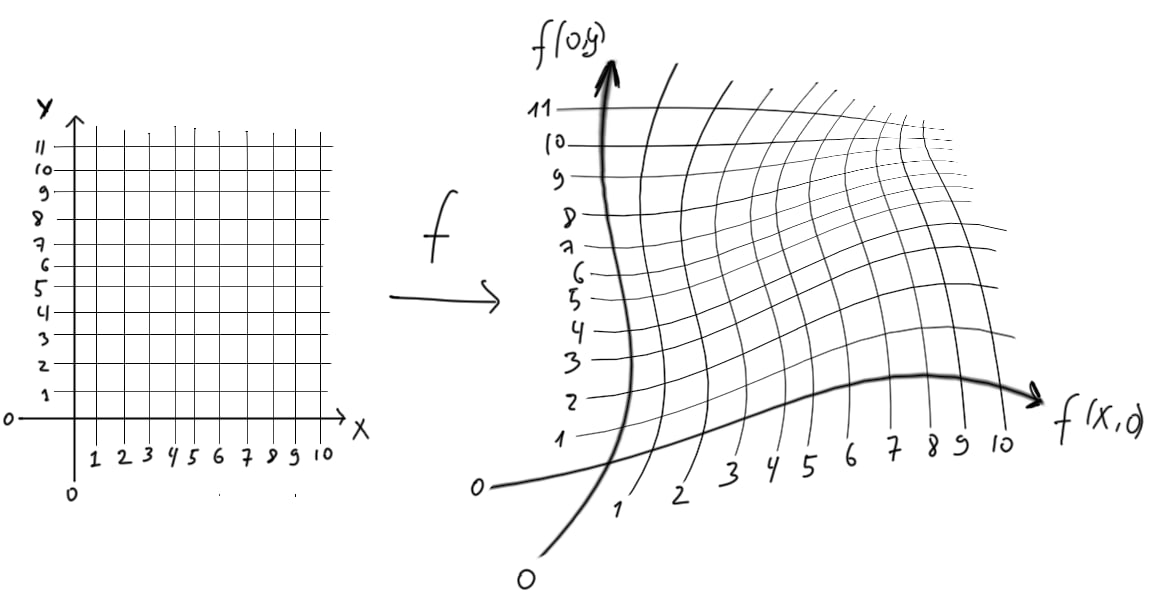
\includegraphics[scale =0.7]{deff2.jpg}
    \caption{Пример нелинейного отображения.}
    \label{deff2}
\end{figure}

Можно рассмотреть, например, и что-то более экзотическое, как показано на рисунке \ref{deff1}.

\begin{figure}
    \centering
    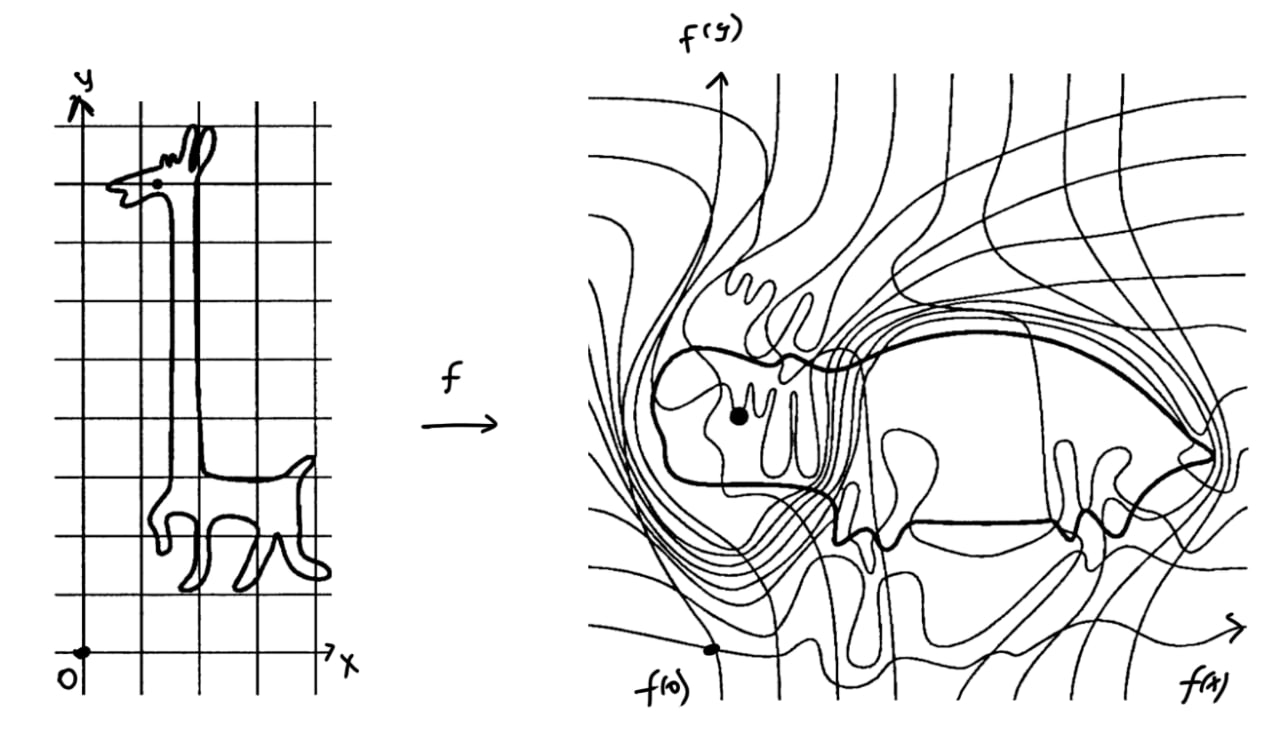
\includegraphics[scale = 0.5]{deff1.jpg}
    \caption{Пример нелинейного отображения: из жирафа получается бегемот.}
    \label{deff1}
\end{figure}

Однако же, это не означает, что линейную алгебру не надо изучать. Как раз наоборот, в сущности, анализ изучает любые подобное отображения с помощью линейной алгебры; локально они устроены как раз таки линейно (см. Рис.\ref{deff+linear}).

\begin{figure}
    \centering
    \includegraphics[scale = 0.7]{deff+linear.jpg}
    \caption{Вблизи это трудное отображение очень похоже на линейное.}
    \label{deff+linear}
\end{figure}




\section{Метрические пространства}

Определим \textit{метрическое пространство.} Пусть $E$ -- некоторое множество. \textit{Расстояние} в $E$ есть отображение $d:E\times E \to \mathbb{R}_{\ge 0}$, обладающее следующими свойствами:
\begin{enumerate}
    \item $d(x,y) = 0$, если и только если $x = y$.
    \item $d(x,y)=d(y,x)$, для любых $x,y \in E$.
    \item $d(x,z) \le d(x,y) + d(y,z)$, для любых трёх $x,y,z\in E$ (\textit{неравенство треугольника}).
\end{enumerate}

\subsection{Примеры расстояний}

 \begin{enumerate}
     \item Функция $d(x,y):=|x-y|$ есть расстояние в множестве $\mathbb{R}$ действительных чисел.
     \item В $\mathbb{R}^2$ обычное евклидово расстояние определяется формулой
     \[
       d(\m{x}, \m{y}):= \sqrt{(x_1 -y_1)^2 + (x_2 - y_2)^2},
     \]
     где $\m{x} = (x_1,x_2)$, $\m{y} = (y_1,y_2).$
     \item На плоскости $\mathbb{R}^2$ можно также ввести расстояние следующим образом:
     \[
      d(\m{x},\m{y}):= |x_1-y_1| + |x_2-y_2|.
     \]
     \item Ещё один пример расстояния на плоскости:
     \[
       d(\m{x},\m{y}):=\max\{|x_1 - y_1|, |x_2 - y_2|\}.
     \]
 \end{enumerate}

\subsection{Изометрия}~

Пусть $E,E'$ -- два метрических пространства, $d,d'$ -- расстояния в $E$ и $E'$. Биективное отображение $f:E \to E'$ называется \textit{изометрией}, если
\[
 d'(f(x), f(y)) = d(x,y)
\]
для любой пары элементов пространства $E$ обратное отображение $f^{-1}$ является изометрией пространства $E'$ на $E$. Два метрических пространства называются $E,E'$ \textit{изометричны}, если существует изометрия $E$ на $E'$.


Пусть $E$ -- метрическое пространство, $d$ -- расстояние в $E$ и $f$ -- биективное отображение $E$ на какое-то множество $E'$\footnote{в $E'$ до этого расстояние могло быть и не определено.} Мы можем тогда определить в $E'$ расстояние $d'$ как выше, \ie
\[
 d'(f(x), f(y)) = d(x,y),
\]
и в таком случае $f$ будет изометрией пространства $E$ в $E'$. Говорят, что расстояние $d'$ было \textit{перенесено} с $E$ на $E'$ отображением $f.$

\subsection{Расширенная действительная прямая $\overline{\mathbb{R}}$ и как измерять расстояние до бесконечности}~

Функция $f$, определённая на $\mathbb{R}$ условием 
\[
f(x) = \frac{x}{1+ |x|},
\]
является биективным отображением $f:\mathbb{R} \to (-1,1)$. Обратное отображение определяется формулой 
\[
 f^{-1}(x) = \frac{x}{1- |x|}
\]
при $|x|<1.$

Обозначим через $\overline{\mathbb{R}}$ множество, являющееся объединением $\mathbb{R}$ и двух новых элементов, обозначаемых символами $+\infty$ и $- \infty$ (=\textit{бесконечные точки}).

Тем самым, мы имеем вложение (инъекцию) $\mathbb{R} \hookrightarrow \overline{\mathbb{R}}$. Продолжим $f$ до биективного отображения $\overline{f}: \overline{\mathbb{R}} \to [0,1]$, полагая
\[
\overline{f}(x) = \begin{cases}
    f(x), & x \in \mathbb{R},\\
    1, & x = \infty,\\
    -1, & x = - \infty.
\end{cases}
\]

Тогда
\[
\overline{f^{-1}}(x) = \begin{cases}
    f^{-1}(x), & x \in (0,1),\\
    \infty, & x = 1,\\
    -\infty, & x = - 1.
\end{cases}
\]

Теперь мы можем ввести расстояние на $\overline{\mathbb{R}}$, $\overline{d}(x,y):=|\overline{f}(x) - \overline{f}(y)|$, $x,y \in \overline{\mathbb{R}}.$ Более подробно,
\begin{eqnarray*}
    \overline{d}(x,y) &=& \left| \frac{x}{1+|x|} - \frac{y}{1+|y|} \right|, \qquad x,y\in \mathbb{R}\\
    d(x, + \infty) &=& \frac{1}{1+|x|}, \qquad x \ge 0\\
    d(-\infty,x) &=& \frac{1}{1+|x|}, \qquad x \le 0.
\end{eqnarray*}

На $\overline{R}$ введём отношение порядка, по определению считая неравенство $x \le y$ эквивалентным неравенству $f(x) \le f(y)$. Легко проверить, что когда $x,y \in \mathbb{R}$, это отношение порядка есть обычное отношение порядка на $\mathbb{R}$ и что, кроме того, для любого $x\in \mathbb{R}$ мы имеем $- \infty < x < \infty.$

Действительные числа называются также \textit{конечными} элементами $\overline{\mathbb{R}}.$ 


\subsection{Шары и сферы}~

Элементы метрического пространства будем также называть \textit{точками}. 

\begin{definition}
    Пусть $E$ -- метрическое пространство с расстоянием $d$, а \textit{открытым шаром} (соотв. \textit{замкнутым шаром, сферой}) с центром в точке $a \in E$ и радиусом $r \in \mathbb{R}^+$ называется множество $B(a,r):=\{x\in E,\ |\, d(a,x)<r\}$ (соответственно, $\overline{B}(a,r):= \{x\in E\, |\, d(a,x) \le r\}$, $S(a,r):=\{x \in E\, |\, d(a,x) = r \}$).
\end{definition}

\begin{example}~
    \begin{enumerate}
        \item На действительной прямой $\mathbb{R}$ с расстоянием $d(x,y):=|x-y|$ имеем
        \[
         B(a,r) = (a-r, a+r), \qquad \overline{B}(a,r) = [a-r, a+r], \qquad S(a,r) = \{a-r, a+r\}.
        \]
        \item На расширенной прямой $\overline{\mathbb{R}}$ имеем
        \[
         B(+\infty, r) = \left(\frac{1-r}{r}, +\infty \left. \right. \right].
        \]
    \end{enumerate}
\end{example}


\subsection{Открытые множества и окрестности}~

\begin{definition}\label{def_of_open}
    \textit{Открытым множеством} в метрическом пространстве $E$ с расстоянием $d$ называется подмножество $A \subseteq E$, обладающее следующим свойством: для любой точки $x \in A$ существует такое $r >0$, что $B(x,r) \subseteq A$. Пустое множество открыто; всё пространство $E$ открыто. 
\end{definition}

\begin{lemma}\label{open_ball=open}
    Любой открытый шар в пространстве $E$ с расстоянием $d$ является открытым множеством.
\end{lemma}
\begin{proof}
    Пусть $B(a,r)$ -- открытый шар, по аксиоме выбора мы можем взять точку $x \in B(a,r)$, $x \ne a$. Тогда по определению $d(x,a) < r$. Рассмотрим теперь открытый шар $B(x,\delta)$, где $0 < \delta < r- d(a,x).$ Покажем, что $B(x,\delta ) \subseteq B(a, r)$, это и докажет лемму.

    По аксиоме выбора мы можем взять такое $y \in B(a,\delta)$, что $d(x,y)<\delta < r - d(a,x) $, тогда по неравенству треугольника
    \[
      d(a,y) \le d(a,x) + d(x,y) < d(a,x) + r - d(a,x) = r, 
    \]
    \ie $y\in B(a,r)$, что и доказывает $B(x,\delta) \subseteq B(a,r)$. Так как точка $x$ была выбрана произвольной в шаре $B(a,r)$, это показывает, что для любой точки в шаре мы нашли такой открытый шар, который целиком лежит в $B(a,r)$, \ie он открыт.
\end{proof}

\begin{lemma}\label{union_and_cap_of_open}
    Объединение любого семейства открытых множеств открыто и пересечение конечного числа открытых множеств открыто. 
\end{lemma}
\begin{proof}\
 
(1) Пусть $\mathscr{U} = \cup_{\alpha \in A}\mathscr{U}_\alpha$ и пусть $x \in \mathscr{U}$, тогда для какого-то $\alpha \in A$, $x \in \mathscr{U}_a$. Так как $\mathscr{U}_\alpha$ -- открыто, то найдётся такой $r >0$, что $B(x, r ) \subseteq \mathscr{U}_\alpha \subseteq \cup_{\alpha \in A}\mathscr{U}_\alpha$, что и доказывает открытость $\mathscr{U}.$

(2) Достаточно доказать, что множество двух открытых множеств $\mathscr{U}_1, \mathscr{U}_2$ открыто, а затем провести индукцию. Если $x \in \mathscr{U}_1 \cap \mathscr{U}_2$, то найдутся такие $r_1, r_2 >0$, что $B(x, r_1) \subseteq \mathscr{U}_1$, $B(x, r_2) \subseteq \mathscr{U}_2$. Очевидно, что $B(x, r) \subseteq \mathscr{U}_1 \cap \mathscr{U}_2$, где $r:= \min(r_1, r_2)$, что и доказывает открытость пересечения.
\end{proof}

\begin{definition}
    Пусть $A$ -- непустое множество в метрическом пространстве $E$ с расстоянием $d$. \textit{Открытой окрестностью} множества $A$ называется любое открытое множество $\mathscr{U}(A)$, содержащее $A$. В случае, когда $A = \{x\}$, мы говорим об окрестности $\mathscr{U}(x)$ точки $x$ (а не множества $\{x\}).$
\end{definition}

\begin{mydanger}{\bf{!}}
 Очевидно, что $\mathscr{U}(x)$ можно отождествить с подходящим открытым шаром $B(x,r)$, поэтому иногда мы не будем делать разницу между открытым шаром с центром в точке $x$ и открытым множеством, содержащим эту же точку $x.$    
\end{mydanger}

\subsection{Непрерывные отображения}

\begin{definition}
    Пусть $E$, $E'$ -- два метрических пространства, $d$ и $d'$ -- расстояния в них. Отображение $f:E \to E'$ называется \textit{непрерывным в точке $x_0 \in E$}, если для каждой окрестности $\mathscr{U}'$ точки $f(x_0) \in E'$ существует такая окрестность $\mathscr{U}(x_0)$ в $E$, что $f(\mathscr{U}(x_0)) \subseteq \mathscr{U}'(f(x_0))$. Отображение $f$ называется \textit{непрерывным в $E$} (или просто непрерывным), если оно непрерывно в каждой точке пространства $E.$
\end{definition}

Это же определение можно переформулировать и таким образом:

\begin{definition}
    Отображение $f:E \to E'$ непрерывно в точке $x_0$, если для любого шара $B(f(x_0), r) \subseteq E'$ всегда можно найти такой шар $B(x_0, \delta) \subseteq E$, что $f(B(x_0, \delta)) \subseteq B(f(x_0), r)$.
\end{definition}

Можно ещё вот так сказать:

\begin{definition}\label{reform_of_cont}
    Для того, чтобы отображение $f:E \to E'$ было непрерывно в точке $x_0 \in E$, необходимо и достаточно, чтобы для всякого $\varepsilon>0$ существовал такой $\delta >0$, что из $d(x_0,x)<\delta$ следует $d'(f(x),f(x_0))<\varepsilon$.
\end{definition}

\begin{figure}[h!]
    \centering
    \includegraphics[scale=0.5]{continous3.jpg}
    \caption{График отображения $f: \mathbb{R}^2 \to \mathbb{R}$ есть некоторая поверхность в $\mathbb{R}^3$. Нужно понимать, что мы горизонтальную плоскость отображаем в вертикальную прямую. Здесь показано, почему в точке $\m{a}\in \mathbb{R}^2$ это отображение непрерывно, $f(\m{a}) = A$. Какой бы оранжевый шар $\textcolor{orange}{B(A, \varepsilon)} \subseteq \mathbb{R}$ мы не взяли, можно найти синий шар $\textcolor{blue}{B(\m{a},r)} \in \mathbb{R}^2$ такой, что его образ $f( \textcolor{blue}{B(\m{a}, r)} )$ в вертикальной прямой (синяя полоска в оранжевом отрезке) будет целиком содержаться в этом оранжевом шаре.}
    \label{fig:enter-label}
\end{figure}


\begin{remark}\label{not_continous}
    Тогда если $f(x)$ не является непрерывным в точке $x_0$, то какой бы шар $B(x_0, \delta) \subseteq E$ мы не выбрали, всегда можно найти такой шар $B(f(x_0),r)$, что $f(x) \notin B(f(x_0),r)$ для каких-то $x \in B(x_0, \delta).$
\end{remark}


\begin{example}\label{x^2sin(1x)}
    Пусть $E = E' = \mathbb{R}$ с одинаковой метрикой $d(x,y) = |x-y|$, покажем, что отображение $\overline{f}:E \to E'$;
    \[
     \overline{f}(x) = \begin{cases}
         x^2 \sin \frac{1}{x}, & x \ne 0, \\
         0, & x =0
     \end{cases}
    \]
    непрерывно в точке $0$.

    Это значит, что для любого $\varepsilon >0$ мы должны найти такую $\delta >0$, что из неравенства $|x|<\delta$ будет следовать $|\overline{f}(x) - \overline{f}(0)| <\varepsilon.$ Чтобы найти такую $\delta$, мы заметим, что 
    \[
    \left|\overline{f}(x) -\overline{f}(0)\right| = \left|x^2 \sin \frac{1}{x} - 0 \right| = \left|x^2 \sin \frac{1}{x}\right| \le |x^2| = x^2,
    \]
поэтому если $x^2 <\varepsilon$, \ie $-\sqrt{ \varepsilon} <x < \sqrt{\varepsilon}$, то и $|\overline{f}(x) - \overline{f}(0)| <\varepsilon$. Значит, для любого $0 < \delta < \sqrt{\varepsilon}$ из неравенства $|x|<\delta$ вытекает неравенство $|\overline{f}(x) - \overline{f}(0)|$, что и доказывает непрерывность в точке $0.$
\end{example}

\begin{theorem}\label{preimage_of_open}
    Отображение $f:E \to E'$ между метрическими пространствами непрерывно тогда и только тогда, когда прообраз любого открытого в $E'$ открыт в $E.$
\end{theorem}
\begin{proof}~

(1) Пусть $f:E \to E'$ непрерывно. Возьмём открытое $\mathscr{U}' \subseteq E'$ и покажем, что $\mathscr{U}:=f^{-1}(\mathscr{U'})$ открыто в $E$. Пусть $x \in \mathscr{U}$, тогда $f(x) = x' \in \mathscr{U}'$, так как $\mathscr{U}'$ -- открыто в $E'$, то найдётся шар $B'(x',r') \subseteq \mathscr{U}'$. Так как шар $B'(x',r')$ есть открытая окрестность точки $x'$ и по предположению $f$ непрерывна и в точке $x \in E$, значит, найдётся такой шар $B(x,r) \subseteq E$ такой, что $f(B(x,r)) \subseteq B'(x',r')$. 

Таким образом, мы имеем $f(B(x,r)) \subseteq B'(x',r') \subseteq \mathscr{U}' .$ С другой стороны, если $A'\subseteq B' \subseteq E'$, то ясно, что $f^{-1}(A') \subseteq f^{-1}(B')$. Действительно, по определению прообраза
    \[
     f^{-1}(A'):= \{x \in X\, |\, f(x) \in A' \subseteq B'\} \Longrightarrow f^{-1}(A') \subseteq f^{-1}(B').
    \]

 Итак, мы получили, что $f(B(x,r)) \subseteq B'(x',r') \subseteq \mathscr{U}'$, тогда
 \[
  f(B(x,r)) \subseteq \mathscr{U}' \Longleftrightarrow f^{-1}(f(B(x,r))) \subseteq f^{-1}(\mathscr{U}')  \Longleftrightarrow B(x,r) \subseteq \mathscr{U},
 \]
 \ie для любого $x \in \mathscr{U}$ мы нашли шар $B(x,r)$, который целиком находится в $\mathscr{U}$, а это и означает, что $\mathscr{U}$ открыто.

(2) Пусть прообраз любого открытого есть открытое множество в $E.$ Пусть $\mathscr{U}'$ -- открытое в $E'$. Аксиома выбора позволяет нам выбрать точку $x' \in \mathscr{U}'$. Тогда для произвольно выбранной точки $x'$ существует такой открытый шар $B'(x',r')$, что $B'(x',r') \subseteq \mathscr{U}'.$

Пусть $f(x) = x'$, \ie $x \in f^{-1}(B'(x',r'))$. По предположению $f^{-1}(B'(x',r'))$ открыто в $E$. Это значит, что для любой выбранной точки $y \in f^{-1}(B'(x',r'))$ можно найти такой открытый шар $B(y,r)$, что $B(y,r) \subseteq f^{-1}(B'(x',r'))$. В частности, $B(x,r) \subseteq f^{-1}(B'(x',r'))$ 

Вспоминая, что если $A \subseteq B$, то и $f(A) \subseteq f(B)$. Тогда получаем 
\[
  B(x,r) \subseteq f^{-1}(B'(x',r')) \Longrightarrow f(B(x,r)) \subseteq f(f^{-1}(B'(x',r'))) \subseteq B'(x',r'),
\]
\ie для любого открытого шара $B'(x',r')$, где $x' = f(x)$, мы нашли такой открытый шар $B(x,r)$, что $f(B(x,r)) \subseteq B'(x',r')$, но это и означает непрерывность.
\end{proof}

\begin{corollary}
    Отображение $f:E \to E'$ -- непрерывно в точке $x$, тогда и только тогда, когда прообраз любого открытого шара $B(f(x),r) \subseteq E'$ -- открытое множество в $E$
\end{corollary}
\begin{proof}
    Это сразу следует из предыдущей теоремы и леммы \ref{union_and_cap_of_open}.
\end{proof}

\begin{theorem}\label{comp_of_continous}
    Пусть $E,E,E''$ -- метрические пространства и пусть $f:E \to E'$, $g:E' \to E''$ -- отображения. Если $f$ непрерывно в точке $x_0$ и $g$ непрерывно в $f(x_0)$, то $h = g \circ f$ непрерывно в точке $x_0.$ Если $f$ непрерывно в $E$ и $g$ непрерывно в $E'$, то $h$ непрерывно в $E.$
\end{theorem}
 \begin{proof}
     Второе утверждение, очевидно, следует из первого. Пусть $\mathscr{U}''$ -- окрестность точки $h(x_0) =  g(f(x_0))$. Тогда из предположения о непрерывности и Теоремы \ref{preimage_of_open} следует, что $\mathscr{U}':=g^{-1}(\mathscr{U}'')$ -- открытое множество в $E'$, содержащее точку $f(x_0)$. Далее, так как $f$ непрерывно, то по теореме \ref{cap_of_intervals}, прообраз $\mathscr{U}:=f^{-1}(\mathscr{U}')$ -- открытое множество, содержащее точку $x_0$. Таким образом, $h^{-1}(\mathscr{U}'') = \mathscr{U}$ открытое, тогда по теореме \ref{preimage_of_open}, $h$ непрерывно в точке $x_0$, что и завершает доказательство. 
 \end{proof}


\begin{corollary}\label{restriction}
    Если $f$ -- отображение метрического пространства $E$ в метрическое пространство $E'$, непрерывное в точке $x_0$, и $A \subseteq E$, $A \ni x_0$, то сужение $f|_A:=f \circ \mathrm{in}_A$ также непрерывно в $x_0,$ где $\mathrm{in}_A:A \hookrightarrow E$ -- вложение.
\end{corollary}
\begin{proof}
    На самом деле, $f$ непрерывно в $x_0$ по условию, а $\mathrm{in}_A$ непрерывно в любой точке $a \in A$, тогда из предыдущей теоремы и следует утверждение.
\end{proof}

 \begin{remark}\label{+infty}
    Пусть $E = \overline{\mathbb{R}}$ -- расширенная прямая, рассмотрим выражение $\lim_{x \to +\infty, x \in \mathbb{{R}}}f(x) = a'$, где $f:\mathbb{R} \to E' $ -- некоторое отображение. Мы знаем, что $B(+\infty, \delta) = (\frac{1-\delta}{\delta}, \infty]$. Тогда непрерывность в точке $+\infty$ означает, что для любого $r >0$ найдётся такая $\delta>0$, что $f((\frac{1-\delta}{\delta}, \infty]) \subseteq B(a',r)$. Другими словами, для любого шара $B(a',r)$ найдётся такое число $\alpha \in \mathbb{R}$, что $f(\beta) \in B(a',r)$ для всех $\beta > \alpha.$
\end{remark}

\section{Замкнутые множества, точки замыкания (=точки прикосновения), замыкание множества.}

\begin{definition}
    \textit{Замкнутое множество} в метрическом пространстве $E$ есть дополнение открытого множества. 
\end{definition}

Пустое множество замкнуто, замкнуто и всё пространство $E$.

\begin{example}
    Пусть $E = \mathbb{R}$, $d(x,y):= |x-y|$. Тогда промежутки $[a, + \infty)$, $(- \infty,a]$ замкнуты, потому что 
    \[
     [a, + \infty) = \mathbb{R} \setminus \cup_{n \ge 1} (a-n, a)
    \]
\end{example}





\begin{definition}\label{limit_point_in_metric}
  Пусть $E$ -- метрическое пространство, $d$ -- расстояние в нём, и пусть $A \subseteq E$. \textit{Точка замыкания} (=\textit{точка прикосновения}) множества $A$ -- такая точка $x \in E$, каждая окрестность которой имеет с $A$ непустое пересечение. Множество всех точек замыкания называется \textit{замыканием} множества $A$ и обозначается символом $\overline{A}.$
\end{definition}

\begin{example}~
    \begin{enumerate}
        \item $E= \mathbb{R}$ с обычной метрикой $d(x,y) = |x-y|$, $A = (0,1]$, тогда $0$ -- точка замыкания, потому что любой шар $B(0,r) = (-r,r) \cap A \ne \varnothing$.
        \item На расширенной прямой $\overline{\mathbb{R}}$ шары $B(+\infty, r) = (\frac{1-r}{r}, +\infty)$ есть просто луч. Ясно, что $B(+\infty, r)\cap \mathbb{R} \ne \varnothing$, \ie это и означает, что замыкание множества $\mathbb{R}$ и даст расширенную прямую $\overline{\mathbb{R}}.$
    \end{enumerate}
\end{example}

\begin{lemma}\label{closure_in_metric}
    Множество $F$ в метрическом пространстве замкнуто, если и только если все его точки это предельные точки, \textit{т.е.,} $F = \overline{F}.$ 
\end{lemma}
(1) Пусть $F$ -- замкнуто, тогда найдётся какое-то открытое $\mathscr{U} \subseteq E$, такое, что $F  = E \setminus \mathscr{U}$. Пусть $x \notin F$, тогда $x \in \mathscr{U}$, и тогда найдётся окрестность $\mathscr{W}(x)$ такая, что $\mathscr{W}(x) \subseteq \mathscr{U}$, потому что $\mathscr{U}$ -- открыто, \textit{т.е.,} $\mathscr{W}(x) \cap F = \varnothing.$ Таким образом, получили, что если $F$ -- замкнуто, то никакая точка $x \notin F$ не может быть предельной для $F$, \textit{т.е.,} $F = \overline{F}.$ 

(2) Пусть $F = \overline{F}$, тогда для любой точки $x \notin F$, можно всегда найти окрестность $\mathscr{W}(x)$ такую, что $\mathscr{W}(x) \cap F = \varnothing$. Пусть $\mathscr{U}:= \cup_{x E\setminus F} \mathscr{W}(x)$, тогда, $\mathscr{U}$ -- открыто в $E$ и $F = E \setminus \mathscr{U}.$


\begin{lemma}\label{preimage_of_closed}
    Отображение $f:E \to E'$ между метрическими пространствами непрерывно тогда и только тогда, когда прообраз любого замкнутого множества в $E'$ есть замкнутое множество в $E.$
\end{lemma}

\begin{proof}
    Пусть $F'$ -- замкнутое подмножество в $E'$, тогда $\mathscr{U}': = E'\setminus F'$ -- открыто в $E'$ и $E' = F' \cup \mathscr{U}'$, $F' \cap \mathscr{U}' = \varnothing$. Далее, ясно что $f^{-1}(F') \cap f^{-1}(\mathscr{U}') = \varnothing$ и $E = f^{-1}(F') \cap f^{-1}(\mathscr{U}')$. Тогда согласно Теореме \ref{preimage_of_open}, $f$ -- непрерывно если и только если $f^{-1}(\mathscr{U}')$ -- открыто в $E$, но тогда $f^{-1}(F') = E \setminus \mathscr{U}'$ замкнуто тогда и только тогда, когда $f^{-1}(\mathscr{U}')$ -- открыто. Это завершает доказательство.
\end{proof}

\begin{lemma}\label{closed_ball=closed}
    Замкнутый шар -- замкнут.
\end{lemma}
\begin{proof}
Пусть $(E,d)$ -- метрическое пространство, $\bar B(a,r)$ -- замкнутый шар. Покажем, что $E\setminus B(a,r)$ -- открыто. Пусть $x\notin \bar B(a,r)$, тогда $d(a,x) > r$, и положим $\varepsilon: = d(a,x) - r$, очевидно, что $\varepsilon >0$. Имеем $d(x,a) \le d(y,a) + d(y,x)$, тогда $d(y,a) \ge d(x,a) - d(y,x)$.

Пусть теперь $y\in B(x, \frac{\varepsilon}{2})$, тогда получаем
\begin{eqnarray*}
    d(y,a) &\ge & d(x,a) - d(y,x) \\
    &\ge & r + \varepsilon- \frac{\varepsilon}{2}\\
    &=& r + \frac{\varepsilon}{2}\\
    &>& r
\end{eqnarray*}
\textit{т.е.,} $y\notin \bar B(a,r)$. А это означает, что весь открытый шар $B(x, \frac{\varepsilon}{2})$ не лежит в $\bar B(a,r)$, что и требовалось доказать.
\end{proof}



\section{Подпространства метрического пространства}

Пусть $F \subseteq E$ -- непустое подмножество метрического пространства $E$ с расстоянием $d$, тогда $F \times F \subseteq E \times E$ -- непустое подмножество, тогда мы имеем следующую коммутативную диаграмму

\[
  \begin{tikzcd}
    F \times F \arrow[hook]{d}[left]{\mathrm{in}} \arrow{dr}{d|_{F \times F}} &  \\
    E \times E \arrow{r}[below]{d} & \mathbb{R}
  \end{tikzcd}
\]
\ie, \textit{сужая} метрику $d$ на $F$, мы получаем метрическое пространство $(F,d|_{F \times F})$, которое мы будем для простоты обозначать $(F, d_F)$.

\begin{definition}
    Метрическое пространство, определённое таким образом, называется \textit{подпространством} $F$ метрического пространства $E$.
\end{definition}

\begin{figure}[h!]
    \centering
    \includegraphics[scale = 0.4]{open_in_F.jpg}
    \caption{Пусть $E = \mathbb{R} \times \mathbb{R}$ -- обыкновенная плоскость с обыкновенной евклидовой метрикой $d(\m{x},\m{y}) = \sqrt{(x_1 - y_1)^2+ (x_2 - y_2)^2}$, и пусть $F = \mathbb{R}$, которую мы можем понимать как множество вида $\{(x,0), x\in \mathbb{R}\}$. На рисунке $F$ отождествлена с осью $Ox$. Тогда, сужая метрику $d$ на $F$, мы получаем, что $d(x,y) = \sqrt{(x-y)^2} = |x-y|$. Более того, ясно, что любой интервал $(a,b)$ можно получить, пересекая открытый круг с $F.$}
    \label{fig:enter-label}
\end{figure}


\begin{proposition}\label{open_in_subset}
    Для того чтобы множество $S \subseteq F$ было открыто в подпространстве $F$, необходимо и достаточно, чтобы существовало такое множество $\mathscr{U}$, открытое в $E$, что $S = \mathscr{U} \cap F.$
\end{proposition}

\begin{proof}
    Прежде всего, поймём, что есть открытый шар в $F$. Пусть $a \in F$, и рассмотрим открытый шар $B(a,r) \subseteq E$, тогда получаем
    \begin{eqnarray*}
        F \cap B(a,r) &:=& \{x \in E \cap F\, :\, d(x,a)<r\} \\
        &=&\{x\in F\, :\, d(x,a)<r\} \\
        &=& \{x \in F\, :\, d_F(x,a)<r\},
    \end{eqnarray*}
    \ie $F \cap B(a,r)$ -- это \textbf{открытый шар в $F$ с центром в точке $a$ радиуса $r.$}

\begin{mydanger}{\bf{!}}
    Обратим внимание, что если $F = \mathbb{R}_{\ge 0} \subseteq \mathbb{R} = E$, $d(x,y) = |x-y|$, то, например, $[0,1)$ -- открытый шар в $F = \mathbb{R}_{\ge 0}$, так как $[0,1) = (-1,1) \cap \mathbb{R}_{\ge 0}$. Hо! В $\mathbb{R}$, $[0,1)$ и не открыт и не замкнут!
\end{mydanger}

(1) Пусть $\mathscr{U}$ -- открытое множество в $E$, и пусть $x \in \mathscr{U} \cap F$. Так как $\mathscr{U}$ -- открытое в $E$, то найдётся шар $B(x,r) \subseteq E$ такой, что $B(x,r) \subseteq \mathscr{U}$. Тогда $F \cap B(x,r) \subseteq F \cup \mathscr{U}$. Но мы уже поняли, что $B(x,r) \cap F$ -- открытый шар в $F$, но тогда включение $F \cap B(x,r) \subseteq F \cup \mathscr{U}$ и означает, что $\mathscr{U} \cap F$ открыто в $F$, ибо $x$ -- произвольная точка в $\mathscr{U} \cap F.$

(2) Пусть $S$ открыто в $F$, это значит, что для любой точки $x \in S$ можно найти открытый шар $B(x, r(x)) \subseteq E$ такой, что $F \cap B(x,r(x)) \subseteq S$ (т.к., $F \cap B(x,r(x))$ -- это открытый шар в $F$).

Тогда 
\[
 S = \bigcup_{x \in S} F \cap B(x, r(x)) = F \cap \mathscr{U},
\]
где $\mathscr{U} = \cup_{x\in S} B(x, r(x)) \subseteq E$, тогда по Леммам \ref{open_ball=open}, \ref{union_and_cap_of_open} $\mathscr{U}$ открыто в $E$.
\end{proof}

\section{Пределы}

Пусть $E$ -- метрическое пространство, $d$ -- расстояние в нём, пусть $A \subseteq E$ -- некоторое его подмножество, пусть $a$ -- точка замыкания для $A$, \ie $a \in \overline{A}$, и пусть $f:A \to E'$ некоторое отображение в метрическое пространство $E'.$

\begin{definition}\label{the_main_def_of_limit}
    Пусть $a \notin A$. Мы будем говорить, что $f(x)$ \textit{имеет предел $a' \in E'$ при $x \in A$, стремящемся к $a$ (или $a'$ есть предел отображения $f$ в точке $a\in \overline{A}$ по множеству $A$}), если отображение $\overline{f}:A \cup \{a\} \to E$, определённое условиями
    \[
     \overline{f}(x) = \begin{cases}
         f(x), & x \in A, \\
         a', & x = a,
     \end{cases}
    \]
    непрерывно в точке $a$.
\end{definition}

В этом случае, мы пишем
\[
 a' := \lim_{x\to a, x \in A} f(x).
\]

\begin{mydanger}{\bf{!}}
    Если $a \in A$, то мы пользуемся той же терминологией и теми же обозначениями как и в случае, когда отображение $f$ непрерывно в точке $a$, причём $a':=f(a).$
\end{mydanger}

\begin{example}~

 \begin{enumerate}
  \item Пусть $E = E'=\mathbb{R}$, $d(x,y) = d'(x,y): |x-y|$, $A = \mathbb{R}\setminus \{0\}$, и отображение $f: A \to \mathbb{R}$ задаётся с помощью $f(x) = x$. 

  Ясно, что $0$ есть точка замыкания для $A$, так как шар $B(0,r)$ с такой метрикой $d$ -- это просто интервал $(-r,r)$, тогда очевидно, что $(-r, r) \cap A = (-r, r)\setminus \{0\} \ne \varnothing$, что и доказывает, что точка $0$ -- точка замыкания для множества $A$.

  Пусть
  \[
   \overline{f}(x): = \begin{cases}
       x, & x \in A \\
       \alpha, & x =0.
   \end{cases}
  \]

Если мы поймём, при каком $\alpha$ это отображение $\overline{f}$ непрерывно в точке $0$, то мы и найдём предел, который и будет равен этому $\alpha.$

Итак, пусть $\overline{f}$ непрерывна в точке $0$, тогда для любого шара $B(\alpha, r) \subseteq E' = \mathbb{R}$ должен найтись шар $B(0,\delta) \subseteq E = \mathbb{R}$ такой, что $f(B(0,\delta)) \subseteq B(\alpha, r)$.

Ясно, что $B(0,\delta) = (-\delta, \delta)$, $B(\alpha, r) = (\alpha - r,\alpha + r)$, и 
\[
 \overline{f}(B(0,\delta)) = \overline{f}((-\delta, \delta)) = (-\delta, \delta) \setminus \{0\} \cup \{\alpha\},
\]
следовательно, если $\overline{f}$ будет непрерывной в точке $0$, то для любого $r >0$ можно найти $\delta >0$ такое, что
\[
 \overline{f}(B(0,\delta)) = (-\delta, \delta) \setminus \{0\} \cup \{\alpha\} \subseteq (\alpha - r, \alpha + r),
\]
тогда $-\delta, \delta \in (\alpha - r, \alpha + r)$. Это значит, что $\alpha -r < 0$, $\alpha + r >0$. Таким образом, если $\alpha \ne 0$, \textbf{то только для шаров вида (\ie не для всех!) $B(\alpha, r)$, где $\alpha -r < 0$, $\alpha + r >0$,} всегда найдётся шар $B(0,\delta)$ такой, что $f(B(0,\delta)) \subseteq B(\alpha, r)$, \ie при $\alpha \ne 0$ отображение $\overline{f}$ не будет непрерывным в $0$. С другой стороны, если же $\alpha =0$, то мы получаем неравенства $-r <0$, $r>0$, которые выполняются всегда, так как мы требуем чтобы $r>0$.

Таким образом, $\lim_{x\in 0, x \in A}f(x) = 0.$

 \item Пусть $E = E' = \mathbb{R}$ с расстоянием $d(x,y) = |x-y|$, $A = \mathbb{R}\setminus \{0\}$, $f(x): = x^2 \sin \frac{1}{x}.$ Тогда, как мы уже видели в примере \ref{x^2sin(1x)}, отображение  
     \[
     \overline{f}(x) = \begin{cases}
         x^2 \sin \frac{1}{x}, & x \ne 0, \\
         0, & x =0
     \end{cases}
    \]
    непрерывно в точке $x = 0$, тогда $\lim_{x \to 0, x \in A}f(x) = 0.$
 \end{enumerate}
    
\end{example}

Вспомнив определение непрерывности и точки замыкания, определение предела можно переформулировать следующими двумя эквивалентными способами:

\begin{definition}
    $\lim_{x \to a, x \in A}f(x) = a'$ эквивалентно тому, что для любого шара $B(a',r) \subseteq E'$ найдётся такой шар $B(a,\delta) \subseteq A$, что $f(B(a,\delta)\cap A) \subseteq B(a',r)$.
\end{definition}
\begin{mydanger}{\bf{!}}
    Так как $a$ -- точка замыкания, то множество $A \cap B(a,\delta)$ никогда не пусто для любого $\delta >0$.
\end{mydanger}




































\begin{definition}\label{def_for_cont_via_d-e}
    $\lim_{x \to a, x \in A}f(x) = a'$ эквивалентно тому, что для каждого $\varepsilon>0$ можно найти такое $\delta >0$, что из $x \in A$ и $d(x,a)<\delta$ следует $d'(a',f(x))<\varepsilon.$
\end{definition}

\begin{proposition}
    Отображение может иметь лишь один предел по множеству $A$ в данной точке $a \in \overline{A}.$
\end{proposition}
\begin{proof}
    Пусть  $\lim_{x \to a, x \in A}f(x) = a'$ и  $\lim_{x \to a, x \in A}f(x) = b'$, при этом $a' \ne b'$. Тогда, согласно Определению \ref{def_for_cont_via_d-e}, 
 \begin{enumerate}
     \item  $\lim_{x \to a, x \in A}f(x) = a'$ означает, что для любого $\varepsilon >0$ можно найти такое $\delta_1 >0$, что из $x \in A$ и $d(x,a)<\delta_1$ следует $d'(a',f(x))<\varepsilon$
     \item $\lim_{x \to a, x \in A}f(x) = b'$ означает, что для того же $\varepsilon >0$ можно найти такое $\delta_2 >0$, что из $x \in A$ и $d(x,a)<\delta_2$ следует $d'(b',f(x))<\varepsilon$.
 \end{enumerate}
Тогда по неравенству треугольника
\[
 d'(a',b') \le d'(a', f(x)) + d'(f(x), b') < 2\varepsilon,
\]
\ie расстояние между фиксированными точками $a',b' \in E'$ может быть любым, что невозможно если $a' \ne b'.$
\end{proof}

Из определения предела вытекает:
\begin{theorem}[{Критерий непрерывности}]\label{criteria_of_continous}
    Пусть $f$  -- отображение метрических пространств $f:E \to E'$. Для того чтобы $f$ было непрерывно в точке $x_0 \in E$, являющейся точкой замыкания множества $E\setminus\{x_0\}$, необходимо и достаточно, чтобы $f(x_0) = \lim_{x \to x_0, x\in E \setminus \{x_0\}}f(x).$
\end{theorem}
\begin{proof}
    Это лишь пересказ определения.
\end{proof}

\begin{theorem}\label{limit_for_any_subset}
    Пусть $a' = \lim_{x \to a, x \in A} f(x)$. Тогда для каждого подмножества $B \subseteq A$, для которого $a \in \overline{B}$, $a' = \lim_{x \to a, x \in B}f(x)$.
\end{theorem}

\begin{proof}
    Это сразу следует из определения предела и следствия \ref{restriction}.
\end{proof}

\begin{theorem}\label{lim_of_composition}
    Пусть $E,E',E''$ -- метрические пространства, $A \subseteq E$, и $f:A \to E'$, $g:E' \to E''$ -- отображения. Если $\lim_{x \to a, x \in A}f(x) = a'$ и $g$ непрерывно в точке $a'$, то $g(a') = \lim_{x \to a, x \in A}g(f(x))$. 
\end{theorem}
\begin{proof}
    Это сразу следует из определения предела и теоремы \ref{comp_of_continous}.
\end{proof}

\begin{mydanger}{\bf{!}}
    В случае, когда $A = E$, мы будем вместо $\lim_{x \to a, x \in A}f(x)$  писать $\lim_{x \to a}f(x).$
\end{mydanger}

\begin{remark}
 Пусть $E = \overline{\mathbb{R}}$ -- расширенная прямая, рассмотрим выражение $\lim_{x \to +\infty, x \in \mathbb{{R}}}f(x) = a'$, где $f:\mathbb{R} \to E' $ - некоторое отображение. Мы знаем, что $B(+\infty, \delta) = (\frac{1-\delta}{\delta}, \infty]$. Тогда непрерывность в точке $+\infty$ означает, что для любого $r >0$ найдётся такой $\delta>0$, что $f((\frac{1-\delta}{\delta}, \infty]) \subseteq B(a',r)$. Другими словами, если $\lim_{x \to + \infty} f(x) = a'$, то для любого шара $B(a',r)$ найдётся такое число $\alpha \in \mathbb{R}$ что $f(\beta) \in B(a',r)$ для всех $\beta > \alpha.$ \textbf{Именно так мы и будем понимать запись $\lim_{x \to +\infty}f(x) = a'$};
 \[
  \boxed{ 
    \boxed{
    \lim_{x \to +\infty}f(x) = a' \Longleftrightarrow \forall r > 0\, \exists \alpha \in \mathbb{R}:\, f(\beta) \in B(a',r) \,\forall \beta >\alpha.
    }
}
 \]
\end{remark}

\begin{mydanger}{\bf{!}}
    В частности, если $E' = \mathbb{R}$ с обычной метрикой и $\mathbb{N} \subseteq \overline{\mathbb{R}}$, то $\lim_{x \to +\infty, x \in \mathbb{{N}}}f(x) =a'$ есть знакомое нам определение предела последовательности.
\end{mydanger}

\begin{lemma}\label{choice_of_seqeunce}
    Для любой точки $a \in \overline{A}$ существует такая последовательность $\{x_n\}$ точек из $A$, что $a = \lim_{n \to \infty} x_n$
\end{lemma}

\begin{proof}
    Так как $a$ -- точка замыкания, то любой шар $B(a, r)$ содержит хотя бы одну точку из $A$, \ie $B(a, r) \cap A \ne \varnothing$. В частности, для любого $n\ge 1$, $B(a, \frac{1}{n}) \cap A \ne \varnothing$. Тогда по Аксиоме Выбора, для каждого $n\ge 1$ мы можем выбрать $x_n \in B(a, \frac{1}{n})$. Покажем, что $\lim_{n \to \infty} x_n = a$. Действительно, пусть $n<m$, и мы имеем тогда $x_n \in B(a, \frac{1}{n})$, $x_m \in B(a, \frac{1}{m})$. 

    Тогда имеем
    \[
     d(x_n, x_m) \le d(a,x_n) + d(a,x_m) <\frac{1}{n} + \frac{1}{m} < \frac{2}{n}.
    \]

Это означает, что все $x_n, x_{n+1}, \ldots \in B(a, \frac{2}{n})$, что и доказывает требуемое.
\end{proof}

\begin{corollary}\label{Weirstrass_mega}
    Подмножество $F$ в метрическом пространстве $E$ замкнуто, тогда и только тогда, когда из любой последовательности $(x_n)$ в $F$, можно выбрать сходящуюся подпоследовательность $(x_{n_k})$, такую, что $\lim_{n\to \infty} x_{n_k} \in F$. 
\end{corollary}

\begin{proof}
    По Предложению \ref{closure}, $F$ замкнуто, если и только если $F = \overline{F}$. Тогда используя лемму \ref{choice_of_seqeunce}, мы завершаем доказательство. 
\end{proof}



\begin{theorem}\label{lim=>for_any_sequence}
    Пусть $f: A \to E'$ -- отображение множества $A \subseteq E$ в метрическое пространство $E'$ и $a \in \overline{A}.$ Для того, чтобы $f$ имело предел $a' \in E'$ в точке $a$ по $A$, необходимо и достаточно, чтобы для каждой последовательности $\{s_n\}$ точек из $A$, сходящейся к $a$, последовательность $f(s  _n)$ сходилась к $a'.$
\end{theorem}

\begin{proof}~

(1) Необходимость. 

Пусть $\lim_{x \to a, x \in A}f(x) = a'$, и пусть $s:\mathbb{N} \to {A}\cup \{a\}$ -- последовательность $\{s_n\}$. По условию, $\lim_{n \to \infty }s_n = a$ и так как $\lim_{x \to a, x \in A}f(x) = a'$, то по определению предела \ref{the_main_def_of_limit}, $\overline{f}$ непрерывна в точке $a$. Тогда по Теореме \ref{lim_of_composition}, последовательность $s':=\overline{f} \circ s: \mathbb{N} \to E'$, в которой $s'_n = f(s_n)$, имеет предел $\overline{f}(a) = a'$, что и доказывает необходимость.

(2) Достаточность.

Будем доказывать от противного. Пусть для любой последовательности $\{s_n\}$ точек из $A$, $\lim_{n \to \infty} s_n = a$ имеем $\lim_{n \to \infty}f(s_n) = a'$, но $a' \ne \lim_{x \to a, x\in A}f(x).$ Тогда  $\lim_{n \to \infty} s_n = a$ влечёт, что, начиная с какого-то номера $N$, $d(a,s_n) < \varepsilon$ для всех $n > N$.

С другой стороны, $a' \ne \lim_{x \to a, x\in A}f(x)$ означает, что $f(x)$ не является непрерывным в точке $a$. Тогда, существует такое $\varepsilon >0$, что для любого номера $n$ найдётся такая точка $x_n \in A$, удовлетворяющая двум условиям: $d(a,x_n) < \frac{1}{n}$ и $d'(a',f(x_n))\ge \varepsilon$. Но тогда последовательность $\{f(s_n)\}$ не сходится к $f(s)$, что противоречит условию.
\end{proof}


\begin{theorem}\label{f<g=>lim}
  Пусть $E$ -- метрическое пространство с метрикой $d$, и $\mathbb{R}$ -- рассматривается с обычной метрикой $d'(x,y): = |x-y|$.  Пусть $f,g:A \to \mathbb{R}$ -- функции такие что $f(x) \le g(x)$ для всех $x \in A$, тогда $\lim_{x\in A, x \to a}f(x) \le \lim_{x \in A, x \to a}g(x)$.
\end{theorem}

\begin{proof}
Пусть $\lim_{x\in A, x \to a}f(x) = \alpha$, $\lim_{x\in A, x \to a}g(x) = \beta$.

Тогда, по арифметике предела $\lim_{x\in A, x \to a}(g(x) - f(x)) = \beta - \alpha.$

Пусть $\alpha > \beta$. Пусть $\varepsilon : = \alpha - \beta$, тогда $\varepsilon >0$.

Из определения предела следует, что для выбранного $\varepsilon$, можно найти такое $\delta>0$, что из $d(x,a)<\delta$ будет следовать $|g(x) - f(x) - (\beta - \alpha)| < \varepsilon$, но тогда получаем, что
\[
 g(x) - f(x) < \varepsilon + (\beta - \alpha) = 0,
\]
что даёт противоречие. Это и доказывает утверждение.
\end{proof}

%\input{old/Rn}

\part{Семинарские занятия}
\chapter{Принцип полноты и последовательности}
%\section{Занятие \#1}

\subsection{Рациональные числа}

\begin{problem}
 Докажите, что число \(\sqrt{2} + \sqrt{3}\) иррационально.
\end{problem}

\begin{proof}[Решение]~

(1) Первый способ (от противного). 
Предположим, что \(\sqrt{2} + \sqrt{3}\) рационально. Тогда:
\[
\sqrt{2} + \sqrt{3} = r, \quad r \in \mathbb{Q}
\]
Возведем в квадрат:
\[
(\sqrt{2} + \sqrt{3})^2 = r^2 \implies 2 + 2\sqrt{6} + 3 = r^2 \implies 5 + 2\sqrt{6} = r^2
\]
Выразим \(\sqrt{6}\):
\[
\sqrt{6} = \frac{r^2 - 5}{2}
\]
Так как \(r\) рационально, то правая часть рациональна, но \(\sqrt{6}\) иррационально. Противоречие.

(2) Второй способ (через обратную величину).

Заметим:
\[
(\sqrt{2} + \sqrt{3})(\sqrt{3} - \sqrt{2}) = 3 - 2 = 1
\]
Предположим \(\sqrt{2} + \sqrt{3} = r \in \mathbb{Q}\). Тогда:
\[
\sqrt{3} - \sqrt{2} = \frac{1}{r} \in \mathbb{Q}
\]
Сложим два равенства:
\[
(\sqrt{2} + \sqrt{3}) + (\sqrt{3} - \sqrt{2}) = r + \frac{1}{r} \implies 2\sqrt{3} = r + \frac{1}{r}
\]
Отсюда \(\sqrt{3} = \frac{r^2 + 1}{2r} \in \mathbb{Q}\), но \(\sqrt{3}\) иррационально. Противоречие.

\end{proof}

\subsection{Бином Ньютона}


Напомним формулы бинома Ньютона.
\[
(a + b)^n = \sum_{k=0}^{n} C_n^k a^{n-k} b^k = \sum_{k=0}^{n} \binom{n}{k} a^{n-k} b^k
\]
где \(\binom{n}{k} = \frac{n!}{k!(n-k)!}\) -- биномиальный коэффициент.


\begin{figure}[h!]
    \centering
     \begin{tikzpicture}[scale=0.7]
\foreach \n in {0,...,5} {
  \foreach \k in {0,...,\n} {
    \node at (2*\k - \n, -\n) {\(\binom{\n}{\k}\)};
  }
}
\end{tikzpicture}
    \caption{Биномиальные коэффициенты удобно располагать в треугольнике Паскаля}
\end{figure}

\begin{mydanger}{\bf !}
При закрашивании нечётных чисел в треугольнике Паскаля возникает фрактальная структура, аналогичная треугольнику Серпинского.    
\end{mydanger}

\begin{problem}
    Раскройте скобки в выражении \((a + b)^7\).
\end{problem}

\begin{proof}[Решение]
\[
(a + b)^7 = \sum_{k=0}^{7} \binom{7}{k} a^{7-k} b^k
\]
Вычислим коэффициенты:
\begin{align*}
\binom{7}{0} &= 1, &\binom{7}{1} &= 7, &\binom{7}{2} &= 21, \\
\binom{7}{3} &= 35, &\binom{7}{4} &= 35, &\binom{7}{5} &= 21, \\
\binom{7}{6} &= 7, &\binom{7}{7} &= 1.
\end{align*}
Результат:
\[
(a + b)^7 = a^7 + 7a^6b + 21a^5b^2 + 35a^4b^3 + 35a^3b^4 + 21a^2b^5 + 7ab^6 + b^7
\]    
\end{proof}


\begin{problem}
    Найдите коэффициент при \(x^3\) в выражении \(\left( \sqrt{x} + \frac{1}{\sqrt[3]{x}} \right)^{16}\). 
\end{problem}
\begin{proof}[Решение]
Преобразуем:
\[
\sqrt{x} = x^{1/2}, \quad \frac{1}{\sqrt[3]{x}} = x^{-1/3}
\]
Общий элемент разложения:
\[
T_k = \binom{16}{k} (x^{1/2})^{16-k} (x^{-1/3})^k = \binom{16}{k} x^{\frac{16-k}{2} - \frac{k}{3}}
\]
Упростим показатель:
\[
\frac{16-k}{2} - \frac{k}{3} = \frac{3(16-k) - 2k}{6} = \frac{48 - 5k}{6}
\]
Решим уравнение:
\[
\frac{48 - 5k}{6} = 3 \implies 48 - 5k = 18 \implies 5k = 30 \implies k = 6
\]
Тогда, искомый коэффициент:
\[
\binom{16}{6} = \frac{16!}{6!10!} = \frac{16×15×14×13×12×11}{6×5×4×3×2×1} = \frac{5765760}{720} = 8008
\]    
\end{proof}


\subsection{Вычисление некоторых сумм}

\begin{problem}
    Вычислить сумму \(1 + 2 + \cdots + 100\).
\end{problem}

\begin{proof}[Решение]
Сгруппируем слагаемые:
\[
(1 + 100) + (2 + 99) + \cdots + (50 + 51)
\]
Каждая пара дает сумму 101, количество пар равно 50, и тогда искомая сумма находится так
\[
S = 50 \times 101 = 5050.
\]    
\end{proof}


\begin{problem}
    Вычислить сумму \(1 + q + q^2 + \cdots + q^n\), где \(q \neq 1\)
\end{problem}
\begin{proof}[Решение]
Обозначим \(S_n = \sum_{k=0}^{n} q^k\). Умножим на \(q\):
\[
qS_n = q + q^2 + \cdots + q^{n+1}
\]
Вычтем из исходного:
\[
S_n - qS_n = 1 - q^{n+1} \implies S_n(1 - q) = 1 - q^{n+1}
\]
\[
S_n = \frac{1 - q^{n+1}}{1 - q}
\]    
\end{proof}


\begin{problem}
 Вычислить сумму \(\sum_{k=1}^{n} \frac{1}{k(k+1)}\).
\end{problem}
\begin{proof}[Решение]
 Разложим на простейшие дроби:
\[
\frac{1}{k(k+1)} = \frac{A}{k} + \frac{B}{k+1} \implies 1 = A(k+1) + Bk
\]
При \(k=0\): \(A = 1\), при \(k=-1\): \(B = -1\). Значит:
\[
\frac{1}{k(k+1)} = \frac{1}{k} - \frac{1}{k+1}
\]
Сумма телескопическая:
\[
\sum_{k=1}^{n} \left( \frac{1}{k} - \frac{1}{k+1} \right) = \left(1 - \frac{1}{2}\right) + \left(\frac{1}{2} - \frac{1}{3}\right) + \cdots + \left(\frac{1}{n} - \frac{1}{n+1}\right) = 1 - \frac{1}{n+1} = \frac{n}{n+1}
\]    
\end{proof}


\begin{problem}
    Оцените сверху сумму \(\sum_{k=1}^{n} \frac{1}{k^2}.\) 
\end{problem}
\begin{proof}[Решение]
Для \(k \geq 2\) верно:
\[
\frac{1}{k^2} < \frac{1}{k(k-1)} = \frac{1}{k-1} - \frac{1}{k}
\]
Тогда:
\[
\sum_{k=1}^{n} \frac{1}{k^2} = 1 + \sum_{k=2}^{n} \frac{1}{k^2} < 1 + \sum_{k=2}^{n} \left( \frac{1}{k-1} - \frac{1}{k} \right)
\]
Телескопическая сумма:
\[
\sum_{k=2}^{n} \left( \frac{1}{k-1} - \frac{1}{k} \right) = \left(1 - \frac{1}{2}\right) + \left(\frac{1}{2} - \frac{1}{3}\right) + \cdots + \left(\frac{1}{n-1} - \frac{1}{n}\right) = 1 - \frac{1}{n}
\]
Итого:
\[
S_n < 1 + \left(1 - \frac{1}{n}\right) = 2 - \frac{1}{n} < 2
\]    
\end{proof}

\subsection{Метод математической индукции}


\begin{problem}
Используя метод математической индукции доказать, что 
\[
1 + 2 + \cdots + n = \frac{n(n+1)}{2}
\]
\end{problem}
\begin{proof}[Решение]~\\
\textbf{База.} Если \(n=1\) то \(1 = \frac{1 \cdot 2}{2} = 1\), что верно. \\
\textbf{Предположение.} Допустим, что для \(n=k \ge 1\) мы уже доказали \(\sum_{i=1}^{k} i = \frac{k(k+1)}{2}\) \\
\textbf{Шаг.} Пусть теперь \(n=k+1\), тогда имеем
\[
\sum_{i=1}^{k+1} i = \sum_{i=1}^{k} i + (k+1) = \frac{k(k+1)}{2} + (k+1) = (k+1) \left( \frac{k}{2} + 1 \right) = \frac{(k+1)(k+2)}{2}.
\]    
\end{proof}


\begin{problem}
 Используя метод математической индукции докажите неравенство Бернулли
 \[
  (1+x)^n \geq 1 + nx, \qquad x > -1.
 \]
\end{problem}
 
\begin{proof}[Решение]~\\
\textbf{База.} Пусть \(n=1\), тогда \(1+x \geq 1+x\), что верно всегда.\\
\textbf{Предположение.} Допустим, что неравенство доказано при \(n=k\ge 1\)\textit{т.е.,} \((1+x)^k \geq 1 + kx\).\\
\textbf{Шаг} Пусть теперь \(n=k+1\), тогда получаем
\[
(1+x)^{k+1} = (1+x)^k (1+x) \geq (1 + kx)(1+x) = 1 + x + kx + kx^2 = 1 + (k+1)x + kx^2
\]
Так как \(kx^2 \geq 0\), то:
\[
(1+x)^{k+1} \geq 1 + (k+1)x
\] 
что и завершает доказательство.
\end{proof}

\begin{problem}
 Методом индукции докажите, что \(a_1 + \cdots + a_n \geq n\), при \(a_1 \cdots a_n = 1\), \(a_i > 0.\)
\end{problem}
\begin{proof}[Решение]~\\
\textbf{База.} Если \(n=1\), то \(a_1 = 1 \geq 1\) что верно всегда. \\
\textbf{Предположение.} Допустим, что утверждение верно при \(n=k \ge 1\). \\
\textbf{Шаг.} Пусть теперь \(n=k+1\). Если все \(a_i = 1\), то неравенство выполнено. Иначе же найдутся \(a_j < 1 < a_m\) (т.к. произведение равно 1). Без ограничения общности пусть \(a_k < 1 < a_{k+1}\). Положим \(b_k := a_k a_{k+1}\), тогда \(b_1 \cdots b_k = 1\) где \(b_i := a_i\) при \(i<k\). По предположению индукции:
\[
\sum_{i=1}^{k-1} b_i + b_k \geq k
\]
Имеем
\[
\sum_{i=1}^{k+1} a_i = \sum_{i=1}^{k-1} b_i + a_k + a_{k+1} \geq k - b_k + a_k + a_{k+1} = k + (a_k + a_{k+1} - a_k a_{k+1})
\]
Докажем \(a_k + a_{k+1} - a_k a_{k+1} \geq 1\). Действительно,
\[
a_k + a_{k+1} - a_k a_{k+1} - 1 = (1 - a_k)(a_{k+1} - 1) \geq 0
\]
так как \(a_k < 1 < a_{k+1}\). Это и доказывает утверждение.  
\end{proof}

\begin{problem}
    Методом математической индукции докажите неравенство о средних 
    \[
\frac{a_1 + \cdots + a_n}{n} \geq \sqrt[n]{a_1 \cdots a_n}, \quad a_i > 0
\]
\end{problem}

\begin{proof}[Решение]~\\
\textbf{База.} Если \(n=2\) то \(\frac{a_1+a_2}{2} \geq \sqrt{a_1 a_2} \iff (\sqrt{a_1} - \sqrt{a_2})^2 \geq 0\) что верно всегда. \\
\textbf{Предположение.} Пусть неравенство доказано, при \(n=k\ge 1\). \\
\textbf{Шаг.} Пусть теперь \(n=k+1\). Положим \(g := \sqrt[k+1]{a_1 \cdots a_{k+1}}\), и рассмотрим \(b_i := a_i / g\), но в таком случае получаем \( b_1 \cdots b_{k+1} = 1\). По предыдущей задаче имеем
\[
\sum_{i=1}^{k+1} b_i \geq k+1 \implies \sum_{i=1}^{k+1} \frac{a_i}{g} \geq k+1 \implies \sum_{i=1}^{k+1} a_i \geq (k+1) g = (k+1) \sqrt[k+1]{a_1 \cdots a_{k+1}}
\]
Делим обе части на \(k+1\)
\[
\frac{1}{k+1} \sum_{i=1}^{k+1} a_i \geq \sqrt[k+1]{a_1 \cdots a_{k+1}}
\]    
что и доказывает неравенство.
\end{proof}

\begin{problem}
 Докажите методом математической индукции неравенство 
 $$2^{n-1} \leq n! \leq \left(\frac{n+1}{2}\right)^n.$$
\end{problem}

\begin{proof}[Решение]~ \\
\textbf{База.} Пусть \(n=1\), тогда получаем \(2^0 = 1 \leq 1! = 1 \leq (1)^1 = 1\) что верно всегда. \\
\textbf{Предположение.} Пусть мы доказали в случае \(n=k\ge 1\), \textit{т.е.,} пусть \(2^{k-1} \leq k! \leq \left(\frac{k+1}{2}\right)^k\) \\
\textbf{Шаг.} Теперь, допустим \(n=k+1\), тогда для левой части
\[
(k+1)! = (k+1)k! \geq (k+1) 2^{k-1} \geq 2 \cdot 2^{k-1} = 2^k \quad (\text{ т.к. } k+1 \geq 2 \text{ при } k \geq 1),
\]
а для правой части
\[
(k+1)! = (k+1)k! \leq (k+1) \left(\frac{k+1}{2}\right)^k = \frac{(k+1)^{k+1}}{2^k}
\]

Нам достаточно показать что
\[
\frac{(k+1)^{k+1}}{2^k} \leq \left(\frac{k+2}{2}\right)^{k+1} \iff (k+1)^{k+1} \cdot 2 \leq (k+2)^{k+1}
\]
\[
\iff \left(1 + \frac{1}{k+1}\right)^{k+1} \geq 2
\]

Но, последнее верно, т.к. последовательность \(\left(1 + \frac{1}{m}\right)^m\) возрастает к \(e > 2\), и при \(m=2\): \((1.5)^2 = 2.25 > 2\).
    
\end{proof}



\section{Последовательности и их пределы}

\begin{figure}[h!]
    \centering
\begin{tikzpicture}[
    dot/.style={circle,fill=black,inner sep=1.5pt},
    label distance=1mm,
    brace/.style={decoration={brace,amplitude=5pt,raise=2pt},decorate}
]

% Числовая прямая
\draw[->,thick] (-5,0) -- (5,0) node[right] {$\mathbb{R}$};
\foreach \x in {-4,-3,-2, ,2,3,4} {
    \draw (\x,0.1) -- (\x,-0.1);
}

% Точка предела и ε-окрестность
\node[dot,label=above:{$a$}] (a) at (0,0) {};
\draw[red!50,line width=10pt,opacity=0.2] (-1,0) -- (1,0);
\draw[<->,red] (-1,1.5) -- node[above,midway] {$\varepsilon$-окрестность} (1,1.5);
\draw[dashed,red] (-1,-0.5) -- (-1,1) node[above] {$a-\varepsilon$};
\draw[dashed,red] (1,-0.5) -- (1,1) node[above] {$a+\varepsilon$};

% Элементы вне окрестности (над осью)
\node[dot,label=above:{$x_1$}] (x1) at (-4,0.5) {};
\draw[dotted] (x1) -- (-4,0);
\node[dot,label=above:{$x_2$}] (x2) at (3.5,0.5) {};
\draw[dotted] (x2) -- (3.5,0);
\node[dot,label=above :{$x_3$}] (x3) at (-2.7,0.5) {};
\draw[dotted] (x3) -- (-2.7,0);
\node[dot,label=above:{$x_4$}] (x4) at (1.8,0.5) {};
\draw[dotted] (x4) -- (1.8,0);

% Элементы внутри окрестности (под осью)
\foreach \x/\i in {-0.8/5,-0.4/6,0.3/7,0.7/8,0.1/9,-0.6/10,0.5/11} {
    \node[dot] (x\i) at (\x,-0.3) {};
     \draw[dotted] (x\i) -- (\x,0);
}

% Стрелка и пояснение для элементов внутри
\draw[->,green!50!black,thick] (0,-1) -- (0,-0.4) node[midway,right] {Все элементы $x_n$, $n \geqslant 5$};
\end{tikzpicture}
\caption{Если $a$ -- предел последовательности, то для любой её $\varepsilon$-окрестности, можно всегда найти такое число $N$, что \textbf{все} элементы последовательности $x_N, x_{N+1},\ldots, $ попадут в эту окрестность. Если же хотя бы один среди $x_N, x_{N+1},\ldots,$ не будет входит в эту окрестноть, то $a$ тогда не будет пределом.}
\end{figure}


\begin{problem}
 Покажем, что последовательность $x_n = (-1)^n$ не имеет предела.
\end{problem}

\begin{proof}[Решение]


::::{figure}
     :::{tikzpicture}[dot/.style={circle,fill=black,inner sep=1.5pt},
     every label/.style={black}, brace/.style={decoration={brace,amplitude=5pt,raise=2pt},decorate}
]

% Числовая прямая
\draw[->,thick] (-3,0) -- (3,0) node[right] {$\mathbb{R}$};
\foreach \x in {-2,-1,0,1,2} {
    \draw (\x,0.1) -- (\x,-0.1) node[below] {$\x$};
}

% Элементы последовательности (разнесены по вертикали для наглядности)
% Нечетные n = 1,3,5...
\node[dot,label=above left:{\color{blue}$x_1$}] (x1) at (-1,0.8) {};
\node[dot,label=above left:{\color{blue}$x_3$}] (x3) at (-1,1.3) {};
\node[dot,label=above left:{\color{blue}$x_5$}] (x5) at (-1,1.8) {};
\draw[dashed,blue] (-1,0) -- (-1,2);

% Четные n = 2,4,6...
\node[dot,label=above right:{\color{red}$x_2$}] (x2) at (1,0.8) {};
\node[dot,label=above right:{\color{red}$x_4$}] (x4) at (1,1.3) {};
\node[dot,label=above right:{\color{red}$x_6$}] (x6) at (1,1.8) {};
\draw[dashed,red] (1,0) -- (1,2);

% Подписи значений
\node[blue,left] at (-1,2.2) {$-1$};
\node[red,right] at (1,2.2) {$1$};

% Демонстрация проблемы для произвольного a
% Случай 1: a = 0
\draw[green!50,line width=8pt,opacity=0.3] (-0.5,0) -- (0.5,0);
\draw[<->,green!70!black] (-0.5,-1) -- node[below,midway] {$\varepsilon$-окрестность $a=0$} (0.5,-1);
\draw[dashed,green!70!black] (-0.5,0) -- (-0.5,-0.8);
\draw[dashed,green!70!black] (0.5,0) -- (0.5,-0.8);

% Случай 2: a = 0.5
\draw[orange!50,line width=8pt,opacity=0.3] (0,0) -- (1,0);
\draw[<->,orange!70!black] (0,-1.5) -- node[below,midway] {$\varepsilon$-окрестность $a=0.5$} (1,-1.5);
\draw[dashed,orange!70!black] (0,0) -- (0,-1.3);
\draw[dashed,orange!70!black] (1,0) -- (1,-1.3);

% Поясняющие стрелки
\draw[red,->,thick] (0.5,-0.8) -- (1,0.5);
\draw[blue,->,thick] (-0.5,-0.8) -- (-1,0.5);
\draw[orange,->,thick] (0,-1.3) -- (-1,0.8);

% Поясняющий текст
%\node[text width=8cm, align=center] at (0,-2.5) {
 %   Последовательность $x_n = (-1)^n$ \textbf{не имеет предела}, так как: \\
  %  $\bullet$ Для любого кандидата $a$ выберем $\varepsilon < 1$ \\
   % $\bullet$ Всегда существуют элементы \textcolor{blue}{далеко от $a$} (бесконечно много!) \\
    %$\bullet$ Пример 1: При $a=0$ все \textcolor{blue}{нечетные} члены вне $\varepsilon$-окрестности \\
    %$\bullet$ Пример 2: При $a=0.5$ все \textcolor{blue}{нечетные} члены вне $\varepsilon$-%окрестности
%};

:::
  ::::
\end{proof}



\end{document}
